%%%%%%%%%%%%%%%%%%%% book.tex %%%%%%%%%%%%%%%%%%%%%%%%%%%%%
%
% sample root file for the chapters of your "monograph"
%
% Use this file as a template for your own input.
%
%%%%%%%%%%%%%%%% Copied and modified from Springer-Verlag %%%%%%%%%%%%%%%%%%%%%%%%%%


% RECOMMENDED %%%%%%%%%%%%%%%%%%%%%%%%%%%%%%%%%%%%%%%%%%%%%%%%%%%
\documentclass[graybox,envcountchap,sectrefs]{svmono}

% choose options for [] as required from the list
% in the Reference Guide

\usepackage{mathptmx}
\usepackage{helvet}
\usepackage{courier}
\usepackage{type1cm}    



\usepackage{braket}

\usepackage{makeidx}         % allows index generation
\usepackage{graphicx}        % standard LaTeX graphics tool
                             % when including figure files
\graphicspath{{Figures/}}
\usepackage{multicol}        % used for the two-column index
\usepackage[bottom]{footmisc}% places footnotes at page bottom
\usepackage{amsmath,latexsym}
\usepackage[free-standing-units,load=addn]{siunitx}
\usepackage{hyperref}
\usepackage{multirow}
\usepackage{array}
\usepackage{amssymb}
\usepackage{commath}

\usepackage{hyperref} %cross references in item lists
\hypersetup{
    colorlinks=true,
    citecolor=blue,
    filecolor=blue,
    linkcolor=blue,
    urlcolor=blue
%        linkbordercolor = {white}
}
\usepackage{esint} %multiple circle integrals
\usepackage{booktabs}
\usepackage{comment}
%\newtheorem{definition}{Definition}
\newtheorem{postulate}{Postulate}

\newtheorem{experiment}{Experiment}

\newcommand{\lag}{\mathcal{L}}
\newcommand{\der}[2]{\frac{d #1}{d #2}}
\newcommand{\dpar}[2]{\frac{\partial #1}{\partial #2}}
\newcommand{\rr}[1]{\left(#1\right)}
\newcommand{\qq}[1]{\left[#1\right]}
\newcommand{\cc}[1]{\left\{#1\right\}}
\newcommand{\avg}[1]{\langle{#1\rangle}}
%\newcommand{\abs}[1]{\left|#1\right|}

% see the list of further useful packages
% in the Reference Guide

\makeindex             % used for the subject index
                       % please use the style svind.ist with
                       % your makeindex program

%%%%%%%%%%%%%%%%%%%%%%%%%%%%%%%%%%%%%%%%%%%%%%%%%%%%%%%%%%%%%%%%%%%%%

%\includeonly{Contents/preface,Contents/acknow,Contents/introduction,Contents/chapter-A,Contents/References-A,Contents/chapter-B,Contents/References-B,Contents/chapter-Y,Contents/chapter-C,Contents/References-C,Contents/chapter-D,Contents/chapter-E,Contents/References-E,Contents/chapter-I-1314,Contents/chapter-I,Contents/chapter-G,Contents/chapter-I-3,Contents/chapter-K,Contents/References-K,Contents/chapter-L}  %% TO RELEASE SUBSETS ONLY

\begin{document}


\title{Nuclear and Subnuclear Physics}
\subtitle{Istituzioni di Fisica Nucleare e Subnucleare}

\author{Emanuele Di Marco, Valerio Ippolito, Marumi Kado}

\maketitle

\frontmatter%%%%%%%%%%%%%%%%%%%%%%%%%%%%%%%%%%%%%%%%%%%%%%%%%%%%%%

%%%%%%%%%%%%%%%%%%%%%%%% dedic.tex %%%%%%%%%%%%%%%%%%%%%%%%%%%%%%%%%
%
% sample dedication
%
% Use this file as a template for your own input.
%
%%%%%%%%%%%%%%%%%%%%%%%% Springer %%%%%%%%%%%%%%%%%%%%%%%%%%

\begin{dedication}
Use the template \emph{dedic.tex} together with the Springer document class SVMono for monograph-type books or SVMult for contributed volumes to style a quotation or a dedication\index{dedication} at the very beginning of your book in the Springer layout
\end{dedication}





%%%%%%%%%%%%%%%%%%%%%%%foreword.tex%%%%%%%%%%%%%%%%%%%%%%%%%%%%%%%%%
% sample foreword
%
% Use this file as a template for your own input.
%
%%%%%%%%%%%%%%%%%%%%%%%% Springer %%%%%%%%%%%%%%%%%%%%%%%%%%

\foreword

%% Please have the foreword written here
Use the template \textit{foreword.tex} together with the Springer document class SVMono (monograph-type books) or SVMult (edited books) to style your foreword\index{foreword} in the Springer layout. 

The foreword covers introductory remarks preceding the text of a book that are written by a \textit{person other than the author or editor} of the book. If applicable, the foreword precedes the preface which is written by the author or editor of the book.


\vspace{\baselineskip}
\begin{flushright}\noindent
Place, month year\hfill {\it Firstname  Surname}\\
\end{flushright}



%%%%%%%%%%%%%%%%%%%%%%preface.tex%%%%%%%%%%%%%%%%%%%%%%%%%%%%%%%%%%%%%%%%%
% sample preface
%
% Use this file as a template for your own input.
%
%%%%%%%%%%%%%%%%%%%%%%%% Springer %%%%%%%%%%%%%%%%%%%%%%%%%%

\preface

These lectures are an introduction to Nuclear and Subnuclear physics at the third year level of the {\it "Laurea Triennale"} in physics. The idea is to try to give an overview of the main concepts that brought to founding new branch of physics at the turn of the XX century. These are a necessary first step into the fundamental concepts of particle and nuclear physics.  \\

Subjects are approximately ordered in time as they have been developed in order to give, as much as possible, a logical order in which the theoretical developments and discoveries have been made. It is particularly interesting to note when theoretical insights and predictions were corroborated by experiment and when instead experimental discoveries have triggered theoretical developments. \\

The lectures are structured in two main parts. The first block of chapters (from the introduction to experimental methods) will set the stage. After an introduction to fundamental aspects in physics (1) and an historic recap from ancient to modern atomism (2), an overview of special relativity, the first fundamental building block of particle and nuclear physics will be discussed (3). Up to this point, these are essentially all recaps from other lectures. Chapter 4 then discusses the second essential building block in understanding nature at the smallest scales {\it i.e.} scattering theory. This will really only be an introduction to scattering theory, based on an extremely important example: the Rutherford scattering experiment. The predictions for the Rutherford scattering will be derived with a classical and a quantum mechanical formalism. This chapter will lead us to an extremely important concept in particle physics: Feynman diagrams and their interpretation in terms of fundamental interactions. This again will only be an introduction. The first part of these lecture will be completed by Chapter 5 on interactions of particles with matter and Chapter 6 on experimental methods. Most of the concepts discussed in this first part can be understood from basic mechanics, electromagnetism and quantum mechanics. \\

The second part of the lectures starts at Chapter 7, when the conclusions of the Rutherford experiment require an explanation of how same sign charges can be concentrated in such a small volume at the center of atom within the nucleus. Chapter 7 will discuss fundamental observations of nuclear radioactivity that are key to understanding the developments of nuclear models and the need for new types of fundamental interactions. Chapter 7 will then attempt to model the new interactions, introducing notions of relativistic quantum mechanics and their implications in terms of the existence of anti-particles. Chapter 8 will discuss the central role played by symmetries in nuclear and particle physics and Chapter 9 discusses models for the nucleus. \\

A few, hopefully most representative, fundamental discoveries, that have lead to the developments of particle and nuclear physics are discussed in Chapter 11. Before concluding a synoptic review of particle properties will be given in Chapter 12.\\

%% Please write your preface here
%Use the template \emph{preface.tex} together with the Springer document class SVMono (monograph-type books) or SVMult (edited books) to style your preface in the Springer layout.

%A preface\index{preface} is a book's preliminary statement, usually written by the \textit{author or editor} of a work, which states its origin, scope, purpose, plan, and intended audience, and which sometimes includes afterthoughts and acknowledgments of assistance. 

%When written by a person other than the author, it is called a foreword. The preface or foreword is distinct from the introduction, which deals with the subject of the work.

%Customarily \textit{acknowledgments} are included as last part of the preface.
 

%\vspace{\baselineskip}
%\begin{flushright}\noindent
%Place(s),\hfill {\it Firstname  Surname}\\
%month year\hfill {\it Firstname  Surname}\\
%\end{flushright}



%%%%%%%%%%%%%%%%%%%%%%acknow.tex%%%%%%%%%%%%%%%%%%%%%%%%%%%%%%%%%%%%%%%%%
% sample acknowledgement chapter
%
% Use this file as a template for your own input.
%
%%%%%%%%%%%%%%%%%%%%%%%% Springer %%%%%%%%%%%%%%%%%%%%%%%%%%

\extrachap{Acknowledgements}

We would like to thank Guglielmo Frattari and Iacopo Longarini and the Sapienza PhD tutoring grant program, as well as Franesco Romero, Federica Troni and Simone Vitale from the Bachelor program and the Sapienza percorso di eccellenza, for their invaluable help in translating and reviewing these lectures. 


\tableofcontents

%%%%%%%%%%%%%%%%%%%%%%%acronym.tex%%%%%%%%%%%%%%%%%%%%%%%%%%%%%%%%%%%%%%%%%
% sample list of acronyms
%
% Use this file as a template for your own input.
%
%%%%%%%%%%%%%%%%%%%%%%%% Springer %%%%%%%%%%%%%%%%%%%%%%%%%%

\extrachap{Acronyms}

Use the template \emph{acronym.tex} together with the Springer document class SVMono (monograph-type books) or SVMult (edited books) to style your list(s) of abbreviations or symbols in the Springer layout.

Lists of abbreviations\index{acronyms, list of}, symbols\index{symbols, list of} and the like are easily formatted with the help of the Springer-enhanced \verb|description| environment.

\begin{description}[CABR]
\item[ABC]{Spelled-out abbreviation and definition}
\item[BABI]{Spelled-out abbreviation and definition}
\item[CABR]{Spelled-out abbreviation and definition}
\end{description}


\mainmatter%%%%%%%%%%%%%%%%%%%%%%%%%%%%%%%%%%%%%%%%%%%%%%%%%%%%%%%
%%%%%%%%%%%%%%%%%%%%% chapter.tex %%%%%%%%%%%%%%%%%%%%%%%%%%%%%%%%%
%
% sample chapter
%
% Use this file as a template for your own input.
%
%%%%%%%%%%%%%%%%%%%%%%%% Springer-Verlag %%%%%%%%%%%%%%%%%%%%%%%%%%
%\motto{Use the template \emph{chapter.tex} to style the various elements of your chapter content.}

\chapter{Introduction}
\label{chap:Introduction}


\section{Fundamental Physics}
\label{intro:intro}

The scope of fundamental physics is to figure out an understanding in the form of models and/or theories of the base, the fundamental elements, from which everything else develops. That is precisely what Nuclear and subnuclear physics is about. As we will see in Chapter~\ref{Fundamentals-I}, the intuition that there are basic constituents of nature came quite early in ancient Greece almost three millennia ago, however it is really only in the XX century that a major leap in our understanding of nature at microscopic scales occurred. The turn of the century marked a major transition that brought remarkable theoretical and experimental developments which led to {\bf Modern Physics}.\\

Nuclear and Subnuclear physics is the  branch of Modern Physics and the field of study of the atomic nuclei as well as their constituents and their interactions. The fundamental extension of Subnuclear physics is the field of \emph{Particle Physics} which is related to the study of the fundamental components and forces of the Universe. Our current understanding of forces and constituents, apart of the Gravitational interaction, is enclosed in a single theory, known as the \emph{Standard Model} of particle physics. A complete description of the Standard Model is beyond the scope of these lectures, but it should be emphasised that Nuclear and Subnuclear physics are the foundations of Particle Physics and thus of its Standard Model (SM). In order to achieve a proper description of the SM, a significant background is needed both theoretical and experimental. The aim of these lectures is to give these fundamental elements. \\

The construction of our fundamental understanding of nature led to completely new concepts and the remarkable predictive power of the theoretical insights introduced have been able to predict the existence of phenomena that were observed only later. As we will see later in this Chapter, understanding the nature at small scales requires a higher resolution power in distance scales and therefore higher momenta of probe particles, which in turn requires a relativistic description of the systems. Also, microscopic scales make a Quantum Mechanical description unavoidable. The theoretical framework for the description of the phenomena in these lectures will require a solid bases in the two areas of modern physics and will start the construction of the common theoretical framework of relativistic Quantum Mechanics. This will lead to completely new concepts that have remarkable predictable consequences, such as the prediction of anti-matter which was predicted well before it was observed in nature. These lectures will cover the construction of our understanding of the nucleus, and the processes related to nuclear physics, such as the radioactive radiation ($\alpha$, $\beta$ and $\gamma$) and the bases of particle physics, with the rationale for the existence of {\it "hadrons"} and their decays as well as the existence of {\it "leptons"} which are heavy replicas of the electrons. The terms {\it "hadrons"} and {\it "leptons"} will be explained and correspond to specific particles that have specific roles in nature. \\

The scope of Nuclear and Subnuclear physics is not to be only descriptive of the building blocks of nature. Understanding their role in nature, the underlying reason for their existence and the fundamental laws that governs them is the wider scope. The introduction of {\it "hadrons"} is therefore done through their role in mediating the strong interaction, that is the necessary interaction to explain the existence of atomic nuclei. To get there however another major two new steps will need to be introduced. The first will be a description of short range forces through the first step into a relativistic Quantum Mechanical description of nature. The second will be on how interactions are not the result of {\it action at a distance}, but from the exchange of another type of particles: {\it "bosons"}. A concept that is natural in special relativity, but is a bit more involved to describe from the Quantum Mechanical point of view, but will done through time dependent perturbation theory and the introduction to Feynman diagrams. These bases will then lead to further theoretical developments in relativistic quantum mechanics, relativistic quantum field theory, gauge field theories and fundamental symmetries, which are outside the scope of these lectures. \\

Beside the significant theoretical developments, also remarkable experimental developments had to be achieved and require substantial introduction. \\

The Standard Model (SM) has been proven as a valid and coherent theory on the high energy (or small distance) scale, and this is the first time that such a thing happens in our history. The construction of the SM is the result of many experimental and theoretical efforts, made by mankind along centuries. \\

In order to achieve a proper understanding of this theory, a significant background is needed and these notes can be seen as a first introduction to \emph{Elementary Particle Physics} and \emph{Nuclear Physics} for a third year bachelor student, in order to get the needed preliminary knowledge to understand more advanced courses like:

\begin{itemize}
    \item Relativistic quantum mechanics
    \item Electroweak Interactions
    \item Quantum Field Theory
    \item Quantum Electrodynamics
    \item Fundamental Symmetries
    \item Particle Physics
    \end{itemize}
    
\section{An Extraordinary Convergence and Modern Microscopic Physics}

Modern physics, was really born with the Galillean and Newtonian theory of gravity, providing an incredibly successful and simple law that explained an unprecedented succession of phenomena at ever larger distant scales of observation from pendulums or the free fall of objects on earth to the motion of planets, stars, galaxies and clusters of galaxies, until small deviations required the modification and further insights of general relativity to complete this very precise and predictive picture. The event of Modern Physics at microscopic scales took longer and occurred through an extraordinary convergence of theoretical and experimental developments that lead to our understanding of the laws of nature at microscopic scales through Nuclear and Subnuclear physics, {\it viz.} the main scope of these lectures. \\

In a handful of decades, from the mid XVIIIth century to the beginning of the XIXth century an extraordinary convergence of theoretical and experimental physics discoveries have led to the birth of {\bf Modern Physics}:
\begin{enumerate}
\item the rise of Modern Atomism;
\item understanding the nature of light and birth of electromagnetism;
\item the theory of relativity;
\item the birth of Quantum Mechanics;
\item the discovery of radioactivity.
\end{enumerate}

All of these aspects but the last pertain to chemistry, analytical mechanics, electromagnetism and  quantum mechanics. This course will recap briefly in Chapter~\ref{Fundamentals-I} the rise of Modern Atomism, in Chapter~\ref{Relativity} special relativity. In Chapter~\ref{decaylaws-I} the principal elements of the discovery of radioactivity will be given. These are the fundamental elements to then discuss in more detail nuclear and subnuclear (or particles) physics. Various fundamental aspects of Quantum Mechanics will be reviewed in discussing scattering throughout the course.

    
\section{Role of Nuclear and Subnuclear Physics}    

Let's try to be a bit more specific on some of the points discussed in Section~\ref{intro:intro}. \\

Since in this course we'll be discussing various new theories, it is perhaps worth recalling the definition of {\it scientificity} as how we move from observations to {\it universal laws}! The formal definition by Karl Popper in his {\it "The Logic of Scientific Discovery"}~\cite{Popper:Scientificity} through the criteria of {\it falsifiability}, it is worth paying attention to its interpretation by the father of Quantum Electrodynamics and a reformulation of Quantum Mechanics in terms of an Action Principle, Richard Feynman in his {\it "The character of physical laws"}~\cite{Feynman:PhysicalLaws} (a highly recommended reading):

\begin{quote}
"In general we look for a new law by the following process. First we guess it. Then we compute the consequences of the guess to see what would be implied if this law that we guessed is right. Then we compare the result of the computation to nature, with experiment or experience, compare it directly with observation, to see if it works. If it disagrees with experiment it is wrong. In that simple statement is the key to science."
\end{quote}

As stated by Richard Feynman in his lecture, no matter how appealing or intuitive the law is, if it disagrees with the observation it is simply {\it "wrong"}. What {\it falsifiability} tells us is that in order for a law to be {\it scientific}, it has to be confronted with observation and proved wrong, and in fact {\it "it can never be proved right"} -- it is right until it is proved wrong. \\

As Feynman states, it is essential that the law that is guessed is also well defined, or that it has very definite predictions or consequences that can be worked out mathematically and that these consequences can be quantitatively compared to observation. That is {\it falsifiable}. He puts it in very nice simple terms:

\begin{quote}
"you cannot prove a vague theory wrong. [...] If the process of computing the consequences of theory is indefinite, then with a little skill any experimental result can be made to look like an expected consequence."
\end{quote}

In his introductory lecture, Feynman explains how understanding the laws of nature results from the observation of beautiful phenomena in nature and their rhythms (or symmetries), and how guesses result from observations, and how the universality of laws (such as gravity, as he states, the first of the modern fundamental laws of nature) have led to discoveries (as the example attributed to Ole R{\o}mer in 1676, of the understanding that light is not an instantaneous phenomena and it has a finite speed and provided its first estimate through the observation that the frequency of eclipses of Io one of Jupiter's moons was not constant).     
Feynman reminds, and this is essential to what will follow in this course, that some of the observations are not trivial and not intuitive at all: {\it The facts of nature are not so easy to understand}. \\

Feynman, also reminds us, and this is essential, that it is not only the guessing of physical and universal laws that have led to ground breaking discoveries, but also the {\it "individual character"} of experimenters: 

\begin{quote}
    "In fact experimenters have a certain individual character. They like to do experiments even if nobody has guessed yet, and they very often do their experiments in a region in which people know the theorist has not made any guesses. [...] In this way experiment can produce unexpected results"
\end{quote}

This course will be discussing how an {\it "avalanche"} of guesses and experimental results have led to the understanding of nature at short distances through Nuclear and Subnuclear physics. \\


\section{Fundamental and Elementary Particles, Microscopes}

In trying to understand the fundamental laws of nature in the sense discussed above, it is important to give a clear definition of what an elementary particle is.

\begin{definition}[Elementary Particle]

A particle can be considered as {\it elementary} if for all experiments and observations made there are no indications of an internal structure or finite size.
Where the absence of internal structure is defined as the {\it impossibility} to use energy externally received by the particle for any other purpose than motion (or kinetic energy) of the particle itself.

\end{definition}

It is interesting to note that scattering processes will therefore undergo only elastic scatterings. This will be discussed in Chapter~\ref{Scattering-1}. It then appears that to understand if a particle is elementary or if it is a more complex system, will depend on the energy of probe particles (such as photons, neutrinos, electrons, protons, neutrons, $\alpha$, etc \dots) in possible scattering experiments, as for example in the case of an $\alpha$ ($^4He^{2+}$) ion scattering on a nucleus (such as gold) in the Rutherford experiment (discussed in Chapters~\ref{Scattering-1} and \ref{scattering-2}) where the scattering cross section is calculated in the Rutherford formula as the scattering of a point like charge. If no deviation is observed in the data with respect to this prediction we would be led to think that the nucleus can be considered as point like which is of course not the case. At higher energies of the $\alpha$ particle as will be discussed in Chapter~\ref{scattering-2} there is a clear breakdown of the Rutherford formula to describe the data. In some cases the deviations can be more subtle. \\

There are important caveats that should not be overlooked. It is interesting in this respect to take a closer look at the Hydrogen atom. It is well known to be a simple system of a proton and an electron that is resolved in Quantum Mechanics with the Schr\"odinger equation to describe the discrete internal energy levels accurately as shown in Figure~\ref{fig:Hydrogen}. Each level corresponds to a different configuration of the system, where all levels are below a given value known as the ionization energy above which the system will break down its more elementary components. If the system was elementary there would be only one possible value of the energy. 

\begin{figure}
  \centering
  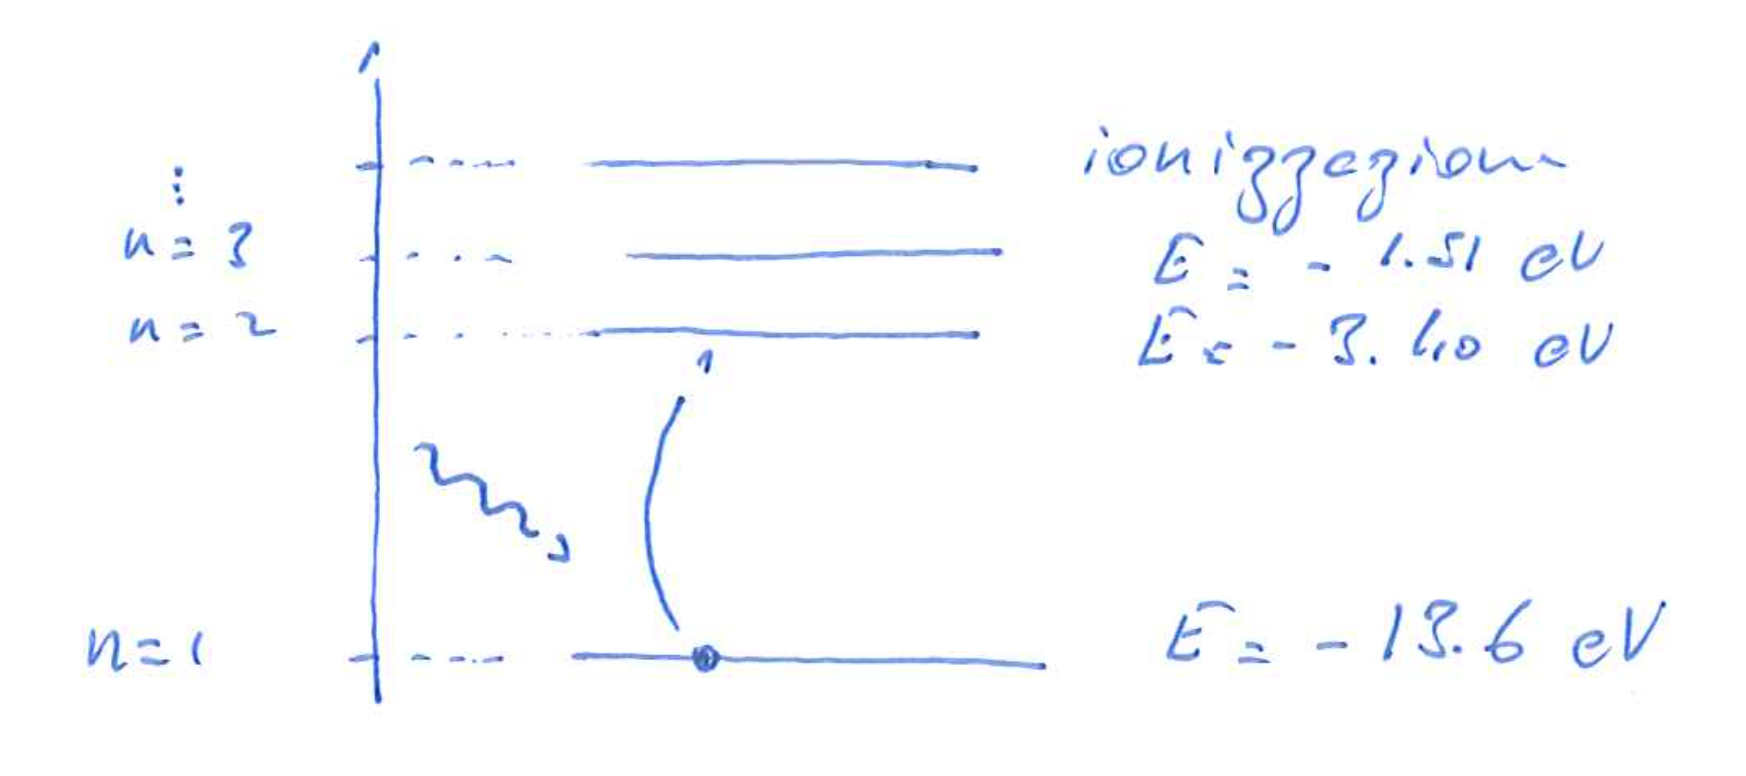
\includegraphics[width=0.8\textwidth]{Hydrogen}
\caption{Structure of the energy levels in an Hydrogen atom}  \label{fig:Hydrogen}
\end{figure}{}

In the case of the Hydrogen atom in its ground state, it should be noted that if energy is given to the system through a photon, with an energy that does not correspond to the difference with its first excited level, the received energy will be transformed only to motion of the hydrogen atom. It is therefore important to cover the widest possible range of energies to ensure that the system does not have an internal structure. \\

The concept of {\it elementary particle} is therefore not definitive and is strictly applicable only for a given range of energies. 
Another way to look at this, which is fundamental in these lectures, is through the quantum nature of microscopic particles and their duality with waves. One starts from the {\it de Broglie} hypothesis that matter particles have a wave-like nature with a wavelength related to their momentum:
$$ \lambda = \frac{h}{p}, $$
which is the generalisation of Einstein's interpretation of the photoelectric effect, whereby electrons can only receive energy in discrete quanta by photons with energy $E = h \nu$, related to the photon frequency $\nu$, and where $h$ is Planck's constant. \\

Heisenberg's uncertainty principle relies on a fundamental hypothesis: it postulates that measuring accurately the position would necessarily disturb the momentum, which could in turn not be measured accurately -- and vice versa:

$$ \Delta p \cdot \Delta x \geq \frac{\hslash}{2}$$

\noindent where $\hslash = h/2\pi$, and $\Delta$ represents the standard deviation of length $x$ and momentum $p$. This view is fundamental in the quantum mechanical interpretation of a particle as a wave. From this principle it is clear that, in order to resolve small distances, large momenta {\it "disturbances"} are needed, and therefore probes (like for example photons) with larger momenta of typically:

$$ p \geq \frac{h}{4\pi x}.$$

Using simple light probes (photons), optical microscopes can naturally resolve structures of the size of approximately \SI{0.2}{\micro\meter}. Electron microscopes (which use as probes electrons) can resolve atomic sizes with resolutions of \SI{0.05}{nm} via Tunnel Transmission Electron Microscopy (TEM). Another sophisticated technique is Scanning Tunneling Microscopy, which makes use of tunnelling electrons, by scanning the material with a conducting tip close to its surface, and applying an electric voltage between the two, thus allowing electrons to tunnel through the vacuum. The position will then be a function of the measured current and the resolution achievable is approximately \SI{0.1}{nm}. See Figure~\ref{fig:Microscope} for an illustration.

\begin{figure}
  \centering
  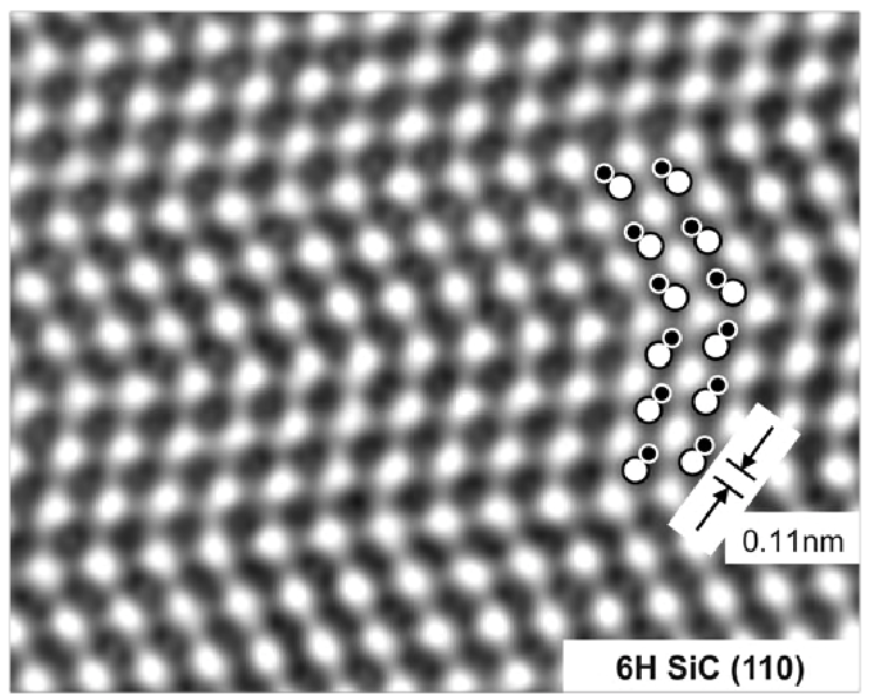
\includegraphics[width=0.4\textwidth]{Microscope-1}
  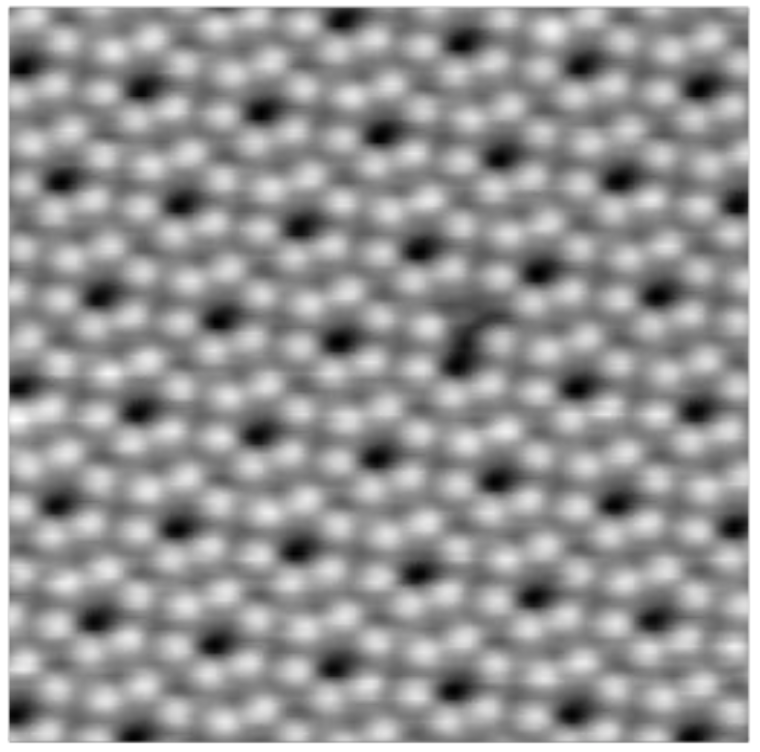
\includegraphics[width=0.4\textwidth]{Microscope-2}
\caption{Example image reconstructed via Scanning Tunneling Microscopy.}  \label{fig:Microscope}
\end{figure}{}

 Higher energies are needed to resolve even smaller distance scales, which requires new sources of particles at higher energies. As we will see in these lectures, a number of such sources have been used.  \\
 
  As will be discussed in Chapter~\ref{decaylaws-I}, the discovery of radioactivity provided sources of photons, electrons and $\alpha$ particles at higher energies (energies which nowadays would be deemed as fairly low!). Another very interesting source of high energy particles, as will be discussed in Chapter~\ref{}, are cosmic rays, which constitute the source of highest energy particles to date. Later, with the development of Nuclear, Subnuclear and Particle Physics came sources of particles at increasingly larger energies, reached through accelerators and eventually colliders. Accelerator techniques will be discussed in Chapter~\ref{accelerators}.

\section{Fundamental Forces}

In his first formulation of a Modern Physics theory of gravitation, Newton recognized immediately that there was a {\it "great absurdity"} in imagining that a force could be acting from one body to another at a distance! As he stated unambiguously in his letter to Bentley in 1692: 

\begin{quote}
    "It is inconceivable that inanimate Matter should, without the Mediation of something else, which is not material, operate upon, and affect other matter without mutual Contact...That Gravity should be innate, inherent and essential to Matter, so that one body may act upon another at a distance through a Vacuum, without the Mediation of any thing else, by and through which their Action and Force may be conveyed from one to another, is to me so great an Absurdity that I believe no Man who has in philosophical Matters a competent Faculty of thinking can ever fall into it. Gravity must be caused by an Agent acting constantly according to certain laws; but whether this Agent be material or immaterial, I have left to the Consideration of my readers."
\end{quote}

Another very important aspect that will be developed in these lectures is that of forces or interactions.

% Always give a unique label
% use \chaptermark{}
% to alter or adjust the chapter heading in the running head

\section*{Take-home lessons}
\begin{itemize}
    \item Modern Physics includes Nuclear and Subnuclear physics; Particle Physics is a branch of the latter, and studies the fundamental components and forces of the Universe.
    \item A particle is considered as elementary if it shows no internal structure, i.e. if one gives energy to that particle, this energy will be used only for the purpose of motion (kinetic energy).
    \item We consider a particle as elementary if no experiment to date has proved it isn't -- so the definition of elementary particle is somehow provisional.
    \item The Heisenberg uncertainty principle implies that, in order to probe smaller distances, we need higher energies.
    \item Radioactivity, accelerators, colliders and cosmic rays are sources of particles of higher and higher energy.
    \item Relativity and Quantum Mechanics are two necessary building blocks of our understanding of elementary particles.
    \item The Standard Model of particle physics is the model which best describes elementary particles and their interactions.
    \item Forces, or interactions, have a range: two bodies A and B cannot interact instantaneously, but they rather exchange particles which mediate that interaction.
\end{itemize}
\section*{Questions}
\begin{itemize}
    \item Let's suppose you have a billiard ball. How can you tell whether it's an elementary particle or not?
\end{itemize}


\begin{thebibliography}{99.}%
\bibitem{Popper:Scientificity} K. Popper, ``The Logic of Scientific Discovery''. Abingdon-on-Thames: Routledge. p. 66. (ISBN 0-41527843-0.)

\bibitem{Feynman:PhysicalLaws} R. Feynman, ``The Character of Physical Law''. Modern Library. ISBN 978-0-679-60127-2.
\end{thebibliography}

%%%%%%%%%%%%%%%%%%%%% chapter.tex %%%%%%%%%%%%%%%%%%%%%%%%%%%%%%%%%
%
% sample chapter
%
% Use this file as a template for your own input.
%
%%%%%%%%%%%%%%%%%%%%%%%% Springer-Verlag %%%%%%%%%%%%%%%%%%%%%%%%%%
%\motto{Use the template \emph{chapter.tex} to style the various elements of your chapter content.}
\chapter{From modern atomism to radioactivity}
\label{Fundamentals-I} % Always give a unique label
% use \chaptermark{}
% to alter or adjust the chapter heading in the running head
\section{Ancient Atomism}

There is a long history of the quest to understand what the fundamental laws of nature are and what things are made of and whether there are fundamental building blocks. In ancient history, these were mostly philosophical questions, but they did spark the curiosity of understanding the how nature fundamentally works, and they did have interesting insights. As a foreword to these lectures we will just very briefly mention the main ideas and philosophers just to give an idea of the times involved. An excellent discussion of the long building of the atomic theory from the ancient atomism to the quantum atom can be found in Ref.~\cite{atomismeantique}\\

The presocratic philosophers in ancient Greece and India were probably the firsts to address these questions nearly three millennia ago.\\
	
%\begin{figure}
%  \centering
%  \includegraphics[width=1.0\textwidth]%{SchoolOfAthens}
%\caption{}  \label{fig:SchoolOfAthens}
%\end{figure}

Thales of Mileto (640-545), the first of the so-called atomists, said ``Water is the first principle of everything''. For Anaximenes (596-595 bc) such unifying unlimited principle must be identified with air.  In his cosmogonic theory, Empedocles (494-434 bc) pretended that
the classic principles are four: earth, water, air, fire.\\

Later on, in ancient Greece, Democritus (470-380 bc) with Leucippus his teacher, the philosophers of the Nature, elaborated the
atomic theory. The question was to know whether matter could be
infinitely divided in smaller parts as believed by presocratics. For the
atomists matter is composed by a very small invisible and
indivisible particle: the atom (meaning indivisible in Greek). Atoms
should be infinite in number, various in shape and moving around in
the void.\\

The atomic view of  matter was however ignored by Plato (428-348
bc) and Aristotles (384-322 bc). Plato tried to describe the
universe in a very imaginative way using five geometrical shapes known
as the Plato's elements. Not long after, Epicurus (341-270 bc) like
Democritus defended the atomic materialist theory believing that
matter is made of indivisible atoms floating in empty space.

\begin{figure}
  \centering
  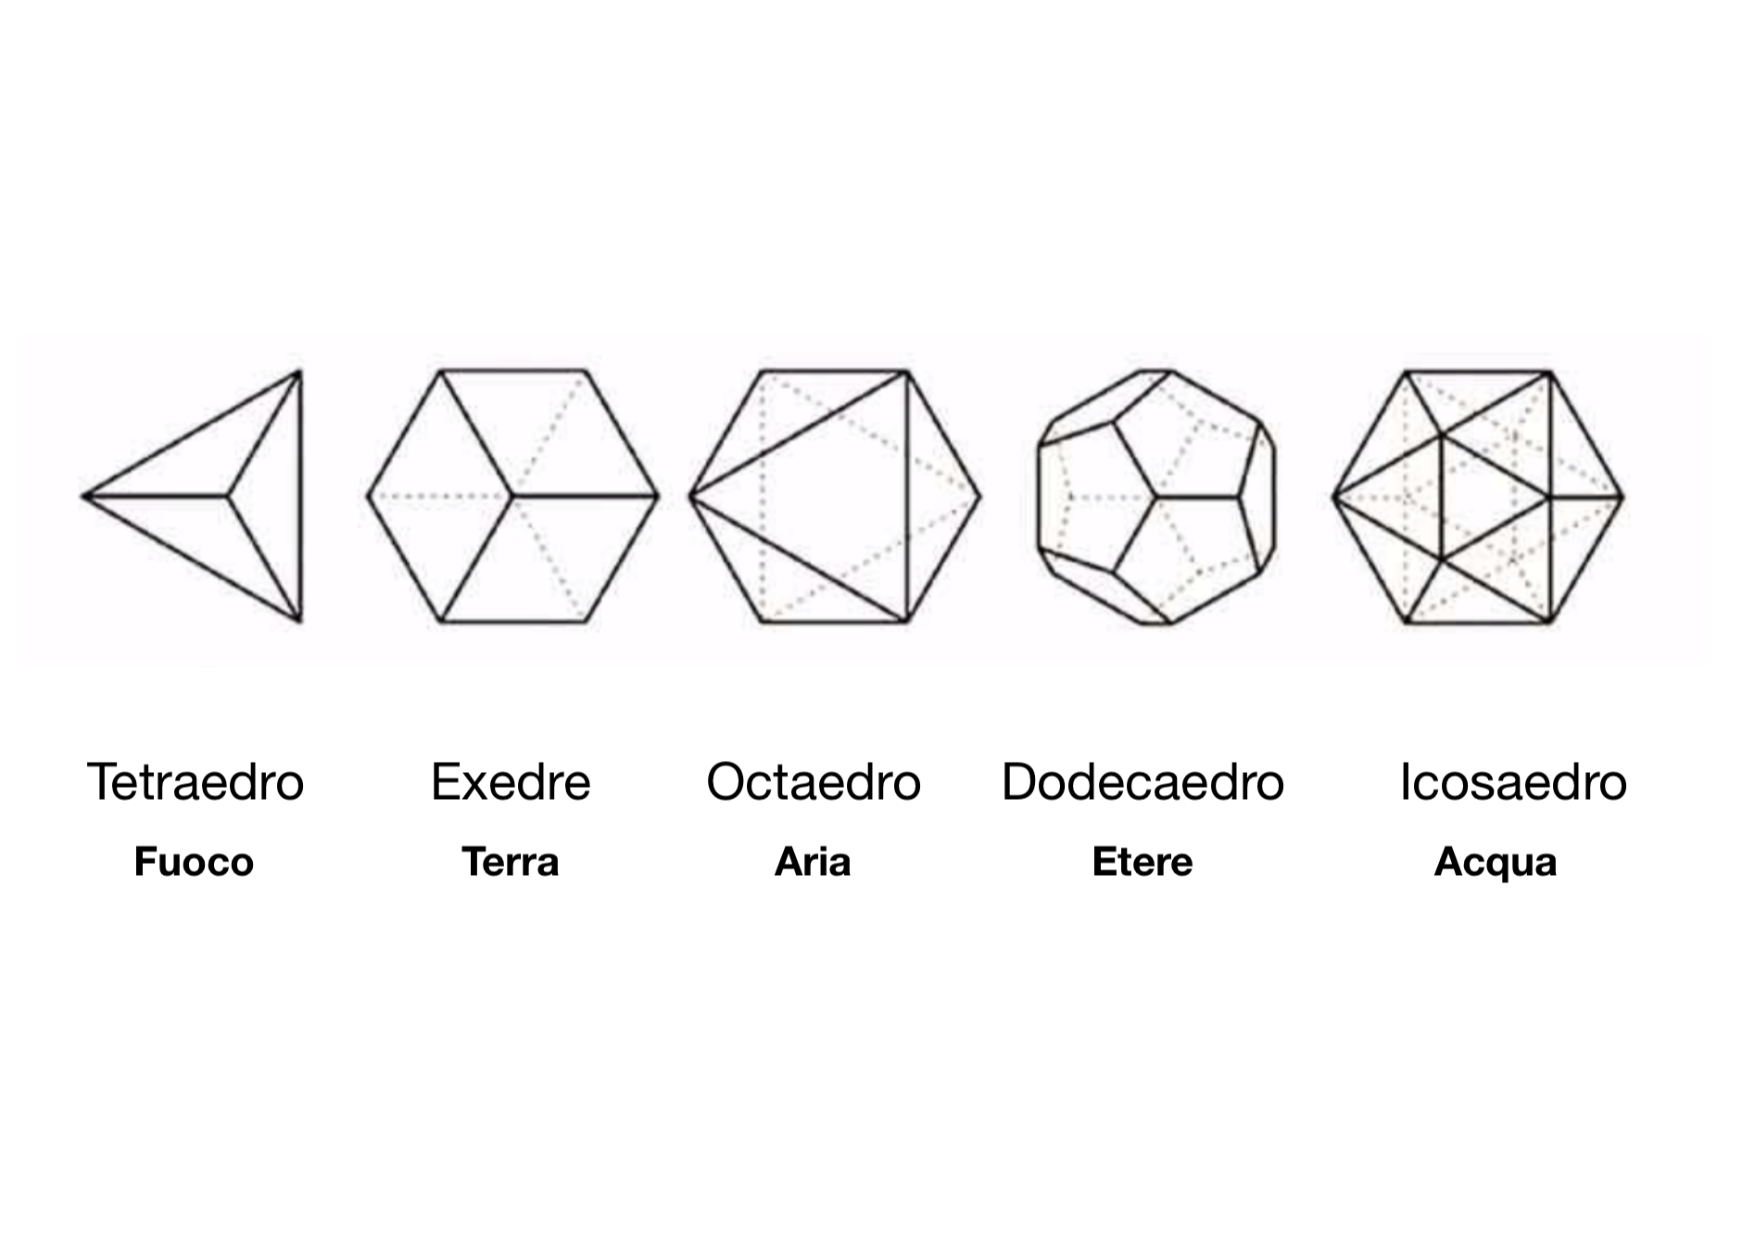
\includegraphics[width=0.8\textwidth]{AncientAtomism}
\caption{The elements from Plato's {\it Timaeus} dialogue, where Plato hypothesized that these regular geometrical forms are the ``classical elements'', i.e. the elements that could explain all complex forms of matter.}  \label{fig:ancientA}
\end{figure}

In Rome, Lucretius (99-55 bc) was the most important nature philosopher and poet, and he was also a definite epicurist. He developed his ideas in six volumes of ``The nature of things'' (\emph{De rerum natur\ae}). He described
the brownian motion of dust particles, taking that as a proof for the existence of atoms. \\

In the ancient Indian philosophy the atomistic theory which appeared
in the VIII century became more elaborated in the I century bc with
the Nyaya naturalists and the Vaisheshikas atomists. \\

The intuitions of the ancient philosophers were remarkable, but at the time they could of course only be philosophical considerations.

\section{Modern Atomism}
\label{Atomism}

The first scientific atomic theory has been proposed in 1803 by John
Dalton. Dalton was an English quacker, a chemist and a meteorologist;
he was color blind and his first paper was on color blindness (which
was called daltonism after him). He also proposed that  matter is made of
blocks of atoms indivisible and indestructible. All atoms of a single
element are identical, whereas atoms of different elements have
different size and mass in order to compose complex structures. 
John Dalton formulated his atomic hypothesis as follows:
\begin{itemize}
    \item matter is made of small particles or atoms;
    \item atoms are indivisible and can neither be created or destructed;
    \item all atoms of an element are identical and have the same mass;
    \item different atoms have different masses;
    \item a compound is made of a fixed number of its constituent atoms (in fixed proportions).
\end{itemize}

It is not completely clear however how John Dalton came to propose his insightful theory. Nevertheless, his theory includes two laws known at the time:

\begin{itemize}

\item The law of mass conservation elaborated and expressed by the
french chemist Lavoisier in 1789, according to which the mass of an
invariant amount of elements remains constant in their chemical
reactions: for example,

		$$ CH_4 + 2O_2 \rightarrow  CO_2 + H_2O.$$

\item The law of definite proportions discovered in 1784 by another French
chemist, Joseph Louis Proust, which states that chemical compounds always combine in constant proportions during chemical reactions  (for example, a fraction of 8/9 -- or to be more explicit 16/18, of the mass of water comes from oxygen and 1/9 from hydrogen).
\end{itemize}

The law of the definite proportions can then be extended to the law of {\it multiple proportions}, stated by John Dalton in 1803, whereby considering two compounds made of two elements A and B (in different proportions), where $r_1, r_2$ are the ratios of the masses of A divided by the masses of B (for each compound $m_A/m_B$), then the ratio $r_1/r_2$ will always be the ratio of small whole numbers. Or in other terms, for any compounds of elements A and B composed by \SI{1}{g} of A, where A is the lightest element between A and B, will require an integer number of grams of B.\\

As an example, let's consider nitrogen (N) and oxygen (O) in the reactions:

$$ 4NO + 2O_2 \rightarrow 4N_2O_3 \; \; {\rm (proportion \; of \; 2:1 \; between} \; 
NO \; {\rm and} {\rm \;O_2)} $$
   
$$ 4NO_2 + 2O_2 \rightarrow 4NO_2  \; \; {\rm (proportion \; of \; 2:1 \; between} \; NO_2 \; {\rm and} \; {\rm O_2 \;)} $$ 

As it is apparent in this example, the possibility that elements could make compounds by themselves such as $O_2$ was not yet taken into
consideration. From the above laws, John Dalton assigned an integer number to elements, by comparison between elements that form compounds. This integer number was referred to as \emph{atomic mass}. In his classification of elements, hydrogen was the lightest and was assigned an atomic mass of 1. Given that hydrogen combines with oxygen in a ratio of masses of 1 to 7, Dalton assigned an {\it atomic mass} of 7 to oxygen, and so on an so forth (see Table~\ref{tab:DaltonElements}). \\

\begin{table}[h]
    \centering
    \begin{tabular}{l c | l c}
    \hline \hline
    Elements & A.M. & Elements & A. M. \\ \hline
    Hydrogen & 1    & Strontian & 46 \\
    Azote  & 5      & Barytes   & 68 \\
    Carbon  & 5     & Iron      & 50 \\
    Oxygen & 7      & Sinc      & 56 \\
    Phosphorous & 9 & Copper    & 56 \\
    Sulphur & 13    & Lead      & 90 \\
    Magnesia & 20   & Silver    & 190 \\
    Lime & 24       & Gold      & 190 \\
    Soda & 28       & Platina   & 190 \\
    Potash & 44     & Mercury   & 167 \\
                 \hline \hline
    \end{tabular}
    \caption{Table of atomic masses (A. M.) of elements according to John Dalton. Azote is the Greek name of nitrogen $\alpha\zeta\omega\tau\iota\kappa o \sigma$ used then by Dalton, and still in use in Italian, French and various other languages.}
    \label{tab:DaltonElements}
\end{table}

This was then resolved in steps. The first was the ideal gas law of Gay-Lussac,:

$$PV = nRT,$$

\noindent where $P$ is the pressure of a gas, $V$ is its volume, $T$ its temperature and $R$ the universal gas constant ($R=8.314$~J/K/mol), and $n$ is the {\it amount of substance} measured in number of moles. Moles are just a unit of number of entities of a substance, defined by the Number of Avogadro (${\mathcal N}_A = 6.02 \times 10^{23}$). This law is known to be correct only in the limit of small densities. This very useful formula in chemistry has actually very far-reaching consequences in the construction of a modern atomic theory. What it is really stating is that in the limit of small densities and at equal pressures, volumes and temperatures, the number of molecules in different gases are equal! \\

This was recognized by Avogadro in 1811 when he proposed that two identical volume of different gas contain the same number of
``particles''. Therefore, in modern terms, the mass has no impact on the volume. Identical volumes of different gas contain the same number of molecules at a given pressure and temperature. As illustrated in figure~\ref{fig:Volumes}, two volumes of $H_2$ are needed for one volume of $O_2$ to make two volumes of $H_2O$. This reaction implies that the oxygen in the initial state has to be forming molecules of two oxygen elements $O_2$. \\
	
\begin{figure}
  \centering
  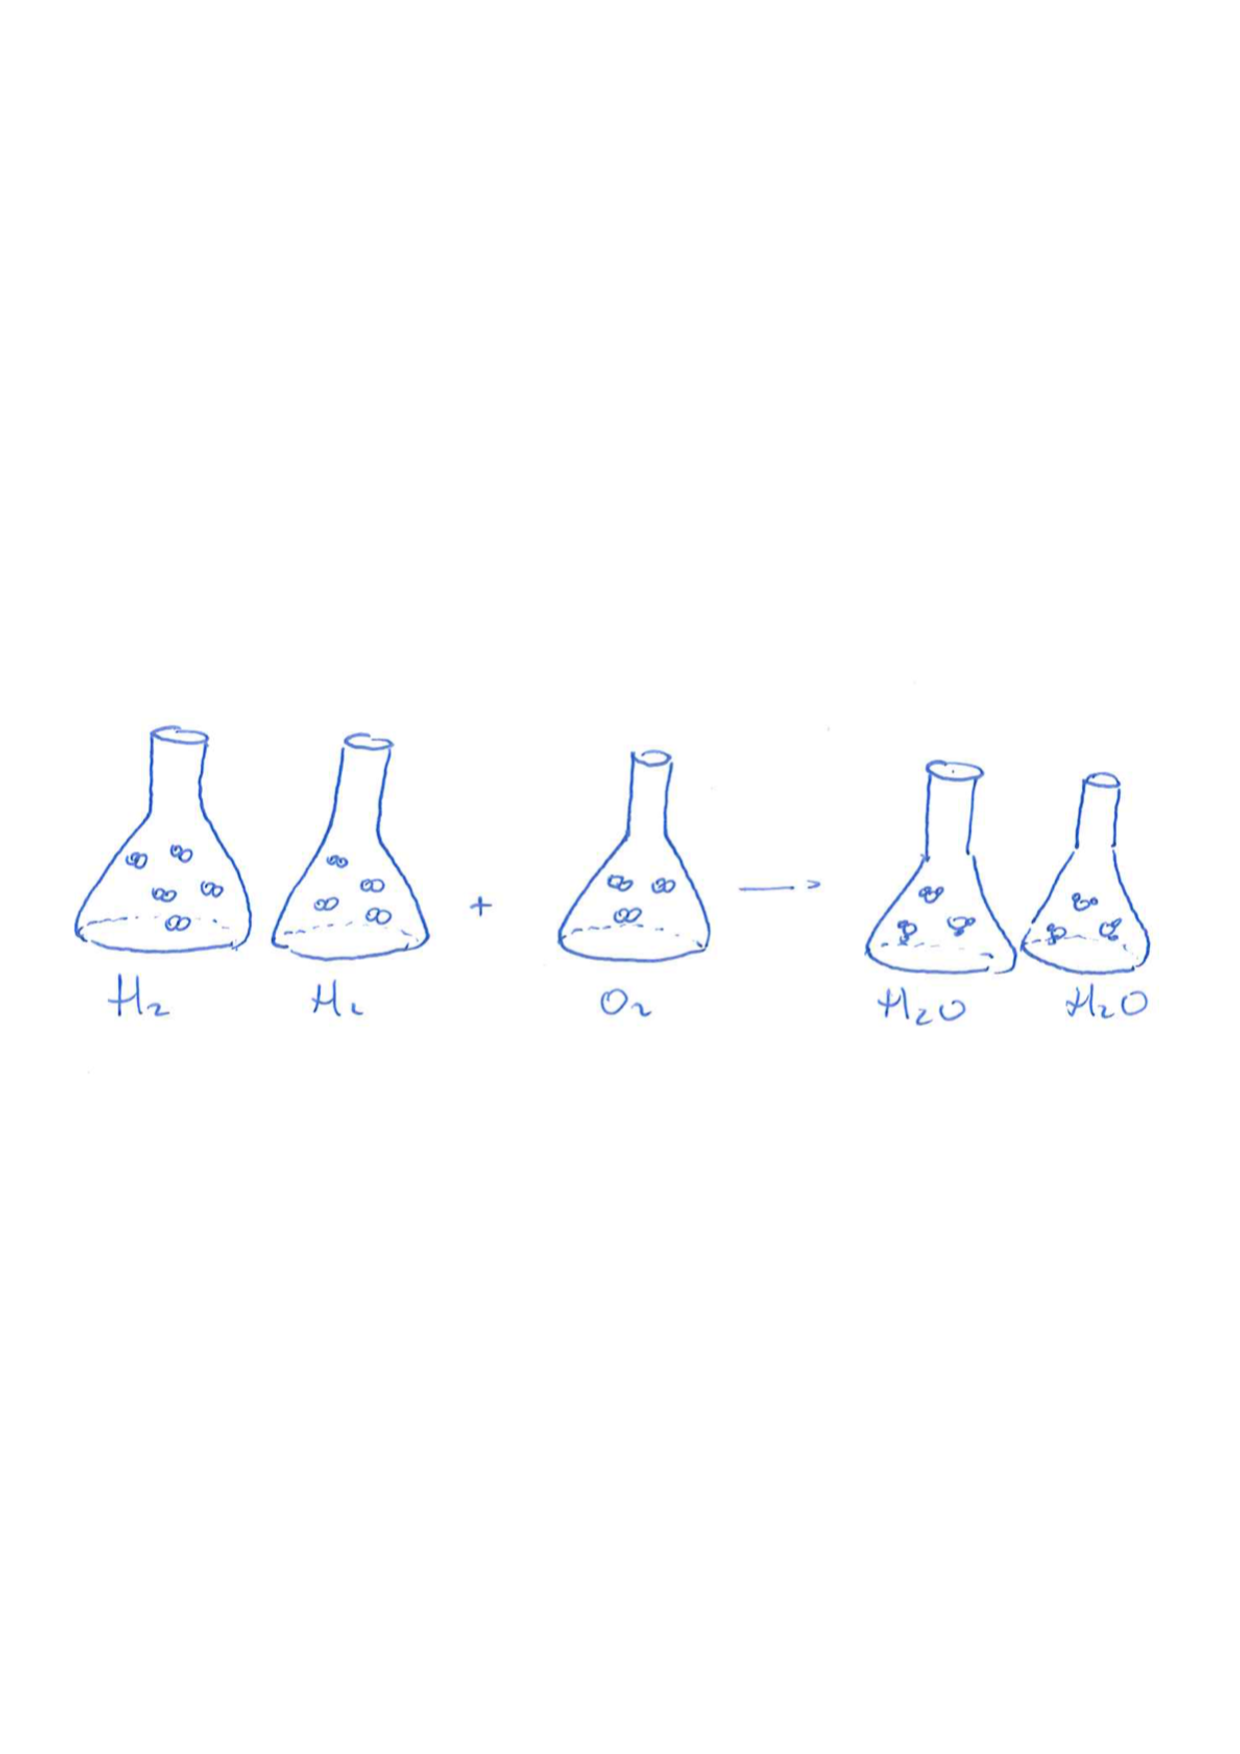
\includegraphics[width=0.8\textwidth]{Volumes}
\caption{Illustration of the implication of the ideal gas law and interpretation by Avogadro that identical volumes of different gases, at given temperature and pressure, contain the same number of entities or ``particles''.}  \label{fig:Volumes}
\end{figure}{}

\section{The proton}
From the laws and the classification in Section~\ref{Atomism}, all elements have  integer atomic masses -- or, in other terms, all elements have masses multiple of the ``first'' element, i.e. hydrogen. In Greek, ``first'' translates to \emph{protos} ($\pi \rho \tau\omicron \sigma$), or \emph{proton}, as the first in the composition of elements. This is a formidable insight in what will then be understood as the structure of the atomic nucleus. \\

\subsection{Atomic mass}
It is interesting to note that while the first element is hydrogen, and was chosen to be the unit of atomic mass by John Dalton, in 1865 the atomic mass unit was chosen to be 1/16$^{\rm th}$ of the oxygen mass, due to the fact that oxygen was very prominently present in a large number of reactions. Current units of {\it atomic mass} are (since 1971) based on Carbon (on its $^{12}C$ isotope, to be precise) due to its very high abundance, high stability and the fact that it has the same number of protons and neutrons (these notions will be more detailed in these lectures). \\

In order to count the number of entities or particles of a substance, at the time the concept of {\it mole} was introduced. It is intrinsically related to the concept of atoms or particles: the idea is to know how many entities are included in one unit of a given element, where that unit is taken to be \SI{12}{g} of $^{12}C$. That is almost equivalent to \SI{1}{g} of hydrogen. \\

To avoid confusion, let's have a brief reminder of some of the related fundamental concepts. If we call $m$ the mass of a sample of a given substance, $m$ is related to the number of entities or particles of the substance, $n$, via its {\it molar mass} $M$, through the relation

$$m = M \cdot n.$$ 

The molar mass, expressed in \si{g/mol}, is the mass of a mole of a given substance. \\

The atomic mass unit, was defined until 2019 to be precisely 1/12 of the mass of a carbon atom. Therefore, until then the mass of \SI{1}{mol} of carbon was precisely equal to \SI{1}{g}. Since 2019, the {\it unified} atomic mass unit was set to be a constant, instead of being fixed to the mass of a given substance:

$$m_u = \SI{1.660539066605e-27}{kg}.$$ % 1.660 \, 539 \, 066 \, 60 \, (5) \times 10^{-27} \; {\rm kg}$$ 

Its numeric value is essentially extremely close to $1/12$ of the mass of a Carbon atom, but it is set as a constant.\\

A simple way to estimate the Avogadro number is taking a given volume of oil (knowing the mass and the nature of the substance) and let it cover a given surface on water. Assuming that the layer is mono-molecular, one can derive the Avogadro number from the measurement of the surface covered by the thin layer of oil. There are of course many more subtle ways to determine the Avogadro number that are beyond the scope of these lectures, the most precise coming from the study of Brownian motion. The current value is:
\begin{equation}
    {\mathcal N}_A = \SI{6.022140857(74)e23}{mol^{-1}}.% 6.022 \, 140 \, 857 \,(74) \times 10^{23} {\rm [mol^{-1}]}
\end{equation}

In this case as well, since 2019 the Avogadro number was fixed to be a constant, precisely:

\begin{equation}
    {\mathcal N}_A = \SI{6.02214076e23}{mol^{-1}}.
\end{equation}

\subsection{The Faraday experiment and the ``charge'' of atoms}

In his insightful electrolysis experiments, in 1830 Michael Faraday published two very important laws on electrolysis that can be summarised in one. \\

\begin{quote}
{\bf Faraday's first law of electrolysis}: the amount of mass deposited on an electrode, due to the flow of current through an electrolyte, is directly proportional to the quantity of electricity that passed through it.
\end{quote}

\noindent The second is a bit more quantitative and also extremely important.

\begin{quote}
{\bf Faraday's second law of electrolysis}: 
when the same quantity of electricity is passed through several electrolytes, the mass of the substances deposited are proportional to their respective equivalent mass.
\end{quote}

\noindent Here the {\it equivalent weight} is the ratio between the mass of the atom and its valence, and the valence is defined as the number of hydrogen atoms with which it can combine. \\

These laws can be illustrated with a simple example: a battery with a Copper Sulfate solution ($CuSO_4$) and two copper electrodes. The observation is that a mass of copper has moved from the anode (+) to the cathode (-). The idea is that, with the electric tension applied between the two copper plates, $Cu^{2+}$ ions are dissolved in water and move towards the cathode. The valence in this case is very important to assess the amount of mass deposited with respect to charge. The valence of copper is $2$. \\

According to these laws, one mole of an element attracted to one of the electrodes will correspond to a definite amount of charges, and in the case of a mono-valent element one has
\begin{equation*} F = 96 485 \; {\rm C/mol},\end{equation*}
i.e. the Faraday constant, which gives the charge corresponding to one mole of element deposited on the electrode. This formula can be generalized to
\begin{equation*}
m = \frac{M q}{F Z},
\end{equation*}
where $Z$ is the electrolyte valence, $M$ the molar mass, $q$ the total charge and $m$ the deposited mass, and $F$ the Faraday constant.

This is very far reaching, since it provides a definition of the unit charge corresponding to a monovalent element, which can be given by:
\begin{equation*}
e = \frac{F}{\mathcal{N}_A} = \SI{1.60e-19}{C},% \times 10^{-19} C
\end{equation*}
which can easily be derived from the simplest system -- the hydrogen atom -- which is monovalent and has a molar mass of approximately $1$. \\

The idea that all atoms could be made of hydrogen was proposed in 1815 by William Proust. The idea emerged that there was a form of unit charge $e$: the concept of \emph{proton}, with unit mass and unit charge, was starting to take shape. However. the discovery of the proton was published in 1919 from the experiment made by Ernest Rutherford two years earlier. This discovery came after the discovery of the existence of the nucleus in 1911, also by Ernest Rutherford.

\begin{framed}
    \begin{experiment}[Discovery of the Proton - Ernest Rutherford, 1919]

Bombarding nitrogen atoms with alpha particles, Ernest Rutherford obtained the following reaction:
		\begin{equation*}\alpha + ^{14}N  \rightarrow  O + p,\end{equation*}
where protons were found to be able to cover long distances.
\end{experiment}

\end{framed}
In the meantime, many other key discoveries which will be discussed in this chapter were made.

\section{Atomic Classification}
A large fraction of the work of the XIX century in Chemistry was devoted to study the physical properties and the reactions of as many substances as possible. A large number of new elements and compounds were discovered. \\

With the massive amount of data and the simple laws stated above, a classification of their properties could be made, according to their atomic masses and their valence. \\

It was the Russian Physicist Dmitri Mendeleev who first started a systematic classification of elements according to their masses and their chemical properties. After a first attempt in 1869, in 1871 he published a classification that highlights the importance of  atomic valence. In his work, valence is reflected in the number of elements with which an element can combine, and can be used to classify the elements according to their electronic valence based on how elements combine with hydrogen and ($H$) and oxygen ($O$). For example, $H$ is mono-valent as it combines with another $H$ to for $H_2$, and therefore $O$ has a valence of II since it combines with two $H$ to form $H_2O$. Elements $El$ that combine with one H to form $ElH$ or with one $O$ to form $El_2O$ have a valence of I. Elements forming $ElO$ or $H_2El$ have a valence of II. Elements forming $El_2O_3$ or $ElH_3$ have a valence of III, and so on and so forth. A classification is shown in Table~\ref{tab:mendeleev}.

\begin{center}
\begin{table}
\begin{tabular}{c cl}
 Valence && Elements \\\hline
 0 && He, Ne, Ar, Kr, Xe, Rn \\
 I &&  H, Li, Na, K, Rb, Cs, Fr, Cu, Ag, Au, F, Cl, Br, I \\
 II && Be, Mg, Ca, Sr, Ba, Ra, Zn, Cd, Pt, Hg, Sn, Pb, O, Se, Te, C \\
 III && B, Al, Au, Fe, Co, Ni, Cr, Mn, Cl, Br, I, Ga, In, Tl, N, P, As, \\ 
 && Sb, Bi, Po \\
 IV && C, Si, Ge, Sn, Pb, S, Se, Te, Pt, Ir, Mn \\
 V && Bi, Sb, As, I, Br, Cl, P \\
 VI && Te, Se, S, Mn, Cr \\
 VII && Mn, Cl, Br, I \\
\end{tabular}
\caption{Classification of elements by Mendeleev, according to their valence.}\label{tab:mendeleev}
\end{table}
\end{center}

Mendeleev soon noticed that elements could be classified according to the number of hydrogen and oxygen elements with which they can combine. In this classification he had eight columns which showed an intriguing {\bf periodicity}, as shown in Table~\ref{tab:FirstPeriodicTable}.

\begin{table}[]
    \centering
    \begin{tabular}{c|c|c|c|c|c|c|c|c}
     \hline  \hline
        \hspace{0.5 cm} & I & II & III & IV & V & VI & VII & VIII \\
         & $El_2O$ & $El O$ & $El_2 O_3$ & $El H_4$ & $El H_3$ & $El H_2$ & $El H$ & $El O_4$ \\  \hline
         \multirow{2}{*}{1} & H & \multicolumn{6}{c}{}  \\
           & 1 & \multicolumn{6}{c}{} \\     \cline{1-8}
         \multirow{2}{*}{2} & Li & Be & B & C & N & O & F & \\
           & 7 & 9.4 & 11 & 12 & 14 & 16 & 19 & \\  \cline{1-8}
         \multirow{2}{*}{3} & Na & Mg & Al & Si & P & S & Cl & \\
           & 23 & 34 & 27.3 & 38 & 31 & 32 & 35.5 & \\     \hline
         \multirow{2}{*}{4} & K & Ca &  & Ti & V & Cr & Mn & Fe, Co, Ni \\
           & 39 & 40 & & 48 & 51 & 52 & 55 & 56, 59, 59 \\     \hline
         \multirow{2}{*}{5} & Cu & Zn & (Ga) &  & As & Se & Br & \\
           & 63 & 65 & 68 & 72 & 78 & 78 & 80 & \\     \hline
         \multirow{2}{*}{6} & Rb & Sr & Yt & Zr & Nb & Mo & & Ru, Rh, Pd \\
           & 85 & 87 & 88 & 90 & 94 & 96 & 100 & 104, 104, 106 \\    \hline 
         \multirow{2}{*}{7} & Ag & Cd & In & Sn & Sb & Te & I & \\
           & 108 & 112 & 113 & 118 & 122 & 125 & 125 & \\     \hline \hline
    \end{tabular}
    \caption{Early Mendeleeev classification of atomic elements (denoted ($El$) according to how they form compounds with hydrogen and oxygen.}
    \label{tab:FirstPeriodicTable}
\end{table}

This first classification starts with a column of alkali metals ($Li$, $Na$, $K$) which have the same valence as hydrogen (these metals have low density and low fusion point). Those appearing in the column VII are the halogens ($F$, $Cl$, $Mn$, $Br$), they easily form compounds with alkalis to form salts (e.g. $NaCl$) and can form bi-atomic gases (e.g. $Cl_2$). Then all elements are ordered according to their atomic masses. This first purely phenomenological classification showed a relation between the atomic mass and chemical properties, and already allowed Dmitri Mendeleev to predict elements in the missing spots in the table. One of them was gallium, which was discovered soon after in 1875 by Lecoq de Boisbadran, and happened to have all the properties predicted by Mendeleeev! This classification also led to introduce the {\bf Atomic Number} which corresponds to the rank of the elements in this periodic table.

Mendeleev's work eventually led to the current grouping in the periodic table of elements, shown in Table \ref{fig:PeriodicChart}. Elements are ordered in terms of their atomic number which is growing by one unit from left to right and top to bottom. The table is further organized in groups of elements with the same valence in columns. It can also be divided in blocks which correspond to the subshell according to the angular momentum $\ell$: the $s (\ell =0)$ subshell corresponds to the two first columns -- including $He$ which has two electrons and completes $1s
^2$, then the elements with their last electrons are in the $p (\ell =1)$ subshell which correspond to the last six columns in the first five rows (excluding $He$), and the elements with their outermost electrons in the $d (\ell =2)$ subshell which corresponds to the 10 middle columns, then the $f (\ell =3)$ is inserted between the $s$ and the $d$ blocs, etc. This classification has been crucial in order to build a quantum theory of the atom. 

\begin{figure}
  \centering
  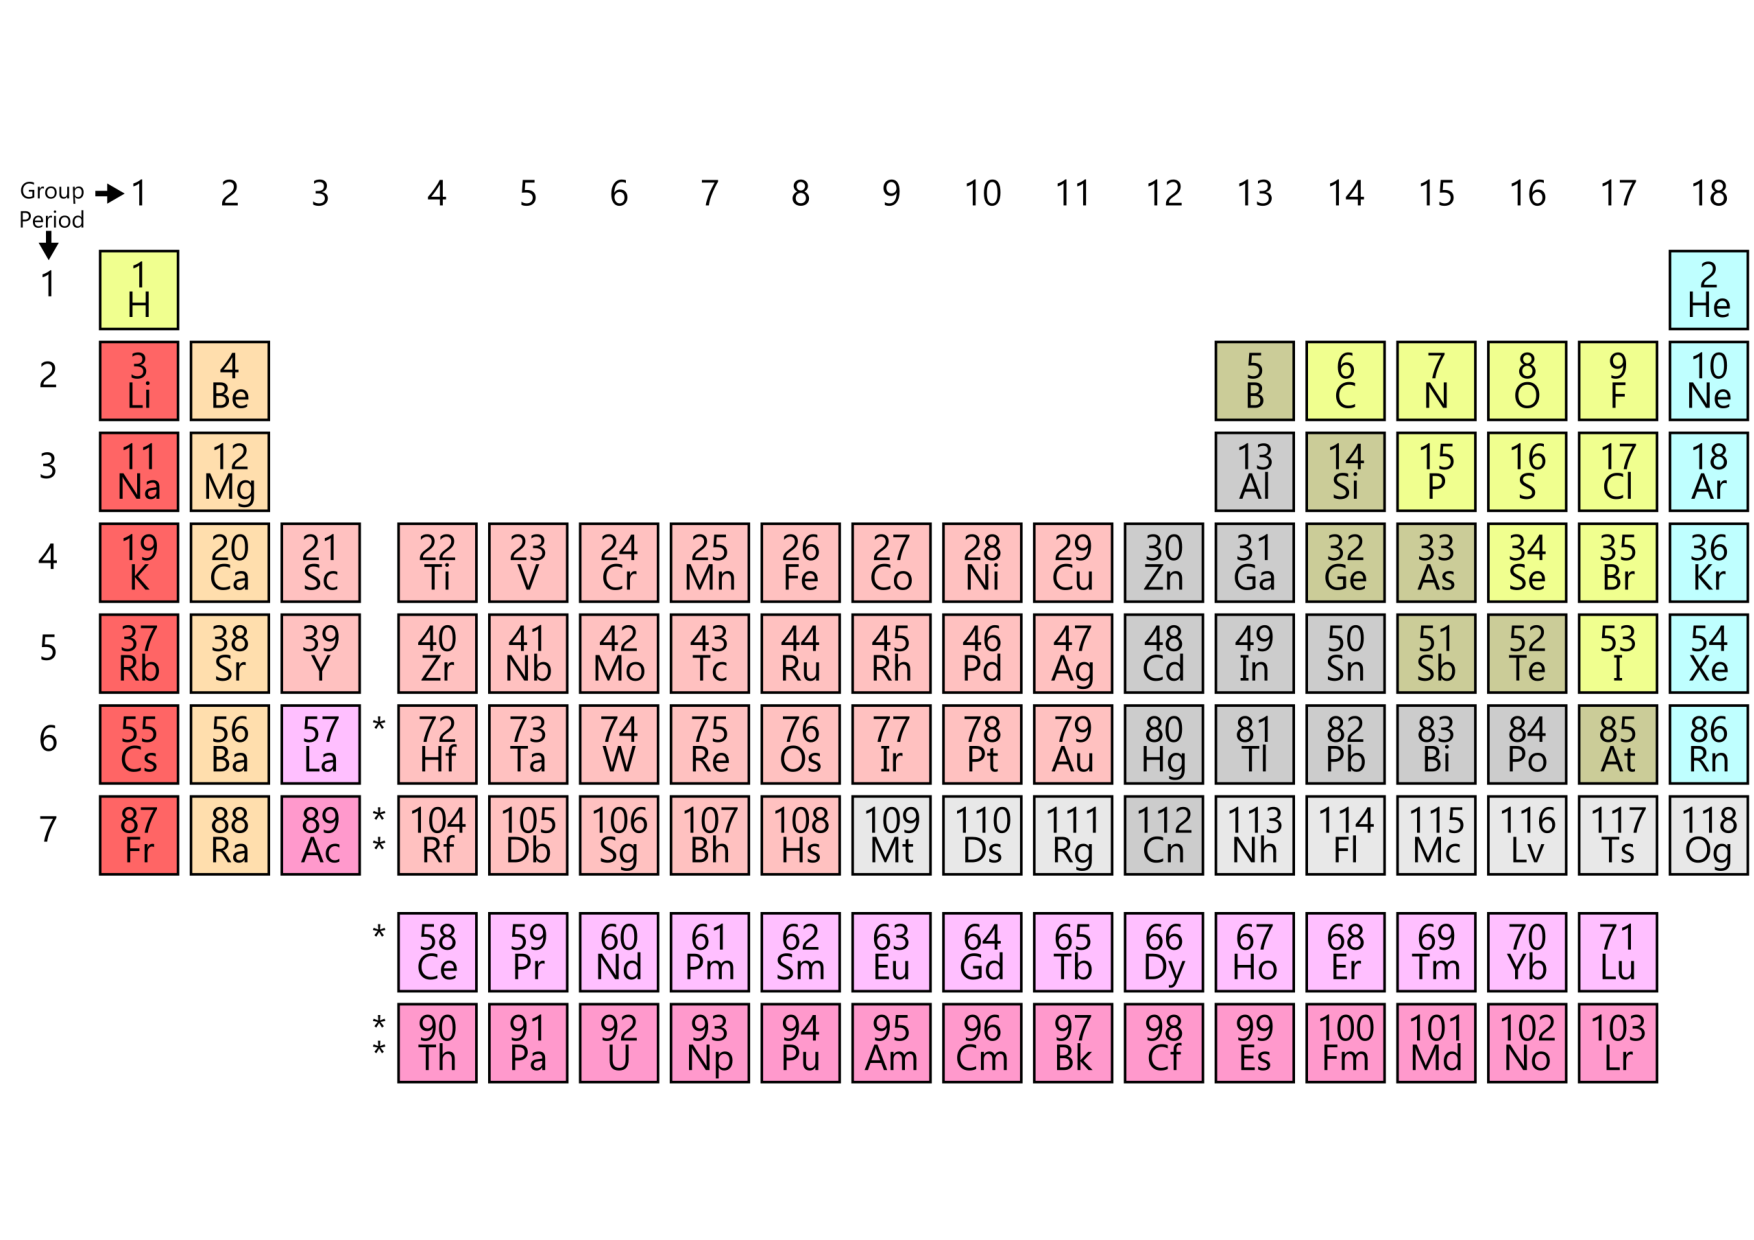
\includegraphics[width=1.0\textwidth]{PeriodicChart}
\caption{Periodic chart of the chemical elements ordered according to their atomic number and electron configuration properties.}  \label{fig:PeriodicChart}
\end{figure}


\section{The Modern Atomic Theory}
In 1827 Robert Brown, a botanist, observed through a microscope that particles of pollen grains of the size of approximately tens of microns in suspension in a fluid, were moving randomly. It was a striking observation that he could not interpret. \\

It was not until 1905 when, in one of his {\it annus mirabilis} papers, Albert Einstein~\cite{BrownianMotion} was able to demonstrate that this motion can be due to the motion of molecules (as for example water molecules in which the pollen particles are suspended), thus demonstrating the existence of atoms. In 1908 Jean Perrin performed a series of measurements that corroborated Einstein's theory stating that it ``cannot leave any doubt of the rigorous exactitude of the formula proposed by Einstein''.

\section{The Discovery of radioactivity}
During the XIX century many discoveries rest on the modern atomic physics and depend on the development of the vacuum tube technologies, namely on the cathode-ray tube. Starting in 1857, Gaissler introduced the glass tube, with two electrodes on each end, to study the electroluminescent discharges. With the help of a vacuum pump he could study the discharge as a function of the gas pressure. Applying high voltage with very low gas pressure, a green luminescence was still obtained on the side of the positive anode. The effect was independent of the presence of residual gas in the tube and of the substances with which the electrodes were made. In 1878 Crookes introduced a fluorescent screen near the anode and demonstrated that the luminescence was associated to the propagation of a kind of ray that could be absorbed by an obstacle generating a shadow on the screen. He could furthermore establish that those cathode rays were deviated by a magnetic field.

\subsection{The discovery of X-rays}
Thomson had not yet described the nature of the cathode rays, when Wilhelm R\"ontgen, a German physicist, on November 8, 1895 discovered that they were producing another type of penetrating radiations invisible to the naked eye depending on the stratification of the material exposed: he gave them the name of X rays. Unlike cathode rays, they could pass through the matter coloring selectively a fluorescent screen or a photographic plate. X rays immediately became widely known because of their ability to visualize bones inside the human body, and R\"ontgen had found this phenomenon experimenting on himself almost by chance. Today we know that cathode rays are electrons, and that X rays are photons irradiated by impinging electrons because of the strong deflection in the atomic nuclei of the anode, which induces bremsstrahlung emission of photons (continuous spectrum), or when the impinging electrons remove electrons from the internal layers, with the release of photons as transition from the external electrons toward the relative gap with energy corresponding to the difference between the two electron levels (striped spectrum). \\
\begin{framed}

\begin{experiment}[Discovery of X-rays - Willhelm R\"ontgen, 1895]

\begin{center}
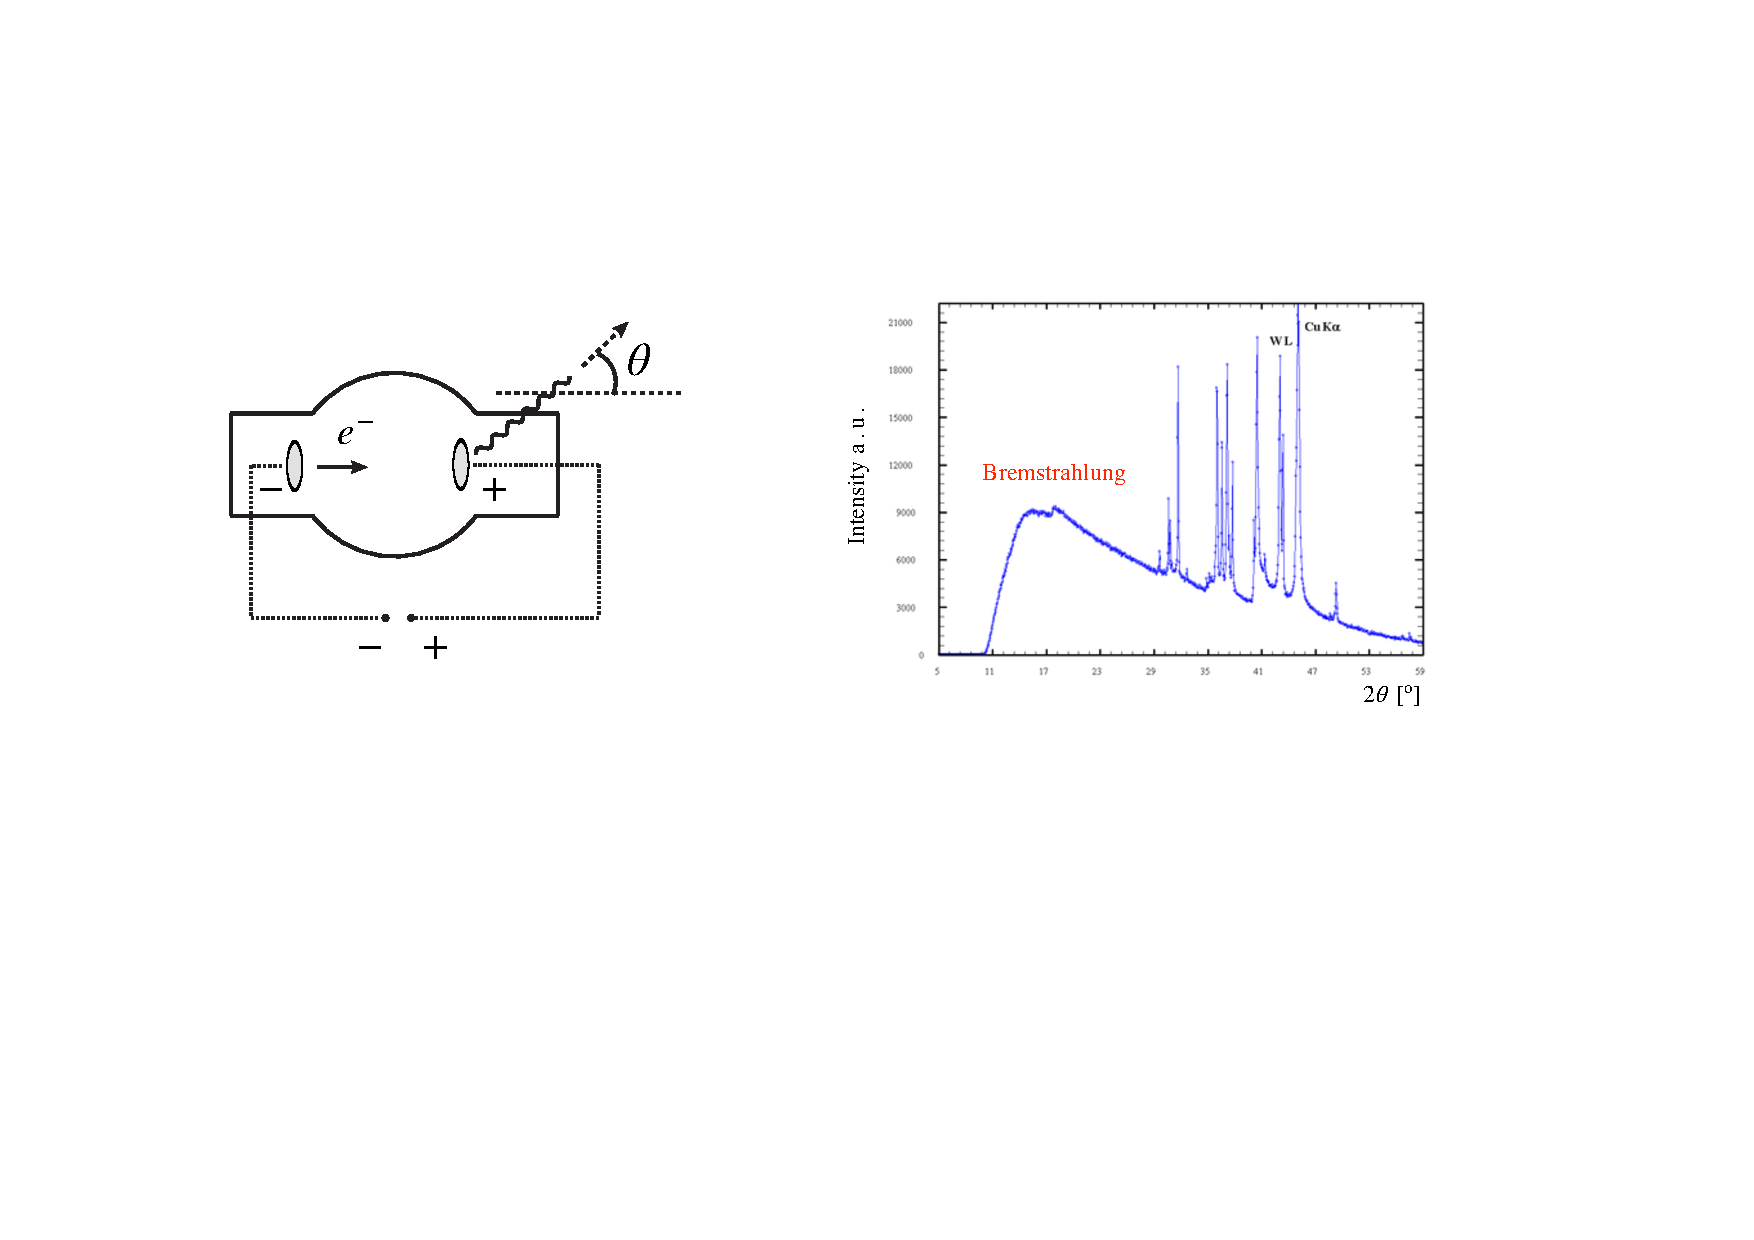
\includegraphics[width=0.95\textwidth]{X-ray-1}
\end{center}

Top: A cathodic tube used by Crooks: the metal Maltese cross was used to demonstrate the cathode ray absorption by the metal of the cross, as it gave a shadow on the fluorescent screen (on the left). This was used as a proof of the fact that cathode rays propagate on a straight line.

Bottom: two examples of X ray production. On the left, the impinging electron kicks off an electron of an inner layer, and a photon is emitted when another electron from the next layer fills the gap. On the right, the photon is instead emitted by the bremsstrahlung of the impinging electron, whose path is deflected by the atomic nucleus.
\begin{center}
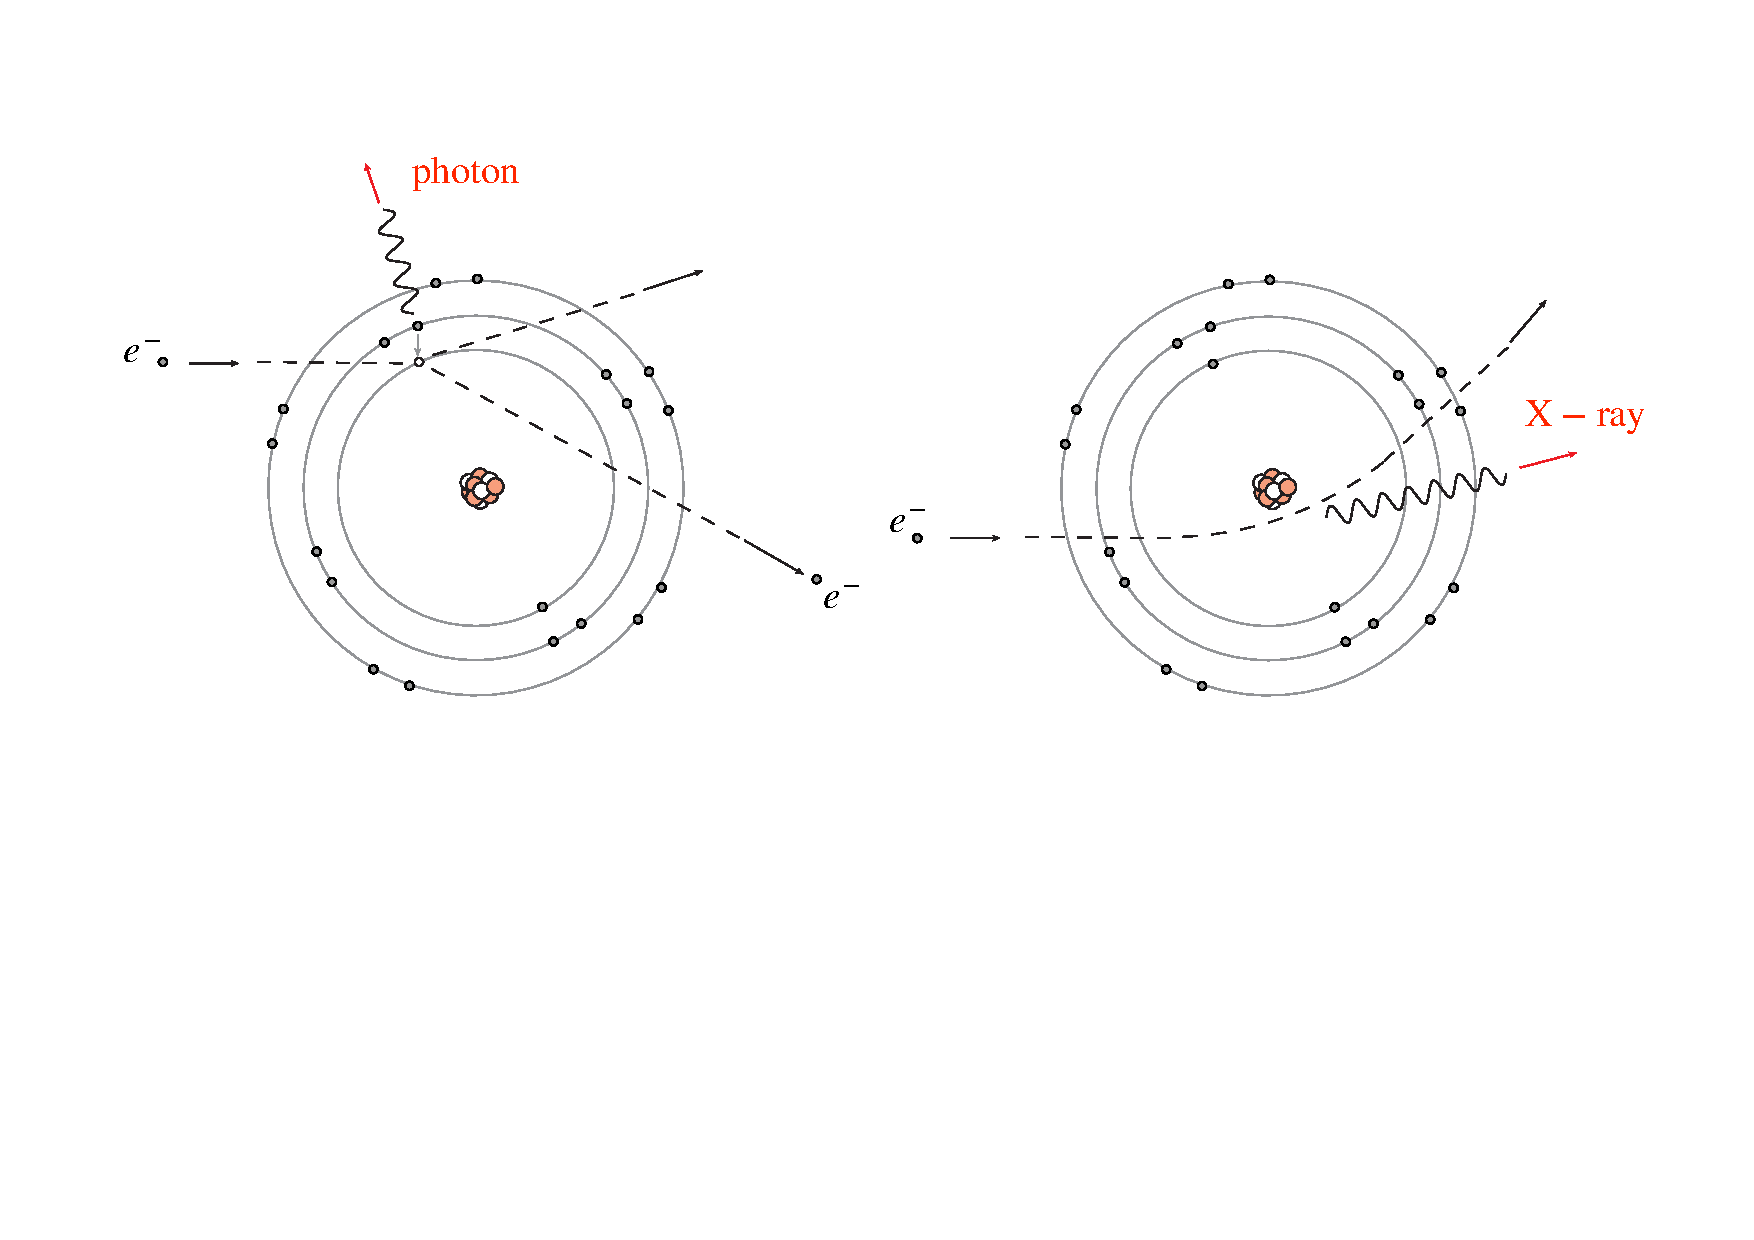
\includegraphics[width=.9\textwidth]{X-ray-2}
\end{center}

\end{experiment}
\end{framed}


\subsection{The discovery of radioactivity and $\alpha$-, $\beta$- and $\gamma$-rays}
\label{sec:DiscoveryRadioactivity}

The intense developments and research in Physics and Chemistry towards the end of the XIX century, led to a ground breaking and completely unexpected discovery. \\

The French physicist Henri Becquerel, who was interested in phosphorescence phenomena, was seeking for a connection between the phosphorescence of uranium salts and possible emission of the recently discovered X-rays. As in the case of phosphorescence, Becquerel was expecting the phenomena to appear after the exposure of the uranium salts to sunlight. \\

\begin{framed}

\begin{experiment}[Discovery of Radioactivity - Henri Becquerel, 1896]


In 1896, Henri Becquerel exposed various salts among which Potassium Uranium Sulfates to sunlight before placing them in front of photographic plates protected from light by black paper. All results failed, except those related to the Potassium Uranium Sulfates. While things were proceeding according to plan, on February 26 -- a cloudy day in Paris (like it's usual in that period of the year) --  Becquerel placed his salts and photographic plates in a closet. On March 1, by scientific rigor, Becquerel decided to develop the photographic plates. Much to his surprise, the images were clearly impressed and even even the shape of a copper cross which had been placed by chance between the salts and the plate was impressed. Becquerel had discovered natural and spontaneous radioactivity (the term \emph{radioactivity} was given by Maria Sklodowska-Curie). The conclusion was that the material was spontaneously emitting radiation which had properties similar to X rays.
\end{experiment}
\end{framed}

In 1898 Maria Sklodowska-Curie, in collaboration with her husband Pierre Curie, working on an uranium mineral extracted from uranite (or pitchblende), demonstrated that a radioactivity much more intense than the one due to the uranium salts was associated to two chemical elements not known until then, which they called polonium and radium. \\

The same year Ernest Rutherford demonstrated that natural radioactivity observed at that time was due to radiation different from X rays. To further study the nature of these spontaneously-emitted radioactive rays, Rutherford built a device which used led to collimate the rays and study their behaviour under magnetic field (see Fig.~\ref{fig:Radioactivity}).  \\

\begin{figure}
    \centering
      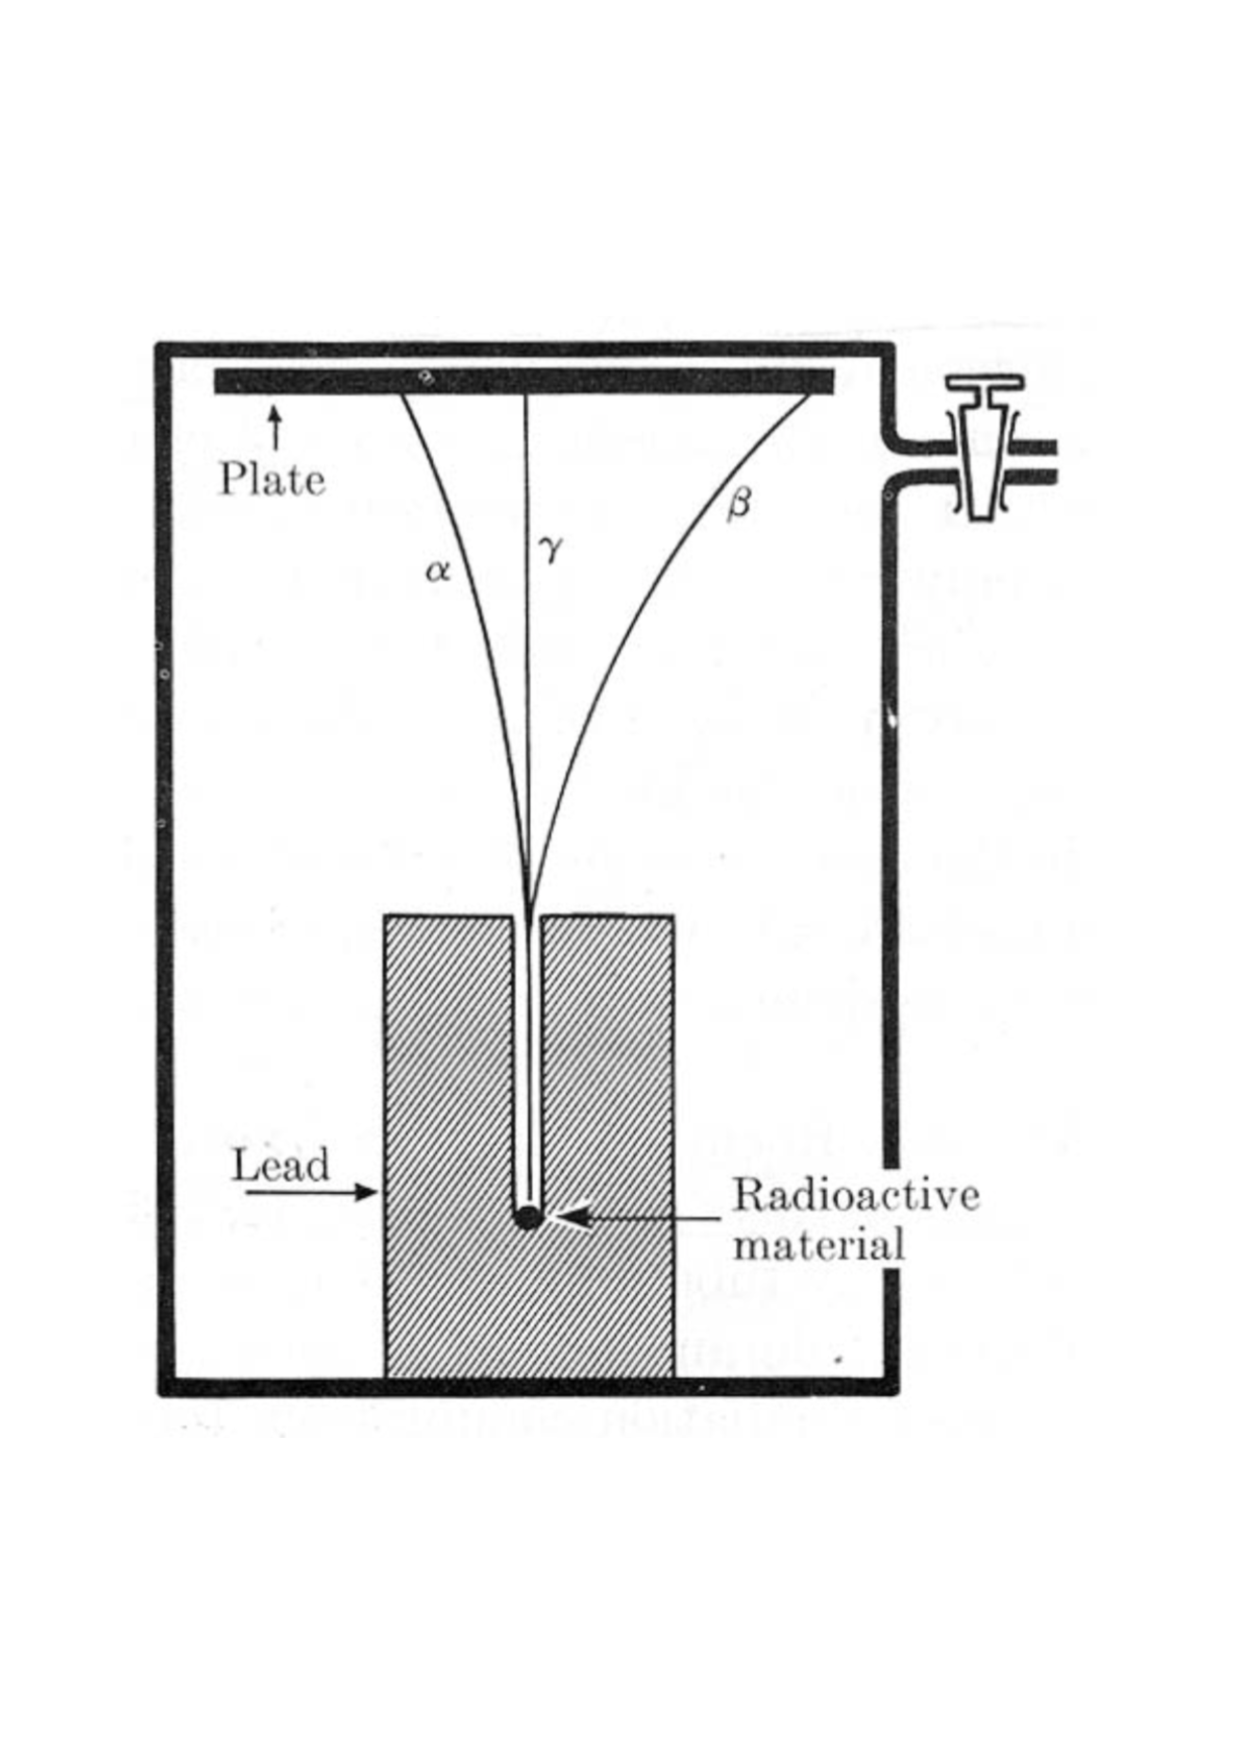
\includegraphics[width=.4\textwidth]{Becquerel}
    \caption{The device used by Ernest Rutherford.}
    \label{fig:Radioactivity}
\end{figure}

Different radioactive substances were placed in the device and the rays were either deflected in different directions or were not deflected. This showed that there were three types of radioactivity: one negatively charged, one positively charged and one neutral. The non-deflected neutral component was discovered in 1900, by the French physicist Paul Ulrich Villard. \\

By placing different absorbing materials in the path of radioactive rays, the different types of radiation could be characterized in terms of their penetrating power. The deflected types of radiations were named $\alpha$ and $\beta$, which were deviated in opposite directions by an external magnetic field. The neutral radiation was called $\gamma$. \\

In 1900, Becquerel verified that the ratio $e/m$ of the cathode rays experiment (described in Sec.~\ref{sec:ElectronDiscovery}) and that of the $\beta$ rays were identical: $\beta$ rays therefore seemed to be electrons. \\

In 1909, Rutherford identified the $\alpha$ rays as nuclei having a charge of $2e$, which were subsequently understood to be Helium $^4{\rm He}^{2+}$ ions. \\

\begin{table}[]
    \centering
    \begin{tabular}{llllll}
    \hline \hline
    Radiation    &  Nature  & mass & Energies & Spectrum & Penetration \\ \hline
    $\alpha$ & Helium ($^4{\rm He}^{2+}$) & 3.73~GeV & few MeV & Discrete & 6-7~cm \\ \hline
    $\beta-$ & Electron ($e^{-}$) & 0.511~MeV & from keV to MeV & Continuous & 5-7~m \\ \hline
        $\beta+$ & Positron ($e^{+}$) & 0.511~MeV& from keV to MeV & Discrete & 5-7~m \\ \hline
    $\gamma$ & Photon ($\gamma$) & 0 & from keV to MeV & Discrete & $\sim$~km \\ \hline
       $X$ & Photon ($\gamma$) & 0 & from $\sim$100~eV to keV & Discrete &  $\sim$~km \\ \hline \hline
    \end{tabular}
    \caption{Properties of the main forms of radiation: nature, mass, ranges of energies and penetration lengths.}
    \label{tab:Radioactivity}
\end{table}

\section{The discovery of the electron}
\label{sec:ElectronDiscovery}

It is interesting to note that while Crooks' tube was succesfully used to discover X rays, the nature of the initial beam was not fully known. The presence of something flowing from the cathode towards the anode in Crooks' tubes was known since 1876. This was understood by Eugene Goldstein who named them \emph{cathode rays}. The characterization of these rays came later from the development of cathode rays tubes (CRTs\footnote{The same technology used to build monitors and televisions until 2000s.}), which are vacuum tubes (as opposed to Crooks tubes, which were filled with tiny amounts of air).\\

It is in 1897 that Joseph John Thomson studied and discovered the nature of these electric charges. \\

\begin{framed}
\begin{experiment}[Discovery of the Electron - Joseph Thomson, 1897]
    
    The experiment conceived by Joseph Thomson used a cathode ray tube. The source of electrons can be simply a cathode, or they can be produced from a heated filament or from exposure to radiation. There is then an accelerating gradient to accelerate the cathode rays along the longitudinal ($x$) direction, see the Figure below:
    
        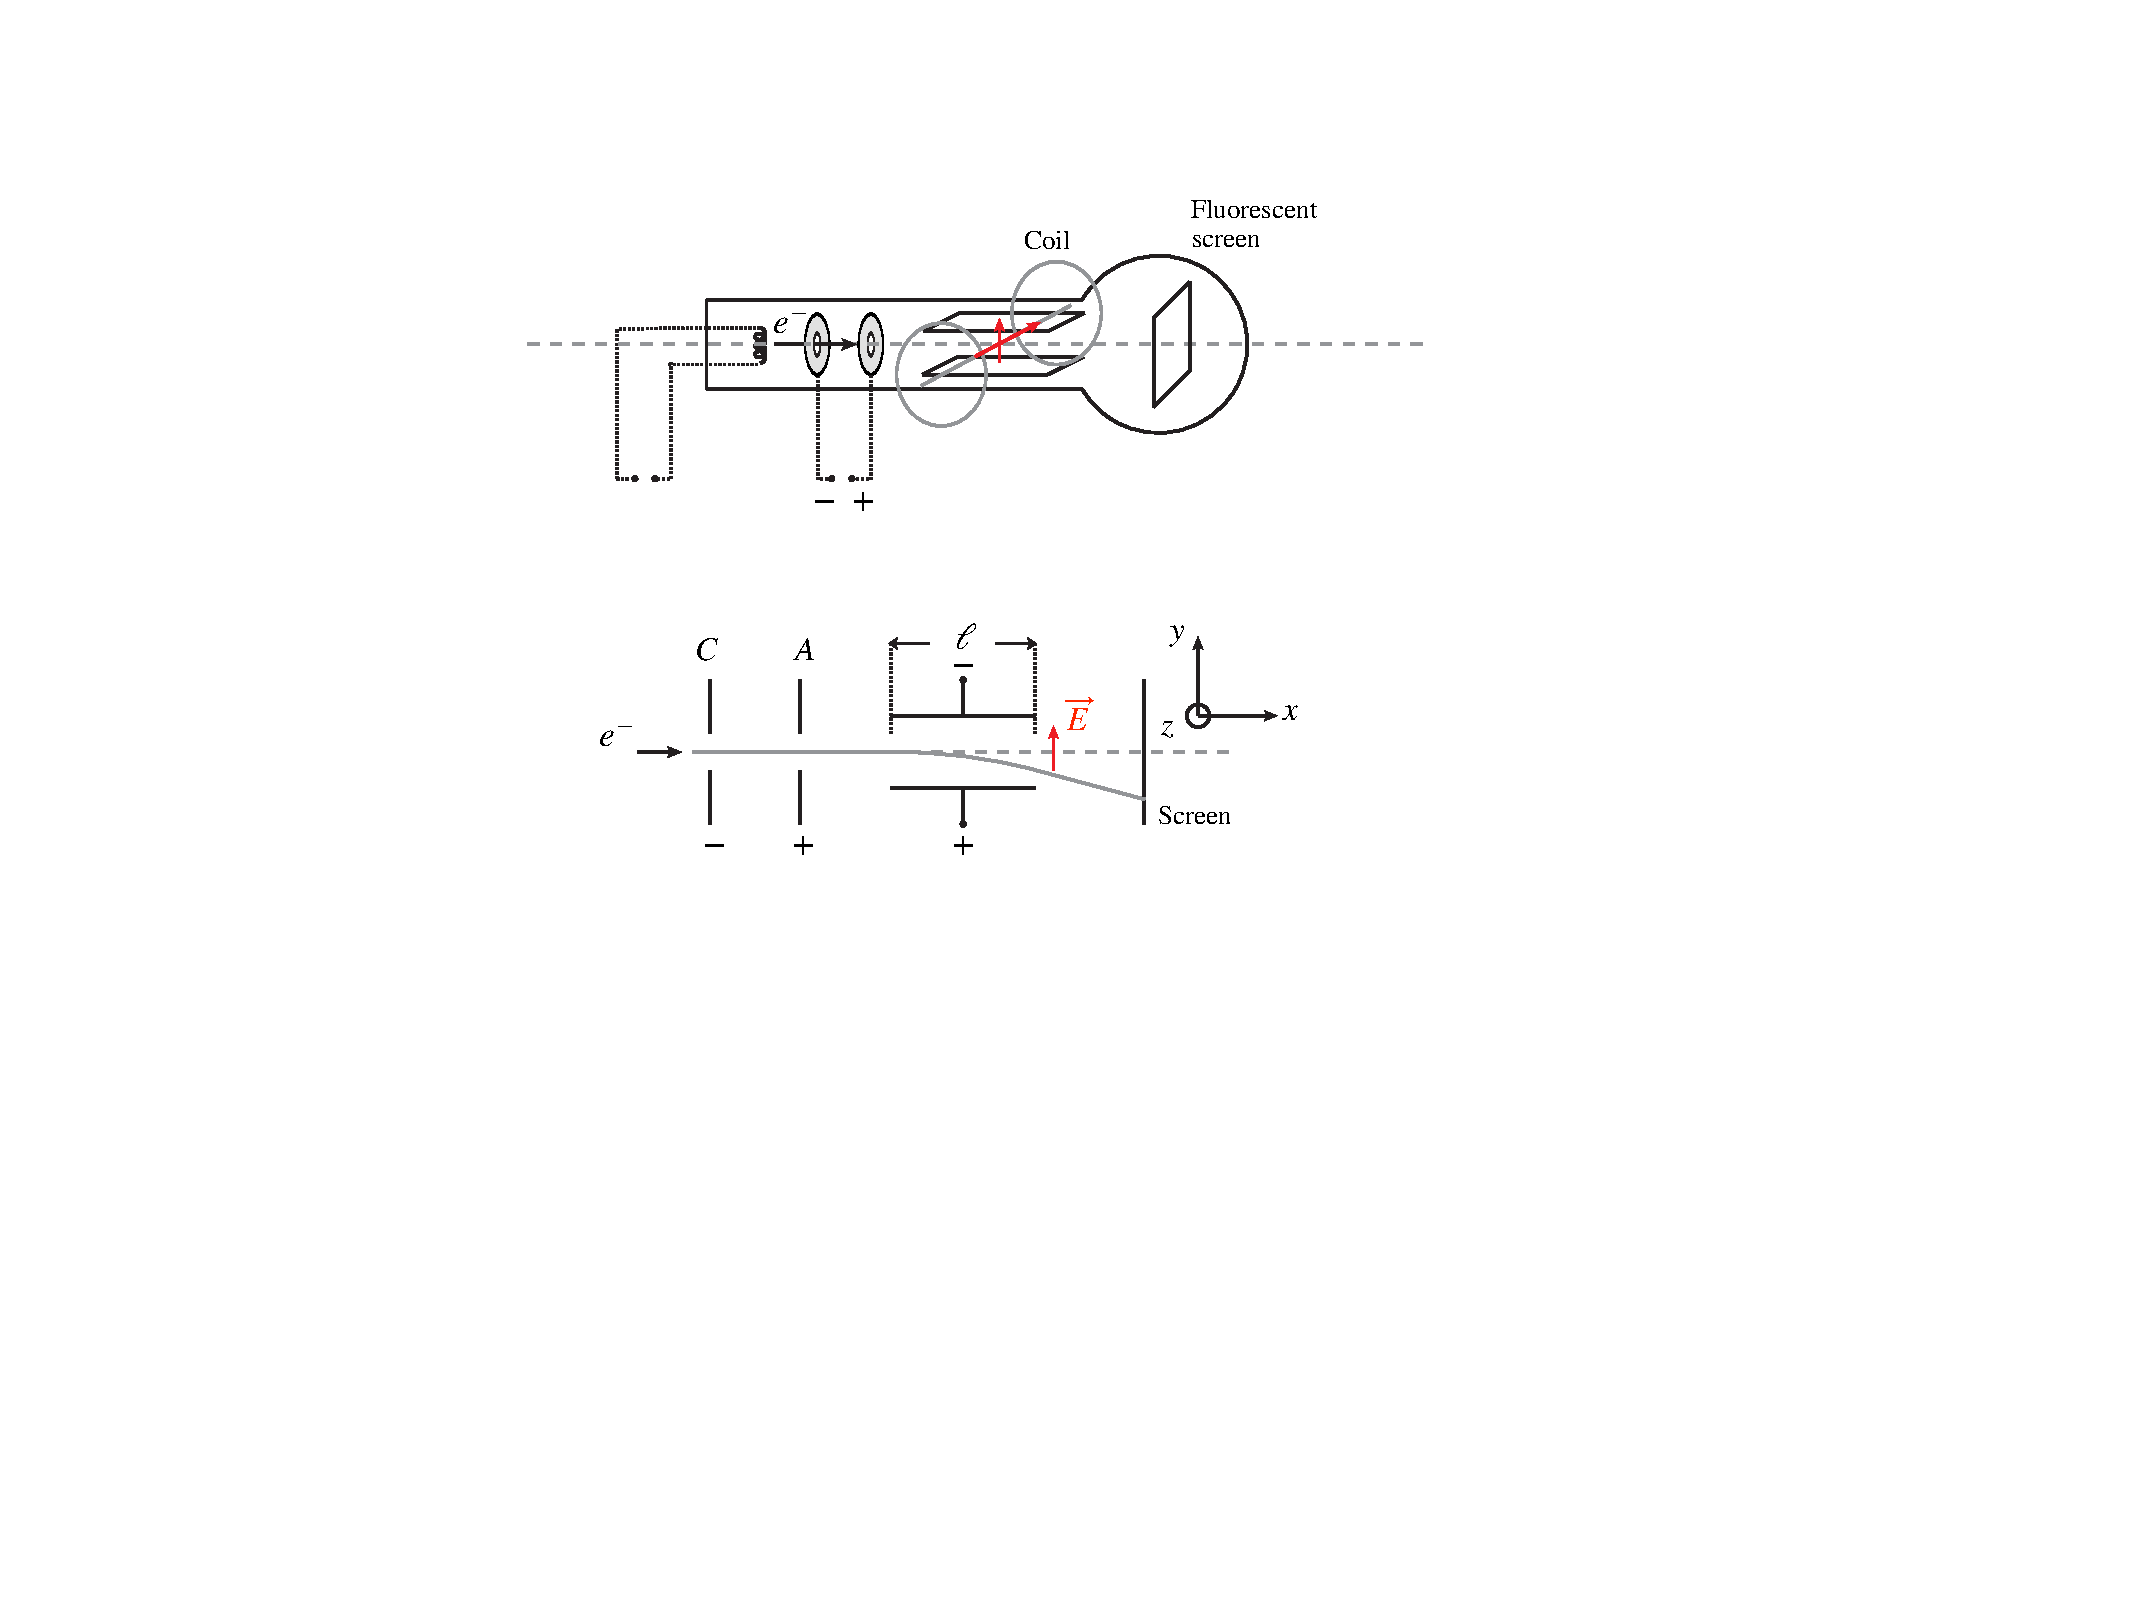
\includegraphics[width=.9\textwidth]{FNSN-Figure-1}

Once accelerated to a velocity $\vec{v} = (v_x, 0, 0)$, the beam passes through two horizontal plates generating an electric field $E$ along the $y$ direction, and coils producing a magnetic field $\vec{B}$ along the $z$ direction. The distance covered by the cathode ray between the plates is $\ell$, and the time passed through the plates is $\Delta t$ where:

$$ v_x = \frac{\ell}{\Delta t}.$$

In the presence of only the electric or only the magnetic field, the cathode rays are bent in the $y$ direction, thus showing that cathode rays are charged particles. The expected deviation of the rays can be computed assuming they are made of particles of mass $m$ and charge $q$: if we write $\vec{F} = q \vec{E} = m \vec{a}$, then

\begin{equation*} m \frac{dv}{dt} = q E \; \; \Rightarrow \; \; v = \int_0^{\Delta t} q \frac{E}{m} dt = q\frac{E}{m}\Delta t,\end{equation*}

and the vertical displacement can then be computed simply as

\begin{equation*}\Delta y = \int_0^{\Delta t} v dt  = \frac{1}{2}  q\frac{E}{m} \Delta t^2 = \frac{1}{2} q \frac{E}{m} \frac{\ell^2}{v_x^2} \end{equation*}

In order to determine the unknown $v_x$,  Thomson had the idea to apply a magnetic field $\vec{B}$ which could be controlled by the currents in the coils. The resulting force exerted on the cathode ray can then be expressed as

\begin{equation*}\vec{F} = q (\vec{E} + \vec{v} \wedge \vec{B}).\end{equation*}

Assuming that the region immersed in the magnetic field is the same as that covered by the electric field, varying the magnetic field in order to compensate perfectly the deviation of the electric field will then yield a measurement of the velocity $v_x$:

\begin{equation*} \vec{F} = \vec{0} \; \; \Rightarrow \; \; q(E - v_x . B) = 0,\end{equation*}

which yields the $v_x=\frac{B}{E}$.

From the measurement without the magnetic field, which yields $\Delta y$, and the measurement of the magnetic field needed to compensate the effect of the electric field, $B$, one can obtain a measurement of the ratio $q/m$:

$$ \frac{q}{m} = 2 \Delta y \frac{E}{\ell^2 B^2} $$

Thompson verified that $q/m$ did not depend neither on the gas in the tube, nor on the cathode material chosen. He therefore established the existence of a negatively charged particle, the electron.
    \end{experiment}    
     \end{framed}       

In his study of the deflection of the cathode rays under the combined effect of electric and magnetic fields, Thomson demonstrated that not only they were associated to negative electric charges: they were also made of particles with a definite relation between charge and mass. The denomination "electrons" was proposed by G. J. Stoneyin 1891 to describe these particles.\\

It is interesting to note that the charge to mass ratio for the cathode rays is much larger than the ratio of the elementary charge divided by the elementary mass, as determined in the case of Faraday's electrolysis experiments. This showed that there seem to be two types of components in the atom, with very different masses or very different charges. Assuming that the charges are the same (since the atom is electrically neutral, there had to be charges that mutually balance), the mass of the electrons had to be much lighter.\\

\section{The Zeeman effect}

Interestingly, during the same period as Thomson's discovery another striking discovery was made on a completely different subject: the impact of a magnetic field on the  emission of light. First intuitions on a possible effect were formulated by Faraday, but it wasn't until the works of Pieter Zeeman in 1896 that the effect was observed. Zeeman demonstrated that in the presence of a magnetic field the spectral lines of a light source show different components. This effect was first observed right before the discovery of the electron, and it allows to independently evaluate the charge-mass ratio $q/m$ of electrons. \\

The Zeeman effect can be described in a semi-classic fashion starting from the Bohr model of the atom, which will be described in more detail in Chapter~\ref{chap:InteractionsInMatter}. Considering a circular orbit of electrons with quantized angular momentum, for an electron with a velocity $v$ the electric current in the loop of the orbit of the electron will be given by

\begin{equation*} I = -\frac{e}{T}=-e \frac{v}{2 \pi r}, \end{equation*}
where $T$ is the period of the orbit and $r$ its radius.

\begin{figure}
  \centering
  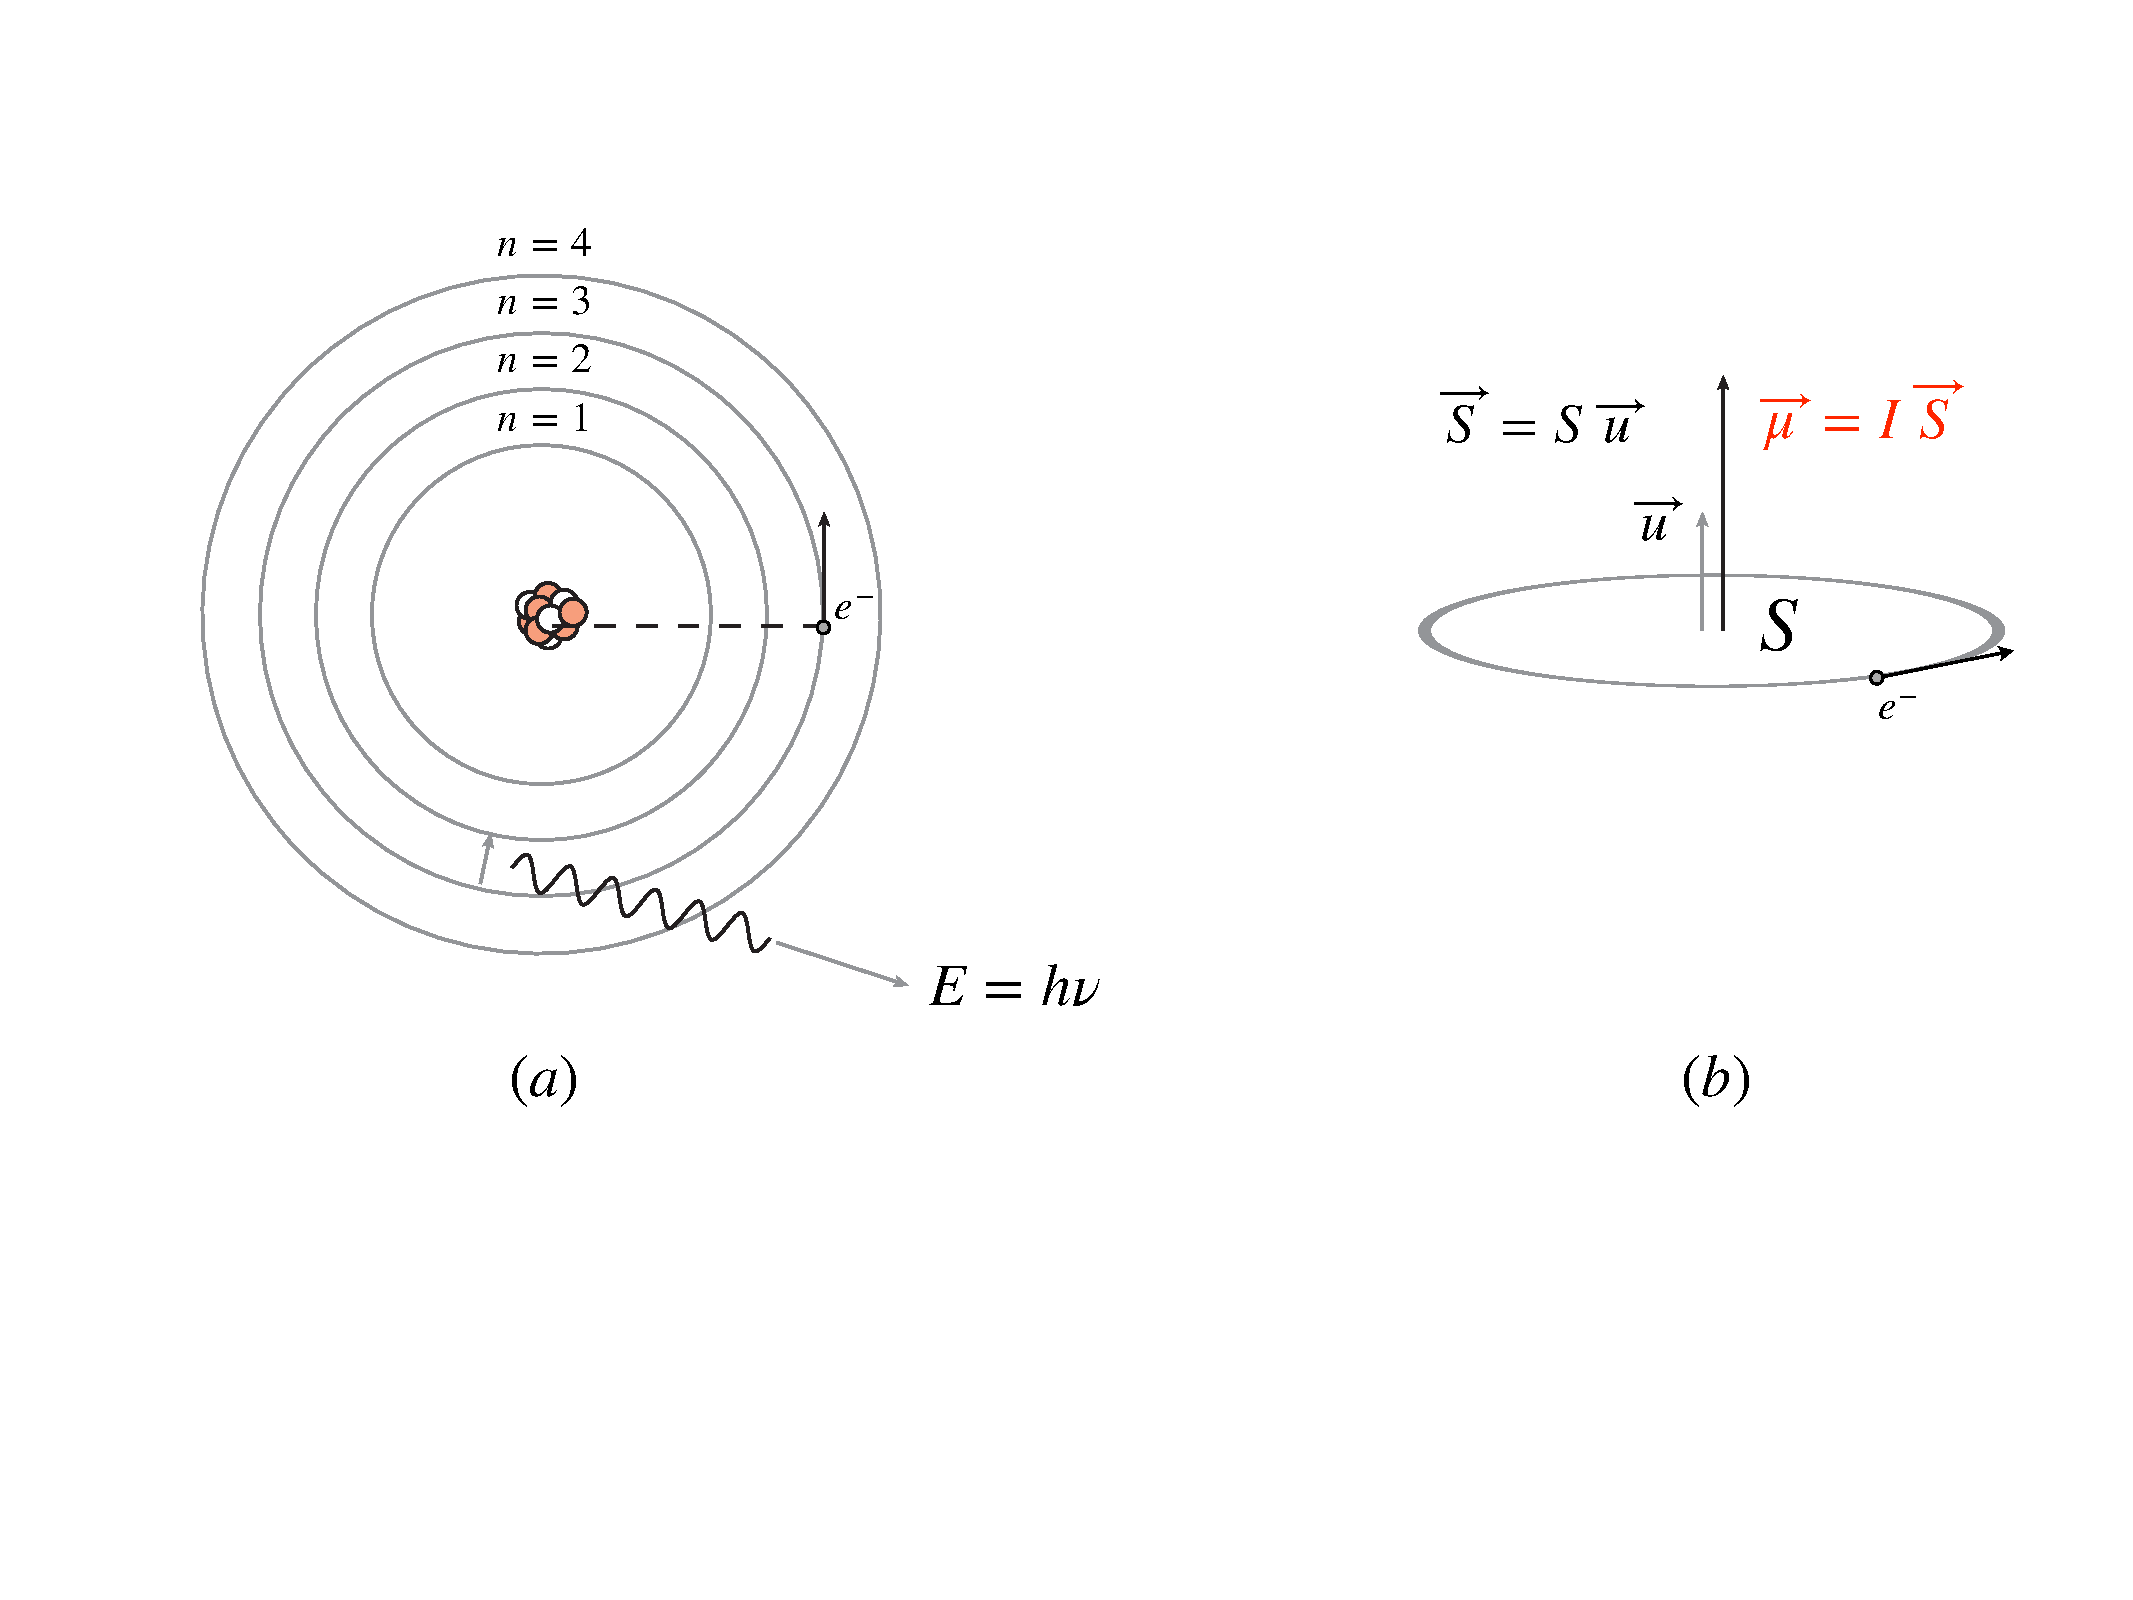
\includegraphics[width=0.8\textwidth]{Bohr}
\caption{Illustration of (a) the Bohr atomic model and (b) the magnetic moment created by the circular orbit of the electron.}  \label{fig:Bohr}
\end{figure}{}
 

The electric current of the orbit creates a magnetic moment (see Fig.~\ref{fig:Bohr}) $\vec{\mu}$:

\begin{equation*} \vec{\mu} = I \, \vec{S} = -e v \frac{r}{2} \vec{u}, \end{equation*}
where $S=\pi r^2$ is the surface of the circular orbit, and $\vec{u}$ the unit vector normal to this surface. The magnetic moment can then also be expressed in terms of angular momentum as:
\begin{equation*} \vec{\mu} = -\frac{e}{2 m_e} \vec{L}, \end{equation*}
where $\vec{L} = \vec{r} \wedge \vec{p} = m_e vr \vec{u}$ is the  angular momentum of the electron, and $m_e$ its mass. The quantization of the angular momentum is obtained by resolving the Schr\"odinger equation for the hydrogen atom: the eigenvalues of the operator $L^2$ are
\begin{equation*}L^2 = \ell (\ell +1) \hslash^2,\end{equation*}
where $\ell$ is the orbital quantum number.

If the atom is immersed in a magnetic field $\vec{B}$, the potential energy of the system will be given by
\begin{equation*} E = \vec{\mu} \cdot \vec{B} = \frac{e}{2 m_e} \vec{L} \cdot \vec{B}, \end{equation*}
where in the Bohr model the projections of $\vec{\ell}$ along the $z$ direction\footnote{Of course, the choice of the direction $z$ is arbitrary.} are $\ell_z = m_{\ell} \cdot \hslash$, where $m_{\ell}$ can take the values:
\begin{equation*} m_{\ell} \in \{ -\ell, -\ell+1, \dots \ell+1, \ell \}.\end{equation*}
In this case the orbitals are not degenerate anymore, but they are rather split. The magnitude of the splitting will yield a difference in energy (with respect to the degenerate line) of:
\begin{equation*} \Delta E = \frac{e}{2 m_e}m_{\ell} \hslash B = \mu_B m_{\ell} B,\end{equation*}
\noindent where $\mu_B = \frac{e \hslash}{2 m_e}$ is called \emph{Bohr magneton}, and depends on the ratio $e/m_e$.

By measuring displacement of spectral lines $\Delta E$ induced by the presence of the magnetic field, one can therefore measure the ratio between the charge and mass of the electron. Zeeman found the same value as in the case of the Thomson experiment:

$$ \frac{e}{m} \sim 1.76 \cdot 10^{11} C (Kg^{-1})$$

It is interesting to note that well before the discovery of the structure of atoms and the existence of nuclei, Zeeman demonstrated an effect, that would prove extremely important in probing the atomic model, once the theoretical understanding of the atom would have progressed sufficiently to describe it quantitatively.  \\

\section{The Millikan experiment and the Charge of the Electron}

The measurement of the charge -- and consequently the mass -- of the electron came later, with a very original experiment by Robert Millikan, in 1907. His experiment was based on  the study of fine oil droplets moving in air. The small drops were either charged by friction on the spout of the atomizer, or by using a X ray source.\\

\begin{figure}
    \centering
      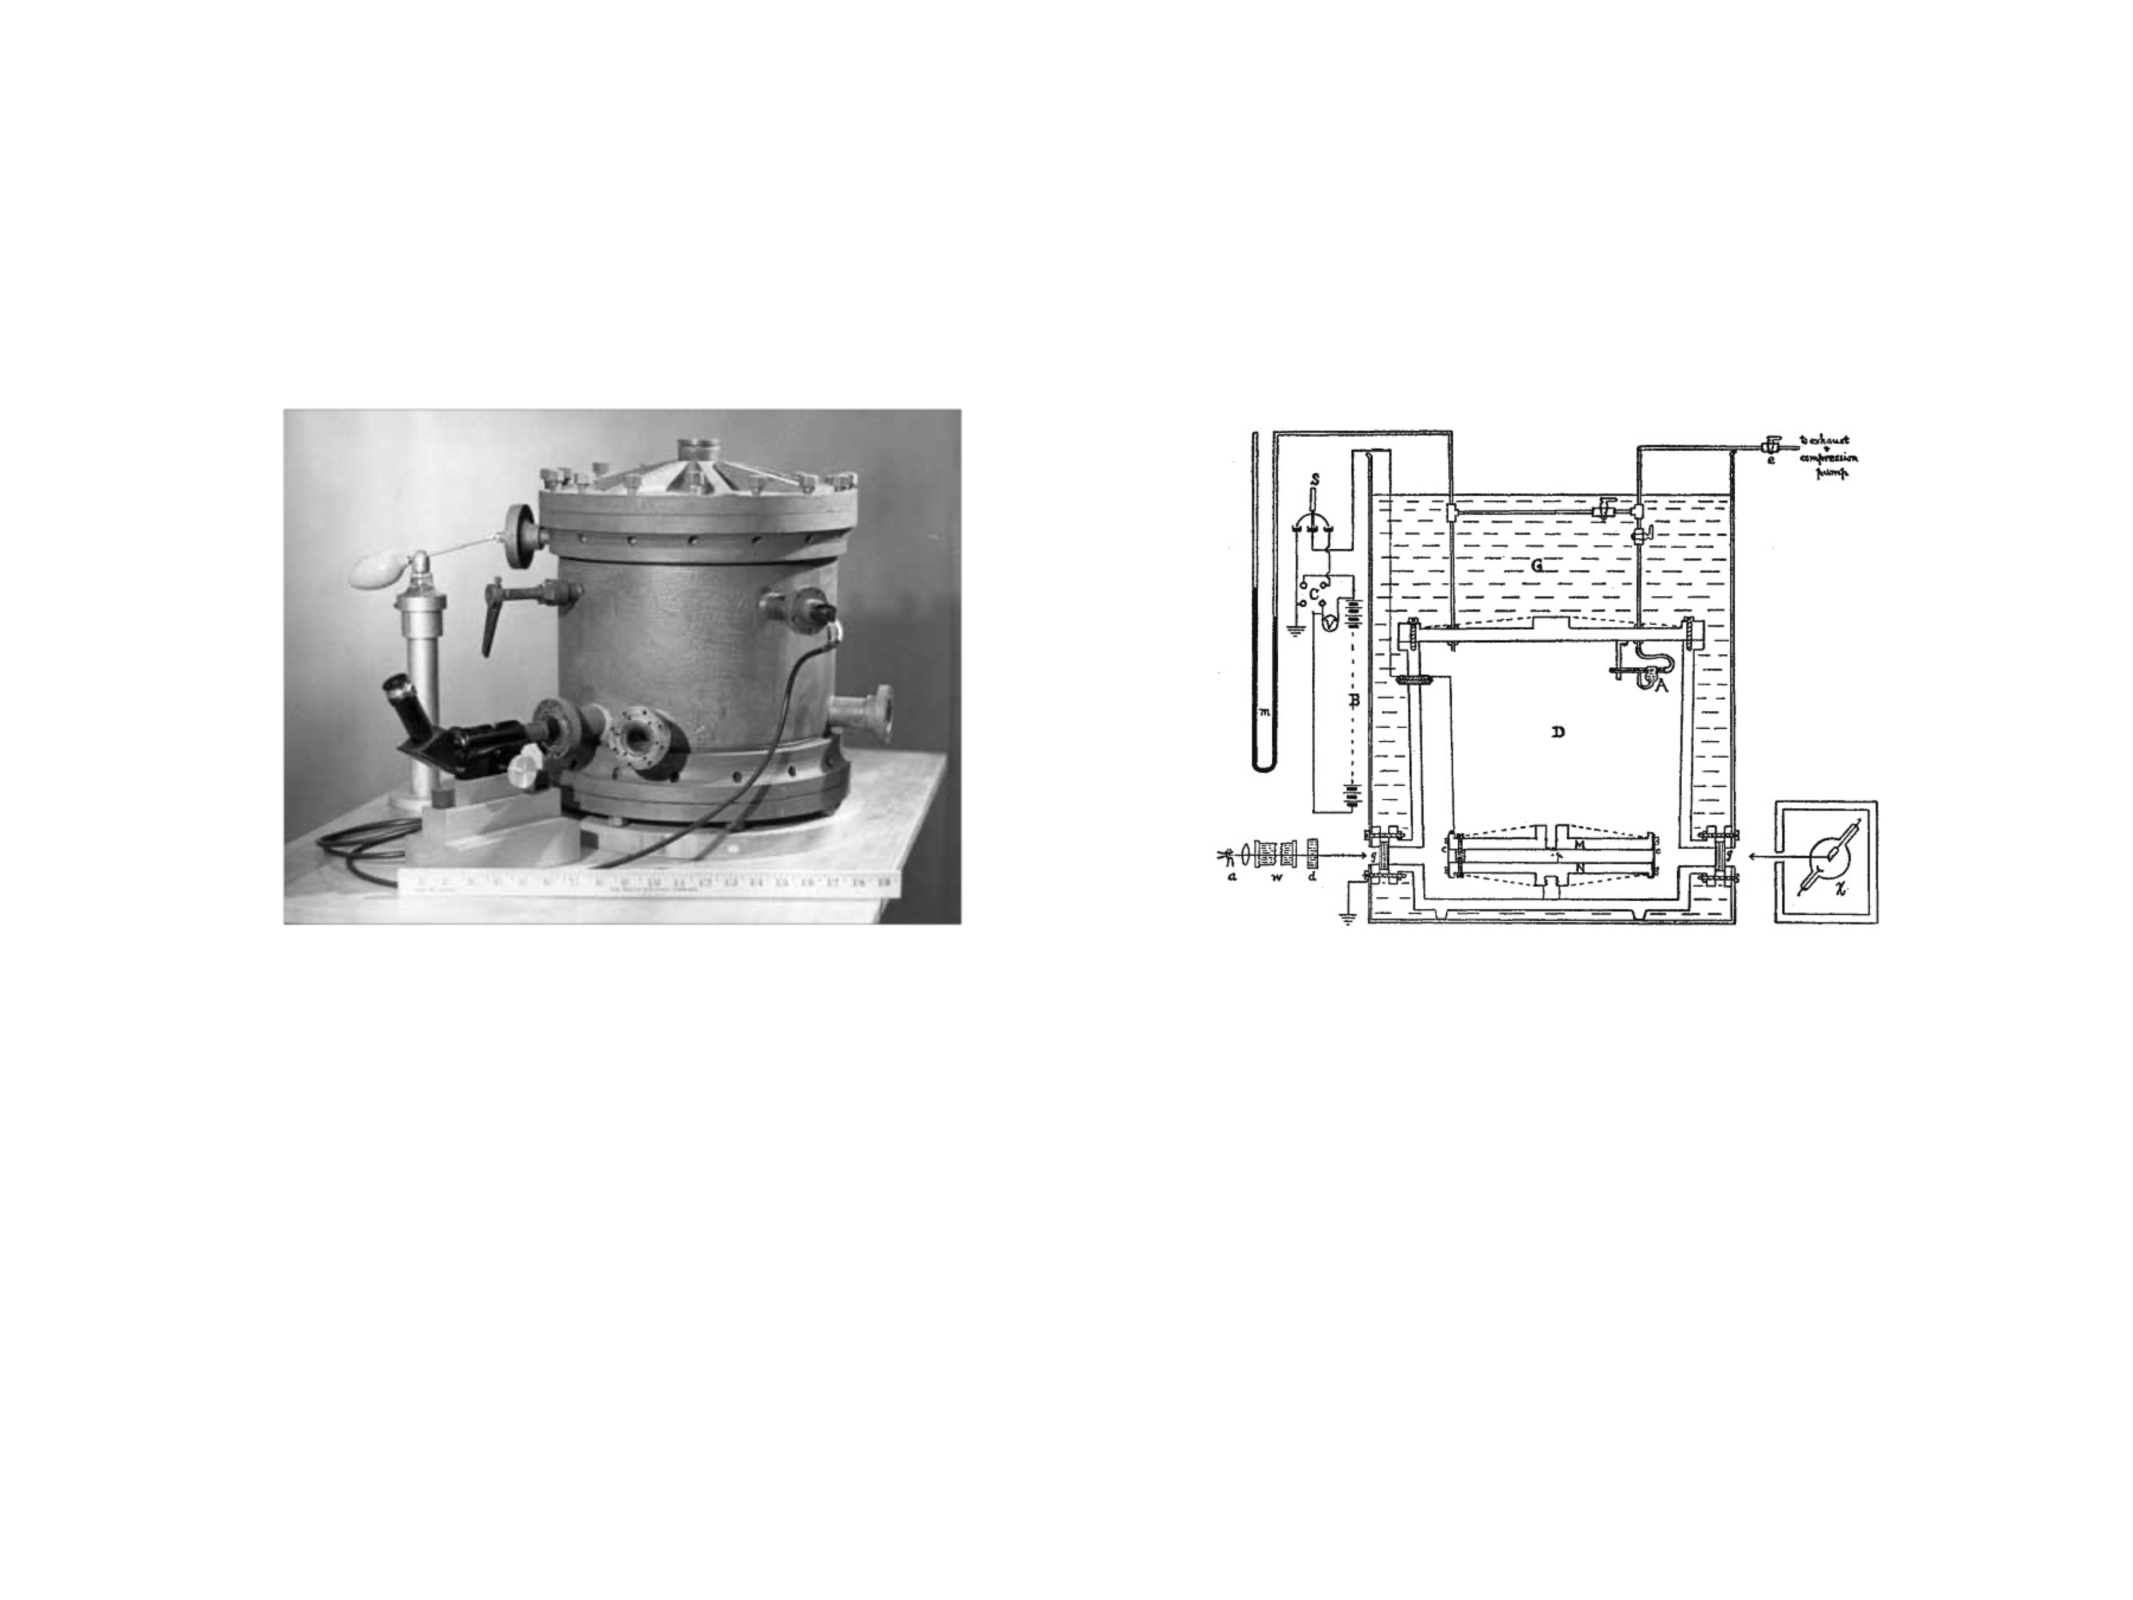
\includegraphics[width=1.0\textwidth]{Millikan}
    \caption{The Millikan experiment setup (left) and a schematic view from the original article (right). M and N represent the condenser plates, A designates the atomizer and in X the "R\"ontgen" (X ray) source is placed. The brass Vessel D is immersed in a gas-engine oil bath at constant temperature with fluctuations not larger than \SI{0.2}{\deg}.}
    \label{fig:Millikan}
\end{figure}

The setup of the experiment is illustrated in Fig.~\ref{fig:Millikan}. The movement of the spheric body in a fluid is subject to a frictional force proportional to the velocity ($v_0$) and to the radius ($r$) of the moving body. This is expressed by Stoke's law,
\begin{equation*}
     F = 6 \pi \eta r v_0,
\end{equation*}
where $\eta$ is the viscosity of the medium in which the body is moving. If we call the density of the moving body $\rho$, and consider that a droplet is -- to a good approximation -- a sphere, then its mass can be expressed in the following way:
\begin{equation*}M = \frac{4}{3} \pi r^3 \rho,\end{equation*}
where $\rho$ is the oil density. \\

The resultant buoyancy of the sphere due to Archimedes' principle in air, corresponding to the mass of air displaced by the volume of the droplet, is
\begin{equation*}M_a = \frac{4}{3} \pi r^3 \rho_a\end{equation*}
where $\rho_a$ is the density of air. Therefore, when the droplet reaches a uniform speed, all forces cancel yielding:
\[
\frac{4}{3} \pi r^3 (\rho-\rho_a) g = 6 \pi \eta r v_0.
\]
One can measure the velocity of individual drops by observing their fall through a microscope. Given the above formula, measuring $v_0$ gives the radius of the droplets:

$$ r^2 = \frac{9 \eta v_0}{2 g (\rho - \rho_a)}.$$

By applying an electric field in such a way that the electrostatic force is opposite to gravity, the force $qE$ will slow the fall down. The voltage applied is high enough to generate an electric field of approximately \SI{6000}{V/cm}. The voltage is then tuned in order to stop the motion of the droplets ($v = 0$), i.e.

$$ q \frac{V}{d} - Mg = 6 \pi \eta r v = 0.$$

Having previously measured the radius of the droplets was therefore essential to infer the mass of the droplets. This experiment yielded measurements of the elementary charge of the electron to be:
$$ e = 1.59 \cdot 10^{-19} \; \; {\rm C},$$
slightly smaller than the currently known value of $1.6 \cdot 10^{-19}$~C.\\

It is now known that Millikan's value was very slightly biased due to an error in the estimate of the viscosity. This insignificant mistake had a very interesting impact in understanding measurement biases and is often cited as such due to the fact that many subsequent experiments found values close to the one found by Millikan. The experiment is therefore often given as an example of non-conscious bias towards an already measured value. \\

From the measured ratio of $e/m$ the mass of the electron can be determined, yielding

\begin{center}
\fbox{
$m_e = 9.109 \cdot 10^{-31} \; {\rm kg} $,
}
\end{center}
which corresponds to $m_e c^2 = 0.511$~MeV in microscopic units as discussed in Chapter~\ref{chap:units}.


\section*{Take-home lessons}
\begin{itemize}
    \item Ancient atomism was surprisingly visionary in its (merely philosophical) attempt to describe nature. Empirical observations in Chemistry (e.g. Dalton's and Gay-Lussac's laws) built the foundations of modern atomism. Faraday's laws on electrolysis suggested the existence of unit charges and of the concept of elementary particle (then identified as the proton). The existence of atoms was proved later, with the explanation of brownian motion.
    \item Different kinds of radioactivity were discovered, and classified first based on their properties, and then based on our understanding of elementary particles. 
    \item $\beta^+$ radiation, consisting of electrons, was originally observed in the form of cathode rays.
    \item X rays were observed when sending electrons (cathode rays) on atoms: they were later understood to be photons which were either emitted by the electrons due to bremsstrahlung radiation (continuum spectrum due to the deflection of their path by the atomic nucleus), or photons emitted by an atomic electron which moved from an outer to an inner  level to replace another atomic electron kicked off by the cathode ray (discrete spectrum).
    \item Spontaneous emission of radioactivity by materials was later discovered and soon understood to be different from X rays. Radiation was classified as $\alpha$, $\beta$ and $\gamma$ depending on its deflection by magnetic fields. We now know that $\alpha$ particles are Helium nuclei ($^4He^{2+}$), $\beta^-$ radiation is made of electrons, $\beta^+$ of positrons (the electron anti-particle), and $\gamma$ and X rays are made of photons of different typical energies.
    \item Experiments helped measure the basic properties of particles. The electron charge-mass ratio could be measured (i) by altering the path of cathode rays using electric and magnetic fields, or (ii) with a measurement of the splitting of energy levels induced by the presence of magnetic field, as explained by the Zeeman effect in terms of the angular momentum and Bohr magneton of electrons.
    \item The charge of the electron could be measured by first charging small oil droplets (e.g. by friction or irradiation with X rays), and then using an electric field to stop their fall in air. 
\end{itemize}
\section*{Questions}
\begin{itemize}
    \item How many protons are there in a \si{kg} of carbon?
    \item Can you draw the $1s\to2p$ spectral line of hydrogen with and without magnetic field?
\end{itemize}
\begin{thebibliography}{99.}%

\bibitem{atomismeantique} Christian Gruber et Philippe-André Martin, de l'atome antique à l'atome quantique, \`a la recherche des mystères de la matière, presses polytechniques et universitaires romandes, EPFL, Lausanne (2013).

\bibitem{BrownianMotion} A. Einstein, \href{http://myweb.rz.uni-augsburg.de/~eckern/adp/history/einstein-papers/1905_17_549-560.pdf}{\"Uber die von der molekularkinetischen Theorie der W\"arme geforderte Bewegung von in ruhenden Fl\"ussigkeiten suspendierten Teilchen}, in Annalen der Physik, 17, 549–560, .

\end{thebibliography}
%%%%%%%%%%%%%%%%%%%%% chapter.tex %%%%%%%%%%%%%%%%%%%%%%%%%%%%%%%%%
%
% sample chapter
%
% Use this file as a template for your own input.
%
%%%%%%%%%%%%%%%%%%%%%%%% Springer-Verlag %%%%%%%%%%%%%%%%%%%%%%%%%%
%\motto{Use the template \emph{chapter.tex} to style the various elements of your chapter content.}
\chapter{Elements of Special Relativity}
\label{Relativity} % Always give \ unique label
% use \chaptermark{}
% to alter or adjust the chapter heading in the running 

\section{Introduction}

In 1905 Albert Einstein wrote four papers that would profoundly change physics. The first explained the photoelectric effect, the second was on the Brownian motion, the third stated special relativity and the fourth the equivalence between mass and energy. Each of them were groundbreaking on their own; together, they 
made 1905 be regarded as the {\it Annus Mirabilis} of physics. \\

In this chapter we will discuss the findings of the last two of the four remarkable papers~\cite{Relativity-1,Relativity-2}. As was discussed in Chapter~\ref{chap:Introduction}, special relativity is one of the main pillars of modern physics and in particular of nuclear, subnuclear and elementary particle physics.\\

The first paper was on {\it ``Zur Elektrodynamik bewegter K\"orper''} (``The electrodynamics of moving bodies'') received by {\it Annalen der Physik} on June 30. The second {\it ``Ist die Tr\"gheit eines K\"orpers von seinem Energieinhalt abh\"angig?''} (``Does the Inertia of a Body Depend Upon Its Energy Content?'') was received by the same journal on November 21. \\

\section{Galilean Relativity}

\begin{postulate}[Galilean Relativity]
  \label{postulate:galilean-relativity}
  The laws of mechanics are the same in all inertial reference frames.\\
\end{postulate}

\begin{definition}[Inertial Reference Frame]
  A reference frame in which the 1st law of motion holds exactly (a point-like body without forces acting on it either is still or is moving with constant velocity on a straight line.)
\end{definition}

Starting from the postulate of Galilean Relativity, as an immediate consequence, for an observer in an inertial reference frame it's impossible to determine whether the frame itself is moving or not. \\

\begin{figure}
  \centering
  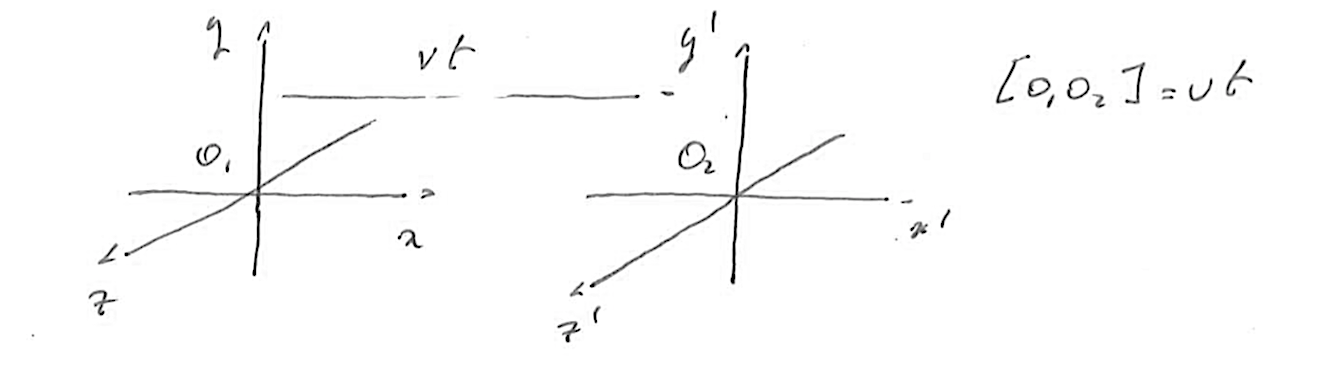
\includegraphics[width=\textwidth]{rel1}
  \caption{An example of an inertial frame $\mathcal{O}'$ moving with respect to another inertial frame $\mathcal{O}$ at constant velocity $v$.}
  \label{fig:rel1}
\end{figure}
A Galilean transformation allows to determine the relation between the coordinates of two inertial reference frames. With reference to Figure \ref{fig:rel1} the relations are the following:

\begin{equation}
  \begin{cases}
    &x = x' + vt\\
    &y = y'\\
    &z = z'\\
    &t = t'\\  
  \end{cases}
  \hspace{2cm}
  \begin{cases}
    x' = x - vt\\
    y' = y'\\
    z' = z\\
    t = t'\\  
  \end{cases}
\end{equation}

The fundamental point in these equations is that the coordinate changes only along the directions for which the components of $\vec{v}$ are different from $0$.\\

The diverging point from Galilean Relativity is an immediate consequence of Maxwell's equations. In fact, it can be easily proven that assuming the validity of Maxwell's equations implies that electromagnetic waves are moving at a constant velocity $c$, \\

\[c\simeq\SI{3e8}{m/s}.\]

At the time of the discovery of Maxwell's equations, physicists were not comfortable with the idea that light, and in general electromagnetic waves, are moving through the void. The common idea at the time was that light is moving through an invisible medium, which is uniformly distributed across the Universe: the \emph{Luminiferous Aether}, or ether. This idea predates modern electromagnetism, and was proposed very early by Christiaan Huygens in his {\it ``Treatise on Light''} in 1690, when he argued that light is a wave that propagates through aether. The concept of "aether" as a general way to explain interactions between bodies and the absence of vacuum was proposed by Robert Boyles a few years earlier. This idea, which was further developed through the years, wasn't fully satisfactory, as it required some sort of imperceptible material. When in the XIX century, with the development of electromagnetism, our knowledge of the nature of light progressed significantly, the existence of a Luminiferous Aether was being very strongly questioned. \\

\section{The Michelson-Morley Experiment}
In order to verify the existence of the Ether, Michelson and Morley developed a particularly sensitive experiment, whose layout is shown in Figure \ref{fig:rel2}. A light beam is produced by a source, and then split by a semi-reflecting mirror into two paths -- one parallel and one orthogonal to the velocity with which the experimental apparatus moves through aether (which is the speed of Earth).

\begin{figure}
  \centering
  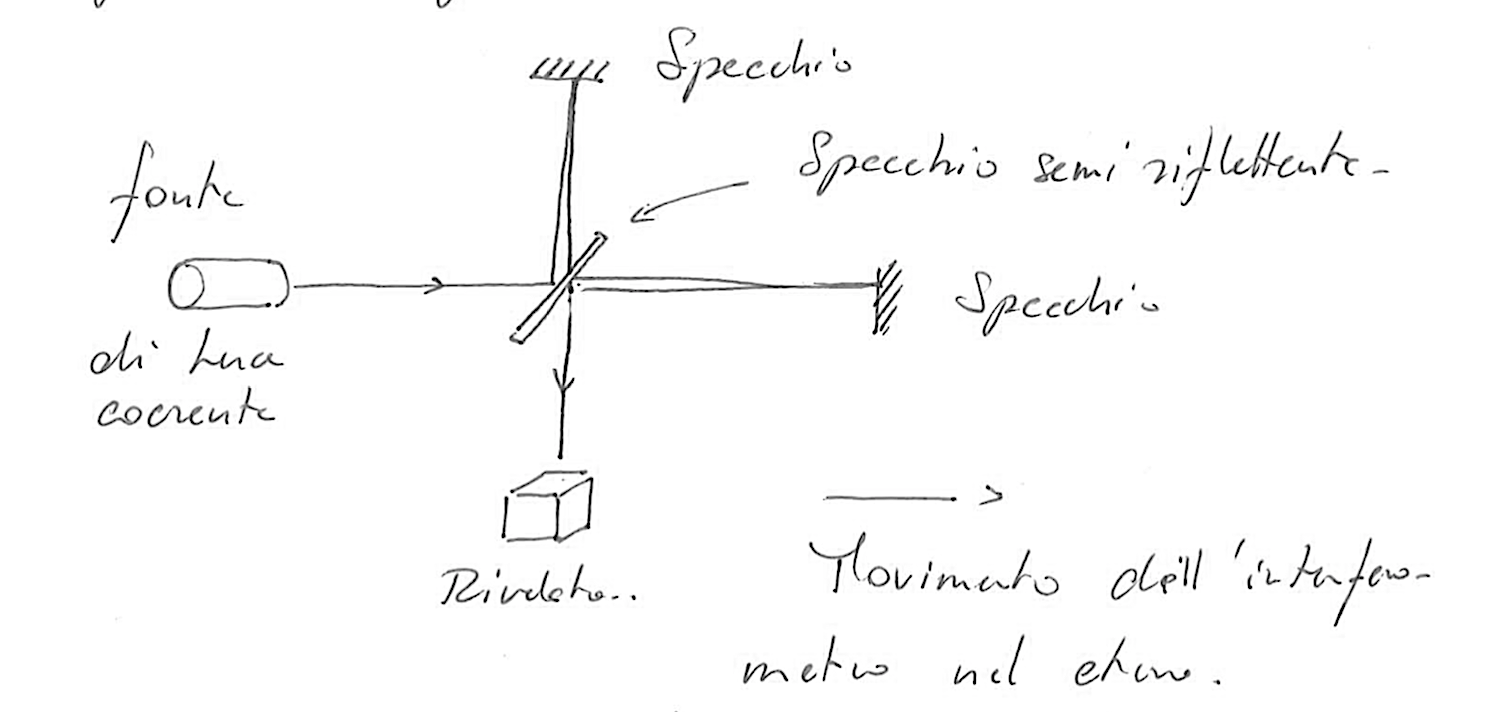
\includegraphics[width=0.8\textwidth]{rel2}
\caption{Layout of Michelson and Morley's experimental apparatus.}\label{fig:rel2}
\end{figure}{}

If the interferometer is moving through aether, then light (which is moving at $c$ with respect to the aether) will travel the distance of the two arms of the spectrometer in a different time, and a corresponding interference pattern will be produced between the two beams.\\

No such interference was visible with the Michelson and Morley experiment: light seemed to travel with the same speed over the two paths. It's only after this unexpected -- yet conclusive -- experimental result that physicists started to reject the idea of aether, accepting the fact that light travels at the same speed in all reference frames. \\

\section{From Simultaneity to Lorentz Transforms}
The theory of \emph{Special Relativity} is the theory which aims at describe space (and time) transformations between two inertial reference frames, one of which is moving with a constant velocity $\vec{v}$ with respect to the other.\\

The foundation of Special Relativity is on the following postulate, which is considered in addition to Postulate \ref{postulate:galilean-relativity}.

\begin{postulate}[Invariance of $c$]
  \label{postulate:invariance-of-c}
  The speed of light $c$ has the same value in all inertial reference frames. Its value is equal to
  \[c = \SI{299792458}{m/s}.\]
\end{postulate}

The theory of Special Relativity was built by Albert Einstein, starting from these two postulates, and exploiting more deeply the concept of \emph{Simultaneity}.
Einstein's definition of simultaneity follows from the following example. Consider two events which happen in two different points of the coordinate space: the two events can be considered as simultaneous if, after each one of them emits a light beam directed to the other event's position, an observer which is in the middle of them sees both the light beams at the same time.\\

\begin{figure}
  \centering
  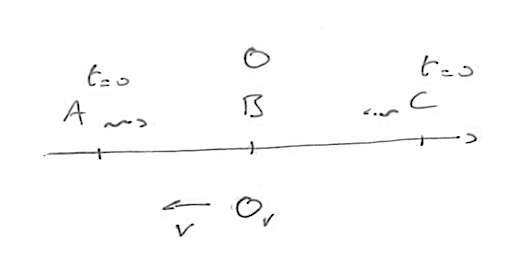
\includegraphics[width=0.8\textwidth]{rel3}
\caption{Graphic representation of simultaneity}  \label{fig:rel3}
\end{figure}{}

Let's make a more detailed overview of this example. With reference to figure \ref{fig:rel3}, an observer $O$ which is in $B$, whose position is fixed with respect to $A$ and $C$, will see the light from $A$ and $C$ simultaneously. Instead, an observer $O'$ which is moving with constant velocity $\vec{v}$ will see the light from $A$ before the light coming from $C$. In general, we have to take into account the fact that simultaneity depends on the reference frame!\\

Let's consider the example in a quantitative way: we want to find the coordinates of two events which are simultaneous by hypothesis (light beams from $A$ and $C$ reach the observer in $B$) in the moving reference frame $O'$. We call the space and time axes of $O'$ as $(x,t)$, which define the plane shown in Figure \ref{fig:rel4}: on this plane, the equation of motion of a light beam is a straight line with slope $t/x=1/c$ or $t/x=-1/c$ -- depending the direction along which it is emitted. The point $B$ lies on the same line as $A$ and $C$, at a distance $l$ from either. We call instead $(x', y')$ the coordinate system as measured by the observer in $O=B$.

\begin{figure}
  \centering
  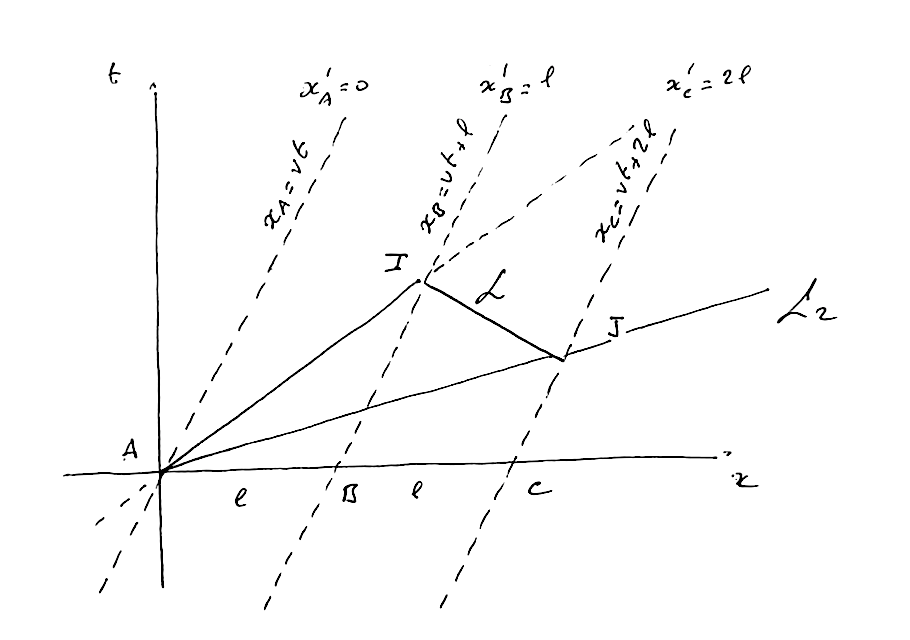
\includegraphics[width=0.8\textwidth]{rel4}
  \caption{In this figure, the coordinates $(x,t)$ belong to the reference frame of $O'$, which is moving at constant velocity $\vec{v}$ with respect to the points $A$, $B$ and $C$. Coordinates $(x',t')$ are the coordinates of the observer $O$, fixed with respect to $A$, $B$ and $C$.}  \label{fig:rel4}
\end{figure}

Let's compute the coordinates $(x_I,t_I)$ of the event $I$, ``Beam from $A$ arrives in $B$''. The point $A$ moves with constant speed $v$ with respect to $O'$, so the coordinates of $I$ will follow the equation of motion
\[x_I=vt_I+l.\]
But the beam moves with speed $c$, so
\[x_I=ct_I,\]
and hence
\[vt_I+l=ct_I,\]
which leads us to
\begin{align}
  t_I&=\frac{l}{c-v},\\
  x_I&=ct_I=\frac{cl}{c-v}.
\end{align}
In order for the event ``Beam from $A$ arrives in $B$'' to be simultaneous with the event ``Beam from $C$ arrives in $B$'', in the reference frame $O'(x,t)$ the second beam must have been emitted in point $J$, i.e. at a time $t_J\neq0$. This beam will travel in the direction of negative $x$, following the equation of motion
\[x=-ct+\alpha,\]
which corresponds to the line $\mathcal{L}$ on the $(x,t)$ plane of Fig. \ref{fig:rel4}; $\alpha$ is an unknown.
Since the second beam does reach the first beam in the intersection point $I$, then also the $I$ should satisfy the same equation,
\[x_I=\frac{cl}{c-v} = -\frac{cl}{c-v} + \alpha,\]
from which one has
\[\alpha = \frac{2cl}{c-v} = \frac{2l}{1-\frac{v}{c}},\]
and by defining
\begin{equation}
  \label{eq:beta}
  \beta = \frac{v}{c}
\end{equation}
we finally obtain
\begin{equation}
  \mathcal{L}:\ \ x=-ct+\frac{2l}{1-\beta}.
\end{equation}

The point $J$ has coordinates
\[
x_J = vt_J+2l,
\]
since it represents the position on the $(x,t)$ plane of the light source in $C=(l, 0)$ after a time $t_J$ has elapsed. It must also satisfy the equation for $\mathcal{L}$, so
\begin{align*}
  x_J = vt_J+2l &= -ct_J+\frac{2l}{1-\beta},\\
  \left[v+c\right]t_J &= 2l \left[\frac{1}{1-\beta}-1\right],\\
  c\left[1+\beta\right]t_J &= 2l \left[\frac{1-1+\beta}{1-\beta}\right],\\
  \left[1+\beta\right]t_J &= \frac{2l}{c} \left[\frac{\beta}{1-\beta}\right],\\
\end{align*}
which gives us
\begin{equation}
  t_J =\frac{2l}{c}\,\frac{\beta}{1-\beta^2},
\end{equation}
and
\begin{equation*}
    \begin{split}
  x_J &= vt_J+2l\\
  &= 2l \frac{\beta^2}{1-\beta^2} + 2l\,\frac{1-\beta^2}{1-\beta^2}\\
  &= 2l \frac{1}{1-\beta^2}\\
  &= \frac{c}{\beta}\,t_J,
  \end{split}
\end{equation*}
which is also the equation for the line $\mathcal{L}_2$. Each point on $\mathcal{L}_2$ corresponds to a simultaneous event.\\

The next task is then to derive the correct transformation laws which allow us to go from the coordinates $(x,t)$ to $(x',t')$. If $x = vt$ then the coordinate $x'$ should be zero (as $v$ is the speed of $O'(x,t)$ with respect to $O(x',t')$). This implies that
\[x' = f(v)\cdot(x-vt).\]

At this point it is important to note that events on the line $\mathcal{L}_2$ correspond to points that are \emph{simultaneous}. It is then explicit that {\bf simultaneity is frame dependent}. In the moving frame the events $A$ occurring at $t=0$ (see Fig.~\ref{fig:rel4}) and the event $J$ are not occurring at equal times, but \emph{they are simultaneous} from the Einstein light-ray definition of simultaneity. This also means that the time of event $J$ in the rest frame of the points $A$, $B$ and $C$ corresponds to $t'=0$. The line $\mathcal{L}_2$ therefore corresponds to $t'=0$.

For this reason, from the parametric form of $\mathcal{L}_2$, $t = xv/c^2 $, the following functional form is expected for $t'$:

\[t' = g(v)\cdot\left(t-\frac{v}{c^2}x\right)\]

Continuing on the {\it gedanken} experiment, let's suppose we consider a point along the the light ray emitted at $t=0$ at point A, whose spatial coordinates will therefore be $x=ct$. Since $A$ is part of $\mathcal{L}_2$, it also has $t'=0$, and since the light is assumed to be propagating at the same speed $c$ in any reference frame, then one has 
\begin{equation}
  \label{eq:B:1}
     x = ct \Rightarrow
    x'=ct'.
 \end{equation}
Using this necessary condition in the previous equations, we straightforwardly obtain that:
\begin{eqnarray*}
  x' &=& (x-vt)\cdot f(v) = (ct-vt)\cdot f(v)\\
  &=& t(c-v)\cdot f(v),\\
  t' &=& \left(t-\frac{v}{c}t\right)\cdot g(v)\\
  &=& \frac{1}{c} (c-v) t \cdot g(v)\\
  &=& \frac{1}{c} x' \frac{g(v)}{f(v)},
\end{eqnarray*}
from which one can deduce that the equation \eqref{eq:B:1} is satisfied if and only if:
\[g(v) = f(v).\]

To further derive the form of the coordinates transformations, another important {\it gedanken} step has to be taken. If the laws of physics are invariant in any inertial reference frame, then there is no difference in considering the expression of coordinates $(x',t')$ as function of $(x,t)$ or \emph{vice versa}. The expression of $(x,t)$ as function of $(x',t')$ should have the same functional form, but with an opposite velocity terms:

\begin{equation}
  \begin{cases}
    x = (x'+vt')f(v),\\
    t = \left(t' + \frac{v}{c^2}x\right)f(v),
  \end{cases}
\end{equation}
and substituting the expression for $x'$ one gets
\begin{eqnarray*}
  x &=& \left[ \left( x-vt\right)f(v)+\left(vt-\beta^2x\right)f(v)\right]f(v)\\
  &=& x\left[f(v)^2\left(1-\beta^2\right)\right].
\end{eqnarray*}
We can then define
\begin{equation}
  \label{eq:gamma}
  \gamma = f(v) = \frac{1}{\sqrt{1-\beta^2}},
\end{equation}
and express the Lorentz transformations as
\begin{eqnarray}
  x' &=& \frac{x-vt}{\sqrt{1-\frac{v^2}{c^2}}},\\
  t' &=& \frac{t-\frac{v}{c^2}x}{\sqrt{1-\frac{v^2}{c^2}}}.\\
\end{eqnarray}
or, using \eqref{eq:beta} and \eqref{eq:gamma}:
\begin{eqnarray}
  x' &=& \gamma x -\beta\gamma c t \\
  ct' &=& \gamma ct -\beta\gamma x
\end{eqnarray}
Note that $\beta\leq1$, $\gamma\geq1$

Note that in the limit $v/c \ll 1$ the Galilean expression of coordinate transformations is recovered. If we consider a Lorentz transformation in three dimensions, we can always make a rotation of the reference frame which brings our coordinate system with an axis ($x$ for example) parallel to $\vec{v}$. Then, the coordinates along axes which are orthogonal to the  direction of motion will not be affected by the transformation. 

The transformation can then be written as
\begin{equation}
  L(\beta)=
  \begin{bmatrix}
    ct'\\
    x'\\
    y'\\
    z'
  \end{bmatrix}
  =
  \begin{bmatrix}
    \gamma & -\beta\gamma & 0 & 0\\
    -\beta\gamma & \gamma & 0 & 0\\
    0 & 0 & 1 & 0\\
    0 & 0 & 0 & 1  
  \end{bmatrix}
  \begin{bmatrix}
    ct\\
    x\\
    y\\
    z
  \end{bmatrix},
\end{equation}

Note that the matrix is a symmetrical diagonalizable block matrix, and also:
\begin{equation}
  \det(L\left(\beta)\right) = \gamma^2 - \beta^2\gamma^2 = 1.
\end{equation}

As a simple consequence of the invariance of reference frames, the inverse matrix will be the one which describes the transformation from $(ct',x',y',z')$ coordinates to $(ct,x,y,z)$, i.e. the same matrix with a positive sign in front of $\beta$.

\begin{equation}
  L^{-1}(\beta)=
  \begin{bmatrix}
    \gamma & \beta\gamma & 0 & 0\\
    \beta\gamma & \gamma & 0 & 0\\
    0 & 0 & 1 & 0\\
    0 & 0 & 0 & 1  
  \end{bmatrix}.
\end{equation}

In the non-relativistic approximation it is common to consider the following expansion:
\begin{equation}
  \gamma = 1 + \frac{\beta^2}{2}+\mathcal{O}(\beta^2),
\end{equation}
which gives:
\begin{eqnarray*}
  x' &= & \gamma\left(x-\beta c t\right) = \left(1+\frac{\beta^2}{2}\right)\left(x-\beta c t\right)\\
  &= &x - \beta c t +\mathcal{O}(\beta^2),\\
  &\sim & x - vt,
\end{eqnarray*}
and
\begin{eqnarray*}
  t' &=& \gamma t -\frac{1}{c}\beta\gamma x \\
  &=& \left(1+\frac{\beta^2}{2}\right) t - \frac{\beta}{c}\left(1+\frac{\beta^2}{2}\right) x \\
  &=& t - \frac{\beta}{c}x +\mathcal{O}(\beta^2)\\
  &=& t - \frac{\beta^2}{v}x +\mathcal{O}(\beta^2)\\
  &\sim & t.
\end{eqnarray*}
As expected, we obtain Galilean transformations.\\

It is interesting to note that Lorentz transformations define a symmetry in 4-dimensional space. Other typical phenomena of Special Relativity can be derived from the structure of coordinate transformations.

\subsection{Contraction of lengths}
When we measure the length of an object, for example with a ruler, what we are measuring is the distance between its two endpoints, $A$ and $B$, i.e. we are measuring two positions. As the object may be moving with respect to us, we need to make sure we perform these two position measurements at the same time (in our reference frame).

\begin{figure}
  \centering
  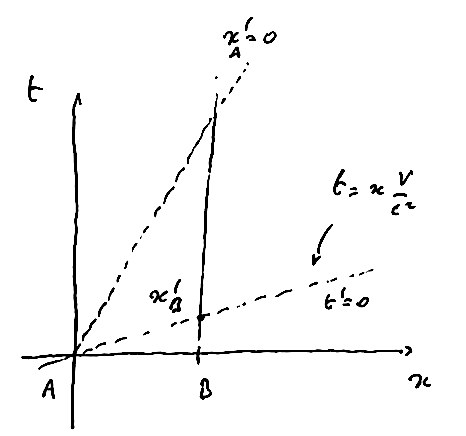
\includegraphics[width=0.8\textwidth]{rel5}
  \caption{Contraction of lengths between  two reference systems}
  \label{fig:rel5contraction}
\end{figure}{}

Figure~\ref{fig:rel5contraction} shows the position of the points $A$ and $B$ of an object in the reference frame $O(x,t)$. Since we have taken (with no loss of generality) $x_A=0$, the length of the object will be
\[L=x_B-x_A=x_B.\]
In the reference frame $O'(x',t')$, which moves with respect to $O$ with a speed $v=\beta c$, we will have
\begin{align*}
x'_A&=\gamma\left(x_A-vt_A\right) = -vt_A,\\
x'_B&=\gamma\left(x_B-vt_B\right).
\end{align*}
We perform the two measurements at the same time $t_A'=t_B'$, and we can take (with no loss of generality) $t_A'=0$. Therefore,
\begin{align*}
t_A&=\gamma(x_A\frac{v}{c^2}+t_A')=0,\\
t_B&=\gamma(x_B\frac{v}{c^2}+t_B') = \gamma x_B \frac{v}{c^2},
\end{align*}
and so
\begin{align*}
x'_A &= -vt_A=0,\\
x'_B &= \gamma x_B \left(1-\frac{v^2}{c^2}\right) = \gamma x_B (1-\beta^2)= x_B \frac{1}{\gamma} ,\\
\end{align*}
which leads to
\begin{equation}
  L' = x_B'-x_A'=\frac{L}{\gamma}.
\end{equation}
This means that the distance in the $O'$ frame is reduced by a factor $1/\gamma$. In a very similar way it is possible to compute that the distance measured by an observer in the $O$ frame is also reduced by the same factor.

\subsection{Time dilation}
Measuring time intervals in a given reference frame requires a clock to be put in a known, fixed position in that reference frame. For example, if we are at a Formula 1 race and we want to measure the distance between the events "first car reaches the finish line" and the event "second car reaches the finish line", we will place a clock at the finish line and read out its two measurements: their difference will be the desired time interval.

Let us consider the sketch in Fig. \ref{fig:rel6}. We are in the reference frame $O(x,t)$, and place a clock in point $A$ which (with no loss of generality) has $x=0$. We take a first time measurement $(x_1=0,t_1)$ (first car reaches $A$), and then another one $(x_2=,t_2)$ (second car reaches $A$). We have
\[
\Delta t = t_2 - t_1,
\]
and we want to measure $\Delta t'$ in a moving reference frame $O'$ (a third car).

\begin{figure}
  \centering
  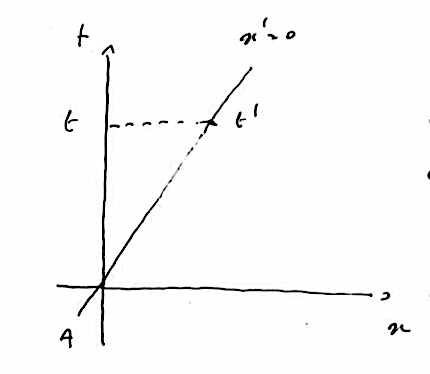
\includegraphics[width=0.8\textwidth]{rel6}
  \caption{Dilation of time between two reference systems}
    \label{fig:rel6}
\end{figure}{}

From the Lorentz transformations, we have
\begin{align*}
    t_1' = \gamma\left(t_1-\frac{\beta}{c}x_1\right),\\
    t_2' = \gamma\left(t_2-\frac{\beta}{c}x_2\right).\\
\end{align*}
The key point here is that the time measurement in $O$ must be performed keeping the clock in the same, fixed position $x_1=x_2$. Therefore, one gets immediately
\begin{equation}
  \Delta t' = \gamma \Delta t,
\end{equation}
a result known as \emph{time dilation}. In other words, the time interval between two events which happen at the same place in one reference system is always lower than measured by a moving reference frame. Note that this result is independent on the direction of velocity, and is the principle on which the so-called \emph{Twin Paradox} is built.\\

\subsection{Metrics}
Since the Lorentz transformations contract distances and dilate time intervals, one would expect the space-time distance to be preserved. Let's see if this is the case.

Consider a point $(x,t)$ and its Lorentz-transformed $(x',t')$:
\begin{align*}
  x' &= \gamma \left(x-\beta c t\right),\\
  t' &= \gamma \left(t-\frac{\beta}{c} x\right).
\end{align*}
By squaring both equations, we get
\begin{eqnarray*}
  x'^2 &=& \gamma^2 \left(x-\beta c t\right)^2\\
  &=& \gamma^2 \left(x^2 + \beta^2c^2t^2 -2\beta c x t\right),\\
  t'^2 &=& \gamma^2 \left(t-\frac{\beta}{c} x\right)^2\\
  &=& \gamma^2 \left(t^2+\frac{\beta^2}{c^2} x^2 -2\frac{\beta}{c}xt\right),\\
\end{eqnarray*}
so that
\begin{eqnarray*}
  (ct')^2&=& \gamma^2 \left((ct)^2+\beta^2 x^2 -2\beta x (ct)\right),\\
  x'^2  &=& \gamma^2 \left(x^2 + \beta^2(ct)^2 -2\beta x (ct)\right).\\
\end{eqnarray*}

It is clear that the distance $(x^2+t^2)$ does not work, because it's not conserved by Lorentz transformation. Instead, the distance defined as $(ct)^2 - x^2$ is conserved:
\begin{eqnarray*}
  (ct')^2 - x'^2 &=& \gamma^2\left[(ct)^2(1-\beta^2) + x^2(\beta^2 -1 ) \right]\\
  &=& \gamma^2 \left[(ct)^2-x^2\right](1-\beta^2)\\
  &=& (ct)^2 - x^2.\\
\end{eqnarray*}
The extension of this result to transformation with three components of velocity is trivial, where the distance $(ct)^2 - x^2 - y^2 -z^2$ is conserved. In other words, the following quantity is a relativistic invariant:
\begin{equation}
  \Delta s^2 = c^2 \Delta t^2 - \Delta x^2 - \Delta y^2 -\Delta z^2,
\end{equation}
or, better, in infinitesimal form:
\begin{equation}
  \dif{s}^2 = c^2 \dif{t}^2 - \dif{x}^2 - \dif{y}^2 -\dif{z}^2.
\end{equation}


\subsection{Proper time}
Consider again a clock which is moving together with an observer, as in Fig. \ref{fig:rel6}. In its reference frame $O'$, one has that $\dif{x}=\dif{y}=\dif{z}=0$ by construction (a reference frame is at rest with respect to itself). So we get
\[\dif{s}^2=c^2\dif{t}^2 - \dif{x}^2 - \dif{y}^2 - \dif{z}^2 = c^2 \dif{s}' = c^2 \dif{t}'^2\]
Thus, one can define the \emph{proper time}
\[
\dif{\tau} = \frac{\dif{s}}{c},
\]
which has the meaning to a metric measure of space-time, also called Minkowski space-time\footnote{You will appreciate the difference between Minkowski space-time and space-times which stem from different assumptions on how $\dif{s}$ depends on $\dif{x}, \dif{y}, \dif{z}, \dif{t}$ when studying general relativity.}.

\subsection{Light Cone}
Let us now consider the trajectory of a particle in space--time. In general, the trajectory of a particle always defines a time--like interval.
\begin{figure}
  \centering
  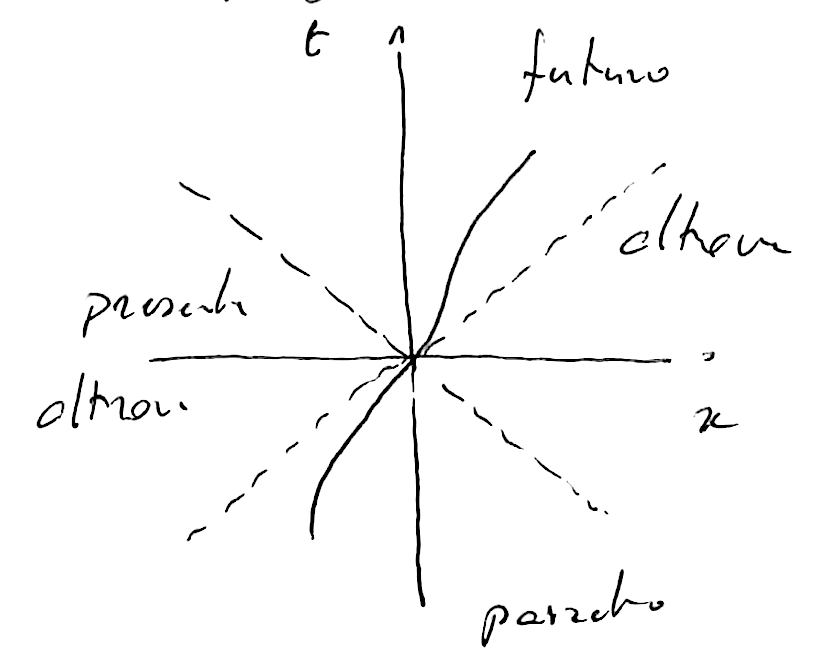
\includegraphics[width=0.5\textwidth]{rel7}
  \caption{Schematic representation of the light cone}\label{fig:rel7}
\end{figure}

\begin{definition}[Time--like interval]
  A time--like interval is a segment in space-time which satisfies:
  \[\dif{s}^2 = \left(c \dif {t}\right)^2 - \left(\dif{\vec{r}}\right)^2 > 0.\]
\end{definition}
For each time--like interval one can always write a corresponding Lorentz transformation for which $\dif{\vec{r}} = \vec{0}$, i.e. there is an inertial reference frame for which the two events are happening in the same place (at different times).

\begin{definition}[Space--like interval]
  A space--like interval is a segment in space-time which satisfies
  \[\dif{s}^2 = \left(c \dif{t}\right)^2 - \left(\dif{\vec{r}}\right)^2 < 0.\]
\end{definition}
In this case it's always possible to write a Lorentz transformation for which $\dif{t} = 0$, i.e. there is an inertial reference frame for which the two events are happening at the same time (in different places).\\

The space-time region in which $\dif {s}^2 = 0$ defines the \emph{light cone}. Events which are inside the light cone can belong to the past, present or future, and they can be connected with a time-like segment to the origin: in other words, they can be connected with a trajectory.

Events outside the light cone can be connected to the origin only with a space-like segment. This implies that a point outside the light cone can not be causally related.

\section{Four-vectors and covariant Notation}\label{sec:covariant1}
We have already introduced four--vectors: $(ct,x,y,z)$. Let's now introduce four-vectors with the superscript notation, which expresses each of its components in a short form:
\[x^\mu = \left(ct,x,y,z\right).\]

The position of the index (superscript or subscript) matters! The corresponding four-vector $x_\mu$ is defined as:
\[x_\mu = \left(ct,-x,-y,-z\right)\]

The action of ``moving the index from upper to lower position'' corresponds to the action of putting a minus sign in front of spatial coordinates. In other words, it corresponds to the multiplication of the four-vector by the \emph{metric tensor} $g^{\mu\nu}$, defined as\footnote{General relativity will show you why we took the disturb to use a tensor to describe operations, like computing $\dif{s}$, which are somehow simple: what here seems useless will prove crucial to deal elegantly with space-times more complex than the Minkowski space-time.}:
\begin{equation}
  g^{\mu\nu}=
  \begin{pmatrix}
    1 & 0 & 0 & 0  \\
    0 & -1 & 0 & 0  \\
    0 & 0 & -1 & 0  \\
    0 & 0 & 0 & -1  
  \end{pmatrix}.
\end{equation}
From this moment, we will also assume the convention of leave out sums on repeated indices: this is a common way to manipulate four-vectors also known as \emph{Einstein notation}. For example, the application of the tensor $g^{\mu\nu}$ to the four-vector $x_\nu$ can be written as:
\[x^{\mu} = \sum_{\nu=0}^3 g^{\mu\nu}x_\nu \equiv g^{\mu\nu}x_\nu.\]

Using the Einstein notation, the product between two four--vectors $U$ and $V$ can be written as:
\[U^\mu V_\nu = U^0V^0 - U^1V^1 - U^2V^2 - U^3V^3\]
and the Lorentz invariant $\Delta s^2$ can be written as:
\[\Delta s^2 = \Delta x^\mu \Delta x_\mu \]
Now, if we compute the differential of the four--vector $x^\mu = (ct, x, y, z)$, we obtain:
\begin{eqnarray*}
  \dif{x}^\mu &=& (c \dif{t}, \dif{x},\dif{y},\dif{z})\\
  \dif{s}^2 &=& \dif{x}^\mu \dif{x}_\mu
\end{eqnarray*}

As we have seen, proper time is defined as follows:
\begin{eqnarray*}
  d\tau^2 &=& \dif{t}^2 - \frac{1}{c^2}\left(\dif{x}^2+\dif{y}^2+\dif{z}^2\right),\\
  d\tau &=& \dif{t}\,\sqrt{ 1 - \frac{1}{c^2}\left(v_x^2+v_y^2+v_z^2\right)},\\
  d\tau &=& \dif{t}\,\sqrt{ 1 - \beta^2},\\
  d\tau &=& \frac{\dif{t}}{\gamma}.
\end{eqnarray*}

Velocity is clearly not invariant under Lorentz transformations, but we can  define the four-velocity as:
\begin{equation}  
u^\mu = \frac{\dif{x}^\mu}{d\tau},
\end{equation}  
which \emph{is} Lorentz-invariant.

It is a common convention to use $\mu$, $\nu$ and other Greek characters for indices running over the four components of four-vectors. To avoid errors, we will adopt the following two notational conventions, widely used in modern physics textbooks and literature:
\begin{itemize}
\item Four--vectors in space--time are denoted only and always with Greek indices, e.g. $x^\mu = (cx_0,x_1,x_2,x_3)$;\\
\item Three--vectors in three dimensional space are only and always written with latin indices, e.g. $x^j = (x_1,x_2,x_3)$.
\end{itemize}
This is equivalent to say that Greek indices range from $0$ to $3$, and latin ones from $1$ to $3$.

For example, we will denote velocity in space (three--vector) with:
\[\vec{v} = (v^1,v^2,v^3) = \left(\frac{\dif{x}_1}{\dif{t}},\frac{\dif{x}_2}{\dif{t}},\frac{\dif{x}_3}{\dif{t}}\right) \equiv v^i.\]

Following the definition of four-velocity:
\begin{eqnarray*}
  u^i &=& \frac{\dif{x}_i}{d\tau}\\
  &=& v_i\, \frac{\dif{t}}{d\tau},
\end{eqnarray*}
which allows us to write the common expression of four--velocity:
\begin{equation}
u^\mu = \gamma (c, \vec{v}),
\end{equation}
which highlights the definition of four-velocity as the proper-time derivative of a space-time four-vector. Although four-velocity is a four-vector, it has only three independent components due to the definition of $\gamma$, which immediately relates $u^0$ and $u^i$.

Motion and trajectories in space-time are defined in terms of $x^\mu$ and $u^\mu$, as illustrated in Fig. \ref{fig:rel8}.
\begin{figure}
  \centering
  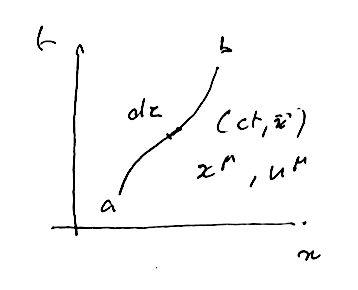
\includegraphics[width=0.5\textwidth]{rel8}
  \caption{Example of trajectory in a Minkowski space in terms of $x^\mu$ and $u^\mu$ }\label{fig:rel8}
\end{figure}

%\section{The Principle of Least Action in Non Relativistic Mechanics}

\section{Relativistic action and Hamiltonian of a particle}
To determine the dynamics of a system in this new relativistic framework a powerful starting point is the principle of least action, from which the Lagrangian and Hamiltonian describing the evolution of the system can be derived, as well as the equations of motion of a relativistic free particle. 

Action, as in classical mechanics, has to be constructed from the trajectory of a particle and {\it should} be invariant under Lorentz transformations. The latter condition ensures the principle of relativity, that the laws of physics are independent of the inertial reference frame we choose to describe them in. 

\begin{note}
The Galilean invariance of the action in Newtonian mechanics is not trivial, while it is straightforward from the fundamental principle of dynamics that Newtonian mechanics is invariant under Galilean transformations. Constructing the free particle action, both in the relativistic and Newtonian mechanics, imposing isotropy and homogeneity of space and time translation invariance of forces, the Lagrangian can only be a function of the square of the velocity of the particle, $\mathcal{L}(\vec{x},\vec{v},t) = \mathcal{L}(v^2)$. A Galilean transformation with a constant velocity $\vec{u}$ will transform $\vec{v} \rightarrow \vec{v} + \vec{u}$ and therefore $ v^2 \rightarrow v^2 + u^2 + 2\vec{v}.\vec{u}$. In this case it appears that if the Lagrangian is linear in $v^2$, then applying the Euler--Lagrange equations, the equations of motion will be invariant under a Galilean transformation. However, here the action is not explicitly invariant under Galilean transformations, but the equations of motion are. From this, it is also apparent that if the Lagrangian is not a linear function of $v^2$ then the equations of motion will not be invariant.
\end{note}

The only invariant we have built from the trajectory of a particle is the proper time (or proper length).
We can then postulate action of a free particle to be in the simplest form a function of the proper time:
\[S = \alpha \int_a^b d\tau,\]
where $\alpha$ is a constant factor that we will determine in a moment. Following the expression for $d\tau$ we get:
\[S = \alpha \int_a^b \dif{t} \sqrt{1-\frac{1}{c^2}\left(\dot{x}^2+\dot{y}^2+\dot{y}^2\right)},\]
where we denoted with a dot the derivative with respect to time.

Considering the action definition of Lagrangian Mechanics:
\[S = \int \dif{t} \mathcal{L},\]
we obtain that our candidate Lagrangian is
\[\mathcal{L} = \alpha \sqrt{1-\frac{1}{c^2}\left(\dot{x}^2+\dot{y}^2+\dot{y}^2\right)}.\]
In order to determine $\alpha$ we need to consider the approximation of the Lagrangian for small velocities, and equal it to the non-relativistic Lagrangian. For a slow particle, we have
\[\mathcal{L} \sim \alpha\left(1-\frac{v^2}{2c^2}\right).\]
Since $\mathcal{L}$ is invariant up to addition of constant terms (remember, $\alpha$ is constant), this is equivalent to
\[\mathcal{L} \sim -\alpha \frac{v^2}{2c^2},\]
and by comparison with the free--body Lagrangian in classical mechanics, which is equal to its kinetic energy $T$,
\[\mathcal{L} = T = \frac{1}{2}mv^2,\]
we reach the following choice of $\alpha$:
\[\alpha = -mc^2.\]

The relativistic free-particle Lagrangian can then be written as
\[\mathcal{L} = -mc^2\sqrt{1-\frac{1}{c^2}\left(\dot{x}^2+\dot{y}^2+\dot{z}^2\right)}.\]
From this point on, let's use coordinates $(x_1,x_2,x_3)$ to denote $(x,y,z)$ and simplify notation. According to the Euler--Lagrange equation, it is possible to obtain the three components of the spatial momentum of the particle by taking the derivatives
\begin{eqnarray}
  \label{eq:momentum}
  P_i &=& \frac{\partial \mathcal{L}}{\partial{\dot{x}_i}}\\
      &=& -mc^2\ \frac{\partial}{\partial{\dot{x}_i}}\sqrt{V\left(\dot{x}_i\right)},
\end{eqnarray}
where we used $V(\dot{x}_i)$ to represent the term under the square root. We obtain
\begin{eqnarray*}
  \dpar{}{\dot{x}_i}\sqrt{V(\dot{x}_i)} &=& \frac{1}{2\sqrt{V(\dot{x}_i)}}\dpar{V(\dot{x}_i)}{\dot{x}_i}\\
  &=& -\frac{1}{2\sqrt{V(\dot{x}_i)}}\frac{2}{c^2}\dot{x}_i.
\end{eqnarray*}

Therefore, the complete expression for $P_i$ is:
\begin{eqnarray*}
  P_i &=& \pd{\mathcal{L}}{\dot{x}_i} = -mc^2\,\frac{-\frac{1}{c^2}\,\dot{x}_i}{\sqrt{1-\frac{v^2}{c^2}}}\\
  &=& \gamma m \dot{x}_i,\\
\end{eqnarray*}
so that
\[
\vec{P}=m\gamma\vec{v}.
\]

Here the expression for the momentum of a free particle has been obtained, assuming only the definition of action, which satisfies the non--relativistic limit and the Euler--Lagrange equation. It is interesting to notice that (using Latin indices) the spatial components of $P$ can be written as function of the four-velocity:
\[P_i = m u_i.\]

Now we can derive the definition of energy, starting from the Hamiltonian, which is defined as a function of the generalised coordinates $q_i$ as
\[\mathcal{H} = \sum_i \dot{q}_i\dpar{\mathcal{L}}{\dot{q}_i} - \mathcal{L}.\]
In our case, this leads to the following expression:
\begin{eqnarray*}
  \mathcal{H} &=& \sum_{i=1}^3 \dot{x}_i p_i - \mathcal{L}\\
  &=& \sum_{i=1}^3 \gamma m \dot{x}_i^2 + mc^2\sqrt{1-\frac{v^2}{c^2}}\\
  &=& \gamma m v^2 + m c^2 \sqrt{1-\beta^2}\\
  &=& \gamma m v^2 + m c^2 \frac{1-\beta^2}{\sqrt{1-\beta^2}}\\
  &=& \gamma m v^2 + \gamma m c^2 \rr{1-\frac{v^2}{c^2}}\\
  &=& \gamma m c^2,
\end{eqnarray*}
and we have obtained the energy for a free particle:
\[E = \gamma m c^2.\]

Given the definition of four-velocity, $u^\mu = \gamma(c,\vec{v})$, we can observe that:
\[m u^0 = \frac{E}{c},\]
which allows us to write the four-momentum vector as
\[p^\mu = m u^\mu = \rr{\frac{E}{c},p^1, p^2, p^3}.\]

Now that we have a definition for energy, let's compute the norm of the four-velocity in terms of products of four-vectors:
\begin{eqnarray*}
  u^\mu u_\mu &=& \gamma^2\rr{c^2 - v_1^2 - v_2^2 - v_3^2}\\
  &=& c^2\gamma^2 \rr{1-\beta^2}\\
  &=& c^2,
\end{eqnarray*}
and multiplying by $m^2$ we get
\begin{eqnarray*}
  m^2 u^\mu u_\mu &=& (m u^\mu)(m u_\mu)\\
  &=& p^\mu p_\mu = m^2c^2.
\end{eqnarray*}
In another way:
\[p^2 = p^\mu p_\mu = \frac{E^2}{c^2} - p_1^2 - p_2^2 - p_3^2 = m^2 c ^2,\]
or, implying the sum on the index $i$,
\[\frac{E^2}{c^2} - \rr{p_i^2} = m^2 c ^2\]

It is important to note that the norm of the four-momentum only depends on the particle's mass: indeed, it is a Lorentz invariant.


\section{Noether's Theorem}
\label{sec:Noether1}
Noether's theorem has a crucial role in Particle Physics and in the calculus of variations.

\begin{theorem}[Noether's Theorem]
\label{TH:Noether}
To every continuous symmetry of the Lagrangian, i.e. to every continuous transformation of coordinates which does not change the Lagrangian, a corresponding conserved quantity is associated.
\end{theorem}

In order to give a clearer idea of this theorem, let's go through this example, which takes into account a possible symmetry of the free-particle Lagrangian we obtained in the previous section,
\[\mathcal{L} = -mc^2\sqrt{1-\frac{1}{c^2}\left(\dot{x}_1^2+\dot{x}_2^2+\dot{x}_3^2\right)}.\]
It is reasonable to assume that this Lagrangian should have the same functional form for particles that are located in different points of the space-time. In other words, this Lagrangian should be invariant under translation, a requirement which is written as

\begin{equation}
\label{eq:noether1}
\dpar{\mathcal{L}\rr{x^i,\dot{x}^i,t}}{x^i} = 0
\end{equation}

Now let's use the Euler--Lagrange equation, which is usually represented in terms of generalized coordinates as
\[\der{}{t}\rr{\dpar{\lag}{\dot{q}_i}}-\dpar{\lag}{q_i} = 0,\]
and can be written in our case as
\[\der{}{t}\rr{\dpar{\lag}{\dot{x}_i}}=\dpar{\lag}{x_i}.\]
This implies, taking into account equations \eqref{eq:momentum} and \eqref{eq:noether1},
\[\der{}{t}\rr{\dpar{\lag}{\dot{x}_i}} = \der{P_i}{t} = 0.\]
This means that the momentum is conserved under spatial translations. The statement of the theorem asks for a continuous coordinate transformation: this is needed to preserve the theorem for infinitesimal transformations, and to ensure that the derivative of \eqref{eq:noether1} exists.

A very similar computation can be easily done for translations in time.
By specifying that our Lagrangian  $\mathcal{L}\rr{x^i,\dot{x}^i,t}$ is dependent on three variables,  we can write its total time-derivative as:
\[\der{\lag}{t} = \dpar{\lag}{t}+\sum_i\qq{\dpar{\lag}{x_i}\dot{x}_i+\dpar{\lag}{\dot{x_i}}\ddot{x}_i}.\]
Again, using Euler--Lagrange equation on the third term, we have:
\begin{eqnarray*}
  \der{\lag}{t} &=& \dpar{\lag}{t}+\sum_i\qq{\rr{\der{}{t}\dpar{\lag}{\dot{x}_i}}\dot{x}_i+\dpar{\lag}{\dot{x_i}}\ddot{x}_i}\\
  &=& \dpar{\lag}{t}+\der{}{t}\sum_i\qq{\dpar{\lag}{\dot{x}_i}\dot{x_i}},\\
  -\dpar{\lag}{t} &=& - \der{\lag}{t} + \der{}{t}\sum_i\qq{\dpar{\lag}{\dot{x}_i}\dot{x_i}},\\
  \dpar{\lag}{t} &=& - \der{}{t}\qq{\sum_i\rr{\dpar{\lag}{\dot{x}_i}\dot{x_i}} - \lag},\\
  \dpar{\lag}{t} &=& - \der{\mathcal{H}}{t}.
\end{eqnarray*}
This gives another important conclusion: if the Lagrangian doesn't depend explicitly on the variable $t$, i.e. if $\pd{\lag}{t}=0$, then the Hamiltonian is constant, i.e. energy is conserved.

Since both of these conditions happen in our Lagrangian (invariance under space and time translations), the four-momentum is a conserved quantity.

%\section{Angular momentum}
%
%We will limit our discussion here to the case of spacial orbital angular momentum which is defined in a similar way as the non relativistic angular momentum as:

%$$ \vec{L} = \vec{p} \wedge \vec{r} $$

%{\bf \color{red} To be completed}

\section{Equation of motion and force}

It is finally interesting to connect these relativistic definitions with the more general notions of forces and the equation of motion. We start from a Lagrangian with a potential $V(\vec{x},\dot{\vec{x}},t)$,

\[ \lag = -\gamma(\dot{\vec{x}})mc^2 - V(\vec{x},\dot{\vec{x}},t).\]

Now, taking the Euler-Lagrange equation of motion,
\[ \der{}{t}\rr{\dpar{\lag}{\dot{\vec{x}}}}-\dpar{\lag}{\vec{x}} = 0 \]
with the above Lagrangian we get
\begin{eqnarray*}
\der{}{t}\rr{\dpar{\lag}{\dot{\vec{x}}}} & = &  \der{}{t} \rr{mc^2 \dfrac{2\dot{\vec{x}}}{2\sqrt{1-\dfrac{\dot{\vec{x}}^2}{c^2}}} - \dpar{V}{\dot{\vec{x}}}} \\
& = &
 \der{}{t} \rr{\gamma(\dot{\vec{x}})m \dot{\vec{x}} - \dpar{V}{\dot{\vec{x}}}},
\end{eqnarray*}
while the partial derivative is

\[\dpar{\lag}{\vec{x}} = - \dpar{V}{\vec{x}}.\]

Keeping the same definition of force as in Newton's second law of dynamics, i.e.
\[ \vec{F} = \der{\vec{p}}{t}, \]
one gets:
\[\vec{F} = \der{}{t} \rr{\gamma(\dot{\vec{x}})m \dot{\vec{x}}} = \der{}{t} \rr{\dpar{V}{\dot{\vec{x}}}} - \dpar{V}{\vec{x}}.\]

\section{More details on covariant notations}
In section \ref{sec:covariant1} we introduced the four-vector
formalism, defining two classes of four-vectors, those represented with
lower indices and upper indices:
\begin{itemize}
\item the components of a vector with upper indices, like $u^\mu$ or $u^i$,
  are called \emph{contravariant};
\item the components of a vector with lower indices, like $u_\mu$ or
  $u_i$, are called \emph{covariant}.
\end{itemize}

Why are these two representations of a vector different? A vector is an abstract object which can be
represented in a certain basis of linear--independent vectors,
\[\vec{v} = v^i \vec{e}_i\]
Of course, a new basis ${\vec{e}'_i}$ can be chosen and a
corresponding matrix $M^i_j$ is associated to the change of basis,
such that
\begin{equation}
  \label{eq:cova1}
  \vec{e}_j = M^i_j \vec{e}'_i
\end{equation}
This requires that $M$ is an invertible matrix, which means $\det(M) = 1$. In
addition to this, the components of the vector $\vec{v}$ are affected
by the following transformation:
\[\vec{v} = v^j \vec{e}_j = v^j M^i_j \vec{e}'_i,\]
where one should remember that we are implying sum on repeated indices, and that any element of
this equation like $v_j$ or $M^i_j$ should be treated as a
number. This means that, as long as indices are correctly written, the
commutative property holds between these elements, i.e.
\[v^j M^i_j \vec{e}'_i = M^i_j v^j \vec{e}'_i = v'^i \vec{e}'_i.\] This
defines\footnote{Note that we re-label the index $i$ into index $j$, as the name of the index is irrelevant as long as summation is implied.} the components $v'^j$ of the vector $\vec{v}$ represented in
the basis ${\vec{e}'_j}$,
\[v'^i = M^i_j v^j.\] The components of the vector under the new
basis are on the left side of the equation, and are obtained by
applying the matrix $M$ to the vector represented in the old
basis. This is the opposite as in equation \eqref{eq:cova1}: for this
reason the components of a vector, if represented with upper indices,
are called contravariant.

We have already defined the scalar product between two vectors, but in
a more general way we could say that
\begin{eqnarray*}
  \vec{v}\cdot\vec{w} &=& v^i\vec{e}_i \cdot w^j \vec{e}_j \\
                      &=& v^i w^j \vec{e}_i \cdot \vec{e}_j\\
                      &=& v^i w^j g_{ij},
\end{eqnarray*}
which defines also the metric tensor $g_{ij}$.

Now that we have a rule for the scalar product, the covariant
components of a vector can be defined as the projections of that
vector on the given basis,
\[v_i = \vec{v} \cdot \vec{e}_i, \] which implies the following rule:
\[v_i = v^j \vec{e}_j\cdot\vec{e_i} = v^j g_{ij}.\] The metric tensor
allows to change from covariant to controvariant components, and vice-versa.  If we
now apply the rule for the change of basis, we get
\begin{eqnarray*}
  v_i &=& \vec{v}\cdot\vec{e}_i\\
      &=& \vec{v}\cdot M^j_i \vec{e}'_j\\
      &=& M^j_i v'_j.
\end{eqnarray*}
Here the components $v_i$ are obtained applying the matrix $M$ to the
components in the new basis ($v'_j$), as done in equation
\eqref{eq:cova1}. For this reason, these components are called covariant.

In an Euclidean space, the metric tensor is the Kronecker's Delta
\[g_{ij} = \delta{ij}.\] This means that covariant and contravariant
components of a vector are identical. In general, and in the case of
Special Relativity, this is not true and the distinction between
covariant and contravariant components of a vector must be considered.

The metric tensor of the Minkowski space is
\begin{equation}
  g^{\mu\nu}=
  \begin{pmatrix}
    1 & 0 & 0 & 0  \\
    0 & -1 & 0 & 0  \\
    0 & 0 & -1 & 0  \\
    0 & 0 & 0 & -1
  \end{pmatrix}.
\end{equation}

An explicit way to represent contravariant and covariant components of a vector is
by using respectively column--like and row--like vectors. For example,
in euclidean space:
\begin{eqnarray*}
  u^i &=& \begin{pmatrix}
    u_1\\
    u_2\\
    u_3\\
  \end{pmatrix},\\
  u_i &=& \rr{u_1,u_2,u_3},
\end{eqnarray*}
and the scalar product can be written as
\[ u_iu^i =\rr{u_1,u_2,u_3} \begin{pmatrix}
    u_1\\
    u_2\\
    u_3\\
  \end{pmatrix}.\] This depends on the metrics! In the Minkowski space, in fact, one has
\begin{eqnarray*}
  u^\mu &=& \begin{pmatrix}
    u_0\\
    u_1\\
    u_2\\
    u_3\\
  \end{pmatrix},\\
  u_\mu &=& \rr{u_0,-u_1,-u_2,-u_3},
\end{eqnarray*}
and the scalar product is
\[ u_\mu u^\mu =\rr{u_0,-u_1,-u_2,-u_3} \begin{pmatrix}
    u_0\\
    u_1\\
    u_2\\
    u_3\\
  \end{pmatrix}.\]

\section*{Take-home lessons}
\begin{itemize}
    \item Special relativity extends Galilean relativity with the postulate of the universality of the speed of light.
    \item Simultaneity of two events, in special relativity, depends on the reference frame of the observer.
    \item Lorentz transformations can be obtained by the requirement that the laws of physics are invariant in any inertial reference frame, with the constraint that the speed of light is the same in every reference frame.
    \item Lengths contract by a factor $1/\gamma$ when measured in a moving reference frame.
    \item Time intervals dilate by a factor $\gamma$ when measured in a moving reference frame. In particular, time dilation is independent on the direction of velocity.
    \item The space-time of Special Relativity, also known as Minkowski space-time, is defined by a diagonal metric tensor, and by the proper length $\dif{s}=\dif{t}^2-\dif{x}^2-\dif{y}^2-\dif{z}^2$, or equivalently by the proper time $\dif{\tau}=\dif{s}/c$.
    \item The light cone defines time-like ($\dif{s}^2>0$), space-like ($\dif{s}^2<0$) and light-like ($\dif{s}^2=0$) intervals (or four-vectors). Intervals between causally-connected events are represented by time-like intervals. Time/space/light-likeness is a Lorentz-invariant property.
    \item Four-vectors have covariant and contravariant representations.
    \item Four-velocity transforms as a four-vector, while ordinary velocity isn't. 
    \item The energy-momentum-mass relation $E=\sqrt{mc^2+p^2c^2}$ follows from the relativistic action and Hamiltonian of a free particle, which in turn is obtained from the requirement of action to be Lorentz-invariant (and so expressed as a function of $\dif{\tau}$) and by comparing the low-speed limit of the Lagrangian with its classical expression. Momentum follows from Euler-Lagrange equation, while energy follows from the Hamiltonian.
    \item The conservation of energy and momentum is a consequence of the invariance of the free-particle Lagrangian under space and time translations. This is due to Noether's theorem, according to which each continuous symmetry of the Lagrangian corresponds to an associated conserved quantity. Another consequence of this is the conservation of angular momentum, which follows from rotational invariance.
    \item In the more general case of a free particle under some external potential, the force acting on it is expressed as a function of the derivatives (in time, space and velocity) of the potential, following the Euler-Lagrange equation.
\end{itemize}
\section*{Questions}
\begin{itemize}
    \item Where does the sign in the temporal component of the first equation of the Galilean and Lorentz transformations come from?
    \item Work out the Michelson-Morley's calculation for the time difference between the two light paths, in the assumption of Galilean mechanics. 
    \item How do volumes transform under Lorentz transformations? What about densities?
    \item Is momentum a space-like, a time-like or a light-like four-vector? What about four-velocity?
    \item Work out the transformation laws for three-velocity.
    \item Had we defined $\dif{s}^2=-c\dif{t}^2+\dif{x}^2+\dif{y}^2+\dif{z}^2$, would any conclusion of this chapter have changed?
\end{itemize}


%%% Local Variables:
%%% mode: latex
%%% TeX-master: "../book"
%%% End:

%  LocalWords:  Springer

\begin{thebibliography}{99.}%

\bibitem{Relativity-1} A. Einstein, Zur Elektrodynamik bewegter Körper in Annalen der Physik 17 (1905), pp. 891–921 \href{http://myweb.rz.uni-augsburg.de/~eckern/adp/history/einstein-papers/1905_17_891-921.pdf}{View article (PDF)}. 

\bibitem{Relativity-2} A. Einstein, Ist die Tr\"agheit eines K\"orpers von seinem Energieinhalt abh\"angig?, in Annalen der Physik, 18, 639–641, \href{http://myweb.rz.uni-augsburg.de/~eckern/adp/history/einstein-papers/1905_18_639-641.pdf}{View article (PDF)}.

\end{thebibliography}

%%%%%%%%%%%%%%%%%%%%% chapter.tex %%%%%%%%%%%%%%%%%%%%%%%%%%%%%%%%%
%
% sample chapter
%
% Use this file as a template for your own input.
%
%%%%%%%%%%%%%%%%%%%%%%%% Springer-Verlag %%%%%%%%%%%%%%%%%%%%%%%%%%
%\motto{Use the template \emph{chapter.tex} to style the various elements of your chapter content.}
\chapter{Elements of Scattering Theory}
\label{Scattering-1} % Always give a unique label
% use \chaptermark{}
% to alter or adjust the chapter heading in the running head

\section{Introduction}

Scattering is an overarching theme in modern physics. It is particularly essential in nuclear and sub-nuclear physics and has been by far the most important tool in the development of the field of nuclear and particle physics.

To reveal the structure and properties of matter, of fundamental particles and their interactions; the usual protocol is to hurl a beam of probe waves (sound or electromagnetic) or particles (X or $\gamma$ photons, electrons, protons, neutrons, alpha (helium ions, heavy nuclei ions, etc \ldots) and analyse the patterns of the scattered probes. Most of the current knowledge in atomic, nuclear and particle physics is based on scattering experiments and their interpretation. 

The term \emph{scattering processes} in these lectures will denote all processes where particles $A,B,C, \cdots$ in the initial state will interact to give particles $\Delta, \Sigma, \Xi, \cdots$ in the final state,

$$ A+B+C+ \cdots \rightarrow \Delta + \Sigma + \Xi +\cdots$$

\definition{{\bf Elastic scattering} denotes the scattering processes where the number of particles of each type is unchanged and only the direction and energy of the single particles is modified,
\[ A+B+C+ \cdots \rightarrow A + B + C +\cdots\]
In elastic scattering processes, the total kinetic energy for each is conserved.}

\emph{Scattering theory} is the mathematical framework that describes scattering processes. Through given hypotheses on the nature of the target, one can calculate the expected scattering predictions and compare them with the observed scattering pattern, thus testing the validity of those hypotheses.

The origin of scattering theory can be traced back to the kinetic theory of gases and the birth of statistical mechanics, with the work of Ludwig Boltzmann. There are two fundamental reasons why statistical elements enter the mathematical description of scattering. The first is practical: while the trajectory of an individual molecule or particle interacting in a given potential (or with another molecule or particle) could be calculated and measured, it is in practice impossible to describe precisely the ensemble of molecules or particles interacting with another ensemble of molecules or particles -- and a thermodynamic description of the ensemble of molecules is necessary. The second is the underlying probabilistic nature of quantum processes. 

\section{The classical hard spheres case}

We will start with a very simple classical example to immediately clarify the idea and the main ingredients of scattering theory. Let's take the simple example of two macroscopic objects interacting via a simple mechanical collision process, as the simple case of the elastic collision of two  spheres. In this macroscopic case we can know precisely the initial trajectory of the {\it "probe"} sphere ($A$, with radius $r$) (see Figure~\ref{fig:spheres}) and the relative position of the  {\it "target"} sphere ($B$, with radius $R$). In this simple picture, from the relative position of the two spheres -- which can be measured in terms of the {\it "impact parameter"} of the collision, i.e. the distance between the centers of two spheres -- scattering angle $\theta$ at which the probe sphere is scattered is fully determined. It is a {\it deterministic} process. In the case of hard spheres, the scattering angle can be easily derived from the impact parameter, given that the scattering angle with respect to the perpendicular to the tangent plane at the point of impact $\alpha$, will be equal to the impact angle (see Figure~\ref{fig:spheres}). In formulas, we have
\[ b = (R+r) \sin \alpha,\]
and the scattering angle $\theta$ will be related to $\alpha$ by $\pi = 2\alpha + \theta$ or $\alpha = \frac{\pi}{2} - \frac{\theta}{2}$, and thus
\begin{equation}
\label{eq:spheres}
\cos \frac{\theta}{2} = \frac{b}{R+r}.
\end{equation}

\begin{figure}
%    \centering
    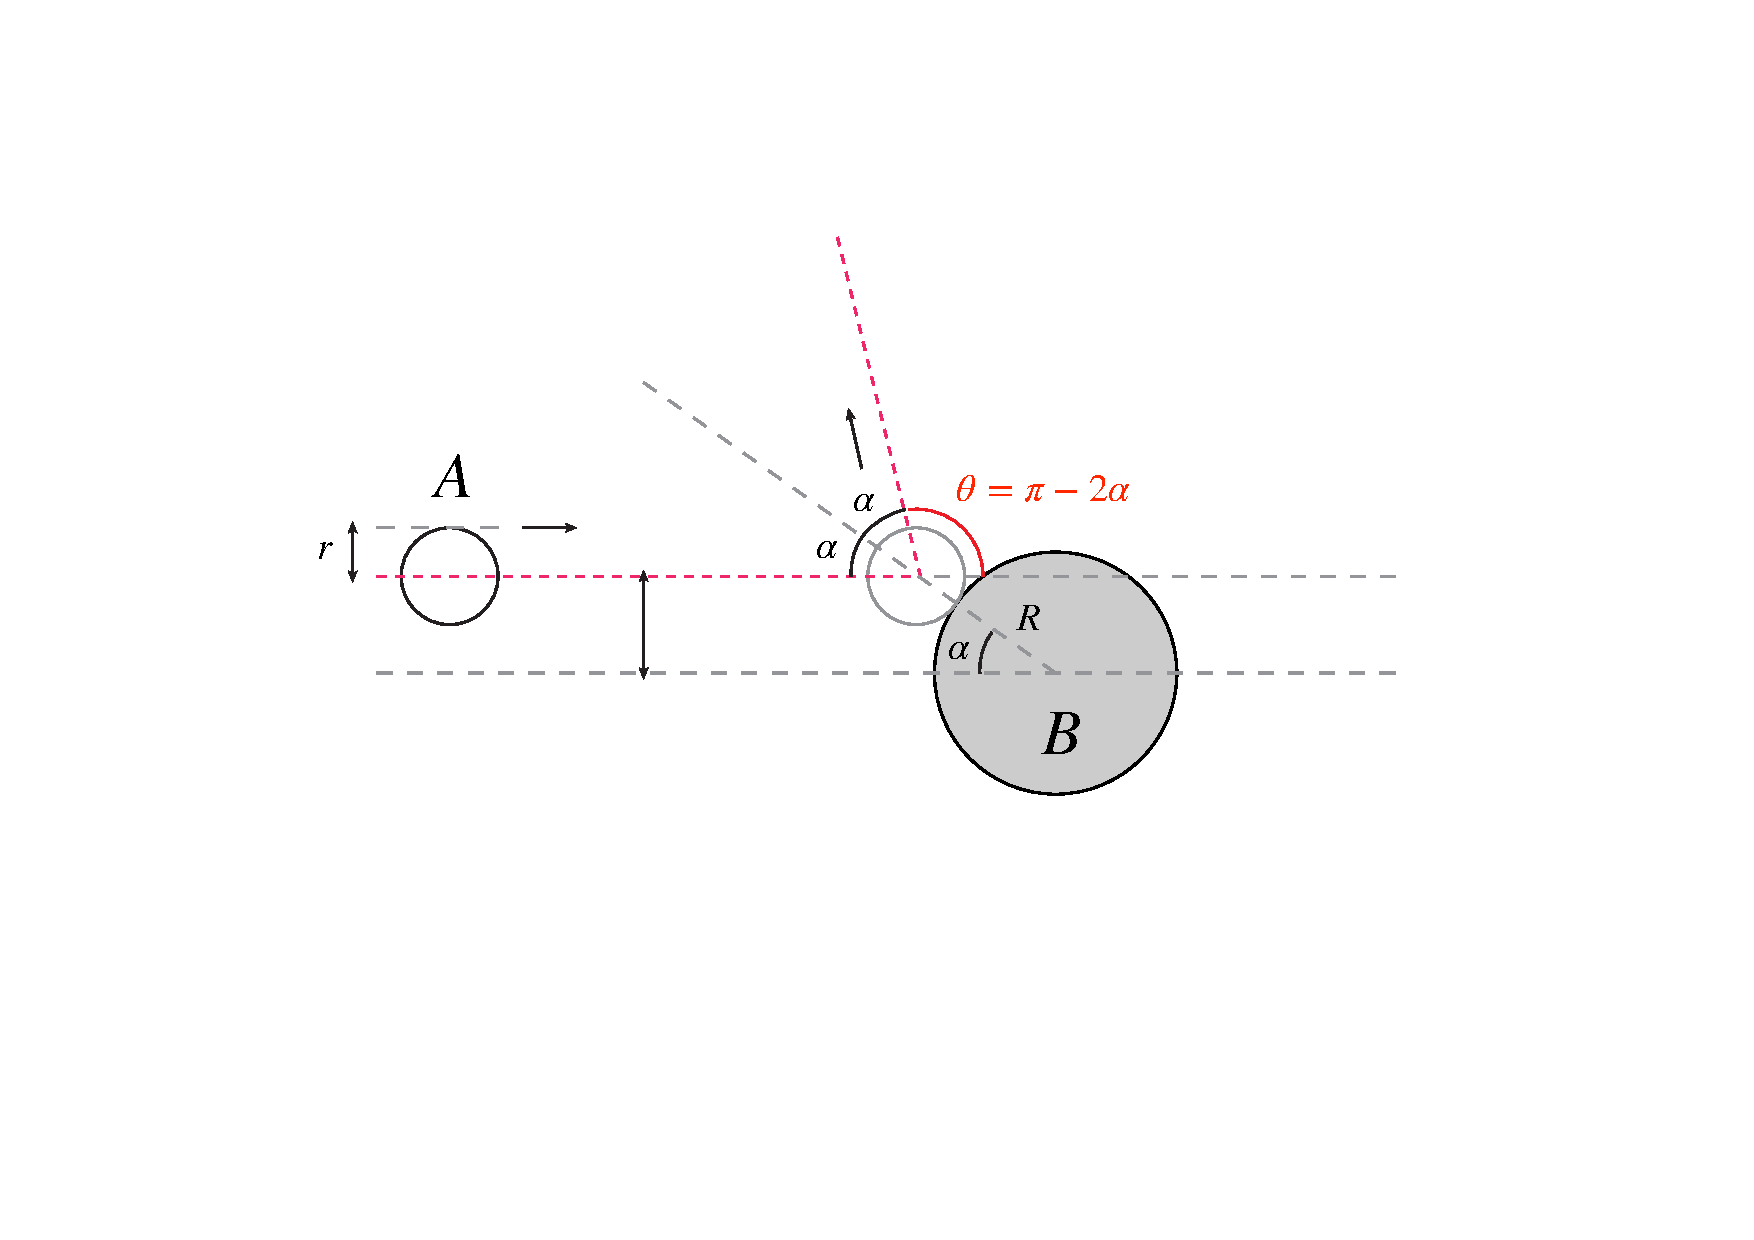
\includegraphics[width=1.0\textwidth]{Scattering-1}
    \caption{(Left) Illustration of the collision of a probe sphere (A) on a target sphere (B), in the rest frame of the target where the probe sphere has an initial velocity {\bf v}. (Right) Illustration of the relation between impact parameter and scattering angle.}
    \label{fig:spheres}
\end{figure}{}

Now, let's suppose that the nature of the target particle $B$ is not known, while that of probes is known to be hard spheres -- similarly to what happens in particle physics experiments. If it were possible to fully control the initial conditions of the incident probe and measure the resulting scattering angle -- for instance by scanning any possible impact parameter and verifying that the corresponding scattering angle $\theta$ follows the law of Eq.~\eqref{eq:spheres} -- this would corroborate the hypothesis that also $B$ is a hard sphere, i.e. the result would be an improved understanding of the nature of the target (which is the goal of the scattering experiment!).

{\it This simple macroscopic situation is unfortunately not what typically happens in a microscopic scattering experiment in atomic, nuclear or sub-nuclear physics}, where a beam of incident probe particles are bombarding an ensemble of targets, as illustrated in Figure~\ref{fig:Scattering-2}. In this case the scattering conditions are not precisely well defined, and the beam and the target are defined by an ensemble of parameters that characterize particles that are approximately in a similar dynamic state. This means that we know that all particles of the beam have similar velocities and masses, and that all targets are considered to be at rest, but we cannot "follow" individually what happens to each of those particles.

The case of \emph{colliding beams} (which is how scattering experiments at the highest energies are conducted, for example at the Large Hadron Collider at CERN) is equivalent to the case of \emph{fixed-target experiments}, as in the rest frame of one beam the collisions can be considered on fixed target. ``Colliders'' and colliding beams will be discussed briefly in Section~\ref{sec:colliders}.

The essential difference with a perfectly known beam of probe particles is that the impact parameter for each specific collision is not known. This impossibility, or in other words the non-perfectly-measurable nature of scattering experiments, has two possible fundamental origins which are completely different in nature:
\begin{itemize}
    \item Classical impossibility: a practical or experimental impossibility to measure the motion of all single particles and their trajectories.
    \item Quantum mechanics: at quantum scales, from the uncertainty principle, it is inherently impossible to  know with arbitrary precision the quantum observables which are canonic conjugates (like momentum and position, or energy and time).  
\end{itemize}

In this context, where the individual collision cannot be measured (i.e. where the individual impact parameter is not known), other observables are required to describe the dynamics of collisions.


\section{Main Definitions and notion of cross section}

Let's consider a case of a beam of particles of type $A$ colliding on a target made of particles of type $B$. We choose the reference frame in which the $B$ particles  are at rest and the $A$ particles  are traveling towards the target with a velocity $\vec{v_A}$. The transverse size of the beam of  $A$ particles is characterized by the surface ${S}$. This picture describes the laboratory frame view of a typical {\it fixed target} experiment. As mentioned in the previous section, the case of {\it colliding beams} -- where a beam of $B$ particles are traveling with a velocity $\vec{v_B}$ towards $A$ -- is fully equivalent, and just requires a change of reference frame to yield the same picture, by transforming any vector $\vec{u}$ as 
\(\vec{u} \rightarrow \vec{u} -\vec{v_B}.\)
Therefore $\vec{v_A}' = \vec{v_A}-\vec{v_B}$ and  $\vec{v_B}' = \vec{0}$. For head-on collisions, i.e. collisions where angle between the two colliding beams is zero, one simply has $v_A' = v_A+v_B$. 

We therefore assume in the following the {\it fixed target} picture, and consider a scattering experiment as illustrated in Fig.~\ref{fig:Scattering-2}, where a cylindrical beam of particles of type $A$ and surface $S$ travels with velocity $\vec{v}_A$ towards a target whose length along the beam direction is $d$, and whose transverse size is sufficient to fully contain the incoming beam.
To characterize the initial conditions of the experiment, let's first define two important quantities for modeling the scattering process.

\begin{figure}
%    \centering
    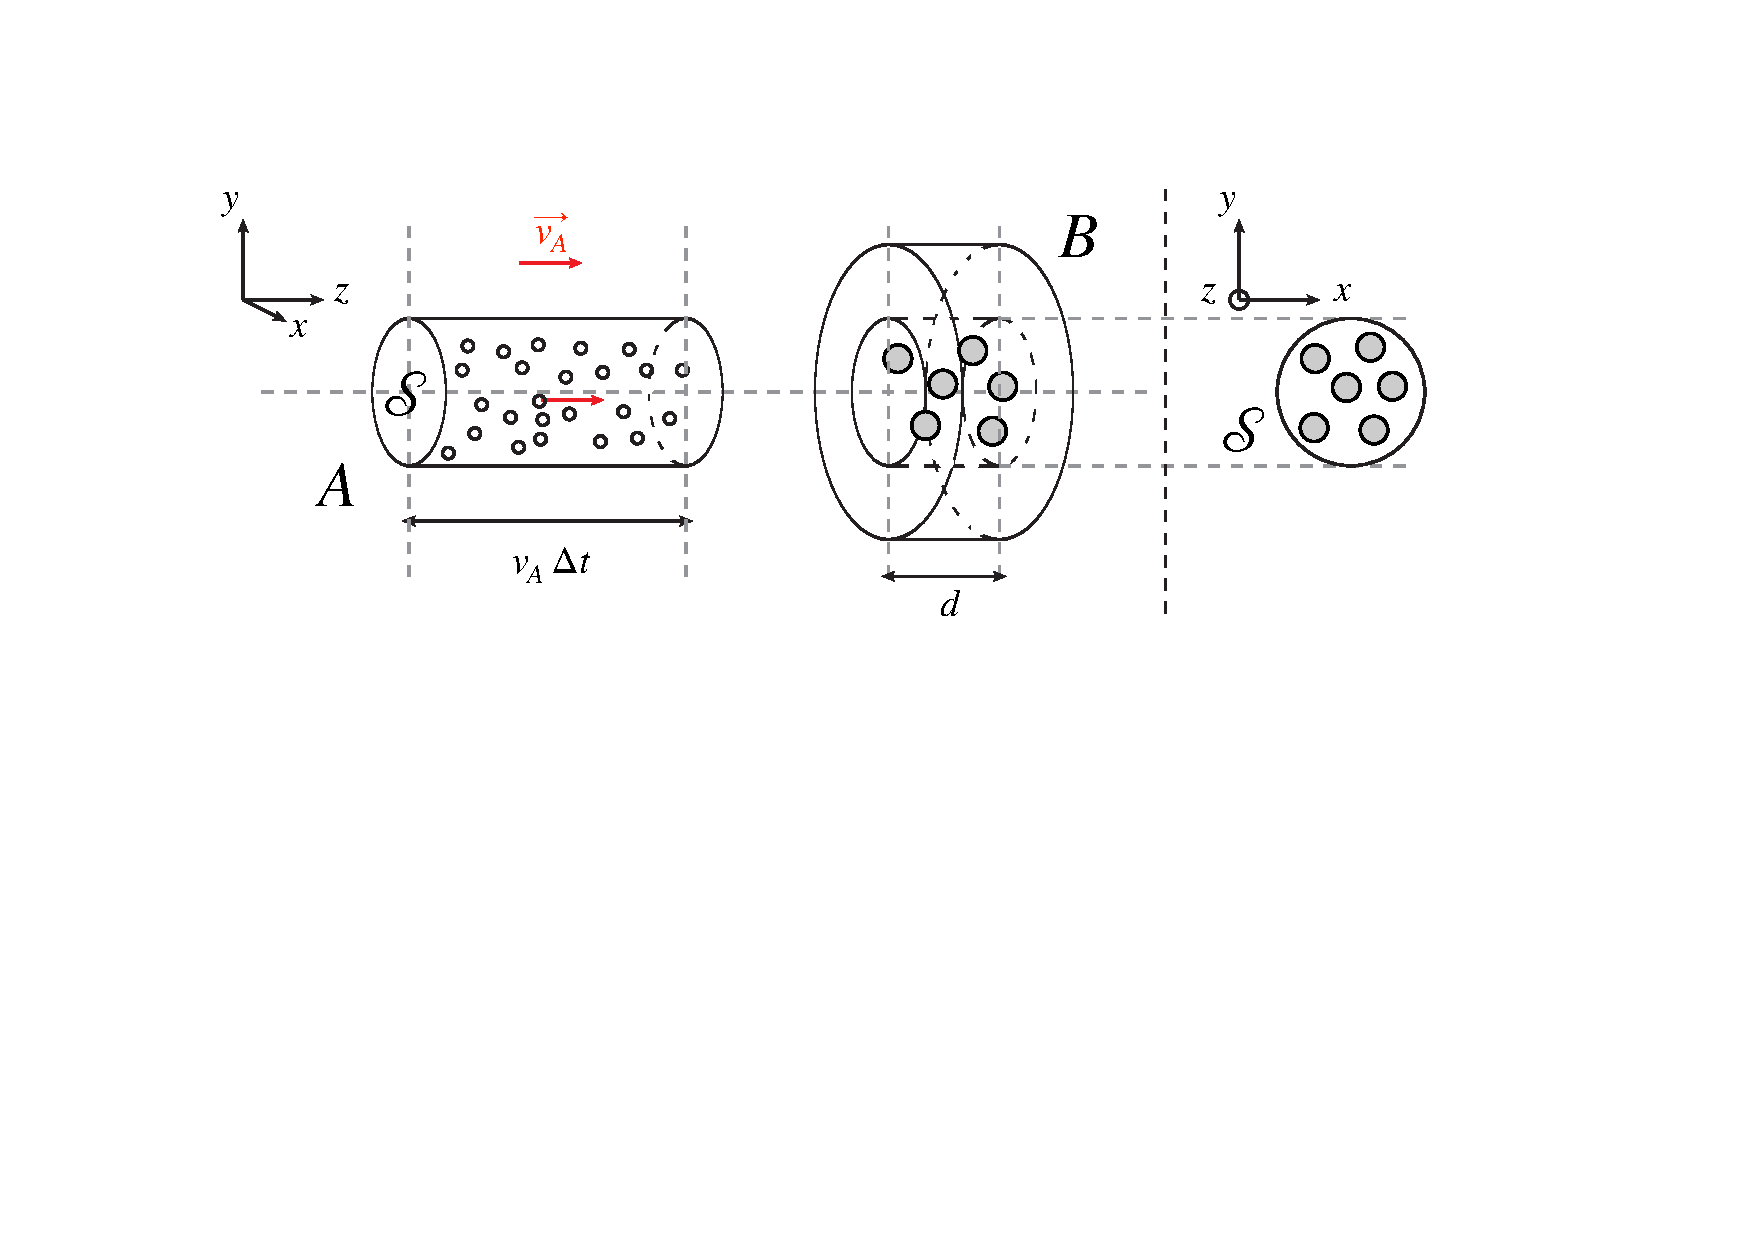
\includegraphics[width=1.0\textwidth]{Scattering-2}
    \caption{Illustration of a scattering process between a beam of surface $S$, made of particles of type $A$ and velocity $\vec{v}_A$, and a target made of particles of type $B$. The length of the target along the beam direction is $d$, and its transverse size is sufficient to fully contain the incoming beam. Left: three-dimensional view; right: view on the plane transverse to the beam direction (usually referred to as ``transverse plane'').}
    \label{fig:Scattering-2}
\end{figure}{}

\definition{{\bf The flux of beam particles $\phi_A$}: The number of particles of a beam $A$ that traverse a plane perpendicular to their motion, per unit surface and unit of time.}

The flux $\phi_A$ can be expressed in formulas as
\begin{equation*}
\begin{split}
\phi_A & =  \frac{\Delta N_A}{\Delta t} \times \frac{1}{S} \\
& =  \frac{\Delta N_A}{\Delta t \times S \times v_A} \times v_A,
\end{split}
\end{equation*}
where $\Delta N_A$ is the number of particles $A$ in the volume $S v_A \Delta t$. If we introduce the density of particles $A$ of the beam, $n_A$, we have

$$ \boxed{\phi_A = n_A \times v_A. }$$

The other important definition, in this {\it fixed target} view, is the number of targets that are ``seen'' by the beam, which can also be expressed in terms of the density of  $B$ particles, $n_B$, as

\[ \boxed{N_B = n_B \times S \times d.}\]

$N_B$ and $\phi_A$ characterise the initial conditions of the scattering experiment. 


Now, in order to gather information about the nature of the interacting particles or about the interaction itself, the result of the scattering experiment is simply expressed as a number of counts per unit time, i.e. a {\bf rate}. This concept will be further developed in the next section; in order to get there, we first need to introduce a concept which is best understood with the simple geometrical example of colliding spheres: the concept of {\bf scattering cross section}.

What we are looking for is the best way to quantitatively describe the interaction between two particles $A$ and $B$ from the main observable of a scattering experiment, the scattering rate $\od{N_I}{t}$.

For the simple example of scattering sphere, let's first estimate the number of interactions of a particle $A$ during a short time interval $\Delta t$. Considering that the particle $A$ is taken at random {\it uniformly} in the beam volume $S \times v_A \times \Delta t$, the number of targets that the particle $A$ will ``see'' during this time will simply be $n_B \times S \times v_A \Delta t$.

\begin{figure}
    \centering
    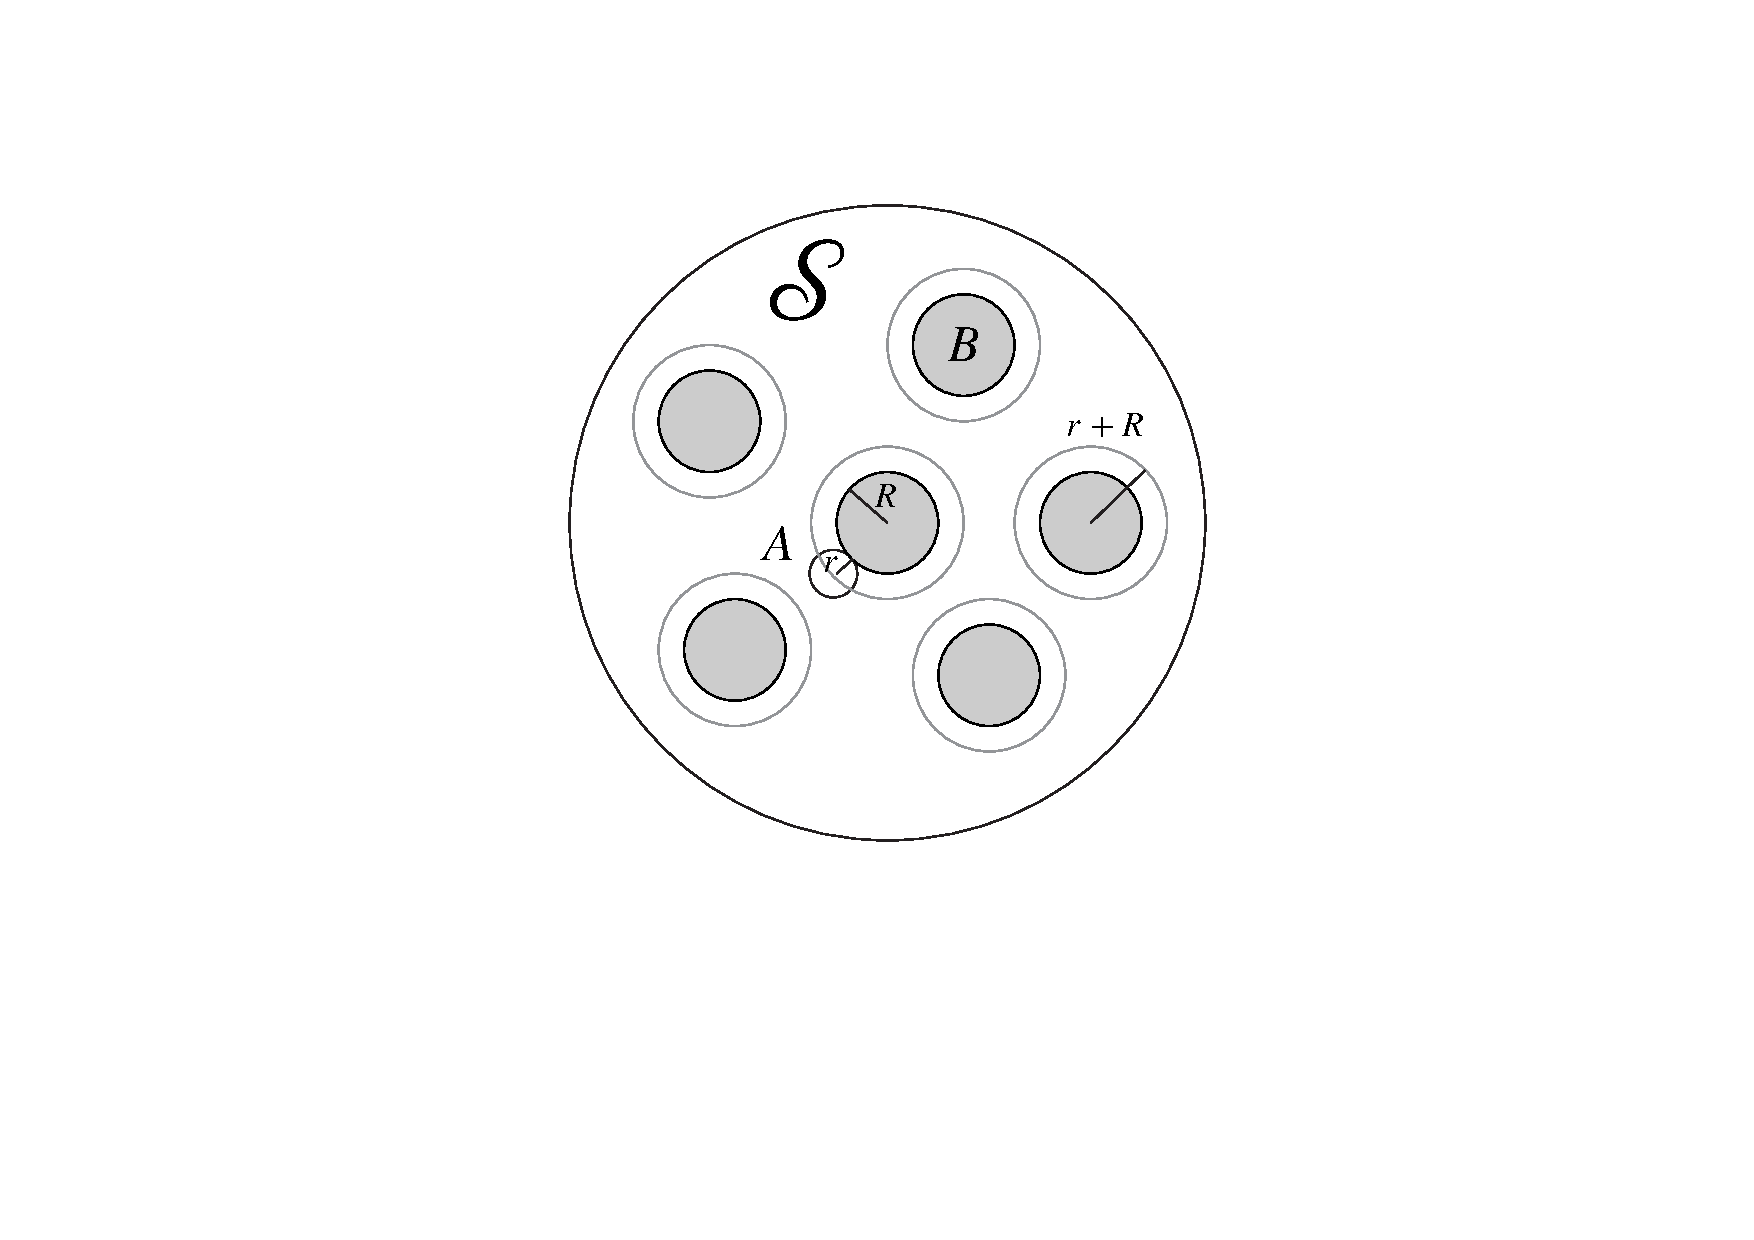
\includegraphics[width=0.4\textwidth]{Scattering-3}
    \caption{Illustration of the available scattering surface within the surface area of the beam. This transverse view corresponds to a slice of width $v_A \Delta t$.}
    \label{fig:Scattering-3}
\end{figure}{}

Let us compute, for each particle $B$, the probability for $A$ and $B$ to interact, by considering the distribution of $A$ and $B$ to be uniform over the slice of the beam, and considering that a contact between the spheres will occur if the impact parameter $b$ will be smaller than $r+R$. The probability $\delta P$ of the two to be in contact will simply be the ratio between the ``contact'' surface and the entire surface of the beam, i.e.

\[ \delta P = \frac{\pi (r+R)^2}{S} \equiv \frac{\sigma}{S}, \]

\noindent where $\sigma = \pi (r+R)^2$. For a given $A$ particl to interact with \emph{any}  $B$ particle within the slice of beam considered, the probability of an interaction $\Delta P$ will then be

\[ \Delta P = \delta P \times n_B v_A S \Delta t.\]

The next step is to extend the calculation to the beam traversing the entire width of the target $d$ -- which requires that the beam length is longer than the target. The total number of $A$ particles that can interact is then $n_A \times S \times d$.

The number of interactions per unit time for a beam crossing the target will thus be

\[\frac{\Delta N_I}{\Delta t} =\frac{\Delta P}{\Delta t} \times N_A= \frac{\Delta P}{\Delta t} \times n_A \times S \times d. \]

The {\bf rate} of interactions will therefore be:

\begin{align*}
\frac{\Delta N_I}{\Delta t} & =  n_A \times S \times d \times n_B \times v_A \times \sigma \\
& =  (n_A v_A) \times (n_B \times S \times d) \times \sigma.
\end{align*}

This simple equation describes how the rate of events can be expressed in terms of the initial conditions of the beam and the target and the cross section which describes the probability of an interaction between a particle $A$ and a particle $B$ as a fraction of the surface area of the beam.


\definition{{\bf The scattering cross section} is defined for any scattering process by generalising the geometrical description of the example above: the cross section is the quantity  $\sigma$ which allows to express the rate of a scattering process as

$$ \boxed{ \frac{\Delta N_I}{\Delta t}  =  \phi_A \times N_B \times \sigma}.$$

}

Cross section has the units of a surface.
In the processes relevant for nuclear and subnuclear physics, cross sections are typically of the order of magnitude of the size of nuclei -- for instance as $^{238}U$, which was deemed to be {\it "as big as a barn"}. This defines the typical unit of cross section, i.e. $10^{-28}$~m$^2$:

$$\boxed{1 \; {\rm barn} = 1 \; {\rm b} = 10^{-28} \; {\rm m^2} }.$$

Another important definition which further simplifies the equation defining the cross section is that of luminosity.

\definition{{\bf Luminosity}: the luminosity $\mathcal{L}$ determines the initial conditions of the scattering experiment, and is defined as
$$\boxed{\mathcal{L} = \phi_A \times N_B }.$$

Luminosity is often expressed in units of $[\mathcal{L}]=\si{cm^{-2}s^{-1}}$.
}

\section{Differential Cross Section}\label{sec:sfererigide}

In order to be able to fully characterise the interaction, it is important to measure all measurable properties of the scattered particles (i.e. reconstruct the final state of the interaction fully). When the nature of the particle is known, the measurable quantities for a scattering experiment are its direction and energy in the final state (assuming that knowing its nature means knowing its mass and therefore its momentum is fixed). Typically the cross section is then measured in a differential fashion, by counting the number of particles per unit time (i.e. the rate) as a function of the particle's energy and direction in spherical coordinates $(E,\theta, \phi)$. 

A typical scattering experiment is illustrated in Fig.~\ref{fig:Scattering-4}, where a detector measuring a small portion of solid angle $d\Omega$ is considered.

\begin{figure}
%    \centering
    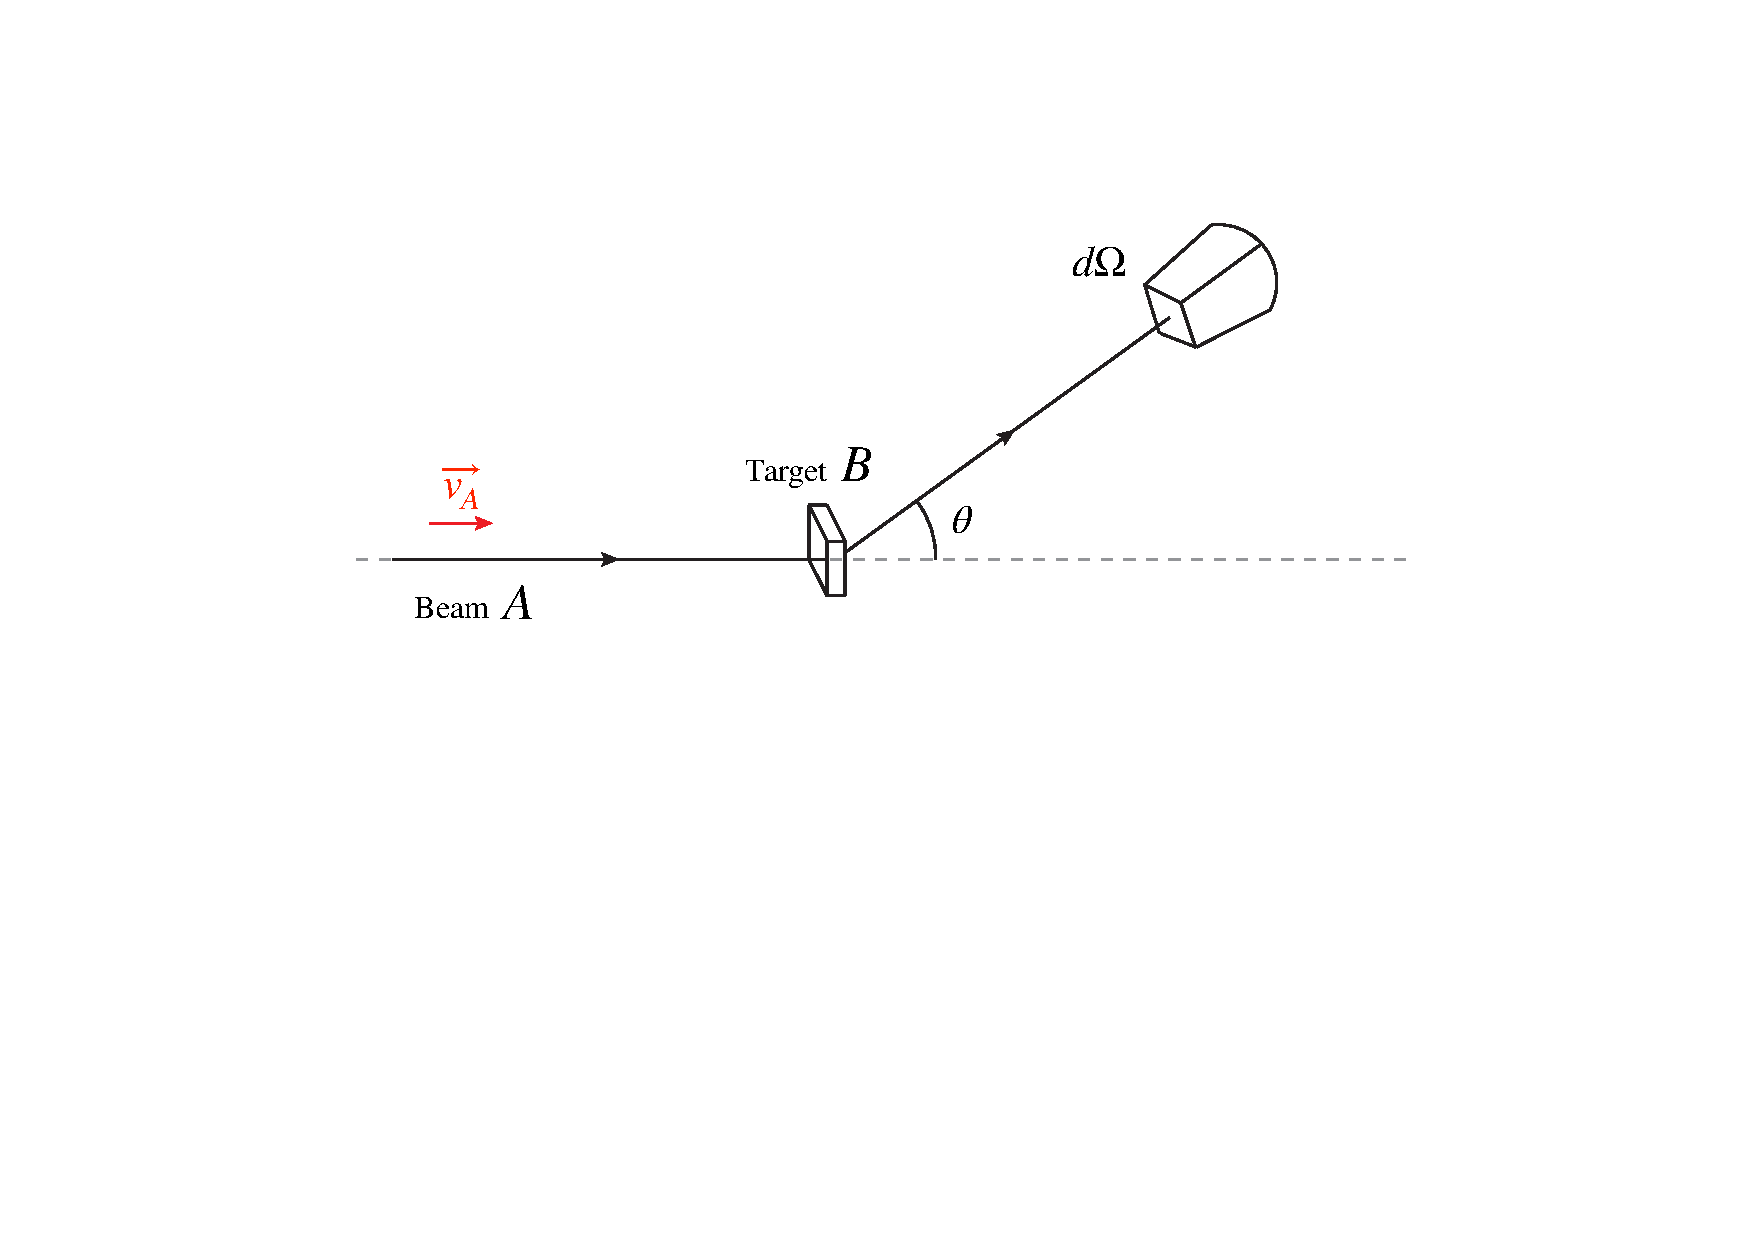
\includegraphics[width=0.9\textwidth]{Scattering-4}
    \caption{Illustration of a typical scattering experiment measuring a differential cross section $\sigma(E, \theta, \phi)$ of the scattering of particles of type $A$ on a target of particles $B$.}
    \label{fig:Scattering-4}
\end{figure}{}

The differential cross section will then be defined again with respect to the rate of specific scatterings in the $(E,\theta, \phi)$ phase space, yielding

\[
\frac{\Delta N_I}{\Delta t} (E,\theta, \phi) = \dot{N}_I (E,\theta, \phi) = \phi_A N_B \sigma (E,\theta, \phi).
\]

Given that the differentiation comes from the phase space in the final state, the only dependence that relates the initial state to the final state being the cross section (as $\mathcal{L}$ is a constant), one can then write
\[\frac{d^3\sigma}{dE d\theta d\phi}(E,\theta,\phi) = \frac{d^3 \dot{N}_I 
(E,\theta,\phi)}{dE d\theta d\phi} \times \frac{1}{\mathcal{L}}.\]
Or, in other typical cases where there is a cylindrical symmetry (uniform scattering in the azimuthal angle $\phi$) and a scattering where the final state energy of the measured particle is fixed, then the relevant quantity will be
\[\frac{d\sigma}{d\Omega}(\theta) = \frac{d \dot{N}_I}{
d\Omega}(\theta) \times \frac{1}{\mathcal{L}}.\]
From this differential cross section, the interaction rate at a certain scattering angle $\theta$ within a solid angle $d\Omega$ can be derived. In all of these cases, we are always doing the same thing: expressing the probability of the interaction in terms of quantities which define the ``parameter space'' in which we measure the scattering (i.e. the interaction rate). Choosing with respect to which variables we express the differential cross section is a matter of knowing how the scattering experiment is conducted -- whether our particle detectors cover the full solid angle or not, whether we measure energies or angles or we can assume some symmetry of the system, etc.

We can then return to the simple case of colliding spheres and compute the prediction of the differential cross section.

As we have seen in this case, the energy or velocity of the scattered sphere is constant and equal in norm to the initial velocity $v_A$. The scattered spheres will be uniformly distributed in the azimuth direction $\phi$ -- there is no reason for them to prefer any specific value of $\phi$. We can then compute the differential cross section as a function of the polar scattering angle $\theta$, which will correspond to a specific element of solid angle $d\Omega$ that can be integrated over $\phi$. We have seen that  a given scattering angle $\theta$ corresponds to a specific value of the {\it impact parameter} $b$. The scattered particles $A$ will be in the element solid angle $d\Omega$ if the impact parameter $b$ lies in the interval $[b, b+db]$. If we look at the collision in the transverse plane with respect to the beam direction (Fig.~\ref{fig:Scattering-5}), this allows to estimate the probability of an interaction in these conditions, which corresponds to the ratio between the area of the ring and the total surface, $2\pi b db/S$. Following the same reasoning as for the total cross section, one can write the contribution to the total rate corresponding to this ``ring'' as
\[
d \dot{N}_I = d \sigma (b) \times \phi_A \times N_B,
\]
where according to Fig.~\ref{fig:Scattering-5} one has
\[d\sigma (b) = 2 \pi b db.\]

\begin{figure}
    \centering
    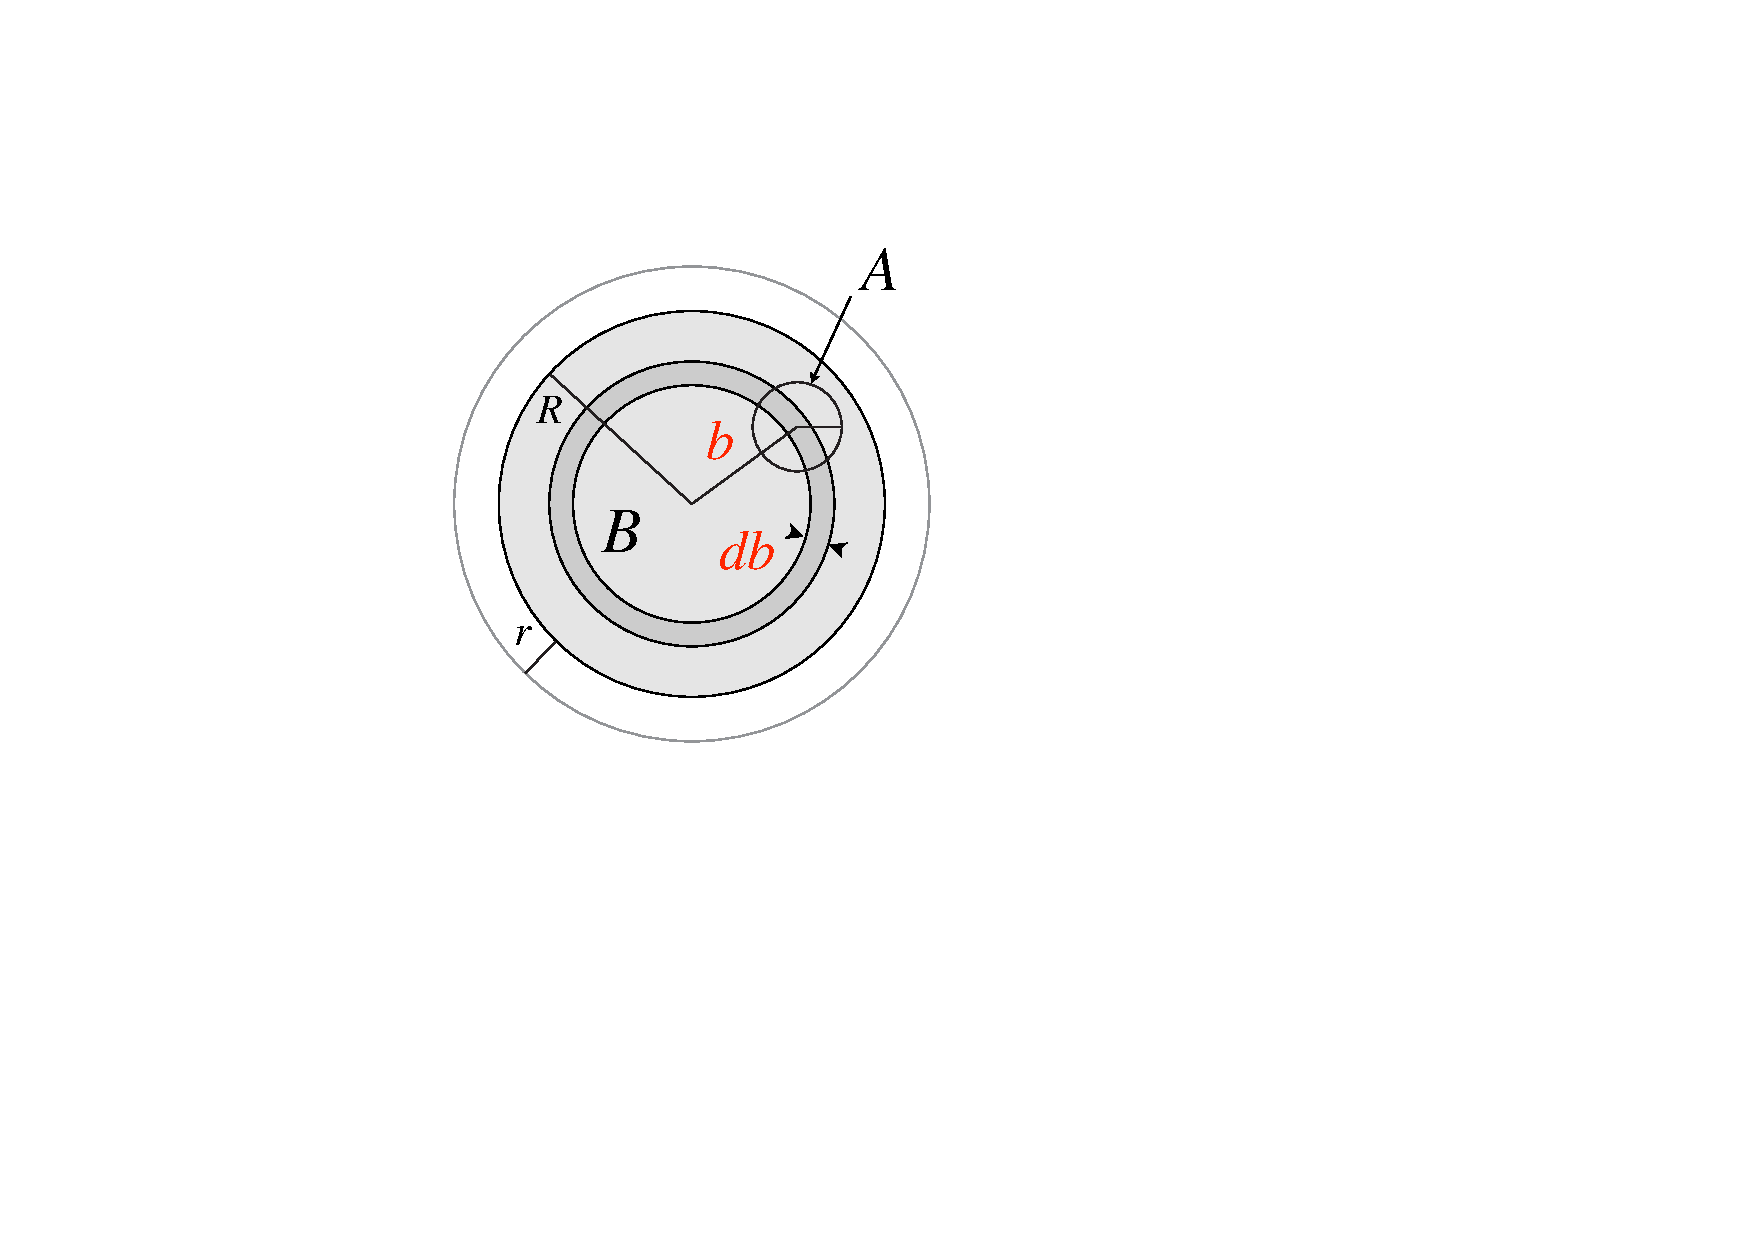
\includegraphics[width=0.5\textwidth]{Scattering-5}
    \caption{Illustration (in the shaded area) of the surface area representing the cross section for a scattering corresponding to an impact parameter $b$ and its corresponding scattering angle.}
    \label{fig:Scattering-5}
\end{figure}{}

Then the differential rate can be written from the relation between the impact parameter and the scattering angle $b=(R+r) \cos \frac{\theta}{2}$:

\begin{align*}
    d \dot{N}_I & = 2 \pi (R+r) \cos \frac{\theta}{2} \times \mathcal{L} \times db \\
    &= 2 \pi (R+r) \cos \frac{\theta}{2} \times \mathcal{L} \times \left | \frac{db}{d\theta} \right  | d\theta \\
    &= 2\pi (R+r)^2 \frac{1}{2} \cos \frac{\theta}{2} \sin \frac{\theta}{2} \times \mathcal{L} \times d\theta \\
    &= 2 \pi \sin \theta \times \frac{(R+r)^2}{4} d\theta \times \mathcal{L}.
\end{align*}
Here used the relation between the impact parameter and scattering angle, from which one has
\[\od{b}{\theta} = \frac{R+r}{2}\od{ \cos \frac{\theta}{2}}{\theta} = - \frac{R+r}{2} \sin \frac{\theta}{2}.\]

Now, let us consider an element solid angle in spherical coordinates $d\Omega = \sin \theta d\theta d\phi$. Since scattering is uniform in the azimuthal angle $\phi$, the element solid angle can be expressed as

\[ d\Omega = \sin \theta d\theta \int_0^{2\pi} d\phi = 2\pi \sin \theta d\theta,\]
and the differential rate can be written as
\[\od{\dot{N}_I}{\Omega} = \frac{(R+r)^2}{4} \times \mathcal{L},\]
so that the differential cross section is
\[\frac{d \sigma}{d \Omega} = \frac{(R+r)^2}{4}.\]
This implies that the distribution of the scattering of two spheres is uniform in any direction! The rate measured by a detector will be the same in any direction. 

We can then see for consistency what happens when the differential cross section is integrated over the entire solid angle:
\[ \sigma = \int_0^{4\pi} \left ( \frac{d\sigma}{d\Omega} \right ) d\Omega = \pi (r+R)^2,\]
which is precisely the initial result for the total cross section $\sigma$.

The reasoning we followed here in the simple, ideal example of colliding hard spheres is the same which is used in any scattering experiment. The task will be to determine which quantities are measured in the final state, and to calculate the differential and total cross-section of the interaction -- which is in general a measurement of its probability, rather than of the ``physical size'' of the involved particles.

\section{Absorption Coefficient and Mean Free Path}

In this section the important notions of absorption coefficient and mean free path will be introduced. These two concepts will prove essential for describing quantitatively what happens when particles travel through matter. %These notions will be very important in Chapter~\ref{}. 

\subsection{Absorption coefficient}
Let us consider a beam of particles $A$ on a target of particles $B$. The probability for a given particle of a beam to interact on a element distance $dx$ will be constant,
\[dP = \sigma n_B dx,\]
where $n_B$ is the density of particles $B$. We can then define the quantity
\[\mu = \sigma n_B,\]
so that the variation in the flux of the beam on a length $dx$ can be written as
\[d\phi = -\phi dP = -\phi \mu dx,\]
therefore
\[ \frac{d\phi}{\phi} = -\mu dx \; \; {\rm i.e.} \; \; [log \phi]_{\phi_0}^{\phi} = -\mu x,\]
or 
\[\boxed{\phi(x) = \phi_0 e^{-\mu x}.}\]
The dimensions of $\mu$ will then be those of the inverse of a length, as $[\mu]=[\sigma][n_B] = \si{m^2} \times \si{m^{-3}} = \si{m^{-1}}$. 

\definition {\textbf{The absorption coefficient} is defined as the product between the cross section and the number of targets per unit volume,

\[ \mu = \sigma n_B.\]

The \textbf{attenuation length} $\lambda$ is defined as its reciprocal, i.e.

\[ \lambda = \frac{1}{\mu}.\]}

The attenuation length corresponds to the length after which the flux of incoming particles gets reduced by a factor $e$ (i.e. where $\phi(x=\lambda) = \phi_0 / e$).

\subsection{Mean free path}
The mean free path is the average distance covered by a particle in a target between two successive interactions. Let us then first consider a distance $x$ along the path of the particle from a point $O$ with coordinate $0$ in the $x$ direction. The distance $x$ represents the distance between two interactions (or ``scatterings''), one occurring at $0$ and the subsequent occurring at $x$.

In order to compute the probability of having a distance $x$ between two scatterings, one has to follow two steps. 
First the probability for the probe particle {\it not to have interacted} between $0$ and $x$ ($P_{NI}(x)$) can be computed from integrating its differential form
\[ dP_{NI}(x) = P_{NI}(x+dx) - P_{NI}(x), \; \; {\rm where} \; \; P_{NI}(x+dx) = P_{NI}(x) (1 -\mu dx),\]
which means that the probability of not having interacted in $x+dx$ can simply be deducted from the probability of not having interacted in $x$. Then, one has
\[dP_{NI}(x) = -\mu \, dx \, P_{NI}(x) \; \; \Longrightarrow \; \; \left[\ln P_{NI}\right]_{0}^{x} = \mu \, x.\]

Assuming that $P_{NI}(0) = 1$, the probability of {\it not having interacted} in $x$ will then be
\[P_{NI}(x) = e^{-\mu \, x}.\]
The probability of interacting after $x$ (but not before!) will then be
\[P(x)\, dx = P_{NI}(x) \times \mu \, dx = \mu e^{-\mu \, x}\, dx.\]
If we average all the possible path lengths $x$ weighted by their probability, we get the average path:
\begin{align*}
    \langle x\rangle & = \int_0^{\infty} x \cdot P(x) dx \\
    & = \int_0^{\infty} x  \mu e^{-\mu \, x}dx \\
     & = \frac{1}{\mu} \int_0^{\infty}  (\mu \, x) e^{-\mu \, x} d(\mu \,x) \\
     &= [-e^y (1+y)]_0^{\infty} \; \; \qquad (y=\mu \, x) \\
     &= \frac{1}{\mu},
\end{align*}
where the integration is simply done by parts.

\definition{{\bf The mean free path} of a particle is the average length traveled by a particle between two subsequent interactions,
\[\langle x\rangle = \lambda.\]
}
One can immediately see that the mean free path is equivalent to the attenuation length, as defined in the previous section.

\section{The Rutherford Scattering Experiment} 

These definitions can be immediately applied to the analysis of one of the most fundamental, landmark experiments for our understanding of atoms: the Rutherford experiment. 

\subsection{Early atomic model} 

Towards the turn of the XX century, it was understood that the atom was made of positive charges and electrons. Thomson then proposed the idea of a dynamic model where the electrons -- which were understood to be particles after his own experiment -- would be embedded in a volume filled with a positively charges. Thomson considered three hypotheses on how the electrons could be distributed with respect to the positive charges. The first was that the electrons were embedded in a uniformly positively-charged medium, the second was to pair each electron with a positive charge and the third was that the negatively-charged particles would orbit inside a volume of positive charges. Thomson retained the first hypothesis as the most likely. This model is often referred to as the ``plum pudding'' model, where the electrons are modelled as ``plums'' evenly distributed within a ``pudding'' or positively-charged continuum (see an illustration of the ``plum pudding"model'' on the left of Fig.~\ref{fig:RutherfordAtom}).

\begin{figure}
    \centering
    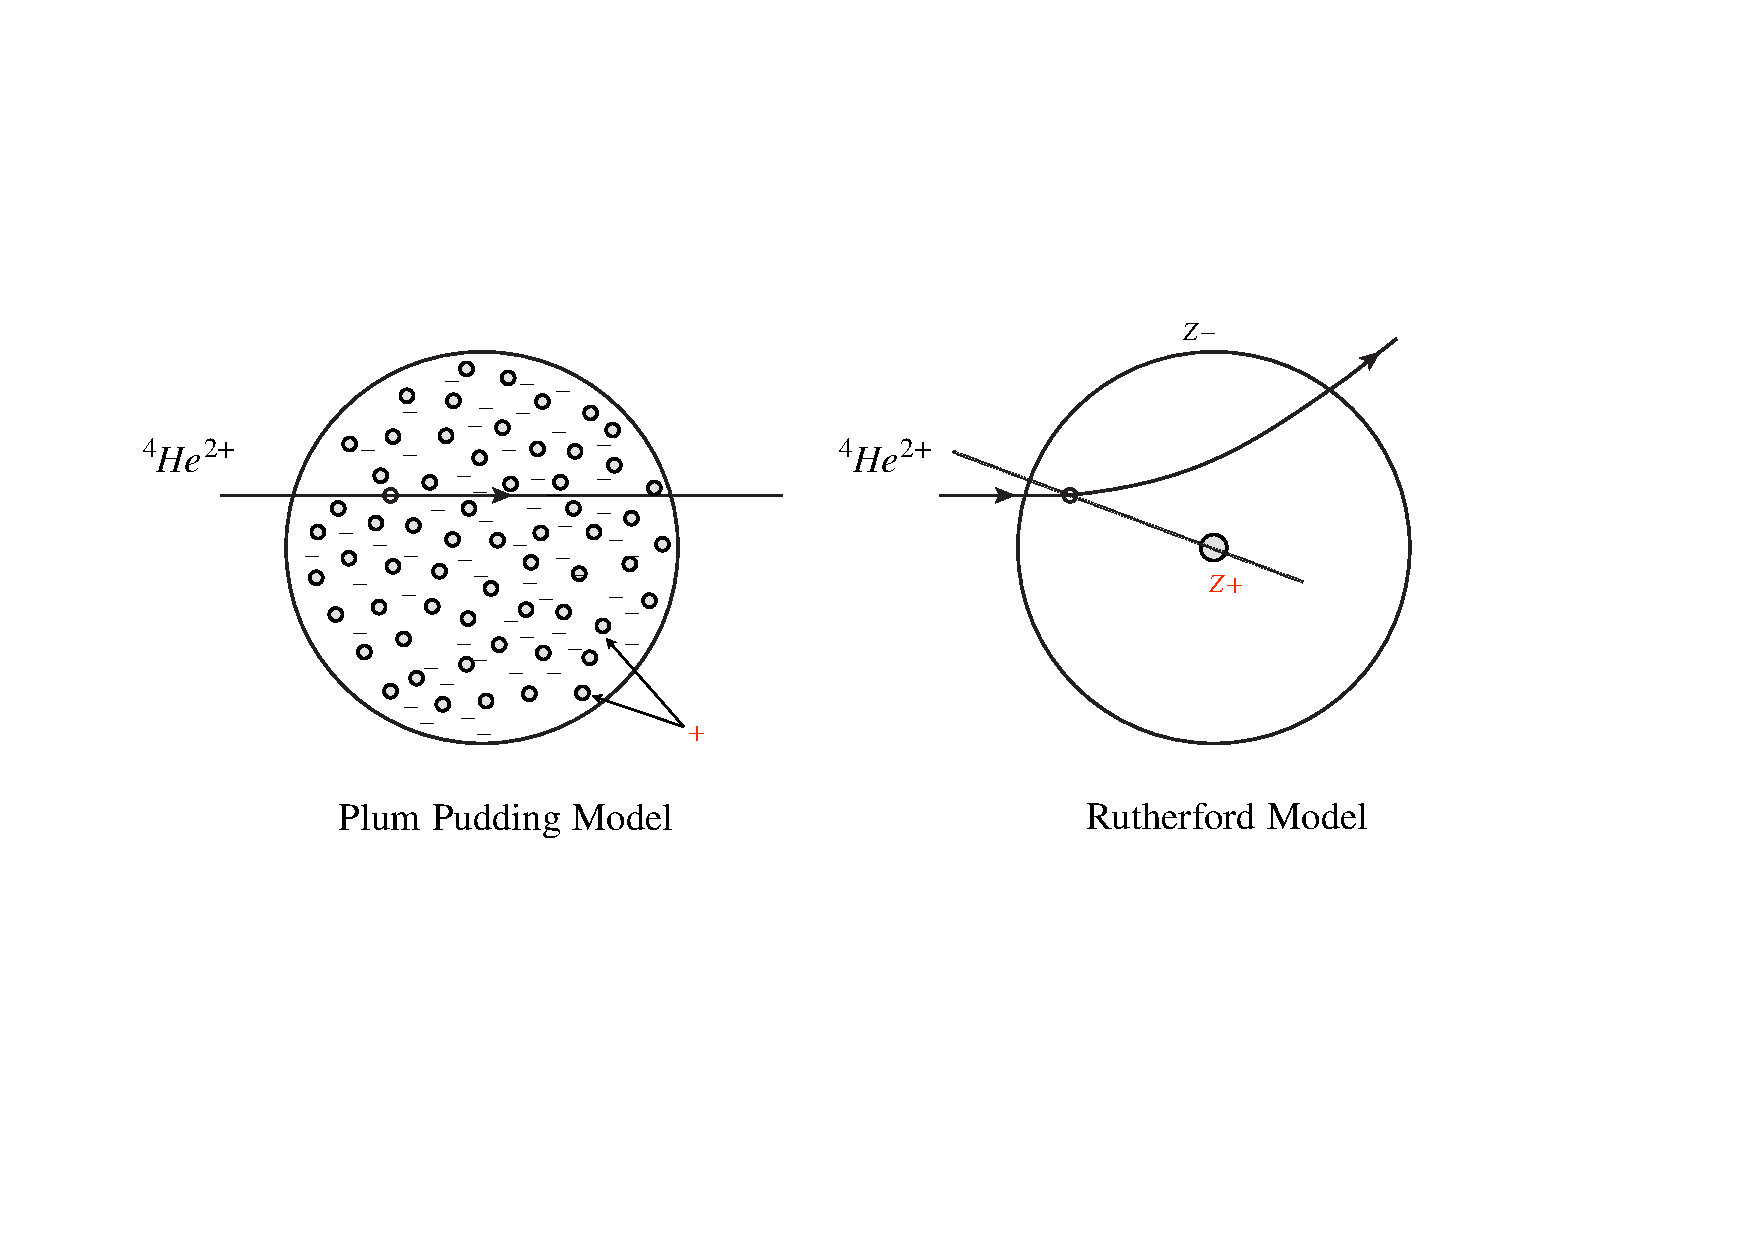
\includegraphics[width=0.9\textwidth]{Scattering-7}
    \caption{(Left) Early atomic model by Thomson and illustration of an $\alpha$ particle traversing it unperturbed. (Right) Illustration of the Rutherford model where all positive charges are concentrated in a positively-charged nucleus at the centre of the atom. The trajectory of an $\alpha$ particle is shown as well.}
    \label{fig:RutherfordAtom}
\end{figure}{}

Thomson encouraged his student at the time, Ernest Rutherford, to pursue experiments to probe models of the atom. In order to do so, they exploited the idea of using $\alpha$ particles ($^4He^{2+}$) to probe the structure of the atom, as shown in Fig.~\ref{fig:RutherfordAtom}. 

In the case of the ``plum pudding'' model (left figure), no deviation of the $\alpha$ particles is expected. This can be understood from the fact that, at any time, the electric field created by the charges in the atom can be separated into two contributions: the first is the outer spherical and hollow shell volume at a radius with respect to the centre of the atom which is larger than the distance of the $\alpha$ particle to the atom's centre, as illustrated in Fig.~\ref{fig:gauss}-a; the second is the inner sphere as illustrated in Fig.~\ref{fig:gauss}-b.

Since the atom is neutral, when the $\alpha$ particle travels outside of the atom it will ``sense'' no electric field. When inside the atom, the contribution of the electric field on the $\alpha$ particle from the outer hollow spherical shell volume is $0$ from Gauss' theorem, as there are no charges inside the inner volume. The component from the inner sphere can be computed as well using Gauss' theorem: one has
\[ \varoiint \vec{E} \cdot d\vec{S} = 4\pi r^2 E \frac{1}{\varepsilon_0} \iiint \rho dV = \frac{Q}{\varepsilon_0} = 0,\]
i.e. the electric field generated by the inner sphere will  also be equal to $0$. In this model the $\alpha$ particle should travel through the atom mostly unperturbed!

In the case where the positive charges are concentrated in a limited volume at the centre of the atom, the situation is quite different. When inside the inner shell of electrons, the $\alpha$ particle will be fully subject to the electric field of the charges at the centre of the atom (see Fig.~\ref{fig:gauss}-b).

\begin{figure}
    \centering
    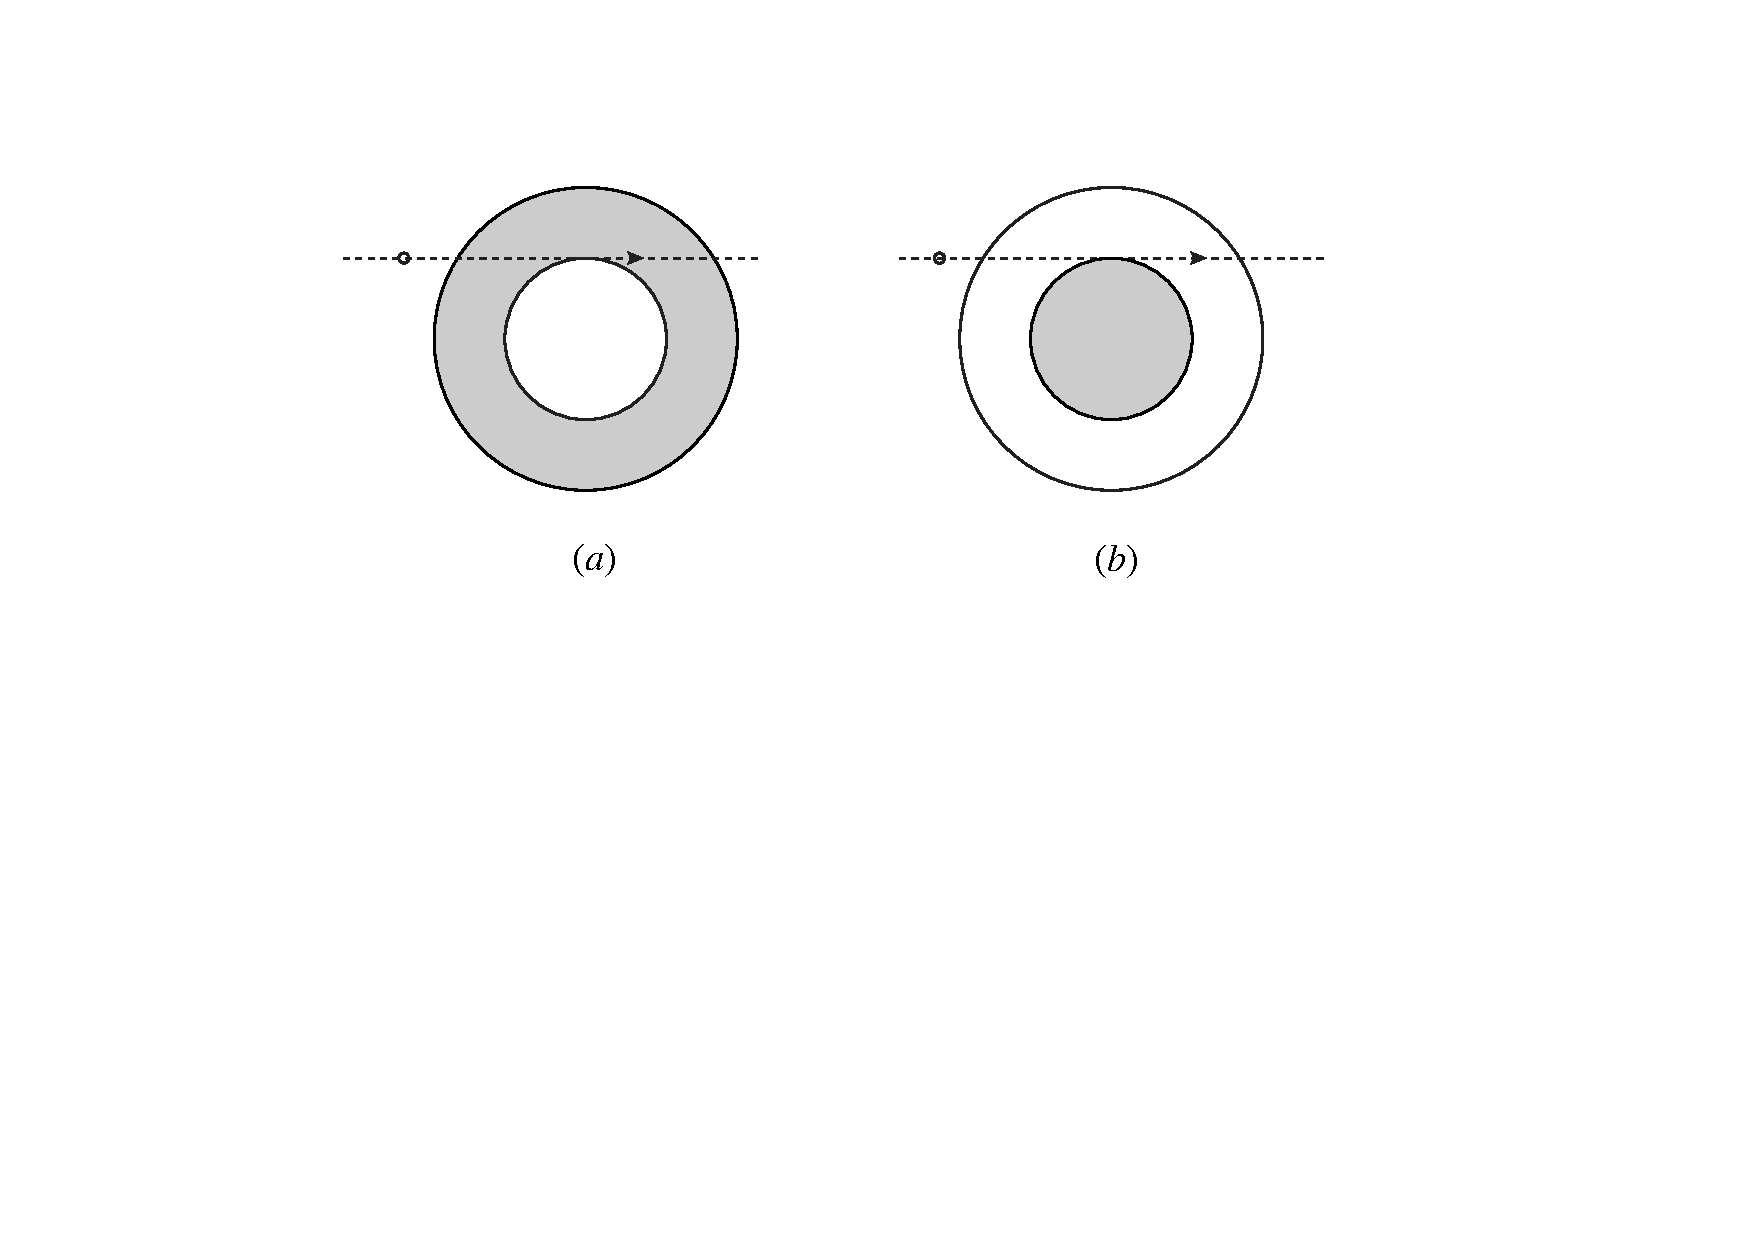
\includegraphics[width=0.9\textwidth]{Scattering-8}
    \caption{Illustration of the two volumes of charges that are considered in order to derive the trajectory of an $\alpha$ particle within an atom in the ``plum pudding'' model.}
    \label{fig:gauss}
\end{figure}{}

\subsection{The Rutherford scattering experiment}

Rutherford started his experiments with Hans Geiger in 1907, joined by Ernest Marsden in 1909 at the University of Manchester. In 1912, the team was joined by Niels Bohr to study the atom.

The setup of the Rutherford-Geiger-Marsden experiment is illustrated in Fig.~\ref{fig:geiger-marsden}. The team used a radium source to generate the beam of $\alpha$ particles, which impinged on a target made of gold foil. The system was designed to measure the scattering at large angles: for this reason, the main detection device (the microscope and the screen) could rotate around the target. The idea of the detector is that the passage of $\alpha$ particles through the screen of zinc sulfate would generate a faint scintillation light that could be visible if the eye was sufficiently accustomed to the dark (which took about half an hour during the experiment). The source generated a "beam" of collimated $\alpha$ particles. 

\begin{figure}
    \centering
    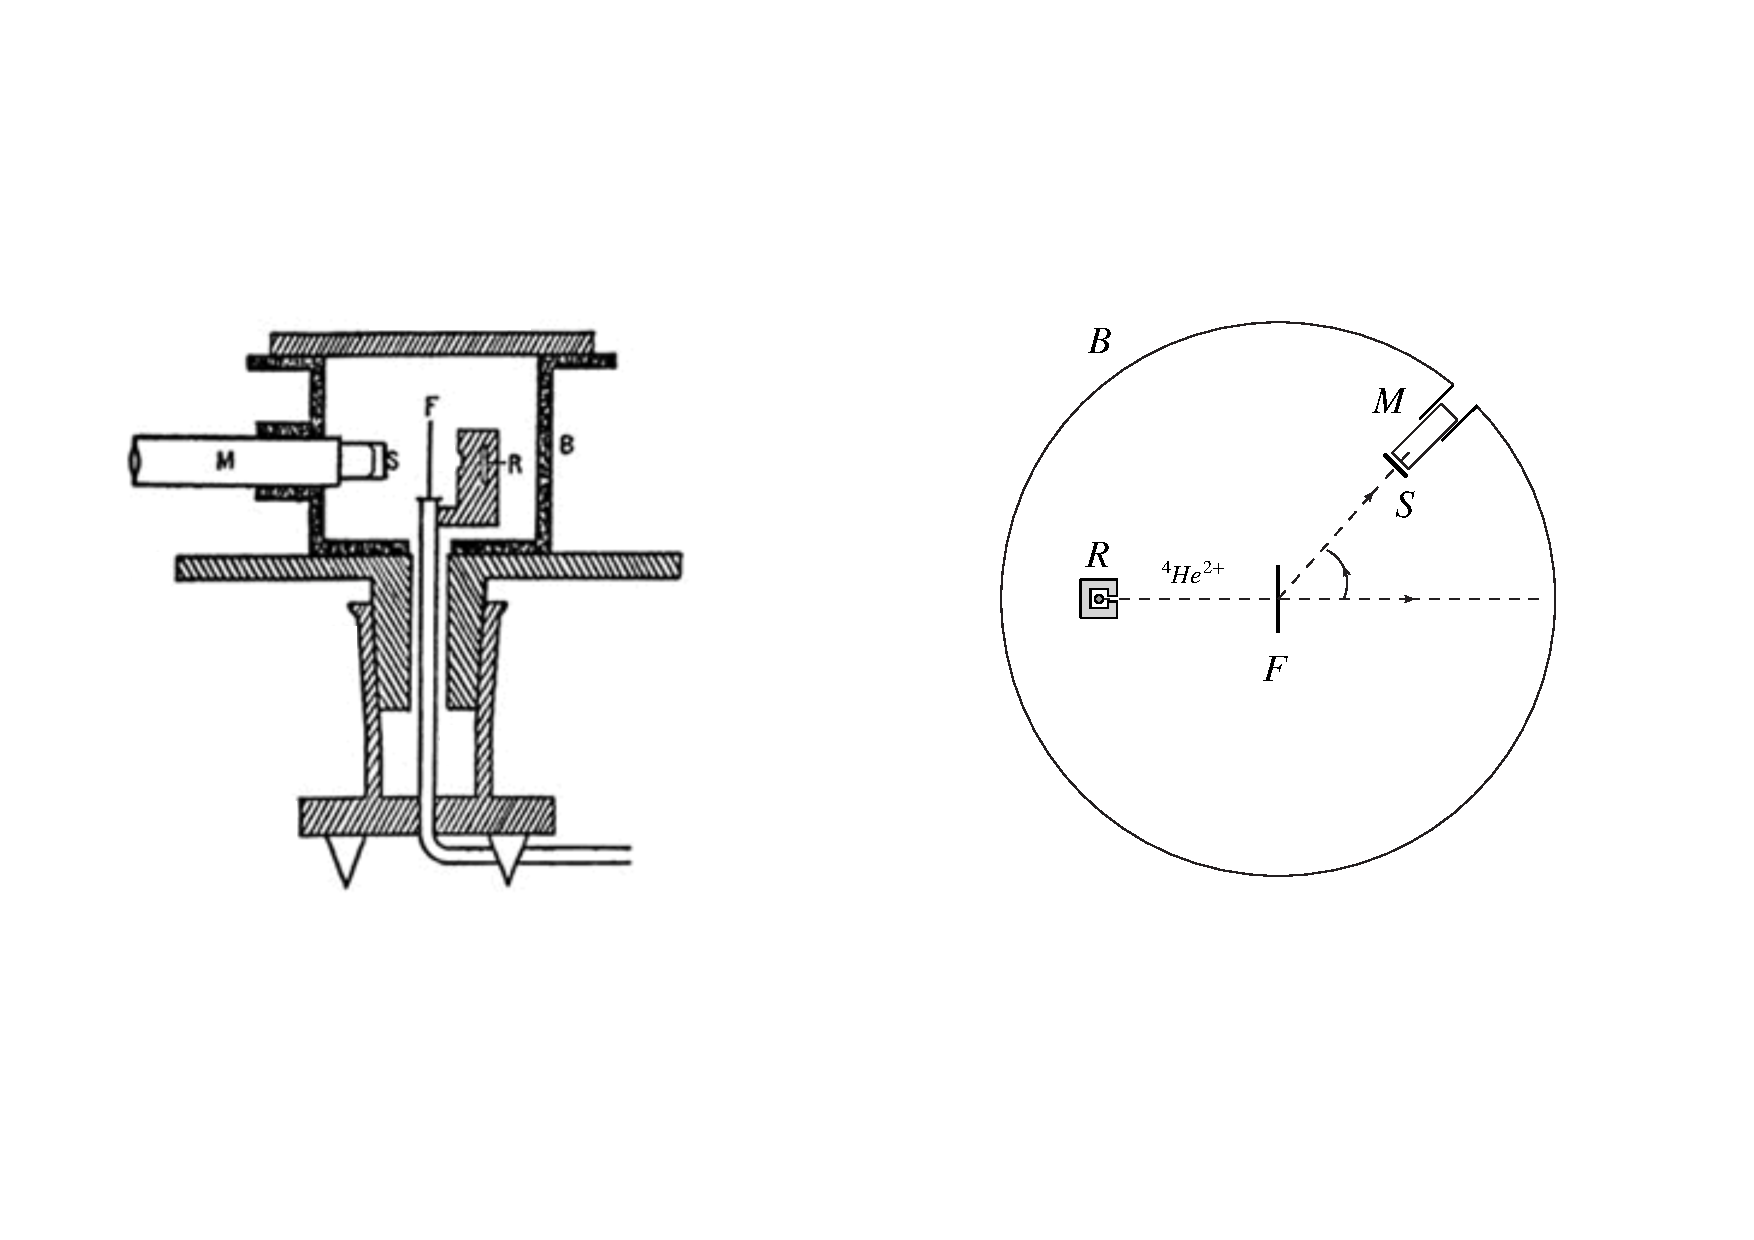
\includegraphics[width=0.9\textwidth]{Scattering-9}
    \caption{(Left) Illustration of the Rutherford-Geiger-Marsden $\alpha$ particles scattering experiment (lateral view). Source: Cambridge University. (Right) A schematic illustration of the principle of the experiment (top view) where the main points are reported:  (R) is the Radium source of $\alpha$ particles, (F) is the target foil, (M) is the microscope for the observation which could rotate along with the cylindrical box (B), (S) was a Zinc Sulfate screen which produced the scintillation at the passage of $\alpha$ particles to be observed by the microscope, and (D) a diaphragm through which the particles were emitted. }
    \label{fig:geiger-marsden}
\end{figure}{}

The result of the experiment was striking, as emphasized by Rutherford's famous quote: ``[The results were] as if you fired a 15-inch shell at a piece of tissue paper and it came back and hit you''. Back-scatterings of $\alpha$ particles were in fact observed.

\subsection{Prediction of the Rutherford Scattering Cross Section}
In order to explain the astonishing results of his scattering experiment, Rutherford proposed a different model for the atom where all the positive charges are concentrated in a small volume at the centre of the atom, and the negative particles (electrons) orbit around this central volume.

Assuming a relatively small volume for this ``nucleus'', when the $\alpha$ particle enters the volume of the atom, again -- according to Gauss' theorem -- the electric field created by the shell of electrons will cancel. The $\alpha$ particle will not ``feel'' the effect of the electrons, while the field from the ``nucleus'' (where the positive charges are concentrated) will act on the $\alpha$ particle as a point source, again according to Gauss' theorem (see the illustration of Rutherford's model in Fig.~\ref{fig:RutherfordAtom}).   
With this model greatly simplified by Gauss' theorem, the scattering cross section can be computed assuming that:
\begin{itemize}
    \item the scattering is elastic;
    \item the target is point-like, with a mass $M$ large with respect to the mass of the probe $\alpha$ particles, and with a charge $Ze$;
    \item the probe particle is $^4 He^{2+}$.
\end{itemize}
The scattering can be described schematically as in Fig.~\ref{fig:RutherfordScattering}, which represents the trajectory of a charged particle in a central potential. By construction it is known that these trajectories can be either open or closed, depending on the initial conditions of the system.

\begin{figure}
    \centering
    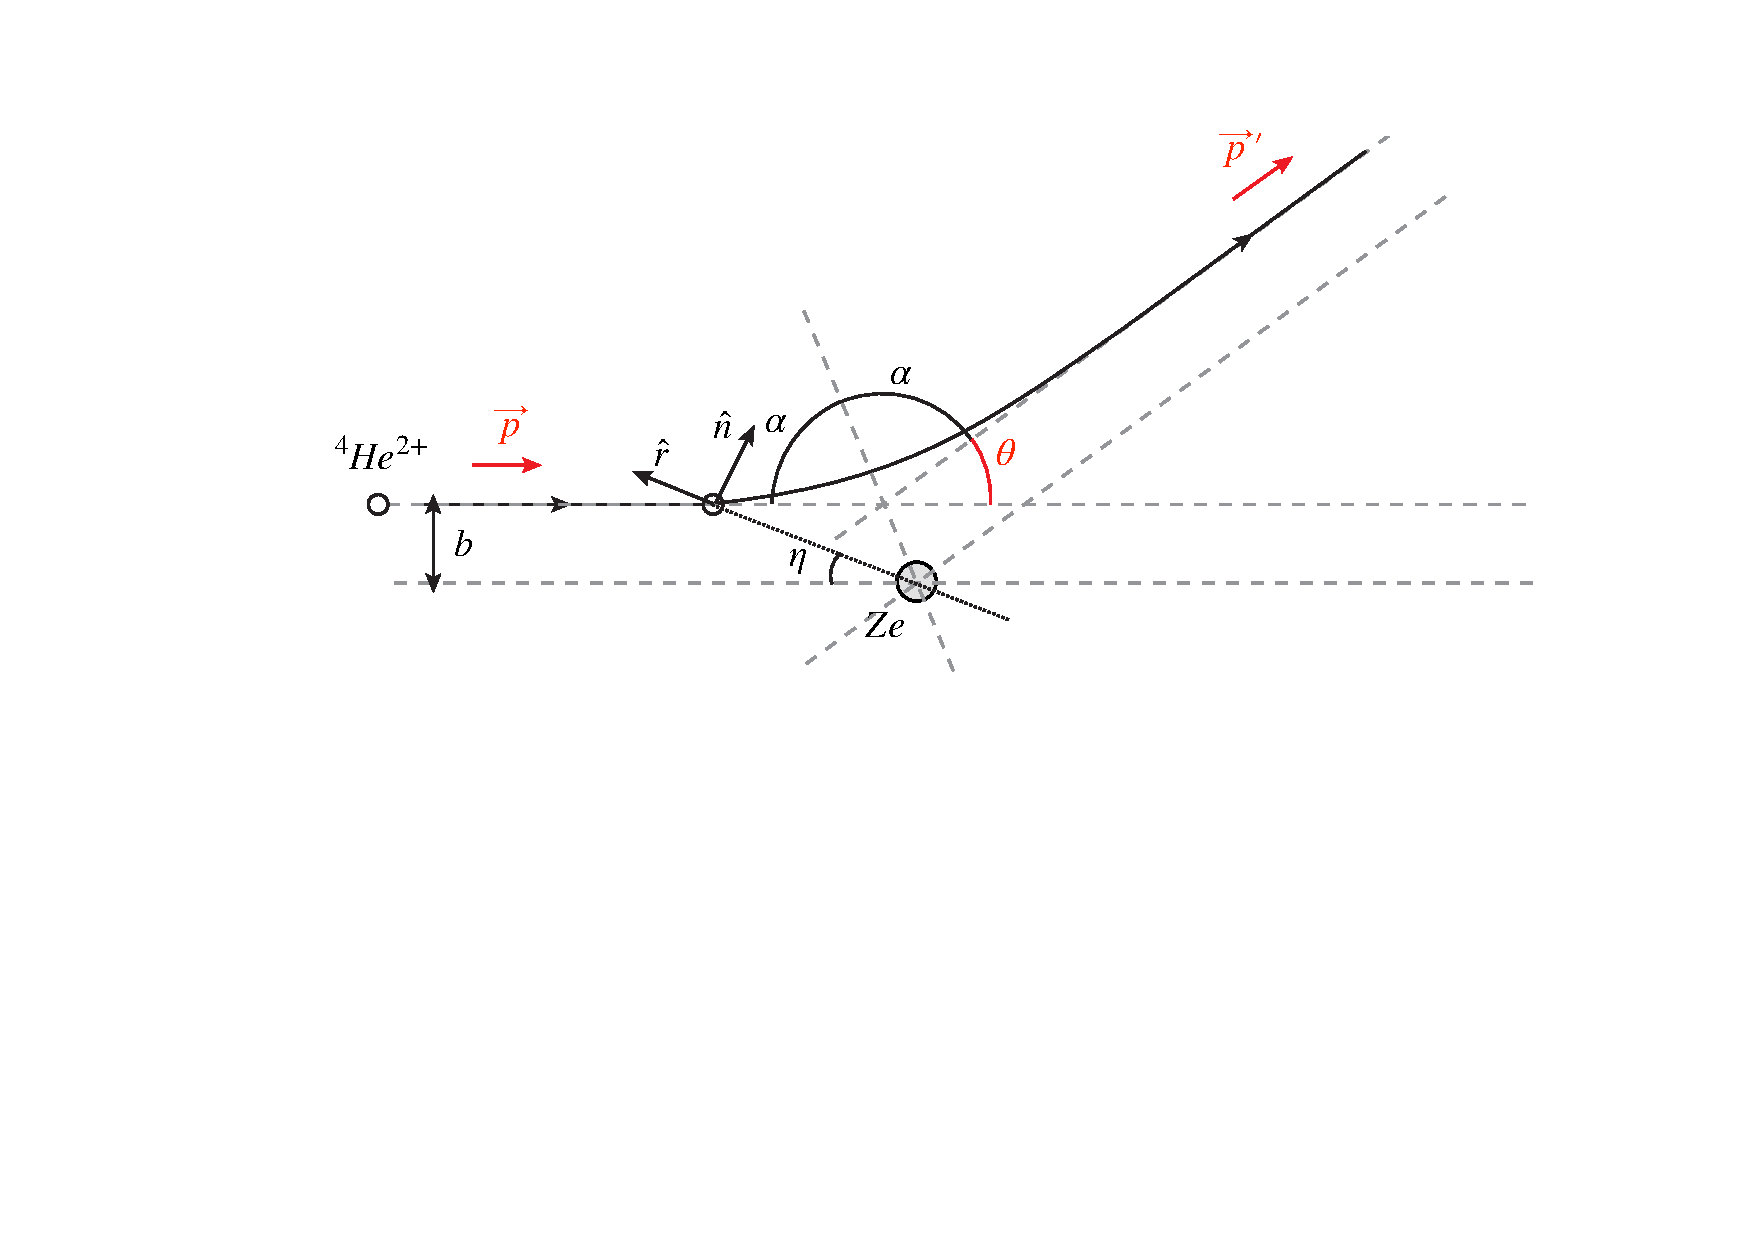
\includegraphics[width=1.0\textwidth]{Scattering-6}
    \caption{Illustration which shows the open hyperbolic trajectory of the $\alpha$ particles deviated from the Coulomb potential of the nucleus.
    In the image, $\theta$ denotes the scattering angle, $b$ the impact parameter of the incoming particle, $p$ is its momentum before the scattering, $p'$ is its momentum after the scattering and $Ze$ is the charge of the nucleus.}
    \label{fig:RutherfordScattering}
\end{figure}{}

In order to compute the cross section of this process, we need to stress an important conceptual point: we are facing a classical, non-relativistic problem which is fully deterministic. This implies that once the relation between the scattering angle and the impact parameter is known, the cross section will be known. The reasoning is precisely the same as that for the collision between hard spheres, where knowing the uniform distribution of the impact parameter probe particles, and using the relation between the impact parameter and the scattering angle, the differential cross section was known. 
The aim of the game will then be to \emph{find the relation between the impact parameter and the scattering angle}. In this case, the calculation will be a tad less straightforward than in the case of the hard spheres.

The first hypothesis is that we are dealing with a central potential,  i.e. that $V(r)$ has only a dependence in $r$. We will also assume that the potential is falling and becomes negligible (or at least its variations are negligible) at long distances. The Coulomb potential is in fact a good example of potential with such properties.
For the Coulomb potential, we know in advance that the trajectory will be a conic with a trajectory that can be open or closed, depending on the initial conditions of the system. As it will become clear in the following, we will be in the framework of an open hyperbolic trajectory. 

Let us define a coordinate system as described in Fig.~\ref{fig:RutherfordScattering}, which is centered in the scattering centre (i.e. the nucleus), which has been assumed to be point-like and is the origin of the potential. Let $\hat{r}$ be the radial unit vector along the direction of the probe particle (an $\alpha$ particle) to the target particle (nucleus); $\hat{n}$ is the normal unit vector. 

Given that the force generated by the potential on the probe particle is radial, its torque will be equal to $0$:
\[
\od{\vec{l}}{t} = \od{(\vec{r}\wedge\vec{p})}{t} = \od{r}{t}\hat{r}\wedge m\vec{v} + \vec{r}\wedge\od{\vec{p}}{t} = \vec{v}\wedge m\vec{v} + \vec{r}\wedge\vec{F} = 0.
\]
Therefore the angular momentum of the probe particle will be a constant of motion,
\[ \vec{\ell} = \vec{r} \wedge m \vec{v} \; \; {\rm thus} \; \; \ell = mrv \sin \eta, \]
where $\eta$ is the angle formed by the vectors $\vec{r}$ and $\vec{v}$. One can then calculate $\ell$ when the $\alpha$ particle is far away from the nucleus, i.e. when $V(r)\rightarrow 0$ and $r\sin\eta=b$, so that
\[
\ell = m r v \sin \eta = m b v_0,
\]
where $v_0$ is the velocity of the particle before scattering. Since energy is conserved, one has immediately

%The angle $\psi$ will relate to the angle $\eta$ through the following relation (see Fig.~\ref{fig:RutherfordScattering}:

%$$ \eta = \pi - \chi - \gamma$$

%Looking at the limit $\eta \rightarrow \pi$, assuming that the angle $\gamma$ will fall rapidly to 0 (which is the case since the electric field outside the atom will be expected to be exactly 0), then

%$$\lim\limits_{\eta \rightarrow \pi} \; |r \sin \eta| \sim r \sin \chi \sim b $$

%Therefore in terms of angular momentum:

%$$\lim\limits_{\eta \rightarrow \pi} \; \ell = \ell_0 = m v_0 b$$

%Where the initial velocity can be expressed in terms of the initial energy of the $\alpha$ particles $E$:

\begin{equation}
\label{eq:E}
E = \frac{1}{2} m v_0^2 \; \; \Rightarrow \; \; v_0 = \sqrt{\frac{2E}{m}}  \; \; \Rightarrow \; \; b^2 = \frac{\ell^2}{m^2v_0^2} = \frac{\ell^2}{2mE},
\end{equation}
i.e. we expressed the impact parameter in terms of conserved quantities, the angular momentum of the particle and its total energy, which are constants of motion.

Since the potential is central, it is convenient to represent the position of the incoming particle, $\vec{r}$, in polar coordinates. One has that $\vec{r}=(x,y)$, with
\[
\begin{cases}
x = r \cos \chi,\\
y = r \sin \chi,
\end{cases}
\]
where $\chi$ is the angle between the horizontal axis and $\vec{r}$. In other words, one has
\[
\vec{r}= r\cos\chi \hat{x}+r\sin\chi\hat{y} = r\hat{r},
\]
where $\hat{r}$ is the unit vector along the direction of $\vec{r}$. The unit vector orthogonal to $\hat{r}$ is
\[
\hat{n} = -\sin\chi \hat{x} + \cos\chi \hat{y},
\]
as it can be seen immediately by checking that $\hat{n}\cdot \hat{r}=0$. One can also note that
\[
\od{\hat{r}}{\chi} = \hat{n}.
\]
As a result, we can express the angular momentum of the particle as
\begin{equation*}
\begin{split}
\vec{l}&=m\vec{r}\wedge\vec{v} = m\vec{r}\wedge\od{\vec{r}}{t} = m\vec{r}\wedge\od{(r\hat{r})}{t}\\& = m\vec{r}\wedge\left[\od{r}{t}\hat{r}+r\od{\hat{r}}{t}\right] = 0+m\vec{r} \wedge \left[r\od{\hat{r}}{\chi}\od{\chi}{t}\right] = mr^2\hat{n}\od{\chi}{t},
\end{split}
\end{equation*}
i.e.
%We can then write for any position of the probe $\alpha$ particle on its trajectory that (in polar coordinates within the scattering plane):

%$$\ell = m |\vec{r} \wedge (\frac{dr}{dt} \hat{r} + r \frac{d\chi}{dt}\hat{n})| = mr^2 \frac{d\chi}{dt}$$

%Therefore we will have the following expression:

\begin{equation}
\label{eq:dchi}
\frac{d\chi}{dt} = \frac{\ell}{mr^2}.
\end{equation}

The source used by Rutherford was radium. The typical $\alpha$ radiation energy is of the order of 5~MeV. The total energy of the $\alpha$ particle will be
\[ E = T + m_{\alpha}c^2 = 4005 \; {\rm MeV} \; \Rightarrow \; \gamma = \frac{E}{m_{\alpha}} \sim 1.\]
The momentum of the $\alpha$ particle will then be
\[ p = \sqrt{E^2 - m_{\alpha}^2c^4} \sim 200 \; {\rm MeV/c} \; \Rightarrow \; \beta \gamma \sim \beta \sim 0.05.\]
The probe particle in the fixed-target reference frame is therefore in a  non-relativistic regime. 

The non-relativistic total energy, taking into account the central potential $V(r)$, can be written as
\[E = \frac{1}{2} m v^2 + V(r) = \frac{1}{2} m \left ( \frac{dr}{dt} \right )^2 + \frac{1}{2} m  r^2 \left ( \frac{d\chi}{dt} \right )^2 + V(r).\]
It is worth stressing the fact that $E$ is a constant of motion, while $V$ is a function of $r$.
From the previous expressions we obtain that
\[\frac{1}{2} m \left ( \frac{dr}{dt} \right )^2 = E - V(r) -\frac{\ell^2}{2mr^2} \; \; \Rightarrow \; \;\frac{dr}{dt} = - \sqrt{\frac{2}{m} \left ( E-V(r)-\frac{\ell^2}{2mr^2} \right )},\]
where we took the negative solution since $r$ decreases in the first phase of the trajectory. Using the expression of the angular momentum as a function of the impact parameter from Eq.~\eqref{eq:E}, we get
\begin{equation}
\label{eq:dr}
\frac{dr}{dt} = - \frac{\ell}{mrb} \sqrt{r^2 \left (1-\frac{V(r)}{E} \right ) - b^2}
\end{equation}

Given the expression of Eq.\ref{eq:dchi}, we can derive the variation of $d\chi$:
\begin{equation*}
\begin{split}
d\chi &= \frac{\ell}{mr^2}dt = \frac{\ell}{mr^2}\od{t}{r} dr \\&= \frac{\ell}{mr^2} \dfrac{dr}{-\dfrac{\ell}{mrb}  \sqrt{r^2 \left(1-\dfrac{V(r)}{E} \right) - b^2}} = \frac{-b dr}{r\sqrt{r^2\left(1-\frac{V(r)}{E}\right)-b^2}}.
\end{split}
\end{equation*}

In order to obtain an expression of the scattering angle $\theta$ as a function of the impact parameter of the particle, we consider the point of closest approach of the particle to the nucleus. In that point of space, denoted as $r=r_0$, the particle will have zero velocity, i.e.

\[
\left.\frac{dr}{dt}\right|_{r=r_0} = 0.
\]

This condition is satisfied if the argument of the square root of Eq. \eqref{eq:dr} vanishes, from which we get a relation between the impact parameter and the distance of closest approach,
\[r_0^2 \left ( 1 -\frac{V(r_0)}{E} \right ) - b^2 = 0.\]
This allows us to write
\[ \int_0^{\alpha} d\chi = \alpha = \int_{\infty}^{r_0} \frac{-b dr}{r \sqrt{r^2 \left (1-\dfrac{V(r)}{E} \right ) - b^2}},\]
where we used the fact that the particle comes from infinite distance ($\alpha=0$) and reaches $\alpha$ for $r=r_0$.

From the relation $2\alpha+\theta = \pi$ (which is evident from the symmetry\footnote{This is simply a consequence of the conservation of momentum of the incoming particle.} of  Fig.~\ref{fig:RutherfordScattering}), we get
\[\alpha = \frac{\pi}{2} - \frac{\theta}{2},\]
from which we obtain:
\begin{equation}
\label{eq:generalintegral}
\theta = \pi - 2b \int_{r_0}^{\infty} \frac{dr}{r \sqrt{r^2 \left (1-\dfrac{V(r)}{E} \right ) - b^2}}.
\end{equation}
This formula is valid for every scattering subject to a central potential $V(r)$.

Now let's use the fact the interaction between the $\alpha$ particle and the nucleus is given by the Coulomb potential. The $\alpha$ particle ($^4 He^{2+}$) has charge $z=2$, and we have
\[ V(r) = \frac{zZe^2}{4 \pi \varepsilon_0 r}.\]

In order to simplify the notation, let us define the constant $A = \dfrac{zZe^2}{4 \pi \varepsilon_0 E}$. Then the general central potential integral of Eq.~\eqref{eq:generalintegral} becomes
\begin{equation}
    \label{eq:coulombintegral}
    \theta = \pi - 2b \int_{r_0}^{\infty} \frac{dr}{r \sqrt{r^2 \left (1-\dfrac{A}{r} \right ) - b^2}}.
\end{equation}
We express the distance of closest approach for the Coulomb potential as
\begin{align}
    \left(1-\frac{A}{r}\right)r^2 = b^2\\
    r^2-Ar-b^2=0\\
    r=\frac{A\pm\sqrt{a^2+4b^2}}{2}=\frac{A}{2}\left(1 + \sqrt{1 + \frac{4b^2}{A^2}}\right)\equiv r_0,\label{eq:rutherfordclosestapproach}
\end{align}
where we took the physical solution of the second-order equation (positive sign before the square root).

To solve the integral of Eq.~\eqref{eq:coulombintegral}, we perform the change of variable $x=\frac{1}{r}$, i.e. $dx=-\frac{dr}{r^2}$. We obtain
\[ \theta = \pi - 2b \int_{r_0}^\infty \frac{-dx r^2}{r\sqrt{\frac{1}{x^2}\left(1-Ax\right)-b^2}} = \pi + 2b \int_{x_0}^{0} \frac{dx}{\sqrt{ 1 - A x - b^2 x^2}},\]
where we called $x_0=1/r_0$.

This integral can be computed from the general inverse trigonometric integral
\[ \int \frac{dx}{\sqrt{a +bx +cx^2}} = \frac{1}{\sqrt{-c}} \arccos \left ( -\frac{b+2cx}{\sqrt{b^2-4  ac}} \right ),\]
so that
\begin{equation}
    \label{eq:intacos}
     \theta = \pi + 2b \cdot \frac{1}{b} \left [ \arccos \left ( \frac{A+2b^2x}{\sqrt{A^2 + 4b^2}} \right ) \right ]_{x_0}^{0}
\end{equation}

The lower integration boundary $x_0$ can be written as
\[ x_0 =\frac{1}{r_0} = \frac{2}{A}\frac{1}{\left ( 1 + \sqrt{1 + \frac{4b^2}{A^2}} \right )}.\]
If we define $y = \frac{4b^2}{A^2}$, the argument of the $\arccos$ simplifies greatly:

$$ \frac{A+2b^2x_0}{\sqrt{A^2+4b^2}}=\frac{1+ \dfrac{y}{\left (1 + \sqrt{1+y} \right )}}{\sqrt{1+y}} = \frac{1 + \sqrt{1+y} + y}{\sqrt{1+y} + 1 + y} = 1.$$

Eq.~\eqref{eq:intacos} can then be written in a simple form, by evaluating the upper bound of the integral:
\[ \theta = \pi + 2 \left[ - 2\arccos(1)\right] + \arccos \left (\frac{1}{\sqrt{1+y}} \right ).\]
Taking the cosine and squaring the above expression yields
\[\cos ^2 \left ( \frac{\theta-\pi}{2}\right ) = \frac{1}{1+\dfrac{4b^2}{A^2}}= \sin ^2 \frac{\theta}{2},\]
from which we obtain
\[ \frac{4b^2}{A^2} = \frac{1-\sin ^2\frac{\theta}{2}}{\sin ^2 \frac{\theta}{2}} = \frac{\cos ^2\frac{\theta}{2}}{\sin ^2 \frac{\theta}{2}} = \frac{1}{\tan ^2 \frac{\theta}{2}},\]
therefore
\begin{equation}
\label{eq:ImpactParameterR}
b = \dfrac{A}{2} \dfrac{1}{\tan \dfrac{\theta}{2}} = \dfrac{zZe^2}{8 \pi \varepsilon_0 E \tan  \dfrac{\theta}{2}}.
\end{equation}

We have the relation between the impact parameter and the scattering angle, so we're almost there! As we have done for the scattering between hard spheres, the differential cross section can be written as:
\[d\sigma = 2\pi b db,\]
where $db$ is obtained from
\begin{equation}\label{eq:dbdthetainrutherford}\frac{db}{d\theta} = - \frac{1}{2} \frac{A}{2} \times  \frac{1}{\sin^2 \dfrac{\theta}{2}}.\end{equation}

Then, from
\[ d\sigma = 2 \pi b \left | \frac{db}{d\theta} \right | d\theta, \]
and using the fact that from the cylindrical symmetry of the scattering one has $d\Omega = 2\pi \sin \theta d\theta$, we can then write
\[\od{\sigma}{\Omega} = \frac{b}{\sin \theta} \od{b}{\theta} = \left ( \frac{A}{2} \right )^2 \frac{\dfrac{1}{\sin ^2 \dfrac{\theta}{2}}}{2 \sin \theta \tan \dfrac{\theta}{2}},\]
where we used Eq. \eqref{eq:ImpactParameterR} and Eq. \eqref{eq:dbdthetainrutherford}. Since $\sin \theta = 2 \sin \frac{\theta}{2} \cos \frac{\theta}{2}$, we obtain the differential cross section
\begin{equation}
    \label{eq:rutherford}
    \boxed{
    \frac{d\sigma}{d\Omega} =\left ( \frac{zZe^2}{16 \pi \varepsilon_0 E_k} \right )^2 \times \frac{1}{\sin^4 \dfrac{\theta}{2}}}
\end{equation}

\noindent where we have added the subscript $k$ to the energy term $E_k$ to make it clear that the energy involved here is the kinetic energy.

\subsection{Total cross section}
If one tries to calculate the total Rutherford cross section, by integrating Eq.~\eqref{eq:rutherford} in $d\Omega$, one would get a divergent result. This is a consequence of the fact that the interaction which is responsible for the scattering, the Coulomb interaction, is long-ranged: even a particle far away from the nucleus would ``feel'' the Coulomb force, and so contribute to the total scattering cross-section (even if very mildly). One can avoid this issue by applying a cut-off to the integration, i.e. considering a minimum, finite angle to which the integration stops. Also, the cross-section formula itself isn't fully valid for arbitrarily high impact parameter values, as they correspond to the $\alpha$ particle traveling beyond the last electron level, which would imply that the nuclear charge is screened by the atomic electrons, invalidating the hypotheses of our calculation.

\subsection{Interpretation}
\label{sec:RutherfordInterpretation}
The first important note is that this scattering cross section can be computed in a purely classical fashion. We will see in Chapter~\ref{scattering-2} that a similar result can be obtained in a straightforward fashion in a Quantum Mechanical approach. This could therefore be done before all the tools of quantum scattering were in place. \\

The Rutherford experiment has revolutionized our understanding of the atom and proved the existence of the atomic nucleus. The first striking consequence is the existence of a nucleus {\it per se}, a small volume that contains all the positive charges and most of the mass of the atom. This is an incredibly far-reaching consequence, as it implies that a strong force must exist which on one side is able to keep its positive constituents together, but at the same time has no impact on the scattering of the $\alpha$ particles -- at least at the scales that are observed by similar experiments (relatively low energies). \\

It is of course very important to increase the energy of the incoming particle to further investigate shorter distances (as discussed in Chapter~\ref{chap:Introduction}), and see up to which distance scales these conclusions hold. A more recent experiment using $\alpha$ particles with energies of up to \SI{40}{MeV} on a lead target is shown in Fig.~\ref{fig:RutherfordScatteringBreakdown} and can be found in Ref.~\cite{RutherfordScattering}. It is very interesting to note that the data follow accurately the Rutherford formula up to a point where the agreement breaks down and the influence of the nucleus becomes clear. This implies that the strong nuclear force binding the nucleus together should be short-ranged. The approximate size of the nucleus can then be inferred from the energy of the breakdown, by simply taking the formula of the impact parameter (Eq.~\eqref{eq:ImpactParameterR}), and considering a break-down kinetic energy of approximately $E = 28$~MeV and the classical radius of the electron $r_e \approx 2.82$~fm:
\[
r_{nucleus} \sim \dfrac{zZ r_e m_e c^2}{2 E \tan \frac{\theta}{2}} = 7.3~{\rm MeV}.
\]
Above this kinetic energy the impact parameter is such that the nuclear effects cannot be neglected! \\

\begin{figure}
    \centering
    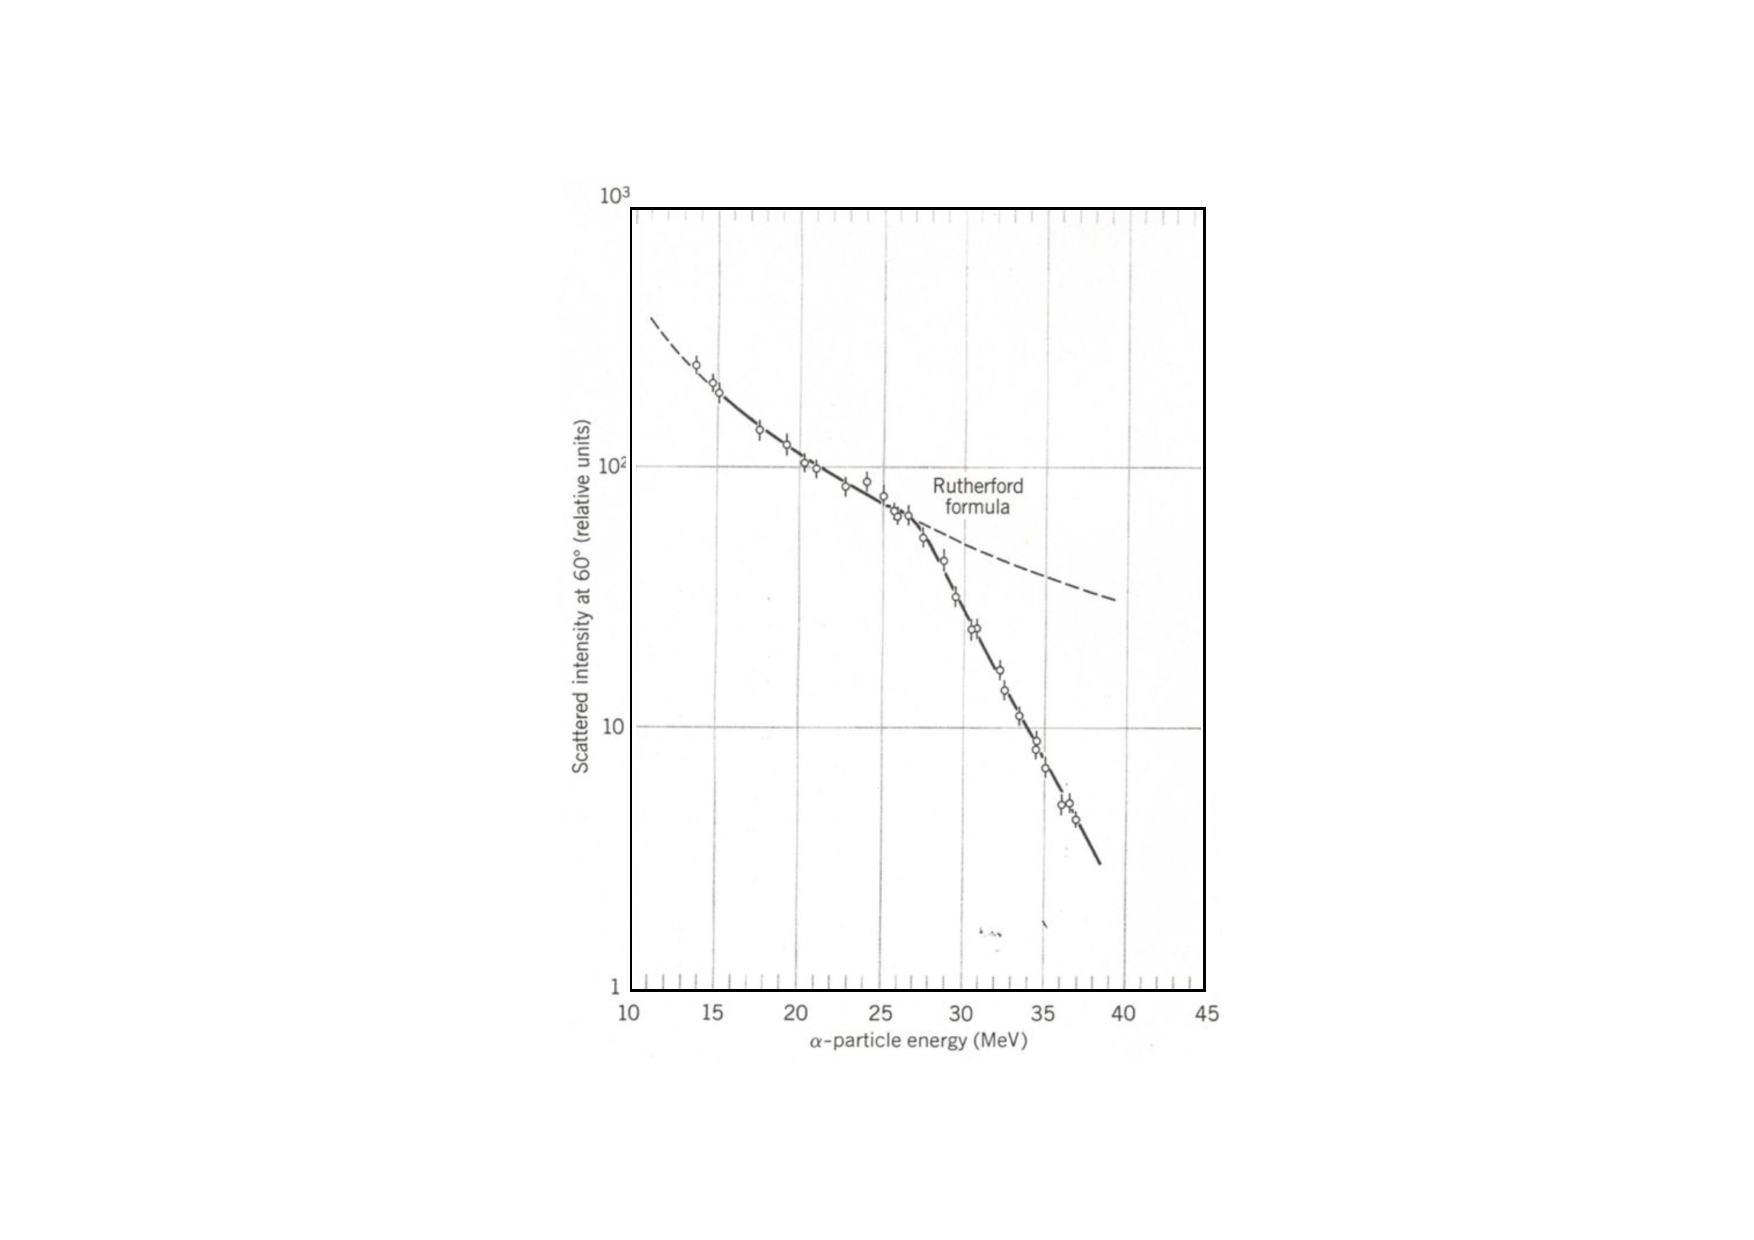
\includegraphics[width=0.65\textwidth]{R-Scattering}
    \caption{Measurement of the Rutherford cross section at a scattering angle of $\theta = 60^o$ with probe $\alpha$ particles with kinetic energy of up to approximately 40~MeV.}
    \label{fig:RutherfordScatteringBreakdown}
\end{figure}{}

These findings are crucial in building a theory of the interaction that holds the nucleus together, that will be referred to as the strong (nuclear) interaction -- as will be discussed in Chapter~\ref{chap:fundInteractions}. \\

Beyond giving a revolutionary picture of the atom (and now the nucleus), the formalism discussed in this section to derive the Rutherford formula will be used to discuss the interaction of particles in matter in Chapter~\ref{chap:InteractionsInMatter}.


\section*{Take-home lessons}
\begin{itemize}
    \item Scattering is an essential tool for studying the structure of molecules, atoms, nuclei and particles, and to study their properties and interactions. Scattering processes typically involve a particle being sent on a target, or two beams of particles scattering together.
    \item Elastic scattering is a scattering process in which the nature and number of the particles in the initial and final state are the same. Particles change only direction and energy, and the total kinetic energy is conserved.
    \item One basic concept for a quantitative description of scattering is that of \emph{impact parameter}. In classical scattering, for example when one rigid sphere undergoes elastic scattering with another sphere, impact parameter -- the distance between the centers of the two spheres -- fully determines the scattering angle (which is the angle at which the impinging sphere is deflected).
    \item In reality, scattering cannot be simply represented as the scattering of two rigid spheres. First of all, experiments typically involve a beam of particles colliding against some physical target, i.e. it's experimentally impossible to measure the motion of all single particles. Then, quantum mechanics states it's inherently impossible to know with arbitrary precision position and momentum of those particles. 
    \item In the case of a beam colliding over a fixed target, for example, one therefore needs to describe scattering by taking into account that the beam is composed by $N_A$ particles which travel its transverse surface $S$ with a flux $\phi_A=\od{N_A}{t}\frac{1}{S}$. The target is typically made of some physical material with $n_B$ target particles per unit of volume: if its length along the beam path is $d$, then the number of target particles seen by the beam is $N_B=n_b S d$.
    \item The ultimate question of scattering theory is: how many interactions $N_I$ between particles in the beam and particles in the target will happen in unit time, i.e. what is the scattering rate? In the case of a beam-target experiment, this rate is proportional to the flux of incoming particles and to the number of target particles seen by the beam, $\od{N_I}{t}=\sigma \phi_A N_B$. The proportionality factor $\sigma$ is called \emph{cross section}. Luminosity is instead defined as the product $\mathcal{L}=\phi_A N_B$.
    \item The cross section of a scattering process is a measure of the probability of that process to take place. Although cross section has the dimensions of the square of a length, it should not be interpreted as a measure of the relative physical size of the target with respect to the beam, like it is in the classical case of colliding rigid spheres.
    \item Luminosity is a property of the chosen experimental setup, not of the underlying interaction. One may in fact use different experimental setups -- for example, beam-target and beam-beam experiments -- to investigate the same scattering process. The interaction rate would then still be the product of cross section and luminosity.
    \item The density $n_B$ is the volume density of target particles in the physical target. Its role depends on which process one is considering: for example, in a scattering process between an electron beam and protons in a fixed, $n_B$ would be the number of protons in the atoms of the physical target, which can be expressed as a function of the atomic number, atomic mass and density of the target material.
    \item In real life one measures the position and energy of particles -- sometimes of all initial and final state particles, sometimes only of a few of them. Experiments are in general sensitive to \emph{differential} rates of interaction, which means that one measures how many particles are observed in unit time in a given portion of the solid angle, and/or how many of them have energy inside a given range. The differential interaction rate depends on the concept of differential cross section, which encloses the dependence of the interaction probability on quantities like the scattering angle and the particle energy. The integral of the differential cross section over those quantities gives of course the total cross section $\sigma$.
    \item How much a beam of particles can penetrate a fixed target is a function of the density of the target, and of the cross section of the interaction between beam and target particles. This process is inherently exponential, and is described by the absorption coefficient and its reciprocal, the attenuation length or mean free path.
    \item The Rutherford experiment proved that Thomson was wrong: atoms aren't uniformly filled with positive and negative charges, but rather they are made of small, positively-charged nuclei, around which negative electrons orbit. Rutherford sent a collimated beam of $\alpha$ particles on a thin gold target, and measured an interaction rate with a strong dependence on the scattering angle, compatible with the hypothesis of a sphere with a positive, small nucleus.
    \item The Rutherford experiment can be treated with a purely classical formalism, under the assumption that the $\alpha$ particle -- an helium nucleus -- undergoes an elastic scattering with the point-like gold nucleus, with which it interacts electromagnetically. The interaction potential which describes the interaction is therefore the Coulomb potential, which is central. The key to calculate  the differential interaction cross-section is finding the relation between the impact parameter and the scattering angle.
\end{itemize}
\section*{Questions}
\begin{itemize}
    \item What are the hypotheses which allow us to express impact parameter as a function of scattering angle, in Rutherford scattering?
    \item Are we really worried about the possible divergence of the Rutherford cross section at small angles?
    \item What would change in the Rutherford experiment if the atomic nucleus was negatively-charged? Can you think of a way to determine the charge of the nucleus?
\end{itemize}

\begin{thebibliography}{99.}%

\bibitem{RutherfordScattering} Eisberg, R. M. and Porter, C. E., Scattering of Alpha Paricles, Rev. Mod. Phys. 33, 190 (1961)

\end{thebibliography}

%\chapter{Elements of Scattering Theory - Part II }


\section{Quantum Mechanical Processes} 
\label{scattering-2}

\subsection{The Schr\"odinger Equation}

In quantum mechanics a system is described mathematically by its wave function. The interpretation of the wave function is a complex probability amplitude from which probabilities of outcomes of measurements can be inferred. 

In simpler terms, quantum mechanics postulates that a {\bf free particle} is described by the free Schr\"odinger equation.

The Schr\"odinger equation was formulated in 1925 by Erwin Schr\"odinger and published one year later. For postulating this equation Erwin Schr\"odinger was awarded the Nobel prize in 1933.


The Schr\"odinger's equation is inherently \emph{non-relativistic}. This can be deduced using the operators substitution in the non relativistic energy expression,

    \begin{equation}
        E = \frac{p^2}{2m}.
        \label{eq:classical-energyunpert}
    \end{equation}

Using the relations $E = i\hslash\frac{\partial}{\partial t}$ and $\Vec{p} = -i\hslash\Vec{\nabla}$, which can be summarized in Einstein's notation as

\begin{equation}
\boxed{p_{\mu} = i\hslash \partial_{\mu},}
\end{equation}
then Eq. \eqref{eq:classical-energyunpert} becomes
    \begin{equation}
        -\frac{\hslash^2}{2m}\nabla^2\psi = i\hslash\frac{\partial}{\partial t}\psi.
        \label{eq:schroedinger1unpert}
    \end{equation}

In quantum-mechanical terms, the goal of a scattering experiment is the study of a localized and stationary (time-independent) potential, $V(x)$. Here \emph{localized} implies that $V(x) \rightarrow 0$ when $x \rightarrow \pm \infty$.

For the sake of simplicity, let us just consider the one-dimensional case. The idea is to imagine the scattering experiment as a quantum particle traveling along the $x$-direction and encountering the potential. The equation of motion is governed by the Schr\"odinger equation,

\begin{equation}
\label{eq:schrodinger}
 -\frac{\hslash^2}{2m} \frac{\partial^2 \psi}{\partial x^2} + V(x) \psi =  i\hslash \frac{\partial \psi}{\partial t}.
\end{equation}

The solutions to the Schr\"odinger equation in a single spatial dimension are the {\bf energy eigenstates}
\[\psi(x,t) = e^{\pm \frac{iEt}{\hslash}}\psi(x),\]
where it is clear the separation of the overall wavefunction as the product of a time-dependent and a position-independent term. This holds only if the potential is stationary, i.e. $V=V(x)$.

Negative-energy solutions yield bound states\footnote{This is true only for the Schr\"odinger equation, while the case of a relativistic particle will be different and discussed for the Klein-Gordon equation.}.This can be easily seen with any shape of a one-dimensional potential $V(x)$ where it is assumed that the potential is constant at $x \rightarrow \pm \infty$, meaning that the particle is free far from the region where the potential acts (a typical, reasonable assumption in a scattering experiment). 

Then, by fixing the value of the potential at $x=\pm\infty$ to $0$, it can be seen that initial negative energies will be bound in the region of $x$ where the potential acts ($[x_1,x_2]$), and the particle will oscillate between $x_1$ and $x_2$. Instead, if the initial energy is positive, $E>0$ then a free particle starting from the left with momentum $p$ will be only perturbed by the potential and will then recover its momentum when traveling away from the potential. 

The classification discussed above is interesting, and one could wonder whether in all cases bound states will not appear, even when there is some ``hole'' in the potential. However, even if there is a hole in the potential, the solutions to the Schr\"odinger equation will still be scattering solutions, as the system will be able to tunnel out of the ``hole'' with some non-zero probability.

\subsection{Normalization of the wave function}

In order to be able to interpret the wave function as a description of a physical particle, one needs to consider the problem of its normalisation. From a mathematical point of view, the solutions of the Schr\"odinger equation allow for any normalisation to be chosen; however, this results in different physical interpretations of the meaning of those wave functions.

Let's consider the case of a free particle, which can be described by a plane wave
    \begin{equation}
        \psi = Ne^{i\Vec{p}\cdot\Vec{x}-i\frac{p^2}{2m}t},
    \end{equation}
which solves the Schr\"odinger equation; $N$ is a normalisation factor. Given the probabilistic interpretation of the wave function, a value of \(N\neq1\) implies that a given volume $V$ contains $N^2$ particles,

\begin{equation}
    \int_V | \psi^* \psi| dV = N^2 \times V.
\end{equation}

While the wave function normalisation is a matter of convention, it is important that the physical predictions -- namely, the cross section of a scattering process -- are independent of this choice. Often the choice will be
\begin{equation*}
    \int_V | \psi^* \psi| dV = 1,
\end{equation*}
in which case the wave function will simply be
\begin{equation*}
    \psi = e^{i\Vec{p}\cdot\Vec{x}-i\frac{p^2}{2m}t}.
\end{equation*}

The problem is that, when one considers an infinite volume, it is not possible to fix the wave function normalisation from the normalisation of the total probability (or probability density),%, the probability current is not possible (
as it means that $N^2 \rightarrow 0$. The normalisation of the wave function from the total probability is possible when one considers the free particle not as a single wave function, but rather as a \emph{superposition of plane waves}, i.e. a \emph{wave packet}, which can be written as a Fourier decomposition
   \begin{equation}
        \psi(x) = \int \psi(k) e^{ikx} dk,
    \end{equation}
where
   \begin{equation}
        \psi(k) = \int \psi(x) e^{-ikx} dx.
    \end{equation}

A useful representation of the wave packet is the \emph{Gaussian wavepacket}, which is Gaussian both in momentum and position space and gives a good approximation of the Heisenberg uncertainty relation. For the purpose of these note, we will avoid to enter into the details of this more precise description of a \textbf{quantum particle}.

\subsection{Probability current}

The complex conjugate Schr\"odinger equation can be written as

    \begin{equation}
        -i\frac{\partial}{\partial t}\psi^* + \frac{\hslash}{2m}\nabla^2\psi^* = 0.
        \label{eq:schroedinger2}
    \end{equation}
    
    Multiplying Eq. \eqref{eq:schroedinger1unpert} by $\psi^*$ and Eq. \eqref{eq:schroedinger2} by $\psi$ (on the left side), we obtain
    \begin{equation*}
        i\psi^*\frac{\partial\psi}{\partial t} + \frac{\hslash}{2m}\psi^*\nabla^2\psi = 0, 
    \end{equation*}
    and
    \begin{equation*}
        -i\psi\frac{\partial\psi^*}{\partial t} + \frac{\hslash}{2m}\psi\nabla^2\psi^* = 0.
    \end{equation*}
    Subtracting the two equations we obtain
    \begin{equation*}
        i\left(\psi^*\frac{\partial\psi}{\partial t}+\psi\frac{\partial\psi^*}{\partial t}\right) + \frac{\hslash}{2m}\left(\psi^*\nabla^2\psi - \psi\nabla^2\psi^*\right) = 0,
    \end{equation*}
    which becomes
    \begin{equation}
        i\frac{\partial}{\partial t}(\psi^*\psi) + \frac{\hslash}{2m}\Vec{\nabla}\cdot(\psi^*\Vec{\nabla}\psi - \psi\Vec{\nabla}\psi^*) = 0.
        \label{eq:density-prob-continuity}
    \end{equation}
    The quantity $\rho = \psi^*\psi$ is the probability density. Equation \ref{eq:density-prob-continuity} is the usual continuity equation.
    
    If we consider a volume $V$, the variation of probability in the volume can be expressed as 
    \begin{equation*}
        \delta p = \frac{\partial}{\partial t}\iiint_{V} \rho\,dV.
    \end{equation*}
    If we call $\Vec{j}$ the vector of the probability current, we can write the probability flux through a surface element $\Vec{ds}$ as $\Vec{j}\cdot\Vec{dS}$ (as shown in Figure \ref{fig:probability-current}. We exploit the divergence theorem to write
    \begin{equation*}
        \frac{\partial}{\partial t}\iiint_{V} \rho \,dV = -\oiint_{S} \Vec{j}\cdot\Vec{dS} = \iiint_V \Vec{\nabla}\cdot\Vec{j} \,dV.
    \end{equation*}
    \begin{figure}
        \centering
        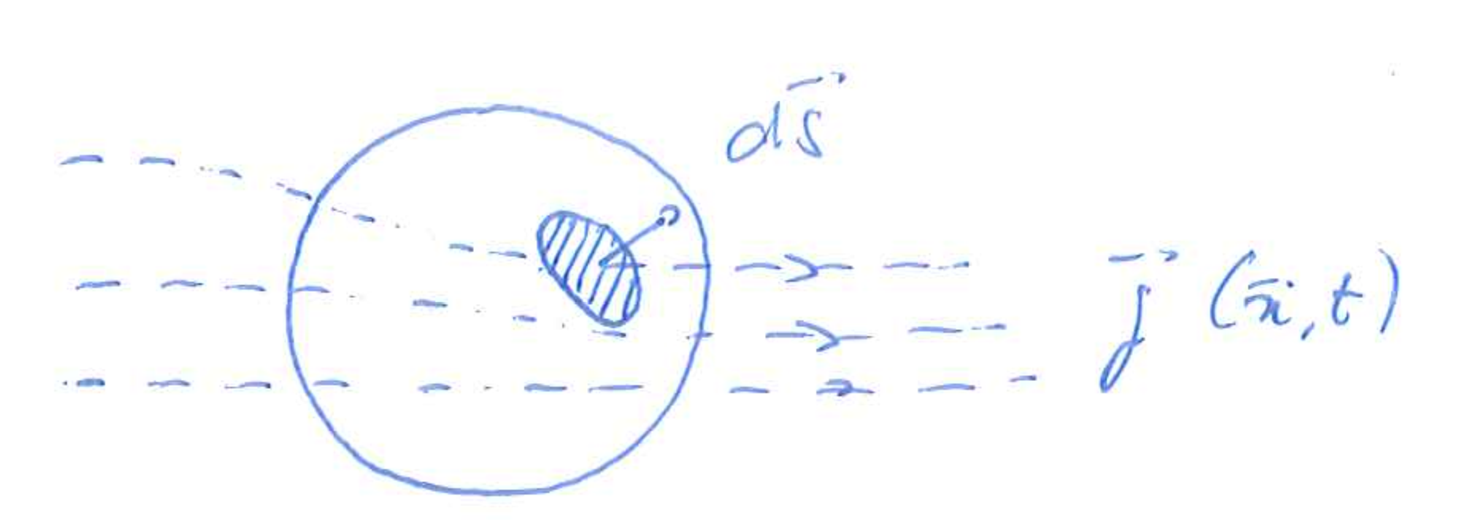
\includegraphics[width=0.7\textwidth]{Figures/probability-current}
        \caption{Representation of the probability flux.}
        \label{fig:probability-current}
    \end{figure}
    This equations holds for each arbitrary choice of $V$, therefore we can write
    \begin{equation*}
        \frac{\partial}{\partial t}\rho + \Vec{\nabla}\cdot\Vec{j} = 0,
    \end{equation*}
    and identify this probability current with the expression of Eq. \eqref{eq:density-prob-continuity}, obtaining
    \begin{equation*}
        \Vec{j} = \frac{\hslash}{2mi}\left(\psi^*\Vec{\nabla}\psi - \psi\Vec{\nabla}\psi^*\right).
    \end{equation*}
    
    If we take the free-particle wave function and choose to normalise it by $N$, where $N^2$ has the meaning of number of particles in a volume $V$, then we  have $\rho = \psi^*\psi = N^2$, and the current $\Vec{j}$ will be  given by
    \begin{equation*}
        \Vec{j} = \frac{1}{2mi}\left(\psi^*(i\Vec{p}\psi)-\psi(i\Vec{p})\psi^*\right) = \frac{\Vec{p}}{2m}2\left|\psi\right|^2 = \frac{\Vec{p}}{m}\left|\psi\right|^2 = \Vec{v}\cdot \rho,
    \end{equation*}
    where we used \(\Vec{p}=-i\hslash\Vec{\nabla}\) and \(\nabla\psi^*=(\nabla\psi)^*=(\frac{\Vec{p}}{i\hslash}\psi)^*=\frac{\Vec{p}}{-i\hslash}\psi^*\).
    We can conclude that, since $\rho = |N|^2$ is the density (number of particles per unit volume),  then $\Vec{j} = \rho\Vec{v}$ is the flux of particles through an unit arc in a unit time. We will see that this is the same expression as defined in the cross section formula calculation with the Fermi's golden rule.


\subsection{Time independent formalism, the one dimensional case}

Let us consider the case of a generic (stationary) potential $V(x)$, such as the one illustrated in Figure~\ref{fig:potential-1}, and a system consisting of a particle in one dimension. The  Schr\"odinger equation is a second order differential equation and has two generic solutions, which correspond to the particle moving from right to left or from left to right. The possible states at infinity, which would correspond to the initial and final states being free particles, will have energy

\[ E = \frac{\hslash^2 k^2}{2m}.\]

The scattering states (i.e. those with $E>0$) give rise to solutions that can be right-moving, $e^{ikx}$, or left-moving, $e^{-ikx}$.\footnote{We must stress that, since the Hamiltonian is time-independent by hypothesis, here we are not talking about time dependence at all: the state of the system does not evolve in time.}

    \begin{figure}
%        \centering
        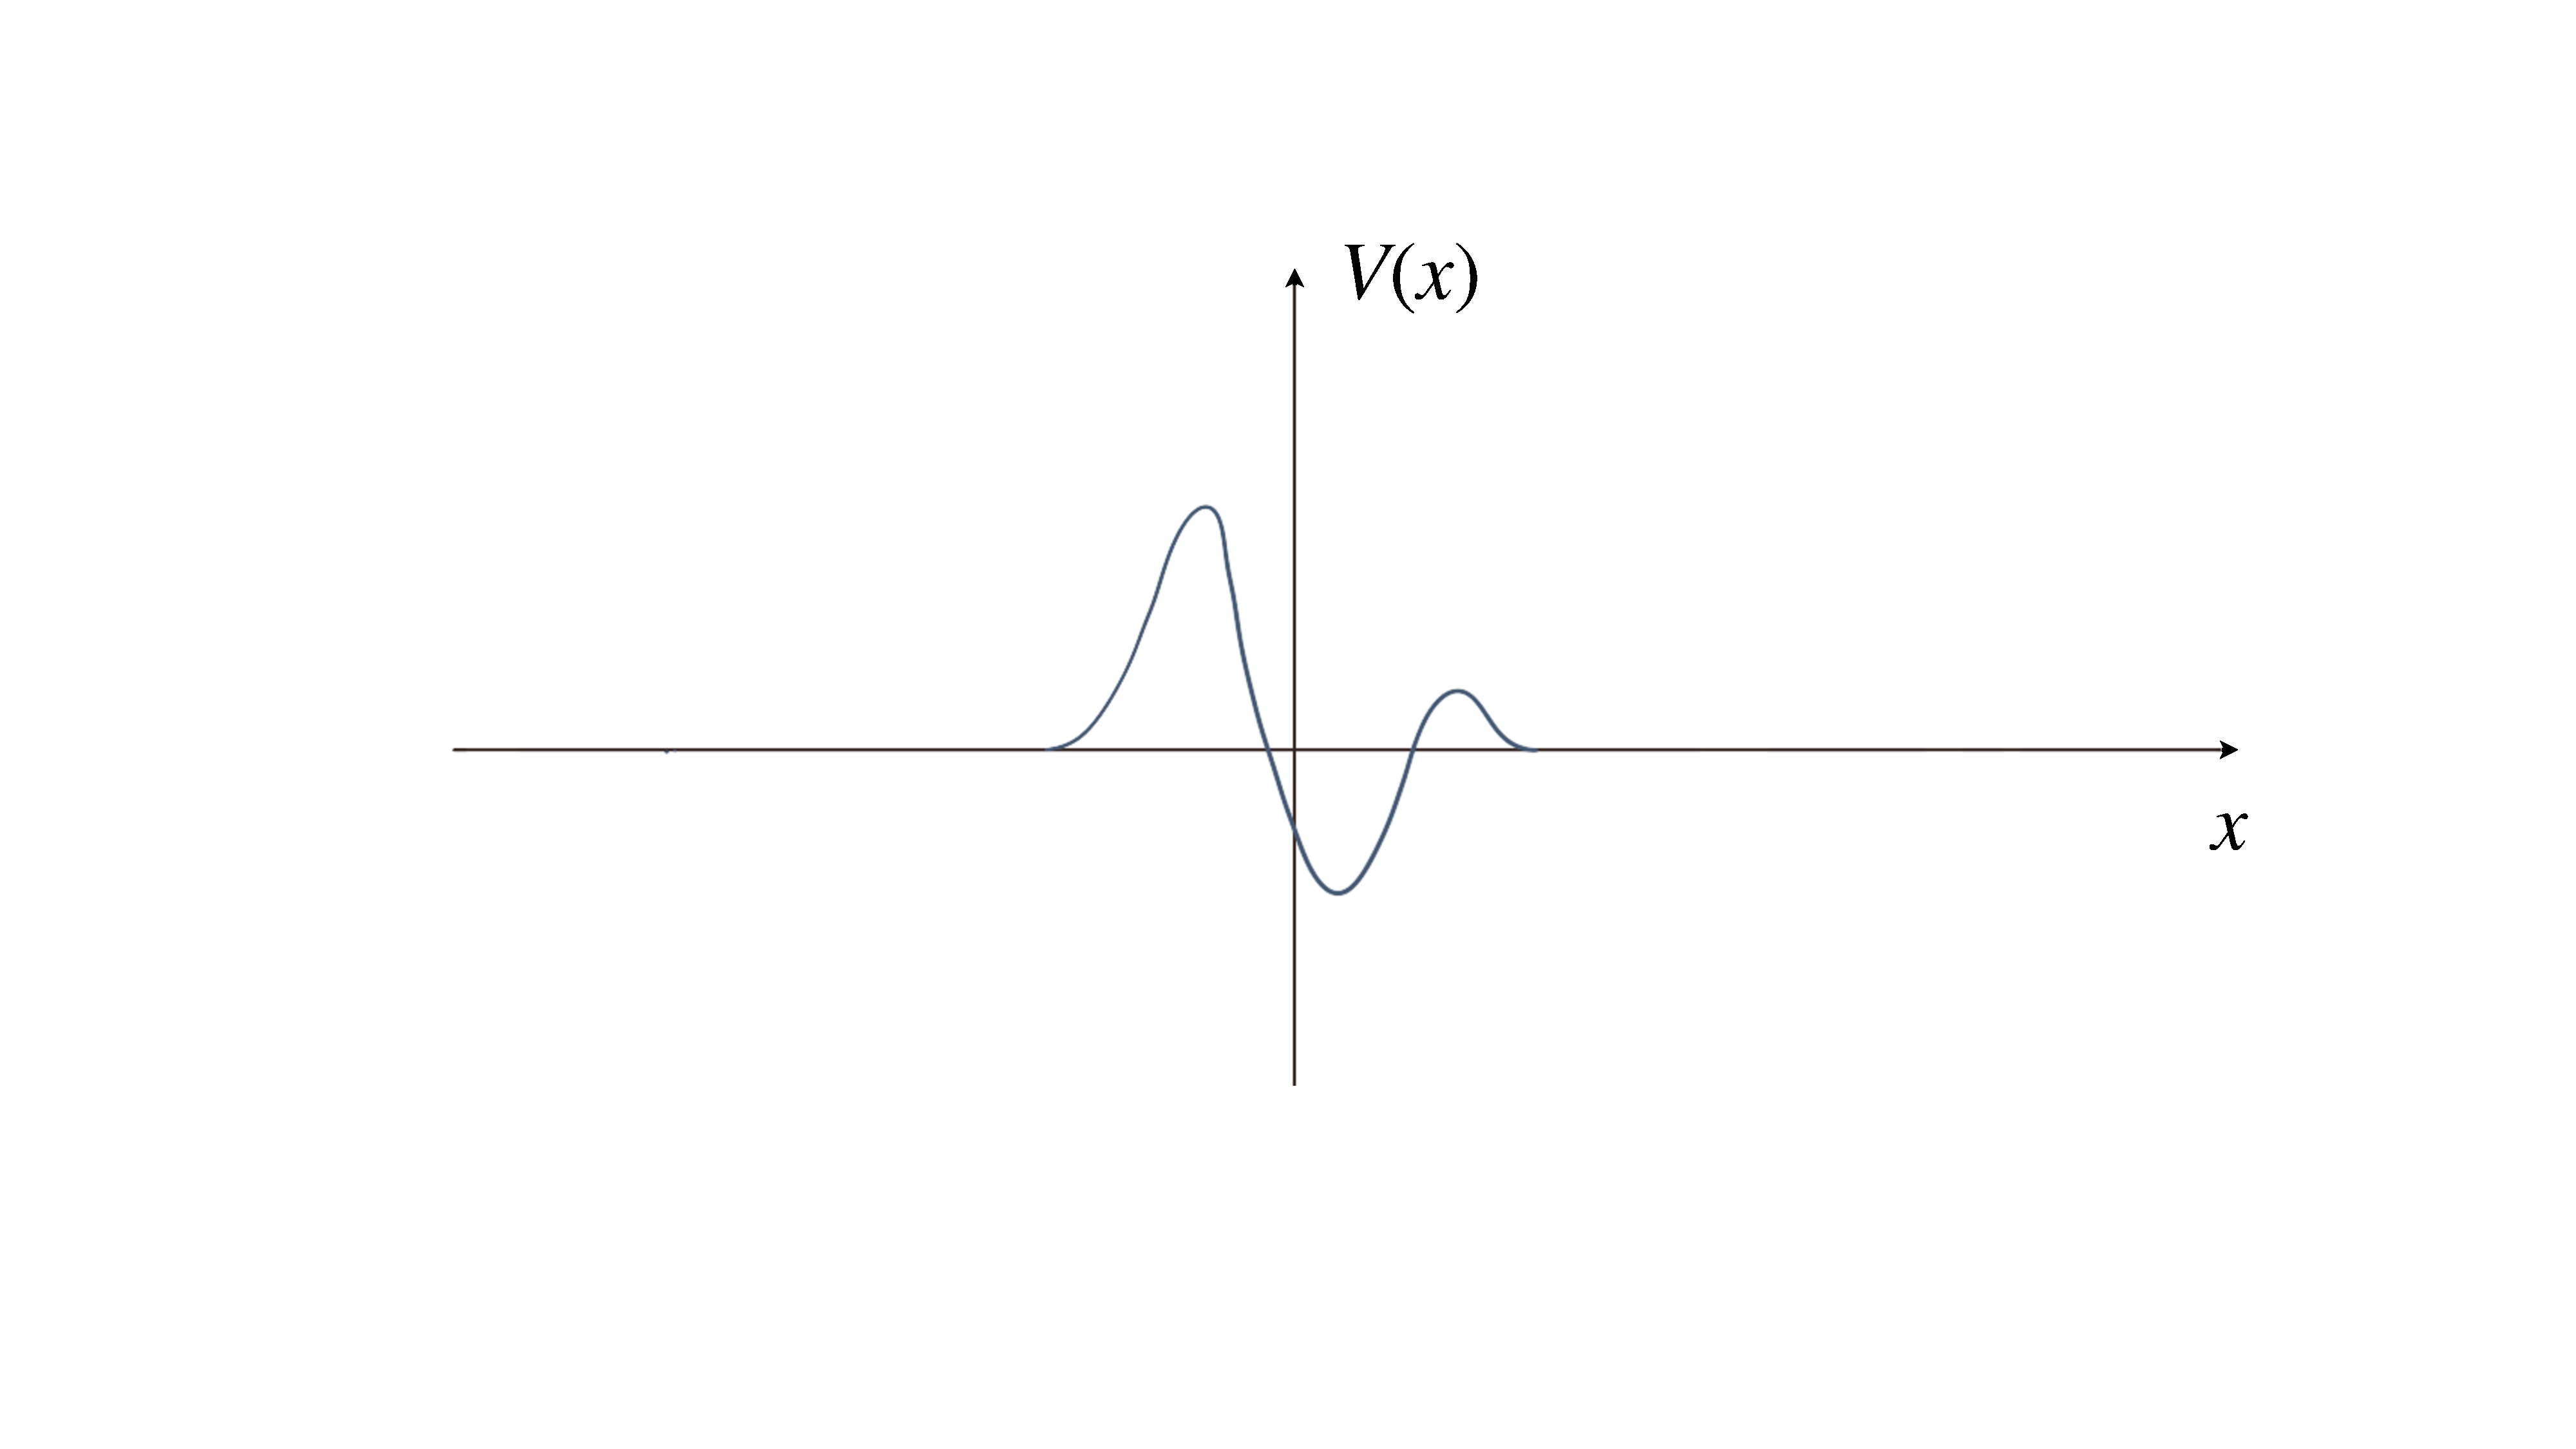
\includegraphics[width=0.7\textwidth]{Figures/Potential-1}
        \caption{Illustration of a one-dimensional potential which is vanishing at large values of $x$ far from the localized region where the potential is non-zero.}
        \label{fig:potential-1}
    \end{figure}


One can calculate the various probabilities of scattering by seeking solutions that are free particles at $x \rightarrow \pm \infty$: the resulting wave functions will be a combination of the two types of solutions (right-moving and left-moving). The problem is then posed in a stationary fashion, and we will look for solutions $\psi(x)$ of the form of a particle probing the potential from left to the right,
\begin{equation}
\psi_L(x) = \left \{ 
    \begin{matrix}
 e^{ikx} + r e^{-ikx}  \\
 t e^{ikx} 
\end{matrix}
    \right . \; \; \; \; 
    \begin{matrix}
 x \rightarrow -\infty  \\
 x \rightarrow +\infty 
\end{matrix}
\end{equation}
where $r$ and $t$ are complex numbers which will be referred to as {\it reflection} and {\it transmission} amplitudes. 

While the scattering process is inherently a time-dependent concept, here we are modeling the scattering by a system of plane waves. It could be thought of as a beam of particles thrown towards the potential from the left, with part of the beam being reflected and part being transmitted.

Taking the simple example of a plane wave for the free particle, for its interpretation in terms of number of particles and probabilities it is useful to compute the probability current,

\[ j = \frac{i\hslash}{2m} (\psi^* \frac{\partial \psi}{\partial x} -  \frac{\partial \psi^*}{\partial x} \psi.)\]

By simply replacing the wave function solutions in this equation yields on the left ($x \rightarrow -\infty$)
\begin{eqnarray*}
j & = & \frac{\hslash}{2im} [(e^{-ikx}+r^* e^{ikx})(ike^{ikx}-ikr e^{-ikx})-(e^{ikx}+r e^{-ikx})(-ike^{-ikx}+ikr^* e^{ikx})] \\
& = & \frac{\hslash k}{2m} [ 1 -r e^{-i2kx} + r^* e^{i2kx} -rr^* +1 - r^*e^{i2kx} + re^{-i2kx} - r r^*] \\
& = & \frac{\hslash k}{m} (1 - |r|^2 ).
\end{eqnarray*}
On the right instead ($x \rightarrow +\infty$) one gets
\[ j = \frac{\hslash}{2im} ik ( t^*t + t t^* ) = \frac{\hslash k}{m} |t|^2.\]
The conservation of the probability current yields
\[|r|^2 + |t|^2 = 1,\]
where $R = |r|^2$ and $T = |t|^2$ can be interpreted as the probabilities of reflection and transmission respectively, where on the left there is the sum of two fluxes of particles, one which is propagating towards the right with a flux of $T$ and velocity $+k/m$ and a flux of particles moving to the left with a flux $R$ with a velocity $-k/m$, while on the right side the transmitted particles for a beam of flux $T$ with a velocity $+k/m$. 

This is the so-called case of ``scattering from the left''. The same can be done for the case of the scattering from the right, where the problem is posed in the following terms (a beam of particles coming from the right):
\begin{equation}
\psi_R(x) = \left \{ 
    \begin{matrix}
 e^{-ikx} + r' e^{ikx}  \\
 t' e^{-ikx} 
\end{matrix}
    \right . \; \; \; \; 
    \begin{matrix}
 x \rightarrow +\infty  \\
 x \rightarrow -\infty 
\end{matrix}
\end{equation}

From this we can note that there is a simple ``mirror'' relation between the case of the scattering from the left and the scattering from the right. Since the potential $V(x)$ is real, then $\psi_L^*$ is also a solution of the Schr\"odinger equation, 
\[ -\dfrac{\hslash^2}{2m} \dfrac{\partial^2 \psi}{\partial x^2} = (E-V(x)) \psi, \]
in the form
\begin{equation}
\psi_L^*(x) = \left \{ 
    \begin{matrix}
 e^{-ikx} + r^* e^{ikx}  \\
 t^* e^{-ikx} 
\end{matrix}
    \right . \; \; \; \; 
    \begin{matrix}
 x \rightarrow -\infty  \\
 x \rightarrow +\infty 
\end{matrix}
\end{equation}

We then recognize that
\begin{equation}
\dfrac{\psi_L^*(x) -r^* \psi_L(x)}{t^*}  = \left \{ 
    \begin{matrix}
 (1-|r|^2) e^{-ikx} /t^* = |t|^2 e^{-ikx} / t^* = t e^{-ikx} \\
 t^* e^{-ikx} -r^* t e^{ikx} = e^{-ikx} -r^* \dfrac{t}{t^*} e^{ikx} 
\end{matrix}
    \right . \; \; \; \; 
    \begin{matrix}
 x \rightarrow -\infty  \\
 x \rightarrow +\infty 
\end{matrix}
\end{equation}

which is in the same form as the solution for the scattering from the right, if we take $t = t'$ and $r'= r \frac{t}{t^*}$. This is a very interesting result that shows that the transition amplitude is the same {\bf irrespective of the shape of the potential} and that the reflection only differs by a phase. The transmission and reflection probabilities $R$ and $T$ are thus the same in the scattering from the left and in the scattering from the right.

\subsection{Scattering in three dimensions and scattering amplitudes}
In the much more realistic case of a three dimensional potential localised in space, a similar stationary formalism can be applied. In this case the incoming beam of particles is represented by a plane wave, or a beam of particles with a given momentum and in the $z$ direction ($\psi(\vec{r}) = e^{ikz}$). The scattered particles will then be represented by a spherical wave with a given scattering amplitude which depends on the scattering direction $\psi(\vec{r}) =  f(\theta,\phi) \frac{e^{i\vec{k}.\vec{r}}}{r}$. The dependence in $1/r$ of the scattered wave function is obtained as a result of solving the Schr\"odinger equation and can be simply interpreted in terms of density of states as $|\psi|^2$ will be expanding over a sphere of surface proportional to $r^2$. The resulting overall wave function will then be  written as
\begin{equation}
\label{eq:scat-3d}
    \psi(\vec{r}) = e^{ikz} + f(\theta,\phi) \frac{e^{i\vec{k}.\vec{r}}}{r}.
\end{equation}
In this case the probability current can be expressed as
\[ \vec{j} = \frac{\hslash}{2im} (\psi^* \nabla \psi -  \psi \nabla \psi^*  ) \]
The current can also be separated into an incident current obtained from the incident ($e^{ikz}$) part of the wave function,
\[\vec{j}_{incident} =  \frac{\hslash k}{m} \hat{z},\]
which can be seen as a beam of particles with velocity $\hslash k/m$ along the $z$ direction. We will derive the scattered current in a given direction in space $(\theta,\phi)$ under the assumption that the potential is central (i.e. that it does not depend on $\phi$), and neglecting the $1/r^2$ terms from the derivative in terms of the polar angle $\theta$, which are suppressed as $1/(r \sin \theta) \partial f \partial \theta$ and the derivative of $1/r$. One gets\footnote{We started from \[ \nabla = \pd{}{r} \hat{r} + \frac{1}{r}\pd{}{\theta}\hat{\theta}+\frac{1}{r\sin\theta}\pd{}{\phi}\hat{\phi}.\]The derivative in $\phi$ in the last term will have no effect as the potential is central, and so we immediately see that \[\nabla\psi = \nabla\left(\frac{1}{r}f(\theta,\phi)e^{i\vec{k}\cdot\vec{r}}\right)= \pd{\psi}{r}\hat{r}+\mathcal{O}\left(\frac{1}{r^2}\right)\].}
\[\vec{j}_{scattered} \sim  \frac{\hslash k}{m} \frac{|f(\theta)|^2}{r^2}\hat{r} + \mathcal{O}\left(\frac{1}{r^3}\right)\]

If we then consider the flux of particles across an element area $dA$ in space, which spans a solid angle $d\Omega = dA/r^2$, then we have
\[\vec{j}_{scattered} \cdot \hat{r} \, dA =  \frac{\hslash k}{m} |f(\theta)|^2 d\Omega.\]
Taking the ratio of the scattered flux to the incident beam flux will thus give the differential cross section $d\sigma$,
\[ d\sigma = \frac{\vec{j}_{scattered}}{\vec{j}_{incident}} = \frac{\hslash k |f(\theta)|^2 /m d\Omega}{\hslash k /m}
 = |f(\theta)|^2 d\Omega, \]
while the differential cross section can then be expressed as
\[ \frac{d\sigma}{d\Omega} = |f(\theta)|^2 .\]We have therefore seen that the scattering amplitude and the differential cross section are linked together.
 
\subsection{Partial waves} \label{sec:partialwaves}
In a central potential, i.e. which does not depend on $\phi$, it is interesting to seek solutions of the Schr\"odinger equation (similarly to the resolution of the Hydrogen atom) in terms of spherical harmonics. We start from the fact that the Laplacian operator $\nabla^2$ can be written, in spherical coordinates\footnote{We have
\[ \vec{r}=\begin{cases}x = r \sin\theta \cos\phi\\ y = r \sin\theta \sin\phi\\ z = r \cos\theta\end{cases}\]
and the unit vectors are 
\[ \begin{cases}\hat{r}=\frac{d\vec{r}/dr}{|d\vec{r}/dr|} = \frac{(\sin\theta\cos\phi, \sin\theta\sin\phi,\cos\theta)}{\sqrt{(\sin\theta\cos\phi)^2+(\sin\theta\sin\phi)^2+(\cos\theta)^2}}=(\sin\theta\cos\phi,\sin\theta\sin\phi,\cos\theta)\\
\hat{\theta}=\frac{d\vec{r}/d\theta}{|d\vec{r}/d\theta|} = \frac{(r\cos\theta\cos\phi, r\cos\theta\sin\phi,-r\sin\theta)}{r}=(\cos\theta\cos\phi,\cos\theta\sin\phi,-\sin\theta)\\
\hat{\phi}=(-\sin\phi,\cos\phi,0)\\
\end{cases}\]
thus
\begin{align*}
    \pd{\hat{\theta}}{\phi} &= (-\cos\theta\sin\phi, \cos\theta\cos\phi, 0) = \cos\theta\hat{\phi},\\
    \pd{\hat{\phi}}{\theta}&=0,\\
    \pd{\hat{\phi}}{\phi}&=(-\cos\phi, -\sin\phi, 0).
\end{align*}
}, as
\begin{eqnarray*}
 \nabla^2 &=  \dfrac{1}{r^2} \dfrac{\partial}{\partial r} \left( r^2 \dfrac{\partial}{\partial r} \right) + \dfrac{1}{r^2 \sin \theta} \dfrac{\partial}{\partial \theta}  \left( \sin \theta \dfrac{\partial}{\partial \theta} \right) + \dfrac{1}{r^2 \sin^2 \theta}   \left( \dfrac{\partial^2}{\partial \phi}  \right) \\ 
    & =  \dfrac{1}{r^2} \dfrac{\partial}{\partial r} \left(r^2 \dfrac{\partial}{\partial r} \right) - \dfrac{\vec{L}^2}{\hslash^2 r^2},
\end{eqnarray*}
where we used the fact that the partial derivative in $\phi$ will have no effect, and that $\vec{L}^2 = (\vec{r} \times \vec{p})^2 = (\vec{r} \times  -i\hslash \nabla)^2$. With a bit of math (in which we simply took into account how the derivatives of the unit vectors are written, cf. footnotes), we get
\begin{equation}\label{eq:ellequadro}\vec{L}^2 = -\hslash^2\left [ \dfrac{\partial^2}{\partial \theta^2} + \dfrac{1}{\tan \theta} \dfrac{\partial}{\partial \theta} + \dfrac{1}{\sin^2 \theta}\dfrac{\partial^2}{\partial \phi^2}  \right ].\end{equation}
 
The  Schr\"odinger equation $E\psi=-\hslash^2/2m\nabla^2\psi+V\psi$ in a central potential  $V(r)$ can then be written as
\[ E \psi = -\frac{\hslash^2}{2m} \frac{1}{r^2} \frac{\partial}{\partial r} \left ( r^2 \frac{\partial}{\partial r} \right ) \psi  +  \frac{\vec{L}^2}{2 m r^2} \psi +V(r) \psi.\]
Similarly to the case of the hydrogen atom, we can solve this equation via separation of variables, by expressing the wave function as the product between a radial wave function $R(r)$ and an angular wave function $P_l(\theta)$ (given the assumption of a central potential and therefore no $\phi$ dependence). We obtain
\begin{eqnarray}
\label{eq:SchrodingerSpherical}
E\psi(r,\theta)=E R(r) P_l (\theta) = & -\dfrac{\hslash^2}{2m} P_l(\theta) \frac{1}{r^2} \dfrac{\partial}{\partial r} \left ( r^2 \dfrac{\partial}{\partial r} \right ) R(r) \nonumber \\  & +  R(r)\dfrac{\vec{L}^2}{2 m r^2} P_l(\theta) + V(r) R(r) P_l (\theta),
\end{eqnarray}
where the index $l$ was conveniently introduced as we already know that the angular part of the wave function will be solved with Legendre polynomials. Having restricted ourselves to $\phi$-independent solutions, the Schr\"odinger equation separates into two equations, an angular and a radial one. The angular part is
\[\vec{L}^2 P_l(\theta) = \hslash^2 l(l+1) P_l(\theta)\]
which can then be written in terms of $w = \cos \theta$ and therefore $ d w   = - \sin \theta d\theta$, from which one can write \(\partial f/\partial \theta=\partial f/\partial w\cdot \partial w/\partial \theta\) and get
\[ \dfrac{\partial f}{\partial \theta^2} = \dfrac{\partial }{\partial \theta} \left (  -\sin \theta \dfrac{\partial f}{\partial w} \right ) = - \cos \theta \dfrac{\partial f}{\partial w} + \sin^2 \theta \dfrac{\partial^2 f}{\partial w^2} = - w \dfrac{\partial f}{\partial w} + (1-w^2) \dfrac{\partial^2 f}{\partial w^2}.\]
One can then replace these expressions for the first and second order derivatives in $\theta$ in Eq. \eqref{eq:ellequadro} to write the angular equation as
\[  \boxed{ \dfrac{\partial}{\partial w} (1-w^2) \dfrac{\partial}{\partial w} P_l(w)  + l(l+1) P_l(w) =0 },\]
where we wrote with no loss of generality the eigenvalue of the \(\vec{L}^2\) operator as \(l(l+1)\).

In the separation of variables, using the constant $\hslash^2 l(l+1)$, from Eq.~\eqref{eq:SchrodingerSpherical} the radial equation will become:
\begin{eqnarray*}
[E -V(r)]  R(r) P_l(\cos \theta) & = & -\dfrac{\hslash^2}{2m} P_l(\cos \theta) \dfrac{1}{r^2} \dfrac{\partial}{\partial r} \left ( r^2 \dfrac{\partial}{\partial r} \right ) R(r) \\
& & + \dfrac{\hslash^2 l(l+1)}{2mr^2} R(r) P_l (\cos \theta), %+ V(r) R(r) P_l (\cos \theta)
\end{eqnarray*}
which reduces to
\[ [E -V(r)]  R(r) = -\frac{\hslash^2}{2mr^2}  \frac{1}{r^2} \frac{\partial}{\partial r} \left ( r^2 \frac{\partial}{\partial r} \right ) R(r) + \frac{\hslash^2 l(l+1)}{2mr^2} R(r).\]

If we take the expression of the (non-relativistic) kinetic energy, and define the normalised potential $\tilde{V}(r)$ as
\[ E = \dfrac{\hslash^2 k^2}{2m}  \; \; \; \; {\rm and} \; \; \; \; \tilde{V}(r) = \dfrac{2m}{\hslash^2} V(r), \]
then the radial part of the Schr\"odinger equation can be written as
\[\boxed{ \left [  \dfrac{\partial^2}{\partial r^2} + \dfrac{2}{r}  \dfrac{\partial}{\partial r} - \dfrac{l(l+1)}{r^2} - \tilde{V}(r) + k^2 \right ] R_l(r) = 0}.\]

As we had anticipated with the introduction of the index $l$, we can recognise  $P_l$ as the Legendre polynomials, which are eigenstates of the angular momentum operator $\vec{L}^2$ and thus solutions of the angular part of the Schr\"odinger equation.

The {\bf partial wave} expansion consists in writing a generic wave function as a linear combination of partial waves, each of which is a solution of the Schr\"odinger equation in the separation of variables:
\begin{equation}
    \psi = \sum_{l=0}^{\infty} R_l(r) P_l (\cos \theta)).
\end{equation}

In absence of a potential, the free particle system will correspond to $\tilde{V}(r) = 0$ and therefore the radial equation can be written as

\[\left [ \dfrac{\partial^2}{\partial r^2} - \dfrac{l(l+1)}{r^2} + k^2 \right ] (r R_l(r)) = 0.\]

The solutions to this equation are the {\it Bessel spherical functions} %(see Appendix~\ref{appendix:bessel}),
. It can be seen that for $l=0$ the solution is very simple,
\[R_0(r) = \dfrac{e^{\pm i kr}}{r},\]
i.e. ingoing (outgoing) a plane wave, depending on the sign $\pm$.

Again, when far away from the region where the potential is non-vanishing, we must  also seek for the plane wave solutions as the {\it incident} wave function
\[ \psi_{incident}(\vec{r}) = e^{i kr \cos \theta}  \]
Now, let's express the plane wave in terms of partial wave expansion, i.e. in the form
\begin{equation}\label{eq:eikappazeta}
  e^{ikz} = e^{ikr \cos \theta} = \sum_{l=0}^{\infty} R^p_l(r) P_l (\cos \theta).
\end{equation}
We can use the properties of Legendre polynomials, such as their orthogonality, which can be expressed in the integral form
\[\int_{-1}^{1} P_l(x)P_m(x) dx = \dfrac{2}{2l+1} \delta_{ml},\]
From this we can easily write $R^p_l(r)$ in a simple form. Let's multiply both terms of Eq. \eqref{eq:eikappazeta} by $P_m(\cos\theta)$, and integrate in $dw=d(cos\theta)$: we get
\[
\int_{-1}^1 dw P_m(w) e^{ikrw} =\int_{-1}^1\sum_{l=0}^\infty dw R_l^p(r)P_l(w) = \frac{2}{2m+1} R_m^p(r).
\]
Thus we have (we change label from $m$ to $l$)
\begin{eqnarray}
R^p_l(r) & = & \dfrac{2l+1}{2} \int_{-1}^1 dw P_l(w)e^{ikrw} \nonumber \\
%\sum_{m=0}^{\infty} R^p_m(r) \int_{-1}^{1}  P_m (w)P_l (w) dw) \nonumber \\
%& = & \dfrac{2l+1}{2} \sum_{m=0}^{\infty} R^p_m(r) \delta_{lm}) \nonumber \\
%& = &  \dfrac{2l+1}{2} \int_{-1}^{1} e^{ikr w} P_l(w) dw \nonumber  \\
& = & \dfrac{2l+1}{2} \left [ \dfrac{e^{ikr w} }{ikr}  P_l(w)  \right ]_{-1}^{1} - \dfrac{1}{ikr} \int_{-1}^{1} e^{ikr w} \dfrac{dP_l(w)}{dw}dw \nonumber  \\ 
&= & \dfrac{2l+1}{2} \dfrac{1}{ikr}  \left [  e^{ikr}-(-1)^l  e^{-ikr} \right ] + \mathcal{O}\left (\dfrac{1}{r^2} \right ),
 \end{eqnarray}
where we integrated by parts (and identified in this way the $\mathcal{O}(1/r^2)$ terms), and used the fact that $P_l(1)=1, P_l(-1)=(-1)^l$. Remember, we are looking at the wave function far away from the potential, i.e. for $r\to\infty$!
This is a very interesting result which shows that a plane wave can simply be decomposed in two spherical waves, one which is outgoing and the other ingoing:
\[ \boxed{ \psi_{incident}(\vec{r}) = \left ( \sum_{l=0}^{\infty}  \dfrac{2l+1}{2ik} P_l (\cos \theta) \right ) \dfrac{e^{ikr}}{r} - \left ( \sum_{l=0}^{\infty}  \dfrac{2l+1}{2ik} (-1)^l P_l (\cos \theta) \right ) \dfrac{e^{-ikr}}{r} .}\] 

Why is this important? Because with these simple expressions we can express the wave function in the form of Eq.~\eqref{eq:scat-3d} ($r\to\infty$). We first expand the scattering amplitude $f(\theta)$ (which, again, does not depend on $\phi$ as the potential is central) in terms of partial waves, as
\begin{equation}\label{eq:fthetaform} f(\theta) = \sum_{l=0}^{\infty}  \dfrac{2l+1}{k} f_l P_l(\cos \theta),\end{equation}
where we chose this form so that the coefficients of the expansion, $f_l$, have a clear correspondence with the previous equation. Note  that $f_l$ do not depend on $\theta$ but rather depend on $k$ (and on the chosen potential $V$).
We can then write the wave function for $r\to\infty$ by replacing the partial wave expansion of the plane wave in Eq.~\eqref{eq:scat-3d}: we get
\[\psi(\vec{r}) =  \sum_{l=0}^{\infty}  \dfrac{2l+1}{2ik} P_l (\cos \theta) \left ( (-1)^{l+1} \dfrac{e^{-ikr}}{r} +(1 + 2i f_l)  \dfrac{e^{ikr}}{r}  \right ) P_l (\cos \theta),\]
where the first term is ingoing and the second one is outgoing.

It is interesting to note that, in this spherically symmetric case, the total wave function decomposes in different values of $l$ because the angular momentum is conserved. For each individual value of $l$, the scattering system is completely equivalent to the 1D case: the notion of scattering from the left and from the right  applies nicely also in the case of an incoming and outgoing spherical wave. In the case of a symmetrical potential one has $r'= r$, which implies that the equation derived in the 1D case  $r'= r^*\frac{t}{t^*}$ leads to
\begin{equation}
\label{eq:symmetricalpotential}
rt^* + r^*t = 0.
\end{equation}
We can imagine the scattering of an incoming spherical wave in one dimension as a simultaneously left-moving and right-moving incoming wave and the outgoing wave, which when $x \rightarrow -\infty$ results in the initial beam of particles and the reflected one $e^{ikx}+r e^{-ikx}$ -- to which one should add the particles transmitted from the right, i.e. $t e^{-ikax}$. Given that the conservation of the probability current (i.e. of the number of particles) yielded $R + T = 1 $, by using Eq.~\ref{eq:symmetricalpotential} one can see that $|r+t|^2 = 1$ also in this context\footnote{There is much more to this in the theory of the Scattering matrix which is beyond the scope of these lectures.}. 

In the context of the spherical 3D scattering, this means that $|(1 + 2i f_l)|^2 = 1$, i.e. one can write $(1 + 2i f_l) = e^{i2\delta_l(k)}$, where we highlighted the dependence on $k$. In other words, we can write the scattering amplitudes (Eq. \eqref{eq:fthetaform})  as a function of the {\bf phase shifts} $\delta_l(k)$ only,
\begin{equation}
\label{eq:scatteringamplitude}
f(\theta) = \dfrac{1}{2ik} \sum_{l = 0}^{\infty} (2l+1) (e^{i2\delta_l(k)} - 1) P_l(\cos \theta) 
\end{equation}

Then, following what we said in the previous section, from the scattering amplitude one gets the differential scattering cross section as a function of the scattering angle $\theta$,
\[ \dfrac{d\sigma}{d \Omega} = |f(\theta)|^2 = \dfrac{1}{k^2} \sum_{l, l'} (2l+1)(2l'+ 1) f_l f_{l'}^* P_l(\cos \theta)P_{l'}(\cos \theta) .\]
In order to compute the total cross section, we can use the orthogonality of the Legendre polynomials to get
\begin{equation}
\label{eq:TotXS}
\sigma = \int d\Omega \od{\sigma}{\omega} = 2\pi \int_{-1}^{1} \dfrac{d\sigma}{d \Omega} d\cos \theta = \dfrac{4\pi}{k^2} \sum_l (2l + 1) \sin^2 \delta_l(k) 
\end{equation}

Since $P_l(1) = 1$, the expression of $f(0)$ from Eq.~\eqref{eq:scatteringamplitude} is
\[ f(0) = \dfrac{1}{2ik} \sum_{l = 0}^{\infty} (2l+1) (e^{i2\delta_l(k)} - 1)= \sum_{l = 0}^{\infty} \dfrac{2l+1}{k} e^{i\delta_l(k)} \sin \delta_l(k).\]
This results in the following relation, known as the {\bf optical theorem}:
\begin{equation}
\boxed{ \sigma = \dfrac{4\pi}{k} \Im \, f(0),}
\end{equation}
which relates the forward cross section at $\theta = 0$ with the total scattering cross section. This result can be intuitively memorized as the conservation of probability  or the conservation of total number of particles, whereby the decrease in number of particles that are unaltered by the scattering should equal the ones which are scattered in any direction.

The time independent formalism, though very powerful and yielding deep and consequential results, is intrinsically not fully satisfactory when it comes to describing transient effects. For this purpose the time dependent perturbations is more appropriate and more general. However, the stationary formalism will be used for several calculations in nuclear physics. 

\vspace{0.5cm}

{\bf Important note} from the expression of the total cross section of Eq.~\ref{eq:TotXS} one can infer that the total cross section is necessarily bounded by:

\begin{equation}
\label{eq:TotXS2}
\sigma < \dfrac{4\pi}{k^2} \sum_l (2l + 1) 
\end{equation}

One should also note that the angular momentum of the particle will be given by $L = \vec{p} \wedge \vec{r}$ where then $l \hslash = \hslash k r \sin \theta$, where $r \sin \theta$ is a constant -- the impact parameter $b$ of the scattering reaction. So for a given momentum of the particle $p = \hslash k$, the number of partial waves to consider will be limited by the range $R
^{max}$ of the interaction: for example, in the case of the Rutherford scattering this was due to the fact that outside the atom the Coulomb repulsion is screened by the atomic electrons, or in the case of nuclear interactions which, as we will see, are short-ranged. It should also be noted that the number of partial waves to consider increases with the energy of the particle $n = k R^{max}$: in fact, the cross section is bounded by
\begin{eqnarray}
\label{eq:TotXS3}
\sigma & < & \dfrac{4\pi}{k^2} \sum_{l=0}^n (2l + 1) \nonumber \\
\sigma  & < & \dfrac{4\pi}{k^2} (n+1)^2 \nonumber \\
\sigma  & < & \dfrac{4\pi}{k^2} (kR^{max} + 1)^2 \nonumber \\
\sigma  & < & 4 \pi \left(R^{max} + \dfrac{1}{k}\right)^2 = 4 \pi (R^{max} + \lambda)^2,
\end{eqnarray}
where $\lambda = 1/k$ is the corresponding wavelength of the particle.


%%%%%%%%%%%%%%%%%%%%%% Time dependent perturbations
\section{Time dependent perturbation theory}
In order to be able to describe a particle physics experiment -- e.g. the interaction of a particle with a potential, the decay of a particle, the cross-section of an interaction... -- we need to be able to calculate the probability of transition between the initial and final state of a quantum system. The idea is to do so by starting from the expansion which is performed for the time-dependent perturbation theory (summarised in the previous sections). For unbound states (as it is in the case of a scattering) there are infinite solutions to the Schr\"odinger equation with energy $E$ (i.e. the free-particle Schr\"odinger equation). We will use this basis to express the solution to the general Schr\"odinger equation (i.e. the one with the addition of a potential $V$), as a linear combination of its elements. The challenge comes from the fact that we will assume that $V$ is not only a function of position, but also of time ($V=V(\Vec{x},t)$). Let's see how we can address it.

We will call $H_0$ the hamiltonian of a free particle, and try to describe its interaction with a potential $V(\Vec{x},t)$. The possible quantum states of the particle will be the solutions $\psi$ to the  Schr\"odinger equation
\begin{equation}
\left[ H_{0} + V(\Vec{x},t) \right] \psi = i\hslash\frac{\partial\psi}{\partial t}.
\label{quantum-scattering:eq1}
\end{equation}
In general, this equation cannot be solved in a straightforward way: one needs to use perturbation theory in order to obtain an approximation of the solution. That's why we choose to use the base of the eigenfunctions $\Phi$ of the free-particle hamiltonian $H_0$, i.e.
\begin{equation*}
H_{0} = -\frac{\hslash^2}{2m}\nabla^{2}.
\end{equation*}
The eigenfunctions $\Phi$ are those which solve the equation
\begin{equation*}
H_{0}\Phi_{k}(\Vec{x},t) = E_{k}\Phi_{k}(\Vec{x},t),
\end{equation*}
and are labeled with the subscript $k$.
The normalisation of these wave functions is chosen such that we have $1$ particle per unit of volume $V$: orthonormality is then written as
\begin{equation*}
\int_{V}\Phi_{m}^{*}\Phi_{n}\;d^3\Vec{x} = \delta_{mn}.
\end{equation*}

In order to simplify notation, let's assume from now on that $\hslash=1$.
We are looking for a solution of Eq. \eqref{quantum-scattering:eq1} expressed in this basis, assuming that both the initial and final states (i.e. ``before'' and ``after'' the scattering process) are well-modeled by the hamiltonian of a free particle. This assumption means we are considering the potential as negligible for $t=0$ and $t=\infty$.
We write the solutions of Eq. \eqref{quantum-scattering:eq1} as
\begin{equation*}
\psi(\Vec{x},t) = \sum_{k}a_{k}(t)\Phi_{k}(\Vec{x},t),
\end{equation*}
where we call $a_{k}(t)$ the (time-dependent!) coefficients of the expansion of $\Psi$ on the basis
\begin{equation}
\Phi_{k}(\Vec{x},t) = \Phi_{k}(\Vec{x})e^{-iE_{k}t}.\label{eq:freeparticlesol}
\end{equation}
The task is then to calculate an approximated expression for the coefficients $a(t)$.

Applying this general solution to the right-hand side of Eq. \eqref{quantum-scattering:eq1}, we obtain
\begin{equation*}
\begin{split}
i\frac{\partial\psi}{\partial t} & = \sum_{k}\left[ i\frac{\partial}{\partial t} (a_{k}(t)\Phi_{k}(\Vec{x})e^{-iE_{k}t})\right] = \\
& = \sum_{k}\left[i\frac{\partial a_{k}(t)}{\partial t} \Phi_{k}(\Vec{x})e^{-iE_{k}t} + a_{k}(t)\Phi_{k}(\Vec{x})E_{k}e^{-iE_{k}t} \right] = \\
& = \sum_{k} i \frac{\partial a_{k}(t)}{\partial t}\Phi_{k}(\Vec{x})e^{-iE_{k}t} + \sum_{k}a_{k}(t)\Phi_{k}(\Vec{x})E_{k}e^{-iE_{k}t}.
\end{split}
\end{equation*}
The left-hand side of Eq. \eqref{quantum-scattering:eq1} instead becomes
\begin{equation*}
\left[ H_{0} + V(\Vec{x},t) \right] \psi = \sum\left[ H_{0} + V(\Vec{x},t) \right] a_{k}(t) \Phi_{k}(\Vec{x})e^{-iE_{k}t},
\end{equation*}
to which we can apply Eq. \eqref{eq:freeparticlesol} and obtain
\begin{equation*}
\left[ H_{0} + V(\Vec{x},t) \right] \psi = \sum_{k} E_{k} a_{k}(t)\Phi_{k}(\Vec{x})e^{-iE_{k}t} + \sum_{k} V(\Vec{x},t)a_{k}(t)\Phi_{k}(\Vec{x})e^{-iE_{k}t}.
\end{equation*}
We can then simplify the two terms and write Eq. \eqref{quantum-scattering:eq1} as
\begin{equation}
\sum_{k} i\frac{\partial a_{k}(t)}{\partial t} \Phi_{k}(\Vec{x})e^{-iE_{k}t} = \sum_{k} V(\Vec{x},t)a_{k}(t)\Phi_{k}(\Vec{x})e^{-iE_{k}t}.
\label{quantum-scattering:eq2}
\end{equation}

As we said above, our assumption is that the particle is free in the initial and final state. This means that we can write its final state as one of the eigenstates of the free-particle hamiltonian $H_0$, the one with the label $f$:
\begin{equation*}
    |f\rangle = \Phi_{f}e^{-iE_{f}t}.
\end{equation*}
If we then multiply Eq. \eqref{quantum-scattering:eq2} by $\langle f|= \Phi_{f}^*e^{+iE_{f}t}$, we obtain
\begin{equation*}
\sum_{k} i\frac{\partial a_{k}(t)}{\partial t} \Phi_{f}^*(\Vec{x})\Phi_{k}(\Vec{x})e^{-i(E_{k}-E_{f})t} = \sum_{k}a_{k}(t) \Phi_{f}^*(\Vec{x})V(\Vec{x},t)\Phi_{k}(\Vec{x})e^{-i(E_{k}-E_{f})t}.
\end{equation*}

In the case of a time-independent potential, $V(\Vec{x},t) = V(\Vec{x})$, if we integrate over the volume $V$ we have
\begin{equation}\label{eq:idadt}
    i\frac{\partial a_{t}(t)}{\partial t} = \sum_{k} a_k(t) \int_{V} \Phi_{f}^*(\Vec{x})V(\Vec{x})\Phi_{k}(\Vec{x})\,d^3x\,\times e^{i(E_{k}-E_{f})t},
\end{equation}
where the integral is nothing else than
\begin{equation*}
\int_{V}\Phi_{f}^*(\Vec{x})V(\Vec{x})\Phi_{k}(\Vec{x})dV = \langle \Phi_{f}|V(\Vec{x})|\Phi_{k}\rangle.
\end{equation*}

As done for the final state, we can write the initial state as $|i\rangle = \Phi_{i}(\Vec{x},t)$, which means that $a_{k}(0) = \delta_{ik}$. We can then consider a weak perturbative potential which does not alter much the state of the particle: this means that the coefficient associated to the eigenstate $i$ of the free-particle hamiltonian will always be close to $1$, i.e.
\begin{equation*}
    a_{i}(t) \sim 1\,\,\,\, \forall t,
\end{equation*}
and that the coefficients associated to the other eigenstates will be almost zero, i.e.
\begin{equation*}
    a_{k\neq i}(t) \sim 0\,\,\,\, \forall t.
\end{equation*}
Under these assumptions, we can obtain the coefficient associated to the final state $f$, by replacing the expressions for $a_i(t)$ and $a_{k\neq i}(t)$ in Eq. \eqref{eq:idadt}: we get
\begin{equation*}
    \frac{\partial a_{f}(t)}{\partial t} = -i\int d^3x\;\Phi_{f}^*(\Vec{x})V(\Vec{x})\Phi_{i}(\Vec{x}) \times e^{i(E_{f}-E_{i})t},
\end{equation*}
which depends on the \emph{transition matrix}
\begin{equation*}
    T_{fi} = \int_{V}\Phi_{f}^*(\Vec{x})V(\Vec{x})\Phi_{i}(\Vec{x})\;d^3x.
\end{equation*}
The coefficient $a_f(t)$ at any time $T$ is then obtained by integrating between $t=0$ and $t=T$,
\begin{equation*}
    a_{f}(T) = -i\int_{0}^{T}T_{fi}e^{i(E_{f}-E_{i})t}\;dt,
\end{equation*}
Remember -- we assumed that the potential is independent on time, i.e. $V=V(\Vec{x})$. We can therefore move the transition matrix outside of the integration sign, obtaining
\begin{equation}
      a_{f}(T) = -iT_{fi}\int_{0}^{T}e^{i(E_{f}-E_{i})t}\;dt.
      \label{quantum-scattering:eq3}
\end{equation}
Eq. \eqref{quantum-scattering:eq3} shows that it is possible to introduce a transition between the state $|i\rangle$ and the state $|f\rangle$ with an amplitude $a_{f}(T)$.

In the end, we are studying a scattering experiment, so we are interested in knowing how probable the transition between the initial and the final state is. The probability to find the system in the final state $a_{f}(T)$ is $|a_{f}a^*_{f}|$, i.e.
\begin{equation*}
    P_{fi} = a_{f}(T)a_{f}^*(T) = |T_{fi}|^2\int_{0}^{T}\int_{0}^{T}e^{i(E_f-E_i)t}\times e^{-i(E_{f}-E_i)t'}dtdt'.
\end{equation*}
We usually deal with decaying particles or colliding particles, so it is convenient to ask ourselves what is the probability of transition between the initial and final state after some time $T$ has elapsed. We therefore define the \emph{transition rate} as
\begin{equation}
    \Gamma_{fi} = \frac{P_{fi}}{T}.
\end{equation}
In order to calculate this quantity, we start by performing the change of variables
\begin{equation}
    t\rightarrow t+\frac{T}{2},\;\;\;\;\; t' \rightarrow t' + \frac{T}{2},
\end{equation}
from which we can write
\begin{equation*}
    \Gamma_{fi} = |T_{fi}|^2\frac{1}{T}\int_{-\frac{T}{2}}^{\frac{T}{2}}\int_{-\frac{T}{2}}^{\frac{T}{2}} e^{i(E_{f}-E_{i})t}e^{-i(E_{f}-E_{i})t'}dtdt'.
\end{equation*}
This integral can be solved by separation of variables: we have
\begin{equation*}
    \int_{-\frac{T}{2}}^{\frac{T}{2}}e^{i(E_{f}-E_{i})t}dt = \frac{e^{i(E_{f}-E_{i})\frac{T}{2}}-e^{-i(E_{f}-E_{i})\frac{T}{2}}}{(E_{f}-E_{i})i},
\end{equation*}
and calling the difference\footnote{Keep in mind we put $\hslash=1$.} between the energy of the two states $E_{f} - E_{i} = \nu_{fi}$, we find
\begin{equation*}
     \int_{-\frac{T}{2}}^{\frac{T}{2}}e^{i(E_{f}-E_{i})t}dt = 2\frac{\sin{\nu_{fi}\frac{T}{2}}}{\nu_{fi}}.
\end{equation*}
We can repeat the reasoning with the integration over $t'$, and finally obtain 
\begin{equation*}
    \Gamma_{fi} = |T_{fi}|^2 \frac{4}{T}\frac{(\sin{\nu_{fi}\frac{T}{2}})^2}{\nu_{fi}^2}.
\end{equation*}
This relation shows that the transition rate drops quickly for high values of $\nu_{fi}$, i.e. for $E_f$ significantly different from $E_i$. Fig. \ref{fig:quantum-scattering:1} shows the evolution of
\begin{equation}\label{eq:sinusoidalenufi}
    \frac{4}{T}\frac{(\sin{(\nu_{fi}\frac{T}{2})})^2}{\nu_{fi}^2},
\end{equation}
as as a function of $\nu_{fi}$. We can see that in the limit $T\rightarrow\infty$, i.e. after the potential has had enough time to act on our particle, this function becomes a Dirac delta. This basically corresponds to imposing the conservation of energy in the scattering process.

\begin{figure}
%    \centering
    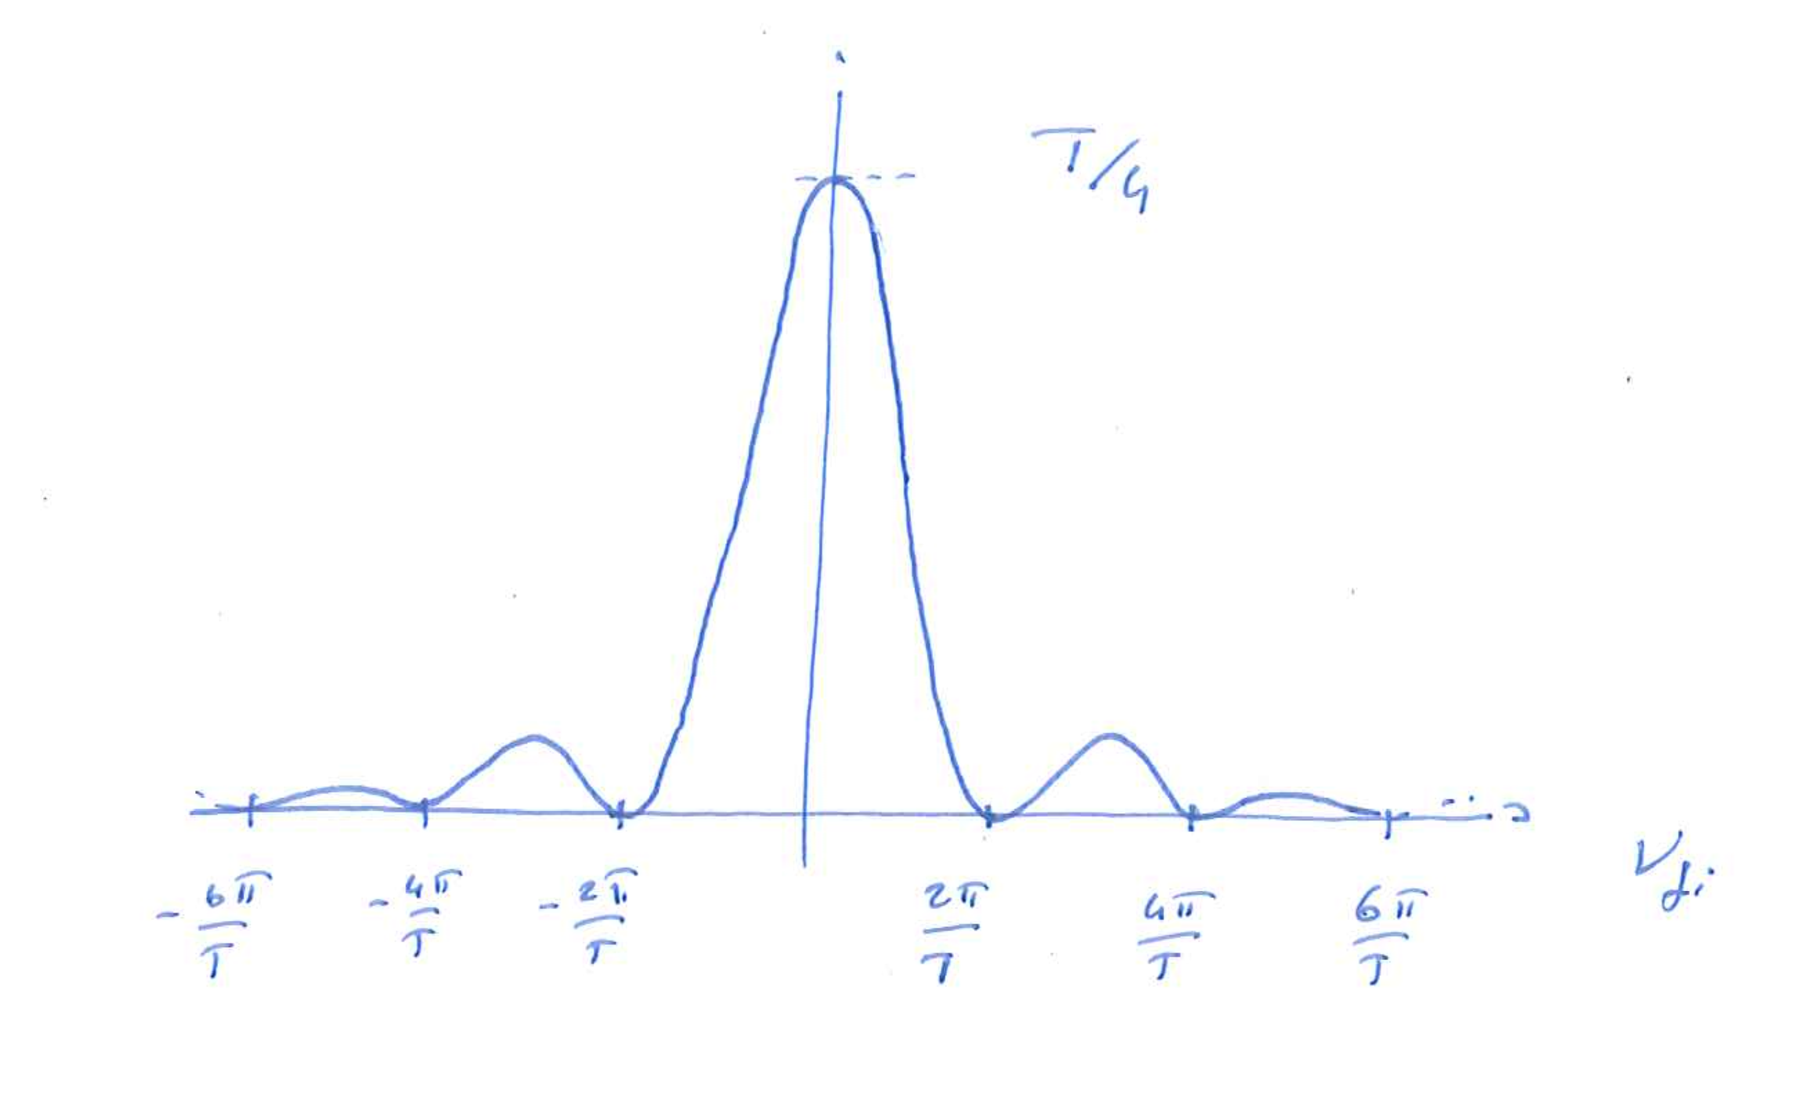
\includegraphics[scale=0.2]{Figures/qscat1.pdf}
    \caption{Evolution of Eq. \eqref{eq:sinusoidalenufi} as a function of the difference between the final and initial state energy $\nu_{fi}$.}
    \label{fig:quantum-scattering:1}
\end{figure}

Let's extend our reasoning to the continuum case, i.e. let's assume that we have a continuum of possible energy states, and that we are interested in the $dn$ accessible states in the range $[E_{f},E_{f}+dE_{f}]$. The total transition rate  can be expressed as a sum of continuous elements $d\Gamma_{fi}$ of transition rates, where
\begin{equation*}
    d\Gamma_{fi} = |T_{fi}|^2\times\frac{1}{T}\int_{-\frac{T}{2}}^{\frac{T}{2}}\int_{-\frac{T}{2}}^{\frac{T}{2}}e^{i(E_{f}-E_{i})t}e^{-i(E_{f}-E_{i})t'}dtdt'dn.
\end{equation*}
Considering long time intervals, $T\rightarrow\infty$, we have
\begin{equation*}
    d\Gamma_{fi} = |T_{fi}|^2\times\lim_{T\rightarrow \infty}\frac{1}{T}\int_{-\frac{T}{2}}^{\frac{T}{2}}\int_{-\frac{T}{2}}^{\frac{T}{2}}e^{i(E_{f}-E_{i})t}e^{-i(E_{f}-E_{i})t'}dtdt'dn.
\end{equation*}
In order to calculate the total rate, we can exploit the fact that the Fourier transform of $1$ is the Dirac delta function, $\delta$,
\begin{equation*}
    \int_{-\infty}^{+\infty}e^{ik(x-x_0)}dk = 2\pi\delta(x-x_0).
\end{equation*}
Therefore we have 
\begin{equation*}
    \int_{-\infty}^{+\infty}e^{i(E_{f}-E_{i})t'}dt' = 2\pi\delta(E_{f}-E_{i}),
\end{equation*}
and we can write the contribution to the total transition rate due to the several accessible states in the $[E_{f},E_{f}+dE_{f}]$ energy range as
\begin{equation*}
    d\Gamma_{fi} = |T_{fi}|^2 dn \lim_{T\rightarrow \infty}\left[\frac{1}{T}\int_{-\frac{T}{2}}^{\frac{T}{2}}e^{i(E_{f}-E_{i})t}dt \right] \times 2\pi\delta(E_{f}-E_{i}),
\end{equation*}
and so the total transition rate can be expressed as
\begin{equation*}
    \Gamma_{fi} = \int d\Gamma_{fi} = \int |T_{fi}|^2 \frac{dn}{dE_{f}}\lim_{T\rightarrow \infty}\left[\frac{1}{T}\int_{-\frac{T}{2}}^{\frac{T}{2}}e^{i(E_{f}-E_{i})t}dt\right]2\pi\delta(E_{f}-E_{i})dE_{f},
\end{equation*}
obtaining, using the delta properties on the integral,
\begin{equation*}
    \Gamma_{fi} = 2\pi\int|T_{fi}|^2 \frac{dn}{dE_{f}}\delta(E_{f}-E_{i})dE_{f}\times \lim_{T\rightarrow \infty} \frac{1}{T}\int_{-\frac{T}{2}}^{\frac{T}{2}}dt.
\end{equation*}

But
\begin{equation*}
    \lim_{T\rightarrow \infty} \frac{1}{T}\int_{-\frac{T}{2}}^{\frac{T}{2}}dt = 1,
\end{equation*}
therefore the total transition rate is written as
\begin{equation*}
    \Gamma_{fi} = 2\pi|T_{fi}|^2\left|\frac{dn}{dE_{f}}\right|_{Ei},
\end{equation*}
where
\begin{equation*}
      \left|\frac{dn}{dE_f} \right|_{E_{i}} = \rho(E_i)
\end{equation*}
is the density of accessible states in the final state, given the initial energy $E_{i}$. We can therefore write the total transition rate as
\begin{equation*}
    \Gamma_{fi} = 2\pi|T_{fi}|^2\rho(E_{i}).
\end{equation*}
For completeness, we report also its expression when $\hslash\neq1$:
\begin{equation*}
    \Gamma_{fi} = \frac{2\pi}{\hslash}|T_{fi}|^2\rho(E_{i}).
\end{equation*}

\section{Fermi's golden rule}
Until now assumed $a_{k\neq i} (t) \sim 0$: what happens if we relax this assumption? Let's take again Eq. \eqref{quantum-scattering:eq2} and keep only the assumption that $a_{i}(t) \sim 1$, and that $V=V(x)$: we have
\begin{equation*}
    i \sum_{k} \frac{\partial a_{k}(t)}{\partial t} \Phi_{k}(\Vec{x})e^{-iE_{k}t} = V(\Vec{x})\Phi_{i}(\Vec{x})e^{-iE_{i}t} + \sum_{k\neq i}  V(\Vec{x})a_{k}(t)\Phi_{k}(\Vec{x})e^{-iE_{k}t}.
\end{equation*}
Multiplying by $\langle f |$ and integrating over the volume $V$, we get
\begin{equation}
\begin{split}
    i\frac{\partial a_{f}(t)}{\partial t} &= \int_{V}d^3x\,\Phi_{f}^*(\Vec{x})V(\Vec{x})\Phi_{i}(\Vec{x})e^{i(E_{f}-E_{i})t} \\&+ \sum_{k\neq i}\int_V d^3x\Phi_f^*(\Vec{x})V(\Vec{x})a_{k}(t)\Phi_{k}(\Vec{x}) e^{i(E_{f}-E_{k})t}.
\end{split}
    \label{quantum-scattering:eq4}
\end{equation}

The strategy to get the solutions to the Schr\"odinger equation in this more general case ($a_{k\neq i} (t) \neq 0$) is to approximate $a_k(t)$ with the solutions from Eq. \eqref{quantum-scattering:eq3} (which were obtained assuming, at the first order, $a_{k\neq i}(t)=0)$: in other words, we write
\begin{equation*}
\begin{split}
    a_{k}(t) &= -i \int_{0}^{T}\left[\int_{V}\Phi_{k}^*(\Vec{x}) V(\Vec{x})\Phi_{i}(\Vec{x})d^3x \right] e^{i(E_{k}-E_{i})t'}dt'\\
    &= -i\frac{e^{i(E_k-E_i)t}}{i(E_k-E_i)}\int_V\Phi_k^*(\Vec{x}) V(\Vec{x})\Phi_i(\vec{x}) d^3x\\
    &= -\frac{e^{i(E_k-E_i)t}}{E_k-E_i} \int_V \Phi_k^*(\Vec{x}) V(\Vec{x})\Phi_i(\vec{x}) d^3x.
\end{split}
\end{equation*}
We then insert this expression in Eq. \eqref{quantum-scattering:eq4}, obtaining 
\begin{equation*}
\begin{split}
    \frac{\partial a_{f}(t)}{\partial t} &= \left[-i\int_{V} d^3x \Phi_{f}^*(\Vec{x}) V(\Vec{x})\Phi_{i}(\Vec{x}) \right] e^{i(E_{f}-E_{i})t} \\
    &+ (-i)(-1) \sum_{k\neq i} \frac{\int_{V}d^3x\Phi_{f}^*(\Vec{x})V(\Vec{x})\Phi_{k}(\Vec{x})\int d^3x\Phi_{k}^*(\Vec{x})V(\Vec{x})\Phi_{i}(\Vec{x})}{(E_{k}-E_{i})} e^{i(E_{k}-E_{i})t} e^{i(E_{f}-E_{k})t}.
\end{split}
\end{equation*}
%since
%\begin{equation*}
 %   a_{k}(t) = -i \int_{V}d^3x \Phi_{k}^*(\Vec{x}) V(\Vec{x}) \Phi_{i}(\Vec{x}) d^3x %\frac{e^{i(E_{k}-E_{i})t}}{i(E_{k}-E_{i})},
%\end{equation*}
%which is, integrating over the time $t'$, the solution at the first order for $a_{k}(t)$.

Using the bra-ket notation,
\begin{equation*}
    \langle f | V | i \rangle = \int_{V}\Phi_{f}^*(\Vec{x})V(\Vec{x})\Phi_{i}(\Vec{x}) d^3x,
\end{equation*}
we can write
\begin{equation*}
    \frac{\partial a_{f}(t)}{\partial t} = -i \left[\langle f | V | i \rangle + \sum_{k\neq i} \frac{\langle f | V | k \rangle\langle k | V | i \rangle}{E_{i}-E_{k}} \right] \times e^{i(E_{f}-E_{i})t}.
\end{equation*}

What we did is effectively to obtain a better approximation of the transition matrix element $T_{fi}$,
\begin{equation*}
    T_{fi} = \langle f|V|i\rangle + \sum_{k\neq i}\frac{\langle f |V|k\rangle\langle k |V|i\rangle}{E_{i}-E_{k}},
\end{equation*}
which is again a time-independent expression. We can insert it in Eq. \eqref{quantum-scattering:eq3}, 
and use this second-order evaluation of $T_{fi}$ in the expression of the Fermi's golden rule. The procedure can be iterated, obtaining more and more precise approximations of the solutions of the Schr\"odinger equation for an arbitrary potential.

\section{Perturbative calculation and particles exchange}\label{sec:perturbativecalc}
This iterative calculation has a fundamental interpretation in particle physics.
We have seen that at second order one has
\begin{equation}\label{eq:reminderTfi}
    T_{fi} = \langle f |V| i\rangle + \sum_{k\neq i}\frac{\langle f|V|k\rangle\langle k |V|i \rangle}{E_{i}-E_{k}}.
\end{equation}
We can see the first-order calculation of a scattering process as a simple scattering within the potential zone, highlighted by a ``bubble'' in Fig. \ref{quantum-scattering:fig2}.
\begin{figure}[h]
    \centering
    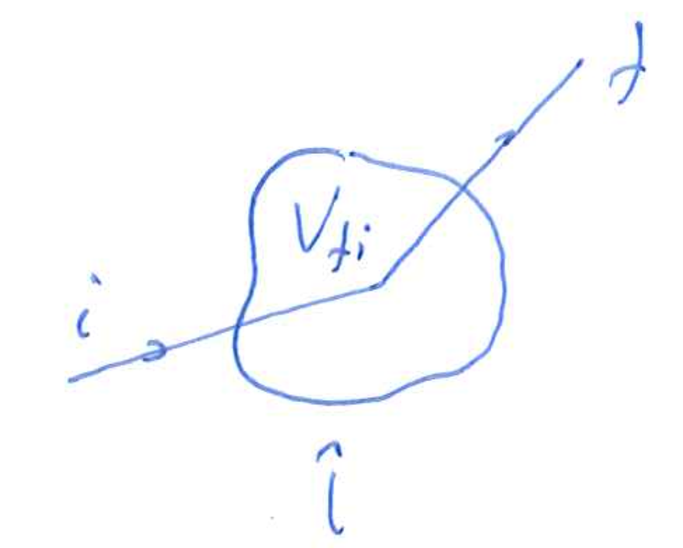
\includegraphics[scale=0.3]{Figures/firstorder.pdf}
    \caption{Picture of a scattering interaction at first order in the perturbative calculation.}
    \label{quantum-scattering:fig2}
\end{figure}
At second order, the interaction happens through an intermediate state $k$, as represented in Fig. \ref{quantum-scattering:fig3}.
\begin{figure}[h]
    \centering
    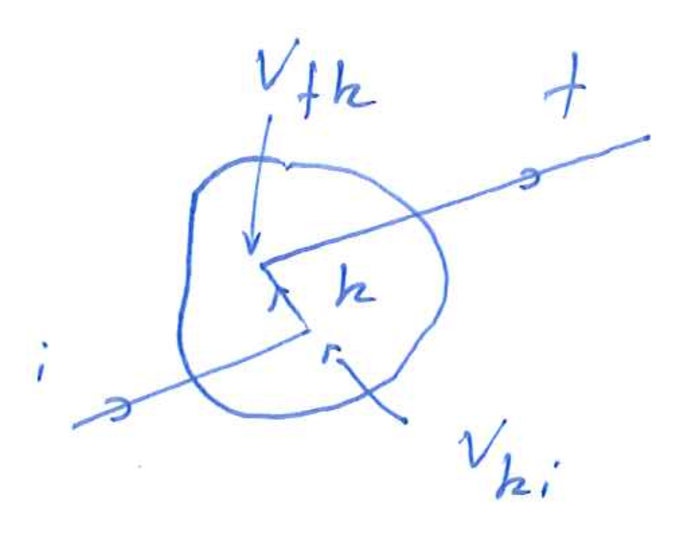
\includegraphics[scale=0.3]{Figures/secondorder.pdf}
    \caption{Picture of a scattering interaction at second order in the perturbative calculation: the scattering happens through an intermediate state $k$.}
    \label{quantum-scattering:fig3}
\end{figure}
The potential describing each interaction is denoted with subscripts, e.g. $V_{fi} = \langle f | V | i \rangle$ for the direct interaction between the initial and final state (same holds for $V_{fk}$ and $V_{ki}$).

In this representation, when a particle is scattered in a potential, there is a  momentum exchange between two particles through the potential, which is called a ``ranged interaction''. If the potential is created by a particle (e.g. a gold nucleus in the Rutherford experiment), during the ranged interaction the potential should  change instantly, but this would not be possible due to special relativity.

A new formulation of the process can be obtained thinking of the interaction as if were mediated by a \emph{mediator particle} $X$, as shown in Fig. \ref{quantum-scattering:fig4}. Let us also include the time in our ``picture'' of an interaction: for example, let's take an interaction $a+b\rightarrow c+d$
\begin{figure}
    \centering
    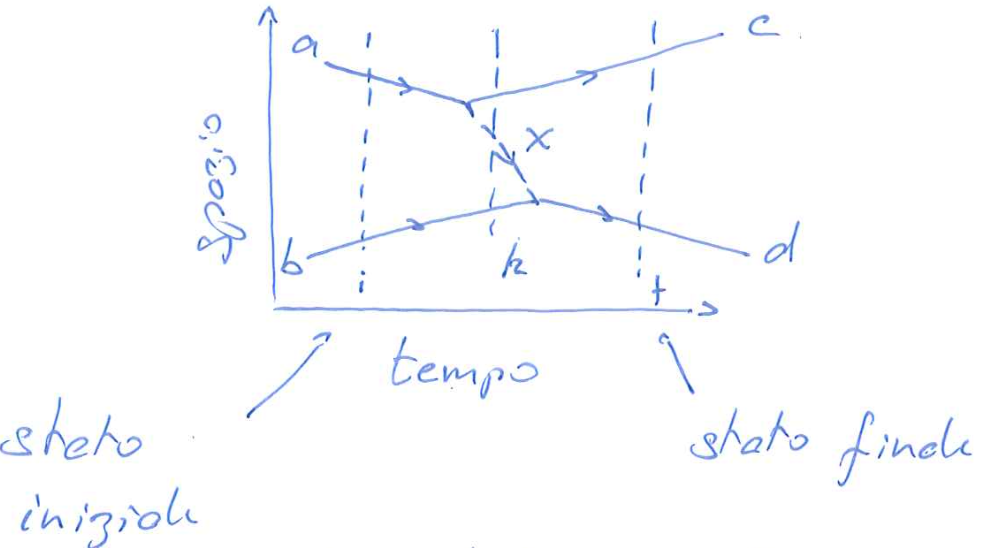
\includegraphics[scale=0.5]{Figures/qscat2.pdf}
    \caption{Picture of a possible, mediated interaction which brings from an initial state of two particles $a+b$ to a final state $c+d$. The horizontal axis represents time, while the vertical axis represents space, and the interaction between particles is mediated by a mediator $X$. In this specific picture, the $a$ particle emits $c$ together with $X$, which is then absorbed by $b$ which emits $d$.}
    \label{quantum-scattering:fig4}
\end{figure}
where the intermediate state is $k$. We will also assume that the interaction is quite simple: the transition matrix between any state is represented by a constant \emph{coupling} $g$, defined as
\[\langle k |V|i\rangle = g=\langle f |V|k\rangle,\]
as shown in Fig. \ref{quantum-scattering:fig5}. In this example, one way in which we can write the initial, intermediate and final states in terms of their particle content is
\begin{equation*}
    i:\,\,a+b,  \,\,\,\,\,\,\,\,\, k:\,\,c+x+b,\,\,\,\,\,\,\,\,\, f:\,\,c+d.
\end{equation*}
We can see this as the following time sequence:
\begin{enumerate}
    \item in the initial state $i$, we have the particles $a$ and $b$;
    \item the intermediate state $k$, where the particle $a$ emits a particle $X$ and a particle $c$, which exist together with $b$;
    \item the final state $f$, where $b$ has absorbed $X$ and emitted $d$, and so we are left only with $c$ and $d$.
\end{enumerate}
    
\begin{figure}[h]
    \centering
    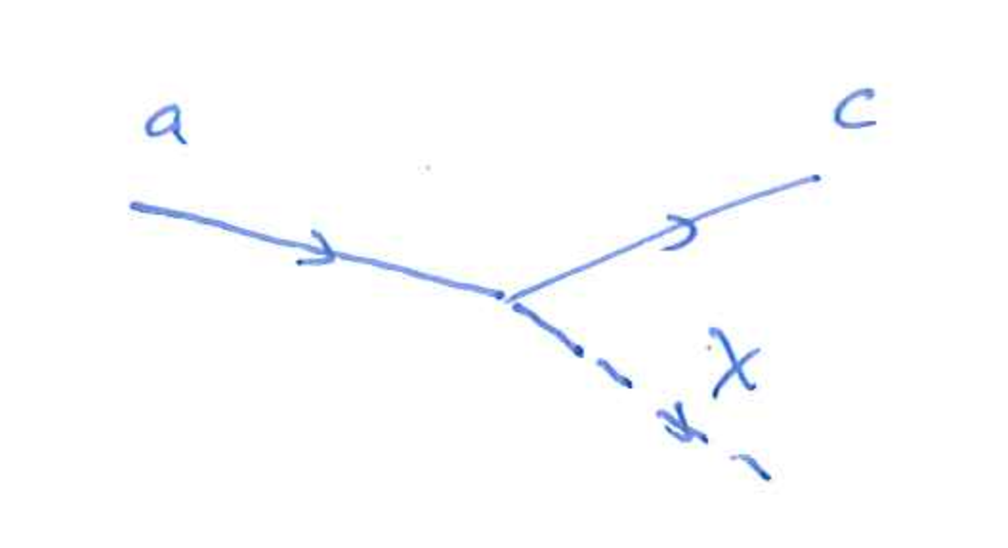
\includegraphics[scale=0.2]{Figures/qscat3.pdf}
    \caption{Simple interaction with a constant coupling $g$ between two quantum states $a$ and $c$; $X$ is the  particle which mediates their interaction (``mediator'').}
    \label{quantum-scattering:fig5}
\end{figure}

In this case, we have the transition matrix element
\begin{equation*}
    T_{fi}^{(i)} = \frac{\langle f | V | k\rangle\langle k | V | i \rangle}{E_{i}-E_{k}},
\end{equation*}
where the superscript $i$ is to remind us that we are considering \emph{one} possible option ($a$ emits $X$ and subsequently $b$ absorbs it).
The energies of the three states, in this specific hypothesis of what's going on in the interaction, are
\begin{align*}
        E_{i} = E_{a}+E_{b},\\
        E_{k} = E_{c}+E_{X}+E_{b},\\
         E_{f} = E_{c}+E_{d}.
\end{align*}
We use the assumption that $V_{lm}=g$ does not depend on the states $l$ and $m$, and write
\begin{equation*}
    T_{fi}^{(i)} = \frac{g^2}{(E_{a}+E_{b}) - (E_{c}+E_{x}+E_{b})} = \frac{g^2}{E_{a}-E_{c}-E_{x}}.
\end{equation*}

But, in the sum of Eq. \eqref{eq:reminderTfi}, we need to consider all possible intermediate states, even the ones in which $b$ emits $X$ and $a$ absorbs it, as it is shown in Figure \ref{quantum-scattering:fig6}. This is a crucial point!
\begin{figure}
    \centering
    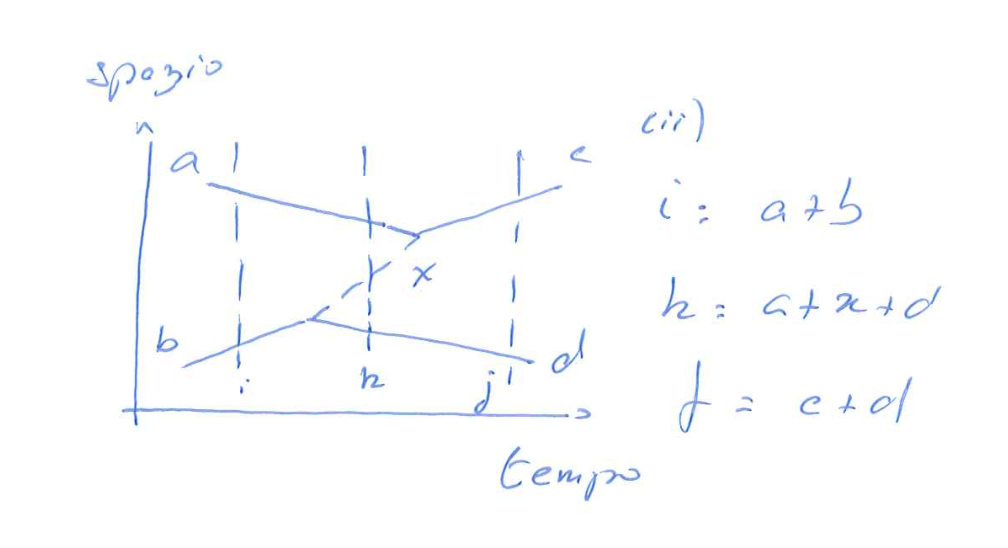
\includegraphics[scale=0.5]{Figures/qscat4.pdf}
    \caption{Picture of an alternative interaction between $a$ and $b$, which leads to a final state $c+d$. In this specific picture, the $b$ particle emits $d$ together with $X$, which is then absorbed by $a$ which emits $c$.}
    \label{quantum-scattering:fig6}
\end{figure}
In this case we have
\begin{align*}
        &E_{i} = E_{a}+E_{b},\\
        &E_{k} = E_{a}+E_{X}+E_{d},\\
         &E_{f} = E_{c}+E_{d},
    \end{align*}
from which one gets
\begin{equation*}
    T_{fi}^{(ii)} = \frac{g^2}{E_b-E_d-E_X},
\end{equation*}
again with a superscript $ii$ which reminds us the fact this is another term in the sum of Eq. \eqref{eq:reminderTfi}.
Since the energy conservation can be written as
\begin{equation*}
    E_a + E_b = E_c + E_d \,\,\,\,\rightarrow\,\,\,\, E_b = E_c + E_d - E_a,
\end{equation*}
we can write
\begin{equation*}
    T_{fi}^{(ii)} = \frac{g^2}{E_c-E_a-E_X}.
\end{equation*}

The sum of these two contributions is
\begin{equation*}
    T_{fi}^{(i)} + T_{fi}^{(ii)} = g^2 \left( \frac{1}{E_a-E_c-E_X} - \frac{1}{E_a-E_c+E_X} \right) = \frac{2g^2E_X}{(E_a-E_c)^2-E_X^2}.
\end{equation*}
From the relativistic energy-momentum-mass relation we can write
\begin{equation*}
    E_X^2 = p_X^2 + M_X^2,
\end{equation*}
where $\Vec{p_X} = \Vec{p_a} - \Vec{p_c}$ (i.e. we assumed the conservation of momentum in the process $a\to X+c$). Therefore,
\begin{equation*}
    E_X^2 = (\Vec{p_a} - \Vec{p_c})^2 + M_X^2.
\end{equation*}

If we define the four-momenta $q$, $p_a$ and $p_c$, we have
\[q = p_a - p_c,\]
from which we can write
\begin{equation*}
    T_{fi} = 2E_X \frac{g^2}{(E_a-E_c)^2 - (\Vec{p_a} - \Vec{p_c})^2 - M_X^2},
\end{equation*}
and since $(E_a-E_c)^2 - (\Vec{p_a} - \Vec{p_c})^2 = q^2$, we have
\begin{equation*}
    T_{fi} = 2E_X \frac{g^2}{q^2-M_X^2}.
\end{equation*}
The term
\begin{equation*}
    \frac{1}{q^2 - M_x^2}
\end{equation*}
is called the \emph{propagator of the interaction}.% (or of the interaction particles).
The term $g$ is called the \emph{coupling} of the interacting particles to the mediator of the interaction itself.

Note that the term $T_{fi}$ is not a Lorentz invariant, due to the presence of the term $2E_X$. The term
\begin{equation*}
    \frac{g^2}{q^2-M^2}
\end{equation*}
is instead a Lorentz invariant. The interaction rate must necessarily not depend on the reference frame we use to describe the interaction, while the term $2E_X$ does depend on the normalisation chosen for the wave functions during the perturbation calculation. In fact, choosing a different normalisation (which in quantum mechanics, we stress it, cannot affect the results of any physical measurements) we can absorb the $2E_X$ term: we can in fact require that the space integral of the free-particle wave functions is
\begin{equation*}
    \int_V \Phi^*\Phi\,d^3x = 2E_X,
\end{equation*}
instead of $1$.

One should also note that it is necessary to maintain the chosen order of perturbation theory for all the considered intermediate configurations of the system.
The higher order of perturbation we apply, the more intermediate configuration are possible; in particular, these two numbers coincide.

\section{Feynman diagrams}
The calculations of cross-sections and decay rates in particle physics is performed using a different formalism in relativistic quantum mechanics and quantum field theory. A representation of the calculations can be given through the use of \emph{Feynman's diagrams}, in which the perturbations which were ordered in time are instead represented by single diagrams, as shown in Fig. \ref{quantum-scattering:fig7}.
\begin{figure}[h]
    \centering
    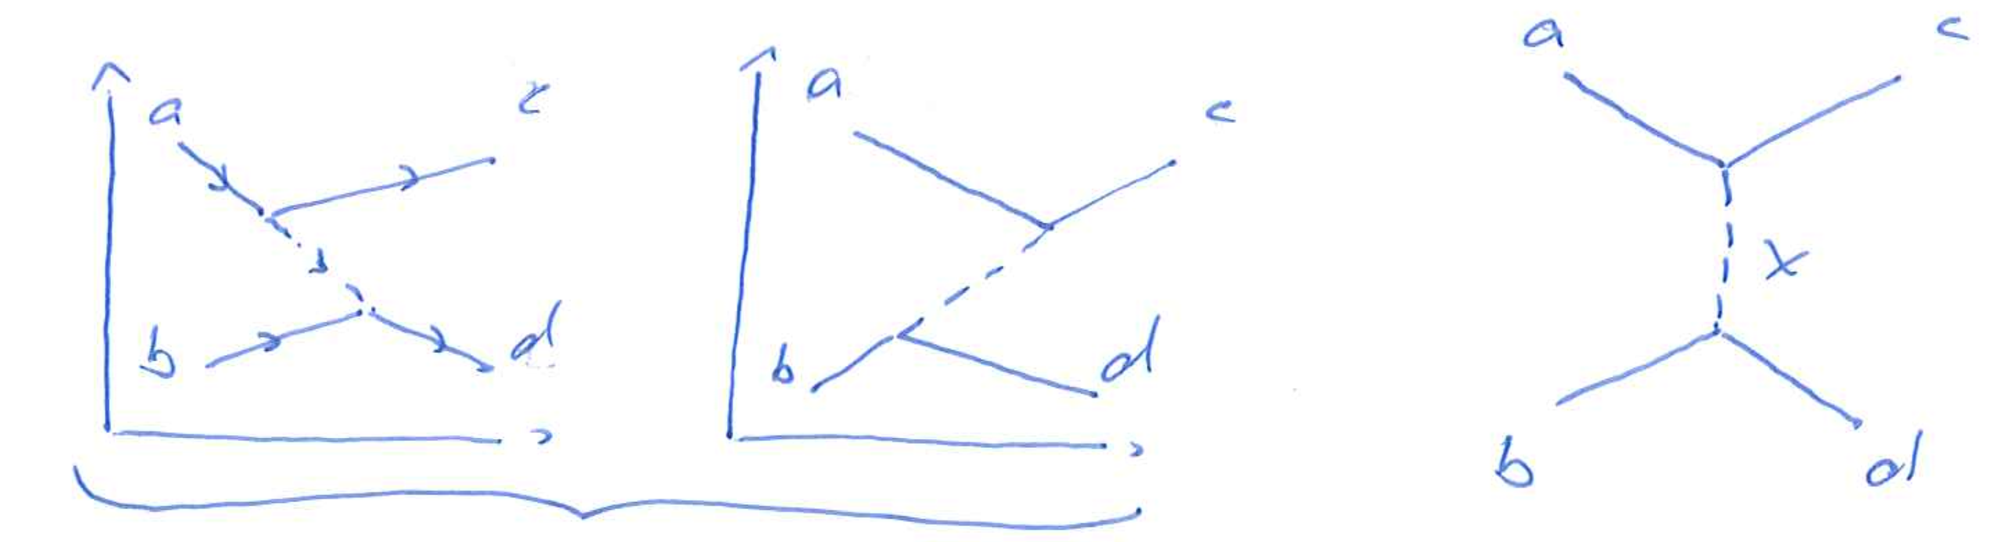
\includegraphics[scale=0.32]{Figures/qscat5}
    \caption{The alternative interactions which were ordered in time in perturbation theory, shown by the left diagrams, are replaced by a single Feynman diagram, shown on the right.}
    \label{quantum-scattering:fig7}
\end{figure}

As shown in the case of perturbation theory, in the interaction ``vertices'' the energy is not conserved and the $X$ particle, the mediator, is considered as a physical particle which may be measured/observed. In the Feynman diagram formalism, instead, the mediator is considered as an ``intermediate'' state with a \emph{virtual mass} $q^2$ which does not correspond to the mass of the free particle, $M_X^2$ ($q^2\neq M_X^2$); but the four-momentum is conserved at the vertices. A virtual particle can be seen as a mathematical construct which represents the sum over all the possible time ordering considered by perturbation theory.

Both representations are equivalent. The ``classical'' interpretation with the exchange of a physical intermediate particle fulfills the interpretation of the momentum transfer.

\section{Density of states, wave function normalisation and phase space}
How can we calculate the density of states, which is needed in order to obtain the transition rate from an initial and a final state according to Fermi's golden rule? We start from the fact that the wave function of a free particle is given by
\begin{equation*}
    \psi(\Vec{x},t) = Ae^{i\Vec{p}\cdot\Vec{x}-iEt},
\end{equation*}
and its normalisation is usually obtained requiring
\begin{equation*}
    \int_{V}d^3x \psi^*\psi = 1,
\end{equation*}
which corresponds to one particle in the volume $V$. This is an important element to consider. In the case of a free particle (plane wave), in a cubic volume $V$ with side $a$ (i.e. a box) we therefore have
\begin{equation*}
    \int_0^a\int_0^a\int_0^a\psi^*\psi\,dx\;dy\;dz\, = 1.
\end{equation*}
The normalisation of the wave function $A$ is therefore
\begin{equation*}
    A^2 = \frac{1}{a^3} = \frac{1}{V}.
\end{equation*}
This normalisation implies that the wave function satisfies the boundary conditions 
\begin{equation*}
    \psi(x+a,y,z) = \psi(x,y,z) = \psi(x,y+a,z) = \psi(x,y,z+a).
\end{equation*}
Taking a volume $V$ with periodic boundary conditions is equivalent to the case of  wave functions which vanish at the borders of a box, but allows easier calculations with momenta.

We want to count the number of possible states for given energy or momentum. Let's start with momentum: the periodic boundary conditions applied to the $x$ direction imply that
\begin{equation*}
    e^{ip_xx} = e^{ip_x(x+a)},
\end{equation*}
and similarly for the $y$ and $z$ directions. Therefore, from the requirement $e^{ip_xa} = 1$ we have that $p_xa$ must be a multiple of $2\pi$; this implies
\begin{equation*}
    (p_x,p_y,p_z) = \frac{2\pi}{a}(n_x,n_y,n_z),
\end{equation*}
where $n_x, n_y, n_z$ are integers.
In other words, not all momentum values are allowed, and the momentum space is quantized, as shown in Fig. \ref{quantum-scattering:fig8}.
\begin{figure}[h]
%    \centering
    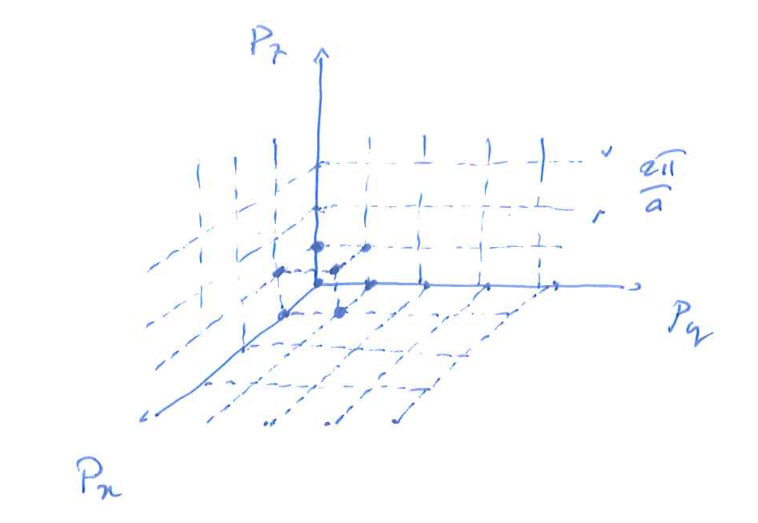
\includegraphics[scale=0.36]{Figures/qscat6}
    \caption{Quantization of the momentum space. Any particle lives in a point of this three-dimensional grid.}
    \label{quantum-scattering:fig8}
\end{figure}

In order to count the number of states with momentum in the range $[p,p+dp]$, we have to perform a calculation over a 3D sphere in the $(p_x,p_y,p_z)$ space;  Fig. \ref{quantum-scattering:fig9}  shows a projection of this sphere on the $(p_x,p_y)$ plane.
\begin{figure}[h]
    \centering
    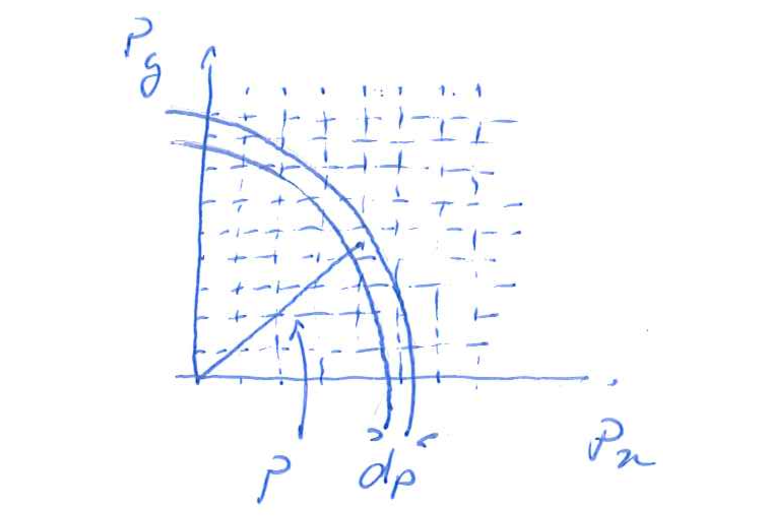
\includegraphics[scale=0.4]{Figures/qscat7}
    \caption{Projection over the $(p_x,p_y)$ plane of the quantisation of the space of the momenta.}
    \label{quantum-scattering:fig9}
\end{figure}
Every single state occupies a cubic volume
\begin{equation*}
    d^3p = dp_x\,dp_y\,dp_z\, = \left(\frac{2\pi}{a}\right)^3 = \frac{(2\pi)^3}{V},
\end{equation*}
therefore the number of states with momentum $p \in [p,p+dp]$ will be equal to the ratio between the volume between two spheres with a radius differing by $dp$, $4\pi p^2dp$, divided by the volume occupied by a single state:
\begin{equation*}
    dn = 4\pi p^2 dp\left(\frac{V}{(2\pi)^3}\right).
\end{equation*}
This leads to
\begin{equation*}
    \frac{dn}{dp} = \frac{4\pi p^2}{(2\pi)^3}V.
\end{equation*}
We can in turn write the density of states as
\begin{equation}\label{eq:dennedp}
    \rho(E) = \frac{dn}{dE} = \frac{dn}{dp}\left|\frac{dp}{dE}\right|.
\end{equation}
From the last term of the right-hand side of this equation, one can see that decays to lighter particles are more probable (have higher density of states) than decays to heavier particles.

Again, the interaction rate will not depend on the overall normalisation, which cancels out with the other terms from Fermi's golden rule: the normalisation of the waveform is $1/\sqrt{V}$, and its square appears in the transition matrix element squared, which cancels out with the factor $V$ in Eq. \eqref{eq:dennedp}.
To simplify the calculations we can take therefore an unitary volume, $V=1$, choosing a normalisation which corresponds to one particle per volume unit.

For a solid angle element $d\Omega$, the density of the states can be expressed using spherical coordinates as\footnote{We simply used the fact that the volume element in spherical coordinates is $r^2drd\Omega=r^2dr\sin\theta d\theta d\phi$.}
\begin{equation*}
    dn = p^2\sin{\theta}\,dpd\theta d\phi \frac{V}{(2\pi)^3},
\end{equation*}
therefore
\begin{equation*}
    \frac{dn}{dp} = \frac{p^2\sin{\theta}dpd\theta d\phi}{(2\pi)^3}V.
\end{equation*}
For a final state with $N$ particles, there will be $N-1$ independent momenta (due to momentum conservation), therefore we need to count $N-1$ final states:
\begin{equation*}
    dn = \prod_{i=1}^{N-1}dn_i = \prod_{i=1}^{N-1}\frac{d^3p_i}{(2\pi)^3}V.
\end{equation*}

In the case of a decay of a particle into $N$ particles, $a\to b_1+b_2+\dots + b_n$, the number of independent states can be expressed in terms of all $N$ particles in the final state, by using a Dirac delta to impose the conservation of momentum:
\begin{equation*}
    dn = (2\pi)^3\prod_{i=1}^{N}\frac{d^3p_i}{(2\pi)^3}\delta^3\left(\vec{p}_a-\sum_{i=1}^N \vec{p}_i\right) V.
\end{equation*}

\section{Cross-section and decay rate}
The concept of cross section is related to the transition rate (or interaction rate) in the case of a beam of particles $A$ which interact with a target of particles $B$, through the relation
\begin{equation*}
    \frac{dN_i}{dt} = \sigma\Phi_A N_B,
\end{equation*}
where $\Phi_A$ is the flux of $A$ particles, and $N_B$ is the number of targets accessible to the beam. Considering a particle density $n_A$ and a velocity of the beam $v_A$, we have seen that one can write
\begin{equation*}
    \Phi_A = n_A v_A.
\end{equation*}
The cross-section is the equivalent surface for a single particle target of the interaction
\begin{equation*}
    \sigma = \frac{1}{\Phi_A N_B}\times \frac{dN_I}{dt}.
\end{equation*}

The rate $\Gamma_{fi}$ is defined by the Fermi's golden rule: for a specific scattering corresponds to
\begin{equation*}
    %\frac{d\sigma}{d\Omega}
    \sigma= \frac{\Gamma_{fi}}{\Phi_A} = \frac{2\pi}{\hslash}\frac{|T_{fi}|^2\rho(E_{i})}{\Phi_A},
\end{equation*}
and depends on $\rho(E_i)$ (the density of states, a function of the initial state energy $E_i$) and $\Phi_A$, which must be evaluated correctly.

In the case of particle decays, instead, the decay rate $\Gamma_{fi}$ is directly given by Fermi's golden rule.

\section{Electromagnetic interaction - the Rutherford scattering}
Let's consider a simple case for which we know the classical cross-section, the Rutherford scattering, which is the scattering of a charged particle by an electrostatic potential
\begin{equation*}
    V_{C}(r) = \frac{Ze}{4\pi\epsilon_0r}.
\end{equation*}
Our goal is to compute the cross-section in quantum mechanics, using the time-dependent perturbation theory we developed in the last sections.

Let us consider again a beam of  $\alpha$ particles, with a charge $Ze$, mass $m$ and momentum $\Vec{p_i}$. Given the typical energy of $\alpha$ particles, the problem -- as we have seen -- is non-relativistic.
 We will choose a normalisation of the wave function corresponding to $1$ particle per unit volume, so that we will have $n_A = 1$, and $\Phi_{A} = v_{A} = \frac{p_i}{m}$. We will call $\Vec{p}_f$ the final state momentum and $\theta$ the angle between the initial and final directions of the momentum (the ``scattering angle'').
\begin{figure}[h]
    \centering
    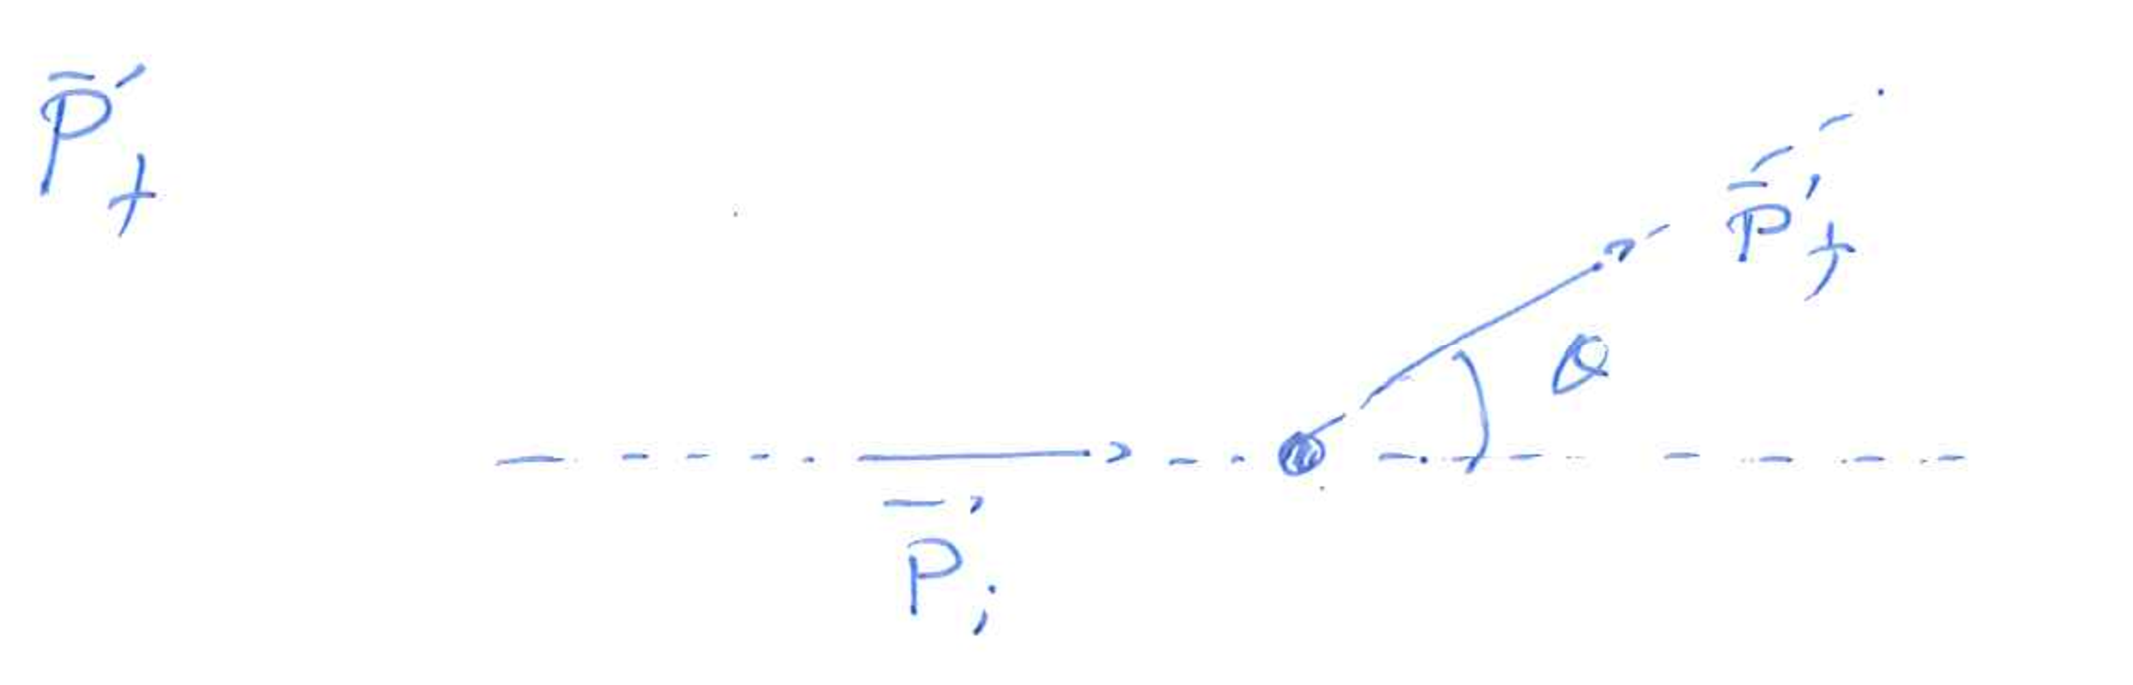
\includegraphics[scale=0.25]{Figures/qscat8}
    \caption{Relation between initial and final state momenta and scattering angle of an $\alpha$ particle in the Rutherford scattering experiment.}
    \label{fig:qscat-fig8}
\end{figure}

Fermi's golden rule is
\begin{equation*}
\Gamma_{fi} = \frac{2\pi}{\hslash} |T_{fi}|^2 \rho(E_i),
\end{equation*}
where $\rho(E_{i})$ is the density of the final states (given the initial state energy) included in the solid angle $d\Omega_f$. We have
\begin{equation*}
    \frac{dn}{dp} = \frac{p^2\sin{\theta}d\theta d\phi}{(2\pi)^3},
\end{equation*}
and since in the initial and final state the $\alpha$ particle is free, we have
\begin{equation*}
    E_{f} = \frac{p_f^2}{2m},
\end{equation*}
so that we can write
\begin{equation*}
    \frac{dE_f}{dp_f} = \frac{p}{m}.
\end{equation*}

The wave functions of the initial and final states, normalised to $1$, are
\begin{equation*}
    \psi_i = e^{i(\Vec{p_i}\cdot\Vec{r} - Et)}\;\;\;\;\;\;\;\psi_f = e^{i(\Vec{p_f}\cdot\Vec{r}-Et)},
\end{equation*}
therefore
\begin{equation*}
    T_{fi} = \int_{V}d\Vec{x} \psi_{f} V(r)\psi_i.
\end{equation*}
Note that in this case $V(r)$ is the \emph{potential energy}, not the Coulomb potential:
\begin{equation*}
    V(r) = -ze\frac{Ze}{4\pi\varepsilon_0 r}.
\end{equation*}
Using the conservation of energy ($E_f=E_i$), we obtain
\begin{equation*}
    T_{fi} = -\frac{zZe^2}{4\pi\varepsilon_0}\int_{0}^{\infty}\int_{0}^{\pi}\int_{0}^{2\pi}r^2\sin{\tilde{\theta}}e^{i\Vec{q}\cdot\Vec{r}}\frac{1}{r}drd\tilde{\theta}d\phi,
\end{equation*}
where $\Vec{q} = \Vec{p_i} - \Vec{p_f}$, and $\tilde{\theta}$ is the polar angle in the direction $\Vec{q}$ (not to be confused with the polar scattering angle $\theta$).

Therefore, we can write
\begin{equation*}
    \frac{-zZe^2}{4\pi\varepsilon_0}\int_{0}^{\infty}\int_{0}^{\pi}\int_{0}^{2\pi}r^2\sin{\tilde{\theta}}e^{iqr\cos\tilde{\theta}}\frac{1}{r}drd\tilde{\theta}d\phi.
\end{equation*}
We define $y = \cos{\tilde{\theta}}$, so that we have
\begin{equation*}
    dy = -\sin{\tilde{\theta}}d\tilde{\theta},
\end{equation*}
and then performing the integral over $\phi$, obtaining
\begin{equation*}
    T_{fi} = \frac{zZe^2}{4\pi\varepsilon_0}2\pi\int_{0}^{\infty}\int_{-1}^{-1}r^2e^{iqry}\frac{1}{r}drdy = \frac{zZe^2}{4\pi\varepsilon_0}2\pi\int_{0}^{\infty}r\left[\int_{-1}^{1}e^{iqry}dy\right]dr.
\end{equation*}

Since
\begin{equation*}
    \int_{-1}^{1}e^{iqry}dy = \frac{e^{iqr}-e^{-iqr}}{iqr} = 2\frac{\sin{(qr)}}{qr},
\end{equation*}
we have (assuming $\hslash=c=1$)
\begin{equation*}
    \begin{split}
        T_{fi} & = \frac{zZe^2}{4\pi\varepsilon_0}2\pi\int_{0}^{\infty}\frac{2i}{qi}\sin{(qr)}dr = 4\pi zZ\alpha\frac{1}{q}\int_{0}^{\infty}\sin(qr)dr = \\
        & = 4\pi zZ\alpha \frac{1}{q}\left[\frac{e^{iqr}+e^{-iqr}}{iq\cdot2i}\right]_{0}^{\infty}.
    \end{split}
\end{equation*}

We can consider that the potential is shielded for large enough distances, and therefore introduce a term $e^{-\varepsilon r}$ for which we take
\begin{equation*}
    \frac{1}{r}\rightarrow \lim_{\varepsilon\rightarrow0}\frac{e^{-\varepsilon r}}{r}.
\end{equation*}
The oscillating term in the integral we need to solve to calculate $T_{fi}$ becomes
\begin{equation*}
    \lim_{\varepsilon\rightarrow 0}\int_{0}^{\infty}e^{-\varepsilon r}\sin{(qr)}dr = \lim_{\varepsilon\rightarrow 0}\left[\frac{e^{iqr-\varepsilon r}}{(iq-\varepsilon )2i}-\frac{e^{-iqr-\varepsilon r}}{(-iq-\varepsilon)2i}\right]_{0}^{\infty},
\end{equation*}
so
\begin{equation*}
    \lim_{\varepsilon\rightarrow 0}\int e^{-\varepsilon r}\sin{qr} dr = \lim_{\varepsilon \rightarrow 0}\frac{q}{q^2+\varepsilon^2} = \frac{1}{q},
\end{equation*}
and in the end we get
\begin{equation*}
    T_{fi} = 4\pi\alpha z Z \frac{1}{q^2}.
\end{equation*}
We get the given form of the matrix element which includes the product of two numbers, $ze$ and $Ze$ (``couplings''), and a ``\emph{propagator}" of the form $\frac{1}{q^2-M_X^2}$, where $M_X = 0$ (the massless photon).
The transferred momentum can be expressed as
\begin{equation*}
    q^2 = |\Vec{p_i} - \Vec{p_f}|^2 = 2p_i^2(1-\cos{\theta}),
\end{equation*}
where $p_i = p_f$ (in general the scattering is elastic and the nucleus does not move), and $p_i^2 = p_f^2 = 2mE$ ($E$ is the kinetic energy of the $\alpha$ particle), therefore
\begin{equation*}
    q^2 = 8mE\sin^2\left(\frac{\theta}{2}\right),
\end{equation*}
where we used
\begin{equation*}
    1-\cos{\theta} = 2\sin^2\left(\frac{\theta}{2}\right).
\end{equation*}

For the cross section we have
\begin{equation*}
    d\sigma = \frac{\Gamma_{fi}}{\Phi_A} = \frac{2\pi|T_{fi}|^2\rho(E_i)}{p_i/m},
\end{equation*}
where 
\begin{equation*}
    \rho(E_i) = \frac{p_i^2\sin{\theta}d\theta d\phi}{(2\pi)^3}\times\left(\frac{dp}{dE}\right) = \frac{p_i^2d\Omega}{(2\pi)^3}\frac{m}{p_i}.
\end{equation*}
The differential cross-section can then be written as
\begin{equation*}
    \frac{d\sigma}{d\Omega} = \frac{1}{(2\pi)^2}T_{fi}^2m^2 = \frac{1}{(2\pi)^2}(4\pi)^2\times(\alpha zZ)^2\times\frac{1}{64E^2\sin^4\frac{\theta}{2}},
\end{equation*}
and in the end
\begin{equation*}
    \frac{d\sigma}{d\Omega} = \frac{(\alpha zZ)^2}{16}\frac{1}{E^2\sin^4\frac{\theta}{2}},
\end{equation*}
which is the Rutherford cross section, the same of the classical calculation!

\section*{Take-home lessons}
\begin{itemize}
    \item One of the keys of scattering theory is that we consider particles at infinite distance from the region where a potential acts as \emph{free particles}, which can then be described with plane waves, i.e. positive-energy solutions of the free-particle Schr\"oedinger equation. Negative-energy solutions instead represent (in non-relativistic quantum mechanics) bound states.
    \item In quantum mechanics, a different choice on the normalisation of a wave function must have no effect on calculated physical quantities (like cross-sections). Probability current can then be interpreted in terms of the flux of particles of a beam.
    \item In time-independent perturbation theory (i.e. if the Hamiltonian of a system does not depend on time), and in the presence of a central potential in a three-dimensional space, it is convenient to express the Schr\"oedinger equation in terms of the sperical expression of the Laplacian operator $\nabla^2$. In this way, its solutions can be separated into a radial and an angular part. The wave function can then be expanded in partial waves, i.e. projected onto the basis formed by the Legendre polynomials: one finds that a plane wave can ve decomposed into two spherical waves, one propagating outwards and one inwards. 
    \item In general, the Hamiltonian of a system may depend on time, and one would have to use the time-dependent perturbation theory to get an approximated solution of the Schr\"oedinger equation. The solution to this equation can be expressed in the basis of the solutions of the free-particle Hamiltonian, in terms of coefficients which are time-dependent. If the perturbative potential is weak, one can find an expression of the transition probability between two states of the system (which in the end is a concept related to the scattering cross-section!), and use this to calculate the total transition probability. This latter quantity in turn depends on the density of accessible states.
    \item If one brings time perturbation theory to second order, one can see (Fermi's Golden Rule) that the transition matrix between the initial and final state depends on a sum over possible intermediate states $k$, so that the transition $i\to f$ is actually $i\to k \to f$. This sum should run over \emph{all} possible intermediate states: an interaction $a+b\to c+d$ can then be seen as mediated by the exchange of another particle $x$, which implies a contribution to the transition matrix which depends on its mass $M_x$ and on a coupling strength factor $g$ which "weighs" the interaction with $x$.
    \item Feynman diagrams represent a convenient way to visualize this summation over possible intermediate states. They prove essential to compute cross-sections in Relativistic Quantum Mechanics and Quantum Field Theory.
    \item The density of states represents the volume density of accessible states in the momentum space. It is a quantity which depends on energy-momentum conservation -- a final state with $N$ particles will have only $N-1$ independent momenta, as the total momentum is constrained to be equal to the initial state value.
    \item The Golden Rule allows to express the interaction rate in terms of the square of the transition matrix between initial and final state, and of the density of states.
    \item The quantum-mechanical calculation of the differential cross-section of Rutherford scattering yields the same results as the classical calculation.
\end{itemize}
\section*{Questions}
\begin{itemize}
    \item In quantum mechanics, are energy eigenvalues always quantised?
\end{itemize}

%%%%%%%%%%%%%%%%%%%%% chapter.tex %%%%%%%%%%%%%%%%%%%%%%%%%%%%%%%%%
%
% sample chapter
%
% Use this file as a template for your own input.
%
%%%%%%%%%%%%%%%%%%%%%%%% Springer-Verlag %%%%%%%%%%%%%%%%%%%%%%%%%%
%\motto{Use the template \emph{chapter.tex} to style the various elements of your chapter content.}
\chapter{Interaction of Particles with Matter}
\label{chap:InteractionsInMatter}

Before more fundamental concepts in the development of the field of nuclear and subnuclear physics are discussed, it is important to introduce fundamental concepts of the interaction of particles in matter. Much of the progress in nuclear, subnuclear and particle physics required ingenious detection techniques of particles. By using just the notions of relativity and scattering theory discussed so far, we will be able to better understand the discoveries that have led to the greater understanding of the nucleus, the nuclear forces and of particles and fundamental interactions in general. 

Understanding particle properties requires particle detectors, and particle detectors are based on the interaction of particles in matter. 

The main properties that will characterize the particles of interest will be quite simple: their mass and kinematic properties and their electric charge. Their spin and magnetic moment will essentially play little role in the following and all the phenomena that will be quantitatively described result from the electromagnetic interaction alone.

It is conceptually simple to measure the momentum of a charged particle using a magnetic field. However, to do so it is important to be able to ``sense'' the presence of a particle and track it as precisely as possible. From the measurement of the momentum of the particle it is less obvious how the mass of the particle can be inferred. For this purpose, all possible properties of the interaction of charged particles in matter will be discussed. How neutral particles can be detected and their energy measured will also be addressed. 

In order to efficiently describe the interaction of particles in matter, this chapter will focus on the loss of energy of particles in matter. The following aspects will be covered.

A charged particle which is crossing a material can lose its energy by:
\begin{itemize}
\item Ionization or excitation of other atoms;
\item Coulomb--scattering with atomic nuclei;
\item Radiation emission in the field of atomic nuclei (\emph{Bremsstrahlung}).
\end{itemize}

A photon interacting with matter can lose its energy via:
\begin{itemize}
\item Photoelectric effect;
\item Compton scattering;
\item Production of electron--positron pairs.
\end{itemize}



\section{The Bohr Atom}
At the end of the XVIII century, experiments had shown
that excited gaseous elements could emit radiation, and different spectral
lines were associated to different elements. Discrete emission lines, with well-defined patterns, were first observed by Johann Balmer in 1885. While Thomson's plum pudding model was coherent with the knowledge of the
time that atoms were known to be electrically neutral and to be composed
of electrons, this model could not provide an explanation for the existence of these lines.

It was really Rutherford's experiment that demonstrated that atoms are composed of positively-charged nuclei, surrounded by electrons. At the time it was already clear that the hypothesis was lacking an explanation for the nature of atomic nuclei: given how small the nuclei seemed to be, how could all the positive charges be kept together against the strong electrostatic repulsion? Well before the secrets of the nucleus were unveiled, the Rutherford model could be used to build more accurate models of the atom.

In 1913, Bohr who had been working with Rutherford, developed his famous atomic model based on the following assumptions:
\begin{itemize}
\item an hydrogen atom is composed by a proton and an electron, kept
  together by the Coulomb potential;
\item the mass of the proton is much greater than the mass of the
  electron;
\item the atom is stationary: electrons revolve in stationary orbits
  around the nucleus and do not radiate energy.
\end{itemize}
Let's assume that the orbits are circular. If $m$ is the mass of the
electron, then
\begin{equation}
  \label{eq:bohr1}
  F=\frac{e^2}{4\pi\epsilon_0 r^2} = m\omega^2 r,
\end{equation}
and the energy of the system is constant and given by:
\begin{eqnarray*}
  E &=& \frac{1}{2}m\omega^2 r^2 - \frac{e^2}{4\pi\epsilon_0 r}\\
    &=& \frac{1}{2}\rr{\frac{e^2}{4\pi\epsilon_0r}} - \frac{e^2}{4\pi\epsilon_0 r}\\
    &=&  -\frac{1}{2}\,\frac{e^2}{4\pi\epsilon_0 r}.
\end{eqnarray*}

Also, if the orbits are stationary, the angular momentum is conserved,
\[L = m\omega r^2 = \text{const}.\]

Bohr introduced the assumption that the angular momentum is quantized,
\[\oint L\ d\phi = n h,\]
where $h$ is the Planck' constant. In another way, one has
\[L = n\hslash = n\frac{h}{2\pi},\]
which fixes the allowed values of the
energy and radius of the electron orbits. From Eq. \eqref{eq:bohr1} we easily get the
quantisation rule for the radius:
\begin{align*}
  m\omega^2r^4 &=\frac{e^2 r}{4\pi\epsilon_0 },\\
  \frac{L^2}{m} &=  \frac{e^2 r}{4\pi\epsilon_0 },\\
  r &\equiv r_n  = \frac{n^2 \hslash^2}{\rr{\frac{me^2}{4\pi\epsilon_0}}},
\end{align*}
where used the subscript $n$ to highlight the fact that the radius $r_n$ is quantised. Similarly, for the energy we have
\[E_n = -m\frac{\rr{\frac{e^2}{4\pi\epsilon_0}}^2}{2n^2\hslash^2}.\]
Bohr's atomic model is also providing an explanation for the lines
appearing in the emission spectrum: lines appear in a discrete number, as a consequence of the quantization of the electronic
orbits. In fact, the wavelength emission is associated with the
 transition of an electron from the $m$-th orbit to the $n$-th orbit ($n<m$), which happens with the emission of a photon with an energy given by
equation:
\[h \nu = E_m - E_n.\]

Let's now introduce two fundamental constants which will be convenient to simplify notation in the theory of nuclear and particle physics. The fist one is the
\emph{fine--structure constant} $\alpha$, defined as
\[\alpha = \frac{e^2}{4\pi\epsilon_0\hslash c} \simeq \frac{1}{137},\]
and the second one is the \emph{classical electron radius} $r_e$, which is defines as
the radius of a charged sphere with electrostatic energy equal to
$m_ec^2$:
\[m_ec^2 = \frac{e^2}{4\pi\epsilon_0 r_e}.\]

Using these definitions, it is possible to write the two formulas for
$E_n$ and $r_n$ in the following way:
\begin{eqnarray*}
  E_n &=& -\frac{1}{2n^2}\alpha^2mc^2,\\
  r_n &=& n^2 \frac{r_e}{\alpha^2}.
\end{eqnarray*}
For the fundamental state of the hydrogen atom, we have
\begin{eqnarray*}
  E_1 &=& -13.6\ \electronvolt,\\
  a &=& r_1 = 0.53\ \times\ 10^{-10}\ \meter.
\end{eqnarray*}

The magnetic moment of a system can be expressed in terms of its angular momentum. If we see a particle as a coil of surface $S$ with a given electric current $i$, for example, its magnetic (dipole) moment will be given by
\begin{equation*}
  \vec{\mu} = i\vec{S}.
\end{equation*}
In the case of Bohr's model, we can calculate the magnetic moment associated to one orbit of the electron, by identifying
\begin{align*}
  \vec{S} &= \pi r^2 \hat{n},\\
  i &= e/T = e \nu = \frac{e\omega}{2\pi},
\end{align*}
where $T$ is the period of the orbit and $\nu=1/T=\omega/2\pi$ its frequency, and $\hat{n}$ is the unit vector orthogonal to the orbit plane. We then get
\begin{equation*}
  \vec{\mu} = \pi r^2 \frac{e{\omega}}{2\pi}\hat{n} = \frac{e\vec{L}}{2m},
\end{equation*}
from which one can define another fundamental constant, the \emph{Bohr magneton}, which is the magnetic moment of the fundamental state of the hydrogen atom:
\begin{equation*}
  \mu_B = \frac{e\hslash}{2m} = 5.8\times 10^{-5}\ \electronvolt / \tesla.
\end{equation*}
The Bohr magneton is naturally used as the unit for expressing the magnetic moment of fundamental particles. The above expression is of course valid only in the international system of units (and remember that here $m$ is the electron mass!).

\section{Energy loss by ionization}
\subsection{The Bohr formula}\label{sec:energyLossBohr}
It is interesting to take a closer look at the derivation of the energy loss of a charged particle in a material using some of the concepts discussed in Chapter~\ref{Scattering-1}.

To do so we consider an atom with $Z$ electrons and a nucleus with a
charge equal to $Ze$, and an interacting particle with charge $ze$ and mass $M$ typically larger than the mass of the electron $m_e$. A picture of the interaction of the particle with an electron of the atom is given in Fig.~\ref{fig:passRadMat1}. 

\begin{figure}
  \centering 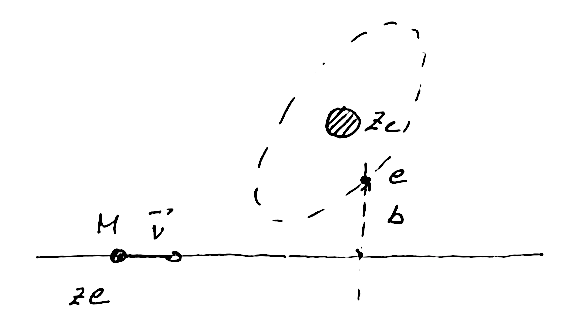
\includegraphics[width=0.5\textwidth]{passRadMat1.png}
  \caption{Illustration of the interaction of a particle of mass $M$ and charge $ze$ with an electron of an atom with atomic number $Z$. The impact parameter of the interaction is $b$.}
  \label{fig:passRadMat1}
\end{figure}

The most efficient way to compute the energy loss is to express the system in the frame where the particle of mass $M$ is at rest and the electron travels towards it, as illustrated in Fig.~\ref{fig:passRadMat2}. From the fundamental principle of dynamics, the total amount of momentum transferred to a 
single electron of the atom can be expressed as a function of the Coulomb force generated by the charge $ze$:

\[ \Delta \vec{p} = \int_{-\infty}^{+\infty}\vec{F_C}\ dt,\] where $F_C$ is due to the Coulomb potential, and can be expressed as

\[F_C =\frac{ze^2}{4\pi\epsilon_0r^2}.\]

\begin{figure}
  \centering 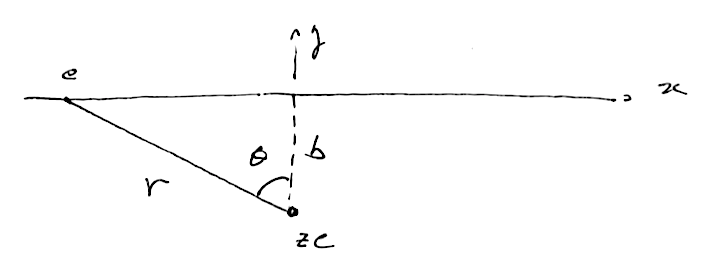
\includegraphics[width=0.5\textwidth]{passRadMat2.png}
  \caption{Illustration of the reference frame in which the particle with mass $M$ is at rest and the atomic electron travels towards it.}
  \label{fig:passRadMat2}
\end{figure}

We can then consider the two main projections of the momentum transfer, where the first is the one along the direction of motion of the electron, i.e. $\Delta\vec{p}$ along the $x$-axis (the direction of motion!) of Fig. \ref{fig:passRadMat2}:

\begin{eqnarray*}
  \Delta p_{\parallel} &=& \int_{-\infty}^{+\infty} \frac{ze^2}{4\pi\epsilon_0}\frac{1}{x^2+b^2}\sin\theta\ dt,\\
                       &=& \int_{-\infty}^{+\infty} \frac{ze^2}{4\pi\epsilon_0}\frac{1}{x^2+b^2}\sin\theta\ \frac{dx}{v},
\end{eqnarray*}
in which we used $dt = dx / v$, and $\theta$ is the angle between the vector $\vec{r}$ and the $y$-axis. Let's assume $v = \text{const}$ and
write
\[\sin\theta = \frac{x}{\sqrt{x^2+ b^2}},\]
so that
\[\Delta p_{\parallel} = \frac{ze^2}{4\pi\epsilon_0v}\int_{-\infty}^{+\infty}\frac{x}{\rr{x^2+b^2}^{\frac{3}{2}}} dx.\]
Now, we use $r = \sqrt{x^2 + b^2}$, with
\begin{eqnarray*}
  \od{r}{x} &=& \frac{1}{2}\frac{2x}{\sqrt{x^2+b^2}}=\frac{x}{r},\\%\frac{x}{\sqrt{x^2+b^2}}\\
  r\,dr &=& x\,dx,
\end{eqnarray*}
from which we get
\begin{eqnarray*}
  \Delta p_{\parallel} &=& \frac{ze^2}{4\pi\epsilon_0v}\int_{-\infty}^{+\infty}\frac{r}{r^3} dr \\&\propto& \int_{-\infty}^{r_0} \frac{1}{r^2}\ dr - \int_{r_0}^{+\infty}\frac{dr}{r^2}\\
             &=& \qq{-\frac{1}{r}}_{-\infty}^{r_0} - \qq{-\frac{1}{r}}_{r_0}^{+\infty} = \qq{-\frac{1}{r}}_{r_0}^{+\infty} - \qq{-\frac{1}{r}}_{r_0}^{+\infty} =0.
\end{eqnarray*}
This shows that the transferred momentum along the x--axis,
i.e. parallel to the direction of the incoming particle, is zero. 

Instead, the component along the $y$-axis, i.e. the orthogonal direction with respect to the direction of motion, can be computed as:
\begin{eqnarray*}
  \Delta p_{\perp} &=& \int_{-\infty}^{+\infty} \frac{ze^2}{4\pi\epsilon_0} \frac{1}{\rr{x^2+b^2}}\cos\theta\frac{dx}{v} \\
             &=&  \frac{ze^2}{4\pi\epsilon_0v} \int_{-\infty}^{+\infty} \frac{1}{b^2}\cos^3\theta dx,
\end{eqnarray*}
in which we used
\[ \cos^2\theta = \frac{b^2}{x^2+b^2}.\]

Now let's compute the integral in $d\theta$:
\begin{eqnarray*}
  x^2 + b^2 &=& \frac{b^2}{\cos^2\theta},\\
  x^2 &=& \frac{b^2\rr{1-\cos^2\theta}}{\cos^2\theta} = b^2\tan^2\theta,\\
  x &=& b\tan\theta,\\
  \od{x}{\theta} &=& \frac{b}{\cos^2\theta},
\end{eqnarray*}
which gives
\begin{eqnarray*}
  \Delta p_{\perp} &=& \frac{ze^2}{4\pi\epsilon_0 vb}\int_{-\frac{\pi}{2}}^{+\frac{\pi}{2}}\cos\theta\ d\theta\\
             &=& \frac{ze^2}{4\pi\epsilon_0 vb} \cdot 2.\\
\end{eqnarray*}
This last equation can simply be written as
\[\Delta p_{\perp} =  \frac{ze^2}{4\pi\epsilon_0 b^2} \cdot \frac{2b}{v}.\]
This means we can see the overall momentum transfer as the momentum transferred by a constant force $ze^2/4\pi\epsilon_0 b^2$ for a time equal to $2b/v$. The "average force" is simply the Coulomb force from a charge $ze$ at a distance equal to the impact parameter, and the time defines the {\bf scattering time}.

An important note at this point is that the trajectory of the electron is assumed essentially to be a straight line, which is clearly an approximation. This approximation holds only in the case where the velocity of the particle of mass $M$ is large enough with respect to the velocity of the electron in its orbit. For this specific calculation we will focus on a very specific energy range of the incident particle: the one where the velocity is large enough to make this approximation valid, but still not too large to break the assumption of a non-relativistic regime.

Since $\Delta p_x = 0$, the only contribution to the energy
transferred to the electron comes from the perpendicular momentum change. In the non-relativistic case, the kinetic energy loss can be written as
\[\Delta E\rr{b} = \frac{\Delta p^2}{2 m_e} = \frac{2z^2e^4}{m_e v^2 \rr{4\pi\epsilon_0}^2b^2},\]
where we highlighted the fact that the energy depends on the impact parameter.
It should be emphasized that the velocity here is non-relativistic in order to be able use the above energy-momentum relation.
While the regime is non-relativistic in this case, we will still express the formula in terms of the velocity normalised to the speed of light $\beta = v/c$: substituting the equation of the classical radius of the electron, the energy loss becomes
\begin{eqnarray*}
  \label{eq:bohr2}
  \Delta E\rr{b} &=& \frac{2z^2e^4}{m_e\beta^2c^2 \rr{4\pi\epsilon_0}^2 b^2}\\
                 &=& \frac{2z^2m_e c^2}{\beta^2 b^2}\qq{\frac{e^2}{4\pi\epsilon_0m_ec^2}}^2\\
                 &=& \frac{2z^2m_e c^2}{\beta^2 b^2}r_e^2.
\end{eqnarray*}

The energy transferred to a single electron of the atom from a particle of mass $M$ and charge $ze$ can thus be written as
\begin{equation}
  \label{eq:bohr3}
 \boxed{ \Delta E = 2m_ec^2\frac{z^2}{\beta^2}\frac{r_e^2}{b^2}.}
\end{equation}

In the reference frame of the interacting particle, the material it encounters can be seen as  a ``beam'' of
electrons moving towards it. The goal is to compute the energy loss per unit path length of the particle: in order to do so, we will express the energy loss as a function of the impact parameter and we will need to start by taking into account all the electrons with a given impact parameter within the ``beam''. 

If $n_e$ is the electron density in
the material (number of electrons per unit volume), then the number of electrons in an element path of the particle $dx$ and with a given impact parameter $b$ will define a cylindrical region around the charge, as shown in Fig. \ref{fig:passRadMat3}, with volume $V$. The number of interacting points with an impact parameter $b\in\qq{b,b+db}$, $dN_I$, will therefore be:
\[dN_I = n_e V = n_e\ 2\pi b\ db dx.\].

\begin{figure}
  \centering 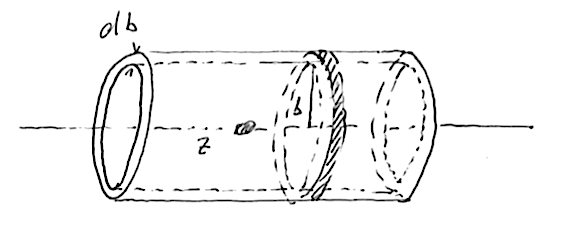
\includegraphics[width=0.5\textwidth]{passRadMat3.png}
  \caption{Illustration of the element cylindrical volume defined for a given impact parameter $b$. }% ,around the charge ze,which volume is given by the formula $2\pi b\ db dx\$ } 
  \label{fig:passRadMat3}
\end{figure}

The absolute value of the element energy loss in the infinitesimal path length $dx$ at a given impact parameter $b$ within an infinitesimal element impact parameter $db$ can then be expressed as follows: 

\[\frac{d^2E}{dxdb} = n_e r_e^2 m_e c^2 \frac{4\pi}{b}
  \frac{z^2}{\beta^2},\]
where we multiplied Eq. \eqref{eq:bohr3} by $dN_I$.
  
In order to compute the energy loss per element path length $dE/dx$, we must integrate the above formula with respect to $b$. This is in principle a clearly divergent integral:
\[\frac{dE}{dx} = n_e r_e^2 m_e c^2 4\pi
  \frac{z^2}{\beta^2} \int_{b_\text{min}}^{b_\text{max}}\frac{db}{b} = n_e r_e^2 m_e c^2 4\pi
  \frac{z^2}{\beta^2} \ln \frac{b_\text{max}}{b_\text{min}} \]
Is it worrisome? No, because the range of possible impact parameters $b$ is necessarily limited. To estimate the energy loss, reasonable estimates of the values of $b_\text{min}$ and $b_\text{max}$ need to be made.

\begin{itemize}
\item The scattering time has to be relatively small as discussed above in order for the electron not to be moving significantly in its atomic orbit during the scattering time. A natural limit in the scattering time will therefore be the revolution period of the electron around the atom, which in the reference frame of the electron is $T_e = 1/\langle \nu_e\rangle$, where 
  $\langle v_e \rangle$ is the average orbital frequency of electrons. As the scattering time could be expressed as approximately $b/v$, then we require that it does not exceed the time needed
  for an electron to complete an orbital revolution. We take into account the time dilation of the revolution period when seen by the moving particle, $\gamma T_e = \gamma /\langle \nu_e\rangle$. As a consequence, $b_\text{max}$ is expressed as 
  \[b_\text{max} = \frac{\gamma v}{\langle v_e \rangle} = \frac{\beta \gamma c}{\langle v_e \rangle}.\]

\item According to the uncertainty principle, 
$$ \Delta p_e  \Delta x > \frac{\hslash}{2}. $$
If the momentum transferred to the electron is equal to the momentum of the electron itself, i.e. $\Delta p_e \sim p_e = m_e \gamma \beta c$, the minimum allowed spatial ``resolution'' $\Delta x$ for the electron position can be taken as $\Delta x = b_\text{min}$, i.e.
  \[b_\text{min} \sim \frac{\hslash}{p_e} = \frac{\hslash}{m_e\beta\gamma c}.\]
\end{itemize}

Having defined the bounds for the integration, the density of electrons in a material can be defined assuming an isotropic material with density $\rho$ [g/cm$^3$], atomic mass $A$ [g/mol$^{-1}$] and atomic number $Z$ [$\#e^-$/atom] using the Number of Avogadro $\mathcal{N}_A$ [mol$^{-1}$] as:
\[n_e = \frac{\mathcal{N}_A Z \rho}{A} \; \; {[\#e^-/\si{cm^{3}}]},\] 
and finally we get
\begin{eqnarray*}
  \od{E}{x} &=& \int_{b_{\min}}^{b_{\max}} 4\pi n_e r_e^2m_e c^2\frac{z^2}{\beta^2}\frac{db}{b}\\
             &=& 4\pi  \frac{\mathcal{N}_A Z \rho}{A} r_e^2m_e c^2\frac{z^2}{\beta^2}\qq{\ln\frac{b_{\max}}{b_{\min}}},\\
\end{eqnarray*}
which gives the expression for Bohr's formula of energy loss of a charged particle traveling in a material:
\begin{equation}
 \boxed{ \der{E}{x} = 4\pi r_e^2m_ec^2\,\frac{\mathcal{N}_A Z\rho}{A}\,\frac{z^2}{\beta^2}\,\ln\frac{m_ec^2\beta^2\gamma^2}{\hslash\langle v_e\rangle }.}
\end{equation}

This approximate estimate of the energy loss of a charged particle in a material has a quite limited kinematic range. A more extended formulation is given in the following section: it will be interesting to note that the two formulations are surprisingly close.

\subsection{The Bethe-Bloch formula}
A more general expression of the energy loss, which is valid also in the relativistic regime and which takes into account more intricate quantum effects has been derived in 1930 by Hans Bethe in the non relativistic regime and then deriving a relativistic correction in 1932. The equation was later completed by Felix Bloch in 1933, who introduced a specific additional term. 

While Bohr's approach was fully classical, Bethe took an quantum-mechanical approach which he extended in the relativistic regime. While a full derivation is beyond the scope of these lectures, we will introduce the Bethe equation from the relation between the energy loss and the impact parameter obtained  from energy-momentum dispersion relation, Eq.~\eqref{eq:bohr3}, yielding
\[ \frac{\Delta E_\text{max}}{\Delta E_\text{min}} =  \frac{b_\text{max}^2}{b_\text{min}^2}.\]
Here it should be noted that the maximal energy transfer will correspond to the minimal impact parameter and vice-versa,  i.e. that \(\Delta E_{max} \propto 1/b_{min}^2\) and \(\Delta E_{min} \propto 1/b_{max}^2\), thus giving the expression above.

The absolute value of energy loss can be expressed in terms of the ratios of the square-root of the maximum and minimal energy losses, which will translate to the logarithm of the ratio divided by $2$: 

\[\frac{dE}{dx} = \frac{\mathcal{N}_A Z \rho}{A} r_e^2 m_e c^2 4\pi
  \frac{z^2}{\beta^2} \frac{1}{2} \log \frac{\Delta E_{max}}{\Delta E_{min}}. \]

We will start from the maximal energy transfer $\Delta E_\text{max}$ from a kinematic standpoint and just consider a two-body scattering of the particle with mass $M$ and charge $ze$ on the electron, which is initially at rest, and compute the maximum kinetic-energy transfer. Let
$\vec{p}$ and $\vec{p}_1$ be, respectively, the momentum of the
particle before and after the scattering, and $\vec{p}_2$ the electron
momentum in the final state, as shown in Fig.~\ref{fig:passRadMat4}.

\begin{figure}
  \centering 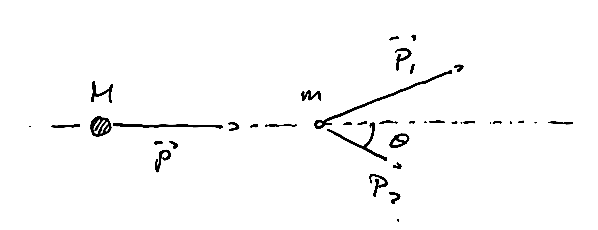
\includegraphics[width=0.5\textwidth]{passRadMat4.png}
  \caption{Illustration of the scattering of a particle with mass $M$ on an electron at rest, used for the computation of the maximum energy loss of the particle (i.e. the maximum kinetic-energy transfer to the electron). The angle $\theta$ is the angle between the momentum of the electron after the scattering and the original direction of the incoming particle.}
  \label{fig:passRadMat4}
\end{figure}

Momentum and energy conservation laws can be written as:
\begin{eqnarray*}
  \vec{p} &=& \vec{p}_1 + \vec{p_2},\\
  E + mc^2 &=& E_1 + E_2.\\
\end{eqnarray*}
From this last equation, using $E^2 = M^2c^4 + p^2 c^2$ and
$p = M \gamma \beta c$:
\begin{eqnarray*}
  E_1 &=& E + mc^2 - E_2,\\
  \qq{M^2c^4 + \vec{p}_1^2c^2}^{\frac{1}{2}} &=& E + mc^2 - E_2,\\
  M^2c^4 + \rr{\vec{p}-\vec{p_2}}^2c^2 &=& \rr{E + mc^2 - E_2}^2,\\
  M^2c^4 + p^2c^2 + p_2^2c^2 -2pp_2c^2\cos\theta &=& E^2 +m^2c^4 +E_2^2\\
      & & +2Emc^2 -2 E_2mc^2 -2EE_2,\\
  -2pp_2c^2\cos\theta &=& 2m^2c^4 +2Emc^2 -2 E_2mc^2 -2EE_2\\
      &=& 2mc^2\rr{mc^2 + E} -2E_2\rr{mc^2 + E}\\
      &=& 2\rr{mc^2 -E_2}\rr{mc^2 + E}.
\end{eqnarray*}
Squaring both terms gives:
\begin{eqnarray*}
  \rr{mc^2+E}^2\rr{E_2^2 + m^2c^4 -2E_2mc^2} &=& p^2p_2^2c^4\cos^2\theta,\\
  \rr{mc^2+E}^2\rr{E_2^2 + m^2c^4 -2E_2mc^2} &=& p^2E_2^2c^4\cos^2\theta - p^2m^2c^6\cos^2\theta.\\
\end{eqnarray*}
Then,
\begin{eqnarray*}
  \qq{\rr{E + mc^2}^2 -p^2c^2\cos^2\theta}E_2^2 & &\\
  -2mc^2 \rr{E+mc^2}^2E_2 & &\\
  +m^2c^4\qq{\rr{E+mc^2}^2+p^2c^2\cos^2\theta} &=& 0.
\end{eqnarray*}
We want to solve this second-order equation for $E_2$. Let's compute the $\Delta/4$:
\begin{eqnarray*}
  \Delta / 4 &=& m^2c^4\rr{E+mc^2}^4\\
             & & - m^2c^4\qq{\rr{E+mc^2}^2+p^2c^2\cos^2\theta}\qq{\rr{E + mc^2}^2 -p^2c^2\cos^2\theta}\\
             &=& m^2c^4p^4c^4\cos^4\theta,\\
  \sqrt{\Delta/4} &=& mc^2 p^2c^2 \cos^2\theta = mc^4 p^2 \cos^2\theta.
\end{eqnarray*}
We finally get to
\[E_2 = mc^2\frac{\rr{E+mc^2}^2 + p^2c^2\cos^2\theta}{\rr{E+mc^2}^2 -
    p^2c^2\cos^2\theta}.\]
This clearly shows that the maximum amount of energy is transferred
when $\cos\theta = 1$, for which the electron energy is
\begin{eqnarray*}
  E_2^{\max} &=&  mc^2\frac{\rr{E+mc^2}^2 + p^2c^2}{\rr{E+mc^2}^2 - p^2c^2}\\
             &=&  mc^2\qq{\frac{E^2+m^2c^4+2Emc^2 + p^2c^2}{E^2+m^2c^4+2Emc^2 - p^2c^2}}\\
             &=&  mc^2\qq{\frac{M^2c^4+m^2c^4+2Emc^2 + 2p^2c^2}{M^2c^4+m^2c^4+2Emc^2}}\\
             &=&  mc^2\qq{1+\frac{2p^2c^2}{M^2c^4+m^2c^4+2Emc^2}}.\\
\end{eqnarray*}
The maximum kinetic energy that can be transferred to the electron is therefore
\[T^{\max} = E_2^{\max} - mc^2 =
  \frac{2mc^2p^2c^2}{M^2c^4+m^2c^4+2Emc^2},\] and if we use $p = Mc\beta\gamma$
and $E = \gamma M c^2$ we get
\[ \boxed{T^{\max} =
  \frac{2m\beta^2\gamma^2c^2}{1+2\gamma\frac{m}{M}+\rr{\frac{m}{M}}^2}.}\]
An useful approximation of this formula in the limit $2\gamma m \ll M$ will be useful for the complete Bethe-Bloch calculation:
\begin{equation}\label{eq:Tmaxapprox}
    \Delta E_{max} = T^{\max} = 2m\beta^2\gamma^2c^2.
\end{equation} 

In order to compute the minimum energy loss of the incoming particle, the intuitive estimate should be the average ionization energy of the electrons of the atom, $\langle I\rangle$. This quantity is non trivial to estimate and was one of the main contributions from Felix Bloch in 1933, who showed that the mean ionization energy can be simply approximated by the relation 

\[\langle I \rangle \sim (10 \, {\rm eV}) \times Z.\]

A similar approximation can be obtained with the Thomas--Fermi model, where $\langle I\rangle $ can be computed from the average ionization energy of hydrogen atoms,
\[\langle I \rangle \sim Z I_H.\]

From the above formula one obtains a formulation of the average ionization energy which depends only on the atomic number $Z$ in units of the electron rest energy (i.e. its mass),

\[ \boxed{\frac{m_e c^2}{I} \sim \frac{3.6 \cdot 10^4}{Z}.}\]

In order to simplify notation, one usually defines the constant $C$ as
\[C = 4\pi r_e^2 m_e c^2 N_A = 0.31\ \frac{\mega\electronvolt}{\gram\cdot\centi\meter^{-2}},\]
and the energy loss formula can then be written as
\begin{equation}
  \frac{1}{\rho}\od{E}{x} = C\,\frac{Z}{A}\,\frac{z^2}{\beta^2}\,\frac{1}{2}\ln\frac{2m_e\gamma^2\beta^2c^2}{I}.
\end{equation}
One often uses $1/\rho\od{E}{x}$ instead of $\od{E}{x}$, in order to highlight the small dependence of the energy loss on the material.

%which, according to the
%1\textsuperscript{st} equation of \ref{eq:bohr2} allows us to get %an
%estimate for $b_{\min}$:
%\[b_{\min} = \frac{ze^2}{\gamma\beta^2m_ec^2\rr{4\pi\epsilon_0}}\]

In fact, by using
\[\frac{m_ec^2}{\langle I \rangle} \sim \frac{3.6\times10^4}{Z},\]
it becomes clear that the energy loss divided by $\rho$ scales as
\[\frac{dE}{\rho dx} \propto \frac{Z}{A}\ln\frac{\text{const}}{Z},\]
which, apart from the density and a logarithmic dependency on $Z^{-1}$, does not depend strongly on the material. If we ignore the logarithmic dependency we obtain that the energy loss per unit of length divided by the density is independent of the material of the detector.

The result of this calculation is often referred to as the Bethe formula. A more precise empirical model for the average ionization energy is obtained from measurements of the ionization energy normalized to the atomic number $Z$, as shown in Fig.~\ref{fig:passRadMat6}. The measurements show a good agreement with the Bloch prediction, with a significant deviation at low $Z$.

\begin{figure}
  \centering 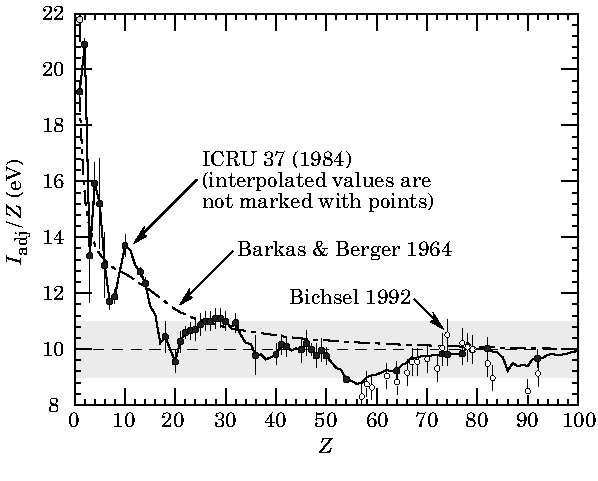
\includegraphics[width=0.75\textwidth]{passRadMat6_Iadj_pegs_adndt}
  \caption{Illustration of the average ionization energy measurement as a function of  the atomic number $Z$. The relation $\langle I \rangle \sim (\SI{10}{eV})\times Z$ is represented by the dashed, horizontal line.}
  \label{fig:passRadMat6}
\end{figure}

A more accurate parameterisation which is valid in a wider range of atomic number \(Z\) is
\begin{eqnarray*}
  \frac{I}{Z} \sim \rr{12 + \frac{Z}{2}}\,\electronvolt &\text{for}& Z \lesssim 10,\\
  \frac{I}{Z} \sim \rr{10 + 60 Z^{-1.2}}\,\electronvolt &\text{for}& Z \gtrsim 10.\\
\end{eqnarray*}

The \(\od{E}{x}\) behaviour described by the Bethe formula is shown in Fig.~\ref{fig:passRadMat8}.

\begin{figure}
  \centering 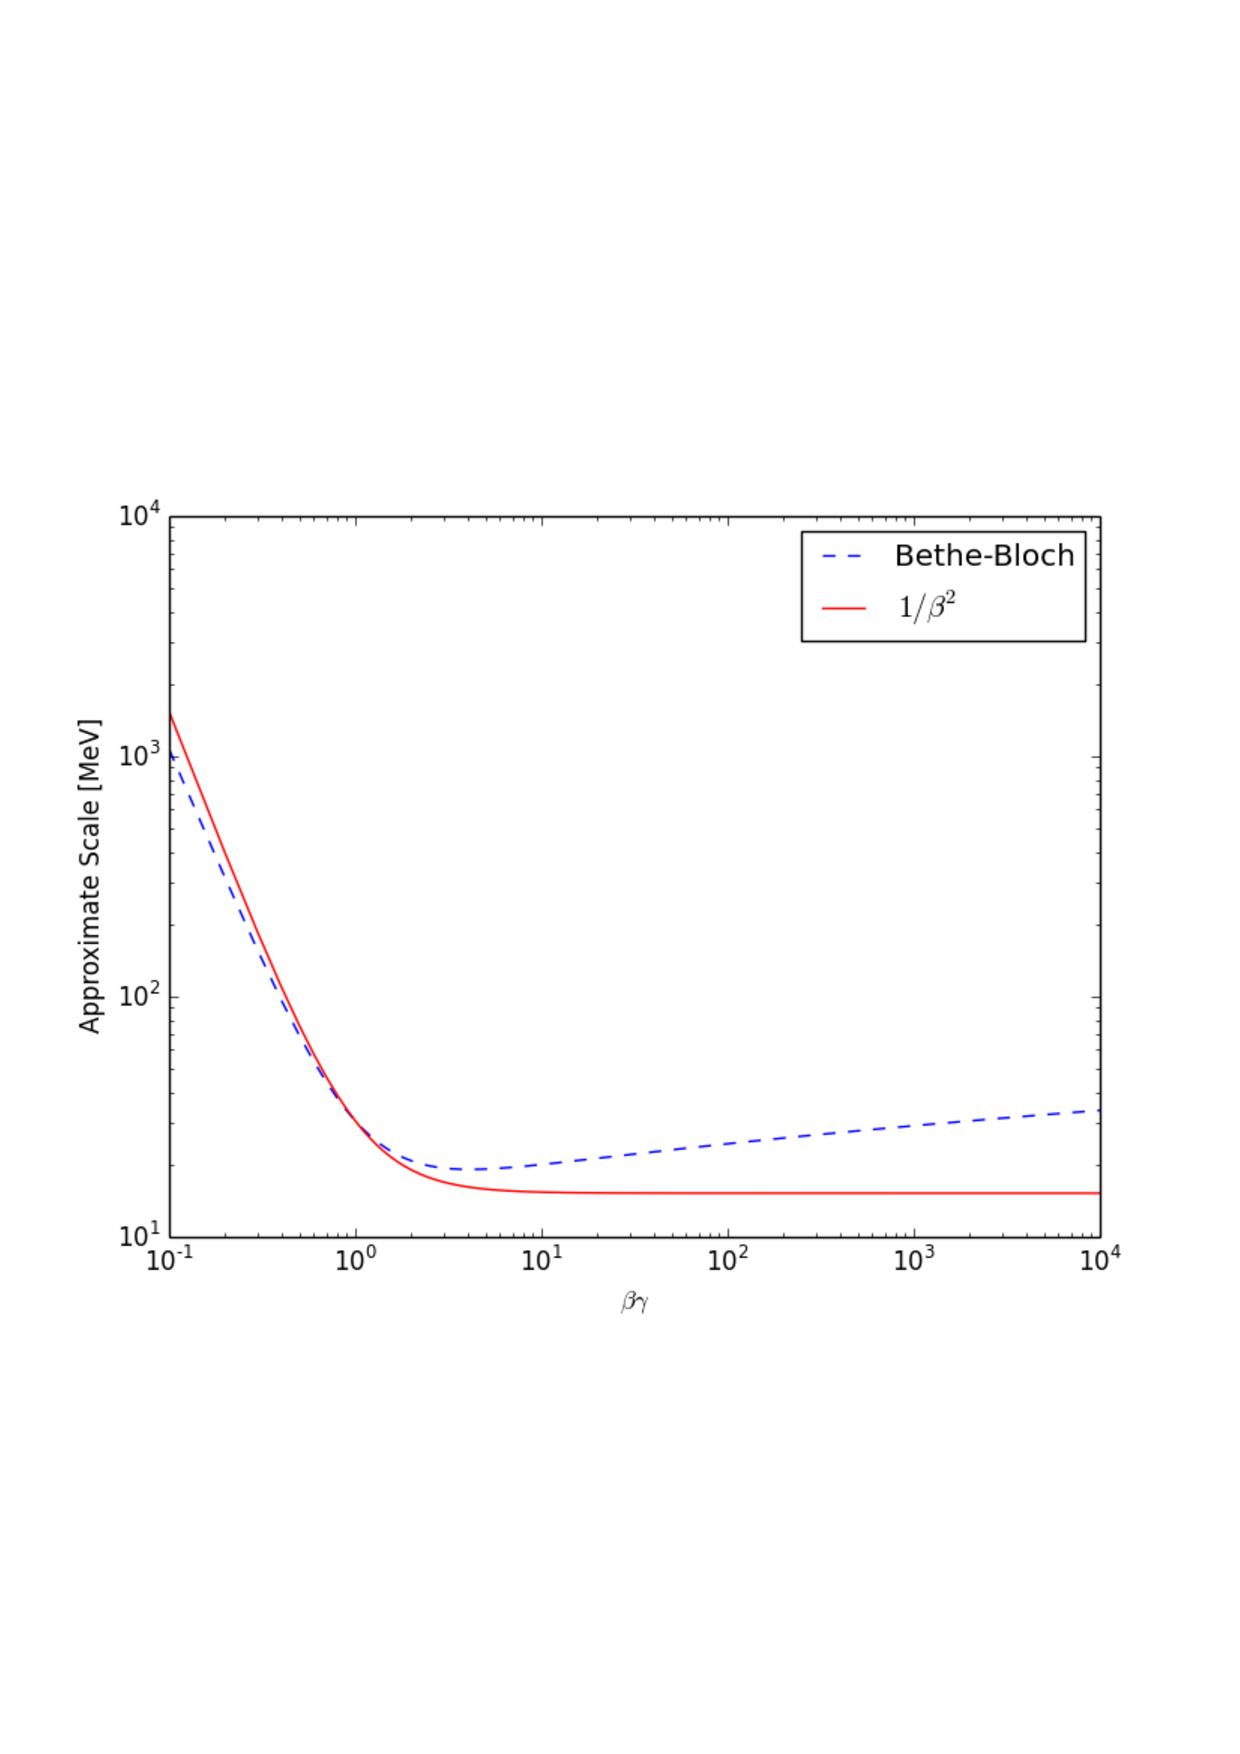
\includegraphics[width=0.75\textwidth]{BetheBloch}
  \caption{Illustration of the behaviour of the energy loss \(\od{E}{x}\) described by the Bethe formula as a function of $\beta \gamma$.}
  \label{fig:passRadMat8}
\end{figure}

\subsubsection{Interpretation}

It is interesting to compare the Bethe formula with the simple dependence in $1/\beta^2$. This shows that in the low energy regime the dominant term  essentially goes as  $1/\beta^2$, indicating that slow particles will lose much more energy by ionization than faster particles. With respect to the simple $1/\beta^2$ behaviour, the Bethe formula shows a slow increase in ionization energy at relativistic velocities, often referred to as \emph{relativistic increase}.

In the higher energy range, compared with the $1/\beta^2$ analytic form, there is a logarithm rise of the energy loss which is interpreted as the increase of the energy loss due to the increase in the electrostatic field "seen" by the probe particle when it is boosted. The electric field components which are orthogonal to the boost axis will be increased by a factor $\gamma$, while the longitudinal component is unchanged.

However, this formulation of the energy loss is incomplete. A more accurate and up-to-date version of the Bethe formula, the Bethe-Bloch formula, is discussed in the next section.

\begin{figure}
  \centering 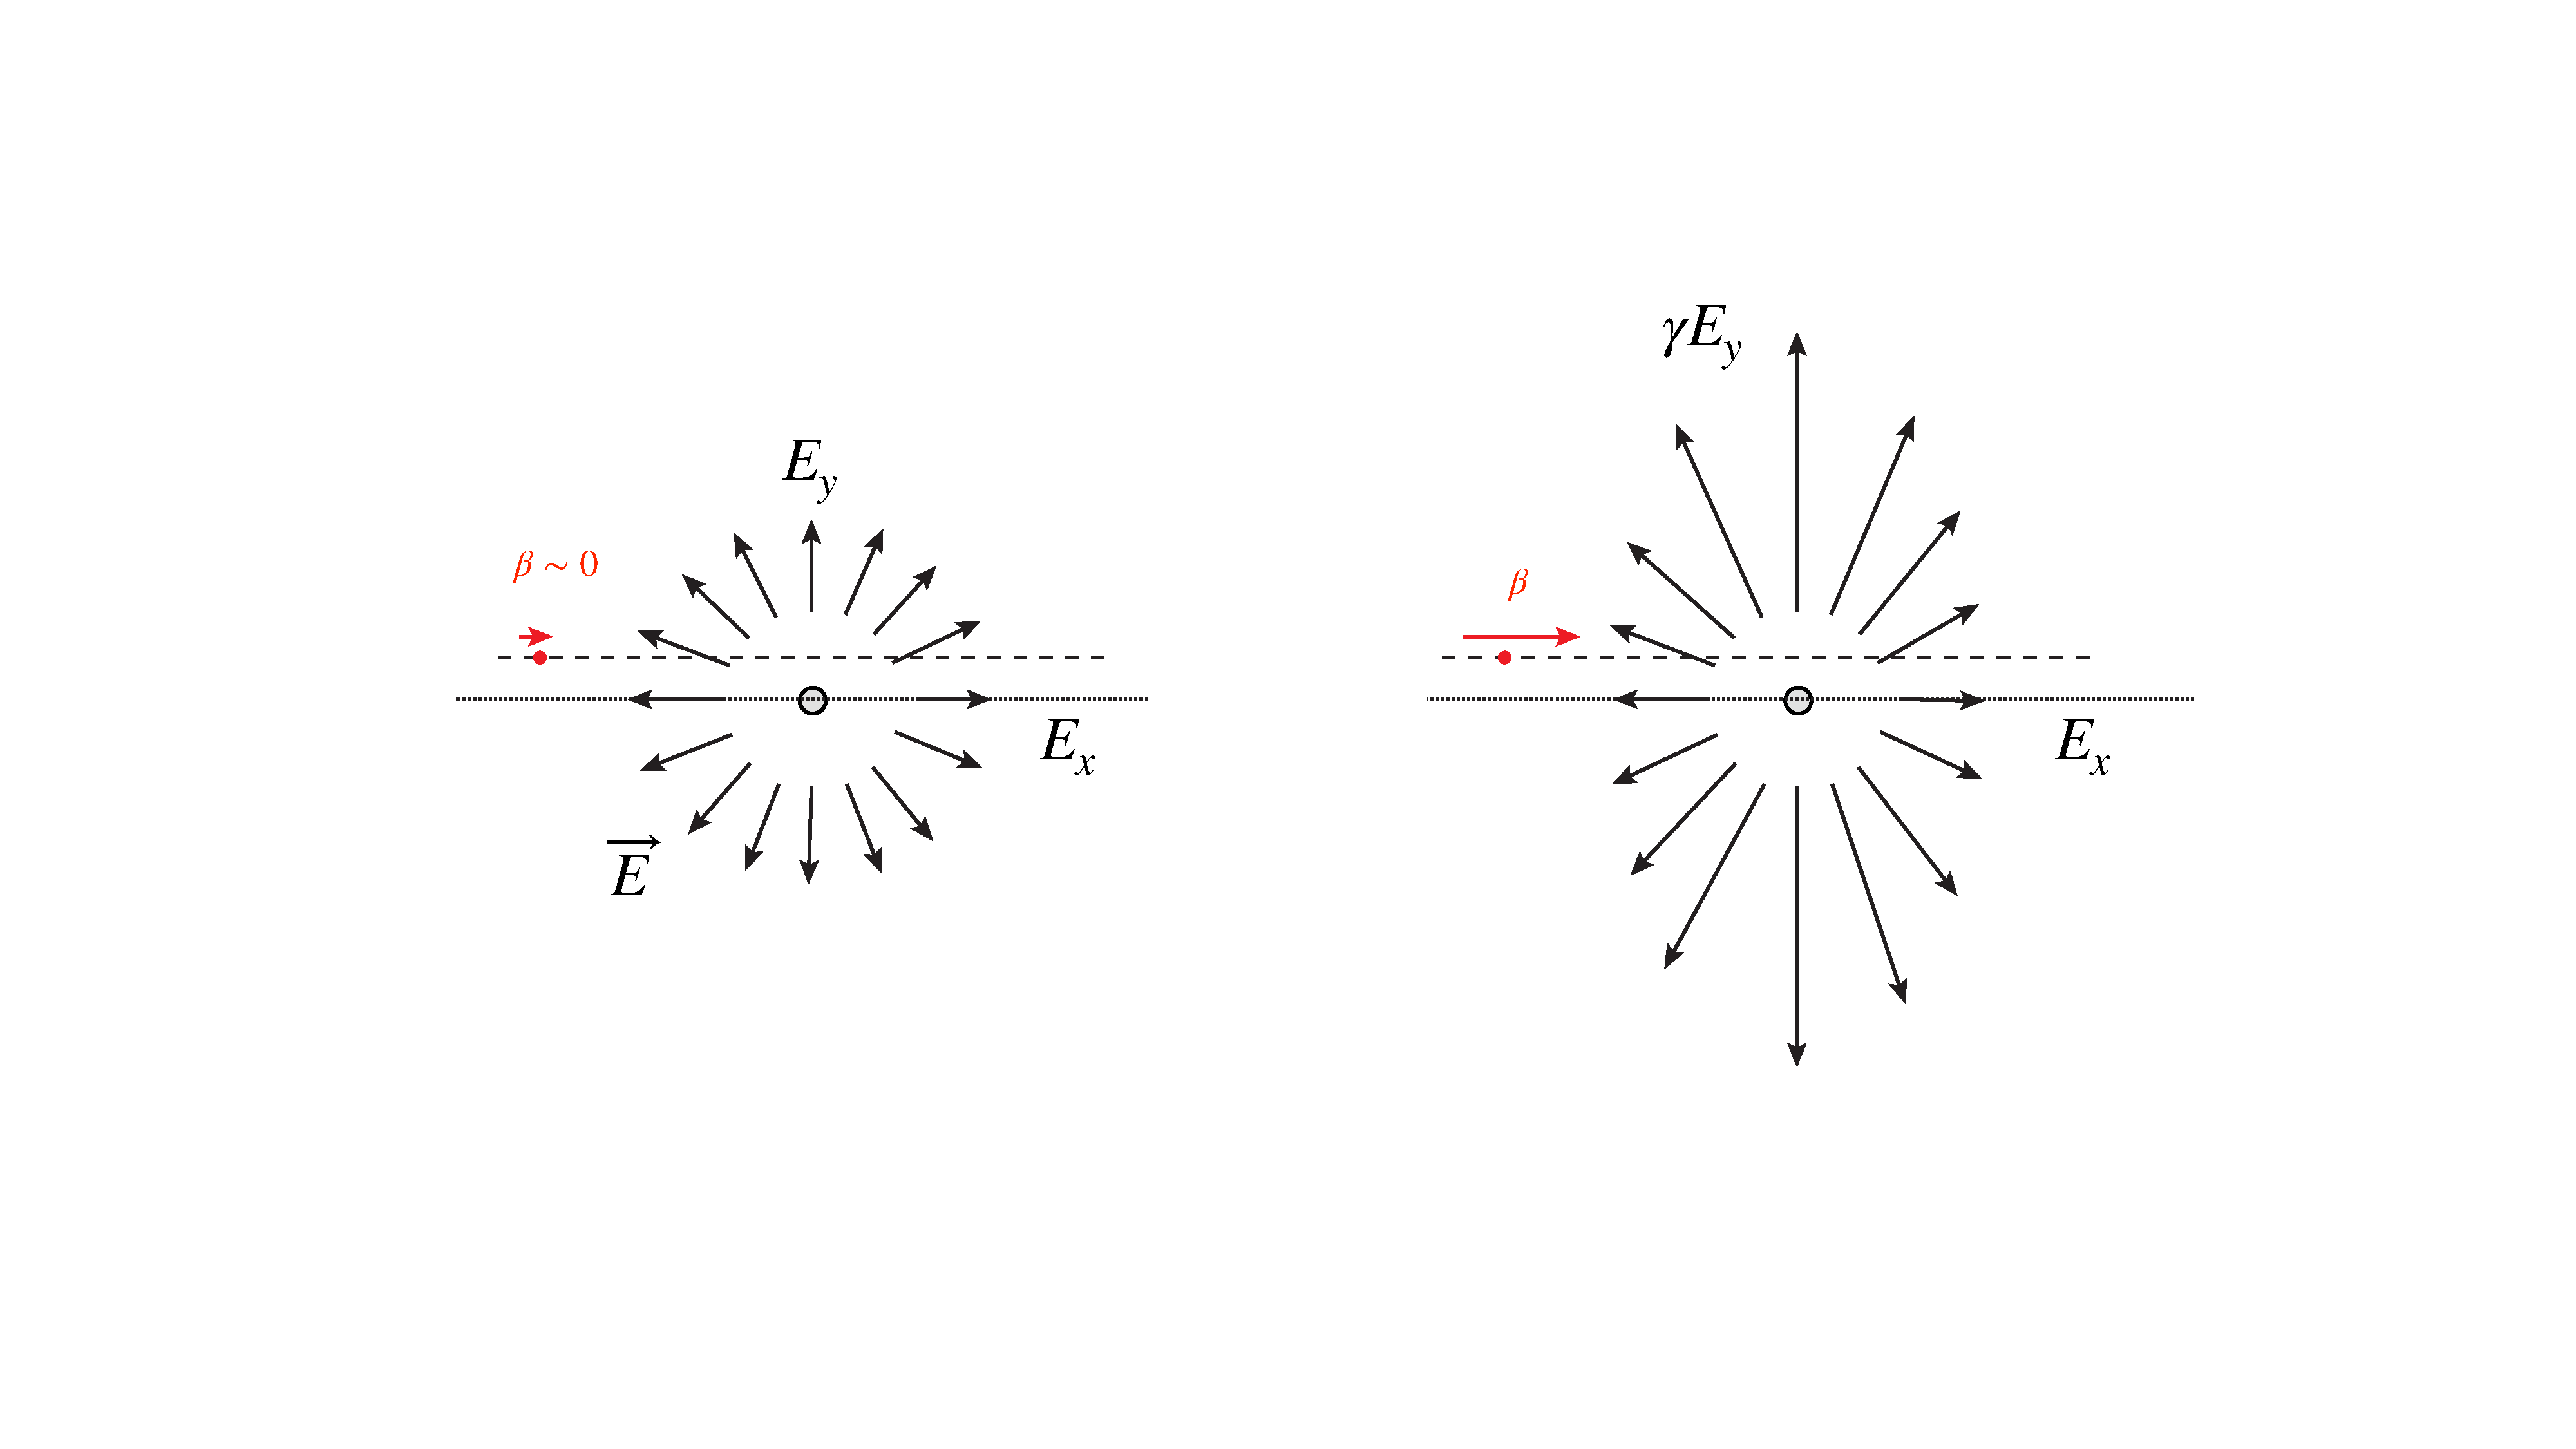
\includegraphics[width=0.8\textwidth]{Field}
  \caption{Illustration of the interpretation of the logarithmic relativistic rise of the energy loss due to the increase of the electric field "seen" by a boosted probe particle.}
  \label{fig:FieldBetheBloch}
\end{figure}


\subsection{The complete Bethe-Bloch formula}
\label{sec:BB} 
The complete Bethe-Bloch formula for the calculation of the energy loss by ionisation, which is valid also in the relativistic regime and takes all known intricate effects into account, is the following:
\[\frac{1}{\rho}\od{E}{x} = Cz^2
  \frac{Z}{A}\frac{1}{\beta^2}\qq{\frac{1}{2}\ln\frac{2m_ec^2\beta^2\gamma^2T_{\max}}{I^2}
    - \beta^2 -\frac{\delta}{2} - \frac{K}{Z}}.\] 
Here $T_{\max}$ corresponds to the maximum kinetic energy which can be transferred to the electrons, as calculated in the previous section. i.e. 
\[T_{\max} = \frac{2m_ec^2\beta^2\gamma^2}{1+2\gamma\frac{m_e}{M} +
    \rr{\frac{m_e}{M}}^2} \xrightarrow{\gamma m_e \ll M}
  2m_ec^2\beta^2\gamma^2,\]and $\delta$ is a term due to the
\emph{density effect} due to the screening of polarisation, which limits the logarithmic growth of
$\od{E}{x}$. The term $K/Z$ is a term which lowers the energy loss for
slowly-moving particles, for which $v$ (and then the kinetic energy
$K$) is not much greater than the electron velocity.\\

\begin{figure}
  \centering 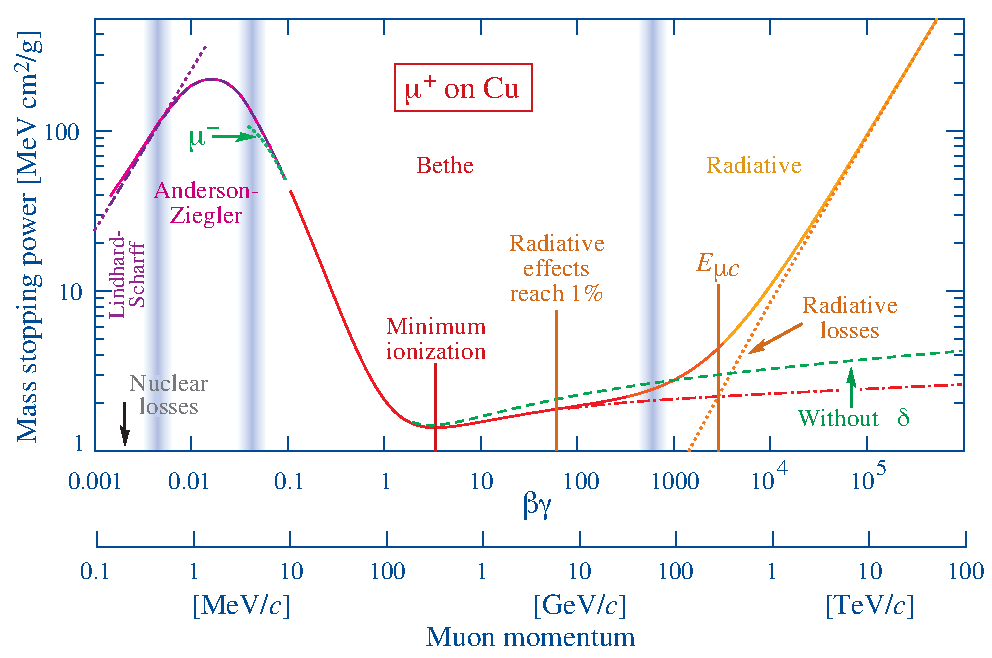
\includegraphics[width=\textwidth]{passRadMat5_rpp_icru49_cu_col}
  \caption{Energy loss normalised to the density of the material ("mass stopping power"), $dE/\rho dx$, for a muon, a particle with a mass of $105 \; \mega\electronvolt$, as a function of its $\beta \gamma$.}
  \label{fig:passRadMat5}
\end{figure}

Figure \ref{fig:passRadMat5} shows on the y--axis the $dE/\rho dx$ of a muon\footnote{Standard model particles will be introduced later in these notes. Here you should consider the muon as a particle identical to the electron, but with a mass of $105 \mega\electronvolt$.} as a function of its momentum. Let's take a look to the region labelled as ``Bethe'' (in which the precision of the formula is around 1\%):
\begin{itemize}
\item at low $\beta$, i.e. at low momentum, the energy loss is dominated by the dependence on $1/\beta^2$;
\item the energy loss has a minimum: particles which are crossing a material such that their energy loss is in this minimum are called \emph{minimally-ionising particles} (MIP); the minimum position is usually at $\beta\gamma \sim 3\div3.5$;
\item after the minimum, the energy loss begins to grow as $2\ln(\beta\gamma)$;
\item in the lowest $\beta\gamma$ region the model is not valid, and empirical models are used to describe the energy loss;
\item in the low $\beta\gamma$ region, the correction $K/Z$ becomes important;
\item for high $\beta\gamma$, the model is no more valid, as the energy loss is dominated by \emph{bremsstrahlung} (described later in this chapter).
\end{itemize}

The correction introduced by $\delta$ is mostly effective at high energy. As the energy of the particle increases, its electric field becomes more flattened and extended, but the real media become polarized, truncating this part of logarithmic rise.

\begin{figure}
  \centering \includegraphics[width=\textwidth]{passRadMat7_dedx_min_06}
  \caption{Value of the energy loss at its minimum (normalised to the  density of the material, $dE/\rho dx$) as a function of the atomic number of different elements ($Z$).
  A linear empirical regression shows that  $dE/\rho dx$ depends on $\ln (Z)$ with a good approximation. }
  \label{fig:passRadMat7}
\end{figure}

Figure \ref{fig:passRadMat7} shows the energy loss at its minimum for different elements. 

Different particles traveling in the same material lose their energy in a similar way. In this case, the Bethe-Bloch law can be seen as
\[-\frac{dE}{dx} = z^2 f(\beta),\]
where $z^2$ multiplies a function of the velocity which is unique for the material.

Since $T=(\gamma-1) Mc^2$, the velocity is a function of $T/M$. This suggests that if the energy loss for a particle with mass $M$ and charge $z$ is known, the energy loss of another particle with mass $M_2$ and $z^2$ will be
\[-\od{E_2}{x} = -\frac{z_2^2}{z_1^2} \od{E_1}{x}\rr{T_2\frac{M_1}{M_2}}.\]

\subsection{Cross Section, Range, Straggling and the Landau Distribution} 
\subsubsection{Cross section}
Equation \ref{eq:bohr3} shows the dependency of $\Delta E$ on the impact parameter $b$. We can compute the cross section of the ionisation energy loss starting from the inverse formula. Let us call $\tilde{E} = \Delta E$ to simplify notation: we have
\[b^2 = \frac{2r_e^2 z^2 m_e c^2}{\beta^2\tilde{E}},\]
and differentiating both members we have
\[|2bdb| = 2r_e^2\,\frac{z^2m_ec^2}{\beta^2}\frac{d\tilde{E}}{\tilde{E}^2},\]
from which we can compute the infinitesimal cross-section in an element cylinder as
\begin{eqnarray*}
  d\sigma &=& \rr{2\pi b} db\\
          &=&2\pi r_e^2 m_e c^2 %n_e
          \frac{z^2}{\beta^2}\frac{d\tilde{E}}{\tilde{E}^2},
\end{eqnarray*}
and finally get the differential cross-section
\[\der{\sigma}{\tilde{E}} = 2\pi r_e^2 m_e c^2 \frac{z^2}{\beta^2}\frac{1}{\tilde{E^2}}.\]
The more energy is lost by the particle, the more collisions are rare.

\subsubsection{Residual Range}
The residual range $R$ is defined as the mean path crossed by a particle in a certain material before losing its entire kinetic energy; it is of course a function of the energy of the particle. Using \(f(E) = -\od{E}{x}\), we have
\begin{eqnarray*}
  R(E) &=& \int_0^R dx \\
       &=& -\int_E^0 \frac{dE}{f(E)}\\
       &=& \int_0^E \frac{dE}{f(E)}.
\end{eqnarray*}
One should note that this quantity is an average quanity: since the energy loss is a stochastic effect, the actual value of $R$ will vary in a certain interval.

In order to measure the residual range it is possible to take an absorber of different length and material and measure the transmission power (ratio of incoming and outgoing particles). Stochastic effects (straggling) are responsible for the smoothed curve of transmission power, as shown in figure \ref{fig:passRadMat8}.

\begin{figure}
  \centering \includegraphics[width=0.6\textwidth]{passRadMat8}
  \caption{Transmission power (fraction of particles in a beam which are transmitted) as a function of the distance traveled by the beam in a given material. Stochastic effects (``straggling'') are responsible for the smoothed curve.
  Note that the average distribution becomes a Gaussian which parameters will be described in Sec. \ref{sec:energystraggling}.
  }
  \label{fig:passRadMat8}
\end{figure}

In order to take into account the effects at low energy loss, it is common to introduce a term like
\[R(E) = R_0(E_{\min}) + \int_{E_{\min}}^E \frac{dE}{f(E)}, \]
which can be measured experimentally, while the integral is computed numerically. Figure \ref{fig:passRadMat9} shows the range divided by $M$ for different particles in different materials. The precision of this prediction is around $1\%$.
\begin{figure}
  \centering \includegraphics[width=\textwidth]{passRadMat9}
  \caption{Range (times density) of ionizing charged particles ($x \rho$) in liquid  hydrogen, helium gas, carbon, iron, and lead. As an example, for a $K^+$ with mass $\SI{493.7}{MeV/c^2}$ and with momentum \SI{700}{MeV/c}, i.e. $\beta \gamma = 1.42$, from the curves one can read $R/M\sim396$, and so the range is $\SI{195}{g cm^{-2}}$.}
  \label{fig:passRadMat9}
\end{figure}


\subsubsection{Channeling}
Channeling is another limit of Bethe-Bloch formula. If a particle crosses a material at a certain critical angle it is possible that it starts to follow a path in which the number of encountered electrons is lower than  average. This is usually happening at a small angle $\theta_{\text{crit}} \sim 1^\circ$ and $\beta \simeq 0.1$, becoming smaller as the energy rises. Figure \ref{fig:passRadMat10} shows an example of this path.

\begin{figure}
  \centering \includegraphics[width=0.5\textwidth]{passRadMat10}
  \caption{Illustration of the phenomenon of channelling, as observed for example in crystals.
  It defines a limit of Bethe Bloch formula.}
  \label{fig:passRadMat10}
\end{figure}

\subsubsection{Energy straggling}\label{sec:energystraggling}
The Bethe-Bloch formula gives an expression of the \emph{average} energy
loss. Since the nature of these interactions is stochastic, the energy
lost by a particle should also be considered as a random variable with a certain distribution.

Although the computation of the energy loss distribution in a material
of length $x$ is difficult (and usually dealt with computer simulation), we will see the limits of very thin and
very thick material.\\

For a \emph{thick material}, we can assume that the energy lost in a single
collision, $\Delta$, is much smaller than the energy of the incoming particle. If
we also assume that this $\Delta$ is small enough  not to change the
$\beta$ of the particle, the central limit theorem ensures us that the
distribution of energy lost by the particle will be Gaussian,
\[f(\Delta) \propto e^{-\frac{\rr{\Delta -
        \bar{\Delta}}^2}{2\sigma^2}},\]
whose expectation value and standard deviation we wish to calculate.
        
The number of collisions in a
length $dl$ with transferred energy
$\tilde{E}\in\qq{\tilde{E},\tilde{E}+d\tilde{E}}$ is
\begin{eqnarray*}
  f(\tilde{E})d\tilde{E} dl &=& \frac{N_A Z \rho}{A} dl \frac{d\sigma}{d\tilde{E}}d\tilde{E}\\
                            &=& \frac{N_A Z\rho}{A} 2\pi r_e^2 m_e c^2 \frac{z^2}{\beta^2}\frac{d\tilde{E}}{\tilde{E}^2}dl\\
                            &=& \frac{C}{2}\frac{Z\rho}{A}\frac{z^2}{\beta^2}\frac{d\tilde{E}}{\tilde{E}^2}dl.
\end{eqnarray*}
If we assume that $\beta$ is constant and neglect the $K/Z$ and density effect corrections, the integral of the Bethe-Bloch
can be easily computed,
\[\int_0^x \frac{dE}{\rho dx} dx = C
  \frac{Z}{A}\frac{z^2}{\beta^2}\frac{1}{2}\rr{\ln\frac{2m_ec^2\beta^2\gamma^2}{I}
    -\beta^2}x,\]
which gives $\bar\Delta$,
\[\bar\Delta = \xi\rr{\ln\frac{2m_ec^2\beta^2\gamma^2}{I} - \beta^2},\]
where we used
\[\xi = \frac{C}{2}\frac{Z}{A}\frac{z^2}{\beta^2}x.\]

The variance can be obtained from its definition:
\begin{eqnarray*}
  \sigma^2 &=& \int f(\tilde{E})\tilde{E}^2d\tilde{E}dl\\
           &=& \int d\tilde{E} dl \frac{C}{2} \frac{Z\rho}{A}\frac{z^2}{\beta^2}\\
           &=&  \frac{C}{2} \frac{Z\rho}{A}\frac{z^2}{\beta^2} \rr{E^{\max} - E^{\min}}x\\
           &\simeq&  \frac{C}{2} \frac{Z\rho}{A}\frac{z^2}{\beta^2}T^{\max}x\\
           &=&  \frac{C}{2} \frac{Z\rho}{A}\frac{z^2}{\beta^2}2m_ec^2\beta^2\gamma^2 x\\
           &=&  C\frac{Z\rho}{A}z^2m_ec^2\gamma^2 x,\\
\end{eqnarray*}
where we replaced $T^{\max}$ with its approximation for $2\gamma m<<M$ from Eq. \eqref{eq:Tmaxapprox}. \\

For a \emph{thin material} we cannot apply the central limit theorem: the
Gaussian approximation will fail, as interactions between particles are rare. In this case, the fluctuations in the energy loss will follow the Landau distribution with a most probable value $\Delta_p < \bar\Delta$:
\[f(\lambda) = \frac{1}{\sqrt{2\pi}} e^{-\frac{\rr{\lambda + e^{-\lambda}}}{2}},\]
where
\[ \lambda = \frac{\Delta - \Delta_p}{\xi}.\]
Other laws which are describing different regions exists. An example of straggling function is shown in Fig. \ref{fig:passRadMat11}.
\begin{figure}
  \centering \includegraphics[width=\textwidth]{passRadMat11}
  \caption{Illustration of the Landau distribution modelling the energy loss $\Delta$ over a small distance $x$ travelled by \SI{500}{MeV} pions in silicon.}
  \label{fig:passRadMat11}
\end{figure}


\subsection{Interpretation and Particle Identification} 
As shown in figure \ref{fig:passRadMat12} the energy loss at its minimum is around $1\div2\, \mega\electronvolt\,\gram^{-1}\centi\meter^2$. This corresponds, for a medium with $\rho \sim 10\, \gram\centi\meter^{-3}$ like copper, to a mean energy loss per $1\,\centi\meter$ of \SI{16}{MeV}, i.e. a non--negligible amount of energy.


\begin{figure}
  \centering \includegraphics[width=\textwidth]{passRadMat12}
  \caption{Energy loss as a function of $\beta \gamma$, illustrating the relatively small variations of the position in $\beta \gamma$ of the minimum of ionization, and that curves are very similar. The correspondence in terms of momentum with $\beta \gamma$ for different particles is also given.}
  \label{fig:passRadMat12}
\end{figure}

Since the energy loss reaches its maximum for low $\beta$, if the absorber is deep enough, the maximum amount of released energy will be close to the stopping point of the particle.

The dependence of Bethe-Bloch formula on the incoming particle mass and charge allows, as shown in figure \ref{fig:passRadMat13}, the identification of different kind of particles. This property has been crucial in the past, allowing classification and discovery of elementary particles.

\begin{figure}
  \centering \includegraphics[width=\textwidth]{passRadMat13}
  \caption{The measured energy loss from different particles as a function of their momentum, illustrating the discriminating power of the ionization energy loss measurements -- combined with  momentum measurements -- to identify particles.}
  \label{fig:passRadMat13}
\end{figure}
%%% Local Variables:
%%% mode: latex
%%% TeX-master: "../book"
%%% End:

\subsection{Orders of magnitude} 
The Bethe-Bloch formula allows us to answer a fundamental experimental question: why do \(\alpha\), \(\beta\) and \(\gamma\) radiation travel with so different ranges in matter? We will use Fig.~\ref{fig:passRadMat12} to provide a quantitative answer.

We know that \(\alpha\) particles are helium nuclei, i.e. their mass is \(m_\alpha\approx4m_p=\SI{3.7}{GeV}\) and their charge is $+2e$. The typical energy -- \emph{kinetic} energy -- of \(\alpha\) particles is of a few \si{MeV}. As the \(\alpha\) particle is relatively heavy, \SI{5}{MeV} of kinetic energy correspond for example to
\[\beta\gamma = \frac{pc}{mc^2} = \frac{\sqrt{(T+mc^2)^2-(mc^2)^2}}{mc^2} = \frac{\sqrt{T^2+2mc^2T}}{mc^2} \approx 0.05.\]
An $\alpha$ particle will therefore be in the part of the Bethe Bloch formula in which the energy loss is high; its charge is twice as much as the electron charge, which brings  a factor four higher energy loss. Depending on the material, its energy loss normalised to the material density will be of about \SI{8}{MeV/gcm^2}, which leads to a range of a few \si{cm} in air, and about \SI{20}{\micro m} in water. This is consistent with the experimental evidence for which \(\alpha\) radiation can be easily stopped with a thin paper layer.

In the case of $\beta^-$ and $\beta^+$ radiation, i.e. electrons and positrons with $m_e=\SI{511}{keV}$, the typical energies depend on the decaying nucleus and are between a few \si{keV} to about \SI{1}{MeV}. An electron with \SI{500}{keV} of kinetic energy from \(^{40}K\) decays will for example have \(\beta\gamma\approx2\), close to the minimally ionising particle regime; while an electron with \SI{100}{keV} from \(^{60}Co\) decays will have \(\beta\gamma\approx0.7\), with almost a factor \(3\) higher energy loss per \si{cm}.
Experimentally, a thin aluminium foil is usually enough to absorb $\beta$ radiation.

As for $\gamma$ radiation, i.e. massless photons with energies between a few \si{keV} to a few \si{MeV} (or, in the case of X rays, between about \SI{100}{eV} and a few \si{keV}), the energy loss mechanisms are described in detail in the following sections. One should note that photons can induce ionisation indirectly, via the photoelectric effect and Compton effect. We anticipate that the typical range of $\gamma$ radiation in matter is higher than for $\alpha$ and $\beta$ radiation, and can reach a few \si{km} in air: long, high-density absorbers (e.g. lead) must be used in order to safely stop $\gamma$ radiation.
 
\subsection*{Take-home lessons}
\begin{itemize}
    \item  Charged particles lose their energy, when interacting with matter, due to ionisation or excitation of other atoms, to Coulomb scattering with atomic nuclei or to radiation emission in the field of atomic nuclei (\emph{bremsstrahlung}). Photons instead undergo photoelectric effect, Compton scattering and electron-positron pair production.
    \item The atomic model by Niels Bohr assumes a hydrogen atom to be composed of a proton and an electron, kept together by the Coulomb potential. The mass of the proton is assumed to be much greater than the mass of the electron, and the atom is assumed to be stationary, i.e. electrons revolve in stationary, circular orbits around the nucleus without radiating energy. Angular momentum is conserved and is assumed to be quantised in units of $\hslash$: as a result, the energy and radius of each orbits are quantised (in agreement to the experimental observations). This model is often sufficient to calculate with good accuracy the energy loss of particles interacting with matter.
    \item In Bohr's model, a particle which travels close to an atom with velocity $v$ receives a change in momentum ("momentum transfer") due to the Coulomb interaction between the particle and atomic electrons. The momentum transfer is only in the directional orthogonal to the direction of the particle, and is equivalent to having an  "average force" -- independent on time -- applied at a distance equal to the impact parameter $b$, for a time $2b/v$ ("scattering time"). This calculation assumes the electron orbit to be a straight line, an assumption which is accurate only when $v$ is significantly larger than the orbital velocity of the electron. One can derive, in the non-relativistic approximation, the energy loss of the incoming particle as a function of its impact parameter. By combining this quantity with the number of electrons along the path of the particle, one can calculate the average energy loss per element path length, $\od{E}{x}$: it is however necessary to know the minimum and maximum impact parameter values of the particle. The minimum value can be taken from the indetermination principle as the $b_\text{min}=\Delta x \approx \hslash/p_e$, where $p_e$ is the momentum of the electron; the maximum value can instead be taken from the fact that the scattering time should be less than the period of the electron orbit, and correcting the resulting value for relativistic time dilation effects. As a result, one gets Bohr's formula, which is able to describe energy loss of a particle in a medium with reasonable accuracy over a limited kinematic range.
    \item The Bethe-Bloch formula comes from a more accurate calculation of energy loss, based on a quantum mechanical approach which is also extended in the relativistic regime. Again, the main task is to express the energy transfer as a function of the impact parameter -- the higher the first, the lower the second. The maximum energy transfer depends on the mass of the electron, the mass of the particle and its velocity, and can often be approximated as $\Delta E_\text{max} = 2m\beta^2\gamma^2c^2$. The mimimum energy transfer instead depends on the average ionisation energy of the atom, which is proportional to its atomic number ($\langle I\rangle\propto Z$). The Bethe-Bloch formula is often expressed in terms of the energy loss per unit path length normalised to the density of the material, $\frac{1}{\rho}\od{E}{X}$, which does not depend strongly on the material.
    \item The complete calculation of the Bethe-Bloch energy loss shows three different regimes. When the incoming particle is very slow (low $\beta\gamma$), it loses energy as $1/\beta^2$.  The energy loss $\frac{1}{\rho}\od{E}{X}$ then reaches a minimum for $\beta\gamma\approx3\div3.5$, corresponding to about \SI{2}{MeV g/cm^2} (\emph{minimally ionising particle}). Then, the energy loss rises with $2\ln(\beta\gamma)$, due to the fact that the electic field seen by the incoming particle is increased by the Lorentz boost. For very low $\beta\gamma$ the calculation is not correct, and empirical models must be used; for very high $\beta\gamma$, radiative effects (bremmstrahlung) become dominant and the energy loss from ionisation starts becoming negligible. Two corrections are included, the \emph{density effect} for high $\beta\gamma$ (the electric field is screened due to polarisation of the medium) and the \emph{shell correction} for low $\beta\gamma$ (slow particles aren't much faster than electrons).
    \item The cross-section of the ionisation energy loss can be obtained from the Bethe-Bloch formula, and is inversely proportional to the energy loss: collisions with high energy loss are therefore less probable than those with low energy loss.
    \item The Bethe-Bloch calculation gives the \emph{average} energy loss. Since energy loss is a stochastic process, in real life one needs to take into account the thickness of the material the particle travels in. In thick materials, one can assume that the energy loss is due to a sequence of collisions in which only a small fraction of the energy of the particle is lost: one can therefore apply the central limit theorem and calculate the mean and standard deviation of the distribution of energy loss, when density effect and shell correction are neglected. In the limit of very thin materials, one cannot apply the central limit theorem and fluctuations in the energy loss will follow a Landau distribution, which has a most probable value lower than the average energy loss from the Bethe-Block formula.
    \item The \emph{range} of a particle in a medium is defined as its mean path before it loses all its kinetic energy. Its experimental curve is smeared (due to straggling) with respect to an ideal integration of the energy loss per unit path length.
    \item By comparing the \od{E}{x} of different particles, one may deduce their mass and charge, and \emph{perform particle identification}.
    \item Depending on the angle at which a particle travels in a medium, it may be \emph{channeled} in a path in which the number of encountered electrons is lowered than the average. This phenomenon happens for small incident angles, $\approx \SI{1}{deg}$, and $\beta\approx0.1$.
\end{itemize}
\section*{Questions}
\begin{itemize}
    \item 
\end{itemize}
%\chapter{Interaction of Particles with Matter Part-II - Radiation}
%\label{matter_radiation_interaction} % Always give a unique label

\section{The Cerenkov Radiation}
Let's consider a particle travelling through a medium with a
refraction index $n$ and a velocity $\beta c$. It is possible that the
particle travels at a speed which is higher than the one of the light
in that medium, which is $c/n$, if
\[\beta > \frac{1}{n}.\]
This phenomenon is usually associated with the emission of a radiation
by the material (\emph{Cerenkov radiation}) which is represented in
figure \ref{fig:passRadMat14}\footnote{A nice animation which illustrates the effect is available at  \url{https://upload.wikimedia.org/wikipedia/commons/8/87/Cherenkov_radiation-animation.gif}.}. Atoms of the material are polarised by
the motion of the particle and release radiation in spherical
waves. The envelope of these waves is a plane wave emitted at a
certain angle $\theta_c$. If the distance covered by the light
emission in a time $t$ is equal to the distance covered by the
particle, then
\[\beta c t \cos\theta_c = \frac{ct}{n}\]
which gives:
\[\cos\theta_c = \frac{1}{n\beta}\]

\begin{figure}
  \centering \includegraphics[width=0.5\textwidth]{passRadMat14}
  \caption{Illustration of the Cerenkov Radiation and its emission angle $\theta$.}
  \label{fig:passRadMat14}
\end{figure}

The emitted energy per unit of photon frequency $\omega$ by a particle of charge $ze$
can be computed within classical electrodynamics, and corresponds to
\begin{eqnarray*}
  \frac{d^2E}{dx d\omega} &=& \frac{z^2e^2}{4\pi \epsilon_0}\frac{\omega}{c^2}\qq{1-\frac{1}{\beta^2n^2(\omega)}}  \\
                          &=& z^2\frac{\alpha\hslash\omega}{c}\sin^2(\theta_c(\omega)),
\end{eqnarray*}
where $\alpha=\frac{e^2}{4\pi\epsilon_0\hslash c}=\frac{1}{137}$ is the fine structure constant. 
A typical Cerenkov detector is sensitive (and transparent) only to some part of the photon spectrum. The number of photons with energy equal to $\hslash\omega$ can be written as
\[\frac{d^2n}{dxd\omega}=\frac{z^2\alpha}{c}\sin^2\theta_c(\omega),\]
and we want to integrate it in an interval of visible frequencies. We obtain
\begin{eqnarray*}
  \frac{dn}{dx}&=&\frac{z^2\alpha}{c}\int_{\Delta\omega} \sin^2\theta_c(\omega)d\omega  \\
               &\simeq& \frac{z^2\alpha}{c}\avg{\sin^2\theta_c}\Delta\omega,
\end{eqnarray*}
which for a typical range of photon spectrum $\hslash\omega\approx\SI{2}{eV}$ corresponds to
\[\avg{\der{n}{x}} \sim 700\ \text{photons}\ \centi\meter^{-1} \times
  z^2\sin^2\theta_c\] Cerenkov emission does not contribute to the
energy loss for a particle, since its intensity is $10^{3}$ times less
than ionisation energy loss, this is rather intuitive since this
emission is due to a polarisation effect. Typically, Cerenkov photon
have an energy of $4\,\electronvolt$, and the average energy loss is
around $2\,\kilo\electronvolt$.

\begin{figure}
  \centering \includegraphics[width=\textwidth]{passRadMat15}
  \caption{Top left: Cerenkov ring due to the emission of Cerenkov
    radiation. Bottom: Super Kamiokande is a detector which is
    based on Cerenkov radiation detection, the radiator material is
    water ($50\times10^3 \kilo\gram$) and it is equipped with 11k
    light detectors. Top right: an image of a reconstructed Cerenkov ring produced by a muon in the Super Kamiokande detector.}
  \label{fig:passRadMat15}
\end{figure}


\section{Multiple Scattering}
We have computed the Rutherford differential cross section in Chapter~\ref{Scattering-1}, Eq.~\eqref{eq:rutherford}, which describes the interaction between a particle of charge $z$ and an atomic nucleus with atomic number $Z$, as a function of the scattering angle $\theta$:
\[
 \frac{d\sigma}{d\Omega} =\left( \frac{zZe^2}{16 \pi \varepsilon_0 E_k} \right)^2 \times \frac{1}{\sin^4 \dfrac{\theta}{2}}.
\]
Here we used $E_k$ to denote the kinetic energy of the charged particle.

From the Rutherford formulation it is clear that the cross section diverges at small angles,
\[\lim_{\theta\to 0}\der{\sigma}{\Omega} = \infty. \]
This implies that the average scattering angle is $\avg{\theta} = 0$. 

Under the hypothesis that a particle undergoes multiple independent scatterings in a material, it is reasonable to assume the mean scattering angle to be Gaussian--distributed. How much will the standard deviation (or the variance) of this Gaussian be? This is the relevant experimental quantity, as a beam of particles traveling in matter will somehow be ``spread'' by that amount.

In an element of solid angle $d\Omega = 2\pi \sin \theta d\theta \approx 2 \pi \theta d\theta$, the number of collisions can be expressed then as a function of the kinetic energy, which can be written as $E_k = pv/2$:
\begin{eqnarray*}
  d^2n &=& \frac{\mathcal{N}_A\rho}{A} d\sigma dx\\
  &=& \frac{\mathcal{N}_A\rho}{A} \frac{d\sigma}{d\Omega} 2 \pi \theta d\theta dx\\
  &=& 8\pi \frac{\mathcal{N}_A\rho}{A} r_e^2 z^2Z^2 \frac{(m_ec^2)^2}{p^2v^2}\frac{\theta d\theta dx}{\theta^4},
\end{eqnarray*}
in which we used the complete Rutherford cross section computed in Eq.~\ref{eq:rutherford} in the approximation of small angles.

Given that the average scattering angle is zero, the variance of the scattering angle is simply the expectation value of the square of the scattering angle,
\begin{eqnarray*}
  \theta^2_s &=& \int \theta^2  \frac{d^2n}{d\theta dx}d\theta \\
                   &=& 8\pi r_e^2 \frac{\mathcal{N}_A \rho}{A} z^2 Z^2 \frac{\rr{m_ec^2}^2}{p^2v^2}\int\frac{d\theta}{\theta}\\
                   &=& 8\pi r_e^2 \frac{\mathcal{N}_A \rho}{A} z^2 Z^2 \frac{\rr{m_ec^2}^2}{p^2v^2} \ln\frac{\theta_{\max}}{\theta_{\min}}
\end{eqnarray*}

From here we can use again the relation between the impact parameter $b$ and the scattering angle $\theta$ of Eq.~\eqref{eq:ImpactParameterR} derived in Chapter~\ref{Scattering-1}, which can be written in terms of $r_e$ and replacing $E=1/2 Mv^2$ as
\[\tan\frac{\theta}{2} = zZ\frac{m_ec^2}{Mv^2}\frac{r_e}{b}.\]
For small values of $\theta$, and taking into account the fact that $\theta_{max}$ corresponds to $1/b_{\min}$ and $\theta_{\min}$ corresponds to $1/b_{\max}$, we can write
\[\frac{\theta_{\max}}{\theta_{\min}} \sim \frac{1/b_{\min}}{1/b_{\max}} = \frac{b_{\max}}{b_{\min}}.\]

Now let's find an estimate for $b_{\max}$ and $b_{\min}$. We will assume that the impact parameter must be smaller than the atomic radius in the Thomas--Fermi model, which is given by
\[b_{\max}=\avg{r_{\text{atom}}}\sim\rr{\frac{r_e}{\alpha^2}}Z^{-\frac{1}{3}},\]
and that $b$ must be greater than the radius of the nucleus in the phenomenological model,
\[b_{\min}=\avg{r_{\text{nucl}}}\sim [ 1.3 \, {\rm (fm)} ]  A^{\frac{1}{3}} \sim \frac{r_e }{2} A^{\frac{1}{3}}.\]
We can therefore write
\begin{eqnarray*}
  \frac{b_{\max}}{b_{\min}} &=& \frac{2}{\alpha^2}\rr{\frac{Z}{A}}^{\frac{1}{3}} Z^{-\frac{2}{3}}\\
                            &=& \qq{\frac{\sqrt{2}}{\alpha}\rr{\frac{Z}{A}}^{\frac{1}{6}}Z^{-\frac{1}{3}}}^2\\
  &\sim& \rr{183\,Z^{-\frac{1}{3}}}^2.
\end{eqnarray*}
The expression for $\theta^2_s$, moving the square of the expression above out of the logarithm, becomes
\[\theta^2_s = \rr{\frac{4\pi\rr{m_ec^2}^2}{\alpha}}\rr{\frac{z}{pv}}^2\qq{4r_e^2\alpha \frac{\mathcal{N}_AZ^2\rho}{A}\ln\rr{183 Z^{-\frac{1}{3}}}}\]

To further simplify this expression it is useful
to define the \emph{radiation length} of a material, $X_0$, as
\begin{equation}
\label{eq:x0}
    \frac{1}{X_0} = 4r_e^2\alpha\frac{\mathcal{N}_AZ^2\rho}{A}\ln\rr{183\,Z^{-\frac{1}{3}}},
\end{equation}
and the constant
\[E_s = m_e c^2 \sqrt{\frac{4\pi}{\alpha}} \sim 21\,\mega\electronvolt.\]
We can then compute the last integral over $x$,
\[\avg{\theta^2_s} = \int \theta_s^2 dx,\]
and finally get
\[\sqrt{\avg{\theta^2_s}} = z \frac{E_s}{\rho v}\sqrt{\frac{x}{X_0}}.\]

\section{Radiation in the Nuclear Electrostatic Field}
  
\subsection{Bremsstrahlung}
  
The \emph{Bremsstrahlung} (``braking radiation'' in German) is a radiation emitted when a
particle is decelerated by the electric field generated by a nucleus.

The calculation of the radiation emitted by an electron which moves
across the nuclear field has been done by Bethe and Heitler in 1934
and takes into account effects due to quantum mechanics. The process is written as
\[e^-\ N\to N\ e^-\ \gamma,\]
where the final state photon is emitted in the interaction.

\begin{figure}
  \centering \includegraphics[width=0.6\textwidth]{passRadMat16}
  \caption{Illustration of the scattering of a charged particle by the Coulomb potential of a nucleus. 
  The moving scattered particle has a mass $M$, a charge $ze$ and a velocity $v$, while the nucleus has charge $Ze$ and the scattering angle is denoted as $\theta$; $b$ is the impact parameter. The nucleus produces an electric field which ``brakes'' the particle in motion and deviates its trajectory.
  }
\item{}
  \label{fig:passRadMat16}
\end{figure}

In the reference frame of the particle, the electric field is widened
by a factor $\gamma$ in the transverse direction as illustrated in Figure~\ref{fig:FieldBetheBloch}. Let us
consider a nucleus of charge $Ze$ and an incoming particle with charge
$ze$, mass $M$, velocity $v$ and with an impact parameter $b$ (see
figure \ref{fig:passRadMat16}). At the point of minimum distance the acceleration along the direction of motion vanishes, and the velocity is orthogonal to the particle-nucleus direction. We can write the first principle of dynamics in the reference frame of the moving particle as
\[a' = \frac{\gamma}{M} \frac{zZe^2}{4\pi\epsilon_0 r^2},\] 
where we introduced the $\gamma$ factor as an approximation for the averaged effect of the force on the probe particle in the region where it is closest to the nucleus.

In classical electrodynamics the radiated power is calculated as\footnote{See §14.2 from Ref.~\cite{jackson} - page 664.}
\begin{eqnarray}
\label{eq:AcceleratedChargePower}
  W' &=&  \frac{\rr{ze}^2}{6\pi\epsilon_0} \frac{a'^2}{c^3} \nonumber \\
     &=& \gamma^2 \frac{2}{3} \frac{z^4 Z^2 e^6}{\rr{4\pi\epsilon_0}^3}\frac{1}{r^4 M^2 c^3}.
\end{eqnarray}

The scattering time will then be  equal to
$2r/\gamma v$, which is the time during which the particle (in its rest frame) "feels" effectively the Coulomb potential and therefore the time is shorten by the length contraction due to the velocity of the nucleus in the probe particle's rest frame. The  energy emitted during this time $2r/\gamma v$ can then be calculated as
\begin{eqnarray*}
  \Delta E' &=& \int W' dt' \\
            &=& \gamma \frac{4}{3} \frac{z^4 Z^2 e^6}{\rr{4\pi\epsilon_0}^3} \frac{1}{r^3 M^2 c^3 v}.
\end{eqnarray*}

The frequency of this phenomenon is $\omega'_c = \gamma v/2r$, and so the emission frequency spectrum is
\[\frac{dE'}{d\omega'} \sim \frac{\Delta E'}{\omega'_c} = \frac{8}{3}
  \frac{z^4Z^2e^6}{\rr{4\pi\epsilon_0}^3}\frac{1}{r^2 M^2 c^3 v^2}\]
Since energy and frequency are linked by a constant, the frequency
spectrum is Lorentz--invariant. (The same argument does not apply for
the angle of emission of the radiation, but in the relativistic limit
the bremsstrahlung is emitted at $\theta \simeq 0$ and is independent
on the frequency.) This allows us to use the same formula in the
laboratory reference frame, which can be written in terms of the classical electron radius $r_e$ and of the fine structure constant $\alpha$ as
\[\frac{dE}{d\omega} = \frac{8}{3}r_e^2
  \frac{z^4Z^2e^2}{4\pi\epsilon_0}\frac{m_e^2}{M^2}\frac{1}{r^2
    \beta^2 c} = \frac{8}{3}r_e^2
  z^4Z^2(\hslash\alpha)\frac{m_e^2}{M^2}\frac{1}{r^2
    \beta^2}.\]
Energy is radiated as photons, and we can calculate the number of radiated photons  with energy $E_{\gamma}$:
since $E_\gamma = \hslash \omega$, one has
\[ dn (E_{\gamma}) = \frac{1}{E_\gamma} dE(E_\gamma),\]
which can be written in terms of energy spectrum $\der{E}{E_{\gamma}}$ as follows (be careful: this should not be seen as a simple derivative, but is the spectrum in bins of energies that is divided by the emitted energy to get the number of emitted photons):
\[ \der{n (E_{\gamma}) }{E_{\gamma}} = \frac{1}{E_\gamma} \der{E}{\hslash \omega}. \]

We want to calculate the number of radiated photons per unit of length of the path of the particle. Similarly to the case of Fig.~\ref{fig:passRadMat3}, we first need to evaluate the number of targets (i.e. nuclei) at reach for a given impact parameter $b\in\qq{b,b+db}$ and per unit of length $dl$, which is given by
\[\frac{\mathcal{N}_A\rho}{A} 2\pi b\,db\,dl.\]
From this, we get
\[\frac{d^2n}{dE_\gamma dl} = \frac{1}{E_\gamma}\frac{16\pi}{3} \frac{z^4}{\beta^2}r_e^2 \alpha \frac{m_e^2}{M^2} \frac{\mathcal{N}_AZ^2\rho}{A} \frac{b\ db}{r^2}.\]
If we assume that the distance at which the interaction takes place is $r = b$, we can integrate over $b$ and obtain
\[\frac{d^2n}{dE_\gamma dl} = \frac{1}{E_\gamma}\frac{16\pi}{3} \frac{z^4}{\beta^2}r_e^2 \alpha \frac{m_e^2}{M^2} \frac{\mathcal{N}_AZ^2\rho}{A} \ln\frac{b_{\max}}{b_{\min}}\]
In order to integrate this term over the photon energy, many non--trivial effects should be taken in consideration - in particular the shielding effect of the electrons in the atom.

As it was done for the energy loss by ionization, it is useful to define the energy loss in terms of the normalized path length $x$, where
\[x = \rho l\]
is expressed in \(\si{g/cm^2}\). The energy released by bremsstrahlung per unit length will then be
\[\frac{dE}{dx} = \int_0^E \frac{d^2n}{dE_\gamma dx} E_\gamma dE_\gamma.\]
In principle the energy is dependent on the impact parameter:  however, in this simplified (approximated) approach we will assume that the energy and the impact parameter are independent. As in the case of multiple scattering, one can take as integration limits for the impact parameter the approximated expression of the size of the nucleus and the size of the atom as a function of the atomic number, and obtain
\[\der{E}{x} = \frac{z^4}{\beta^2} \frac{m_e^2}{M^2}4r_e^2\alpha \frac{\mathcal{N}_AZ^2}{A}\ln\rr{183\ Z^{-\frac{1}{3}}}E\]

\subsection{Bremstrahlung for electrons}
For an {\bf electron} ($M = m_e$ and $z=1$), which in typical nuclear and particle physics experiments is a relativistic particle ($\beta \sim 1$), the energy loss can be expressed in terms of the radiation length $X_0$ defined in Eq.~\ref{eq:x0} as
\[\frac{dE}{dx} \simeq \frac{E}{X_0}.\]
A more detailed computation,which takes into account the phenomenon of screening from the atomic electrons,  gives
\[\der{E}{x} = 4r_e^2\alpha \frac{\mathcal{N}_AZ^2}{A}\qq{\ln\rr{183\ Z^{-\frac{1}{3}}}+\frac{1}{18}}E.\]

\subsection{Critical Energy}
The \emph{critical energy} for a given particle in a material is the value of energy for which the energy loss by radiation equals the energy loss by  ionization.
For the electron, an empiric parameterisation of the critical energy is given by
\[ E_c=\frac{800}{Z+1.2} \si{MeV}.\]

\subsection{Interpretation and summary}
The radiated power via bremsstrahlung is proportional to the square of the acceleration, i.e. to the inverse square of the mass (because the Coulomb potential does not depend on the particle mass). Consequently, this phenomenon is more important for very light particles (the electron and its antiparticle, the positron), while for particles of higher mass the effect is appreciable only at high energies: this is illustrated by Fig. \ref{fig:passRadMat17}, which shows the energy loss by bremsstrahlung and ionisation for electrons and positrons. Above a  few $\mega\electronvolt$ the bremsstrahlung process dominates over ionisation: the energy threshold at which this happens is called \emph{critical energy}, and depends on the material.

We have seen that the energy loss is almost constant (if expressed as a function of the particle energy). This is not completely true because the bremsstrahlung scales with energy!

From Fig. \ref{fig:passRadMat17} one can also see how the ionisation term (which dominates at low energy) is different for electrons and positrons, as expected (the material is not made of anti--matter!). Other effects are present at low energies:
\begin{itemize}
\item M\o{}ller scattering: $e^-\ e^- \to e^-\ e^-$;
\item Bhabha scattering:  $e^+\ e^- \to e^+\ e^-$;
\item Positron annihilation in matter: $e^+\ e^- \to \gamma \ \gamma $.
\end{itemize}
  
\begin{figure}
  \centering \includegraphics[width=\textwidth]{passRadMat17}
  \caption{Energy loss by bremsstrahlung and ionisation for electrons and positrons in a lead ($Z=82$) target, as a function of their energy. One can see how the ionisation term (which dominates at low energy) is different for electrons and positrons.
  The critical energy for electrons in typical materials is $\sim 10\,\mega\electronvolt$.
  Additional effects which give minor contributions to the energy loss (M\o{}ller scattering, Bhabha scattering and positron annihilation) are also shown.}
\item{}
  \label{fig:passRadMat17}
\end{figure}

\section{Interactions of Photons in Matter}\label{sec:IntPhotonsMatter}
\subsection{Photoelectric effect}
For photons with energy between the ionisation energy for the material and E$\sim 100\,\kilo\electronvolt$ the dominant interaction is photoelectric effect.

The interaction happens between a photon and an electron which is still bound to the atom. A similar interaction between a free electron and a photon can not happen due to the conservation of energy and momentum. In fact, if we denote the photon and electron energy and momentum as $E$, $E_e$ and $\vec{p}$, $\vec{p_e}$, respectively  (see Fig. \ref{fig:passRadMat18}), the conservation of the four-momentum norm can be written as
\begin{figure}
  \centering \includegraphics[width=0.5\textwidth]{passRadMat18}
  \caption{Illustration of the interaction between a photon and an atomic electron and the photoelectric effect. This simple diagram cannot take place alone due to energy and momentum conservation: what really happens is that the photon interacts with the atom as a whole.}
\item{}
  \label{fig:passRadMat18}
\end{figure}

\begin{eqnarray*}
  \rr{E+m,\vec{p}}^2 &=& \rr{E_e, \vec{p_e}}^2,\\
  E^2 + m^2 +2Em -p^2 &=& m^2,\\
  Em &=& 0,
\end{eqnarray*}
which is impossible.

The complete reaction for photoelectric effect is therefore
\[\gamma\ A \to A^+\ e^-.\]
If $E_l$ is the binding energy of the atom, electrons are emitted with energy
\[T = E_\gamma - E_l.\]
The cross section for this process is very small at high energy and grows when the photon energy approaches the binding energy of the $K$, $L$, $M\dots$ shells. Calculating the cross section of this process is hard, because the wave functions of the atomic electrons are complex to write -- although, for photon energies above the binding energy of the $K$ shell it's mostly $K$ electrons which contribute. For $E_\gamma \ll m_e c^2$ the cross section can be approximated as
\[\sigma_{\text{ph}} \simeq k Z^5 \frac{1}{E_\gamma^3},\]
where $k$ is a constant which depends only on $r_e$, $\alpha$ and $m_ec^2$, i.e. does not depend on the material.

\begin{figure}
  \centering \includegraphics[width=\textwidth]{passRadMat17-5}
  \caption{Left: cross section of the photoelectric effect as a function of the photon energy $E_\gamma$. We can observe some peak near the energy of levels, which are due to the fact that electrons from more and more external shells start contributing when the photon energy is high enough. \\ Right: total photon interaction cross section as a function of $E_\gamma$ (bold line), with the individual contributions from photoelectric effect, Compton scattering and pair production.}
\item{}
  \label{fig:passRadMat17-5}
\end{figure}


\subsection{Compton effect}
When the photon energy is much greater than the binding energy of the electron, one can neglect the binding energy of the latter and consider atomic electrons as free particles. In this case, the dominant interaction is Compton scattering,
\[\gamma\ e^- \to \gamma\ e^-.\]

Let's compute the energy of the scattered photon, $E'$, in the reference frame of the initial electron of mass $m$, which is at rest (see figure \ref{fig:passRadMat19}).\\
\begin{figure}
  \centering \includegraphics[width=0.5\textwidth]{passRadMat19}
  \caption{Illustration of the Compton effect: $\gamma$ is the photon with energy $h\nu$, $e$ is the electron at rest.
  After the collision the two particles scatter and in the picture we identify the scattering angle as $\theta$, i.e. the angle between the photon direction in the initial and final state. }
\item{}
  \label{fig:passRadMat19}
\end{figure}
We will use natural units in order to simplify notation, and denote with the subscript $e$ the electron quantities in the final state. The conservation of energy requires
\[E+m = E' + E_e,\]
while the conservation of momentum can be written as
\begin{eqnarray*}
  \vec{p} &=& \vec{p}'+\vec{p_e},\\
  \vec{p_e} &=& \vec{p} - \vec{p}'.
\end{eqnarray*}
We are interested in the photon energy in the final state, so we square the electron momentum with the goal of reducing the system of equations to one unknown:
\[p_e^2 = p^2 + p'^2 -2pp'\cos\theta,\]
while the energy-momentum equation for the electron can be written as
\[p_e^2 = E_e - m^2.\]
We use $E_e = E-E'+m$ and get
\begin{eqnarray*}
  \rr{E-E'+m}^2-m^2 &=& p^2 + p'^2 -2 pp'\cos\theta,\\
  2Em -2EE' -2E'm &=& -2EE'\cos\theta,\\
  E'\rr{E+m-E\cos\theta} &=& Em,
\end{eqnarray*}
which can be written as
\[E' = \frac{mE}{m+E-E\cos\theta}.\]
Finally, if we define $\epsilon = E/m$, we can write the photon energy in the final state as
\[E' = \frac{E}{1+\epsilon\rr{1-\cos\theta}}.\]
In agreement with intuition, the photon energy will be maximum for $\cos\theta = 1$ and minimum for $\cos\theta = -1$.

The energy released by the electron is
\begin{eqnarray*}
  \Delta E &=&  E-E'\\
           &=& h\nu - h\nu'\\
  &=& h\nu - \frac{h\nu}{1+\epsilon\rr{1-\cos\theta}}\\
  &=& \frac{h\nu\qq{1+\epsilon\rr{1-\cos\theta}}-h\nu}{1+\epsilon\rr{1-\cos\theta}},\\
  \Delta E &=& \frac{\epsilon h \nu \rr{1-\cos\theta}}{1+\epsilon\rr{1-\cos\theta}}.
\end{eqnarray*}
The maximum released energy corresponds to the minimum of $E'$, precisely:
\[\Delta E^{\max} = \frac{2 h \nu \epsilon}{1+2\epsilon} = h\nu \frac{2\epsilon}{1+2\epsilon}.\]
Reintroducing $c$, we come to the expression
\[\Delta E^{\max} = \frac{2\epsilon^2 m c^2}{1+2\epsilon},\]
which is called the \emph{Compton edge}.

The differential cross section for Compton scattering has been computed in 1928 by Klein and Nishina using quantum electrodynamics, and can be written as
\[\der{\sigma}{\Omega} = \frac{1}{2} r_e^2 \frac{Z}{A}\frac{E'}{E}\qq{1+\rr{\frac{E'}{E}}^2 + \rr{\frac{E'}{E}}\sin^2\theta}.\]
Keep in mind that the photon energy in the final state depends on the original photon energy and from the scattering angle, $E' = E'\rr{E,\theta}$. From this differential cross section one can compute (in a non-trivial way!) the high-energy limit of the total cross section for $E_\gamma\gg m_ec^2$,
\[\sigma_{\text{Compton}} \sim h\frac{Z}{A} \frac{8\pi r_e^2}{3}\frac{1}{E_\gamma},\]
and the low energy limit,
\[\sigma_{\text{Compton}} \sim h\frac{Z}{A} \frac{8\pi r_e^2}{3}\rr{1-2\frac{E_\gamma}{m_ec^2}}.\]

\begin{figure}
  \centering \includegraphics[width=0.5\textwidth]{passRadMat20}
  \caption{Distribution of the energy of electrons from Compton scattering, which illustrates the dependence of the Compton edge on the energy $h\nu$ of the incident photon. }
\item{}
  \label{fig:passRadMat20}
\end{figure}

\subsection{Classical Processes}
Two additional processes give minor contributions to the interaction of photons with matter, Thomson and Rayleigh scattering, which can be calculated using classical electrodynamics alone.

Thomson scattering corresponds to the electron--photon scattering when electrons can be considered as free and the photon energy is $E_\gamma \ll m_ec^2$. In this case the process, is modeled as an atomic electron which oscillates under the presence of an electromagnetic wave, emitting a secondary spherical wave.
The cross section for Thomson scattering is the following:
\[\sigma = Z\frac{8\pi}{3} r_e^2\]
and corresponds to the low energy limit of the Klein--Nishina formula.

In Rayleigh scattering, the whole atom takes part to the elastic scattering as a single object. For this reason this process is also called \emph{coherent scattering}.

While these two classical processes are important in atomic physics, they can be neglected when considering high-energy physics experiments, where usually -- for $E_\gamma\lesssim 2m_ec^2$ -- one takes into account only the photoelectric and Compton effects.

\subsection{Electron-Positron pair creation}
The creation of an electron--positron pair from a single photon would be
impossible in vacuum, because of four-momentum conservation. In order to
allow the process of \emph{pair production} by a photon, an external
electric field is needed. Of course, this process can happen in
presence of a nucleus (``recoil on a nucleus''),
\[\gamma\ N \to e^+\ e^-\ N,\]
or of another particle, like an atomic electron (``recoil on an electron''),
\[\gamma\ e^- \to e^+\ e^-\ e^-.\]
\begin{figure}
  \centering \includegraphics[width=0.5\textwidth]{passRadMat21}
  \caption{Illustration of the creation of an electron--positron pair in the presence of a nucleus $N$.}
\item{}
  \label{fig:passRadMat21}
\end{figure}

Pair production can only happen when the photon energy is above
$2m_ec^2$ (when the recoil is on a nucleus) or above $4m_ec^2$ (when the recoil is on an electron). In this second case the cross section is lower (see
Fig. \ref{fig:passRadMat22}).
\begin{figure}
  \centering \includegraphics[width=\textwidth]{passRadMat22}
  \caption{Photon differential interaction cross sections in (a) carbon ($Z=6$) and (b) lead ($Z=82$), as a function of the probe photon energy. The agreement between the data and the prediction is clearly visible. The contributions to pair production in the presence of a nucleus or of an electron are denoted as $\kappa_\text{nuc}$ and $\kappa_e$, respectively.
  }
\item{}
  \label{fig:passRadMat22}
\end{figure}

As in the case of bremsstrahlung, pair production is screened at high energy,
which happens usually when $2m_ec^2 \ll E_\gamma \ll m_ec^2Z^{-1/3}/\alpha$. In this case, one has
\[\sigma_{\text{pair}} = \frac{Z^2}{137}r_e^2\rr{\frac{28}{9}\ln\frac{2E_\gamma}{m_ec^2}-\frac{218}{27}}.\]
When $E_\gamma \gg m_ec^2Z^{-1/3}/\alpha$, instead, the nucleus is screened and one has
\[\sigma_{\text{pair}} = \frac{Z^2}{137}r_e^2\rr{\frac{28}{9}\ln\frac{183}{Z^{\frac{1}{3}}}-\frac{2}{27}}.\]
Above the two--electron threshold the cross section rises sharply and when the nucleus appears to be screened it becomes constant.

At high energy one has
\[\sigma \propto Z,\]
and one can write
\[\sigma \sim \frac{7}{9} \frac{1}{X_0}\frac{A}{\mathcal{N}_A}\]
%It is important to notice the constant factor $\frac{7}{9}$ which will be found again in the calculation of mean free path.

\section{Electromagnetic showers}\label{sec:passRadMat_emShowers}
When they travel in a material, electrons and positrons  whose energy is above the critical energy (for electrons/positrons) of that material, or photons  whose energy is above the pair production  threshold, can start a cascade process which leads to the production of many electrons/positrons/photons in the material. This process is called \emph{electromagnetic shower} and is at the basis of the detection of these particles, with particle detectors called \emph{calorimeters}.\\

A schematic of this process is shown in Fig.
\ref{fig:passRadMat23}. Bremsstrahlung and pair production are the two
effects which dominate at high (electron/positron/photon) energy. A simplified model assumes that for
each travelled $X_0$, each photon converts into an electron--positron pair and
each electron/positron radiates a photon via bremsstrahlung. Under this approximation the
electromagnetic shower grows up, as long as the particle energy remains above the critical energy (as the pair
production threshold is usually lower than the critical energy).  Since the number of particles
doubles after one $X_0$, the number of particle after a distance $x$
(measured in terms of radiation lengths of the material, $X_0$) is
\[N = 2^x.\]
At each step, the energy held by the particle gets divided by
$2$, so one has
\[E_{N} = \frac{E_0}{2^x}.\]

Here are some values for the critical energy in different materials:

\begin{table}[h!]
\centering
  \begin{tabular}{ll}
    \hline
    Material & $E_c$                     \\ \hline
    Pb       & $5.5\  \mega\electronvolt$ \\
    Cu       & $24.8\  \mega\electronvolt$ \\
    Fe       & $27.4\  \mega\electronvolt$ \\
    Al       & $51.0\  \mega\electronvolt$ \\ \hline
  \end{tabular}
\end{table}

The maximum number of particles in the shower is reached after a
certain distance $x_{\max}$, for which the mean kinetic energy of the
particles will be equal to the critical energy,
\[\avg{E} = E_c \sim \frac{E}{2^x},\]
which gives
\[x_{\max}=\frac{\ln{\frac{E}{E_c}}}{\ln2}.\] For example, in the case of an electron of
$100\,\giga\electronvolt$, the maximum number of particles will be
reached for $x_{\max} \sim 13 X_0$, which for lead 
($X_0 \simeq 0.6\,\centi\meter$) corresponds to
$\sim 10\,\centi\meter$.

\begin{figure}
  \centering \includegraphics[width=0.6\textwidth]{passRadMat23}
  \caption{Schematic view of an electromagnetic shower.
  Here $X_0$ indicates the length of each interaction which causes a loss of energy, due to the splitting described in the text. The process ends (and the shower ``stops'') when the particle energy reaches $E<E_c$.}
  \label{fig:passRadMat23}
\end{figure}


\subsubsection{Hadronic showers}
High energy hadrons usually interact with matter through nuclear processes, with a much lower cross section than electromagnetic interactions.
\begin{figure}
  \centering \includegraphics[width=0.4\textwidth]{calo4}
  \caption{}
\item{}
  \label{fig:calo4}
\end{figure}

For hadrons above few $\giga\electronvolt$, the nuclear inelastic cross section does not depend on which hadron is interaction or its energy and it's usually parameterized as:
\[\sigma_{\text{inel}} = \sigma_0 A^{0.7},\qquad \sigma_0 \sim 35\,\milli\barn\]


Elastic interaction are present, but do not contribute to the number of particles and are not considered in the production of hadronic showers, on the other hand, there are many different inelastic process from which many hadrons can be produced, developing hadronic showers.

Nuclear processes which leads to hadronic showers can be classified as:
\begin{itemize}
\item Intra--nuclear showers, in which the nucleus produces hadrons
  \item Inter--nuclear showers, in which secondary particles produced in the collisions interact with other nuclei.
\end{itemize}
The main inelastic process which contribute are:
\begin{itemize}
\item \textbf{Spallation}, in which a collision between two nuclei produces a large number of secondary hadrons. This is the most probable process;
\item \textbf{Nuclear evaporation}, where an excited nucleus undergoes a transition to a stable state releasing hadrons;
  \item \textbf{Nuclear fission}, induced by the capture of slow neutrons from a nucleus (see REF TBA) or after spallation.
\end{itemize}

\begin{figure}
  \centering \includegraphics[width=0.9\textwidth]{calo5}
  \caption{Top: Inter--nuclear cascade with spallation. Bottom left: nuclear evaporation. Bottom right: Nuclear fission.}
\item{}
  \label{fig:calo5}
\end{figure}


Among the particles produced in these interaction there are $\pi^0$, which decay immediately in two photons, which starts their electromagnetic shower. Typically the electromagnetic fraction of an hadronic shower (composed of $\gamma$, $e^\pm$, $\pi^0$ and $\eta^0$) is around
\[f_{EM} \sim 30\,\%\]
Also part of the energy is not transferred to the detector material:
\begin{itemize}
\item some nucleus can absorb energy and move to an higher stable state;
\item minimum ionising muons can be produced;
\item neutral stable (or quasi--stable) particles can be produced (neutrinos, $K^0_L$ or neutrons);
\end{itemize}
the detectable part of a shower, via the ionisation of $p$, $\pi$, $K^\pm$, represent $\sim 40\,\%$ of the energy. Since a great fraction of the initial energy can not be detected, hadronic calorimeters have a much lower resolution than e.m. ones.

As analogy to the radiation length $X_0$, it is possible to define the mean hadronic interaction length $\lambda_a$. As shown in section REF TBA, the mean free path for hadronic interaction can be expressed as:
\[\avg{x} = \lambda = \frac{1}{\mu}\]
where $\mu$ is defined as:
\[\mu = \sigma \frac{N_T}{V} = \sigma n_T\]
where $\sigma$ is the inelastic cross section, $N_T$ the number of targets, and $n_T$ the density of targets per unit of volume, which can be written as
\[n_T = \rho\frac{N_A}{A}\]
and finally:
\[\lambda_a = \frac{A}{N_A\rho\sigma}\]
It is immediate to recognise that $\lambda_a$ has the dimension of a length, representing the mean free path crossed by an hadron before undergoing an inelastic nuclear interaction.
\begin{figure}
  \centering \includegraphics[width=0.9\textwidth]{calo6}
  \caption{Hadronic interaction cross section}
\item{}
  \label{fig:calo6}
\end{figure}

The inelastic hadronic cross section is quite independent on the hadron energy (see figure \ref{fig:calo6}) and grows at high energy.

Hadronic showers can be described in a similar way as electromagnetic showers, let's assume that for each inelastic interaction, which happens after a $\lambda_a$, $\avg{n}$ hadrons are produced. The mean energy of the particles after $t$ steps will be:
\[E_t = \frac{E_0}{\avg{n}^t}\]
and we can consider that under the threshold $E_c\sim 300\,\mega\electronvolt$ hadrons can only interact via elastic scattering or lose their energy by ionisation. This means that the maximum number of particles is given by:
\[E_t = E_c = \frac{E_0}{\avg{n}^t}\]
\[\avg{n}^t = \frac{E_0}{E_c}\]
which gives:
\[t_{\max} = \frac{\ln{\frac{E_0}{E_c}}}{\ln\avg{n}}\]
An approximate formula is the following:
\[t_{\max} = 0.3\ln\rr{E\qq{\giga\electronvolt}}+0.7\]

As shown in figure \ref{fig:calo7}, the development of the shower along the transverse direction is quite larger than the one of electromagnetic showers.
\begin{figure}
  \centering \includegraphics[width=0.9\textwidth]{calo7}
  \caption{}
\item{}
  \label{fig:calo7}
\end{figure}

\begin{figure}
  \centering \includegraphics[width=0.5\textwidth]{calo8}
  \caption{}
\item{}
  \label{fig:calo8}
\end{figure}

In a very similar way as electromagnetic calorimeters, many types of different hadronic calorimeters exists, but given also the intrinsic energy loss (which correspond to undetectable energy) there's no necessity to adopt extremely precise solution. Considering also the typical size of an hadronic shower with respect to an e.m. shower (which can be easily imagined looking at the comparison between $\lambda_a$ and $X_0$ in table \ref{tab:detector_lambda_vs_x0}) the size of an hadronic calorimeter needs to be greater, this implies the use of much more material and a greater cost. For these reason hadronic calorimeters are usually based on sampling with high--Z material.
\begin{table}[h!]
  \centering
  \label{tab:detector_lambda_vs_x0}
\begin{tabular}{@{}lll@{}}
\toprule
   & $\lambda_a\,[\centi\meter]$ & $X_0\,[\centi\meter]$ \\ \midrule
Fe & 16.8                        & 1.76                  \\
Pb & 16.9                        & 0.56                  \\
U  & 10.5                        & 0.32                  \\
C  & 98.1                        & 18.8                  \\ \bottomrule
\end{tabular}
\end{table}
Also, by looking at the table \ref{tab:detector_lambda_vs_x0}, it's easy to see how the use of lead is justified for electromagnetic calorimeters, but not necessary for hadronic calorimeters (e.g. ATLAS hadronic calorimeter uses steel as sampling material).

\section{Post Scriptum on Atomic and Nuclear properties and the PDG} 

In addition to providing reviews of the status of all subjects related to particle physics, the Particle Data Group provides a very convenient, clickable page which covers all elements and a number of compounds: \url{https://pdg.lbl.gov/2020/AtomicNuclearProperties/index.html}. All properties that have been discussed in this chapter are available, such as atomic and mass numbers, mean ionization (excitation) energies, minimum of ionization, as well as $dE/dx$ and range tables. 


\section*{Take-home lessons}
\begin{itemize}
    \item When an incoming particle travels in a medium with a refraction index $n$, and its speed is higher than the speed of light in the medium ($c/n$), the atoms along the particle path will be polarised and release radiation in spherical waves. These waves interfere constructively, with the result that one observes an envelope (\emph{Cerenkov radiation}) at an angle $\theta_c = \arccos{1/\beta n}$. From classical electrodynamics, the number of emitted photons per unit path length of the incoming particle depends on the charge of the incoming particle and $\theta_c$, $\langle \od{n}{x}\approx \SI{600}{photons/cm} z^2 \sin^2\theta_c$. Cerenkov emission does not contribute significantly to the energy loss of a particle, as its intensity is much lower than ionisation energy loss ($\approx\SI{2}{keV}$, to be compared to \od{E}{x} from the Bethe-Bloch formula).
    \item When a charged particle is decelerated by an electric field, it emits \emph{bremsstrahlung} radiation. The energy released per unit path length of the incoming particle is usually expressed in the form $\od{E}{X}\approx E/X_0$, where $X_0$ is the \emph{radiation length} and depends on the medium. 
    \item The \emph{critical energy} of a particle is the energy at which the ionisation and radiation energy loss are equal. This quantity depends on the atomic number of the material and on the kind of particle.
    \item Incoming particles can also interact with the Coulomb field of atomic nuclei, in an extension of Rutherford scattering to multiple collisions. Since the Rutherford cross-section depends on the scattering angle as $\sin^{-4}\theta/2$, the most probable angle will be $\langle\theta\rangle=0$, and one can assume a Gaussian distribution of $\theta$ centered at zero. The variance of this Gaussian can be calculated (again, after having expressed the minimum and maximum values of $\theta$ as a function of the minimum and maximum impact parameter values), and depends on the particle charge, the inverse of its velocity and the square root of its path length, normalised to $X_0$.
    \item Photons which travel a material with an energy between the ionisation energy of the material and $\approx\SI{100}{keV}$ dominantly interact with matter through the \emph{photoelectric effect}. The photon interacts with the atomic electron (as required by the conservation of four-momentum!) and extracts the electron from the atom. The cross-section of this process depends on the atomic number of the material, $Z$, and on the energy of the photon, $\sigma \propto Z^5/E^3$. Experimentally, one can observe "spikes" in the measured cross-section in correspondence of the various atomic electron shells.
    \item Photons with higher energy effectively see the atomic electrons as unbound, and undergo Compton scattering. The energy of the scattered photon depends on the scattering angle via simple relativistic kinematics. The maximum released energy corresponds to the minimum photon energy and is called \emph{Compton edge}: experimentally, it is the point at which the spectrum of the energy released to the material has a cutoff.
    \item Photons can also undergo two purely classical processes, Thomson scattering and Rayleigh scattering. Thomson scattering happens when photons have less energy than the electron mass, and electrons can be considered as free: the electron oscillates under the presence of the photon electromagnetic wave, and emits a secondary spherical wave. Rayleigh scattering happens when the whole atom takes part to the elastic scattering with the photon (\emph{coherent scattering}). These two processes are practically negligible for photons with sufficiently high energy.
    \item Photons with sufficiently high energy can produce, in the presence of a nucleus or of an electron (again, as required by the conservation of four-momentum!), an electron-positron pair. The kinematic threshold for the process in presence of the nucleus (electrons) is $2m_e$ ($4m_e$).  The cross-section of this process for sufficiently high-energy photons grows linearly with the atomic number of the material (or, equivalently, with the ratio between its atomic mass number and $X_0$).
    \item Electrons and positrons above their critical energy, or photons above the pair-production threshold, can start a cascade process which leads to the production of many of these particles in the material. This process is called \emph{electromagnetic shower} and its longitudinal and lateral development can be expressed as a function of the ratio between the energy of the particle which started the shower and the electron critical energy in the material.
\end{itemize}
\section*{Questions}
\begin{itemize}
    \item Do neutrons produce Cerenkov radiation?
\end{itemize}


%%%Local Variables:
%%% mode: latex
%%% TeX-master: "../book"
%%% End:
 %hadronic showers
\begin{thebibliography}{99.}%

\bibitem{jackson} John D. Jackson, Classical Electrodynamics, 3$^{\rm a}$ ed., Wiley, 1999.

\end{thebibliography}

%%%%%%%%%%%%%%%%%%%%% chapter.tex %%%%%%%%%%%%%%%%%%%%%%%%%%%%%%%%%
%
% sample chapter
%
% Use this file as a template for your own input.
%
%%%%%%%%%%%%%%%%%%%%%%%% Springer-Verlag %%%%%%%%%%%%%%%%%%%%%%%%%%
%\motto{Use the template \emph{chapter.tex} to style the various elements of your chapter content.}




\chapter{Nuclear and Particle Decays}
\label{decaylaws-I}

It is a fundamental observation that certain nuclei decay to other nuclei. For instance the nuclear $\alpha$, $\beta$ and $\gamma$ radiations correspond to the decay of nuclei, which implies either  a change of the nature of the nucleus ($\alpha$, $\beta$ radiation) or just a transition from an excited state to a lower-energy state of the same nucleus. The decay -- and, in general the transformations -- of nuclei will be extensively discussed in the following chapters (nuclear \emph{ radioactive decays} and \emph{ nuclear fission} processes). But decays do not involve only atomic nuclei:  elementary particles are not necessarily stable and may decay as well. Electrons, for example, do not decay, but muons do. 

Quantum metastable systems can decay to different reachable favoured states through tunneling. We will therefore first describe the decay of particles in this context using the formalism of time-independent scattering.  

\section{Decay laws and metastable systems in the time-independent scattering framework}

As we have discussed in Chapter~\ref{scattering-2}, a quantum bound state has negative energy, and can be for instance modeled by a particle in a square well.

\subsection{Scattering from a one-dimensional square well}

Let's investigate a specific example of stationary (i.e. time-independent) scattering that will be very useful to our discussion: a square potential of width $R$ and depth $-V_0$ with a ``hard wall'' on the left, i.e. an infinite potential for negative $x$). We write this as

\begin{equation}
     V = \left \{ \begin{matrix} +\infty \\ -V_0 \\ 0 \end{matrix} \right . \; \; \; \; \;  \begin{matrix} x<0 \\ 0 \leq x \leq R \\ x>R \end{matrix} 
\end{equation}

Let's consider a scattering from the right: the hard wall imposes\footnote{It would not be the case if the potential wasn't infinite for \(x<0\).} that $\psi(x<0) = 0$. We can solve the scattering problem, as we have seen in Chapter~\ref{scattering-2}, looking for solutions in the form
\[ \psi = A e^{ikx} + B e^{-ikx},  \; \; \; {\rm where} \; \; \; k = \dfrac{\sqrt{2mE}}{\hslash}.\]

We will do the same also when we will extend the calculation to a three-dimensional world, with a potential with spherical symmetry. In fact, the hard wall is not strictly necessary and the 3D problem can be solved in the same manner, considering the $s-$wave ($l=0$) solutions to a square well in $r$. We are allowed to do so provided that we consider sufficiently low-energy particles (and a sufficiently short range of the potential). This is the case for \emph{low-energy} nuclear processes, given the fact that the force which keeps protons and neutrons together in the nucleus (the \emph{strong force}) is clearly short-ranged.

So, let's solve the 1D problem first. The hard wall imposes that $A = -B$. We will therefore be looking for solutions where the scattered wave has a simple {\it phase shift} with respect to the incoming wave, $e^{-ikx}$, i.e. the wave which propagates towards the left. This can be written as follows for $x \rightarrow +\infty$:
\[ \psi = A (e^{ikx+2i\delta} - e^{-ikx}) = A e^{i\delta} 2i \sin (kx + \delta). \]
In the region of the well, the wave function will then be described by the Schr\"odinger equation, with solutions
\[ \psi = A  (e^{ik'x} - e^{-ik'x}) = 2iA\sin(k'x),  \; \; \; {\rm where} \; \; \; k' = \dfrac{\sqrt{2m (E+V_0)}}{\hslash}.\]

We impose the continuity of the wave function and its derivative at the edge of the well, i.e. $x = R$, obtaining
\begin{equation}
    \left \{ \begin{matrix} e^{i\delta} \sin (kR + \delta) =  \sin (k'R) \\ e^{i\delta} k \cos (kR + \delta) =  k'\cos (k'R)  \end{matrix} \right .
\end{equation}
and the ratio of these two expressions yields
\[ k \cot (kR + \delta) = k'\cot (k'R).\]
This is where one can see that the condition $A = -B$ is not really necessary here.

In order to simplify the notation, we can use $ \xi \equiv k'cot (k'R) $, which yields
\begin{eqnarray}
  k \cot (kR + \delta) & = & k \dfrac{\cot kR \cot \delta -1}{\cot kR + \cot \delta} = \xi, \nonumber \\ \nonumber \\
  k \cot \delta \cot kR -k & = & \xi \cot kR + \xi \cot \delta,  \nonumber \\ \nonumber \\ 
  (k \cot kR - \xi)  \cot \delta & = & \xi \cot kR + k,  \nonumber \\ \nonumber \\ 
  \cot \delta & = & \dfrac{\xi \cot kR + k}{k \cot kR - \xi}  \nonumber \\
  & = & \dfrac{\xi \cos kR + k \sin kR}{k \cos kR - \xi \sin kR},    
\end{eqnarray}
and using the simple expression of the $\cot$ trigonometric function,
\[ \cot \theta \equiv \alpha = i \dfrac{e^{i\theta} + e^{-i\theta}}{e^{i\theta} - e^{-i\theta}} \; \; \; \Rightarrow \; \; \; e^{2i\theta} = \dfrac{\alpha + i}{\alpha -i}, \]
we can write that
\begin{equation}
\label{eq:Smatrix}
e^{2i\delta} = \dfrac{\xi \cos kR + k \sin kR + i (k \cos kR - \xi \sin kR)}{\xi \cos kR + k \sin kR -i (k \cos kR - \xi \sin kR)}
\end{equation}

Now, using the \emph{optical theorem} (Sec. \ref{sec:partialwaves}), we can write the total cross section for the $s$-wave process (\(l=0\)) as
\begin{equation}
\label{eq:XS-well-1}
\sigma = \dfrac{4 \pi \sin^2 \delta_0}{k^2}.
\end{equation}
Since we can write $\delta = \delta_0$, we have
\[ \sin^2 \delta = \dfrac{1}{1+\cot^2 \delta} = \dfrac{(\cos kR - \xi/k \sin kR )^2}{1 + (\xi/k)^2} \]
which then results in the following expression for the cross section:
\begin{equation}
\label{eq:XS-well-2}
\sigma = 4\pi \dfrac{(\cos kR - \xi/k \sin kR)^2}{k^2 + \xi^2}.
\end{equation}
There are many interesting properties that can be derived from this formulation of the square well which pertain more to an in-depth discussion of scattering theory. One of these very interesting properties will be discussed in the next section.

\subsection{The attractive square well in nuclear interactions: the Breit-Wigner formula}

The square well discussed above represents an attractive potential of great importance in nuclear physics. It is interesting to note from the expression in Eq.~\eqref{eq:XS-well-1} that the cross section will be maximal for $\delta = \pi/2$. This is also the case for any of the partial waves as is clear from Eq.~\eqref{eq:TotXS}. 

If we call $E_R$ the energy for which this maximum is reached, we can use the energy-momentum relation to express  $\delta$ as a function of $E$ instead of $k$, $\delta(E_R) \sim \pi/2$. We can then expand the expression of $\cot \delta$ near this maximum,
\[\cot \delta(E) = \cot \delta(E_R) + (E- E_R) \dfrac{\partial \cot \delta}{\partial E} + \mathcal{O}[(E- E_R)^2].\]

If we define
\[ \frac{2}{\Gamma} = \dfrac{\partial \cot \delta}{\partial E},\]
given that $\sin^2 \delta = 1/(1+ \cot^2 \delta)$, using the expansion above we get
\begin{eqnarray}
\label{eq:BW}
  \sigma & = & \dfrac{ 4 \pi \sin^2 \delta}{k^2} \nonumber \\
  & = & \dfrac{4 \pi}{k^2} \dfrac{1}{1+\dfrac{(E-E_R)^2}{\Gamma^2/4}} \nonumber \\
  & = & \dfrac{\pi}{k^2} \dfrac{\Gamma^2}{\dfrac{\Gamma^2}{4}+(E-E_R)^2}
\end{eqnarray}

This leads to \emph{resonances} at specific energies with a shape in energy which is very characteristic, as illustrated in Fig.~\ref{fig:BW}. One has an enhancement of the cross-section when the energy is equal to $E_R$, and the shape of the cross-section has a full-width at half-maximum (FWHM) which is equal to $\Gamma$.

%As we have seen in Chapter~\ref{chap:fundInteractions}, 

\begin{figure}
  \centering
  \includegraphics[width=0.5\textwidth]{BW}
\caption{Illustration of the cross section distribution as a function of energy, for a resonant process.}  \label{fig:BW}
\end{figure}

\section{Back to the plane wave model}
This transition can be treated similarly to the
dumped harmonic oscillator. Let us consider the wave function of a free
particle\footnote{We'll keep $\hslash$ in these equations.} (plane wave),
\[\psi(\vec{x},t) = \psi(\vec{x})e^{-\frac{iEt}{\hslash}}\].

As done for the dumped oscillator, let's include an imaginary term at
the exponential, by substituting $E$ with
\[E = E_0 -i\frac{\Gamma}{2},\]
which implies that $\Gamma$ has the
same units as energy. We chose the factor \(2\) in order to have a convenient expression of the probability of finding the particle in a given point, as
\begin{eqnarray}
  \label{eq:decay-0.5}
  \psi(\vec{x},t) &=& \psi(\vec{x})e^{-\frac{iE_0t}{\hslash}}\,e^{-\frac{\Gamma t}{2\hslash}},\\
  \abs{\psi(\vec{x},t)}^2 &=& \abs{\psi(\vec{x})}^2e^{-\frac{\Gamma t}{\hslash}}.
\end{eqnarray}

Let's now consider the decay of $N$ particles from the probabilistic
point of view. We introduce the mean lifetime of a particle $\tau$,
under the following hypotheses:\footnote{In other words, we are assuming that particle decays are Poisson processes.}
\begin{itemize}
\item the decay probability is an intrinsic property of a given particle;
\item the ratio between decay probability and time does not depend on
  time;
\item given a set of \(N\) particles, the decay probability of each single
  particle does not depend on \(N\).
\end{itemize}

Under these hypotheses, the differential of the probability (i.e. the probability of a particle to decay in a time \(dt\)) can be
written as:
\begin{equation}
  \label{eq:decay1}
  dp = \lambda dt,
\end{equation}
where $\lambda=1/\tau$ is the \emph{decay constant}.  If we now take back the full
set of particles, from a statistical point of view the probability
that, at the time $t$, $dN$ of them has decayed, is:
\[dp = -\frac{dN}{N(t)}\] in which we used $N(t)$ to denote the number
of particles at time $t$. Using Eq. \eqref{eq:decay1} we can write
\begin{eqnarray*}
  -dN &=& \lambda N(t) dt,\\
  -\qq{\ln N}^t_{t_0} &=& \lambda t - \lambda t_0,
\end{eqnarray*}
and if we call $N(0) = N_0$, and with no loss of generality set $t_0 = 0$,  we get
\[N(t) = N_0 e^{-\lambda t}.\]

The mean lifetime of a particle can be computed from the probability
of not having decayed after a time $t$,
\[\mathcal{P}(t) = \frac{N(t)}{N_0} = e^{-\lambda t},\]
as
\begin{eqnarray*}
  \tau \equiv \avg{t}  &\equiv& \frac{\int_0^\infty t \mathcal{P}(t)\,dt}{\int_0^\infty \mathcal{P}(t)\,dt}\\
                   &=&  \frac{\int_0^\infty t e^{-\lambda t}\,dt}{\int_0^\infty e^{-\lambda t}\,dt}\\
                   &=&  \frac{\int_0^\infty t e^{-\lambda t}\,dt}{-\frac{1}{\lambda}\qq{e^{-\lambda t}}_0^\infty}\\
                   &=&  \lambda \int_0^\infty t e^{-\lambda t}\,dt.
\end{eqnarray*}
We can solve this integral by parts. First, identify $u(x) \equiv x$ and $dv(x)/dx \equiv e^{-x}$, i.e.
\[v(x) = -e^{-x}.\]
Since $u\,dv = d(uv) - v\,du$, we can write
\[\tau = \cc{\qq{-xe^{-x}}_0^\infty + \int_0^\infty e^{-x}\,dx}\frac{1}{\lambda}.\]
Now, considering that
\[\lim_{x\rightarrow\infty}\frac{e^x}{x} = +\infty\]
and that \[\lim_{x\rightarrow\infty}xe^{-x} = 0\] we get
\[\tau = \frac{1}{\lambda}\qq{-e^{-x}}_0^\infty = \frac{1}{\lambda},\]
which defines the mean lifetime of a particle as
\[\tau = \frac{1}{\lambda}.\]

Some useful definitions arise from the concept of mean lifetime: the \emph{activity} of a radioactive source at a given time is defined as
\[A(t) = \lambda N(t) = \lambda N_0 e^{-\lambda t},\]
and the \emph{half-life} \(T_{1/2}\) is defined as the time needed before half of a set of $N$ particles has decayed: in formulas,
\[N(T_{1/2}) = \frac{N_0}{2}\],
which gives
\[e^{-\lambda T_{1/2}} = \frac{1}{2}\]
i.e.
\[T_{1/2} = \tau \ln 2.\]

We can now put in a relation the exponential law for the decay probability and the one obtained from equation \ref{eq:decay-0.5}:
\[e^{-\frac{\Gamma t}{\hslash}} = e^{-\frac{t}{\tau}},\]
which leads to
\[\Gamma = \frac{\hslash}{\tau}.\]
This equation can be seen as consistent with Heisenberg's uncertainty principle for time and energy measurements.

\section{Breit-Wigner formula and width of a resonance}
As for the dumped harmonic oscillator, it is possible to compute the wave function as a function of energy, py performing the Fourier--transform
\[ \chi (E) = \frac{1}{\sqrt{2\pi}}  \int_{-\infty}^\infty \psi(\vec{x},t)e^{i\frac{Et}{\hslash}}\,dt.\]
If we assume $\psi(\vec{x},t) = 0$ for $t<0$, we can write
\[ \chi (E) = \frac{\psi(0)}{\sqrt{2\pi}}  \int_0^\infty e^{-i\rr{E_0-i\frac{\Gamma}{2}}\frac{t}{\hslash}}e^{i\frac{Et}{\hslash}}\,dt,\]
and we have
\begin{eqnarray*}
 \chi (E) &=& \frac{\psi(0)}{\sqrt{2\pi}}  \int_0^\infty e^{\qq{i\rr{E-E_0}-\frac{\Gamma}{2}}\frac{t}{\hslash}}\,dt\\
          &=& \frac{\psi(0)}{\sqrt{2\pi}} \frac{ -i\hslash}{\rr{E-E_0}+i\frac{\Gamma}{2}} \qq{ e^{\qq{i\rr{E-E_0}-\frac{\Gamma}{2}}\frac{t}{\hslash}}}_0^\infty \\
          &=& \frac{\psi(0)}{\sqrt{2\pi}} \frac{ i\hslash}{\rr{E-E_0}+i\frac{\Gamma}{2}}.
\end{eqnarray*}
Then, the probability of having a particle with energy $E$ is
\[\mathcal{P}(E) \propto \abs{\chi(E)}^2 = \frac{\abs{\psi(0)}^2}{2\pi} \frac{ \hslash^2}{\rr{E-E_0}^2+\frac{\Gamma^2}{4}},
\]
which is known as the \emph{Breit--Wigner formula},
\[\mathcal{P}(E) \propto \frac{1}{\rr{E-E_0}^2 + \frac{\Gamma}{4}},\]
which has the characteristic shape of a resonance, also known as a \emph{Lorentian} function. Here $\Gamma$ represents the full-width at half-maximum (FWHM) of this distribution.

\begin{figure}
%  \centering
  \includegraphics[width=0.8\textwidth]{decay1}
\caption{Graphic of the Laurentian form of $\mathcal{P}(E)$}  \label{fig:decay1}
\end{figure}

This representation of the particle in the energy Fourier--space highlights the relationship between its decay width and  its decay time.

If we collide two particles \(A\) and \(B\) that produce a given final state, and measure the corresponding interaction cross-section as a function of the center-of-mass energy, we may observe that the cross section shows ``peaks'' (i.e. resonances) for certain energy values, in a very similar way as harmonic oscillators do when the frequency of an external force varies. In particle physics processes, the presence of a peak is associated with the formation of a quantum state, which can be a particle or an excited state of a composite system.

For example, the reaction $A + B \to C +D+X$, can happen through an intermediate state, such as
\[ A+B \to Y+ X \to C+D+X,\]
where $Y$ decays to $C+D$.\footnote{A process like this is often also indicated as
\[
A+B\to Y(\to C+D) + X.
\]
}

Experimentally, one can measure the presence of resonances by measuring, for different values of the center-of-mass energy \(\sqrt{s}\) of the system \(A+B\) (which is obtained, for example, by measuring the energy of colliding particle beams in an accelerator), the cross--section of production of the final state \(C+D+X\). When the center-of-mass energy approaches the mass of the intermediate state \(Y\), \(\sqrt{s}\approx m_Y\), one will observe a resonant increase in the cross--section. The full-width at half-maximum of the distribution of the cross--section as a function of \(\sqrt{s}\) will be \(\Gamma=\hslash/\tau\).

Equivalently, one can observe the presence of resonances also by measuring the \emph{invariant mass} distribution of the system \(C+D\). This distribution will show a peak when the invariant mass equals to \(m_Y\). This is the way the Higgs boson \(H\) was discovered in 2012 by the ATLAS and CMS experiments at the Large Hadron Collider: we observed for example an increase in the number of events with two photons, in correspondence of an invariant mass of the di-photon system of about \SI{125}{GeV/c^2}.

\section{Radioactive decays}\label{sec:radioactivedec}
Historically, three main different kinds of radioactive emission have been observed:
\begin{itemize}
\item alpha radiation: with the emission of $\alpha$ particles (i.e. helium nuclei), positively charged ($z = +2$ in units of $e$) and a mass of $3.726\,\giga\electronvolt$: if we consider a nucleus \(A\) with \(Z\) protons and \(N\) neutrons, it will transform in the nucleus \(A'\) via the process
\[
A(Z,N)\to A'(Z-2, A-4) + \alpha;
\]
\item beta radiation: corresponding to the emission of an electron or of a positron (historically also called as ``beta particle''), with mass equal to $m_e = 0.511\,\mega\electronvolt$; one can have one of the two\footnote{One could observe that the \emph{electron capture} process \[A(Z,N)+e^-\to A(Z-1,N+1)+\nu_e\] is effectively described in the same way as the beta decay, as the involved particles and the underlying interaction are related.} processes\footnote{Note that the process with the emission of a positron would not be allowed in vacuum, as \(m_p<m_n\). It can only happen if another particle, like the nucleus, can ensure energy-momentum conservation.}
\begin{align*}
A(Z,N)\to A'(Z+1, A-1) + e^- + \bar{\nu}_e,\\
A(Z,N)\to A'(Z-1, A+1) + e^+ + \nu_e,
\end{align*}
which are called \(\beta^-\) and \(\beta^+\) decays, respectively;
  \item gamma radiation (emission of a photon), neutral and massless, due to the de-excitation of a nucleus via a process of the kind
  \[
A(Z,N)^*\to A(Z, N) + \gamma;
\]
\end{itemize}
Note that gamma radiation does not alter the chemical properties of the nucleus (we have \(A\) both before and after the gamma decay).

The typical momenta measured in these processes is around $1\,\mega\electronvolt$ for beta and gamma emissions and around $200\,\mega\electronvolt$ for alpha. The underlying process which is responsible for these radioactive decays is in general the emission of a particle in a transition between two nuclear quantum states (from a less bound to a more bound state).

Let's consider the kinematics of the decay process
\[N\rightarrow D_1 + D_2.\]
In the reference frame of the decaying nucleus, the conservation of energy implies
\[E_N = m_Nc^2 = m_{D_1}c^2 + K_{D_1} + m_{D_2}c^2 + K_{D_2},\]
where $K_{D_i}$ denotes the kinetic energy of the i-th nucleus. Defining $Q = m_Nc^2 - m_{D_1}c^2 -  m_{D_2}c^2$ as \emph{disintegration energy},  energy conservation implies that \[Q =  K_{D_1} + K_{D_2}\] defines the amount of kinetic energy held by the decay products (also called ``fragments''). In general, the decay is kinematically allowed only if $Q> 0$.

We can estimate \(Q\) for alpha and beta decays:
\begin{itemize}
\item for alpha decays, given an initial nucleus with $A$ and $Z$,
  \[Q = M(A,Z)c^2 - M(A-4,Z-2)c^2 -M_{\alpha};\]
\item for the \(\beta^-\) decay (i.e. the process with the emission of an electron),
  \[Q = M(A,Z)c^2 - M(A,Z+1)c^2 -m_ec^2;\]
\item for the \(\beta^+\) decay (i.e. the process with the emission of a positron),
  \[Q = M(A,Z)c^2 - M(A,Z-1)c^2 -m_ec^2.\]
\end{itemize}

Let's find an expression for the kinetic energy of the fragments in the reference frame of the initial nucleus: starting from the conservation of momentum,
\begin{eqnarray*}
\vec{P}_N^\text{tot} &=& 0,\\
  P_{D_1} &=& P_{D_2},
\end{eqnarray*}
we can write the energy of the daughter particle \(1\) as
\begin{eqnarray*}
  \sqrt{m_{D_1}^2+P_{D_1}^2} &=& m_{D_1} + K_{D_1},\\
  m_{D_1}^2+P_{D_1}^2 &=& m_{D_1}^2 + K_{D_1}^2 +2m_{D_1}K_{D_1},\\
  P_{D_1}^2 &=& K_{D_1}^2 +2m_{D_1}K_{D_1}\\
  &=& K_{D_2}^2 +2m_{D_2}K_{D_2},
\end{eqnarray*}
and using the definition of \(Q\) we can write
\begin{eqnarray*}
  K_{D_1}^2 - K_{D_2}^2 &=& \rr{K_{D_1}-K_{D_2}}\rr{K_{D_1}+K_{D_2}}\\
  &=& Q\rr{K_{D_1}-K_{D_2}},
\end{eqnarray*}
so that
\begin{eqnarray*}
K_{D_1}^2-K_{D_2}^2 &=& 2m_{D_2}K_{D_2}-2m_{D_1}K_{D_1},\\
Q\rr{K_{D_1}-K_{D_2}} &=& 2m_{D_2}K_{D_2}-2m_{D_1}K_{D_1},\\
QK_{D_1}+2m_{D_1}K_{D_1} &=& QK_{D_2}  + 2m_{D_2}K_{D_2},\\
\frac{K_{D_1}}{K_{D_2}} &=& \frac{2m_{D_2}+Q}{2m_{D_1}+Q}  
\end{eqnarray*},
and we can solve for the kinetic energy of particle \(1\), as
\begin{eqnarray*}
  K_{D_1} &=& \frac{2m_{D_2}+Q}{2m_{D_1}+Q} K_{D_2}\\
  &=& \frac{2m_{D_2}+Q}{2m_{D_1}+Q} \rr{Q-K_{D_1}}\\
  K_{D_1}\rr{1+\frac{2m_{D_2}+Q}{2m_{D_1}+Q}} &=& \frac{2m_{D_2}+Q}{2m_{D_1}+Q}Q\\
\end{eqnarray*}
which becomes
\[K_{D_1}\qq{2\rr{m_{D_1}+m_{D_2} + Q}} = \rr{2m_{D_2} +Q}Q,\]
i.e.
\[K_{D_1} = \frac{2m_{D_2}+ Q}{2\rr{m_{D_1}+m_{D_2}+Q}}Q,\]
and a corresponding analogous relation for $K_{D_2}$,
\[K_{D_2} = \frac{2m_{D_1}+ Q}{2\rr{m_{D_1}+m_{D_2}+Q}}Q.\]
In other words, if we know the \emph{\(Q\)-value} of a decay and the masses of the daughter particles, we can immediately know the kinetic energy of the daughter particles.

%The measurement units of radioactivity are briefly discussed in Chapter~\ref{chap:units}.

\section{Natural and secular equilibrium}
In many different cases the number of radioactive atoms in a system can increase with time. One example is the process
\[ n + ^{14}\text{N} \rightarrow ^{14}\text{C} +  p,\]
in which a nitrogen atom becomes a radioactive isotope of carbon (i.e. same atomic number but different mass number as carbon). This reaction happens in the high atmosphere, in which a flux of free neutrons is created by the scattering of cosmic rays with air molecules. Neutrons produced in this way are slowed down due to collisions with air molecules and, after their velocity has been reduced enough, they are captured by nitrogen atoms.
The reaction in which an incoming particle collides with an atomic nucleus, producing lighter particles in the final state (like protons, neutrons, alpha, etc...)  is called \emph{spallation}. An increased number of radioactive elements can also be the consequence of the activity of a nuclear reactor, a particle accelerator or the presence of a chain decay reaction.

We can write the variation in number of  radioactive atoms (particles, in the following) in all these cases as the sum of a term which corresponds to an increase in number of particles, and a term which takes into account their decay:
\begin{equation}
  \label{eq:decay2}
  \frac{dN}{dt} = R -\lambda N,
\end{equation}
where \(R>0\) and \(\lambda=1/\tau\) is the decay constant of the considered particles. The number of particles reaches equilibrium when
\[R = \lambda N,\]
or
\[N = \frac{R}{\lambda}.\]

Equation \ref{eq:decay2} can also be integrated between a time \(0\) and \(t\),
\begin{eqnarray*}
  \frac{dN}{dt} &=& -\lambda\rr{N-\frac{R}{\lambda}},\\
  \frac{dN}{N-\frac{R}{\lambda}} &=& -\lambda\,dt\\
  \qq{\ln\rr{N-\frac{R}{\lambda}}}_{N_0}^{N(t)} &=& e^{-\lambda t},
\end{eqnarray*}
which gives the following expression for $N(t)$,
\[N(t) = \frac{R}{\lambda} +\rr{N_0 -\frac{R}{\lambda}}e^{-\lambda t},\]
where we called as before \(N_0=N(0)\).

What happens if we have a decay chain
\[S_1 \rightarrow S_2 \rightarrow S_3,\]
in which $S_1$ and $S_2$ are radioactive particles, with decay constants $\lambda_1$ and $\lambda_2$, and \(S_3\) is a stable particle? The corresponding populations evolve according to the laws
\begin{equation}
  \label{eq:decay3}
  \frac{dN_1}{dt} = -\lambda_1 N_1,
\end{equation}
\begin{equation}
  \label{eq:decay4}
  \frac{dN_2}{dt} = \lambda_1 N_1-\lambda_2 N_2,
\end{equation}
\begin{equation}
  \label{decay5}
  \frac{dN_3}{dt} = \lambda_2 N_2,
\end{equation}
in which \eqref{eq:decay3} is the simple decay law, \eqref{eq:decay4} has the contribution of the decays of $S_1$ and \eqref{decay5} depends only on the amount of decays of $S_2$ (as $S_3$ is assumed to be non--radioactive).

Equation \eqref{eq:decay3} can be resolved as
\[N_1(t) = N_{1,0} e^{-\lambda_1 t}.\]
Equation \eqref{eq:decay4} can be resolved with the method of the variation of parameters, as it has the form
\[y'(t) + a(t)y(t) = f(t).\]
We must first find the solutions of the associated homogeneous equation,
\[y'(t) + a(t)y(t) = 0,\]
which are of the form
\[y(t) = K\exp\qq{-\int a(t)dt},\]
where \(K\) is a constant, and then look for a general solution
\[y(t) = K(t)\exp\qq{-\int a(t)dt}\].

In our case the homogeneous equation is:
\[\frac{dN_2}{dt} + \lambda_2N_2 = 0,\]
and the candidate solution is
\[N_2(t) = K(t)e^{-\lambda_2 t}.\]
We substitute it in Eq. \eqref{eq:decay4} and obtain
\begin{eqnarray*}
  \frac{dN_2}{dt} + \lambda_2 N_2 &=& \lambda_1 N_{1,0} e^{-\lambda_1 t},\\
  K'(t)e^{-\lambda_2 t} &=& \lambda_1 N_{1,0}e^{-\lambda_1 t},\\
  K(t) &=& \frac{\lambda_1}{\lambda_2 - \lambda_1}  N_{1,0} e^{\rr{\lambda_2-\lambda_1} t} + C,
\end{eqnarray*}
where \(C\) is a constant to determine. Therefore
\[N_2(t) = \frac{\lambda_1}{\lambda_2-\lambda_1} N_{1,0}e^{-\lambda_1 t} + Ce^{-\lambda_2 t}\],
and using $N_2(t=0) = N_{2,0}$ we can determine \(C\) as
\begin{eqnarray*}
  N_{2,0} &=& \frac{\lambda_1}{\lambda_2-\lambda_1} N_{1,0} + C,\\
  C &=&   N_{2,0} - \frac{\lambda_1}{\lambda_2-\lambda_1} N_{1,0}.
\end{eqnarray*}
Overall, we have
\[N_2(t) = \frac{\lambda_1}{\lambda_2-\lambda_1} N_{1,0} \rr{e^{-\lambda_1 t} - e^{-\lambda_2 t}} + N_{2,0}e^{-\lambda_2 t}.\]
We also obtain the following for $N_3(t)$:
\[N_3(t) = \int_0^t \lambda_2 N_2(t')dt'\].

Let's analyse the case in which $\lambda_2 \gg \lambda_1$, in which the term $e^{-\lambda_2 t}$ can be neglected: we have
\begin{eqnarray*}
  N_2(t) &=& \frac{\lambda_1}{\lambda_2} N_{1,0} e^{-\lambda_1 t}\\
  &=& \frac{\lambda_1}{\lambda_2} N_1(t),
\end{eqnarray*}
which can be written as
\[\lambda_1 N_1 = \lambda_2 N_2,\]
which means that the activities of $S_1$ and $S_2$ are equal. This leads to the concept of \emph{secular equilibrium},
\[\frac{N_2}{N_1} = \frac{\lambda_1}{\lambda_2} = \frac{\tau_2}{\tau_1}\]
where the relative concentration of different elements is equal to their mean lifetime ratio.

The concept of secular equilibrium applies also to longer decay chains of the form
\[S_1\rightarrow S_2\rightarrow S_3\rightarrow S_4\rightarrow S_5\rightarrow \dots \rightarrow  S_f,\]
for which one can write
\begin{eqnarray*}
  \frac{dN_1}{dt} &=& -\lambda_1 N_1\\
  \frac{dN_2}{dt} &=& \lambda_1 N_1 - \lambda_2N_2\\
  \frac{dN_k}{dt} &=& \lambda_{k-1} N_{k-1} - \lambda_kN_k\\
  \frac{dN_f}{dt} &=& \lambda_{f-1} N_{f-1}.
\end{eqnarray*}
If $\lambda_1 \ll \lambda_2,\lambda_3,\dots$, the equilibrium is reached:
\[\lambda_1 N_1 = \lambda_2 N_2 = \dots = \lambda_f N_f .\]

\section{Natural Radioactivity}
Secular equilibrium is at the basis of natural radioactivity, in which it's not uncommon to find nuclei with very long decay times ( $\tau \sim \mathcal{O}(10^9 \text{y})$). An example is uranium, $^{238}\text{U}$, whose decay chain leads to $^{210}\text{Pb}$ with a decay time of $4.5 \times 10^9\ \text{y}$.

Other examples are the alpha and beta chains of $^{232}\text{Th}$ (with $T_{1/2} = 1.4\times 10^{10}\ \text{y}$) and $^{235}\text{U}$ with $T_{1/2} = 7.5\times 10^{8}\ \text{y}$.\\

Other beta chains are  $^{10}\text{K}$ with $T_{1/2} = 1.3\times 10^{9}\ \text{y}$ or  $^{187}\text{Rb}$ with $T_{1/2} = 4.5\times 10^{10}\ \text{y}$.

\begin{figure}
%  \centering
  \includegraphics[width=0.8\textwidth]{decay2}
\caption{The decay chain started by \(^{238}U\). For each step, the kind of decay (in this case, alpha or beta) is also indicated.}  \label{fig:decay2}
\end{figure}



\begin{figure}
  \centering
  \includegraphics[width=0.5\textwidth]{decay3}
\caption{The Segré chart, which shows for each nucleus the type of decay it can occur as a function of its number of neutrons and protons. The dominant process which leads nuclei to the stability region is beta decay. The plot also shows that alpha decays happen only for high-mass nuclei. Remember that gamma decays do not affect the values of $A$ and $Z$, so they are not represented in this plot.}  \label{fig:decay3}
\end{figure}



\section{Alpha decays}
The radio-activity $\alpha$ can be interpreted as a form of nuclear fission
\begin{equation*}
    _{\tiny{Z}}^{\tiny{A}}\mbox{X} \rightarrow _{\tiny{Z-2}}^{\tiny{A-4}}\mbox{Y} + _{\tiny{2}}^{\tiny{4}}\mbox{He},
\end{equation*}
A known example is the process $^{\tiny{238}}\mbox{U} \rightarrow ^{\tiny{234}}\mbox{Th} + \alpha$, and the $\alpha$ particle is the helium nucleus.

As it can be seen in the Segré chart of Fig. \ref{fig:decay3},  $\alpha$ decays happen only for heavy nuclei, with $A > 210$. The process is a two-body decay, therefore the kinetic energy of the alpha particle is basically equal to the Q-value of the decay, $E_\alpha \sim Q_\alpha$. Experimentally one observes that, when different isotopes are considered, $Q$ varies following
\begin{equation*}
    Q = M(\mbox{X}) - M(\mbox{Y}) - M(\alpha).
\end{equation*}
Experiments also show a strong dependence of the life-time, $T_{1/2}$, on $Q$, following the empirical law
\begin{equation*}
    \ln T_{1/2} = a + \frac{b}{\sqrt{Q}},
\end{equation*}
which is called \emph{Geiger-Nuttal law}. This is illustrated in Fig. \ref{nuclear-physics-fig:4}.

As we have seen in Sec. \ref{sec:radioactivedec}, the kinetic energy of the \(\alpha\) particle is given by
\begin{equation*}
    K_\alpha = Q \frac{2M_{\mbox{Y}}+Q}{2(M_{\mbox{Y}}+m_{\alpha} + Q)},
\end{equation*}
which for example leads to 
\begin{equation*}
    ^{\tiny{208}}\mbox{Po}: \,\,\,Q = 5.2\,\mbox{MeV}\,\,\,T_{1/2} \sim 10^8 \mbox{s},
\end{equation*}
\begin{equation*}
     ^{\tiny{186}}\mbox{Po}: \,\,\,Q = 8.6\,\mbox{MeV}\,\,\,T_{1/2} \sim 10^{-5} \mbox{s}.
\end{equation*}
\begin{figure}[h]
    \centering
    \includegraphics[scale=0.5]{Figures/nuclear-physics-fig4}
    \caption{Half time measurements for alpha decays of different isotopes. One observes an exponential distribution, with deviations at low $Q$}
    \label{nuclear-physics-fig:4}
\end{figure}

\subsection{Gamow's Model}
The Geiger-Nuttal law can be explained with a phenomenological model by Gamow. In this model, the nucleus is made of a $\alpha$ particle confined by a potential generated by the nucleus $N(A-4,Z-2)$. The $\alpha$ particle then has a non-zero probability to go through the potential barrier, as shown in Figure \ref{nuclear-physics-fig:5}.
\begin{figure}[h]
    \centering
    \includegraphics[scale=0.5]{Figures/nuclear-physics-fig5}
    \caption{Alpha particle in the potential generated by the \(N(A-4,Z-2)\) nucleus in Gamow's model.}
    \label{nuclear-physics-fig:5}
\end{figure}
Since the energy of the \(\alpha\) particle (of mass \(m\) is given by \(E=Q+V_0=\frac{1}{2}m v^2\), within the nucleus the $\alpha$ particle has a velocity
\begin{equation*}
    v = \sqrt{\frac{2(Q+V_0)}{m}},
\end{equation*}
and hits the potential barrier with a frequency given by $f = \frac{v}{2a}$. If $P$ is the tunneling probability, then the tunneling frequency (a good estimator of the alpha decay rate!) will be $fP$.

\subsection{Tunnel effect and potential barrier}
Let's try to evaluate the probability of transmission of a plane wave over a simple barrier show in Figure \ref{nuclear-physics-fig:6}.
\begin{figure}[h]
    \centering
    \includegraphics[scale=0.35]{Figures/nuclear-physics-fig6}
    \caption{Simple potential barrier, extending in one dimension from \(x=0\) to \(x=a\).}
    \label{nuclear-physics-fig:6}
\end{figure}
We can write the Schr\"odinger equation in the various regions as
\begin{equation*}
    [H_0 + V(x)]\psi = i\hslash\frac{\partial \psi}{\partial t}.
\end{equation*}

We look for solutions of the form
\begin{equation*}
    \psi (x,t) = \psi_{E}(x)e^{-iEt/\hslash}, % was with suffix varepsilon
\end{equation*}
which means we must solve the spatial equation
\begin{equation*}
    [H_0 + V(x)]\psi_E = E\psi_E,
\end{equation*}
which can be written in the three regions, using the free-particle hamiltonian $H_0=p^2/2m=-\hslash^2\nabla^2/2m$, as:
\begin{itemize}
    \item for regions I ($x<0$) and III ($x>a$), \begin{equation}
        \frac{d^2\psi_E}{dx^2} + \frac{2m}{\hslash^2}E\psi_E = 0;
    \end{equation}
    \item for region II ($0<x<a$),
    \begin{equation*}
        \frac{d^2\psi_E}{dx^2}+\frac{2m}{\hslash^2}(E-V_0)\psi_E = 0.
    \end{equation*}
\end{itemize}

If we define
\begin{equation*}
    k_0 = \sqrt{\frac{2m}{\hslash^2}(V_0 - E)},
\end{equation*}
and
\begin{equation*}
    k = \sqrt{\frac{2m}{\hslash^2}E},
\end{equation*}
it is easy to solve these Schr\"odinger equations. Note that, while \(k\) is a real number, \(k_0\) in general isn't: we will focus on the case \(E<V_0\), which corresponds to a particle whose energy is lower than the potential barrier. We are interested in knowing the tunneling probability of a particle whose energy is quite below the potential barrier. 

Let's look for solutions of the form
\begin{itemize}
    \item I ($x<0$): $\psi_E(x) = Ae^{ikx} + Be^{-ikx},$
    \item II ($0<x<a$): $\psi_E(x) = Ce^{k_0x}+De^{-k_0x},$
    \item III ($x>a$): $\psi_E(x)$ = $Fe^{ikx},$
\end{itemize}
which correspond to an incoming wave of amplitude $A$, a reflected wave of amplitude $B$ and a transmitted wave of amplitude $F$. The transmission factor is defined as
\begin{equation*}
    T = \frac{|F|^2}{|A|^2},
\end{equation*}
and can be calculated solving the Schr\"odinger equation. We can do it by imposing the continuity condition to the wave function and its first derivative:
\begin{itemize}
    \item in \(x = 0\) they imply
    \begin{equation*}
    \begin{split}
        & A+B = C+D,\\
        & ikA - ikB = k_0C -k_0D,
    \end{split}
    \end{equation*}
    and from the second equation we have
    \begin{equation*}
        A-B = -i\frac{k_0}{k}C + i\frac{k_0}{k}D,
    \end{equation*}
    which leads to
    \begin{equation*}
        \begin{split}
            & A = \frac{C}{2}\left(1+\frac{k_0}{ik}\right) + \frac{D}{2}\left(1-\frac{k_0}{ik}\right), \\
            & B = \frac{C}{2}\left(1-\frac{k_0}{ik}\right) + \frac{D}{2}\left(1+\frac{k_0}{ik}\right);
        \end{split}
    \end{equation*}
    \item in \(x = a\) we have
    \begin{equation*}
        \begin{split}
            & C e^{k_0a}+ De^{-k_0a} = Fe^{ika},\\
            & k_0Ce^{k_0a}-k_0De^{-k_0a} = ikFe^{ika},
        \end{split}
    \end{equation*}
    and from the second equation we have \begin{equation}
        Ce^{k_0a} - De^{-k_0a} = i\frac{k}{k_0} F e^{ika}.
    \end{equation}
    To solve this system of equations, we can write it conveniently in matrix form as
    \begin{equation*}
        \left( \begin{array}{cc}
        e^{k_0a} & e^{-k_0a} \\
        e^{k_0a} & -e^{-k_0a}
        \end{array} \right) 
        \left(\begin{array}{c}
        C \\
        D
        \end{array} \right) = 
        \left( \begin{array}{c}
        e^{ika} \\
        i\frac{k}{k_0}e^{ika}
        \end{array} \right) F,
    \end{equation*}
    and invert the matrix, 
    \begin{equation*}
        \left( \begin{array}{cc}
        e^{k_0a} & e^{-k_0a} \\
        e^{k_0a} & -e^{-k_0a}
        \end{array} \right)^{-1} 
        = \frac{1}{2}
        \left( \begin{array}{cc}
        e^{-k_0a} & e^{-k_0a}\\
        e^{k_0a} & -e^{k_0a}
        \end{array} \right),
    \end{equation*}
    so that we get
    \begin{equation*}
        \left( \begin{array}{c}
        C \\
        D
        \end{array} \right) 
        = \frac{1}{2}
        \left( \begin{array}{cc}
        e^{k_0a} & e^{-k_0a}\\
        e^{k_0a} & -e^{k_0a}
        \end{array} \right)
        \left( \begin{array}{c}
        e^{ika} \\
        i\frac{k}{k_0}e^{ika}
        \end{array}
        \right)F = \frac{1}{2}
        \left(
        \begin{array}{cc}
        e^{(ik-k_0)a} & \left(1+i\frac{k}{k_0}\right)F  \\
        e^{(ik+k_0)a} &\left(1-i\frac{k}{k_0}\right)F
        \end{array}
        \right).
    \end{equation*}
    \end{itemize}
    
We can express the solutions of \(A\) and \(B\) as a function of \(C\) and \(D\), as
 \begin{equation*}
    \left( \begin{array}{c}
    A \\
    B
    \end{array} \right) 
    = \frac{1}{2}
    \left( \begin{array}{cc}
    1+\frac{k_0}{ik} & 1-\frac{k_0}{ik}\\
    1-\frac{k_0}{ik} & 1+\frac{k_0}{ik}
    \end{array} \right)
    \left( \begin{array}{c}
    C \\
    D
    \end{array}
    \right),
\end{equation*}
so that it is immediate to substitute the expression calculated above to get 
\begin{equation*}
\begin{split}
     \left( \begin{array}{c}
    A \\
    B
    \end{array} \right) 
    & = \frac{e^{ika}}{4}F
    \left( \begin{array}{c}
    \left(1+\frac{k_0}{ik}\right)\left(1+\frac{ik}{k_0}\right)e^{-k_0a} + \left(1-\frac{k_0}{ik}\right)\left(1-\frac{ik}{k_0}\right)e^{k_0a}\\
    \left(1-\frac{k_0}{ik}\right)\left(1+\frac{ik}{k_0}\right)e^{-k_0a} + \left(1+\frac{k_0}{ik}\right)\left(1-\frac{ik}{k_0}\right)e^{k_0a}
    \end{array} \right) = \\
    & = \frac{e^{ika}}{4}F
    \left( \begin{array}{c}
    \left(2+i\left(\frac{k}{k_0}-\frac{k_0}{k}\right)\right)e^{-k_0a} + \left(2-i\left(\frac{k}{k_0}-\frac{k_0}{k}\right)\right)e^{k_0a}\\
    i\left(\frac{k}{k_0}+\frac{k_0}{k}\right)e^{-k_0a} - i\left(\frac{k}{k_0} + \frac{k_0}{k}\right) e^{k_0a}
    \end{array}
    \right) = \\
    & = \frac{e^{ika}}{4}F\left(
    \begin{array}{c}
    4\mbox{cosh}(k_0a) - 2i\frac{k^2-k_0^2}{k_0k}\mbox{sinh}(k_0a)\\
    -2i\frac{k^2+k_0^2}{k_0k}\mbox{sinh}(k_0a).
    \end{array}
    \right)
\end{split}
\end{equation*}
In other words, we have that
\begin{equation*}
    \left( \begin{array}{c}
    A \\
    B
    \end{array} \right) 
    = e^{ika}F
    \left( \begin{array}{c}
    \mbox{cosh}(k_0a)+\frac{k^2-k_0^2}{2ik_0k}\mbox{sinh}(k_0a)\\
    \frac{k^2+k_0^2}{2ik_0k}\mbox{sinh}(k_0a)
    \end{array} \right),
\end{equation*}
and the transmission coefficient is given by
\begin{equation*}
    \begin{split}
    T & = \frac{|F|^2}{|A|^2} = \frac{1}{\mbox{cosh}^2(k_0a) + \frac{(k^2-k_0^2)^2}{4k_0^2k^2} \mbox{sinh}^2(k_0a)} \\
    & = \frac{1}{1+\left[\frac{(k^2-k_0^2)^2}{4k_0^2k^2}+1\right] \mbox{sinh}^2(k_0a)},
    \end{split}
\end{equation*}
where we used the fact that $\mbox{cosh}^2 = 1+\mbox{sinh}^2$. After performing the sum at denominator can write
\begin{equation*}
    T = \frac{1}{1+\frac{(k^2+k_0^2)^2}{4k_0^2k^2} \mbox{sinh}^2(k_0a)},
\end{equation*}
and replacing the expressions of $k$ and $k_0$ we get
\begin{equation*}
     T = \frac{1}{1+\frac{V_0^2}{4E(V_0-E)} \mbox{sinh}^2(k_0a)}.
\end{equation*}
For the denominator, let's remember we are considering a particle which is quite deeply buried inside the potential, i.e. \(k_0a\gg 1\); we can therefore approximate
\begin{equation*}
    \mbox{sinh}^2(k_0a) = \frac{1}{4}\left(e^{2k_0a}-2+e^{-2k_0a}\right) \sim \frac{1}{4} e^{2k_0a},
\end{equation*}
and neglecting the first term in the denominator we have
\begin{equation*}
    T \sim \frac{16E(V_0-E)}{V_0^2}e^{-2k_0a}.
\end{equation*}
In the case in which $k \sim k_0$, then
\begin{equation*}
    \frac{16E(V_0-E)}{V_0^2} = \frac{16k_0^2k^2}{(k^2+k_0^2)^2} \sim 4,
\end{equation*}
therefore the probability to pass through the barrier will be
\begin{equation*}
    \mathcal{P} \sim 4e^{-2k_0a} = 4e^{-2a\sqrt{\frac{2m}{\hslash^2}(V_0-E)}}.
\end{equation*}


\subsection{Tunneling effect, generic potential}
For a generic potential \(V(r)\), the complete potential can be seen as a series of infinitesimal barriers of length \(dr\), where each of them has an associated probability to be passed through expressed by
\begin{equation*}
    d\mathcal{P} \propto e^{-2k_0dr} = e^{-2\sqrt{\frac{2m}{\hslash^2}(V(r)-Q)}dr},
\end{equation*}
where \(Q\) is the disintegration energy (Q-value), i.e. the total kinetic energy available to the particle.
The probability to go through the entire barrier is given by the product of the infinitesimal probabilities
\begin{equation*}
    \mathcal{P}=\prod^\infty d\mathcal{P}\propto e^{-2\int k_0 dr} = e^{-2\int_a^b\sqrt{\frac{2m}{\hslash^2}(V(r)-Q)}dr},
\end{equation*}
where the particle tunnels from \(r=a\) to \(r=b\), which represent the intersections between the horizontal line \(V=E\) and the potential \(V=V(r)\).
We can write
\begin{equation*}
    \mathcal{P} \propto e^{-2G},
\end{equation*}
where $G$ is the \emph{Gamow factor}
\begin{equation*}
    G = \int_a^b\sqrt{\frac{2m}{\hslash^2}(V(r)-Q)}dr.
\end{equation*}

For the Coulomb potential, represented in Figure \ref{nuclear-physics-fig:7}, we have
\begin{figure}[h]
    \centering
    \includegraphics[scale=0.3]{Figures/nuclear-physics-fig7}
    \caption{Coulomb potential.}
    \label{nuclear-physics-fig:7}
\end{figure}
\begin{equation*}
    V(r) = \frac{2(\mbox{Z}-2)e^2}{4\pi\varepsilon_0 r} = \frac{2(\mbox{Z}-2)\alpha}{r}\hslash c,
\end{equation*}
and the total available energy can be obtained (see the figure) evaluating the potential for $r=b$:
\begin{equation*}
    Q = \frac{2(\mbox{Z}-2)\alpha}{b}\hslash c,
\end{equation*}
from which one has
\begin{equation}
    b = \frac{2(\mbox{Z}-2)\alpha}{Q}\hslash c.
\end{equation}
This gives us the possibility to calculate the Gamow factor for the Coulomb potential as
\begin{equation*}
    \begin{split}
        G & = \sqrt{\frac{2m}{\hslash^2}}\int_a^b\sqrt{\frac{(\mbox{Z}-2)2\alpha\hslash c}{r}-Q} dr = \sqrt{\frac{2mQ}{\hslash^2}}\int_a^b\sqrt{\frac{(\mbox{Z}-2)2\alpha\hslash c}{Qr}-1} dr = \\
        & = \sqrt{\frac{2mQ}{\hslash^2}}\int_a^b\sqrt{\frac{b}{r}-1}dr = \sqrt{\frac{2mQ}{\hslash^2}}\int_a^b\sqrt{\frac{b-r}{r}}dr = \sqrt{\frac{2mQ}{\hslash^2}}b\int_a^b\sqrt{\frac{1-r/b}{r/b}}d\left(\frac{r}{b}\right).
    \end{split}
\end{equation*}
This integral is not trivial, but from the table of integrals of irrational functions we get that
\begin{equation*}
    \int\sqrt{\frac{1-x}{x}}dx = \sqrt{x-x^2}+\mbox{arcsin}\sqrt{x}.
\end{equation*}
Therefore, with \(x=r/b\), 
\begin{equation*}
    \begin{split}
    G & = \sqrt{\frac{2mQ}{\hslash^2}}b\int_{a/b}^1\sqrt{\frac{1-x}{x}}dx = \sqrt{\frac{2mQ}{\hslash^2}}b\left[\left(\frac{\pi}{2}-\mbox{arcsin}\sqrt{\frac{a}{b}}\right)-\sqrt{\frac{a}{b}-\frac{a^2}{b^2}}\right] \\&= \sqrt{\frac{2mQ}{\hslash^2}}b \left[\mbox{arccos}\sqrt{\frac{a}{b}}-\sqrt{\frac{a}{b}-\frac{a^2}{b^2}}\right].
    \end{split}
\end{equation*}
If we chose $f\left(\frac{a}{b}\right) = \mbox{arccos}\sqrt{\frac{a}{b}}-\sqrt{\frac{a}{b}-\frac{a^2}{b^2}}$, given that $b = \frac{(\mbox{Z}-2)2\alpha\hslash c}{Q}$, then
\begin{equation*}
    G = \sqrt{\frac{2m}{\hslash^2Q}}\alpha\hslash c \left[2(\mbox{Z}-2) \right]f\left(\frac{a}{b}\right).
\end{equation*}

Taking all together, under the approximation that $k_0 \sim k$ we have that the decay rate can be written in terms of the velocity $v$ of the $\alpha$ particle as
\begin{equation*}
    fP = \frac{v}{2a}4e^{-2G} = \sqrt{\frac{2(Q+V_0)}{m}}\frac{2}{a}e^{-2G},
\end{equation*}
where \(Q+V_0\) is the energy of the \(\alpha\) particle (and \(V_0>0\) is the depth of the potential well).
Therefore, from the decay laws we have that the decay constant can be written as
\begin{equation*}
    \lambda = fP,
\end{equation*}
and therefore the mean lifetime  $\tau = \frac{1}{\lambda}$ is
\begin{equation*}
    \tau = \frac{1}{\lambda} = \sqrt{\frac{m}{2(Q+V_0)}}\frac{a}{2}e^{2G} = \sqrt{\frac{m}{2(Q+V_0)}}\frac{a}{2}e^{2\alpha\sqrt{\frac{2mc^2}{Q}}[2(\mbox{Z}-2)]f(a/b)}.
\end{equation*}
Therefore we obtain that
\begin{equation*}
    \ln\tau = \ln\left(\sqrt{\frac{m}{2(Q+V_0)}}\frac{a}{2}\right)+2\alpha\sqrt{\frac{2mc^2}{Q}}\left[2(\mbox{Z}-2)\right]f\left(\frac{a}{b}\right),
\end{equation*}
which explains the empirical Geiger-Nuttal's law introduced at the beginning of this section. The result of this calculation includes a slight dependence on \(Q\) from the constant factor $\ln\left(\sqrt{\frac{m}{2Q}}\frac{a}{2}\right)$, which leads to a family of functions in \(Z\).

The various possible transitions through $\alpha$ radiation emission reflect the excited states of the nuclei, as shown for example in Figure \ref{nuclear-physics-fig:8}. The $\alpha$ decays of the nuclei can lead to excited states, which then decay through the emission of $\gamma$ radiation to the fundamental states.



\begin{figure}
    \centering
    \includegraphics[scale=0.35]{Figures/nuclear-physics-fig8}
    \caption{Possible decays of  $^{\tiny{228}}\mbox{Th}$ through the emission of $\alpha$ particles.}
    \label{nuclear-physics-fig:8}
\end{figure}

\subsection{Interpretation}

The fact that the Gamow potential and tunnelling theory of the $\alpha$ radioactivity is very successful in reproducing the empirical Geiger-Nuttal's law shows that the nucleus can be well approximated by a 1D square well, which as we have seen in Chapter~\ref{scattering-2} can also be interpreted as a spherical 3D well with a short range of the size of the nucleus. Gamow's model, where the potential responsible for alpha decays is the Coulomb potential of the daughter nucleus, describes well experimental data. This corroborates the overall picture of Rutherford scattering which, until energy is sufficiently high, is insensitive to the effects of the strong force that binds the nucleus together. 

The Gamow potential picture can equivalently be used for an $\alpha$ particle scattering from outside the nucleus, as in the case of Rutherford scattering. Such scattering can be seen as happening off a static Coulomb potential until a sufficiently large energy is reached at which the $\alpha$ particle can be captured by the nucleus, as illustrated in Fig.~\ref{fig:RutherfordScatteringBreakdown}. This is precisely what was discussed in Section
~\ref{sec:RutherfordInterpretation}. 

\section{Beta decays and the Fermi theory}
\label{sec:FermiTheory}

The study of  $\beta$ radioactivity is crucial in developing an understanding of the structure of the nucleus. The development by Enrico Fermi in 1934 of a theory of the $\beta$ decays has incredibly far-reaching consequences.

We can start the description of the Fermi theory starting from the most basic observations of the $\beta$ radioactivity. The two essential experimental facts, as was discussed in Section~\ref{sec:DiscoveryRadioactivity}, are that the nature of the $\beta$ radiation is electrons or positrons and the $\beta$ decay spectrum is continuous.

This immediately brings serious interpretation challenges, which can be summarized as follows:

\begin{itemize}
    \item[-] contrary to the $\alpha$ decay, the $\beta$ decay process is not compatible with a two-body decay: the electron energy spectrum would in that case be close to a Dirac delta, and not a continuous distribution with an endpoint, as shown in Figure \ref{nuclear-physics-fig:17};
    \begin{figure}[h]
        \centering
        \includegraphics[scale=0.5]{Figures/nuclear-physics-fig17}
        \caption{Beta decay energy spectrum}
        \label{nuclear-physics-fig:17}
    \end{figure}
    
    \item[-] in the case of a two-body decay \(n\to p+e^-\), the total angular momentum would not be conserved, since the electron has spin $\frac{1}{2}$ and there are nuclear transitions which do not change the angular momentum;
    
    \item[-] how could one model the presence of electrons in the nucleus (in a similar way to $\alpha$ particles)? can there \emph{really} be electrons within the nucleus?
\end{itemize}

The consequences of these three challenges are:
\begin{itemize}
    \item the \emph{hypothesis} of a three-body decay, with the emission of an additional, neutral, ``invisible'' particle, which is extremely penetrating and interacts weakly (this is the hypothesis suggested by Pauli in 1932);
    \item this particle, named by Fermi the \textit{neutrino}, must have spin $1/2$, in order to address the total angular momentum conservation issue;
    \item the observation of the emission of this kind of particle \emph{at the same time} of the electron is of fundamental importance for the development of particle physics.
\end{itemize}
Since electrons do not take part in the interactions in the nucleus, Fermi hypothesised that they are \emph{created in pairs} together with a neutrino. The concept of pair-creation is a fundamental concept on which relativistic Quantum Field Theory is based -- which, differently from simple quantum mechanics, allows for the creation and destruction of new particles.

Several reactions and decays of $\beta$ type are observed:
\begin{itemize}
    \item $\beta^{-}$ decay: $_{\tiny{Z}}^{\tiny{A}}X \rightarrow _{\tiny{Z+1}}^{\tiny{A}}Y + e^-+\overline{\nu}_e$, which happens if 
    \begin{equation*}
        Q = \mbox{$M(A,Z) - M(A,Z+1) - m_e$} > 0
    \end{equation*}
    for the nuclei or if
    \begin{equation*}
        Q = m(\mbox{A,Z}) - m(\mbox{A,Z+1}) > 0
    \end{equation*} for the atoms.
    \item $\beta^+$ decay: $_{\tiny{Z}}^{\tiny{A}}X \rightarrow _{\tiny{Z-1}}^{\tiny{A}}Y + e^+(+\nu)$ which happens for \begin{equation*}
        Q = \mbox{$M(A,Z) - M(A,Z-1) - m_e$} > 0,
    \end{equation*} and therefore is not possible for an isolated proton.
    \item electronic capture: $p+e^- \rightarrow n+\nu_e$, is possible if \begin{equation*}
        Q = \mbox{$M(A,Z) + m_e - M(A,Z-1)$}
    \end{equation*}
\end{itemize}

\subsection{The Fermi theory}
\label{sec:FermiTheory}
In order to characterise \(\beta\) decays, we need to find an expression for the decay lifetime \(\tau=1/\lambda\) and the energy spectrum of the electron/positron in the final state.

We will use again  Fermi's golden rule, detailing the matrix element and the phase space. In this case we can no more consider that the electron (and the neutrino) which are emitted in decay are trapped into the nucleon before the emission, since the electron does not interact via the strong interaction. There must be a new type of interaction, as depicted in Figure \ref{nuclear-physics-fig:18}.
\begin{figure}[h]
    \centering
    \includegraphics[scale=0.2]{Figures/nuclear-physics-fig18}
    \caption{Sketch of the interaction.}
    \label{nuclear-physics-fig:18}
\end{figure}

In 1934, Fermi proposed a theory which was able to explain the $\beta$ decay through a new type of interaction. It is based on the following hypotheses and it was an important idea towards the development of  quantum field theory:
\begin{itemize}
    \item in the $\beta$ decay we address the question on the nucleon decays as
    \begin{equation*}
        \beta^- :\,\,n\rightarrow p + e^- + \bar{\nu},
    \end{equation*}
    \begin{equation*}
        \beta^+ :\,\,p\rightarrow n + e^+ + \nu,
    \end{equation*}
    where the  \textit{anti-neutrino} is the anti-particle of the neutrino;
    \item the interaction must be able to create or absorb fermions;
    \item the new interaction is a short-range interaction, and in particular will be described as a \emph{contact interaction}.
\end{itemize}

Let us focus on the \(n\to p + e^- + \bar{\nu}_e\) process, where the neutron is at rest.
If we denote as $H_I$ the interaction hamiltonian responsible for this process, $H_I$ will need to absorb the neutron and emit a proton in a point $r_1$ and emit an electron and a neutrino in the point $r_2$, as depicted in Figure \ref{nuclear-physics-fig:19}. 
\begin{figure}[h]
    \centering
    \includegraphics[scale=0.2]{Figures/nuclear-physics-fig19}
    \caption{The $\beta^{-}$ decay.}
    \label{nuclear-physics-fig:19}
\end{figure}
The matrix element of the decay can be written as
\begin{equation*}
    \langle pe^-\bar{\nu} | H_I | n \rangle = \int \psi_p^*(\Vec{r}_1)\psi_e^*(\Vec{r}_2)\psi_{\bar{\nu}}^*(\Vec{r}_2) H_I(\Vec{r}_1-\Vec{r}_2) \psi_n(\Vec{r}_1)\,d\Vec{r}_1d\Vec{r}_2,
\end{equation*}
where the double integral runs over all possible positions in space at which the proton is emitted, and at which the electron-antineutrino pair is emitted.

Assuming that this is a contact interaction means that the Hamiltonian can be written as the product of some constant \(g\) and a Dirac delta which imposes the ``contact'', i.e.
\begin{equation*}
    H_I(\Vec{r}_1 - \Vec{r}_2) = g\delta(\Vec{r}_1 - \Vec{r}_2).
\end{equation*}
Therefore, the matrix element of the decay simplifies as
\begin{equation*}
    \langle pe^-\bar{\nu} | H_I | n \rangle = g\int_V \psi_p^*(\Vec{r})\psi_e^*(\Vec{r})\psi_{\bar{\nu}}^*(\Vec{r})\psi_n(\Vec{r})\,d\Vec{r},
\end{equation*}
where the integral is extended to the whole nucleus where the \(\beta^-\) decay is happening.

Since the electron and the neutrino do not have nuclear interactions, we can assume that their wave functions are like the ones of free particles,
\begin{equation*}
    \psi_e^{-}(\Vec{r}) = \frac{1}{\sqrt{V}}e^{-i\Vec{p}_e\cdot\Vec{r}/\hslash},
\end{equation*}
\begin{equation*}
    \psi_{\bar{\nu}}(\Vec{r}) = \frac{1}{\sqrt{V}}e^{-i\Vec{p}_{\bar{\nu}}\cdot\Vec{r}/\hslash}.
\end{equation*}
We have chosen a normalisation such that
\begin{equation*}
    \int_V |\psi_{e^-,\nu}(\Vec{r})|^2\,d\Vec{r} = 1,
\end{equation*}
which means one particle for the volume \(V\). Therefore,
\begin{equation*}
    \psi_e(\Vec{r})\psi_{\bar{\nu}}(\Vec{r}) = \frac{e^{-i(\Vec{p}_e+\Vec{p}_{\nu})\cdot \Vec{r}/\hslash}}{V}.
\end{equation*}
We anticipate that, in the calculation of physical quantities such as decay rate and spectra, the volume \(V\) will cancel.

The electron and neutrino momenta in \(\beta\) decays are typically of the order of \(Q\approx \SI{1}{MeV/c}\), and we can assume that the wave functions have small variations within the integration volume, $r_0 \sim \SI{1}{fm}$. So we have
\begin{equation*}
    \frac{Qr_0}{\hslash} \sim \frac{1\,\mbox{MeV}\,\,\times\,\,1\,\mbox{fm}}{200\,\mbox{MeV}\cdot\mbox{fm}} \sim 10^{-2},
\end{equation*}
and we can expand in series
\begin{equation*}
\label{eq:LExpansion}
    e^{-i(\Vec{p}_e+\Vec{p}_{\bar{\nu}})\cdot\frac{\Vec{r}}{\hslash}} = 1 - \frac{(\Vec{p}_e + \Vec{p}_{\bar{\nu}})}{\hslash}\Vec{r} - \frac{1}{2}\left(\frac{(\Vec{p}_e+\Vec{p}_\nu)\cdot\Vec{r}}{\hslash}\right)^2 + \dots.
\end{equation*}
This is a very interesting point, since the values of the total angular momentum of the electron and neutrino system with respect to the nucleus will be small with respect to $\hslash$. This can be seen as the largest possible momentum in the decay will be $Q$ of the order of a \si{MeV}, with a radius of the order of a \si{fm} and $\hslash c \sim 197.3$~MeV~fm: this implies $\frac{(\Vec{p}_e + \Vec{p}_{\bar{\nu}})}{\hslash}\Vec{r} 
\sim 0.5\%$.

In the expansion we can consider  the first term alone, which is simply $1$, which yields the simplified expression for the Matrix element, which does not depend on the electron and neutrino momenta:
\begin{equation*}
    \langle f | H_I | i \rangle = \frac{g}{V}\int_{V}\psi_p^*(\Vec{r})\psi_{n}(\Vec{r})\,d\Vec{r},
\end{equation*}
or 
\begin{equation*}
    \langle f | H | i \rangle = \frac{g}{V}M_{fi}.
\end{equation*}

The interaction can be generalised to the decay of nuclei 
\begin{equation*}
    _{\tiny{Z}}^{\tiny{A}}N \rightarrow _{\tiny{Z+1}}^{\tiny{A}}Y + e^-+\bar{\nu},
\end{equation*}
with a zero-dimensional operator $O_x$ which can be chosen to reproduce experimental data. All the formalism is then equivalent in the two cases, as
\begin{equation*}
    \langle f | H_I | i \rangle = \frac{g}{V}\int_V \psi_{A,Z+1}^*(\Vec{r})O_x\psi_{A,Z}(\Vec{r})
\end{equation*}
can be written as
\begin{equation*}
\label{eq:ME-Fermi}
    \langle f | H_I | i \rangle = \frac{g}{V}M_{fi}.
\end{equation*}

\subsection{Energy density and phase space}
So far we had to deal with the simple case of two-body phase space, which, as we have discussed in Chapter~\ref{scattering-2} requires us to take into account only one term in the phase space, as the number of degrees of freedom is reduced due to the energy-momentum conservation.

In the case of a three-body decay, things get a bit more complicated as we need to take into account all possibilities of a spectrum of energies and  momenta that can be occupied by two of the three particles.\footnote{Again, as the energy-momentum conservation reduces the degrees of freedom.} In this case, it is convenient to measure the density of states in terms of the number of possible states for the electron and the anti-neutrino, which can individually be written as
\begin{equation*}
    dN_e = \frac{V4\pi p_e^2 dp_e}{(2\pi\hslash)^3},
\end{equation*}
and
\begin{equation*}
    dN_{\nu} = \frac{V4\pi p_{\nu}^2 dp_{\nu}}{(2\pi\hslash)^3},
\end{equation*}

The number of possible final states altogether will then be
\begin{equation}
    dN = \left[\frac{V4\pi p_e^2 dp_e}{(2\pi\hslash)^3} \right] \left[\frac{V4\pi p_{\nu}^2 dp_{\nu}}{(2\pi\hslash)^3} \right].
    \label{nuclear-physics-eq:1}
\end{equation}

To obtain the density of the states, $\rho(E_i)$, let's start from the kinematics of the decay
\begin{equation*}
    X \rightarrow Y+ e^- +\bar{\nu},
\end{equation*}
which can be characterised
in terms of the available energy in the final state.  In this case, this quantity will include the electron mass and will therefore differ slightly from the definition of the $Q$-value of the reaction, by the amount of available energy $E_i$ in the transition from a nucleus $X$ to a nucleus $Y$, defined as
\begin{equation*}
    W = M_X - M_Y = T_Y + E_e + E_\nu.
\end{equation*}
This can immediately be written in terms of the momentum of the nucleus $Y$, as
\begin{equation*}
    W = \frac{p^2_Y}{2M_Y} + \sqrt{p_e^2 + m_e^2} + \sqrt{p_\nu^2 + m_\nu^2},
\end{equation*}
where momentum conservation implies
\begin{equation*}
    \Vec{p_Y} + \Vec{p}_e + \Vec{p}_{\bar{\nu}} = \Vec{0}.
\end{equation*}

The maximum momentum will be obtained by $Y$ when the electron and the neutrino are emitted in the same direction. Since in the $\beta$ decays the $Q$-value is typically of the order of \SI{1}{MeV}, and since the mass of the neutrino is very small (\(\lesssim\SI{2}{eV}\)), we can take $E_\nu = p_\nu$. Therefore $p$ is very small, and $\frac{p^2}{2M_Y}$ is negligible (as it is basically \(\lesssim Q\times O(10^{-3})\)). This implies that $W \sim E_e + E_\nu$, and 
\begin{equation*}
    \begin{split}
        p_\nu^2c^2 & = (W-E_e)^2 - (m_\nu c^2)^2, \\
        p_\nu dp_{\nu} c^2 & = (W-E_e)\; dW, \\
        p_\nu^2 dp_{\nu} c^3 & = (W-E_e)\sqrt{(W-E_e)^2 - (m_{\nu} c^2)^2}\; dW,
    \end{split}
\end{equation*}
where we consider the neutrino states for a fixed value of the electron state and in this case we vary the initial available energy for the reaction, $W = E_i$.

If we insert this term in  Eq. \eqref{nuclear-physics-eq:1}, we obtain
\begin{equation*}
    dN = \frac{(4\pi)^2V^2}{(2\pi\hslash)^6}\frac{1}{c^3}(W-E_e)\sqrt{(W-E_e)^2 - (m_{\nu}c^2)^2} \; p_e^2dp_e\; dW,
\end{equation*}
and if we use again the fact that $E_i = W$ we can write the density of states as
\begin{equation*}
    \rho(E_i) = \frac{dN}{dW} = \frac{(4\pi)^2V^2}{(2\pi\hslash)^6}\frac{1}{c^3}(W-E_e)\sqrt{(W-E_e)^2 - (m_{\nu}c^2)^2} \; p_e^2dp_e.
\end{equation*}

The density of states can be further simplified by using the following relation derived from the relativistic energy-momentum dispersion relation:
\begin{equation*}
    p_e^2c^2 + m_e^2c^4 = E_e^2\,\,\Rightarrow\,\, 2p_edp_ec^2 = 2E_edE_e,
\end{equation*}
therefore
\begin{equation*}
    pdp = \frac{1}{c^2}EdE.
\end{equation*}
Since the available energy is $W = E_i$, we have
\begin{align*}
   \rho(E_i)&= \frac{(4\pi)^2V^2}{(2\pi\hslash)^6c^3}(W-E_e)\sqrt{(W-E_e)^2 - (m_{\nu}c^2)^2} \; p_e E_e dE_e \; \frac{1}{c^2},\\
    &= \frac{(4\pi)^2V^2}{(2\pi\hslash)^6c^2} E_{\nu} p_{\nu} p_e E_e dE_e \frac{1}{c^2},
\end{align*}
where we used
\begin{equation*}
    p_\nu^2 c^2 = (W-E_e)^2 - (m_\nu c^2)^2.
\end{equation*}
We can finally express the density of states as a function of the typical quantity which is measured in the \(\beta\) decay, the kinetic energy of the electron: 
\begin{equation*}
    \rho (E_i) = \frac{(4\pi)^2V^2}{(2\pi\hslash)^6c^4} p_e(T_e + m_ec^2)p_\nu E_\nu dT_e,
\end{equation*}
where $T_e = E_e - m_ec^2$.

The formula above represents the density of states for electron kinetic energies between $T_e$ and $T_e+ dT_e$. We then put this together with  Fermi's golden rule, 
\begin{equation*}
    \lambda = \frac{2\pi}{\hslash} |\langle f | H_I | i \rangle |^2 \rho(E_i),
\end{equation*}
and obtain an expression for the decay rate $d\lambda$ for electron kinetic energies between $T_e$ and $T_e+ dT_e$,
\begin{equation}
\label{eq:ElementRate}
    d\lambda = \frac{2\pi}{\hslash}\frac{g^2}{V^2}|M_{fi}|^2 \frac{(4\pi)^2V^2}{(2\pi\hslash)^6 c^4} p_e(T_e + m_ec^2) \; p_\nu E_\nu dT_e,
\end{equation}
where volumes cancel out as expected.

If we define the \emph{Fermi constant}
\begin{equation*}
\label{eq:GF}
    G_F = g(\hslash c)^{-3},
\end{equation*}
we get
\begin{equation*}
    d\lambda = \frac{2\pi}{\hslash} \frac{G_F^2(\hslash c)^6}{V^2}\frac{(4\pi)^2V^2}{(2\pi\hslash)^6c^4} p_e (T_e + m_e c^2) \,
    p_\nu E_\nu dT_e.
\end{equation*}

\subsection{Coulomb correction and the Fermi function}

So far in the calculation we have completely neglected the effect of the electrostatic field of the nucleus with charge $Z$ on the electron or the positron. Once emitted, the $\beta$ radiation will be subject to the nuclear electrostatic field which will affect its momentum and thus the electron/positron emission spectrum; this will in turn also affect the total decay rate.

\begin{figure}[h]
%    \centering
    \includegraphics[scale=0.5]{Figures/nuclear-physics-fig20}
    \caption{Momentum distribution of the electron}
    \label{nuclear-physics-fig:20}
\end{figure}

This Coulomb correction can however be accurately calculated through a correction function $F(\pm Z, E_e)$, which looks significantly different for electrons and positrons, as illustrated in Figure \ref{nuclear-physics-fig:20}. Positrons tend to get higher momenta as they are repelled by protons in the nucleus, while the opposite happens for electrons.

The correction depends only on the charge of the nucleus and the energy available in the decay, $F(\pm Z, E_e)$, and therefore is a function of the kinetic energy of the electron.
One can therefore write the spectrum of emission of electrons/positrons as
\begin{equation*}
    \frac{1}{\lambda} \frac{d\lambda}{dT_e} \propto p_e (T_e+m_ec^2) p_\nu E_\nu F(\pm Z, T_e).
\end{equation*}

The decay probability can be evaluated through the following integral, where we have by hand inserted a factor $1/(m_ec^2)^5$ so that the factor is dimensionless:
\begin{equation*}
    f(Z,Q) = \frac{1}{(m_ec^2)^5}\int_0^Q p_e c (T_e + m_e c^2) p_\nu E_\nu F(\pm Z, T_e) \, dT_e,
\end{equation*}

This is often referred to as the \emph{Fermi function}, which is numerically estimated and tabulated and depends only on the charge of the nucleus and the energy of the $\beta$ decay $Q$.

Eventually, the decay rate can be written as
\begin{equation}
\label{BetaDecayRate}
    \lambda = \frac{G_F^2(m_ec^2)^5}{2\pi^3\hslash}|M_{fi}|^2 f(Z,Q).
\end{equation}


\subsection{The neutrino mass}
\label{sec:NeutrinoMass}
By analysing more closely the end-point of the distribution of the kinematic energy of the electron/positron in the $\beta$ decay \(N(A,Z)\to Y(A, Z+1)+e^-+\bar{\nu}_e\), we observe an interesting dependency at about
\begin{equation*}
    T_e^{max} = M(Z,A) - M(Z+1, A)- m_\nu = Q - m_\nu.
\end{equation*}
The energy spectrum is given by
\begin{equation*}
    \frac{d\lambda}{dT_e} = G_F^2 \frac{m_e^5c}{2\pi^3 \hslash} |M_{fi}|^2 F(\pm Z, T_e) p_e(m_ec^2 + T_e) (Q-T_e) \sqrt{(Q-T_e)^2 - m_\nu^2 c^4}
\end{equation*}
and therefore it depends on the mass of the neutrino. This dependence is usually looked at in terms of the \emph{Kurie plot} shown in Figure \ref{nuclear-physics-fig:21}, in which one plots the square root of the spectrum of the electron/positron kinetic energy (i.e. the number of electrons/positrons per bin of \(T_e\)), divided by the Fermi function, as a function of \(T_e\). The end-point of this spectrum is a measure of the electron neutrino mass: experiments typically observe few events in the Kurie plot, and so they are able to put an upper limit on the electron neutrino mass, rather than provide a measurement of its value.
\begin{figure}
    \centering
    \includegraphics[scale=0.3]{Figures/nuclear-physics-fig21}
    \caption{End-point detail for the kinetic energy of electrons in a \(\beta^-\) decay, for different hypotheses on the neutrino mass.}
    \label{nuclear-physics-fig:21}
\end{figure}

Experimental constraints on the neutrino mass are obtained for example from \(\beta^-\) decays of \(H^3\) into \(He^3\) (\(Q = \SI{18.574}{keV}, T_{1/2}=\SI{12.3}{y}\)), and imply that \(m_{\nu_e}=m_{\bar{\nu}_e}\lesssim\SI{2}{eV}\).

\subsection{Sargent's law}
The element of rate \(d\lambda\) derived from the Fermi Golden rule in Eq.~\eqref{eq:ElementRate} can also be simplified assuming that the neutrino mass is negligible (a reasonable assumption given the experimental limits discussed in Section~\ref{sec:NeutrinoMass}). Then Eq.~\eqref{eq:ElementRate} can be rewritten as
\begin{eqnarray*}
    d\lambda & =& \frac{1}{2\pi^3\hslash^7 c^6} g^2|M_{fi}|^2 [ p_e c (W - E_e) \sqrt{(W - E_e)} E_e dE_e ] \\ 
    & = & \frac{1}{2\pi^3\hslash^7 c^6} g^2|M_{fi}|^2 \left[ p_e c (W - E_e)^2 E_e dE_e \right].
\end{eqnarray*}

If we integrate over all possible electron energies, and neglect the Fermi function, we get
\begin{equation}
        \lambda = \frac{1}{2\pi^3\hslash^7 c^6} g^2|M_{fi}|^2  \int_0^W  p_e c (W - E_e)^2 E_e dE_e \propto W^5.
\end{equation}
This leads us to define a useful rule for $\beta$ decays known as \emph{Sargent's law}: the overall rate of $\beta$ decays is proportional to the fifth power of the energy available to the decay.

\subsection{Interpretation}
\label{BetaInterpretation}
As was mentioned in the introduction of this section, $\beta$ decays have played a crucial role at many levels in Nuclear and Particle physics. The role of the large number of $\beta$ decay measurements of nuclei will be discussed in Section~\ref{sec:NuclearBeta}: here we will focus on what can be learned about the interaction underlying in $\beta$ decays.

It should first be said that it is through a thorough analysis of a large number of $\beta$ decays that a regular pattern could emerge, showing that there is a fundamental matrix element that can be factorised across all measurements done. We will illustrate this with only one example here, but there are many more (some discussed in Section~\ref{sec:NuclearBeta}).

As discussed in Section~\ref{sec:FermiTheory}, and as illustrated by Eq.~\eqref{eq:LExpansion}, the $\beta$ decays (or transitions) that are dominant are those corresponding to a vanishing angular momentum of the electron-anti-neutrino or positron-neutrino $\ell_{e\nu} = 0$ systems. These transitions are referred to as \emph{ allowed}, or in some cases \emph{ super allowed}, transitions. %This will be discussed a bit more in Section~\ref{sec:NuclearBeta}.
What ``allowed'' really means here is that it is the favoured process, as opposed to what will be referred to as  \emph{ forbidden} processes, corresponding to  $\ell_{e\nu} \geq 1$, which are disfavoured (``suppressed'').

Allowed decays ($\ell_{e\nu} = 0$) still correspond to a system of two particles (the electron and the neutrino) which are both fermions with spin \(1/2\). Therefore, if the neutron has spin up, for example, we can put the proton spin up or down, and this determines the total spin of the electron-neutrino system. From the composition of the electron and neutrino spins, we can identify two types of transitions which can occur, that characterize the electron-neutrino system and correspond to the two possible spin states $s_{e\nu} = 0$ (singlet anti-symmetric) and $s_{e\nu} = 1$ (triplet). The former kind of transition are referred to as \emph{Fermi transitions} and the latter as \emph{Gamow Teller} transitions. 

Depending on the nuclei involved in the $\beta$ decay, one or both are possible. A transition from a spin-zero state to another spin-zero state cannot be a Gamow Teller transition. Instead, a transition such as the neutron $\beta$ decay, which involves only spin-1/2 fermions, can have both types of transitions:
\begin{itemize}
    \item[-] {\bf Fermi} transitions for the neutron (antisymmetric singlet combination of the two spin-1/2 electron-neutrino system):
    
    $$ n\uparrow \rightarrow p\uparrow + \dfrac{1}{\sqrt{2}} \left [ (e^-\uparrow  \overline{\nu}_e \downarrow)  \, - \, (e^-\downarrow  \overline{\nu}_e \uparrow)  \right ] $$
    
        \item[-] {\bf Gamow Teller} transitions for the neutron (symmetric triplet combination of the two spin-1/2 electron-neutrino system):

  \begin{eqnarray}
  (s_{e\nu} = 0) & \; \; & n\uparrow \rightarrow  p\uparrow + \dfrac{1}{\sqrt{2}} \left [ (e^-\uparrow  \overline{\nu}_e \downarrow)  \, + \, (e^-\downarrow  \overline{\nu}_e \uparrow)  \right ] \; \; \; (m_s=0)\nonumber \\
    (s_{e\nu} = 1) & \; \; & \left \{ \begin{array}{cl}
    n\uparrow  \rightarrow  p\downarrow + e^-\uparrow  + \overline{\nu}_e \uparrow & \; \; \; (m_s =+1)  \\
    n\downarrow  \rightarrow  p\uparrow + e^-\downarrow  + \overline{\nu}_e \downarrow  & \; \; \; (m_s =-1) 
    \end{array} \right . \nonumber
  \end{eqnarray}  

\end{itemize}

One assumes that all the $\beta$ decays stem from an interaction with a given universal coupling constant, and that the differences in matrix element would come from simply counting the number of possible transitions (which thus rely on the spin combinations). In this case, the Gamow Teller matrix element should be three times larger than the Fermi transition matrix element. We then define the {\bf Fermi coupling constant} $G_F$ as the coupling corresponding to the Fermi transitions. The matrix element consists uniquely of a universal coupling constant $g$, as we have assumed in Eq.~\eqref{eq:ME-Fermi}, and $M_{fi}$ relates to the structure of the nucleus and its possible transitions (hence the name \emph{nuclear matrix element}).

The Fermi constant $G_F$ of Eq.~\eqref{eq:GF} can be interpreted as the constant that scales the Fermi transition for the neutron $\beta$ decay, or in general the constant that scales the Fermi transition matrix element (i.e. the one corresponding to the Fermi transitions of a nucleus, and not to the Gamow Teller ones). The reason for this is that, in the case of the neutron, there is only one possible configuration of the final state, and the corresponding matrix element can be considered as $|M_{fi}^F|^2 = 1$. Since for the Gamow Teller transitions there are three possible configurations, each reflecting a different $m_s$ for $s_{e\nu} = 1$, then the Gamow Teller matrix element will be $|M_{fi}^{GT}|^2 = 3$. In this case, and assuming no interference between the two processes, the overall matrix element can be written as
\[ |M_{fi}|^2 = |M_{fi}^F|^2 + \lambda^2 |M_{fi}^{GT}|^2,  \]
where the $\lambda^2$ factor gives the relative weight of the Gamow Teller transition matrix element: it is measured experimentally and its value is $\lambda = 1.24$. %We will come back to this and the estimate of the $\lambda$ factor in Section~\ref{sec:NuclearBeta} when discussing other types of transitions. \\

We can then take the estimated value of the $\lambda$ factor, the calculated effect of the Coulomb potential in the Fermi factor $f$, and the estimated matrix element, and measure the neutron lifetime $\tau = 890$~s to estimate  its $f\tau_{1/2} = 1.61 \times 10^3$~s. With all these ingredients, we can derive the Fermi constant, obtaining
\begin{equation*}
    G_F = 1.14 \times 10^{-5} \; \; {\rm GeV^{-2}}
\end{equation*}

The interpretation of these results in terms of fundamental interactions is made in Section~\ref{sec:WeakInteraction}.


\section{Gamma decays}

The $\gamma$ radioactive decay is an electromagnetic de-excitation process of the nucleus, which consists in the transition of a nucleus from an excited state to a lower energy state through the emission of a photon. In this sense this type of radioactivity is {\bf not} a decay and the nature and structure of the nucleus is unchanged. The $\gamma$ rays are more penetrating, but with much less ionizing power than the $\alpha$ and $\beta$ radiation. The $\gamma$ radiation occurs typically after $\alpha$ or $\beta$ decays, which leave the nucleus in an excited state and the emitted photons have discrete energies typically in the range from 100 keV to few MeV. \\

The emission of photons carries away angular momentum of the photon. This is a key observation for the construction of a model of nuclei. The fact that the $\gamma$ radiation is discrete suggests that the nucleus can be structure much like the atom is structured in energy shells with varying angular momenta. The emission of energetic photons can be viewed as the de-excitation of nuclei from a given initial excited state to a final state. \\

The theory of the $\gamma$ decays is based on the classification of the multi-pole transitions, both electric and magnetic, with the simplest one being the electric or magnetic dipoles.

\subsection{Dipole radiation}

The simplest example of the nuclear radiation can be computed from the Larmor formula, or the equivalent of the radiated power of an accelerated charge seen in Eq.~\ref{eq:AcceleratedChargePower} (see~\cite{jackson2} - page 664): 

\begin{equation}
\label{eq:Larmor}
    P = \dfrac{1}{12 \pi \varepsilon_0} \dfrac{\omega^4}{c^3} \vec{d}^2
\end{equation}

\noindent where $\vec{d} = e\vec{r} = \vec{d}_0 \sin \omega t$ represents the electric dipole of a charge $e$ and radius $\sim r$. The quantum mechanical version of the Larmor formula can be intuitively constructed from the classical formulation of Eq.~\ref{eq:Larmor} by replacing the dipole oscillation frequency $\omega$ by the radiated energy $E_{\gamma} = \hslash \omega$ and taking the classical dipole as an operator selecting specific quantified transitions from an initial state $\ket{i}$ to a final state $\bra{f}$ with a matrix element $\bra{f}\vec{d}\ket{i}$. Then the power can be expressed as follows:

$$ P =\dfrac{dE_{\gamma}}{dt} = \dfrac{1}{12 \pi \varepsilon_0} \dfrac{\omega^4}{c^3} \vec{d}^2 $$

\noindent from this expression we can obtain an intuitive formulation of the decay constant:

$$ \dfrac{1}{E_{\gamma}}\dfrac{dE_{\gamma}}{dt} = \lambda = 1/\tau = \dfrac{1}{\hslash \omega}\dfrac{1}{12 \pi \varepsilon_0} \dfrac{1}{\hslash}\dfrac{(\hslash \omega)^4}{(\hslash c)^3} |\bra{f}\vec{d}\ket{i}|^2$$

\noindent and therefore:

$$ \lambda = \dfrac{1}{12 \pi \varepsilon_0} \dfrac{1}{\hslash}\dfrac{E_{\gamma}^3}{(\hslash c)^3}  $$

\noindent as can intuitively be gathered from this expression is that it can be obtained as well through the Fermi golden rule! From this expression, with a $\gamma$ emitted with energy $E_{\gamma} = 1$~MeV from a nucleus with radius $R \sim 5$~fm we can infer that the corresponding lifetimes will be of the order of $10^{-6}$~s for an order of magnitude estimate and the following formula:

$$ \lambda \sim \dfrac{1}{3} \alpha E_{\gamma}^3 R^2 $$

\subsection{Magnetic dipole moment radiation}

Given the very small size of the nucleus 

Similarly to the electric dipole moment, a magnetic dipole radiates with an emitted power that follows the Larmor formula~\cite{jackson2}:

$$ P =\dfrac{dE_{\gamma}}{dt} = \dfrac{1}{12 \pi \varepsilon_0} \dfrac{\omega^4}{c^5} \vec{\mu}^2 $$

With the same intuitive calculation done above, and considering a typical nuclear magnetic moment, referred to as nuclear magneton: 

$$ \mu_N = \dfrac{e \hslash}{2 m_p} $$

Comparing to the previous formula one gets a ratio of the decay constants for the magnetic dipole moment $\lambda_M$ to that for the electric dipole moment $\lambda_E$ of:

$$ \frac{\lambda_M}{\lambda_E} \sim \left ( \dfrac{e\hslash}{2m_p} \right )^2 \dfrac{1}{(eR)^2} = 10^{-3}$$

\subsection{Multipole radiation}

Similarly to the case of the Fermi theory for the $\beta$ decay, in the case of the photon emission, the photon can carry away off the nucleus higher angular momentum than only that corresponding to its spin i.e $\ell =1$. The magnetic and electric dipole radiations correspond to an orbital momentum of the photon the is equal to 0. Higher angular momenta can be carried away from multipole radiation. Multipole radiation can be treated in a similar way as expressed above for the dipole radiations. It is interesting to note that in terms of orders of magnitude, the rate of the electric quadrupole pole radiation is $10^{-3}$ smaller than the dipole radiation, and thus similar to the magnetic dipole radiation. Then the octupole radiation is $10^{-3}$ smaller than the dipole radiation, and of the same order as the magnetic quadrupole radiation and son on.

\subsection{Internal conversions}

finally another interesting process can occur for excited nuclei that can undergo $\gamma$ radiation, is the so-called {\bf internal conversion} process. This process corresponds to the emission of an electron without any transmutation of the emitting nuclei (therefore not corresponding to a $\beta$ decay). It occurs for atomic nuclei where an electron from an atomic inner layer, has a non vanishing probability to penetrate the volume of the nucleus. When the nucleus is in an excited state which could undergo a $\gamma$ emission, it is the electron which through the coupling to the excited nucleus is emitted with a kinetic energy corresponding to the $\gamma$ transition energy in the nucleus to which the atomic binding energy of the electron has to be subtracted.

\subsection{Interpretation and selection rules}

As has been discussed in the introductory remarks of this section, the observation of $\gamma$ emission with a discrete spectrum is an essential feature to further understand the how nuclei are structured. These aspects will be discussed in more detail in chapter~\ref{chapter-nuclear-physics}, when building a shell model of the nucleus. \\

%%% Local Variables:
%%% mode: latex
%%% TeX-master: "../book"
%%% End:

% LocalWords: Springer

%%% Problema completo

\section{Problems}

\begin{prob}\label{prob1}

Nel 1947, Enrico Fermi intraprese la costruzione di un acceleratore di protoni, detto ciclotrone, alla frontiera in energia: questo
ciclotrone, che accelerava protoni ad un'energia cinetica di
\SI{450}{MeV}, fu per breve tempo l'acceleratore di più alta energia
al mondo. Fermi e i suoi collaboratori usarono un bersaglio mobile,
che permetteva così di ottenere collisioni di diverse energie. Una
targhetta di Berillio permetteva di produrre pioni, e in particolare
pioni negativi $\pi^-$ selezionati, come in figura per avere energie
diverse. Il fascio di pioni veniva successivamente mandato su una
targhetta di idrogeno liquido. La Figura~\ref{Setup} rappresenta
l'apparato sperimentale.

\begin{figure}[ht]
%\centering
%\includegraphics[width=0.75\textwidth]{Setup.pdf}
\vskip -0.2cm
\caption{\label{Setup} L'apparato sperimentale del Ciclotrone di
  Chicago, e illustrazione della produzione del fascio di $\pi^-$ e
  del apparato di rivelazione.}
\end{figure}


\begin{enumerate}

\item La distanza fra il bersaglio e il centro del ciclotrone è di 76
  pollici (cioè \SI{1.90}{m}). Qual è il campo magnetico B necessario
  ad ottenere protoni con un'energia cinetica di \SI{450}{MeV}?

\item Quale è l’energia nel centro di massa della reazione $\pi^- p$
  per un fascio di pioni negativi con un'energia cinetica di
  \SI{100}{MeV}?

\item Che energia cinetica devono avere i pioni per produrre la
  risonanza $\Delta^0$ di massa 1232~$\rm MeV/c^2$?



\item Considerando pioni con energia cinetica sufficiente per produrre
  la risonanza $\Delta^0$, nella reazione $\pi^- p \rightarrow \pi^0 n$
  quali sono l'energia minima e massima del $\pi^0$ nel laboratorio?

%\item Il pione neutro $\pi^0$ decade in due fotoni. Quale \`e nel
%  sistema di riferimento del laboratorio l'angolo minimo tra i due
%  fotoni quando il pione ha il massimo di energia nella resazione? E
%  quando \`e al minimo di energia? Quale è l'angolo massimo di
%  apertura tra i fotoni in entrambi casi?
\end{enumerate}

{\it Dati} $m_{\pi^{\pm}} = 140$~MeV/c$^2$,  $m_{\pi^0} = 135$~MeV/c$^2$, $m_{p} = 938$~MeV/c$^2$ e $m_{n} = 940$~MeV/c$^2$


\end{prob}


\section*{Take-home lessons}
\begin{itemize}
    \item Both nuclei and particles (whether elementary or not) decay. Decays are random processes which are denoted by a given decay probability, which is a property of the decaying particle. The ratio between the decay probability and the decay time does not depend on time, and the decay probability of a single particle in a set of $N$ particles does not depend on $N$.
    \item The description of metastable systems in the time-independent scattering theory allows to express the cross-section of a decay process as in the case of a dumped harmonic oscillator. The mean lifetime $\tau$ of a particle is related to its total decay width $\Gamma$ via the relation $\Gamma = \hslash/\tau$. The probability of having a particle with a given energy is given by the Breit-Wigner formula.
    \item The kinematics of $\alpha$, $\beta$, and $\gamma$ decays can be described introducing the disintegration energy $Q$, defined as the sum of the kinetic energies of the decay particles.
    \item The number of radioactive atoms in a system can be increased -- for example, due to spallation reactions, where incoming particles collide with atomic nuclei and produce lighter particles, or due to chain decays. The number of radioactive atoms has an equilibrium condition, in which the relative concentration of different elements is equal to the ratio of their mean lifetimes (\emph{secular equilibrium}).
    \item In the case of $\alpha$ decays, there is an empirical relation between the half-life of a decay and its disintegration energy $Q$, given by the Geiger-Nuttal law, $\ln t_{1/2}=a+b/\sqrt{Q}$. Gamow's model of $\alpha$ decays is able to explain this law: the $\alpha$ particle is assumed to be confined in a well by a potential generated by the nucleus, with a non-zero probability to cross the potential barrier and reach a region of Coulomb potential. The tunneling probability is calculated by treating the potential barrier as a series of infinitesimal barriers, i.e. the overall tunneling probability is given by the product of the infinitesimal probabilities, $P\propto e^{-2G}$, where $G$ is the Gamow factor. The Gamow factor can be calculated and used to determine the mean lifetime, which has the same dependence on $Q$ as in the Geiger-Nuttal law.
    \item There are three kinds of $\beta$ decays: $\beta^-$ decays in which a neutron in an atom converts to a proton with the emission of an electron, $\beta^+$ decays in which a proton converts to a neutron with the emission of a positron, and electron capture, in which a proton converts to a neutron by capturing an atomic electron. Contrary to $\alpha$ decays, $\beta$ decays are not two-body decays, as determined by looking at the experimental energy spectrum (which isn't monochromatic). One has to then consider the decay as a three-body decay, e.g. $n\to p e \bar{nu}_e$ in the $\beta^-$ decay, where a new particle, the anti-neutrino $\bar{\nu}_e$, has to be introduced. The neutrino and the anti-neutrino have spin $1/2$, as required by the conservation of angular momentum. The Fermi theory of $\beta$ decays introduces a new, short-range interaction (a \emph{contact interaction}) which is able to create or absorb fermions. The calculation of the decay cross-section is complicated by the need to take into account all possible combinations of momenta in the three-body decay to compute the density of states. The resulting decay rate must be corrected for the effect of the electrostatic field of the nucleus on the momentum of the emitted electron or positron, which is expressed by the Fermi function as a function of the atomic number of the nucleus and of the electron energy. The resulting energy spectrum has an endpoint which depends on the neutrino mass: if the mass is neglected, the decay rate is proportional to the fifth power of the energy available to the decay (\emph{Sargent's law}).
    \item The $\gamma$ decay corresponds to an electromagnetic de-excitation of the nucleus, which transitions from an excited state to a lower-energy state by emitting a photon. Strictly speaking, the nucleus does not change nature, so the process isn't technically a decay. The emitted photon carries away the angular momentum of the nucleus: from the experimental fact that $\gamma$ radiation is discrete in energy, one can deduce a structure of the energy levels of the nucleus similar to the one of atoms. The theory of $\gamma$ decays is based on the classification of multi-pole transitions (electric and magnetic).
\end{itemize}
\section*{Questions}
\begin{itemize}
    \item Why should the neutrino have spin $1/2$?
\end{itemize}

\begin{thebibliography}{99.}%

\bibitem{jackson2} John D. Jackson, Classical Electrodynamics, 3$^{\rm a}$ ed., Wiley, 1999.

\end{thebibliography}

\chapter{Fundamental interactions}
\label{chap:fundInteractions}
\section{Towards a relativistic, quantum theory}
Schr\"odinger's equation is inherently \textit{non-relativistic}. This can be deduced doing the operators substitution in the non-relativistic energy expression for a free particle,

    \begin{equation}
        E = \frac{p^2}{2m}.
        \label{eq:classical-energy}
    \end{equation}
    Using the relations $E = i\hslash\frac{\partial}{\partial t}$ and $\Vec{p} = -i\hslash\Vec{\nabla}$, Eq. \ref{eq:classical-energy} becomes
    \begin{equation}
        -\frac{\hslash^2}{2m}\nabla^2\psi = i\hslash\frac{\partial}{\partial t}\psi.
        \label{eq:schroedinger1}
    \end{equation}
Time and space are treated on different grounds, as the corresponding derivatives appear to the left- and right-hand side of the equation with different orders.

Another limit of the Schroedinger equation is its inability to describe the photon as a particle.

\subsection{The Klein-Gordon equation}
\label{sec:KG-equation}
In 1926 Klein, Gordon and Fock suggested a relativistic version of the Schroedinger equation, in order to describe relativistic particles.

For a particle of mass $m$, energy $E$ and momentum $\Vec{p}$, relativity tells us that
\begin{equation*}
    E^2 - \Vec{p}^2 = m^2.
\end{equation*}
If we call $\Phi$ the solutions of the Schroedinger equation, and perform the operators substitutions $E \rightarrow{i\hslash\frac{\partial}{\partial t}}$ and $\Vec{p} \rightarrow{-i\hslash\Vec{\nabla}}$, we get
\begin{equation*}
    -\hslash^2\frac{\partial^2}{\partial t^2}\Phi + \hslash^2\nabla^2\Phi = m^2\Phi,
\end{equation*}
and therefore
\begin{equation*}
    \frac{\partial^2}{\partial t^2}\Phi - \nabla^2\Phi+\frac{m^2}{\hslash^2}\Phi = 0,
\end{equation*}
and using $\hslash=c=1$ (natural units) we get a simpler expression of the \emph{Klein-Gordon equation},
\begin{equation*}
    \frac{\partial^2}{\partial t^2}\Phi-\nabla^2\Phi + m^2\Phi = 0.
\end{equation*}
Using the covariant notation,
\begin{equation*}
    \partial^\mu = \left(\frac{\partial}{\partial t}, \frac{\partial}{\partial x}, \frac{\partial}{\partial y}, \frac{\partial}{\partial z}\right),
\end{equation*}
\begin{equation*}
    \partial_\mu = \left(\frac{\partial}{\partial t}, -\frac{\partial}{\partial x}, -\frac{\partial}{\partial y}, -\frac{\partial}{\partial z}\right),
\end{equation*}
we can write
\begin{equation*}
    \partial^\mu\partial_\mu\Phi + m^2\Phi = 0,
\end{equation*}
where $\partial^\mu\partial_\mu$ is the d'Alembert operator $\Box$, which allows us to write the Klein-Gordon equation in its usual form,
\begin{equation*}
    \Box\Phi + m^2\Phi = 0.
\end{equation*}

We can search for a plane-wave solution to the equation, of the form
\begin{equation*}
    \Phi = Ne^{i\Vec{p}\cdot\Vec{x}-iEt}.
\end{equation*}
The Klein-Gordon equation imposes
\begin{equation*}
    (-E^2+p^2+m^2)\Phi = 0,
\end{equation*}
therefore $E^2 = p^2 + m^2$, which has two solutions
\begin{equation*}
    E = \pm\sqrt{p^2+m^2} = \pm E_p \;\;\;\;\;\mbox{with}\;\;\;\;\; E_p=|E| > 0,
\end{equation*}
which correspond to
\begin{equation*}
    \begin{cases} 
    \Phi_+ = Ne^{-iE_pt+i\Vec{p}\cdot\Vec{x}} \\
    \Phi_- = Ne^{+iE_pt+i\Vec{p}\cdot\Vec{x}}.
    \end{cases}
\end{equation*}
One cannot discard the negative-energy solution, as the solutions $\Phi_+$ do not form a complete basis. The challenge is to give a physical interpretation to such solutions.

Let's evaluate  in this case, as it was done for the Schroedinger equation, the probability current. We start from the Klein-Gordon equation and its complex conjugate,
\begin{equation*}
    \frac{\partial^2\Phi}{\partial t^2}-\nabla^2\Phi + m^2\Phi = 0,
\end{equation*}
and
\begin{equation*}
    \frac{\partial^2\Phi^*}{\partial t^2}-\nabla^2\Phi^* + m^2\Phi^* = 0.
\end{equation*}
Multiplying respectively by $\Phi^*$ and $\Phi$ we get
\begin{align*}
    \Phi^*\frac{\partial^2\Phi}{\partial t^2}-\Phi^*\nabla^2\Phi + m^2\Phi^*\Phi &= 0,\\
    \Phi\frac{\partial^2\Phi^*}{\partial t^2}-\Phi\nabla^2\Phi^* + m^2\Phi\Phi^* &= 0,
\end{align*}
and subtracting the two equations we get
\begin{equation*}
    \Phi^*\frac{\partial^2}{\partial t^2}\Phi - \Phi\frac{\partial^2}{\partial t^2}\Phi^* - \Phi^*\nabla^2\Phi + \Phi\nabla^2\Phi^* = 0,
\end{equation*}
so
\begin{equation*}
    \frac{\partial}{\partial t}\left(\Phi^*\frac{\partial}{\partial t}\Phi - \Phi\frac{\partial}{\partial t}\Phi^* \right) - \Vec{\nabla}\left(\Phi^*\Vec{\nabla}\phi - \Phi\Vec{\nabla}\Phi^* \right) = 0.
\end{equation*}

This can be seen as the continuity equation $\pd{\rho}{t}+\Vec{\nabla}\phi=0$, where
\begin{equation*}
    \rho = i\left(\Phi^*\frac{\partial}{\partial t}\Phi - \Phi\frac{\partial}{\partial t}\Phi^* \right),
\end{equation*}
and
\begin{equation*}
    \Vec{j} = -i\left(\Phi^*\Vec{\nabla}\Phi - \Phi\Vec{\nabla}\Phi^* \right).
\end{equation*}
For a plane wave of the form
\begin{equation*}
\Phi = Ne^{-iEt+i\Vec{p}\cdot\Vec{x}},
\end{equation*}
the density becomes
\begin{equation*}
    \rho = i\left( \Phi^*(-iE)\Phi - \Phi(iE)\Phi^*\right) = E\left(\Phi^*\Phi + \Phi\Phi^*\right),
\end{equation*}
therefore
\begin{equation*}
    \rho = 2E|N|^2.
\end{equation*}

The density depends on the energy, as expected from relativistic effects, since the volume contracts. This implies an increase of the density by factor $\gamma$ (see Figure \ref{fig:volume-contraction}).
\begin{figure}[h]
    \centering
    \includegraphics[width=0.6\textwidth]{Figures/volume-contraction}
    \caption{Volume contraction due to relativistic effects: a moving volume $a^3$, when measured by a standing observer, is contracted by a factor $\gamma$ due to the contraction of lengths along the direction of motion.}
    \label{fig:volume-contraction}
\end{figure}

The two solutions of the KG equation gives respectively
\begin{equation*}
    \rho = 2|N|^2|E_p| \;\; > 0,
\end{equation*}
and
\begin{equation*}
    \rho = -2|N|^2|E_p| \;\; < 0,
\end{equation*}
i.e. one has a \textit{negative probability} for the negative-energy solutions.
The current can be written as
\begin{equation*}
    \Vec{j} = -i(\Phi^*(i\Vec{p}\Phi - \Phi(-i\Vec{p})\Phi^*) = \Vec{p}(\Phi^*\Phi + \Phi\Phi^*) = 2\Vec{p}|N|^2,
\end{equation*}
therefore
\begin{equation*}
    \Vec{j} = \frac{2\Vec{p}}{2E}\rho,
\end{equation*}
and recalling that $\Vec{\beta} = \frac{\Vec{p}}{E}$ we have
\begin{equation*}
    \Vec{j} = \Vec{\beta}\rho.
\end{equation*}

The Klein-Gordon equation brings us to solutions with negative probability which are \textit{non-physical}.
This issue is solved by quantum field theory. Before the introduction of this formalism, an appropriate description of the relativistic quantum mechanics was looked for. This was found in 1928 by Dirac, which was looking for an equation which satisfied the relation $E^2 = p^2 + m^2$ and at the same time was linear in the energy and the momentum. This equation will be treated in detail in the Relativistic Quantum Mechanics (RQM) lectures.

The Dirac equation describes relativistic particles of spin one-half: it yields again solutions with negative energy, but in this case the negative solutions have a positive probability density, therefore they are physical solutions. A question remained: what is their physical meaning?

\subsection{Antiparticles}
The interpretation of Dirac was that all the negative energy quantum states of such spin one-half particles (e.g. electrons) were occupied. This is an important point, otherwise nothing would have blocked these \emph{fermions} from going to lower energy states spontaneously, with large and indefinite emissions of energy. Instead, if those states are postulated to be already fully occupied, the Pauli principle automatically prevents this situation.

The negative energy states are referred to as the \textit{Dirac sea}. This picture is able to explain a few processes involving the creation and annihilation of particles. For example, a photon with energy $E > 2m_e$ can excite an electron of the \textit{sea} and create an energy vacancy, positive with respect to the negative sea, and an electron with positive energy. The positively-charged vacancy would represent the \emph{positron}, the antiparticle of the electron. The process can be written as
\begin{equation*}
    \gamma \rightarrow e^{+}+e^{-},
\end{equation*}
where one should keep in mind that conservation of energy-momentum requires the presence of another particle, e.g. an atomic nucleus ($\gamma+N\to e^+ +e^-+N$), for the process to happen.

In a similar way, an electron could interact with a vacancy to produce a photon, which would happen as a spontaneous emission due to the passage to a lower energy state (see Figure \ref{fig:dirac-sea}).
\begin{figure}[h]
    \centering
    \includegraphics[width=0.6\textwidth]{Figures/dirac-sea}
    \caption{Interpretation of negative-energy solutions to the Dirac equation in terms of the Dirac \textit{sea} for fermions. Left: all negative-energy states are full. Center: electron-positron pair production can be interpreted as a photon-induced excitation of an electron from a negative- to a positive- energy state, creating a positive-energy particle (the electron) and a vacancy in the negative-energy states (the positron). Right: electron-positron annihilation can be interpreted as a positive-energy electron which fills a vacancy (positron) in the negative-energy states, releasing energy in form of a photon.}
    \label{fig:dirac-sea}
\end{figure}
Dirac predicted the existence of antiparticles, in particular for the electrons which needed a relativistic description. The Dirac equation also formally explains the one-half spin of the fermions (see RQM lectures).

\subsubsection*{Interpretation of Feynman-St\"uckelberg}
However, the physical interpretation of the vacancies introduced by Dirac does not reconcile easily with the interpretation of an opposite-charged particle propagating with energy $E>0$. (Additionally, the Dirac sea is unable to explain the existence of the anti-particles of bosons.)

Feynman and St\"uckelberg gave an alternative interpretation, which starts from the fact that the exponential term of the plane wave can be seen as
\begin{equation*}
    e^{-iEt} \equiv e^{-i (-E)(-t)},
\end{equation*}
representing a negative-energy particle (e.g. electron) which travels back in time. This can be seen as an anti-particle of opposite charge (e.g. positron) travelling forwards in time, with positive energy.

The interaction between elementary particles can be represented in a space-time diagrams as shown in Figure \ref{fig:feynman-antiparticle}.
\begin{figure}[h]
%    \centering
    \includegraphics[width=0.8\textwidth]{Figures/feynman-antiparticle}
    \caption{Feynman diagrams representing the interaction between a particle and its anti-particle - electron--positron annihilation. Left: a negative-energy electron, which propagates back in time, interacts with a positive-energy electron and produces a photon. Right: the same process is described as a positive-energy electron and a positive-energy positron, both propagating forwards in time, which interact together and produce a photon.}
    \label{fig:feynman-antiparticle}
\end{figure}
This is the interpretation of anti-particles which is currently used in quantum field theory, and the possibility of creating or annihilating particles and antiparticles forms its basis.

\section{Strong interactions and the Yukawa potential}
Since nuclei are formed of protons and neutrons, there must be a stronger force that contrasts the Coulomb repulsion between the protons. Experiments have shown that for distances smaller than $\sim 2$ fm, the description of the scattering given by Rutherford is no longer valid, since there is a great discrepancy between data and the theoretical prediction from the Rutherford calculation.
Through additional experiments it can be shown that the Coulomb cross-section calculation does not properly describe the data at high energy. These lead to an estimate of the distance for which a Coulombian description of the interaction is valid and therefore an approximate estimation of the nuclear radius, which is of a few \si{fm} (\(\SI{1}{fm} = \SI{1e-15}{m}\)).

Moreover, from the measurement of the energy and scattering angle of particles in a fixed target experiment, it is possible to evaluate the minimum approach distance (see Eq. \eqref{eq:rutherfordclosestapproach}) - which again is of the order of a few \si{fm}. There is therefore evidence that some force exists which is strong enough to keep together the atomic nucleus, but is short-ranged. How can we model this force and, in general, what happens inside the nucleus? A good answer (although not the ultimate answer) comes from the Yukawa potential.

\subsection{The Yukawa Potential}
We want to find the analogous of the Coulomb potential for strong interactions. To do so, we want to derive an expression for the potential generated by a nucleon (i.e. a proton or neutron), which we assume central and call \(\Phi=\Phi(\Vec{r})\equiv\Phi(r)\). The idea is to proceed in a way analogous to the one followed in electromagnetism for the Coulomb potential: derive \(\Phi\) from a field equation. This equation is the Klein-Gordon equation.

We have seen in Section \ref{sec:KG-equation} that the Klein-Gordon equation can be retrieved from the energy momentum relation. A special case is the one where $m = 0$, for which one has
\begin{equation}
    E^2 = p^2.
\end{equation}
This is the case for the photon, which is massless, and leads to the Maxwell equation for the scalar potential in the Lorentz gauge (see the electromagnetism lectures).
If we call \(\Phi\) the solution of the Klein-Gordon equation and perform the usual operator substitution
\begin{equation*}
    E\rightarrow i\hslash\frac{\partial}{\partial t} \;\;\;\;\;\; \Vec{p}\rightarrow-i\hslash\Vec{\nabla},
\end{equation*}
we get
\begin{equation*}
    \frac{\partial^2}{\partial t^2}\Phi - \nabla^2\Phi = 0,
\end{equation*}
which has the same stationary (i.e. time-independent) solution of the Poisson equation in the presence of a point source with charge $q$ placed in \(\Vec{r}=0\),
\begin{equation*}
    \nabla^{2} \Phi = q\delta^{(3)}(\Vec{r}).
\end{equation*}
To retrieve the potential $\Phi$, which in this case is the Coulomb potential, we need to solve first the Laplace equation $\nabla^2\Phi = 0$, valid everywhere except in $\Vec{r} = 0$.

In order to describe the potential of the strong interactions, we will do the same, starting from the most general case which involves a mass $m$, i.e. the Klein Gordon equation
\begin{equation*}
    \nabla^2\Phi - m^2\Phi = \frac{\partial^2\Phi}{\partial t^2},
\end{equation*}
which has stationary solutions which, as for the Maxwell equations, give rise to a \emph{scalar potential} $\Phi$ when a point charge (representing a nucleon, for example at \(\Vec{r}=0\)) is added to the equation. The difference with the Coulomb case is in the fact that the \emph{mediator} of this interaction is no longer the massless photon, but another particle with mass \(m\). Since the Klein-Gordon equation does not include another degree of freedom, the spin (differently from Dirac's equation), the field \(\Phi\), i.e. the mediator of the interaction, will have spin zero (a boson).

This equation can be solved, as for the Poisson equation, for every point in the space except $\Vec{r} = 0$. We can look for time-independent spherical solutions of
\begin{equation*}
    \nabla^2\Phi - m^2\Phi = 0.
\end{equation*}
We can express the Laplace operator in spherical coordinates as
\begin{equation*}
    \nabla^2 = \frac{1}{r^2}\frac{\partial}{\partial r}\left( r^2\frac{\partial}{\partial r}\right),
\end{equation*}
where we used the fact that our hypothesis is that the potential is central, i.e.
\begin{equation*}
    \frac{\partial\Phi}{\partial\theta} = 0 \;\;\;\;\; \mbox{and} \;\;\;\;\; \frac{\partial\Phi}{\partial\phi} = 0,
\end{equation*}
therefore we have to solve
\begin{equation*}
    \frac{1}{r^2}\frac{\partial}{\partial r}\left(r^2\frac{\partial\Phi}{\partial r}\right) = m^2\Phi,
\end{equation*}
which becomes
\begin{equation*}
    \frac{1}{r^2}\left[r^2\frac{\partial^2\Phi}{\partial r^2} + 2r\frac{\partial\Phi}{\partial r}\right] = m^2\Phi,
\end{equation*}
and therefore
\begin{equation*}
    \frac{\partial^2\Phi}{\partial r^2} + \frac{2}{r}\frac{\partial\Phi}{\partial r} - m^2\Phi = 0,
\end{equation*}
so
\begin{equation}
    \label{eq:Yukawa1}
    r\frac{\partial^2\Phi}{\partial r^2} + 2\frac{\partial\Phi}{\partial r} - m^2r\Phi = 0.
\end{equation}
We define $f = r\Phi$, so that we can write
\begin{equation*}
    \frac{\partial f }{\partial r} = r\frac{\partial\Phi}{\partial r} + \Phi,
\end{equation*}
and
\begin{equation*}
    \frac{\partial^2f}{\partial r^2} = r\frac{\partial^2\Phi}{\partial r^2} + 2\frac{\partial\Phi}{\partial r},
\end{equation*}
so we can rewrite Eq. \eqref{eq:Yukawa1} as
\begin{equation*}
    \frac{\partial^2f}{\partial r^2} - m^2f = 0
\end{equation*}
which has two simple exponential solutions of the form
\begin{equation}
    f = C' e^{\pm mr},
\end{equation}
where $C'$ is a constant.
Taking the non-divergent solution, we find
\begin{equation}
    \label{eq:Yukawa-potential}
    \Phi = \Phi(r)= C \frac{e^{-mr}}{4\pi r},
\end{equation}
which represents the \emph{Yukawa potential}. The $4\pi$ factor comes from the normalisation chosen in order to have a comparison with the Coulomb potential later on in this section.\footnote{To be precise, we put $C=4\pi C'$ with no loss of generality}.

\subsection{The propagator of the Yukawa potential}
The Yukawa potential is short-ranged, as desired (thanks to the decreasing exponential term). Can we use it to predict properties like the size of the nucleus and the strength of the strong interaction?

Let's evaluate the scattering amplitude in a scattering process between a non-relativistic particle of mass $M$ and the Yukawa potential of Eq. \eqref{eq:Yukawa-potential}. As usual, we assume the particle to be free before and after the scattering, i.e. we will describe its wave function with a plane wave \(N \exp{(i\Vec{p_{i,f}}\cdot\Vec{r}-iE_{i,f}t)}\) for both the initial state $i$ and the final state $f$. By defining $\Vec{p} = \Vec{p}_i - \Vec{p}_f$, and using energy conservation ($E_i=E_f$), we can write
\begin{equation*}
    T_{fi} = \frac{|N|^2}{4\pi}\int V(r)e^{i\Vec{p}\cdot\Vec{r}}\,d^3r \propto \int_0^\infty\int_0^\pi\int_0^{2\pi}e^{iprcos\theta}\frac{e^{-mr}}{r}r^2 sin\theta\;d\theta\,d\phi\,dr,
\end{equation*}
where $\theta$ is the angle between $\Vec{r}$ and $\Vec{p}$ in  space (see Figure \ref{fig:rp-angle}).\\
\begin{figure}[h]
%    \centering
    \includegraphics[width=0.25\textwidth]{Figures/rp-angle}
    \caption{Definition of the angle $\theta$ between the position and the momentum of the particle at a given time. }
    \label{fig:rp-angle}
\end{figure}

With the usual substitution $y = cos\theta$, using $|N|^2 = 1$ over the integration volume\footnote{As usual we can assume $V=1$ with no loss of generality.} and performing the integration on the azimuthal angle $\phi$ (the Yukawa potential is central!), we obtain
\begin{equation*}
\begin{split}
     T_{fi} & = \frac{2 \pi C}{4\pi}\int_0^{\infty}\int_{-1}^{1}re^{ipry}e^{-mr}\;dr\,dy \\
     & = \frac{C}{2ip}\int_0^{\infty} (e^{ipr}-e^{-ipr})e^{-mr}\,dr = \frac{C}{2ip}\int_0^\infty (e^{(ip-m)r} - e^{-(ip+m)r})\;dr \\
     & = \frac{C}{2ip}\left[-\frac{1}{ip-m}-\frac{1}{ip+m}\right] = \frac{C}{2ip}\frac{-2ip}{(ip-m)(ip+m)},
\end{split}
\end{equation*}
so
\begin{equation*}
    T_{fi} = \frac{C}{p^2+m^2},
\end{equation*}
which is the form of the propagator with mass $m$ we have seen in Sec. \ref{sec:perturbativecalc}.

The phase space for a particle of mass $M$ which feels the Yukawa potential can be written as
\begin{equation*}
    \frac{dn}{dp_f} = \frac{p_f^2}{(2\pi)^3}d\Omega.
\end{equation*}
and in the non-relativistic case it becomes
\begin{equation*}
    \frac{dp_f}{dE_f} = \sqrt{\frac{M}{2E_f}},
\end{equation*}
since $E_f = \frac{p_f^2}{2M}$, so
\begin{equation*}
    \frac{dE_f}{dp_f} = \frac{p_f}{M} = \frac{\sqrt{2ME_f}}{M} = \sqrt{\frac{2E_f}{M}},
\end{equation*}
and
\begin{equation*}
    \rho(E_i)=\frac{dn}{dE_f} = \frac{M\sqrt{2ME}}{(2\pi)^3}d\Omega.
\end{equation*}

Using  Fermi's golden rule
\begin{equation*}
    \Gamma_{fi} = 2\pi|T_{fi}|^2\rho(E_i),
\end{equation*}
and calculate the particle flux as
\begin{equation*}
    \phi=v=\frac{p_{f}}{M}=\frac{\sqrt{2ME_{f}}}{M}
\end{equation*}
we can express the differential cross-section which describes the interaction between a particle and the Yukawa potential as
\begin{equation*}
    \frac{d\sigma}{d\Omega} =\frac{\Gamma_{fi}}{v},
\end{equation*}
and so
\begin{equation*}
    \frac{d\sigma}{d\Omega} = \frac{1}{4\pi^2}\frac{C^2M^2}{(p^2+m^2)^2},
\end{equation*}
and integrating over the solid angle we obtain the total cross-section
\begin{equation}
    \sigma = \frac{C^2}{\pi}\left(\frac{M}{(m^2+p^2)}\right)^2.
\end{equation}

For low transferred momentum($p\ll m$) we have
\begin{equation}
    \label{eq:xsec-yukawa1}
    \sigma \approx \frac{C^2}{\pi}\left(\frac{M}{m^2}\right)^2,
\end{equation}
and 
\begin{equation*}
    \frac{d\sigma}{d\Omega} \approx \frac{1}{4\pi^2}\frac{C^2M^2}{m^4},
\end{equation*}
which is a constant. This case corresponds to the scattering of a particle on a Yukawa potential fixed in space, with low transferred momentum.
The  cross-section we obtained can be compared to the one of the scattering over a rigid sphere, with a cross-section of the form $\sigma = 4\pi a^2 $ (see Sec. \ref{sec:sfererigide}), where $a$ is some measure of the size of the nucleus.

The radius of the interaction gives an idea of the mass of the intermediate particle which mediates the interaction, which is a spin-zero boson:
\begin{equation*}
    \frac{1}{m} \sim \mbox{few $\si{fm}$}\;\;\; \rightarrow \;\;\; m \sim \SI{100}{MeV}.
\end{equation*}
From Eq. \eqref{eq:xsec-yukawa1}, if we consider that the particle is a nucleon ($M\approx m_p\approx\SI{1}{GeV}$), and set $\sigma=4\pi a^2$, we have
\begin{equation*}
    C^2 = 4\pi^2\left(\frac{m^2}{M}\right)^2,
\end{equation*}
therefore with $M$ the mass of a nucleon, we get
\begin{equation*}
    C \sim O(1).
\end{equation*}

Similarly, in the Coulomb case, for two unit charges the potential energy can be written as
\begin{equation*}
    V = \frac{zZe^2}{4\pi\varepsilon_0r} = \frac{\alpha^2}{4\pi\varepsilon_0r},
\end{equation*}
therefore
\begin{equation*}
    C_{\small{\mbox{Coulomb}}} = \frac{e^2}{\varepsilon_0} = 4\pi\alpha \sim 0.1.
\end{equation*}

For the Yukawa potential, also called ``screened Coulomb potential'', the particles that mediate the interaction are the three \emph{pions} $\pi$, which have electric charge $-e, 0, +e$. The interactions between nucleons can be represented in terms of Feynman diagrams as show in Figure \ref{fig:diagrams-yukawa}, in which the pion is the mediator of the strong interaction.

\begin{figure}[h]
    \centering
    \includegraphics[width=0.7\textwidth]{Figures/diagrams-yukawa-interactions}
    \caption{Feynman diagrams representing the exchange of a pion in the interaction between nucleons.}
    \label{fig:diagrams-yukawa}
\end{figure}

From the typical interaction distances of the scattering, the mass of the pion is expected to be
\begin{equation*}
   m_{\pi} = O(100\;\mbox{MeV}),
\end{equation*}
since $\hslash c \sim \SI{197}{MeV fm}$.

\begin{figure}[h]
%    \centering
    \includegraphics[width=0.9\textwidth]{Figures/yukawa-graph1}
    \caption{Differential cross-section of proton-neutron scattering. The horizontal axis shows both the angle between the final-state nucleons and the transferred momentum. The two diagrams show the conservation of the charge in the interactions.}
    \label{fig:yukawa-graph1}
\end{figure}


\section{Discussion on the strong interaction}

We have seen that from the Klein Gordon (KG) equation the Maxwell equations can be derived in the massless limit. It is beyond the scope of these lectures to formalise the consequences of a field equivalent to the electromagnetic field that would be massive, but intuitively that is what can be deduced using the KG equation which will play a central role in establishing a theory of relativistic quantum fields.

What we have seen is that the KG equation also provides, using its stationary solutions in a similar fashion as in the Poisson equation, a short-range potential, where the range is controlled by the mass of the exchanged particle. 

Today, we know that the strong interaction isn't mediated by pions, which aren't themselves elementary particles (they are composed by \emph{quarks}). Quantum chromo-dynamics (QCD) is the underlying quantum field theory which is able to explain the interactions between strongly-interacting particles (\emph{hadrons}), through the exchange of mediators called \emph{gluons}. The Yukawa theory, however, is still sufficient to describe with good accuracy many nuclear phenomena.

\section{The weak interaction}
\label{sec:WeakInteraction}

As we have seen in Section~\ref{sec:FermiTheory}, the Fermi theory leads to a very accurate description of all $\beta$ decays, and not only the nuclear ones! The Fermi theory describes very well the decay of the muon, and the decay of the pion. Now that we have interpreted the electromagnetic and strong interactions as \emph{fundamental} interactions, the question immediately emerges about the interaction responsible for the $\beta$ decay.

Understanding the nature of the $\beta$ radioactivity required the existence of the neutrino, which was already a revolution. Fermi's paper in 1933 entitled:
\begin{quote}
“Tentativo di una teoria dei raggi $\beta$”, Ricerca Scientifica, 1933,
\end{quote}
came after the publication by Sargent of his empirical law in 1932~\cite{Sargent}. One of the great successes of Fermi's theory was precisely that it could explain Sargent's description of $\beta$ decays.

This was clearly an interaction of a different kind. It involved the electron, a new particle -- the neutrino -- and none of the known strongly-interacting particles, such as the pion. The $\beta$ decay involves nuclei and induces their transmutation as in the simple case
\[n \rightarrow p + e +\overline{\nu}_e,\]
where the neutron is changed into a proton. The lifetime of this decay is long (of approximately \(900\) seconds), which gives an indication that the \emph{coupling} of the interaction is ``weak''. In fact, the Fermi constant $G_F$ is found to be extremely small:
\[G_F = (1.14962 \pm 0.00015) \times 10^{-11} \; \; {\rm MeV}^{-2}\]

We saw in Section~\ref{BetaInterpretation} a way to work our way out of giving an estimate of the Fermi constant by estimating the nuclear matrix element $M_fi$ which appears in  Eq.~\ref{BetaDecayRate}. A precise determination of the nuclear matrix element requires an accurate model of the nucleus. An introduction to the main models of nuclei is given in Chapter~\ref{chapter-nuclear-physics}. In particular, it is the nuclear matrix element which depends on the structure of the nucleus. 
All of the complexity that leads to different $\beta$ decay lifetimes is related to the nuclear structure, while the Fermi constant is \emph{universal} and governs the weak interaction. 

Let's consider the typical momenta involved in the $\beta$ decays, $q \sim 1$~MeV$/$c: how does the weak interaction compare to the electromagnetic one? For the latter, we can estimate the strength of the interaction, which happens via the exchange of a photon, from the matrix element (i.e. from the propagator), which would be
\[ \frac{4 \pi \alpha}{(qc)^2} \sim 0.1 {\rm MeV/c^2},\]
a number which is much higher than in the case of the weak interaction ($G_F$ is \(10\) orders of magnitude smaller!). 

One can however note that, for momenta of the order of $q \sim 10^5$~MeV$/$c, the strengths of the two interactions will be similar. We also see that, in the case of the Fermi theory (Eq.~\eqref{BetaDecayRate}), the decay rate does not depend on the exchanged momentum. These two facts suggest we may represent also the weak interaction with the exchange of a massive mediator, as it was done for the effective description of the strong interaction with pions, and for the electromagnetic interaction with the massless photon. In this picture, the matrix element can be expressed as
\[\mathcal{M} = -\frac{g_W^2 }{q^2+M_W^2},\]
where the interaction is carried by the charged \emph{vector bosons} \(W\) (which have non-zero electric charge, i.e. $W^+$ and $W^-$) and the neutral vector boson \(Z\). Taking a coupling constant $g_W$ close to that of the electromagnetic interaction, we immediately see that to get a matrix element which can be approximated, for small momenta \(q\), with the Fermi constant, one should have mediator masses $M_{W,Z} \sim 10^5$~MeV$/$c$^2$.

This prediction was confirmed by the discovery of the weak interaction vector bosons, \(Z\), \(W^+\) and \(W^-\),  at the Super-Proton-Anti-Proton-Synchotron ($Sp\overline{p}S$) collider at CERN, in 1983. The measured masses of the vector bosons are
\begin{align*} M_{W^{\pm}} &=  80.379 \pm 0.012 {\rm GeV/c^2},\\ 
 M_{Z} &=  91.1876 \pm 0.0021 GeV/c2 {\rm GeV/c^2}.\end{align*}
These very high masses imply that the weak interaction is short-ranged.

The weak interaction is the only interaction whose \emph{fundamental} description includes massive mediators: the electromagnetic interaction is mediated by the photon, which is massless, and the strong interaction turns out to be mediated by other massless particles, the \emph{gluons} (the Yukawa description with the exchange of pions is just an effective description of the strong interaction). The fact that the weak interaction is short-ranged has subtle implications for theoretical physics, and is explained by the Higgs mechanism, which is quite beyond the scope of these lectures.

\section*{Take-home lessons}
\begin{itemize}
    \item The Schr\"odinger equation is intrinsically non-relativistic: it treats space and time on different grounds (space derivatives appear as squared on one side of the equation, while the equation is linear in the time derivative).
    \item A first attempt at a relativistic version of the Schr\"odinger equation is the Klein-Gordon equation, which is obtained substituting the quantum mechanical operator expressions for energy and momentum in the relativistic energy-momentum relation. The Klein-Gordon equation is however not linear in energy and momentum (as it is second-order in space and time derivatives), and violates the abstract form of the Schr\"odinger equation, which is first order in the time derivative. The Klein-Gordon equation has negative-energy solutions that lead to negative probability, and are hence non-physical. The Dirac equation is introduced to overcome these issues and yield a first attempt at a relativistic quantum mechanics.
    \item Negative energy states arise from both equations, and are interpreted by Dirac as quantum states which are always occupied (in order to explain why particles don't continuously go to lower energy states spontaneously). If one is considering a free electron, for example, in Dirac's theory the negative energy states form a \emph{Dirac sea} of electrons. One electron from this sea may be excited by an electron with $E>2m_e$, which would then produce a positively charged vacancy and an electron; an electron could, similarly, interact with a vacancy to produce a photon, which would be seen as a spontaneous emission due to the passage to a lower-energy state. Feynman and Stueckelberg, instead, give an alternative interpretation than Dirac: a vacancy is seen not as an electron with negative energy propagating back in time, but rather as its \emph{anti-particle}, the positron, with positive energy, positive charge and propagating forward in time. Anti-particles have the same properties as particles, except that their charge has opposite sign. A photon with $E>2m_e$ could then produce an electron and a positron ($\gamma\to e^++e^-$), and a positron and an electron could annihilate into a photon ($e^+ + e^- \to \gamma$).
    \item Nuclei are formed by protons and neutrons, which are held together by a force which is stronger than Coulomb repulsion -- the \emph{strong force}. The effects of this force become evident as soon as distances of the order of a few \si{fm} are probed by experiment, like in high-energy Rutherford scattering. The discrepancy between the data and a purely electromagnetic theory of the interaction gives a measure of the radius of nuclei and of the maximum approach distance. 
    \item The Yukawa potential is a short-range potential which is useful to describe strong interactions in nuclei. It provides stationary (time-independent) solutions to the Klein-Gordon equation, and yields a differential cross-section which is constant. The Yukawa interaction can be seen as mediated by a particle of a mass of about \SI{100}{MeV}, with a coupling factor much higher than Coulomb interaction.
\end{itemize}
\section*{Questions}
\begin{itemize}
    \item Could the $\gamma\to e^++e^-$ happen in vacuum? What about $e^++e^-\to \gamma$?
\end{itemize}

\chapter{Symmetries and Conservation Laws}
\label{Symmetries}

We have first discussed symmetries and conservation laws when discussing about special relativity in Chapter~\ref{Relativity}. The reason for this is the intrinsic connection between relativity and the invariance of physical laws under translations in space and time. In this context we have discussed Noether's theorem and the links between symmetries and conservation laws.

The symmetries related to space-time are referred to as \emph{proper orthochronous Lorentz symmetries}, such as translation in time, translation and rotations in space. For each of them there is a corresponding conservation law, i.e.  conservation of energy, conservation of momentum and conservation of angular momentum. These transformations are called \emph{ proper} since they preserve the orientation in space, and \emph{orthochronous} because they preserve the orientation in time. 

We will discuss more symmetries here in the context of quantum mechanics. This will only be a very first taste of the fundamental concepts that will lead to \emph{gauge theories}, which play a central role in the description of interactions in quantum field theory. Before we start, it is worth pointing out that physical laws are not invariant under just any symmetry. 

We will briefly brush through the formalism of conserved quantities in quantum mechanics and discuss the different kinds of symmetries in nuclear and particle physics, trying to emphasise their role in making verifiable predictions. Our discussion will try to illustrate the distinction between the symmetries of space and time and \emph{internal symmetries} of a quantum mechanical system. To the proper orthochronous Lorentz symmetries we will add three symmetries of space and time. The first will be \emph{parity} (\(P\)) which is the inversion of space coordinates (or a point reflection) and is therefore not a \emph{ proper} transformation. We will also see the \emph{inversion in time} (\(T\)) which is not {\it orthochronous}. Then, we will see that there is a related symmetry which changes a particle into its anti-particle and is referred to as  \emph{charge conjugation} (\(C\)). The latter three symmetries are a bit different from the others, as they are \emph{discrete symmetries} and lead to multiplicative quantum numbers. 

In this chapter we will also detail other continuous symmetries, which are \emph{ internal} to a quantum mechanical system. A natural example of internal symmetries in quantum mechanics is the change of phase of a wave function,
\[ \psi \rightarrow \psi'= \psi e^{i\delta} \; \; \; \; {\rm where} \; \; \; \; |\psi'|^2 = |\psi|^2,\]
in which case all observable properties are invariant under such transformation.

A more detailed introduction to symmetries and conservation laws can be found in Chapter~10 of A. Das and T. Ferbel, ``Introduction to Nuclear and Particle Physics'', World Scientific\cite{DasFerbel}. Another excellent introduction to symmetries and conservation laws can be found in Richard Feynman's lectures~\cite{FeynmanSymmetries} which are always enlightening. 

The first and perhaps most striking symmetry observed at subatomic level is that as far as we can measure, particles (of a given fundamental type) are perfectly interchangeable. 

\section{Symmetries in quantum mechanics} \vskip 0.5cm

In Section~\ref{sec:Noether1} we have seen how invariance under  translations in space implied the conservation of momentum and the invariance under translations in time implied the conservation of energy. %These were the first two insights we have discussed of Noether's Theorem~\ref{TH:Noether}.

In quantum mechanics, the time evolution of an operator \(Q\) is given by
\[i \hslash \frac{dQ}{dt} =i\hslash \frac{\partial Q}{\partial t} + [Q,H].\]
Hence an operator which does not depend explicitly on time is conserved if it commutes with the hamiltonian \(H\):
\[ [Q,H]=0.\]
A transformation \(U\) doesn't affect \(H\) if 
\[UHU^{-1}=H,\]
so $UH=HU$ or $[U,H]=0$.

This is in the end a consequence of the requirement that physics predictions do not change after the transformation of the wave function
\[
\psi \to \psi'=U\psi.
\]
Physics predictions are the same whenever the normalisation of the wave function does not change under the transformation \(U\), which means requiring
\[
\langle\psi\mid\psi\rangle = \langle\psi'\mid\psi'\rangle
= \langle\psi U^\dag\mid U\psi\rangle,
\]
i.e. that
\[
U^\dag U=I,
\]
where we denoted the identity as $I$.

If $U$ is a continuous transformation, it may be imagined as a sequence of infinitesimal transformations, like in the case of spatial translations. These can be written as
\[
U(\epsilon) = I + i\epsilon \sigma,
\]
where $\epsilon$ is a real parameter which is infinitesimally close to zero, and $\sigma$ is called the \emph{generator} of the transformation. There is a requirement on $\sigma$ which comes from the fact that $U^\dag U=I$ should be satisfied:
\[
U(\epsilon)^\dag U(\epsilon) = (I-i\epsilon\sigma^\dag)(I+i\epsilon\sigma) = I + i\epsilon(\sigma - \sigma^\dag) + O(\epsilon^2),
\]
which means that one must have
\[
\sigma=\sigma^\dag,
\]
i.e.  $\sigma$ must be a hermitian operator, which commutes with the Hamiltonian as
\[
[H,U] = [H, I+i\epsilon\sigma] = 0,
\]
and hence it corresponds to a conserved quantity!

Moving to finite transformations is easy: we can see a finite transformation, which is a function of some parameter (or vector of parameters) $\alpha$, as a sequence of $n\rightarrow\infty$ infinitesimal transformations by $\epsilon=\alpha/n$, i.e. 
\[
U(\alpha) = \lim_{n\rightarrow\infty} \left(1+i\frac{\alpha}{n} \sigma\right)^n = \exp\left(i\alpha \sigma\right).
\]

In other words: for each symmetry of the Hamiltonian, there is an associated observed quantity $\sigma$.

%In general if U can be written as $e^{-i \epsilon \sigma}$ , where $\sigma$ is conserved. 

\section{Continuous symmetries}
Let's focus on the angular momentum. In the classic treatment it is intuitive how to combine two different angular momenta, while the task is far more complex in quantum mechanics.

The spin angular momentum does not come from a sum of components, because the electron for example can be considered an elementary particle. Spin is an intrinsic characteristic of elementary particles.

We can measure simultaneously the three components of a classical angular momentum, but in quantum mechanics we can measure simultaneously only the total amplitude $L^2$ and one of its components (typically $L_{z}$), and the resulting values are discrete.
$L^2$ can have eigenvalues $l(l+1)\hslash^2$ , where $l=0,1,2,3,\dots$ while the eigenvalues of $L_{z}$ will be $m_{l}\hslash$ , where $m_l=-l,-l+1,\dots,0,1,\dots,l-1,l$ , so $L_z$
 can assume $2l+1$ values. A given particle can have any angular momentum $l$, but its spin is fixed -- for example:
 \begin{itemize}
     \item \(S=0\): pions, kaons;
     \item \(S=\frac{1}{2}\): electron, muon, tauon, neutrinos, proton, neutron;
     \item \(S=1\): photon, some mesons, and the \(W\) and \(Z\) bosons;
     \item \(S=\frac{3}{2}\) - the $\Delta$ and $\Omega$ hadrons.
 \end{itemize}
Particles with an integer spin are called \emph{bosons}, and obey the Bose-Einstein statistics, while those with semi-integer spin are called \emph{fermions} and obey the Fermi statistics.

\subsection{Internal Symmetries}
We call \emph{internal symmetries} the symmetries which are not related to space and time, but rather on the relation between different particles. An example of internal symmetry is \emph{isospin}

\subsubsection{Composition of Angular Momenta}
When \(L\) and \(S\) are non-independent, the conserved quantity is the \emph{total} angular momentum
\[
\vec{J}=\vec{L}+\vec{S}.
\]
The question is how can we \emph{compose} angular momenta in quantum mechanics, as we cannot measure the three components simultaneously. 

Let us denote as \(\vec{J}_1\) and \(\vec{J}_2\) the two angular momenta to be composed.
The eigenvalues of the components along a given axis \(z\) can be summed directly,
\[
m=m_{1}+m_{2}
\]
The total amplitude of \(\vec{J}\) depends on the orientation of $\vec{J_{1}} $ and $\vec{J_{2}}$, and the possible values are
\[
j=|j_{1}-j_{2}|,|j_{1}-j_{2}|+1,\dots,|j_{1}+j_{2}|.
\]

Each state can be identified either in terms of \(j_1,m_1,j_2,m_2\), i.e. in terms of the eigenvalues of the two angular momenta being composed, or in terms of the eigenvalues \(j,m\) of the total angular momentum. 
The general expression to move from the former basis to the latter is
\begin{center}
      $|j_1 , m_1 \rangle |j_2 , m_2\rangle=\sum\limits_{j=|j_1-j_2|}^{j_{1}+j_{2}}c_{m,m_1 , m_2}^{j, j_1 j_2}|j,m\rangle$,
\end{center}
where the coefficients \(c\) of each state are the  \emph{Clebsh--Gordan coefficients}, which are tabulated (and whose derivation can be found in any quantum mechanics textbook). 

For example, one can compose a state with \(j_1=2,m_1=-1\) and another with \(j_1=1/2,j_2=1/2\), obtaining
\[\mid2 ,-1\rangle\mid\frac{1}{2} ,\frac{1}{2}\rangle=\sqrt{\frac{2}{5}}\mid\frac{5}{2} ,-\frac{1}{2} \rangle -\sqrt{\frac{3}{5}}\mid\frac{3}{2} ,-\frac{1}{2}\rangle,\]
where the coefficients are obtained from reading the horizontal lines of the Clebsh--Gordan tables in Fig. \ref{fig:clebsh1}.

\begin{figure}[h!]
\begin{center}
  \includegraphics[width=10cm]{Figures/Simmetrie-pagine-1.pdf}\label{fig:clebsh1}
  \caption{Clebsh-Gordan table entries for the $2\times \frac{1}{2}$ composition}
\end{center}
\end{figure}

As for the decomposition of the states $\mid j,m\rangle$, one must read the tables vertically, obtaining
\[|j,m\rangle=\sum\limits_{j_1 , j_2}c_{m,m_1 , m_2}^{j, j_1 j_2}\mid j_1 , m_1 \rangle \mid j_2 , m_2\rangle.
\]

From the composition of two spins $\frac{1}{2}$ one can immediately observe the possible results:
\begin{itemize}
    \item total spin \(1\): a triplet state, symmetric under the exchange of particles;
    \item total spin \(0\): a singlet state, anti-symmetric under the exchange of particles.
\end{itemize}

In the case of a particle with spin $\frac{1}{2}$, a useful representation of the eigenstates \(\mid j, m\rangle \) is
\begin{align*}
\mid\frac{1}{2}   , \frac{1}{2}\rangle&=
\begin{pmatrix} 1\\ 0\\ 
\end{pmatrix}, \\
\mid \frac{1}{2} ,-\frac{1}{2}\rangle&=
\begin{pmatrix} 0\\ 1\\ 
\end{pmatrix},
\end{align*}
while a generic state of a particle with spin $\frac{1}{2}$ can be written as
\[
\alpha \begin{pmatrix} 1\\ 0\\ 
\end{pmatrix}+\beta \begin{pmatrix} 0\\ 1\\ 
\end{pmatrix}=\begin{pmatrix} \alpha\\ \beta\\ 
\end{pmatrix},
\]
where $\alpha$ and $\beta$ are complex numbers and $|\alpha|^2$ and $|\beta|^2$ are the probabilities of measuring $S_{z}=\frac{1}{2}\hslash$ and $S_{z}=-\frac{1}{2}\hslash$. Their sum is, of course, equal to one.

The choice of $S_{z}$ as a projection is arbitrary, so what are the probabilities of measuring $\frac{\hslash}{2}$ or $-\frac{\hslash}{2}$ on the other components? To each component of \(S\) is associated a matrix,
\begin{align*}
S_x &=\frac{ \hslash}{2}  \begin{pmatrix} 0& 1\\ 1&0\\
\end{pmatrix},\\
S_y &=\frac{ \hslash}{2}  \begin{pmatrix} 0& -i\\ i&0\\
\end{pmatrix},\\
S_z &=\frac{ \hslash}{2}  \begin{pmatrix} 1& 0\\ 0&1\\
\end{pmatrix}.
\end{align*}
Each matrix has eigenvalues $\pm \frac{ \hslash}{2}$. To find the probability of measuring a given value of $S_x$ it is sufficient to express $\begin{pmatrix} \alpha \\ \beta \\
\end{pmatrix}$ in the base of eigenvectors of $S_x$, and sum up the components:\par
\begin{center}
    $S^2=S_x^2+S_y^2+S_z^2$.
\end{center}
One must find $s(s+1)\hslash^2$ as a result.
The matrices (or \emph{operators}) $S_x$, $S_y$ and $S_z$ can be expressed using Pauli's matrices,
\[S_{x,y,z}=\frac{\hslash}{2}\sigma_{x,y,z}.\]

A rotation of the generic state $\begin{pmatrix} \alpha \\ \beta \\ 
\end{pmatrix}$ can be written as 
\[
\begin{pmatrix} \alpha' \\ \beta' \\ 
\end{pmatrix}=U(\vec{\theta})\begin{pmatrix} \alpha \\ \beta \\ 
\end{pmatrix},
\]
where $\vec{\theta}$ is a vector in the direction of the rotation and its amplitude is the angle of rotation. It is worth stressing that this is a rotation in the abstract Hilbert space, i.e. \emph{not} a rotation in space-time: in this transformation, all space-time coordinates are kept fixed.

A rotation in this space can also be represented as
\[
 U(\vec{\theta})=e^{-i \frac{\vec{\theta} \cdot \vec{\sigma}}{2}},
\]
where \(\vec{\sigma}=(\sigma_x,\sigma_y,\sigma_z)\) are the Pauli matrices. \footnote{Note that a rotation of spin is the exponential of a matrix, which is computed as
\[
e^A=1+A+\frac{1}{2}A^2+\dots +\frac{1}{n!}A^n+\dots.
\]}
The matrix $U(\vec{\theta})$ is unitary, has a determinant equal to \(1\) and the ensemble of these rotations is represented by the group of \(SU(2)\). The Pauli matrices are, in turn, the infinitesimal generators of \(SU(2)\).

One in general finds the following:
\begin{itemize}
    \item particles with spin $\frac{1}{2}$ are part of bi-dimensional representations of the group \(SU(2)\);
    \item particles with spin \(1\) are part of tri-dimensional representations of the group \(SU(2)\);
     \item particles with spin $\frac{3}{2}$ are part of tetra-dimensional representations of the group \(SU(2)\).
\end{itemize}

\subsubsection{Isospin}
From the point of view of strong interactions, replacing all protons with neutrons and vice-versa gives -- once Coulomb effects are subtracted -- the same results. It is then natural to consider the proton and the neutron as ``the same thing'', the nucleon, i.e. as parts of a doublet,
\begin{center}
   $ p=\begin{pmatrix} 1\\ 0\\ 
\end{pmatrix} $ \hskip 0.6 cm and \hskip 0.6cm $ n=\begin{pmatrix} 0\\ 1\\
\end{pmatrix} $.
\end{center}
Heisenberg proposed that strong interactions are invariant for rotations in the space of \emph{isospin}, whose name is in analogy with intrinsic spin.
This implies, thanks to  Noether's theorem, that the isospin is conserved in strong interactions.

We associate to particles which interact strongly (\emph{hadrons}) an isospin \(I\) and its projection $I_z$: we can form for example the proton-neutron doublet and the \(\pi\) meson triplet,
\[
    p=|\frac{1}{2},\frac{1}{2}\rangle,  \hskip 0.5cm
    n=|\frac{1}{2},-\frac{1}{2}\rangle, \hskip 0.5cm
    \pi^+=|1,1\rangle, \hskip 0.5cm
    \pi^0=|1,0\rangle, \hskip 0.5cm
    \pi^-=|1,-1,\rangle
\]
and also, for example,
\begin{itemize}
    \item particles with isospin 0: (spin $\frac{1}{2}$)\par
    $\Delta=|0,0\rangle$  
    \item particles with isospin $\frac{3}{2}$:(spin $\frac{3}{2}$)\par
    $\Delta^{++}=|\frac{3}{2},\frac{3}{2}\rangle$ \hskip 0.5cm
   $\Delta^{+}=|\frac{3}{2},\frac{1}{2}\rangle$ \hskip 0.5cm
    $\Delta^{0}=|\frac{3}{2},-\frac{1}{2}\rangle$ \hskip 0.5cm
     $\Delta^{-}=|\frac{3}{2},-\frac{3}{2}\rangle$
\end{itemize}
As in the case of spin, the multiplicity of each multiplet is \(2I+1\).

Isospin has a very important predictive power. Let's consider a system of two nucleons:  their possible configurations in terms of isospin are
\begin{itemize}
    \item triplet \par
  $  |1,1\rangle=pp \hskip 1cm
    |1,0\rangle=\frac{1}{\sqrt{2}}(pn+np) \hskip 1cm
     |1,-1\rangle=nn$
     \item singlet \par$
     |0,0\rangle=\frac{1}{\sqrt{2}}(pn-np) $ \hskip 1cm (Deuterium)
\end{itemize}
Since there are no bound states of two protons or neutrons, the solution to be chosen is the singlet,
So it seems that the strong attraction between nucleons is more important for \(I=0\) than for \(I=1\).

Isospin has implications in scattering reactions, let's consider
\begin{itemize}
    \item(i)\hskip 0.5cm p+p \begin{large} $\rightarrow$ \end{large} d + $\pi^+$,
    \item(ii)\hskip 0.45cm p+n \begin{large} $\rightarrow$ \end{large} d + $\pi^0$,
    \item(iii)\hskip 0.4 cm n+n \begin{large} $\rightarrow$ \end{large} d + $\pi^-$.
\end{itemize}
Considering that the deuteron has \(I=0\), we can write
\[
    d+\pi^+=|1,1\rangle, \hskip 1cm
    d+\pi^0=|1,0\rangle, \hskip 1cm
    d+\pi^-=|1,-1\rangle,
\]
while for the initial states we have\par
\begin{center}$
    p+p=|1,1\rangle, \hskip 1cm
    n+n=|1,-1\rangle, \hskip 1cm
   p+n=\frac{1}{\sqrt{2}}(|1,0\rangle+|0,0\rangle).
    $
\end{center}
Only the contribution \(I=1\) participates because the final state is $|1,0\rangle$ (and isospin is conserved in strong interactions), so the predicted amplitudes of scattering are in the ratios
\begin{center}
    $\mathcal{M}_{(i)}$\hskip 0.2cm:\hskip 0.2cm$\mathcal{M}_{(ii)}$\hskip 0.2cm:\hskip 0.2cm$\mathcal{M}_{(iii)}$\hskip 0.2cm=\hskip 0.2cm1\hskip 0.2cm:\hskip 0.2cm$\left(\frac{1}{\sqrt{2}}\right)$ \hskip 0.2cm:\hskip 0.2cm1,
\end{center}
so the cross sections are in the ratios
\begin{center}
$\sigma_{i}\hskip 0.2cm:\hskip 0.2cm\sigma_{ii}\hskip 0.2cm:\hskip 0.2cm
\sigma_{iii}\hskip 0.2cm=\hskip 0.2cm 2\hskip 0.2cm:\hskip 0.2cm 1 \hskip 0.2cm:\hskip 0.2cm 2 $
\end{center}
The processes (i) and (ii) have been measured ( (iii) is a bit more complex) ) and have been found in these proportions!

Another important example is the pion - nucleon scattering. Let's consider for example the three scattering processes
\begin{itemize}
    \item(i)\hskip 0.5cm $\pi^+ +p $ \begin{large} $\rightarrow$ \end{large} $\pi^+$ + p \hskip 1cm (elastic scattering),
    \item(ii)\hskip 0.45 cm $\pi^- +p $ \begin{large} $\rightarrow$ \end{large} $\pi^-$ + p \hskip 1cm (elastic scattering),
\item(iii)\hskip 0.4cm  $\pi^- +p $ \begin{large} $\rightarrow$ \end{large} $\pi^0$ + n \hskip 1cm (charge exchange).
\end{itemize}
We can write the initial and final states in terms of isospin states as
\begin{align*}
\pi^+ +p&=|1,1\rangle |\frac{1}{2}, \frac{1}{2}\rangle=|\frac{3}{2} ,\frac{3}{2}\rangle\\
\pi^- +p&=|1,-1\rangle |\frac{1}{2} \frac{1}{2}\rangle=\frac{1}{\sqrt{3}}|\frac{3}{2} ,-\frac{1}{2}\rangle-\sqrt{\frac{2}{3}}|\frac{1}{2}, -\frac{1}{2}\rangle\\
\pi^0 +n&=|1,0\rangle |\frac{1}{2} -\frac{1}{2}\rangle=\sqrt{\frac{2}{3}}|\frac{3}{2} ,-\frac{1}{2}\rangle+\frac{1}{\sqrt{3}}|\frac{1}{2}, -\frac{1}{2}\rangle.
\end{align*}
\begin{figure}[h!]
\begin{center}
  % Requires \usepackage{graphicx}
  \includegraphics[width=8cm]{Figures/Simmetrie-pagine-2.pdf}\\
  \caption{Clebsch-Gordan tables for the $1\times\frac{1}{2}$ composition}
\end{center}
\end{figure}

In the case of nucleon-nucleon scattering yielding deuterium and a pion, there was only one possible value of total isopin, \(I=1\), so just one amplitude possible, and the proportions were fixed by the Clebsch-Gordan coefficients. In this case, instead, we have two different possible values for isospin, $I=\frac{3}{2}$ and $I=\frac{1}{2}$, so we consider two different amplitudes:
\begin{align*}
    \mathcal{M}_{3/2} \text{ for } I=\frac{3}{2} \qquad \langle I=\frac{3}{2}|H_{3/2}|I=\frac{3}{2}\rangle,\\
    \mathcal{M}_{1/2} \text{ for } I=\frac{1}{2} \qquad \langle I=\frac{1}{2}|H_{1/2}|I=\frac{1}{2}\rangle
\end{align*}
The first reaction (i) however has only a $I=\frac{3}{2}$ transition, and can be written as
\begin{align*}
    \pi^+ +p &\rightarrow \pi^+ +p,\\
    |\dfrac{3}{2} ,\dfrac{3}{2}\rangle &\rightarrow   |\frac{3}{2} ,\frac{3}{2}\rangle
\end{align*}
so
\[
\sigma_i =k|\mathcal{M}_{3/2}|^2.
\]
Similarly, for the reaction (ii):
\begin{align*}
    \pi^- +p &\rightarrow  \pi^- +p,\\
    \frac{1}{\sqrt{3}}|\frac{3}{2} ,-\frac{1}{2}\rangle-\sqrt{\frac{2}{3}}|\frac{1}{2}, -\frac{1}{2}\rangle&=|i\rangle=|f\rangle,
\end{align*}
which yields 
\[\sigma_{ii} =k|\frac{1}{3}\mathcal{M}_{3/2}+\frac{2}{3}\mathcal{M}_{1/2}|^2\]

While for reaction (iii),
\[\pi^- +p \rightarrow  \pi^0 +n,\]
we have:
\begin{align*}
    |i\rangle=\frac{1}{\sqrt{3}}|\frac{3}{2} ,-\frac{1}{2}\rangle-\sqrt{\frac{2}{3}}|\frac{1}{2}, -\frac{1}{2}\rangle,\\
    |f\rangle=\sqrt{\frac{2}{3}}|\frac{3}{2} ,-\frac{1}{2}\rangle+\frac{1}{\sqrt{3}}|\frac{1}{2}, -\frac{1}{2}\rangle
\end{align*}
so\[\sigma_{iii}=k|\sqrt{\frac{2}{9}}\mathcal{M}_{3/2}-\sqrt{\frac{2}{9}}\mathcal{M}_{1/2}|^2.\]

We can observe in collisions %discussione su acceleratori%  
    $\pi^- p $ and $\pi^+ p$ a resonance (Fig. \ref{fig:risonanzedelta}), given by the production of a $\Delta$ resonance with isospin $\frac{3}{2}$. This resonance appears at a mass of \SI{1232}{MeV}. It was empirically observed that $\mathcal{M}_{3/2}>>\mathcal{M}_{1/2}$, which allows to predict the ratios of cross sections to be
    \[
      \dfrac{\sigma_i}{\sigma_{ii}+\sigma_{iii}}=\dfrac{9}{1+2}.
    \]
  \begin{figure}[h!]
\begin{center}\label{fig:risonanzedelta}
  \includegraphics[width=12cm]{Figures/Simmetrie-pagine-3.pdf}\\
  \caption{Cross--section for \(\pi^\pm  p\) production as a function of the invariant mass.}
\end{center}
\end{figure}



\section{Discrete symmetries}
    In quantum mechanics there are various important discrete transformations:\par
    \begin{itemize}
        \item Parity P: \hskip 3cm$\vec{r}  \begin{large} \rightarrow \end{large} -\vec{r}$
        \item Charge-conjugation C:\hskip 1cm particle $ \begin{large} \rightarrow \end{large} $ antiparticle 
        \item Time reversal:\hskip 2.3cm$ t \begin{large} \rightarrow \end{large} -t$
    \end{itemize}\par
These transformations have the property that $P^2=T^2=C^2=1$ , so they are represented by operators with eigenvalues $\pm1$.

\subsection{Parity}
Vector quantities can have different types of parity, i.e. different behaviour after parity transformations:
\begin{itemize}
    \item \emph{polar vectors} are vectors that change sign with parity; for example,
    \begin{itemize}
        \item coordinates $\vec{r}$,
        \item velocity $\vec{v}$,
        \item momentum $\vec{p}$;
    \end{itemize}
    \item \emph{axial vectors} are vectors that do not change sign with parity; for example,
    \begin{itemize}
        \item angular momentum $\vec{L}=\vec{r}\land\vec{p}$,
        \item spin.
    \end{itemize}
\end{itemize}

Scalar quantities like $r^2, \frac{p^2}{2m}$, $L^2$,$\vec{L}\cdot\vec{S}$ do not change sign under parity transformations. Instead, dimension \(1\) quantities that \emph{do} change sign are called \emph{pseudo-scalars}.

Parity plays an important role in quantum mechanics. For a particle in a radial field, the wave function can be written in terms of harmonic functions,
\[\Psi_{n,l,m}=\frac{u_{n,l}}{r}Y_{l,m}(\theta,\phi),
\]
where the spherical harmonics $Y_{l,m}$ satisfy the relation
\[
P(\Psi_{n,l,m})=P(\frac{u_{n,l}}{r}Y_{l,m}(\theta,\phi))=\frac{u_{n,l}}{r}Y_{l,m}(\pi-\theta,\phi+\pi)=(-1)^l\Psi_{n,l,m}.\]
Assuming that the particle $\Psi$ has an intrinsic parity $R_{\Psi}$, then
\[
P\Psi_{n,l,m}=R_{\Psi}(-1)^l\Psi_{n,l,m}.
\]

In case of a system of two particles and an interaction with spherical symmetry, we have
\[
     P\Psi_{n,l,m}=R_{1}R_{2}(-1)^l\Psi_{n,l,m},
\]
i.e. the parity of a system of two particles with angular momentum \(l\) is given by
\[
P=P_1P_2(-1)^l,
\] where \(P_1\) and \(P_2\) are the intrinsic parities of the two particles.%Once we define the parity of a particle we can derive the others.

The electromagnetic interaction conserves parity. We can derive the parity of the photon by observing that:
\begin{itemize}
    \item $P(\vec{E})=-\vec{E}$ \hskip 1cm (i.e. the electric field is a polar vector),
    \item $P(\vec{B})=\vec{B}$ \hskip 1cm (i.e. the magnetic field is an axial vector).
\end{itemize}
The Maxwell equations are invariant under parity transformations, as
\begin{center}
    $\vec{\nabla}\cdot\vec{E}=\frac{\rho}{\epsilon_{0}}$ \hskip 2cm
     $\vec{\nabla}\land\vec{E}+\frac{\partial\vec{B}}{\partial t}=0$ \end{center}
    \hskip 2.8cm \begin{small} (-1)(-1)\hskip 0.3cm (1)\hskip 2cm (-1)(-1)\hskip 0.4cm (1) \par \end{small} \vskip 0.9cm
    \begin{center} $\vec{\nabla}\cdot\vec{B}=0$\hskip 2cm
        $\vec{\nabla}\land\vec{B}-\mu_{0}\epsilon_{0}\frac{\partial\vec{E}}{\partial t}=\mu_{0}\vec{J}$\end{center}
    \hskip 2.4cm  \begin{small}  (-1)(1)\hskip 2.6cm (-1)(1) \hskip 1cm (-1) \hskip 0.5cm (-1) \end{small}\par \vskip 0.7cm 
The interaction of the electromagnetic field has a polar nature, as
\[\vec{F}=(\vec{E}+\vec{v}\land\vec{B}).\]
Photons have spin one and negative parity: this can be seen, for example, from the fact that transitions between atomic levels with the emission of single photons have $\Delta l=\pm1$, which implies \(P(\gamma)=-1\).

Protons and neutrons are assigned positive parity,
\[P(p)=P(n)=+1.
\]
This is a convention analogous to the choice that the electron has a negative charge. Fermions $(e,n,p,\mu,\dots)$ have conventionally a positive parity, while their antiparticles have negative parity.

The parity of $\pi^-$ is measured from its capture at rest by the deuteron,
\begin{equation*}
   \pi^- +d \begin{large} \rightarrow \end{large} n+n.
  \end{equation*}
Experimentally this means sending a low-energy pion beam on a liquid deuterium target: pions are slowed down by energy loss, and then are captured in the atomic orbit to form a \emph{mesic atom} with \(d\).% The system decays rapidly, in a few \si{ps}, towards a principal quantum number state \(n=7\): the orbit of the pion overlaps with the deuteron nucleus, and the two interact via the strong force. This capture takes place with an angular momentum state of \(l=0\): since the spin of deuteron is \(1\) and the spin of the pion is \(0\), the initial state has \(J=1\). The deuteron is formed by two nucleons, i.e. by two fermions, with \(l=0\): therefore they have positive parity, and the initial parity of the system is equal to the intrinsic parity of the pion.
%The final state is composed by two identical fermions (the two neutrons), and therefore must be antisymmetric under the exchange of a neutron with the other. 

We know that the pion has spin $S_{\pi^{-}}=0$. As for the spin of deuterium, which is the bound state of a proton and a neutron: from the point of view of isospin\footnote{Which means: assuming that looking at the deuterium world without distinguishing between neutron and proton is correct. Or, more formally: assuming that isospin is a conserved symmetry -- which in reality isn't.}, its wavefunction should be antisymmetric under the exchange of nucleons; we have already seen that deuterium is an isospin singlet, so its isospin wavefunction is antisymmetric -- and hence, its spin and spatial wavefunctions should either be both antisymmetric, or both symmetric. The latter case is favoured by nuclear attraction, so we consider the ground state of deuterium the one with $S=1$ and $l=0$. As a consequence of this, in the initial state $J=1$ and the conservation of the total angular momentum implies that $J=1$ in the final state as well.

In order to know the parity of the pion in the initial state, we need to know the parity of deuterium and the spatial angular momentum of the initial state, $L_i$, which we can use to extract $P_{\pi^-}$ from
\[
P_i = (-1)^{L_i}\cdot P_{\pi^-} \cdot P_{d}.
\]
Since deuterium has $l=0$ and its constituents (the nucleons!) have positive parity, its parity will be $(-1)^0\cdot1\cdot1=1$. The initial state is in the S-wave, with the pion being captured by deuterium after having formed a so-called \emph{mesic} atom (where $d$ has the role of the nucleus and $\pi^-$ of the electron), so $L_i=0$. The missing piece of information is $P_i$, which we assume equal to the parity of the final state, $P_f$.\footnote{This is true only since this reaction happens though the strong force - we will see that parity isn't a conserved quantity in weak interactions.}

In order to calculate $P_f$, we need to know $L_f$ -- we know already $J$, so we just need to calculate $S_f$.
Since the final state has two identical fermions ($n$), Pauli's principle dictates that the final state must be anti-symmetric. What does it mean in terms of $S_f$?
\begin{itemize}
\item if $S_f=0$, we would have an antisymmetric spin wave function (singlet), so the spatial wave function would have to be symmetric, i.e. $L_f=0,2,\dots$ -- and having $J=L_f+S_f=1$ would be impossible!
\item if $S_f=1$, we would have a symmetric spin wave function (triplet), so the spatial wave function would have to be antisymmetric, i.e. $L_f=1,2\dots$ -- and this satisfies the requirement $J=L_f+S_f=1$ when $L_f=1$.
\end{itemize}
As a consequence of this, the final state (or initial state) parity can be written in terms of $L$ of the initial and final state (subscripts $i$ and $f$) and of the parity of neutrons (final state) and deuterium (initial state) as
\[
P_f=(-1)^{L_{f}}\cdot P_n \cdot P_n = P_i = (-1)^{L_i} \cdot P_{\pi^-} \cdot P_{d},
\]
or 
\[
P_f=(-1) \cdot (+1) \cdot (+1) = -1 = P_i = (+1) \cdot P_{\pi^-} \cdot (+1),
\]
i.e. the parity of $\pi^-$ is $-1$.

%so the spacial part given by the angular momentum must be of negative parity, so $P(\pi^-)=-1$
Since we do not observe the interaction $\pi^- d \rightarrow n n \pi^0$ , we can say that $P(\pi^0)=-1$.
The parity of $\pi^0$ can be measured directly in the decay:\par
\begin {center}
\begin{equation}
\pi^0  \begin{large} \rightarrow \end{large}e^+ + e^- + e^+ + e^-
\end{equation}
\end{center}
where each couple $e^+ e^-$ corresponds to an "inner photon" or a "virtual photon" , and the couples give the plane of polarization of the photons.\par
Parity is conserved in electromagnetic interactions, but it is not conserved in weak interactions, as it was discovered by Wu's experiment. 

\subsection{Charge Conjugation}
The transformation of \emph{charge conjugation} exchanges particles with their anti-particle:
\[ C(e^-)=e^+ \hskip 1cm C(e^+)=e^-.\]
Under this transformation, every quantum number is inverted; $C^2=1$, and the charge conjugation eigenvalues are $\pm1$. A few consequences follow:
\begin{itemize}
    \item charged particles cannot be eigenstates of \(C\);
    \item charge conjugation applied to a photon changes the sign of both the electric and the magnetic field, so $C(\gamma)=-1$;
    \item from the fact that the interaction $\pi^0 \rightarrow \gamma\gamma$ exists, we can deduce the relation
    \[
    C(\pi^0)=(C(\gamma))^2=1.
    \]
\end{itemize}
From this follows that the decay $\pi^0 \rightarrow \gamma\gamma\gamma$ is forbidden.

The charge conjugation is conserved in the strong interactions and in electromagnetic interactions, but not in the weak interactions.

\subsection{Time reversal}
Time reversal is a very interesting subject. We will neither discuss here the second law of thermodynamics, which states that the entropy of an isolated system cannot decrease with time, nor make any probabilistic considerations of configurations of an ensemble of particles in motion. We will focus on the reversibility in time of fundamental physical laws and concentrate on what happens under a very specific transformation, which is not quite as simple as just changing $t \rightarrow -t$.

In quantum mechanics, if we were to take the time reversal operator $T$ acting on a wave function $\ket{\psi(t)} = e^{-iHt/\hslash}\ket{\psi(0)}$ as:
\[T \ket{\psi(t)} = \ket{\psi(-t)} = e^{iHt/\hslash}\ket{\psi(0)},\]
then, since $T\ket{\psi(0)} = \ket{\psi(0)}$, we would have that
\[T \ket{\psi(-t)} =  e^{-iHt/\hslash}\ket{\psi(0)} =  e^{-iHt/\hslash} T \ket{\psi(0)},\]
which, given that $T\ket{\psi(-t)} = Te^{iHt/\hslash}\ket{\psi(0)}$, yields the relation
\[
e^{-iHt/\hslash} T =  T e^{iHt/\hslash}.
\]
Taking an infinitesimal change in time will then yield:
\[-i H T=  i T H.\]
This  means that such time reversal operator would not commute with the Hamiltonian, but instead would \emph{anti-commute}. As a consequence, for an energy eigenstate $\ket{E_n}$ one has
\[ H T \ket{E_n} = - TH \ket{E_n} = -E_n T \ket{E_n},\]
which implies that the $T$ operator would produce energies that could be indefinitely negative, and therefore the absence of a ground state. 

This can be avoided, by taking $T$ as an \emph{antilinear} operator, where an antilinear transformation $f: V \rightarrow V'$ from a complex vector space $V$ to another $V'$ is
\[f(a\vec{x} + b \vec{y}) = a^* f(\vec{x}) +b^* f(\vec{y})  \; \; \; \forall \; a, b \in \mathbb{C} \; \; {\rm and} \; \; \vec{x}, \vec{y} \in V.\]

As an antilinear operator, $T$,  will then act on the above wave function as
\[
   T(\psi(\vec{r},t)=\psi^*(\vec{r},-t).
\]
In this case, from the complex conjugate Schr\"{o}dinger's equation we have that
\begin{eqnarray*}
i\hslash \dfrac{\partial \psi(\vec{r},t)}{\partial t} &=&H\psi(\vec{r},t),\\
-i\hslash \dfrac{\partial \psi^*(\vec{r},t)}{\partial t}&=&H\psi^*(\vec{r},t), \\
i\hslash \dfrac{\partial \psi^*(\vec{r},-t)}{\partial t}&=&H\psi^*(\vec{r},-t), 
\end{eqnarray*}
so $\psi^*(\vec{r},-t)$ is still a solution of the Schr\"{o}edinger's equation with the same energies, if $THT^{-1}=H$.

\section{CPT Theorem}
The symmetries \(C\) and \(P\) are not fundamental symmetries of nature, as they are not conserved in weak interactions.
On the other hand one can demonstrate that any quantum field theory which
\begin{itemize}
    \item is invariant under Lorentz transformations;
    \item is local;
    \item has an hermitian hamiltonian;
\end{itemize}
must be invariant under the sequence (in any order!) of the three transformations \(CPT\).
As a consequence, particles and their antiparticles must have the same mass and the same lifetime.

\subsection{CP Violation in weak interactions}
TBA

\section{Summary of conservation laws}

Some fundamental symmetries can be related  to conservation laws through Noether's theorem:
\begin{itemize}
    \item Time translations - Energy conservation
    \item Space translation - Momentum conservation
    \item Rotations         - Angular momentum conservation
\end{itemize}

\begin{table}[]
    \centering
    \begin{tabular}{l|c|c|c}
    \hline \hline
        Quantum number & Strong Nuclear & Electromagnetic & Weak interaction \\ \hline
        \multicolumn{4}{c}{Continuous symmetries} \\ \hline
        Energy-momentum  & \checkmark & \checkmark & \checkmark  \\ \hline
        Electric charge  & \checkmark & \checkmark & \checkmark  \\ \hline
        Angular momentum  & \checkmark & \checkmark & \checkmark  \\ \hline
        Isospin   & \checkmark &   &   \\ \hline 
        Baryon number  & \checkmark & \checkmark & \checkmark  \\ \hline
        Lepton number  & \checkmark & \checkmark & \checkmark  \\ \hline
        Lepton flavor  & \checkmark & \checkmark & \checkmark  \\ \hline
        Strangeness  & \checkmark & \checkmark & $\Delta s =\pm 1$ \\ \hline
        Beauty  & \checkmark & \checkmark &   \\ \hline
 
         \multicolumn{4}{c}{Discrete symmetries} \\ \hline

        Parity (P) & \checkmark & \checkmark &   \\ \hline
        Charge conjugation (C) & \checkmark & \checkmark &  \\ \hline
        CP (or T)  & \checkmark & \checkmark &   \\ \hline
        CPT  & \checkmark & \checkmark &   \\ \hline \hline
    \end{tabular}
    \caption{Summary of conserved quantities relative to associated symmetries for the electromagnetic,  strong nuclear, and weak interactions.}
    \label{tab:my_label}
\end{table}

\section*{Take-home lessons}
\begin{itemize}
    \item Symmetries and conservation laws play a crucial role in fundamental physics. Symmetries are observed in nature and encoded in the mathematical description of physics; conservation laws arise as a consequence, through Noether's theorem.
    \item Invariance of physics laws by space translations implies the conservation of momentum, while invariance by time translations implies the conservation of energy. In quantum mechanics, quantities represented by operators are conserved if this operator commutes with the Hamiltonian.
    \item Angular momentum conservation is implied by rotational invariance. In quantum mechanics, one cannot simply sum angular momenta as in classical mechanics, but one rather applies composition laws (i.e. Clebsh-Gordan coefficients).
    \item Since the strong interaction seems to treat protons and neutrons in the same way, one may see atomic nuclei as composed by nucleons, and protons and neutrons as two different states of the nucleon. Isotopic spin, or \emph{isospin}, is introduced in analogy to spin. The same composition laws as angular momentum can be used to determine how probable it is for two strongly-interacting particles to interact together and produce two or more  particles, based on the intrinsic isospin of each of them.
    \item Symmetries which can be seen as a sequence of infinitesimal hermitian transformations are called \emph{continuous}. Symmetries which can't are called \emph{discrete}: for example, parity, charge-conjugation and time-reversal are all discrete transformations, with eigenvalues $\pm1$ (as applying them twice yields the same eigenstate).
    \item Parity ($P$) corresponds to flipping the sign of the spatial vector. Quantities are classified depending on how they transform under a parity transformation: for example, one may have polar vectors (which change sign after a parity transformation, e.g. position or momentum) and axial-vectors (which do not change sign, e.g. angular momentum and spin). The parity of a multi-particle system $C$ composed by two particles $A$ and $B$ is given by the product of the parity of the components, with a sign which depends on the total angular momentum of the system: $P_C=(-1)^{L_C}P_A P_B$.
    \item Charge conjugation ($C$) is the operation of flipping one particle with its anti-particle -- which has the same mass and spin of the original particle, but all other quantum numbers inverted (e.g. charge, isospin...).
    \item Time reversal $T$ does not simply correspond to changing $t$ with $-t$, as this would imply that the operator $T$ does not commute with the Hamiltonian, yielding the absence of a ground state in energy. Instead, time reversal is represented by an anti-linear operator, and the transformed wave function $T\psi$ is still a solution to the Schr\"odinger equation with the same energy as $\psi$.
    \item It is up to experiments to determine which interactions conserve which quantum numbers. Parity and charge conjugation  are conserved in electromagnetic and strong interactions, but are not in weak interactions; similarly, the sequence of $C$ and $P$ is conserved  in  electromagnetic and strong interactions, but not in weak interactions. The sequence of $C$, $P$ and $T$ is instead conserved by all interactions: this is a consequence of the \emph{CPT} theorem, which implies that particles and anti-particles have the same mass and mean lifetime.
\end{itemize}
\section*{Questions}
\begin{itemize}
    \item Weak interactions do not conserve strangeness. Does it mean that all processes mediated by the weak interaction imply a change of strangeness? Make an example.
    \item Make an example of pseudo-scalar quantity.
\end{itemize}
\begin{thebibliography}{99.}%

\bibitem{DasFerbel} 

\bibitem{FeynmanSymmetries} Legendary Feynman lectures,  \href{https://www.feynmanlectures.caltech.edu/I_52.html}{Feynman Lectures}

\end{thebibliography}

\chapter{Nuclear Models and Nuclear Processes}
\label{chapter-nuclear-physics}

Atomic nuclei are complex systems which would be very hard, if not impossible, to describe in terms of their individual components.\footnote{As K. Krane points out in his book ``Introductory nuclear physics'', it would take about \(50!\approx10^{64}\) ``instructions'' to describe a nucleus with \(A=50\), much more than needed to describe how to build an exact replica of a French colonial house.} One therefore needs to describe a nucleus in terms of a few collective \emph{static} properties, such as its radius and binding energy, and of a few \emph{dynamic} properties which describe its decays. The challenge is to find models of what happens inside the nucleus which are accurate at reproducing experimental observations.

\section{Towards a model of the nucleus}
The development of nuclear models became necessary after the various observations of the emission of radiation, with kinetic energies of the order of a few \si{MeV} (about $10^6$ times greater than the typical chemical reactions scales) and different electric charges. 
The results of Rutherford-like experiments support the hypothesis that all positive charges within an atom are concentrated inside the nucleus. The nucleus itself is composed by protons and neutrons, collectively called as \emph{nucleons}, particles that are held together by a new force, the \emph{strong force}.
As shown in Fig.~\ref{fig:RutherfordScatteringBreakdown}, the striking aspect of the results of the measurements of Rutherford scattering at various energies is that, within a large energy range, there is no deviation from the cross section one would expect if all positive charges were concentrated in a single point. This means that whatever the force that binds the nucleus together, if the $\alpha$ particles have sufficiently low energy that they are deviated by the electromagnetic force, then the strong interaction must be short-ranged. 
As the kinetic energy of the $\alpha$ particles is increased above a certain threshold (in the figure, when \(T\approx\SI{30}{MeV}\)) there is a clear break in the cross section, which deviates from the Coulomb result and starts falling sharply.

%{\bf \color{red} To be completed}


\subsection{Nuclei dimensions}
In the Rutherford experiment the dimension of the nucleus cannot be resolved. It can be estimated using $\alpha$ radiation, which has a typical energy of $T_\alpha \sim \SI{5}{MeV}$, and therefore particle momenta $p_\alpha \sim \sqrt{2m_\alpha T_\alpha} \sim 200$MeV (as $\alpha$ particles are not relativistic at 5 MeV).

Assuming that the $\alpha$ particle is confined within the nucleus before being emitted, its momentum can be very roughly approximated as being of at least the same order of the uncertainty with which it is measured, $p_\alpha = \Delta p$. The indetermination principle\footnote{In natural units and neglecting the factor \(1/2\) - we are interested in orders of magnitude here...} states that $\Delta x \Delta p \sim 1$, therefore $\Delta x \sim \frac{1}{\Delta p}$, which means $\Delta x \approx \SI{1}{fm}$. We have already seen that at low momentum the nuclear cross-sections can be well approximated by collisions between rigid spheres. The approximation of spherical symmetry is a good approximation. Quantum mechanics tells us we cannot really expect the nucleus to sharply ``end'' after some distance, so there is no unique definition of the nuclear radius. Several methods to evaluate it have been developed, for example:
\begin{itemize}
    \item measurement of the scattering with electrons, where the distribution of the cross-section as a function of the momentum transferred to the nucleus can be extended\footnote{One can see the spatial distribution of charges inside the nucleus as the Fourier transform of the momentum distribution.} to the spatial distribution of the charges inside the nucleus;
    \item measurement of the emission spectrum of \(X\) rays by the atomic electrons, where the internal orbitals are influenced by the finite dimensions of the nucleus.
\end{itemize}
The subtle difference between the many experimental techniques arises from the fact that each of them may be sensitive to the distribution of either the \emph{nuclear charge} or  the \emph{nuclear matter}, depending on whether probe particles interact with the nucleus through the electromagnetic or  the strong interaction.

However, all these methods yield results of the same order, and in particular show that the  volume of a nucleus is proportional to its mass number \(A\). If we approximate the nucleus as a sphere of radius \(R\), we'll therefore have
\begin{equation*}
    \frac{4}{3}\pi R^3\propto A,
\end{equation*}
and therefore
\begin{equation*}
    R = R_0 A^{\frac{1}{3}},\,\,\,\,\,\,\mbox{with } R_0 \sim 1.2 \mbox{fm}.
\end{equation*}

One needs of course to keep in mind this is an approximation -- as in the case of atoms, one should not think of the nucleus as a sphere (or other distribution) with an abrupt boundary. In the end, both the Coulomb and strong potentials extend to infinity...

\subsection{Binding energy and nuclear mass}
If nuclei exist, they must live in a favourable energetic condition, which allows them to exist as \emph{bound states}. Any reasonable nuclear model should be able to quantitatively explain the existence of given nuclei and their stability.

The \emph{binding energy} of a nucleus is defined as the difference of the masses of its \(A\) constituents,
\begin{equation*}
    M_\text{nucleus}c^2 = \sum_{h=1}^{A}m_hc^2 - E_L,
\end{equation*}
where $E_L$ is the binding energy and the index \(h\) runs over all nucleons. \(E_L\) can therefore be obtained experimentally by measuring masses, for example using mass spectrometry.

For the simplest nucleus, deuterium $_{\tiny{1}}^{\tiny{2}}\mbox{H}$, we have
\begin{equation*}
    E_L^{_{\tiny{1}}^{\tiny{2}}\mbox{H}} = m_p + m_n - M(_{\tiny{1}}^{\tiny{2}}\mbox{H}) = 2.225\,\mbox{MeV}.
\end{equation*}
For an $\alpha$ particle ($_{\tiny{2}}^{\tiny{4}}\mbox{He}$) we have
\begin{equation*}
    E_L^{_{\tiny{2}}^{\tiny{4}}\mbox{He}} = 2m_p + 2m_n - M(_{\tiny{2}}^{\tiny{4}}\mbox{He}) = 28.3\,\mbox{MeV}.
\end{equation*}
It is observed that for low \(A\), the binding energy per nucleon increases with \(A\). For nuclei with $A > 12$ (i.e. elements after carbon in the periodic table) the binding energy is in good approximation proportional to the number of the constituent nucleons,
\begin{equation*}
    \frac{E_L}{A} \sim \mbox{const} \sim \SI{8}{MeV} /\text{nucleon}.
\end{equation*}

The mass of a nucleus is always lower than the mass of its constituents, and the energy difference is the binding energy: one writes
\begin{equation*}
    M(A,Z) < Zm_p + (A-Z)m_n.
\end{equation*}
This fact guarantees the \emph{stability} of the nucleus. The average binding energy per nucleon is shown in Figure \ref{nuclear-physics-fig:1} as a function of the number of nucleons in the nucleus.
\begin{figure}[h]
    \centering
    \includegraphics[scale=0.25]{Figures/nuclear-physics-fig1}
    \caption{Binding energy per nucleon as a function of the number of nucleons in the nucleus.}
    \label{nuclear-physics-fig:1}
\end{figure}

Different species of nuclei are called \emph{nuclides}, a term which identifies a configuration with a given number of protons \(Z\) and of neutrons \(A-Z\)). Nuclides which share the same atomic number \(Z\) but have different \(A\) are called \emph{isotopes} (e.g. \(_6^{12}C\), which makes \(98.9\%\) of carbon on the Earth, vs \(_6^{13}C\), with \(1.1\%\) abundance), while nuclides with the same \(A\) but different \(Z\) are called \emph{isobars} (e.g. \(_{18}^{40}Ar\) and \(_{19}^{40}K\)).
Nuclides with the same \(A-Z\) are instead called \emph{isotones}.

\subsection{Atomic masses}
The atomic mass\footnote{Usually denoted in nuclear physics textbooks with a lower-case \(m\)} instead includes the mass of the electrons and their binding energy:
\begin{equation*}
    m(\mbox{A,Z}) = M(\mbox{A,Z}) + \mbox{Z}m_e - \mbox{B}_e(\mbox{Z})/c^2,
\end{equation*}
and is expressed in atomic mass units, or unified mass units, (\si{u}), where \(\SI{1}{u}\) is defined\footnote{To be precise, as ``\(1/12\) of the mass of a free \(^{\tiny{12}}C\) atom, at rest and in its ground state'' (Bureau International des Poids et Mesures).} as \(1/12\) of the mass of a $^{\tiny{12}}C$ atom,
\begin{equation*}
    \SI{1}{u} = \SI{931.49}{MeV/c^2} =\SI{1.6605e-27}{kg}.
\end{equation*}
The Avogadro number, \(N_A = \SI{6.02e23}{mol^{-1}}\), is the number of atoms in \(12\) grams of $^{\tiny{12}}C$. 

The \emph{mass excess} is defined as the difference $m(\mbox{A,Z}) - \mbox{A}\mbox{u}$.

\subsection{Nuclear interaction}
As we have seen, the strong interaction is a short-range interaction. We can therefore think of the nucleus as a system of nucleons (protons and neutrons), where:
\begin{itemize}
    \item particles interact mostly with their first neighbors;
    \item the energy of adding an additional particle does not change the energy of the system: the energy per particle is proportional to the number of particles, $E \propto A$.
\end{itemize}
For a long-range interaction, as the Coulomb interaction, each particle would interact with all the other particles (as shown in Figure \ref{nuclear-physics-fig:2}), and therefore the energy of a particle is $E_{n+1} \propto E_{n}$, therefore the total energy will be proportional to \(A(A-1)\).
\begin{figure}
    \centering
    \includegraphics[scale=0.25]{Figures/nuclear-physics-fig2}
    \caption{Short-range interaction (left) versus long-range interaction (right)}
    \label{nuclear-physics-fig:2}
\end{figure}

A few experimental facts constrain our search for a quantitative description of nuclear interactions:
\begin{itemize}
    \item once Coulomb effects (which clearly happen only for protons) are subtracted, neutrons and protons behave similarly;
    \item stable nuclei typically have \(Z\sim A/2\) (i.e. there must be some reason why one does not observe isotopes of hydrogen with hundreds of neutrons);
    \item nucleons tend to couple together in a few stable configurations: most stable nuclides have an even number of neutrons and protons (i.e. configurations with an odd number of neutrons and an odd number of protons must be somehow disfavoured).
\end{itemize}

\section{The liquid drop model of the nucleus}
The liquid drop model has been suggested by N. Bohr in order to explain the experimental observations. It is based on two assumptions:
\begin{itemize}
    \item the nucleus is incompressible and shperical: $R \propto {A}^{1/3}$;
    \item the interaction between nucleons is short-ranged: $E_L \propto \mbox{A}$.
\end{itemize}
The model has been inspired by  liquid drops, where water molecules are held together by inter-molecular forces.

\subsection{The Bethe-Weizsaecker formula}
Across most of the range of Fig. \ref{fig:nuclear-physics3-fig1}, the binding energy is proportional to the mass number of the nucleus, $E_L(\mbox{A,Z}) \propto \mbox{A}$. If we see the nucleus as a sphere filled with nucleons, the internal nucleons have bindings in all directions. The external nucleons, which occupy a surface \(4\pi R^2\), are instead only bound towards the nucleons in the internal part of the nucleus: this results in another term
\begin{equation*}
    E_L \propto \mbox{A}^{\frac{2}{3}},
\end{equation*}
therefore we can sum up the two effects (nucleons in the bulk and nucleons at the surface) and write
\begin{equation*}
    E_L(\mbox{A,Z}) = -a_1\mbox{A} + a_2\mbox{A}^{\frac{2}{3}},
\end{equation*}
where the coefficients \(a_i\) are taken to be positive numbers, and the signs associated to each term take into account their contribution in making the nucleus more stable (negative sign) or less stable (positive sign) than an unbound state.

Protons, however, repel each other through electrostatic forces. This results in a contribution to \(E_L\) which is:\footnote{Formally, this term is the electrostatic energy of an uniformly-charged sphere.}
\begin{itemize}
    \item inversely proportional to the nucleus radius, $\propto \mbox{A}^{-\frac{1}{3}}$;
    \item proportional to the charge of the nucleus, $\propto \mbox{Z}^2$ (as the Coulomb interaction is  long-ranged).
\end{itemize}
Therefore, one could write
\begin{equation*}
    E_L(\mbox{A,Z}) = -a_1\mbox{A} + a_2\mbox{A}^{\frac{2}{3}} + a_3\frac{\mbox{Z}^2}{\mbox{A}^{1/3}},
\end{equation*}
which is the expression of the binding energy in a pure liquid-drop model.
Note that this model does not use the individual quantum properties of nucleons in any way.

To a better approximation, the binding energy expression is supplemented by two additional semi-empirical terms, which can be justified with a more complex quantum model of the nucleus and take into account:
\begin{itemize}
    \item the observed symmetry in the number of neutrons and protons ($N=A-Z\sim Z$), which (see the discussion on the shell model) is related to the quantised structure of the energy levels (and the Pauli exclusion principle), and leads to a term $\propto \frac{(\mbox{A-2Z})^2}{\mbox{A}}$;
    \item the fact that nuclides with an even \(A\) tend to be less stable if they have both \(Z\) and \(N=A-Z\) that are odd, which leads to a \emph{pairing term} \(\propto \pm a_s \mbox{A}^{-\frac{3}{4}}\), related to the magnetic interactions of nucleons, which  is \(0\) for odd \(A\), \(<0\) when \(A-Z\) and \(Z\) are even (even-even), and \(>0\) when \(A-Z\) and \(Z\) are odd (odd-odd).
\end{itemize}

All these terms gives the complete \emph{Bethe-Weizs\"acker formula} for the binding energy,
\begin{equation*}
    E_L(\mbox{A,Z}) = -a_1\mbox{A} + a_2\mbox{A}^{\frac{2}{3}} + a_3\frac{\mbox{Z}^2}{\mbox{A}^{1/3}} + a_4\frac{(\mbox{A-2Z})^2}{\mbox{A}} \pm a_5\mbox{A}^{-\frac{3}{4}}.
\end{equation*}
This formula is semi-empirical, in the sense that most terms have a justification in some model of the nucleus and nuclear interactions, and the parameters \(a_i\) are measured experimentally.
The $a_3$ coefficient can be evaluated from the potential energy contained in a uniformly-charged sphere,
\begin{equation*}
    E_p = \frac{3}{5}\frac{(\mbox{Z}e)^2}{4\pi \varepsilon_0 R},
\end{equation*}
where $R = R_0 A^{\frac{1}{3}}$, therefore
\begin{equation*}
    E_p = \frac{3}{5}\alpha \frac{\hslash c}{R_0}\frac{\mbox{Z}^2}{\mbox{A}^{\frac{1}{3}}},
\end{equation*}
where we used $\alpha = e^2 / 4\pi\varepsilon_0\hslash c$.
Therefore,
\begin{equation*}
    a_3 \sim \frac{3}{5}\alpha\frac{\hslash c}{R_0} \sim 0.7\,\mbox{MeV}.
\end{equation*}
The other coefficients are greater: they are found to be
\begin{itemize}
    \item $a_1 \sim 16\,\mbox{MeV}$,
    \item $a_2 \sim 18\,\mbox{MeV}$,
    \item $a_3 \sim 0.7\,\mbox{MeV}$,
    \item $a_4 \sim 24\,\mbox{MeV}$,
    \item $a_5 \sim 34\,\mbox{MeV}$.
\end{itemize}

The minimum of the binding energy (i.e. the most favoured configuration in terms of atomic and mass numbers) is obtained for
\begin{equation*}
    \frac{\partial E_L (\mbox{A,Z})}{\partial \mbox{Z}} = 2a_3\frac{\mbox{Z}}{\mbox{A}^{\frac{1}{3}}} - 4a_4\frac{\mbox{A-2Z}}{\mbox{A}} = 0,
\end{equation*}
which defines the relation
\begin{equation*}
    \mbox{Z} = \frac{2a_4\mbox{A}}{a_3A^\frac{2}{3}+4a_4}.
\end{equation*}
This relation defines the \emph{valley of stability}, which shows two regimes:
\begin{itemize}
    \item for small \(A\) (since $a_3$ is small) it can be approximated as $\mbox{Z} \sim \frac{\mbox{A}}{2}$;
    \item for high \(A\) it can be approximated as $\mbox{Z} \sim \frac{2a_4}{a_3}\mbox{A}^{\frac{1}{3}}$.
\end{itemize}
Both approximations are in good agreement with observation for light and heavy stable nuclei.

\begin{figure}
    \centering
    \includegraphics[scale=0.70]{Figures/nuclear-physics-fig3}
    \caption{Valley of stability. Source https://www.nndc.bnl.gov/nudat2/.}
    \label{nuclear-physics-fig:3}
\end{figure}

If we evaluate the binding energy $E_L$ for isobars (i.e. for a given value of \(A\)), we find a parabola for nuclei with odd \(A\), and two parabolas for nuclei with even \(A\). In the first case, there is only one stable isobar for a fixed (odd) \(A\), which can be reached through \(\beta^+\) or \(\beta^-\) decays. In the second case, instead, there are many stable isobars for a fixed (even) \(A\).

From the Bethe-Weizs\"acker formula, one can also see\footnote{One should express the mass of a nuclide in terms of \(Z,A\) and of the binding energy, and then require that the Q-value of each decay is positive.} that for \(A\) higher than about \(150\) nuclei are predicted to be stable against the emission of \(\alpha\) particles, while for \(A\) higher than about \(90\) nuclei can decay by fission into two lighter nuclei (\emph{fragments}) of approximately the same mass number.

\section{Fermi gas model}
The Fermi gas model is a first attempt at including quantum effects in a nuclear model. It assumes that protons and neutrons confined in a potential well with spherical symmetry in the nucleus region, with radius $R = R_0 A^{1/3}$.
\begin{figure}[h]
    \centering
    \includegraphics[scale=0.35]{Figures/nuclear-physics-fig9}
    \caption{Fermi gas model representation of nucleons within a potential well.}
    \label{nuclear-physics-fig:9}
\end{figure}

If we ignore spin, the number of states neutrons (or protons) can occupy can be calculated starting from the phase space element
\begin{equation*}
    dn = \frac{4\pi p^2dpV}{(2\pi\hslash)^3},
\end{equation*}
which must be integrated over the particle momentum, which will have a maximum value $p_F$ (\emph{Fermi momentum}), i.e. the maximum momentum of the fundamental state. In formulas, we have
\begin{equation*}
    n = \int_0^{p_F} \frac{4\pi p^2 dp V}{(2\pi\hslash)^3} = \frac{Vp_F^3}{6\pi^2\hslash^3}.
\end{equation*}
But neutrons and protons have spin \(1/2\), so we must take into account the fact that there are two possible particle states for each energy state, separated for neutrons and protons. For neutrons, we have a number of states
\begin{equation*}
    \mbox{N} = \mbox{A} - \mbox{Z} = 2n = \frac{Vp_F^3}{3\pi^2\hslash^3},
\end{equation*}
and for protons
\begin{equation*}
    \mbox{Z} = \frac{Vp_F^3}{3\pi^2\hslash ^3}.
\end{equation*}

If we approximate the nucleus as a sphere as discussed before, 
\begin{equation*}
    V = \frac{4}{3}\pi R^3 = \frac{4}{3}\pi R^3_0 \mbox{A}
\end{equation*}
in the approximation $\mbox{Z} \sim N \sim \frac{\mbox{A}}{2}$ we obtain
\begin{equation*}
    \frac{\mbox{A}}{2} = \frac{4}{3}\frac{\pi R^3_0}{3\pi^2\hslash^3}\mbox{A}p_F^3,
\end{equation*}
which leads to
\begin{equation*}
    p_F = \frac{\hslash}{R_0}\left(\frac{9\pi}{8}\right)^{\frac{1}{3}}\sim \SI{250}{MeV/c},
\end{equation*}
and the \emph{Fermi energy} will be\footnote{Again, at these momenta the non-relativistic approximation is accurate.}
\begin{equation*}
    E_{F} = \frac{p_F^2}{2m_N} \sim \SI{33}{MeV},
\end{equation*}
which represents the energy of the highest-energy occupied nucleon state. The sum of the Fermi energy and of the binding energy of the nucleus (which, as we have seen, is approximately \SI{8}{MeV} per nucleon for sufficiently heavy nuclides) will give the depth of the potential well of the Fermi gas model.

\begin{figure}[h]
    \centering
    \includegraphics[scale=0.3]{Figures/nuclear-physics-fig10}
    \caption{Pothole.}
    \label{nuclear-physics-fig:10}
\end{figure}

\section{Shell model and Magic Numbers}
The atomic model of Bohr-Sommerfeld, based on a Coulombian potential with spherical symmetry (with a well defined centre: the nucleus) is based on the laws of quantisation of the angular momentum and on the Pauli exclusion principle. It is able to reproduce the phenomenology of the atoms.
The atomic energy levels are identified by the quantum numbers
\begin{equation*}
    |n, l, m\rangle
\end{equation*}
where \(n = 1, 2, 3, \dots, l = 0, \dots, n-1\) and \(m = -l, \dots, l\). The number of electrons per level is given by
\begin{equation*}
    \mbox{Z}_n = \sum_{l = 0}^{n-1} 2(2l+1) = 2n^2.
\end{equation*}
The elements with complete levels, \(Z = 2, 10, 18, 36, \dots\), are the noble elements (helium, neon, argon, etc), and have a total angular momentum \(J = 0\) and a high binding energy.

Can we proceed in an analogous way in the case of nuclei? A similarity is suggested from the experimental evidence that there are particular nuclide configurations which are stable. These are obtained for the \textit{magic numbers} of number of neutrons (\(N = A - Z\)) equal to \(2, 8, 20, 28, 50, 82, 126\). These nuclei have particularly large binding energy, and a satisfactory model of the nucleus should be able to reproduce this experimental fact. It would be actually tempting to explain the sharp discontinuity in the binding energy (or, equivalently, in the relative abundance of nuclides) in correspondence of the magic numbers, as the result of the filling of some nuclear shells occupied by nucleons.
\begin{figure}[h]
    \centering
    \includegraphics[scale=0.38]{Figures/nuclear-physics-fig11}
    \caption{Nuclei distribution in the \(N, Z\) plane.}
    \label{nuclear-physics-fig:11}
\end{figure}

Actually, it is not trivial to find a model which describes the nucleus: solving the Schr\"odinger equation is hard, because the nuclear potential is not known, and the symmetry centre is as easily defined as in the case of the atom. Moreover, while electrons can be regarded as relatively free from  collisions with other electrons, the nucleons occupy the nucleus in a continuous way, therefore the concept of orbital cannot be trivially ``ported'' from electrons to nucleons. Definite spatial orbits however should exist, due to the Pauli exclusion principle (nucleons are fermions).

The first (quite complex!) task is to find a model of the nuclear potential: in the shell model, one assumes that a single nucleon feels the potential due to all other nucleons. If we model this potential with an armonic potential, we get solutions which are close (parabolas) to the magic numbers. Such potential is able to reproduce only the \(N=2\), \(8\) and \(20\) nuclides, then the \(N=40\), \(70\) and \(112\) nuclides. The other magic numbers cannot be explained with an armonic potential. Similar disagreement with the observation is obtained in the case of an infinite-well potential.

The potential proposed by Woods-Saxon, 
\begin{equation*}
    V(r) = \frac{-V_0}{1+e^{(r-R)/a}},
\end{equation*}
represented in Figure \ref{nuclear-physics-fig:12}, provides a more accurate description of the nuclear interaction, but is not able to reproduce by itself the exact numbers, as it predicts \(N=2, 8, 20, 40, 58, 92\) and \(112\). The parameters \(R\) and \(a\) represent the nuclear radius and its \emph{skin thickness}, respectively; one has \(V_0\approx\SI{50}{MeV}\), \(R\approx 1.2A^{1/3}\) and \(a\approx\SI{0.5}{fm}\). The Woods-Saxon potential removes the degeneracy in the quantum number \(l\) of the major shells, but still isn't enough.
\begin{figure}[h]
    \centering
    \includegraphics[scale=0.45]{Figures/nuclear-physics-fig12}
    \caption{The Woods-Saxon potential}
    \label{nuclear-physics-fig:12}
\end{figure}

Using this model, Maria Meyer and Hans Jensen (Nobel prize in 1963), with the addition of a term depending on the spin (a \emph{spin-orbit} term analogous to the one of atomic physics), managed to obtain more accurate results when compared to data. Their model uses a Woods-Saxon potential, and assumes that a nucleon-nucleon spin-orbit interaction proportional to \(\Vec{L}\cdot\Vec{S}\) exists, which is due to the nuclear interaction (not to the electromagnetic one!). The nucleons have an orbital momentum $\Vec{L}$, which can be seen from the nucleus reference frame or from the reference frame fixed with a nucleon, as shown in Figure \ref{nuclear-physics-fig:13}.
\begin{figure}[h]
    \centering
    \includegraphics[scale=0.4]{Figures/nuclear-physics-fig13}
    \caption{Two ways of seeing the nucleus-nucleon system.}
    \label{nuclear-physics-fig:13}
\end{figure}
The orbital angular momentum brings a magnetic momentum, $\Vec{\mu}$, which generates a magnetic field as shown in Figure \ref{nuclear-physics-fig:14}.
\begin{figure}[h]
    \centering
    \includegraphics[scale=0.4]{Figures/nuclear-physics-fig14}
    \caption{Magnetic field generated by a magnetic momentum.}
    \label{nuclear-physics-fig:14}
\end{figure}

The magnetic field generated by a dipole in a point of space identified by the radius vector \(\Vec{r}\) is
\begin{equation*}
    \Vec{B} = \frac{\mu_0}{4\pi}\left[\frac{3\Vec{r}\cdot(\Vec{\mu}\cdot\Vec{r})}{r^5} - \frac{\Vec{\mu}}{r^3}\right],
\end{equation*}
and can alternatively be written using the unit vector $\hat{r}$ as
\begin{equation*}
    \Vec{B} = \frac{\mu_0}{4\pi}\left[\frac{3\hat{r}(\Vec{\mu}\cdot\Vec{r})-\Vec{\mu}}{r^3}\right].
\end{equation*}
The spin of the nucleon gives an additional magnetic momentum. Since the potential energy for a magnetic momentum in a field $\Vec{B}$ is 
\begin{equation*}
    U = -\Vec{\mu}\cdot\Vec{B},
\end{equation*}
the interaction between the magnetic momentum of the spin (subscript \(S\)) and the orbital magnetic momentum (subscript \(L\)) will be
\begin{equation*}
    U = -\frac{\mu_0}{4\pi}\left[\frac{3(\Vec{\mu}_L\cdot\hat{r})(\Vec{\mu}_S\cdot\hat{r}) - \mu_l\mu_S}{r^3}\right].
\end{equation*}
Given the small dimension of the nucleus (\(r\approx R\)), this term is not negligible, as $U$ is of the order of a few \si{keV} (to be compared to the case of atoms, where \(U\approx\si{meV}\).

The energy term that describes the spin-orbit interaction will be
\begin{equation*}
    U \propto \Vec{L}\cdot\Vec{S}.
\end{equation*}
With this term, the shell model is able to predict the magic numbers, i.e. the most stable configurations in terms of \(N\) and \(Z\).
In fact, similarly to the case of atomic physics, each level is split into two levels,
\begin{equation*}
    J = l + \frac{1}{2}\,\,\,\,\mbox{and}\,\,\,\,J = l - \frac{1}{2}.
\end{equation*}
 Since the total momentum operator can be written as $\hat{J} = \hat{L} + \hat{S}$, then
\begin{equation*}
    \hat{L}\cdot\hat{S} = \frac{1}{2}\left[\hat{J}^2-\hat{L}^2-\hat{S}^2\right]
\end{equation*}
therefore the separation \(\Delta\) between the levels is given by
\begin{equation*}
    \hat{L}\cdot\hat{S} = \frac{1}{2}\left[J(J+1) - l(l+1) - s(s+1)\right]
\end{equation*}
and can be expressed as
\begin{equation*}
\begin{split}
    \Delta(\hat{L}\cdot\hat{S}) & = J_{l+S}(J_{l+s}+1) - J_{l-S}(J_{l-S}+1) \\
    & = (l+\frac{1}{2})(l+\frac{3}{2}) - (l-\frac{1}{2})(l+\frac{1}{2}) = 2(l+\frac{1}{2}),
\end{split}
\end{equation*}
so the separation between the levels is increasing with \(l\), as shown in Figure \ref{nuclear-physics-fig:15}. 
\begin{figure}[h]
    \centering
    \includegraphics[scale=0.8]{Figures/nuclear-physics-fig15}
    \caption{Splitting of levels predicted by the nuclear shell model using three different potentials: the harmonic potential, the Woods-Saxon potential and the Meyer-Jensen model (which extends the latter with spin-orbit interactions).}
    \label{nuclear-physics-fig:15}
\end{figure}
This explains the magic numbers.

The nuclei in which the protons and/or neutrons cover complete states are called \emph{doubly magic}. A few of them are:
\begin{itemize}
    \item \(^{4}He\): 2 protons, 2 neutrons;
    \item \(^{16}O\): 8 protons, 8 neutrons;
    \item \(^{42}Si\): 14 protons, 28 neutrons;
    \item \(^{40}Ca\): 20 protons, 20 neutrons;
    \item \(^{48}Ca\): 20 protons, 28 neutrons;
    \item \(^{48}Ni\): 28 protons, 20 neutrons;
    \item \(^{208}Pb\): 82 protons, 126 neutrons.
\end{itemize}
They are particularly stable against decays.

\subsection{Interpreting the fourth and fifth terms of the Bethe-Weizs\"acker formula}
While the first three terms in the Bethe-Weizs\"acker formula have an empirical justification in the liquid drop model, the last two terms can be understood in terms of the shell model.

\subsubsection*{The fourth term}
We have seen as in the Bethe-Weizsaecker formula the fourth term includes the contribution of the symmetry between protons and neutrons. Keeping in mind the Pauli exclusion principle, this term can be explained by the fact that keeping the equilibrium between protons and neutrons, a favorable energy configuration can be achieved.

\subsubsection*{Spin-spin interactions and the fifth term}
In the same way of the spin-orbit interaction, there must be a spin-spin interaction term between two nearby nucleons. This term is called \textit{paring energy}, and favours the situation in which the two spins are anti-aligned, resulting in a spin-zero state.

The nuclei in which \(Z\) and \(N = A - Z\) are both even (also called even-even nuclei) have their fundamental state with $J = 0$.

From the spin-spin interactions one can deduce that the configuration on the left of Figure \ref{nuclear-physics-fig:16} is favoured, while the one on the right is disfavoured.
\begin{figure}[h]
    \centering
    \includegraphics[scale=0.5]{Figures/nuclear-physics-fig16}
    \caption{Favoured and disfavoured conditions in a nucleus.}
    \label{nuclear-physics-fig:16}
\end{figure}
The spin-spin interaction term is
\begin{itemize}
    \item negative for even-even configurations;
    \item null for odd A;
    \item positive for odd-odd nuclei
\end{itemize}

\subsection{Isotopic spin}
We have seen that neutrons and protons have nearly the same mass, and the nuclear interactions does not distinguish between protons and neutrons.
One can therefore assume that, from the point of view of the nuclear interaction, only one kind of particle exists, the \textit{nucleon} $N$, which can be found in one of two possible states, the neutron and the proton. This implies the existence of a degree of freedom similar to spin which is identified as the \emph{isotopic spin}, or \emph{isospin}.
\begin{equation*}
    |p\rangle = \left(\begin{array}{c}
    1 \\
    0
    \end{array}\right) \,\,\,\, \text{and} \,\,\,\, |n\rangle = \left(\begin{array}{c}
    0 \\
    1
    \end{array}\right)
\end{equation*}
The eigenvalue of the squared isotopic spin operator \(\hat{I}^2\) of a nucleon $N$ is $\frac{1}{2}$, and the proton and neutron can be identified -- similarly to what is done in the case of ordinary spin -- in the basis of \(\hat{I}^2,\hat{I}_3\) as the states
\begin{equation*}
    |p\rangle = |\frac{1}{2}, +\frac{1}{2}\rangle,
\end{equation*}
\begin{equation*}
    |n\rangle = |\frac{1}{2}, -\frac{1}{2}\rangle.
\end{equation*}

Using this symmetry, we can build the shell model without differences between protons and neutrons. (In a similar way of how the Bohr-Sommerfeld model was initially not considering the spin of the electrons). The interaction that allows the interchange between protons or neutrons is the $\beta$ decay, which plays an essential role in the valley of stability.

\section{Nuclear beta decays, corroborating the nuclear models}
\label{sec:NuclearBeta}
Beta decays do not change the mass number of nuclides, but only their atomic number \(Z\), transmuting one proton in neutron (or vice-versa) via the three processes
\begin{align*}
    N(Z,A) &\to N(Z+1, A) + e^- + \bar{\nu}_e,\\
    N(Z,A) &\to N(Z-1, A) + e^+ + \nu_e,\\
    N(Z,A) + e^{-} &\to N(Z-1, A) + \nu_e, \nu_e,
\end{align*}
where the last process is called \emph{electron capture} and can happen whenever \(\beta^+\) decays are allowed.

As such, beta decays are the process via which isobars transform in each other, decaying towards more stable states with the same \(A\). For example, the processes
\begin{align*}
    _{55}^{137}Cs &\to _{56}^{137}Ba + e^- + \bar{\nu}_e,\\
    _{11}^{22}Na &\to _{10}^{22}Ne + e^+ + {\nu}_e,\\
    _{11}^{22}Na + e^-&\to _{10}^{22}Ne + {\nu}_e,
\end{align*}
correspond to different transitions in the parabola(s) of the Bethe-Weizs\"acker formula of the binding energy. If \(A\) is odd, all isobars (nuclides with the same \(A\)) lie on the same parabola and will tend to decay towards its point of minimum (a given, stable nuclide) via beta decays. If \(A\) is even, instead, odd-odd nuclides will decay to a even-even nuclide (which is in general not only one).

\section{Nuclear fission}
Fission is the process by which a nuclide separates into two lighter nuclides, called \emph{fragments}.
We have already seen a specific case of nuclear fission: the $\alpha$ decay. This process ($\alpha$) is spontaneous and happens by the tunneling effect through the potential barrier (short range) of the nuclear interaction. 

Consider the following fission reaction:
\begin{equation*}
    _{\tiny{Z}}^{\tiny{A}}\mbox{X} \rightarrow _{\tiny{Z}_1}^{\tiny{A}_1}\mbox{X}_1 + _{\tiny{Z}_2}^{\tiny{A}_2}\mbox{X}_2,
\end{equation*}
where $A = A_1 + A_2$ and $Z = Z_1 + Z_2$.
The reaction can happen if 
\begin{equation*}
    Q_{\tiny{\mbox{fission}}} = M(A,Z) - M(A_1,Z_1) - M(A_2,Z_2) > 0,
\end{equation*}
which can be written as
\begin{equation*}
    Q_{\tiny{\mbox{fission}}} = E_{L}(A,Z) - E_{L}(A_1,Z_1) - E_{L}(A_2,Z_2) > 0.
\end{equation*}
The available energy in the nuclear fission processes is typically \SI{0.9}{MeV} per nucleon. 
Since \SI{1}{Kg} of nucleons equals $6\cdot 10 ^{26}$ nucleons, the energy density will be 
\begin{equation*}
    0.9 \cdot 6 \cdot 10^{26} \mbox{MeV / Kg} = 8.6 \cdot 10^7 \mbox{MJ / Kg}.
\end{equation*}
For comparison, a chemical combustible reaches 20-50 \si{MJ / Kg}.

In the case of the $\alpha$ decay, fission happens when the atomic number is large and the electrostatic repulsion between the nuclei becomes strong. Following the liquid drop model, we can imagine the fission process as the splitting process of a liquid drop, as represented in Figure \ref{fig:nuclear-physics3-fig1}.
\begin{figure}
    \centering
    \includegraphics[width=0.8\textwidth]{Figures/nuclear-physics3-fig1}
    \caption{Liquid drop separation as a model of nuclear fission}
    \label{fig:nuclear-physics3-fig1}
\end{figure}

The system can be visualised through a potential, where the nucleus exists if a meta-stable state exists, as represented in Figure \ref{fig:nuclear-physics3-fig2}.
\begin{figure}
    \centering
    \includegraphics[width=0.8\textwidth]{Figures/nuclear-physics3-fig2}
    \caption{Potential energy as a function of the distance \(r\) from the center of the nucleus.}
    \label{fig:nuclear-physics3-fig2}
\end{figure}
For nuclei with large value of \(A\), the spontaneous fission typically happens promptly, and a meta-stable state does not exist. For some nuclides like $^{238}\mbox{U}$, the spontaneous fission through tunnelling effect can happen, but has an half-life $T_{1/2} \sim 10^{15} \mbox{yr}$.

The spontaneous fission becomes the main process that, probably, forbids the formations of extremely heavy nuclei. 

\subsection{Stability and fission}
Let's represent the deformed nucleus (which is, in the liquid drop model, a sphere) with an ellipsoid of axes \(2a\), \(2b\) and \(2c=2b\), as in Figure \ref{fig:nuclear-physics3-fig3} -- in other words, let the deformation happen along one of the three directions.
\begin{figure}
    \centering
    \includegraphics[scale=0.5]{Figures/nuclear-physics3-fig3.pdf}
    \caption{Illustration of the ellipsoid model for Nucleus}
    \label{fig:nuclear-physics3-fig3}
\end{figure}
We assume that the nucleus is incompressible, therefore its volume will remain constant during the deformation:
\begin{equation*}
    V = \frac{4}{3}\pi ab^2 = \frac{4}{3}\pi r^3.
\end{equation*}
The deformations can be parameterized as 
\begin{equation*}
    a = r(1+\epsilon), \;\;\;\;\;\;\;\; b = \frac{r}{\sqrt{1+\epsilon}}.
\end{equation*}
How much would the binding energy change after such deformation?

The volume term in the Bethe Weizs\"acker equation does not change, while the surface term $a_2A^{2/3}$ becomes $a_2A^{2/3}(1+\frac{2}{5}\epsilon^2)$, as the surface of the ellipsoid is given by
\begin{equation*}
    S = 4\pi r^2 \left(1+\frac{2}{5}\epsilon^2\right).
\end{equation*}

The electrostatic energy term is modified in a non-trivial way. One has
\begin{equation*}
    U = \frac{1}{2}\int \int \frac{1}{4\pi\epsilon_0} \frac{\rho(r1)\rho(r2)dr_1dr_2}{r_{12}},
\end{equation*}
an integral which is not trivial, and for the ellipsoid yields
\begin{equation*}
    U = U_{\tiny\mbox{sphere}} \times \left(1-\frac{\epsilon^2}{5}\right),
\end{equation*}
therefore
\begin{equation*}
    a_3 \frac{Z^2}{A^{1/3}} \rightarrow a_3 \frac{Z^2}{A^{1/3}}\left(1-\frac{\epsilon^2}{5}\right),
\end{equation*}
and so
\begin{equation*}
    U = \frac{3}{5}\frac{1}{4\pi\epsilon_0}\frac{Q^2}{R}\left(1-\frac{\epsilon^2}{5}\right).
\end{equation*}

Therefore, after the deformation:
\begin{itemize}
    \item the surface energy term increases;
    \item the electrostatic term decreases.
\end{itemize}
The changes to the Bethe-Weizs\"acker equation are
\begin{equation*}
    a_2A^{2/3}\left(1+\frac{2}{5}\epsilon^2\right)+a_3\frac{Z^2}{A^{1/3}}\left(1-\frac{\epsilon^2}{5}\right) = a_2A^{2/3} + a_3\frac{Z^2}{A^{1/3}} + \left(\frac{2}{5}A^{2/3}a_2 - \frac{a_3}{5}\frac{Z^2}{A^{1/3}}\right) \epsilon^2,
\end{equation*}
and therefore the difference in energy $\Delta E$ between the sphere and the ellipsoid will be
\begin{equation*}
    \Delta E = \frac{2}{5}a_2A^{2/3}\left(1-\frac{a_3}{2a_2}\frac{Z^2}{A}\right) \epsilon^2.
\end{equation*}

The spherical nucleus will be stable if $\Delta E > 0$, and therefore
\begin{equation*}
    \Delta E \sim \frac{2}{5}a_2A^{2/3}\left(1-\frac{1}{50}\frac{Z^2}{A^{1/3}}\right)\epsilon^2.
\end{equation*}
Using the coefficients $a_2$ and $a_3$ discussed before, we find that
\begin{equation*}
    \frac{Z^2}{A} < 50,
\end{equation*}
which holds also for very heavy nuclei. This implies that it is not obvious that nuclei should undergo spontaneous fission.

\subsection{Induced fission}
Through collision with other particles, and in particular with neutrons, the potential barrier of the fission process can be reduced. For the isotope $^{235}\mbox{U}$ the threshold kinematic energy of neutrons to obtain the fission is very low (the same reasoning holds for e.g. plutonium):
\begin{equation*}
    E < 0.1 ~\mbox{eV}.
\end{equation*}
With the capture of a neutron, $^{235}\mbox{U}$ becomes $^{236}\mbox{U}$ which is a even-even nucleus, and therefore has a negative paring term ($a_5$ in the Bethe-Weizs\"acker formula). For  $^{235}\mbox{U}$ this term is null, as \(A\) is odd. The fission threshold for  $^{238}\mbox{U}$ with neutron capture is much  higher, $> 2 ~\mbox{MeV}$.

$^{235}\mbox{U}$ is in the 0.7\% of the natural uranium and undergoes fission with low-energy neutrons, called \emph{thermal}. A neutron is \emph{thermal} when its kinetic energy is comparable to the one of the surrounding atoms (i.e. the neutrons are slowed down to the thermal equilibrium):
\begin{equation*}
    kT = 25 ~\mbox{meV}\,\,\,\,\mbox{at 300 K},
\end{equation*}
where \(k\) is the Boltzmann constant.

$^{235}\mbox{U}$ is the only fissile material with fission induced by thermal neutrons which is significantly abundant in nature. Fissile materials can be produced from fertile materials, as the $^{239}\mbox{Pu}$, $^{233}\mbox{U}$ from the $^{238}\mbox{U}$ and $^{232}\mbox{Th}$. There are auto-fertilizing reactors which burn $^{239}\mbox{Pu}$ and produce $^{239}\mbox{Pu}$ from $^{238}\mbox{U}$.

\begin{figure}[h!]
    \centering
    \includegraphics[width=1\textwidth]{Figures/nuclear-physics3-fig4.pdf}
    \caption{Scheme of the induced fission.}
    \label{fig:nuclear-physics3-fig4}
\end{figure}

\begin{figure}
    \centering
    \includegraphics[width=1.\textwidth]{Figures/nuclear-physics3-fig5.pdf}
    \caption{Neutron cross-section for fission of uranium and plutonium}
    \label{fig:nuclear-physics3-fig5}
\end{figure}

\subsection{Chain reactions}
The chain reaction is the base principle of  nuclear reactors:
\begin{equation*}
    \mbox{n} + ^{235}\mbox{U} \rightarrow 
    \mbox{fission products} + 2.5 ~\mbox{neutrons (mean)}
\end{equation*}
For example:
\begin{equation*}
    _{\tiny{0}}^{\tiny{1}}\mbox{n} ~+~ _{\tiny{92}}^{\tiny{235}}\mbox{U}~ \rightarrow~ _{\tiny{92}}^{\tiny{236}}\mbox{U}~ \rightarrow~
    _{\tiny{56}}^{\tiny{141}}\mbox{Ba} ~+~ _{\tiny{36}}^{\tiny{92}}\mbox{Kr} ~+~ 3~_{\tiny{0}}^{\tiny{1}}\mbox{n}.
\end{equation*}
When the nucleus breaks, it generates:
\begin{itemize}
    \item neutrons;
    \item nuclei (and their $\beta$ and $\gamma$ decays) with kinetic energy which generates heat in the material; 
    \item additional neutrons emitted by the produced nuclei, called \emph{delayed neutrons}.
\end{itemize}
Produced neutrons can also be captured by other nuclei and produce a chain reaction, as represented in Figure \ref{fig:nuclear-physics3-fig6}.

\begin{figure}
    \centering
    \includegraphics[scale=1.2]{Figures/nuclear-physics3-fig6.pdf}
    \caption{Chain reaction. The blue arrows indicate the late emission of neutrons. The red arrows indicate the capture of neutrons by other nuclei.}
    \label{fig:nuclear-physics3-fig6}
\end{figure}

A fundamental aspect of the chain reaction is its control:
\begin{itemize}
    \item an insufficient production of neutrons stops the chain;
    \item an over-production of neutrons leads to an exponential process which lead to the \emph{explosion} of the system.
\end{itemize}

The reaction chain can be modelled in terma of a few parameters:
\begin{itemize}
    \item \(N(t)\): number of neutrons at time \(t\);
    \item $\tau$: mean time for a neutron to produce a primary fission;
    \item $\nu$: mean number of neutrons produced in a fission process;
    \item \(q\): probability for a neutron to produce a fission (taking into account the absorbed neutrons which do not produce any fissions).
\end{itemize}

For each passage from the \(i\)-th step of the chain reaction, called \emph{generation}, to the \(i+1\)-th, we have a variation \(dN\) in the number of neutrons, which can be written as
\begin{equation}
    \frac{\mbox{dN}}{\mbox{N}} = \lambda (-1 + \nu q)~dt
    \label{eq:nuclear-physics3-eq1}
\end{equation}
where the \(-1\) is due to the primary fission while the term $\nu q$ accounts for the effective number of neutrons which contribute to the chain. If we integrate and use $\lambda=\frac{1}{\tau}$ we obtain
\begin{equation*}
    \mbox{N}(t) = \mbox{N}(0)~ e^{(\nu q -1)\frac{t}{\tau}},
\end{equation*}
where:
\begin{itemize}
    \item for $\nu q < 1$ the regime is called \emph{sub-critical}, and the chain reaction does not develop: the number of neutrons decreases with time;
    \item for $\nu q = 1$ the regime is called \emph{critical}, and the number of neutrons (and secondary fission processes) is stable;
    \item for $\nu q > 1$ the regime is called \emph{super-critical}, and the number of reactions increases exponentially.
\end{itemize}

\subsection{Cross section and critical mass}
The neutrons generated in the fission process can undergo several processes:
\begin{itemize}
    \item they can be captured by other nuclei, emitting $\gamma$ radiation (without producing fission) -- a process with a cross-section $\sigma_{n,\gamma}$;
    \item they can undergo elastic scattering or lose energy through inelastic scattering processes;
    \item they can produce a new fission -- a process with a cross-section $\sigma_{\tiny\mbox{fission}}$.
\end{itemize}

Typically neutrons lose energy through collisions. The factor $q$ in Equation \ref{eq:nuclear-physics3-eq1} can be written as 
\begin{equation}
    q = \frac{\bar{\sigma}_{\tiny\mbox{fission}}}{\bar{\sigma}_{\tiny\mbox{fission}} + \bar{\sigma}_{n,\gamma}}.
\end{equation}

For $^{238}\mbox{U}$ and $T_{\tiny\mbox{neutron}} = 2~\mbox{MeV}$:
\begin{itemize}
    \item $\sigma_{\tiny{\mbox{tot}}} = 7.3~\mbox{b}$;
    \item $\sigma_{\tiny{\mbox{fission}}} = 0.53~\mbox{b}$;
    \item $\sigma_{n,\gamma} = 0.048~\mbox{b}$.
\end{itemize}
Therefore, most of the collisions are scatterings with loss of energy in which the neutron is not absorbed.

For  $^{235}\mbox{U}$, again with $T_{n} = 2~\mbox{MeV}$, the picture is similar:
\begin{itemize}
    \item $\sigma_{\tiny{\mbox{tot}}} = 7.15~\mbox{b}$;
    \item $\sigma_{\tiny{\mbox{fission}}} = 1.89~\mbox{b}$;
    \item $\sigma_{n,\gamma} = 0.059~\mbox{b}$.
\end{itemize}
\begin{figure}
    \centering
    \includegraphics{Figures/nuclear-physics3-fig7.pdf}
    \caption{Cross section as a function of incident energy for $^{235}\mbox{U}$.}
    \label{fig:nuclear-physics-fig7}
\end{figure}

The situation totally changes for thermal neutrons with a kinematic energy of \SI{25}{meV}. 
\begin{table}[]
    \centering
    \begin{tabular}{|c|c|c|c|}
         \hline
         & $\sigma_{\tiny{\mbox{tot}}}$ & $\sigma_{\tiny{\mbox{fission}}}$ & $\sigma_{n,\gamma}$ \\
         \hline
        $^{235}\mbox{U}$ & 703 b & 589 b & 95 b \\
        \hline
        $^{238}\mbox{U}$ & 12 b & $2\cdot10^{-5}$ b & 2.7 b \\
        \hline
    \end{tabular}
    \caption{Summary table of cross sections for two isotopes of uranium (for neutrons of \SI{25}{meV})}
    \label{tab:nuclear-physics3-tab1}
\end{table}
For neutrons of \SI{2}{MeV}, the cross section is low for both $^{235}\mbox{U}$ and $^{238}\mbox{U}$. However, for $^{235}\mbox{U}$ and $T_{n} = 25~\mbox{meV}$ the cross section is two orders of magnitude higher.
For energies lower than \SI{2}{MeV} (fission threshold of  $^{238}\mbox{U}$) the condition $q\ll 1$ is easily verified, since the neutrons are mainly subject to scattering without any absorption process, and therefore they lose energy.

$T_{n} = 2~\mbox{MeV}$ is exactly the mean kinetic energy of the neutrons emitted through the fission process. 
\begin{figure}
    \centering
    \includegraphics{Figures/nuclear-physics3-fig8.pdf}
    \caption{Cross section as a function of incident energy for $^{238}\mbox{U}$.}
    \label{fig:nuclear-physics-fig8}
\end{figure}

\subsection{How nuclear reactors work}
A nuclear reactor is typically composed by the following elements:
\begin{itemize}
    \item \emph{combustible}: contains $^{235}\mbox{U}$ and $^{238}\mbox{U}$;
    \item \emph{absorber}: material to absorb neutrons (boron, argon, cadmium);
    \item \emph{moderator}: material to thermalise neutrons (H$_2$O, graphite, beryllium);
    \item \emph{heat exchanger}: a means to exchange heat and transfer it, in order to generate electric current.
\end{itemize}

Through several reactions and absorptions it is possible to maintain the reactor in the \emph{critical} state, meaning that the reaction is controlled and the system in stable. The critical regime is the normal functioning state of a reactor. 

The critical regime is also related to the mean path of the neutrons before they are captured or initiate another fission process. Therefore, there is a minimum distance needed for the reaction to self-sustain, and therefore there a critical volume, or  \emph{critical mass}, which can be evaluated. This critical mass is controlled through the use of the absorbers, which are used to control the chain reaction.

\begin{figure}
    \centering
    \includegraphics{Figures/nuclear-physics3-fig9.pdf}
    \caption{Scheme of a nuclear reactor with: gas (CO$_2$) heat exchanger, natural uranium as combustible, boron as absorber, graphite as moderator element.}
    \label{fig:my_label}
\end{figure}

\section{Nuclear fusion}
The behaviour of the binding energy per nucleon for \(A<60\) suggests that another process may be favoured to bring two light nuclei into a more stable final state, \emph{fusion}, which can be written in general as
\[
_z^aX + _{Z-z}^{A-a} \to _{Z}^AN + Q,
\]
where \(Q\) represents the corresponding release of energy.

As \(^2H\) is the only stable bound state formed by two nucleons, the simplest fusion process is
\begin{equation*}
    p~+~p \rightarrow ^{2}\mbox{H}~+~e^{+} + \nu_e.
\end{equation*}
Fusion happens in general when \(A<60\), as the fusion product must be stable.
Figure \ref{fig:nuclear-physics3-fig10} shows two examples of basic fusion processes, the deuterium-deuterium reactions (\emph{D-D reactions}). Their final states include a neutron or a proton that take about \(75\%\) of the total available kinetic energy in the reaction, which is of the order of \SI{4}{MeV}. The more stable the nucleus produced in the fusion process, the higher the \(Q\)-value of the reaction: the process
\[
^2H+^3H\to _2^4He+n,
\]
where an \(\alpha\) particle is produced, has a \(Q\)-value of about \SI{17.6}{MeV}, and can be regarded as a source of fast neutrons.

In general, a fusion process can happen only if the two initial state nuclei can overcome the Coulombian potential barrier (i.e. the repulsion between their protons) and form a bound state. If we consider nuclei as spheres, the distance between the nuclei when they are in contact (and fusion occurs) can be approximated as $2\times R=2R_0\times A^{1/3}$, so to have the fusion process \(X+Y\to N\)% (keep in mind that the weak nuclear force acts on distances of the order $~10^{-18}~\mbox{m}$).
one needs enough energy to win the electromagnetic repulsion, i.e.
\begin{equation*}
    V_{XY} = \alpha\frac{\hslash c}{2R}Z_{x}Z_{y},
\end{equation*}
which in the case of \(X=Y=p\) is \(V_{pp}\sim 0.7 ~\mbox{MeV}\).

The nuclear fusion is the process active in our Sun -- a star mostly composed by hydrogen (a source of ``proton fuel''!) -- which produces energy. Since the temperature at the center of the Sun is $T \sim 15 \times 10^6~\mbox{K}$, the mean energy of the protons will be 
\begin{equation*}
    kT \sim \SI{1.3}{keV},
\end{equation*}
which is about \(600\) times less than the energy needed to overtake the \(pp\) potential barrier. The \(pp\) fusion process must therefore happen through quantum tunneling: if we consider the protons inside the Sun as a gas of protons, their velocity distribution will follow a Maxwellian distribution,
\[
\frac{dN}{dv} = \frac{v^2}{\left(2kT/m_p\right)^{3/2}}e^{-\frac{m_pv^2}{2kT}},
\]
where \(k\) is the Boltzmann constant\footnote{In natural units one has \(kT=\SI{25}{meV}\) for room temperature.}, \(T\) the temperature of the proton gas and \(m_p\) is the proton mass.
It will be the protons in the tails of this distribution which will have a chance to undergo tunneling, overcome the Coulomb barrier and undergo fusion. The treatment of this process is similar to the Gamow theory of $\alpha$ decays, i.e. the tunneling probability will be \(\propto\exp(-2G)\), where \(G\) is the Gamow factor for fusion.

\subsection{Fusion processes in the Sun}
The fusion processes in the Sun are induced by two main \emph{cycles}, i.e. cyclic processes where hydrogen contained in the Sun acts as a fuel, with the emission of energy:
\begin{itemize}
    \item the \(pp\) cycle (proton-proton chain) transforms protons into helium: this cycle, which starts with the process \(p+p\to^2H+e^++\nu_e\) (which is the bottleneck of the cycle, as it happens about \(10^{-18}\) times per second per proton\footnote{This is a weak-interaction process!}), is made by several branches which go through heavier elements like beryllium or boron, but end in helium (see Fig. \ref{fig:nuclear-physics3-fig11});
    \item the CNO cycle, which uses carbon contained in the Sun as a catalyst\footnote{This means that the net amount of carbon after one cycle is the same: its presence is only needed for the cycle to happen.} to produce \(^{4}He\) with the provision of a total of \(4\) protons, through the following reactions (see Fig. \ref{fig:nuclear-physics3-fig12}):
    \begin{equation*}
    \begin{split}
        &^{12}C~+~p ~ \rightarrow ~ ^{13}\mbox{N}~+~\gamma + 1.95~\mbox{MeV}\\
        &^{13}N ~ \rightarrow ~ ^{13}\mbox{C}~+~ e^+ ~+~ \nu_e ~+~ 1.37~\mbox{MeV}\\
        &^{13}C ~+~p \rightarrow ~ ^{14}\mbox{N}~+~\gamma + 7.94~\mbox{MeV}\\
        &^{14}N ~+~p \rightarrow ~ ^{15}\mbox{O}~+~\gamma + 7.39~\mbox{MeV}\\
        &^{15}O ~\rightarrow ~ ^{15}\mbox{N}~+~ e^+ + \nu_e + 1.86~\mbox{MeV}\\
        &^{15}N ~+~ p ~\rightarrow ~ ^{12}\mbox{C}~+~ ^{4}\mbox{He} + 4.96~\mbox{MeV}\\
    \end{split}
    \end{equation*}
\end{itemize}
These reactions all produce energy and neutrinos, as they can be summarised as
\begin{itemize}
    \item \(pp\) cycle: \(4p\to ^2He+2p\);
    \item \(CNO\) cycle: \(4p\to ^4He+2e^++2\nu_e\) 
\end{itemize}
with a release of energy \(Q\sim\SI{25}{MeV}\). 

\begin{figure}
    \centering
    \includegraphics[width=0.8\textwidth]{Figures/nuclear-physics3-fig10.pdf}
    \caption{}
    \label{fig:nuclear-physics3-fig10}
\end{figure}

\begin{figure}
    \centering
    \includegraphics[width=0.8\textwidth]{Figures/nuclear-physics3-fig11.pdf}
    \caption{}
    \label{fig:nuclear-physics3-fig11}
\end{figure}

\begin{figure}
    \centering
    \includegraphics[width=0.8\textwidth]{Figures/nuclear-physics3-fig12.pdf}
    \caption{}
    \label{fig:nuclear-physics3-fig12}
\end{figure}


\section*{Take-home lessons}
\begin{itemize}
    \item An estimation of the size of atomic nuclei can be obtained from the typical kinetic energy of $\alpha$ particles, from which one can derive their momentum and -- through Heisenberg's indetermination principle -- the size of the nucleus.
    \item There are in general different possible ways to measure the radius of nuclei. For example, by measuring the differential scattering cross section with electrons as a function of the transferred momentum, one can extract the spatial distribution of the charges in the nucleus. Or, one can measure the emission spectrum of $X$ rays by atomic electrons, and use the fact that the internal orbitals are influenced by the finite dimension of nuclei. Similar results are obtained, which indicate that the nucleus can be approximated with a sphere with a volume proportional to the atomic mass number $A$: the radius of the nucleus is therefore $R=R_0 A^{1/3}$, with $R_0\approx \SI{1.2}{fm}$.
    \item The \emph{binding energy} $E_L$ of a nucleus is given by the difference between its mass $M(A,Z)$ and the sum of masses of its constituents ($Z$ protons and $A-Z$ neutrons). For $A>12$, the ratio $E_L/A$ is almost constant (\SI{8}{MeV} per nucleon).
    \item The atomic mass $m(A,Z)$ includes the mass of the electrons and their binding energy, $m(A,Z)=M(A,Z)+Zm_e-B_e(Z)/c^2$. The mass excess is defined as the difference between $m(A,Z)$ and $A \si{u}$, where $\SI{1}{u}=m(^{12}C)/12$.
    \item Nuclear interactions are short-ranged. Nucleons interact mostly with their first neighbours; adding another nucleon does not cost more than the previous ones, in the sense that the total energy (the binding energy) is proportional to the number of particles, $E_L\propto A$. This is different from long-range interactions like the Coulomb interaction, where a particle interacts with all particles and $E_{n+1}\propto E_n$, and the binding energy is $E_L\propto A(A-1)$.
    \item A first model of atomic nucleus is the \emph{liquid drop} model, which -- similarly to water drops which are held together by inter-molecular forces -- assumes that the nucleus is an incompressible sphere with radius $R\propto A^{1/3}$ and that the interaction is short-ranged. The binding energy is parameterised by the Bethe-Weizsaecker formula, $E_L(A,Z) = -a_1 A + a_2 A^{2/3} + a_3 Z^2/A^{1/3} + a_4 (A-2Z)^2/A \pm a_5 A^{-3/4}$. The term multiplied by $a_1$ accounts for the fact that the interaction is short-ranged, so that nucleons inside the sphere have bindings in all directions with their first neighbours. The term multiplied by $a_2$ is a surface term, which takes into account the fact that external nucleons have only bindings with the internal part. The term multiplied by $a_3$ accounts for the Coulomb electrostatic repulsion between protons. The term multiplied by $a_4$ takes into account the quantization of the energy levels and the Pauli exclusion principle. The term multiplied by $a_5$, or \emph{pairing term}, is related to the magnetic interaction between nucleons. By minimizing the Bethe-Weizsaecker formula, one can find the relation between $Z$ and $A$ which defines the \emph{stability valley}, which for small $A$ includes elements for which $Z\approx A/2$, and for high $A$ those which have $Z\approx 2a_4/a_3 A^{1/3}$.
    \item The Fermi gas model, instead, assumes that protons and neutrons are confined in a pothole with spherical symmetry with the size of the nuclear radius $R=R_0 A^{1/3}$. The pothole is a box for neutrons, while in the case of protons the potential outside it follows the Coulomb dependence on radial distance from the nucleus center. From the corresponding density of states, one can compute the momentum and energy (\emph{Fermi energy}) of nucleons, which for elements with $Z\approx A/2$ are of about \SI{250}{MeV/c} and \SI{33}{MeV}, respectively.
    \item The shell model is based on the Bohr-Sommerfeld atomic model, which uses a Coulomb potential with spherical symmetry, centered around the nucleus, and includes the quantization of angular momentum and respects the Pauli exclusion principle. Energy levels are defined by three quantum numbers ($n, l, m$). In analogy to the atomic model (and with differences related to the difficulty of defining an analogous of electron orbitals), one can develop a shell model of the \emph{nucleus}, where protons and neutrons are treated as two different isospin eigenstates of the same particle, the nucleon.
    \item Experiments show that there are a few particularly stable elements, i.e. with a large binding energy, that have a specific number of neutrons. These numbers of neutrons form the so-called \emph{nuclear magic numbers}, which are observed to be $2, 8, 20, 28, 50, 82, 126$: the better a model of the nucleus, the more magic numbers are "explained" by its predictions.
    \item The complex theoretical task is that of finding a nuclear potential which is able to explain as many magic numbers as possible. An harmonic potential is able to explain only a few of them; the Woods-Saxon potential, which depicts the nucleus as a "smooth" 3D box, isn't fully accurate as well. Meyer and Jensen found that, in order to find predicted magic numbers which match the observed magic numbers, one needs to include a term analogous to the spin--orbit interaction in atomic physics, which isn't however of electromagnetic nature. This induces a splitting of energetic levels, which reproduces the observed magic numbers.
    \item The term proportional to $a_4$ in the Bethe-Weizsaecker formula takes into account the symmetry between protons and neutrons, for which the most stable configuration is the one in which the number of protons and neutrons in a nucleus are identical.
    The term proportional to $a_5$, instead, takes into account the fact that two neighbouring nucleons have spin-spin interactions, which leads to the so-called pairing energy, favouring the case of unaligned spins. Nuclei with $Z$ and $N=A-Z$ which are bot even, have a fundamental state with spin zero.
    \item Nuclear fission is a spontaneous process in which a nucleus transforms in different fragments. An example are $\alpha$ decays, which happens due to the tunneling through the short-range potential barrier of the nuclear interaction. Fission happens when the atomic number of an element is large, so that the electrostatic repulsion between nucleons becomes strong. Fission can be visualized as the splitting process of a liquid drop. It can be modelled by considering the nucleus as described by a potential, which determines whether a given state of a nucleus exists (as a meta-stable state) or not: the higher the tunneling probability, the lower the lifetime of the nucleus. In order to determine the stability conditions of a nucleus, one can represent it as an incompressible ellipsoid and compute the difference in binding energy with respect to an undeformed sphere. One finds that the stability condition is $Z^2/A<50$, which is verified for most nuclei.
    \item If one scatters other particles (e.g. neutrons) with nuclei, the potential barrier of fission reduces and fission may be induced. Depending on the nucleus, the threshold kinetic energy may be as low as \SI{0.1}{eV} ($^{235}U$), which requires \emph{thermal neutrons}, i.e. neutrons whose kinetic energy is comparable to the one of the surrounding atoms ($kT\approx\SI{25}{meV}$ at \SI{300}{K}). One can also induce chain reactions, as fissions usually produce neutrons and other nuclei: while these nuclei may decay to a ground state with the emission of photons, or undergo radioactive decays, the additional neutrons could induce other fissions, or be captured by nuclei which then produce $\gamma$ radiation, or undergo elastic or inelastic scattering. Chain reactions can be described with a simple mathematical model, which identifies a sub-critical, a critical and a super-critical regime, which correspond to decreasing, stable and increasing number of neutrons as a function of time, depending on the mean number of neutrons produced in a fission process and on the probability of those neutrons to produce a fission. Nuclear reactors exploit the critical regime, using $^{238}U$ or $^{235}U$ as fuel, a neutron absorber, a moderator to thermalise neutrons and a heat exchanger to transfer the heat released in the chain reaction processes into electric current. As the critical regime depends on the free mean path of neutrons before being captured or undergoing fission, there is a minimal distance which is necessary to allow the self-sustain of the chain reaction, which corresponds to a critical volume (or \emph{critical mass}), which is controlled with neutron absorbers.
    \item Fusion processes, like $p+p\to ^{2}H + e^+ + \nu_e$, happen naturally in stars. In order for the two protons to fuse together in a bound state, one needs them to overcome a Coulombian potential barrier with a size of $\approx \SI{1}{fm}$ (higher than the range of the weak interaction which allows charge exchange, \SI{1e-18}{m}), corresponding to about \SI{0.7}{MeV}. Since the temperature at the center of the Sun is about \SI{15e6}{K}, the average energy of protons is $kT\approx\SI{1.3}{keV}$ i.e. much lower than the potential barrier: also the fusion process therefore happens thanks to the tunneling effect.
    \item Fusion processes in the Sun happen mostly due to two main cycles, the \emph{$pp$ cycle} which transforms protons in helium after passing through more complex nuclei, and the \emph{CNO} cycle which starts from carbon and allows to produce $^4He$ by providing a total of $4$ protons. All of these reactions imply the release of energy, and the production of neutrinos.
\end{itemize}
\section*{Questions}
\begin{itemize}
    \item 
\end{itemize}
%%%%%%%%%%%%%%%%%%%%%% chapter.tex %%%%%%%%%%%%%%%%%%%%%%%%%%%%%%%%%
%
% sample chapter
%
% Use this file as a template for your own input.
%
%%%%%%%%%%%%%%%%%%%%%%%% Springer-Verlag %%%%%%%%%%%%%%%%%%%%%%%%%%
%\motto{Use the template \emph{chapter.tex} to style the various elements of your chapter content.}
\chapter{Interaction of Particles with Matter}
\label{chap:InteractionsInMatter}

Before more fundamental concepts in the development of the field of nuclear and subnuclear physics are discussed, it is important to introduce fundamental concepts of the interaction of particles in matter. Much of the progress in nuclear, subnuclear and particle physics required ingenious detection techniques of particles. By using just the notions of relativity and scattering theory discussed so far, we will be able to better understand the discoveries that have led to the greater understanding of the nucleus, the nuclear forces and of particles and fundamental interactions in general. 

Understanding particle properties requires particle detectors, and particle detectors are based on the interaction of particles in matter. 

The main properties that will characterize the particles of interest will be quite simple: their mass and kinematic properties and their electric charge. Their spin and magnetic moment will essentially play little role in the following and all the phenomena that will be quantitatively described result from the electromagnetic interaction alone.

It is conceptually simple to measure the momentum of a charged particle using a magnetic field. However, to do so it is important to be able to ``sense'' the presence of a particle and track it as precisely as possible. From the measurement of the momentum of the particle it is less obvious how the mass of the particle can be inferred. For this purpose, all possible properties of the interaction of charged particles in matter will be discussed. How neutral particles can be detected and their energy measured will also be addressed. 

In order to efficiently describe the interaction of particles in matter, this chapter will focus on the loss of energy of particles in matter. The following aspects will be covered.

A charged particle which is crossing a material can lose its energy by:
\begin{itemize}
\item Ionization or excitation of other atoms;
\item Coulomb--scattering with atomic nuclei;
\item Radiation emission in the field of atomic nuclei (\emph{Bremsstrahlung}).
\end{itemize}

A photon interacting with matter can lose its energy via:
\begin{itemize}
\item Photoelectric effect;
\item Compton scattering;
\item Production of electron--positron pairs.
\end{itemize}



\section{The Bohr Atom}
At the end of the XVIII century, experiments had shown
that excited gaseous elements could emit radiation, and different spectral
lines were associated to different elements. Discrete emission lines, with well-defined patterns, were first observed by Johann Balmer in 1885. While Thomson's plum pudding model was coherent with the knowledge of the
time that atoms were known to be electrically neutral and to be composed
of electrons, this model could not provide an explanation for the existence of these lines.

It was really Rutherford's experiment that demonstrated that atoms are composed of positively-charged nuclei, surrounded by electrons. At the time it was already clear that the hypothesis was lacking an explanation for the nature of atomic nuclei: given how small the nuclei seemed to be, how could all the positive charges be kept together against the strong electrostatic repulsion? Well before the secrets of the nucleus were unveiled, the Rutherford model could be used to build more accurate models of the atom.

In 1913, Bohr who had been working with Rutherford, developed his famous atomic model based on the following assumptions:
\begin{itemize}
\item an hydrogen atom is composed by a proton and an electron, kept
  together by the Coulomb potential;
\item the mass of the proton is much greater than the mass of the
  electron;
\item the atom is stationary: electrons revolve in stationary orbits
  around the nucleus and do not radiate energy.
\end{itemize}
Let's assume that the orbits are circular. If $m$ is the mass of the
electron, then
\begin{equation}
  \label{eq:bohr1}
  F=\frac{e^2}{4\pi\epsilon_0 r^2} = m\omega^2 r,
\end{equation}
and the energy of the system is constant and given by:
\begin{eqnarray*}
  E &=& \frac{1}{2}m\omega^2 r^2 - \frac{e^2}{4\pi\epsilon_0 r}\\
    &=& \frac{1}{2}\rr{\frac{e^2}{4\pi\epsilon_0r}} - \frac{e^2}{4\pi\epsilon_0 r}\\
    &=&  -\frac{1}{2}\,\frac{e^2}{4\pi\epsilon_0 r}.
\end{eqnarray*}

Also, if the orbits are stationary, the angular momentum is conserved,
\[L = m\omega r^2 = \text{const}.\]

Bohr introduced the assumption that the angular momentum is quantized,
\[\oint L\ d\phi = n h,\]
where $h$ is the Planck' constant. In another way, one has
\[L = n\hslash = n\frac{h}{2\pi},\]
which fixes the allowed values of the
energy and radius of the electron orbits. From Eq. \eqref{eq:bohr1} we easily get the
quantisation rule for the radius:
\begin{align*}
  m\omega^2r^4 &=\frac{e^2 r}{4\pi\epsilon_0 },\\
  \frac{L^2}{m} &=  \frac{e^2 r}{4\pi\epsilon_0 },\\
  r &\equiv r_n  = \frac{n^2 \hslash^2}{\rr{\frac{me^2}{4\pi\epsilon_0}}},
\end{align*}
where used the subscript $n$ to highlight the fact that the radius $r_n$ is quantised. Similarly, for the energy we have
\[E_n = -m\frac{\rr{\frac{e^2}{4\pi\epsilon_0}}^2}{2n^2\hslash^2}.\]
Bohr's atomic model is also providing an explanation for the lines
appearing in the emission spectrum: lines appear in a discrete number, as a consequence of the quantization of the electronic
orbits. In fact, the wavelength emission is associated with the
 transition of an electron from the $m$-th orbit to the $n$-th orbit ($n<m$), which happens with the emission of a photon with an energy given by
equation:
\[h \nu = E_m - E_n.\]

Let's now introduce two fundamental constants which will be convenient to simplify notation in the theory of nuclear and particle physics. The fist one is the
\emph{fine--structure constant} $\alpha$, defined as
\[\alpha = \frac{e^2}{4\pi\epsilon_0\hslash c} \simeq \frac{1}{137},\]
and the second one is the \emph{classical electron radius} $r_e$, which is defines as
the radius of a charged sphere with electrostatic energy equal to
$m_ec^2$:
\[m_ec^2 = \frac{e^2}{4\pi\epsilon_0 r_e}.\]

Using these definitions, it is possible to write the two formulas for
$E_n$ and $r_n$ in the following way:
\begin{eqnarray*}
  E_n &=& -\frac{1}{2n^2}\alpha^2mc^2,\\
  r_n &=& n^2 \frac{r_e}{\alpha^2}.
\end{eqnarray*}
For the fundamental state of the hydrogen atom, we have
\begin{eqnarray*}
  E_1 &=& -13.6\ \electronvolt,\\
  a &=& r_1 = 0.53\ \times\ 10^{-10}\ \meter.
\end{eqnarray*}

The magnetic moment of a system can be expressed in terms of its angular momentum. If we see a particle as a coil of surface $S$ with a given electric current $i$, for example, its magnetic (dipole) moment will be given by
\begin{equation*}
  \vec{\mu} = i\vec{S}.
\end{equation*}
In the case of Bohr's model, we can calculate the magnetic moment associated to one orbit of the electron, by identifying
\begin{align*}
  \vec{S} &= \pi r^2 \hat{n},\\
  i &= e/T = e \nu = \frac{e\omega}{2\pi},
\end{align*}
where $T$ is the period of the orbit and $\nu=1/T=\omega/2\pi$ its frequency, and $\hat{n}$ is the unit vector orthogonal to the orbit plane. We then get
\begin{equation*}
  \vec{\mu} = \pi r^2 \frac{e{\omega}}{2\pi}\hat{n} = \frac{e\vec{L}}{2m},
\end{equation*}
from which one can define another fundamental constant, the \emph{Bohr magneton}, which is the magnetic moment of the fundamental state of the hydrogen atom:
\begin{equation*}
  \mu_B = \frac{e\hslash}{2m} = 5.8\times 10^{-5}\ \electronvolt / \tesla.
\end{equation*}
The Bohr magneton is naturally used as the unit for expressing the magnetic moment of fundamental particles. The above expression is of course valid only in the international system of units (and remember that here $m$ is the electron mass!).

\section{Energy loss by ionization}
\subsection{The Bohr formula}\label{sec:energyLossBohr}
It is interesting to take a closer look at the derivation of the energy loss of a charged particle in a material using some of the concepts discussed in Chapter~\ref{Scattering-1}.

To do so we consider an atom with $Z$ electrons and a nucleus with a
charge equal to $Ze$, and an interacting particle with charge $ze$ and mass $M$ typically larger than the mass of the electron $m_e$. A picture of the interaction of the particle with an electron of the atom is given in Fig.~\ref{fig:passRadMat1}. 

\begin{figure}
  \centering \includegraphics[width=0.5\textwidth]{passRadMat1.png}
  \caption{Illustration of the interaction of a particle of mass $M$ and charge $ze$ with an electron of an atom with atomic number $Z$. The impact parameter of the interaction is $b$.}
  \label{fig:passRadMat1}
\end{figure}

The most efficient way to compute the energy loss is to express the system in the frame where the particle of mass $M$ is at rest and the electron travels towards it, as illustrated in Fig.~\ref{fig:passRadMat2}. From the fundamental principle of dynamics, the total amount of momentum transferred to a 
single electron of the atom can be expressed as a function of the Coulomb force generated by the charge $ze$:

\[ \Delta \vec{p} = \int_{-\infty}^{+\infty}\vec{F_C}\ dt,\] where $F_C$ is due to the Coulomb potential, and can be expressed as

\[F_C =\frac{ze^2}{4\pi\epsilon_0r^2}.\]

\begin{figure}
  \centering \includegraphics[width=0.5\textwidth]{passRadMat2.png}
  \caption{Illustration of the reference frame in which the particle with mass $M$ is at rest and the atomic electron travels towards it.}
  \label{fig:passRadMat2}
\end{figure}

We can then consider the two main projections of the momentum transfer, where the first is the one along the direction of motion of the electron, i.e. $\Delta\vec{p}$ along the $x$-axis (the direction of motion!) of Fig. \ref{fig:passRadMat2}:

\begin{eqnarray*}
  \Delta p_{\parallel} &=& \int_{-\infty}^{+\infty} \frac{ze^2}{4\pi\epsilon_0}\frac{1}{x^2+b^2}\sin\theta\ dt,\\
                       &=& \int_{-\infty}^{+\infty} \frac{ze^2}{4\pi\epsilon_0}\frac{1}{x^2+b^2}\sin\theta\ \frac{dx}{v},
\end{eqnarray*}
in which we used $dt = dx / v$, and $\theta$ is the angle between the vector $\vec{r}$ and the $y$-axis. Let's assume $v = \text{const}$ and
write
\[\sin\theta = \frac{x}{\sqrt{x^2+ b^2}},\]
so that
\[\Delta p_{\parallel} = \frac{ze^2}{4\pi\epsilon_0v}\int_{-\infty}^{+\infty}\frac{x}{\rr{x^2+b^2}^{\frac{3}{2}}} dx.\]
Now, we use $r = \sqrt{x^2 + b^2}$, with
\begin{eqnarray*}
  \od{r}{x} &=& \frac{1}{2}\frac{2x}{\sqrt{x^2+b^2}}=\frac{x}{r},\\%\frac{x}{\sqrt{x^2+b^2}}\\
  r\,dr &=& x\,dx,
\end{eqnarray*}
from which we get
\begin{eqnarray*}
  \Delta p_{\parallel} &=& \frac{ze^2}{4\pi\epsilon_0v}\int_{-\infty}^{+\infty}\frac{r}{r^3} dr \\&\propto& \int_{-\infty}^{r_0} \frac{1}{r^2}\ dr - \int_{r_0}^{+\infty}\frac{dr}{r^2}\\
             &=& \qq{-\frac{1}{r}}_{-\infty}^{r_0} - \qq{-\frac{1}{r}}_{r_0}^{+\infty} = \qq{-\frac{1}{r}}_{r_0}^{+\infty} - \qq{-\frac{1}{r}}_{r_0}^{+\infty} =0.
\end{eqnarray*}
This shows that the transferred momentum along the x--axis,
i.e. parallel to the direction of the incoming particle, is zero. 

Instead, the component along the $y$-axis, i.e. the orthogonal direction with respect to the direction of motion, can be computed as:
\begin{eqnarray*}
  \Delta p_{\perp} &=& \int_{-\infty}^{+\infty} \frac{ze^2}{4\pi\epsilon_0} \frac{1}{\rr{x^2+b^2}}\cos\theta\frac{dx}{v} \\
             &=&  \frac{ze^2}{4\pi\epsilon_0v} \int_{-\infty}^{+\infty} \frac{1}{b^2}\cos^3\theta dx,
\end{eqnarray*}
in which we used
\[ \cos^2\theta = \frac{b^2}{x^2+b^2}.\]

Now let's compute the integral in $d\theta$:
\begin{eqnarray*}
  x^2 + b^2 &=& \frac{b^2}{\cos^2\theta},\\
  x^2 &=& \frac{b^2\rr{1-\cos^2\theta}}{\cos^2\theta} = b^2\tan^2\theta,\\
  x &=& b\tan\theta,\\
  \od{x}{\theta} &=& \frac{b}{\cos^2\theta},
\end{eqnarray*}
which gives
\begin{eqnarray*}
  \Delta p_{\perp} &=& \frac{ze^2}{4\pi\epsilon_0 vb}\int_{-\frac{\pi}{2}}^{+\frac{\pi}{2}}\cos\theta\ d\theta\\
             &=& \frac{ze^2}{4\pi\epsilon_0 vb} \cdot 2.\\
\end{eqnarray*}
This last equation can simply be written as
\[\Delta p_{\perp} =  \frac{ze^2}{4\pi\epsilon_0 b^2} \cdot \frac{2b}{v}.\]
This means we can see the overall momentum transfer as the momentum transferred by a constant force $ze^2/4\pi\epsilon_0 b^2$ for a time equal to $2b/v$. The "average force" is simply the Coulomb force from a charge $ze$ at a distance equal to the impact parameter, and the time defines the {\bf scattering time}.

An important note at this point is that the trajectory of the electron is assumed essentially to be a straight line, which is clearly an approximation. This approximation holds only in the case where the velocity of the particle of mass $M$ is large enough with respect to the velocity of the electron in its orbit. For this specific calculation we will focus on a very specific energy range of the incident particle: the one where the velocity is large enough to make this approximation valid, but still not too large to break the assumption of a non-relativistic regime.

Since $\Delta p_x = 0$, the only contribution to the energy
transferred to the electron comes from the perpendicular momentum change. In the non-relativistic case, the kinetic energy loss can be written as
\[\Delta E\rr{b} = \frac{\Delta p^2}{2 m_e} = \frac{2z^2e^4}{m_e v^2 \rr{4\pi\epsilon_0}^2b^2},\]
where we highlighted the fact that the energy depends on the impact parameter.
It should be emphasized that the velocity here is non-relativistic in order to be able use the above energy-momentum relation.
While the regime is non-relativistic in this case, we will still express the formula in terms of the velocity normalised to the speed of light $\beta = v/c$: substituting the equation of the classical radius of the electron, the energy loss becomes
\begin{eqnarray*}
  \label{eq:bohr2}
  \Delta E\rr{b} &=& \frac{2z^2e^4}{m_e\beta^2c^2 \rr{4\pi\epsilon_0}^2 b^2}\\
                 &=& \frac{2z^2m_e c^2}{\beta^2 b^2}\qq{\frac{e^2}{4\pi\epsilon_0m_ec^2}}^2\\
                 &=& \frac{2z^2m_e c^2}{\beta^2 b^2}r_e^2.
\end{eqnarray*}

The energy transferred to a single electron of the atom from a particle of mass $M$ and charge $ze$ can thus be written as
\begin{equation}
  \label{eq:bohr3}
 \boxed{ \Delta E = 2m_ec^2\frac{z^2}{\beta^2}\frac{r_e^2}{b^2}.}
\end{equation}

In the reference frame of the interacting particle, the material it encounters can be seen as  a ``beam'' of
electrons moving towards it. The goal is to compute the energy loss per unit path length of the particle: in order to do so, we will express the energy loss as a function of the impact parameter and we will need to start by taking into account all the electrons with a given impact parameter within the ``beam''. 

If $n_e$ is the electron density in
the material (number of electrons per unit volume), then the number of electrons in an element path of the particle $dx$ and with a given impact parameter $b$ will define a cylindrical region around the charge, as shown in Fig. \ref{fig:passRadMat3}, with volume $V$. The number of interacting points with an impact parameter $b\in\qq{b,b+db}$, $dN_I$, will therefore be:
\[dN_I = n_e V = n_e\ 2\pi b\ db dx.\].

\begin{figure}
  \centering \includegraphics[width=0.5\textwidth]{passRadMat3.png}
  \caption{Illustration of the element cylindrical volume defined for a given impact parameter $b$. }% ,around the charge ze,which volume is given by the formula $2\pi b\ db dx\$ } 
  \label{fig:passRadMat3}
\end{figure}

The absolute value of the element energy loss in the infinitesimal path length $dx$ at a given impact parameter $b$ within an infinitesimal element impact parameter $db$ can then be expressed as follows: 

\[\frac{d^2E}{dxdb} = n_e r_e^2 m_e c^2 \frac{4\pi}{b}
  \frac{z^2}{\beta^2},\]
where we multiplied Eq. \eqref{eq:bohr3} by $dN_I$.
  
In order to compute the energy loss per element path length $dE/dx$, we must integrate the above formula with respect to $b$. This is in principle a clearly divergent integral:
\[\frac{dE}{dx} = n_e r_e^2 m_e c^2 4\pi
  \frac{z^2}{\beta^2} \int_{b_\text{min}}^{b_\text{max}}\frac{db}{b} = n_e r_e^2 m_e c^2 4\pi
  \frac{z^2}{\beta^2} \ln \frac{b_\text{max}}{b_\text{min}} \]
Is it worrisome? No, because the range of possible impact parameters $b$ is necessarily limited. To estimate the energy loss, reasonable estimates of the values of $b_\text{min}$ and $b_\text{max}$ need to be made.

\begin{itemize}
\item The scattering time has to be relatively small as discussed above in order for the electron not to be moving significantly in its atomic orbit during the scattering time. A natural limit in the scattering time will therefore be the revolution period of the electron around the atom, which in the reference frame of the electron is $T_e = 1/\langle \nu_e\rangle$, where 
  $\langle v_e \rangle$ is the average orbital frequency of electrons. As the scattering time could be expressed as approximately $b/v$, then we require that it does not exceed the time needed
  for an electron to complete an orbital revolution. We take into account the time dilation of the revolution period when seen by the moving particle, $\gamma T_e = \gamma /\langle \nu_e\rangle$. As a consequence, $b_\text{max}$ is expressed as 
  \[b_\text{max} = \frac{\gamma v}{\langle v_e \rangle} = \frac{\beta \gamma c}{\langle v_e \rangle}.\]

\item According to the uncertainty principle, 
$$ \Delta p_e  \Delta x > \frac{\hslash}{2}. $$
If the momentum transferred to the electron is equal to the momentum of the electron itself, i.e. $\Delta p_e \sim p_e = m_e \gamma \beta c$, the minimum allowed spatial ``resolution'' $\Delta x$ for the electron position can be taken as $\Delta x = b_\text{min}$, i.e.
  \[b_\text{min} \sim \frac{\hslash}{p_e} = \frac{\hslash}{m_e\beta\gamma c}.\]
\end{itemize}

Having defined the bounds for the integration, the density of electrons in a material can be defined assuming an isotropic material with density $\rho$ [g/cm$^3$], atomic mass $A$ [g/mol$^{-1}$] and atomic number $Z$ [$\#e^-$/atom] using the Number of Avogadro $\mathcal{N}_A$ [mol$^{-1}$] as:
\[n_e = \frac{\mathcal{N}_A Z \rho}{A} \; \; {[\#e^-/\si{cm^{3}}]},\] 
and finally we get
\begin{eqnarray*}
  \od{E}{x} &=& \int_{b_{\min}}^{b_{\max}} 4\pi n_e r_e^2m_e c^2\frac{z^2}{\beta^2}\frac{db}{b}\\
             &=& 4\pi  \frac{\mathcal{N}_A Z \rho}{A} r_e^2m_e c^2\frac{z^2}{\beta^2}\qq{\ln\frac{b_{\max}}{b_{\min}}},\\
\end{eqnarray*}
which gives the expression for Bohr's formula of energy loss of a charged particle traveling in a material:
\begin{equation}
 \boxed{ \der{E}{x} = 4\pi r_e^2m_ec^2\,\frac{\mathcal{N}_A Z\rho}{A}\,\frac{z^2}{\beta^2}\,\ln\frac{m_ec^2\beta^2\gamma^2}{\hslash\langle v_e\rangle }.}
\end{equation}

This approximate estimate of the energy loss of a charged particle in a material has a quite limited kinematic range. A more extended formulation is given in the following section: it will be interesting to note that the two formulations are surprisingly close.

\subsection{The Bethe-Bloch formula}
A more general expression of the energy loss, which is valid also in the relativistic regime and which takes into account more intricate quantum effects has been derived in 1930 by Hans Bethe in the non relativistic regime and then deriving a relativistic correction in 1932. The equation was later completed by Felix Bloch in 1933, who introduced a specific additional term. 

While Bohr's approach was fully classical, Bethe took an quantum-mechanical approach which he extended in the relativistic regime. While a full derivation is beyond the scope of these lectures, we will introduce the Bethe equation from the relation between the energy loss and the impact parameter obtained  from energy-momentum dispersion relation, Eq.~\eqref{eq:bohr3}, yielding
\[ \frac{\Delta E_\text{max}}{\Delta E_\text{min}} =  \frac{b_\text{max}^2}{b_\text{min}^2}.\]
Here it should be noted that the maximal energy transfer will correspond to the minimal impact parameter and vice-versa,  i.e. that \(\Delta E_{max} \propto 1/b_{min}^2\) and \(\Delta E_{min} \propto 1/b_{max}^2\), thus giving the expression above.

The absolute value of energy loss can be expressed in terms of the ratios of the square-root of the maximum and minimal energy losses, which will translate to the logarithm of the ratio divided by $2$: 

\[\frac{dE}{dx} = \frac{\mathcal{N}_A Z \rho}{A} r_e^2 m_e c^2 4\pi
  \frac{z^2}{\beta^2} \frac{1}{2} \log \frac{\Delta E_{max}}{\Delta E_{min}}. \]

We will start from the maximal energy transfer $\Delta E_\text{max}$ from a kinematic standpoint and just consider a two-body scattering of the particle with mass $M$ and charge $ze$ on the electron, which is initially at rest, and compute the maximum kinetic-energy transfer. Let
$\vec{p}$ and $\vec{p}_1$ be, respectively, the momentum of the
particle before and after the scattering, and $\vec{p}_2$ the electron
momentum in the final state, as shown in Fig.~\ref{fig:passRadMat4}.

\begin{figure}
  \centering \includegraphics[width=0.5\textwidth]{passRadMat4.png}
  \caption{Illustration of the scattering of a particle with mass $M$ on an electron at rest, used for the computation of the maximum energy loss of the particle (i.e. the maximum kinetic-energy transfer to the electron). The angle $\theta$ is the angle between the momentum of the electron after the scattering and the original direction of the incoming particle.}
  \label{fig:passRadMat4}
\end{figure}

Momentum and energy conservation laws can be written as:
\begin{eqnarray*}
  \vec{p} &=& \vec{p}_1 + \vec{p_2},\\
  E + mc^2 &=& E_1 + E_2.\\
\end{eqnarray*}
From this last equation, using $E^2 = M^2c^4 + p^2 c^2$ and
$p = M \gamma \beta c$:
\begin{eqnarray*}
  E_1 &=& E + mc^2 - E_2,\\
  \qq{M^2c^4 + \vec{p}_1^2c^2}^{\frac{1}{2}} &=& E + mc^2 - E_2,\\
  M^2c^4 + \rr{\vec{p}-\vec{p_2}}^2c^2 &=& \rr{E + mc^2 - E_2}^2,\\
  M^2c^4 + p^2c^2 + p_2^2c^2 -2pp_2c^2\cos\theta &=& E^2 +m^2c^4 +E_2^2\\
      & & +2Emc^2 -2 E_2mc^2 -2EE_2,\\
  -2pp_2c^2\cos\theta &=& 2m^2c^4 +2Emc^2 -2 E_2mc^2 -2EE_2\\
      &=& 2mc^2\rr{mc^2 + E} -2E_2\rr{mc^2 + E}\\
      &=& 2\rr{mc^2 -E_2}\rr{mc^2 + E}.
\end{eqnarray*}
Squaring both terms gives:
\begin{eqnarray*}
  \rr{mc^2+E}^2\rr{E_2^2 + m^2c^4 -2E_2mc^2} &=& p^2p_2^2c^4\cos^2\theta,\\
  \rr{mc^2+E}^2\rr{E_2^2 + m^2c^4 -2E_2mc^2} &=& p^2E_2^2c^4\cos^2\theta - p^2m^2c^6\cos^2\theta.\\
\end{eqnarray*}
Then,
\begin{eqnarray*}
  \qq{\rr{E + mc^2}^2 -p^2c^2\cos^2\theta}E_2^2 & &\\
  -2mc^2 \rr{E+mc^2}^2E_2 & &\\
  +m^2c^4\qq{\rr{E+mc^2}^2+p^2c^2\cos^2\theta} &=& 0.
\end{eqnarray*}
We want to solve this second-order equation for $E_2$. Let's compute the $\Delta/4$:
\begin{eqnarray*}
  \Delta / 4 &=& m^2c^4\rr{E+mc^2}^4\\
             & & - m^2c^4\qq{\rr{E+mc^2}^2+p^2c^2\cos^2\theta}\qq{\rr{E + mc^2}^2 -p^2c^2\cos^2\theta}\\
             &=& m^2c^4p^4c^4\cos^4\theta,\\
  \sqrt{\Delta/4} &=& mc^2 p^2c^2 \cos^2\theta = mc^4 p^2 \cos^2\theta.
\end{eqnarray*}
We finally get to
\[E_2 = mc^2\frac{\rr{E+mc^2}^2 + p^2c^2\cos^2\theta}{\rr{E+mc^2}^2 -
    p^2c^2\cos^2\theta}.\]
This clearly shows that the maximum amount of energy is transferred
when $\cos\theta = 1$, for which the electron energy is
\begin{eqnarray*}
  E_2^{\max} &=&  mc^2\frac{\rr{E+mc^2}^2 + p^2c^2}{\rr{E+mc^2}^2 - p^2c^2}\\
             &=&  mc^2\qq{\frac{E^2+m^2c^4+2Emc^2 + p^2c^2}{E^2+m^2c^4+2Emc^2 - p^2c^2}}\\
             &=&  mc^2\qq{\frac{M^2c^4+m^2c^4+2Emc^2 + 2p^2c^2}{M^2c^4+m^2c^4+2Emc^2}}\\
             &=&  mc^2\qq{1+\frac{2p^2c^2}{M^2c^4+m^2c^4+2Emc^2}}.\\
\end{eqnarray*}
The maximum kinetic energy that can be transferred to the electron is therefore
\[T^{\max} = E_2^{\max} - mc^2 =
  \frac{2mc^2p^2c^2}{M^2c^4+m^2c^4+2Emc^2},\] and if we use $p = Mc\beta\gamma$
and $E = \gamma M c^2$ we get
\[ \boxed{T^{\max} =
  \frac{2m\beta^2\gamma^2c^2}{1+2\gamma\frac{m}{M}+\rr{\frac{m}{M}}^2}.}\]
An useful approximation of this formula in the limit $2\gamma m \ll M$ will be useful for the complete Bethe-Bloch calculation:
\begin{equation}\label{eq:Tmaxapprox}
    \Delta E_{max} = T^{\max} = 2m\beta^2\gamma^2c^2.
\end{equation} 

In order to compute the minimum energy loss of the incoming particle, the intuitive estimate should be the average ionization energy of the electrons of the atom, $\langle I\rangle$. This quantity is non trivial to estimate and was one of the main contributions from Felix Bloch in 1933, who showed that the mean ionization energy can be simply approximated by the relation 

\[\langle I \rangle \sim (10 \, {\rm eV}) \times Z.\]

A similar approximation can be obtained with the Thomas--Fermi model, where $\langle I\rangle $ can be computed from the average ionization energy of hydrogen atoms,
\[\langle I \rangle \sim Z I_H.\]

From the above formula one obtains a formulation of the average ionization energy which depends only on the atomic number $Z$ in units of the electron rest energy (i.e. its mass),

\[ \boxed{\frac{m_e c^2}{I} \sim \frac{3.6 \cdot 10^4}{Z}.}\]

In order to simplify notation, one usually defines the constant $C$ as
\[C = 4\pi r_e^2 m_e c^2 N_A = 0.31\ \frac{\mega\electronvolt}{\gram\cdot\centi\meter^{-2}},\]
and the energy loss formula can then be written as
\begin{equation}
  \frac{1}{\rho}\od{E}{x} = C\,\frac{Z}{A}\,\frac{z^2}{\beta^2}\,\frac{1}{2}\ln\frac{2m_e\gamma^2\beta^2c^2}{I}.
\end{equation}
One often uses $1/\rho\od{E}{x}$ instead of $\od{E}{x}$, in order to highlight the small dependence of the energy loss on the material.

%which, according to the
%1\textsuperscript{st} equation of \ref{eq:bohr2} allows us to get %an
%estimate for $b_{\min}$:
%\[b_{\min} = \frac{ze^2}{\gamma\beta^2m_ec^2\rr{4\pi\epsilon_0}}\]

In fact, by using
\[\frac{m_ec^2}{\langle I \rangle} \sim \frac{3.6\times10^4}{Z},\]
it becomes clear that the energy loss divided by $\rho$ scales as
\[\frac{dE}{\rho dx} \propto \frac{Z}{A}\ln\frac{\text{const}}{Z},\]
which, apart from the density and a logarithmic dependency on $Z^{-1}$, does not depend strongly on the material. If we ignore the logarithmic dependency we obtain that the energy loss per unit of length divided by the density is independent of the material of the detector.

The result of this calculation is often referred to as the Bethe formula. A more precise empirical model for the average ionization energy is obtained from measurements of the ionization energy normalized to the atomic number $Z$, as shown in Fig.~\ref{fig:passRadMat6}. The measurements show a good agreement with the Bloch prediction, with a significant deviation at low $Z$.

\begin{figure}
  \centering \includegraphics[width=0.75\textwidth]{passRadMat6_Iadj_pegs_adndt}
  \caption{Illustration of the average ionization energy measurement as a function of  the atomic number $Z$. The relation $\langle I \rangle \sim (\SI{10}{eV})\times Z$ is represented by the dashed, horizontal line.}
  \label{fig:passRadMat6}
\end{figure}

A more accurate parameterisation which is valid in a wider range of atomic number \(Z\) is
\begin{eqnarray*}
  \frac{I}{Z} \sim \rr{12 + \frac{Z}{2}}\,\electronvolt &\text{for}& Z \lesssim 10,\\
  \frac{I}{Z} \sim \rr{10 + 60 Z^{-1.2}}\,\electronvolt &\text{for}& Z \gtrsim 10.\\
\end{eqnarray*}

The \(\od{E}{x}\) behaviour described by the Bethe formula is shown in Fig.~\ref{fig:passRadMat8}.

\begin{figure}
  \centering \includegraphics[width=0.75\textwidth]{BetheBloch}
  \caption{Illustration of the behaviour of the energy loss \(\od{E}{x}\) described by the Bethe formula as a function of $\beta \gamma$.}
  \label{fig:passRadMat8}
\end{figure}

\subsubsection{Interpretation}

It is interesting to compare the Bethe formula with the simple dependence in $1/\beta^2$. This shows that in the low energy regime the dominant term  essentially goes as  $1/\beta^2$, indicating that slow particles will lose much more energy by ionization than faster particles. With respect to the simple $1/\beta^2$ behaviour, the Bethe formula shows a slow increase in ionization energy at relativistic velocities, often referred to as \emph{relativistic increase}.

In the higher energy range, compared with the $1/\beta^2$ analytic form, there is a logarithm rise of the energy loss which is interpreted as the increase of the energy loss due to the increase in the electrostatic field "seen" by the probe particle when it is boosted. The electric field components which are orthogonal to the boost axis will be increased by a factor $\gamma$, while the longitudinal component is unchanged.

However, this formulation of the energy loss is incomplete. A more accurate and up-to-date version of the Bethe formula, the Bethe-Bloch formula, is discussed in the next section.

\begin{figure}
  \centering \includegraphics[width=0.8\textwidth]{Field}
  \caption{Illustration of the interpretation of the logarithmic relativistic rise of the energy loss due to the increase of the electric field "seen" by a boosted probe particle.}
  \label{fig:FieldBetheBloch}
\end{figure}


\subsection{The complete Bethe-Bloch formula}
\label{sec:BB} 
The complete Bethe-Bloch formula for the calculation of the energy loss by ionisation, which is valid also in the relativistic regime and takes all known intricate effects into account, is the following:
\[\frac{1}{\rho}\od{E}{x} = Cz^2
  \frac{Z}{A}\frac{1}{\beta^2}\qq{\frac{1}{2}\ln\frac{2m_ec^2\beta^2\gamma^2T_{\max}}{I^2}
    - \beta^2 -\frac{\delta}{2} - \frac{K}{Z}}.\] 
Here $T_{\max}$ corresponds to the maximum kinetic energy which can be transferred to the electrons, as calculated in the previous section. i.e. 
\[T_{\max} = \frac{2m_ec^2\beta^2\gamma^2}{1+2\gamma\frac{m_e}{M} +
    \rr{\frac{m_e}{M}}^2} \xrightarrow{\gamma m_e \ll M}
  2m_ec^2\beta^2\gamma^2,\]and $\delta$ is a term due to the
\emph{density effect} due to the screening of polarisation, which limits the logarithmic growth of
$\od{E}{x}$. The term $K/Z$ is a term which lowers the energy loss for
slowly-moving particles, for which $v$ (and then the kinetic energy
$K$) is not much greater than the electron velocity.\\

\begin{figure}
  \centering \includegraphics[width=\textwidth]{passRadMat5_rpp_icru49_cu_col}
  \caption{Energy loss normalised to the density of the material ("mass stopping power"), $dE/\rho dx$, for a muon, a particle with a mass of $105 \; \mega\electronvolt$, as a function of its $\beta \gamma$.}
  \label{fig:passRadMat5}
\end{figure}

Figure \ref{fig:passRadMat5} shows on the y--axis the $dE/\rho dx$ of a muon\footnote{Standard model particles will be introduced later in these notes. Here you should consider the muon as a particle identical to the electron, but with a mass of $105 \mega\electronvolt$.} as a function of its momentum. Let's take a look to the region labelled as ``Bethe'' (in which the precision of the formula is around 1\%):
\begin{itemize}
\item at low $\beta$, i.e. at low momentum, the energy loss is dominated by the dependence on $1/\beta^2$;
\item the energy loss has a minimum: particles which are crossing a material such that their energy loss is in this minimum are called \emph{minimally-ionising particles} (MIP); the minimum position is usually at $\beta\gamma \sim 3\div3.5$;
\item after the minimum, the energy loss begins to grow as $2\ln(\beta\gamma)$;
\item in the lowest $\beta\gamma$ region the model is not valid, and empirical models are used to describe the energy loss;
\item in the low $\beta\gamma$ region, the correction $K/Z$ becomes important;
\item for high $\beta\gamma$, the model is no more valid, as the energy loss is dominated by \emph{bremsstrahlung} (described later in this chapter).
\end{itemize}

The correction introduced by $\delta$ is mostly effective at high energy. As the energy of the particle increases, its electric field becomes more flattened and extended, but the real media become polarized, truncating this part of logarithmic rise.

\begin{figure}
  \centering \includegraphics[width=\textwidth]{passRadMat7_dedx_min_06}
  \caption{Value of the energy loss at its minimum (normalised to the  density of the material, $dE/\rho dx$) as a function of the atomic number of different elements ($Z$).
  A linear empirical regression shows that  $dE/\rho dx$ depends on $\ln (Z)$ with a good approximation. }
  \label{fig:passRadMat7}
\end{figure}

Figure \ref{fig:passRadMat7} shows the energy loss at its minimum for different elements. 

Different particles traveling in the same material lose their energy in a similar way. In this case, the Bethe-Bloch law can be seen as
\[-\frac{dE}{dx} = z^2 f(\beta),\]
where $z^2$ multiplies a function of the velocity which is unique for the material.

Since $T=(\gamma-1) Mc^2$, the velocity is a function of $T/M$. This suggests that if the energy loss for a particle with mass $M$ and charge $z$ is known, the energy loss of another particle with mass $M_2$ and $z^2$ will be
\[-\od{E_2}{x} = -\frac{z_2^2}{z_1^2} \od{E_1}{x}\rr{T_2\frac{M_1}{M_2}}.\]

\subsection{Cross Section, Range, Straggling and the Landau Distribution} 
\subsubsection{Cross section}
Equation \ref{eq:bohr3} shows the dependency of $\Delta E$ on the impact parameter $b$. We can compute the cross section of the ionisation energy loss starting from the inverse formula. Let us call $\tilde{E} = \Delta E$ to simplify notation: we have
\[b^2 = \frac{2r_e^2 z^2 m_e c^2}{\beta^2\tilde{E}},\]
and differentiating both members we have
\[|2bdb| = 2r_e^2\,\frac{z^2m_ec^2}{\beta^2}\frac{d\tilde{E}}{\tilde{E}^2},\]
from which we can compute the infinitesimal cross-section in an element cylinder as
\begin{eqnarray*}
  d\sigma &=& \rr{2\pi b} db\\
          &=&2\pi r_e^2 m_e c^2 %n_e
          \frac{z^2}{\beta^2}\frac{d\tilde{E}}{\tilde{E}^2},
\end{eqnarray*}
and finally get the differential cross-section
\[\der{\sigma}{\tilde{E}} = 2\pi r_e^2 m_e c^2 \frac{z^2}{\beta^2}\frac{1}{\tilde{E^2}}.\]
The more energy is lost by the particle, the more collisions are rare.

\subsubsection{Residual Range}
The residual range $R$ is defined as the mean path crossed by a particle in a certain material before losing its entire kinetic energy; it is of course a function of the energy of the particle. Using \(f(E) = -\od{E}{x}\), we have
\begin{eqnarray*}
  R(E) &=& \int_0^R dx \\
       &=& -\int_E^0 \frac{dE}{f(E)}\\
       &=& \int_0^E \frac{dE}{f(E)}.
\end{eqnarray*}
One should note that this quantity is an average quanity: since the energy loss is a stochastic effect, the actual value of $R$ will vary in a certain interval.

In order to measure the residual range it is possible to take an absorber of different length and material and measure the transmission power (ratio of incoming and outgoing particles). Stochastic effects (straggling) are responsible for the smoothed curve of transmission power, as shown in figure \ref{fig:passRadMat8}.

\begin{figure}
  \centering \includegraphics[width=0.6\textwidth]{passRadMat8}
  \caption{Transmission power (fraction of particles in a beam which are transmitted) as a function of the distance traveled by the beam in a given material. Stochastic effects (``straggling'') are responsible for the smoothed curve.
  Note that the average distribution becomes a Gaussian which parameters will be described in Sec. \ref{sec:energystraggling}.
  }
  \label{fig:passRadMat8}
\end{figure}

In order to take into account the effects at low energy loss, it is common to introduce a term like
\[R(E) = R_0(E_{\min}) + \int_{E_{\min}}^E \frac{dE}{f(E)}, \]
which can be measured experimentally, while the integral is computed numerically. Figure \ref{fig:passRadMat9} shows the range divided by $M$ for different particles in different materials. The precision of this prediction is around $1\%$.
\begin{figure}
  \centering \includegraphics[width=\textwidth]{passRadMat9}
  \caption{Range (times density) of ionizing charged particles ($x \rho$) in liquid  hydrogen, helium gas, carbon, iron, and lead. As an example, for a $K^+$ with mass $\SI{493.7}{MeV/c^2}$ and with momentum \SI{700}{MeV/c}, i.e. $\beta \gamma = 1.42$, from the curves one can read $R/M\sim396$, and so the range is $\SI{195}{g cm^{-2}}$.}
  \label{fig:passRadMat9}
\end{figure}


\subsubsection{Channeling}
Channeling is another limit of Bethe-Bloch formula. If a particle crosses a material at a certain critical angle it is possible that it starts to follow a path in which the number of encountered electrons is lower than  average. This is usually happening at a small angle $\theta_{\text{crit}} \sim 1^\circ$ and $\beta \simeq 0.1$, becoming smaller as the energy rises. Figure \ref{fig:passRadMat10} shows an example of this path.

\begin{figure}
  \centering \includegraphics[width=0.5\textwidth]{passRadMat10}
  \caption{Illustration of the phenomenon of channelling, as observed for example in crystals.
  It defines a limit of Bethe Bloch formula.}
  \label{fig:passRadMat10}
\end{figure}

\subsubsection{Energy straggling}\label{sec:energystraggling}
The Bethe-Bloch formula gives an expression of the \emph{average} energy
loss. Since the nature of these interactions is stochastic, the energy
lost by a particle should also be considered as a random variable with a certain distribution.

Although the computation of the energy loss distribution in a material
of length $x$ is difficult (and usually dealt with computer simulation), we will see the limits of very thin and
very thick material.\\

For a \emph{thick material}, we can assume that the energy lost in a single
collision, $\Delta$, is much smaller than the energy of the incoming particle. If
we also assume that this $\Delta$ is small enough  not to change the
$\beta$ of the particle, the central limit theorem ensures us that the
distribution of energy lost by the particle will be Gaussian,
\[f(\Delta) \propto e^{-\frac{\rr{\Delta -
        \bar{\Delta}}^2}{2\sigma^2}},\]
whose expectation value and standard deviation we wish to calculate.
        
The number of collisions in a
length $dl$ with transferred energy
$\tilde{E}\in\qq{\tilde{E},\tilde{E}+d\tilde{E}}$ is
\begin{eqnarray*}
  f(\tilde{E})d\tilde{E} dl &=& \frac{N_A Z \rho}{A} dl \frac{d\sigma}{d\tilde{E}}d\tilde{E}\\
                            &=& \frac{N_A Z\rho}{A} 2\pi r_e^2 m_e c^2 \frac{z^2}{\beta^2}\frac{d\tilde{E}}{\tilde{E}^2}dl\\
                            &=& \frac{C}{2}\frac{Z\rho}{A}\frac{z^2}{\beta^2}\frac{d\tilde{E}}{\tilde{E}^2}dl.
\end{eqnarray*}
If we assume that $\beta$ is constant and neglect the $K/Z$ and density effect corrections, the integral of the Bethe-Bloch
can be easily computed,
\[\int_0^x \frac{dE}{\rho dx} dx = C
  \frac{Z}{A}\frac{z^2}{\beta^2}\frac{1}{2}\rr{\ln\frac{2m_ec^2\beta^2\gamma^2}{I}
    -\beta^2}x,\]
which gives $\bar\Delta$,
\[\bar\Delta = \xi\rr{\ln\frac{2m_ec^2\beta^2\gamma^2}{I} - \beta^2},\]
where we used
\[\xi = \frac{C}{2}\frac{Z}{A}\frac{z^2}{\beta^2}x.\]

The variance can be obtained from its definition:
\begin{eqnarray*}
  \sigma^2 &=& \int f(\tilde{E})\tilde{E}^2d\tilde{E}dl\\
           &=& \int d\tilde{E} dl \frac{C}{2} \frac{Z\rho}{A}\frac{z^2}{\beta^2}\\
           &=&  \frac{C}{2} \frac{Z\rho}{A}\frac{z^2}{\beta^2} \rr{E^{\max} - E^{\min}}x\\
           &\simeq&  \frac{C}{2} \frac{Z\rho}{A}\frac{z^2}{\beta^2}T^{\max}x\\
           &=&  \frac{C}{2} \frac{Z\rho}{A}\frac{z^2}{\beta^2}2m_ec^2\beta^2\gamma^2 x\\
           &=&  C\frac{Z\rho}{A}z^2m_ec^2\gamma^2 x,\\
\end{eqnarray*}
where we replaced $T^{\max}$ with its approximation for $2\gamma m<<M$ from Eq. \eqref{eq:Tmaxapprox}. \\

For a \emph{thin material} we cannot apply the central limit theorem: the
Gaussian approximation will fail, as interactions between particles are rare. In this case, the fluctuations in the energy loss will follow the Landau distribution with a most probable value $\Delta_p < \bar\Delta$:
\[f(\lambda) = \frac{1}{\sqrt{2\pi}} e^{-\frac{\rr{\lambda + e^{-\lambda}}}{2}},\]
where
\[ \lambda = \frac{\Delta - \Delta_p}{\xi}.\]
Other laws which are describing different regions exists. An example of straggling function is shown in Fig. \ref{fig:passRadMat11}.
\begin{figure}
  \centering \includegraphics[width=\textwidth]{passRadMat11}
  \caption{Illustration of the Landau distribution modelling the energy loss $\Delta$ over a small distance $x$ travelled by \SI{500}{MeV} pions in silicon.}
  \label{fig:passRadMat11}
\end{figure}


\subsection{Interpretation and Particle Identification} 
As shown in figure \ref{fig:passRadMat12} the energy loss at its minimum is around $1\div2\, \mega\electronvolt\,\gram^{-1}\centi\meter^2$. This corresponds, for a medium with $\rho \sim 10\, \gram\centi\meter^{-3}$ like copper, to a mean energy loss per $1\,\centi\meter$ of \SI{16}{MeV}, i.e. a non--negligible amount of energy.


\begin{figure}
  \centering \includegraphics[width=\textwidth]{passRadMat12}
  \caption{Energy loss as a function of $\beta \gamma$, illustrating the relatively small variations of the position in $\beta \gamma$ of the minimum of ionization, and that curves are very similar. The correspondence in terms of momentum with $\beta \gamma$ for different particles is also given.}
  \label{fig:passRadMat12}
\end{figure}

Since the energy loss reaches its maximum for low $\beta$, if the absorber is deep enough, the maximum amount of released energy will be close to the stopping point of the particle.

The dependence of Bethe-Bloch formula on the incoming particle mass and charge allows, as shown in figure \ref{fig:passRadMat13}, the identification of different kind of particles. This property has been crucial in the past, allowing classification and discovery of elementary particles.

\begin{figure}
  \centering \includegraphics[width=\textwidth]{passRadMat13}
  \caption{The measured energy loss from different particles as a function of their momentum, illustrating the discriminating power of the ionization energy loss measurements -- combined with  momentum measurements -- to identify particles.}
  \label{fig:passRadMat13}
\end{figure}
%%% Local Variables:
%%% mode: latex
%%% TeX-master: "../book"
%%% End:

\subsection{Orders of magnitude} 
The Bethe-Bloch formula allows us to answer a fundamental experimental question: why do \(\alpha\), \(\beta\) and \(\gamma\) radiation travel with so different ranges in matter? We will use Fig.~\ref{fig:passRadMat12} to provide a quantitative answer.

We know that \(\alpha\) particles are helium nuclei, i.e. their mass is \(m_\alpha\approx4m_p=\SI{3.7}{GeV}\) and their charge is $+2e$. The typical energy -- \emph{kinetic} energy -- of \(\alpha\) particles is of a few \si{MeV}. As the \(\alpha\) particle is relatively heavy, \SI{5}{MeV} of kinetic energy correspond for example to
\[\beta\gamma = \frac{pc}{mc^2} = \frac{\sqrt{(T+mc^2)^2-(mc^2)^2}}{mc^2} = \frac{\sqrt{T^2+2mc^2T}}{mc^2} \approx 0.05.\]
An $\alpha$ particle will therefore be in the part of the Bethe Bloch formula in which the energy loss is high; its charge is twice as much as the electron charge, which brings  a factor four higher energy loss. Depending on the material, its energy loss normalised to the material density will be of about \SI{8}{MeV/gcm^2}, which leads to a range of a few \si{cm} in air, and about \SI{20}{\micro m} in water. This is consistent with the experimental evidence for which \(\alpha\) radiation can be easily stopped with a thin paper layer.

In the case of $\beta^-$ and $\beta^+$ radiation, i.e. electrons and positrons with $m_e=\SI{511}{keV}$, the typical energies depend on the decaying nucleus and are between a few \si{keV} to about \SI{1}{MeV}. An electron with \SI{500}{keV} of kinetic energy from \(^{40}K\) decays will for example have \(\beta\gamma\approx2\), close to the minimally ionising particle regime; while an electron with \SI{100}{keV} from \(^{60}Co\) decays will have \(\beta\gamma\approx0.7\), with almost a factor \(3\) higher energy loss per \si{cm}.
Experimentally, a thin aluminium foil is usually enough to absorb $\beta$ radiation.

As for $\gamma$ radiation, i.e. massless photons with energies between a few \si{keV} to a few \si{MeV} (or, in the case of X rays, between about \SI{100}{eV} and a few \si{keV}), the energy loss mechanisms are described in detail in the following sections. One should note that photons can induce ionisation indirectly, via the photoelectric effect and Compton effect. We anticipate that the typical range of $\gamma$ radiation in matter is higher than for $\alpha$ and $\beta$ radiation, and can reach a few \si{km} in air: long, high-density absorbers (e.g. lead) must be used in order to safely stop $\gamma$ radiation.
 
\subsection*{Take-home lessons}
\begin{itemize}
    \item  Charged particles lose their energy, when interacting with matter, due to ionisation or excitation of other atoms, to Coulomb scattering with atomic nuclei or to radiation emission in the field of atomic nuclei (\emph{bremsstrahlung}). Photons instead undergo photoelectric effect, Compton scattering and electron-positron pair production.
    \item The atomic model by Niels Bohr assumes a hydrogen atom to be composed of a proton and an electron, kept together by the Coulomb potential. The mass of the proton is assumed to be much greater than the mass of the electron, and the atom is assumed to be stationary, i.e. electrons revolve in stationary, circular orbits around the nucleus without radiating energy. Angular momentum is conserved and is assumed to be quantised in units of $\hslash$: as a result, the energy and radius of each orbits are quantised (in agreement to the experimental observations). This model is often sufficient to calculate with good accuracy the energy loss of particles interacting with matter.
    \item In Bohr's model, a particle which travels close to an atom with velocity $v$ receives a change in momentum ("momentum transfer") due to the Coulomb interaction between the particle and atomic electrons. The momentum transfer is only in the directional orthogonal to the direction of the particle, and is equivalent to having an  "average force" -- independent on time -- applied at a distance equal to the impact parameter $b$, for a time $2b/v$ ("scattering time"). This calculation assumes the electron orbit to be a straight line, an assumption which is accurate only when $v$ is significantly larger than the orbital velocity of the electron. One can derive, in the non-relativistic approximation, the energy loss of the incoming particle as a function of its impact parameter. By combining this quantity with the number of electrons along the path of the particle, one can calculate the average energy loss per element path length, $\od{E}{x}$: it is however necessary to know the minimum and maximum impact parameter values of the particle. The minimum value can be taken from the indetermination principle as the $b_\text{min}=\Delta x \approx \hslash/p_e$, where $p_e$ is the momentum of the electron; the maximum value can instead be taken from the fact that the scattering time should be less than the period of the electron orbit, and correcting the resulting value for relativistic time dilation effects. As a result, one gets Bohr's formula, which is able to describe energy loss of a particle in a medium with reasonable accuracy over a limited kinematic range.
    \item The Bethe-Bloch formula comes from a more accurate calculation of energy loss, based on a quantum mechanical approach which is also extended in the relativistic regime. Again, the main task is to express the energy transfer as a function of the impact parameter -- the higher the first, the lower the second. The maximum energy transfer depends on the mass of the electron, the mass of the particle and its velocity, and can often be approximated as $\Delta E_\text{max} = 2m\beta^2\gamma^2c^2$. The mimimum energy transfer instead depends on the average ionisation energy of the atom, which is proportional to its atomic number ($\langle I\rangle\propto Z$). The Bethe-Bloch formula is often expressed in terms of the energy loss per unit path length normalised to the density of the material, $\frac{1}{\rho}\od{E}{X}$, which does not depend strongly on the material.
    \item The complete calculation of the Bethe-Bloch energy loss shows three different regimes. When the incoming particle is very slow (low $\beta\gamma$), it loses energy as $1/\beta^2$.  The energy loss $\frac{1}{\rho}\od{E}{X}$ then reaches a minimum for $\beta\gamma\approx3\div3.5$, corresponding to about \SI{2}{MeV g/cm^2} (\emph{minimally ionising particle}). Then, the energy loss rises with $2\ln(\beta\gamma)$, due to the fact that the electic field seen by the incoming particle is increased by the Lorentz boost. For very low $\beta\gamma$ the calculation is not correct, and empirical models must be used; for very high $\beta\gamma$, radiative effects (bremmstrahlung) become dominant and the energy loss from ionisation starts becoming negligible. Two corrections are included, the \emph{density effect} for high $\beta\gamma$ (the electric field is screened due to polarisation of the medium) and the \emph{shell correction} for low $\beta\gamma$ (slow particles aren't much faster than electrons).
    \item The cross-section of the ionisation energy loss can be obtained from the Bethe-Bloch formula, and is inversely proportional to the energy loss: collisions with high energy loss are therefore less probable than those with low energy loss.
    \item The Bethe-Bloch calculation gives the \emph{average} energy loss. Since energy loss is a stochastic process, in real life one needs to take into account the thickness of the material the particle travels in. In thick materials, one can assume that the energy loss is due to a sequence of collisions in which only a small fraction of the energy of the particle is lost: one can therefore apply the central limit theorem and calculate the mean and standard deviation of the distribution of energy loss, when density effect and shell correction are neglected. In the limit of very thin materials, one cannot apply the central limit theorem and fluctuations in the energy loss will follow a Landau distribution, which has a most probable value lower than the average energy loss from the Bethe-Block formula.
    \item The \emph{range} of a particle in a medium is defined as its mean path before it loses all its kinetic energy. Its experimental curve is smeared (due to straggling) with respect to an ideal integration of the energy loss per unit path length.
    \item By comparing the \od{E}{x} of different particles, one may deduce their mass and charge, and \emph{perform particle identification}.
    \item Depending on the angle at which a particle travels in a medium, it may be \emph{channeled} in a path in which the number of encountered electrons is lowered than the average. This phenomenon happens for small incident angles, $\approx \SI{1}{deg}$, and $\beta\approx0.1$.
\end{itemize}
\section*{Questions}
\begin{itemize}
    \item 
\end{itemize}
\chapter{Founding Experiments and Notions of Particle Accelerators and Detectors}

%%%%%%%%%%%%%%%%%%%%% chapter.tex %%%%%%%%%%%%%%%%%%%%%%%%%%%%%%%%%
%
% sample chapter
%
% Use this file as a template for your own input.
%
%%%%%%%%%%%%%%%%%%%%%%%% Springer-Verlag %%%%%%%%%%%%%%%%%%%%%%%%%%
%\motto{Use the template \emph{chapter.tex} to style the various elements of your chapter content.}
%\chapter{Particle accelerators and colliders}
\label{accelerators} % Always give a unique label
% use \chaptermark{}
% to alter or adjust the chapter heading in the running head
\section{Particle accelerators}
We have seen the importance of probing nuclei and particles at high energy. One clear example is given by the weak interactions, where new phenomena (propagator of the interaction) are expected at an energy of the order of $10^5$ MeV. In order to reach high energies, at the beginning  cosmic rays and radioactive sources were used; later on, people started building particle accelerators.

Particle accelerators are extremely complex machines which are based on fundamental, but simple, principles. Those are:
\begin{itemize}
  \item source of particles to be accelerated;
  \item accelerating elements (with electric field);
  \item magnetic elements to bend or focus the beams of particles.
\end{itemize}

\subsection{Electrostatic accelerators}
The simplest particle accelerator is the cathodic tube of Thomson, described in Chapter \ref{Fundamentals-I}. A static electric field, however, is limited by discharging effects. 

The two main static accelerators are:
\begin{enumerate}
    \item \label{item2:Cockroft-Walton} the Cockcroft-Walton accelerator;
    \item \label{item2:Van der Graaf} the Van der Graaf accelerator.
\end{enumerate}

The Cockcroft-Walton accelerator, schematized in Figure \ref{fig:Cockcroft-Walton}, is able to raise a low  alternate current to an high direct voltage trough a system of diodes and capacitors, placed in a tower structure in order to \textit{raise} and \textit{level} the voltage. It is possible to obtain voltages of the order of \SI{1}{MV} and consequently they can be used to accelerate particles to energies of about \SI{1}{MeV}.

\begin{figure}
    \centering
    \includegraphics[width=0.8\textwidth]{Figures/Cockcroft-Walton}
    \caption{Schematic view of a Cockcroft-Walton machine. The primed capacitors ($C'$) are the one used to increase the voltage while the other ones are used to level the output of the machine.}
    \label{fig:Cockcroft-Walton}
\end{figure}

The second type of accelerator is the Van der Graaf accelerator. As for the Cockroft-Walton accelerator, this has been developed between 1929 and 1930. Represented in Figure \ref{fig:Van-der-Graaf}, the Van der Graaf accelerator is an electrostatic machine featuring a transport belt (made of insulating cloth) which is used to move the electric charges. The belt, moved by an engine, accumulates the charges onto a conductive sphere which is located in a elevated position in order to isolate the charges from the ground.

In this way it is possible to reach voltages of the order of a few \si{MV}. The highest value ever reached with this kind of machine is \SI{25}{MV}. To go to higher energies new techniques are needed, like for example having particless pass more times through the accelerating fields.

\begin{figure}
    \centering
    \includegraphics[width=0.3\textwidth]{Figures/Van-der-Graaf}
    \caption{Schematic view of a Van der Graaf generator.}
    \label{fig:Van-der-Graaf}
\end{figure}

\subsection{Wideroe's linear accelerator}
The first linear accelerator featuring an alternated electric field was built by Wideroe (1928) and is represented in Figure \ref{fig:Wideroe-linear-accelerator}. 
\begin{figure}
    \centering
    \includegraphics[width=0.6\textwidth]{Figures/Wideroes-linear-accelerator}
    \caption{Schematic of the Wideroe's linear accelerator}
    \label{fig:Wideroe-linear-accelerator}
\end{figure}
In order to accelerate the particles without using high voltages, it is possible to use oscillating voltages built in a way that in each passage the field is in phase with the particles to be accelerated. The path of the particles is fragmented into a series of metallic pipes which act as Faraday's cages. The poles from a single generator are connected in order to invert the voltage of the accelerating fields in the time interval in which the particles goes through the pipe. Increasing lengths of the Faraday's cages, $l_{\small{\text{i}}}$, are chosen, in order to maintain constant the time needed to go trough them, which is the inverse of the frequency of the generator, $t = 1 / f_{RF}$.

\subsection{Cyclotrons}
Another way to achieve multiple passages through an oscillating electric field is adopted in cyclotrons. These machines are circular accelerators in which the frequency of the oscillating field is by construction constant, while the path of particles is controlled by a fixed magnetic field.

The functional principle is obtained equating the Lorentz force to the centripetal acceleration,
\begin{equation}
    qvB = \frac{mv^2}{r},
    \label{eq:cyclotrons}
\end{equation}
where $q$ is the electric charge of the particle, $v$ its velocity, $B$ the magnetic field, $m$ the mass and $r$ the curvature radius.
From Eq. \eqref{eq:cyclotrons}, one immediately obtains
\begin{equation*}
    mv = qBr,
\end{equation*}
so
\begin{equation*}
    r = \frac{mv}{qB}
\end{equation*}
is the curvature radius in a magnetic field. Keeping in mind that the angular velocity is $\omega = \frac{v}{r}$, the rotational frequency is obtained as
\begin{equation*}
    f_{c} = \frac{\omega}{2\pi} = \frac{v}{2\pi r} = \frac{qB}{2\pi m},
\end{equation*}
and does not depend on the radius of the trajectory. As a consequence, it is enough to fix an alternate voltage to obtain, by construction, a synchronisation.

This principle is valid until particles reach the relativistic regime. In this case a correction needs to be applied to the voltage frequency, which becomes
\begin{equation*}
    f = \frac{f_{c}}{\gamma}.
\end{equation*}
This means that the frequency is no more fixed, but must be adjusted during the accelerating procedure. To achieve this, two options are available:
\begin{itemize}
    \item adjust the cyclotron frequency while operating: Cyclo-synchrotrons;
    \item adjust the intensity of the magnetic field: Isosynchronos-cyclotrons - the magnetic field is increased as the radius increases.
\end{itemize}
The first concept of a \SI{9}{in} ($~\SI{23}{cm}$) cyclotron is represented in Fig. \ref{fig:Cyclotron}.
\begin{figure}
    \centering
    \includegraphics[width=0.8\textwidth]{Figures/Cyclotron}
    \caption{Cyclotron patent from 1931.}
    \label{fig:Cyclotron}
\end{figure}

With simple cyclotrons it was possible to accelerate particles up to \SI{100}{MeV}, while with cyclo-synchrotrons up to \SI{1}{GeV}.

\subsection{Synchrotrons}
The idea of the synchrotron is to have a fixed-radius orbit, in order to be able to build larger machines with the same principle of the linear accelerators: while the electric field is in a decelerating mode, the particles are screened by Faraday's cages. The longitudinal electric field is created by resonant cavities with radio frequencies that produce electromagnetic waves with a longitudinal component which could either accelerate or decelerate charged particles. Therefore, particles need to be synchronised with the machine.

Magnetic elements are used to bend particles in order to constrain them to circular paths. The bending power must increase with higher energies and frequency needs also to be increased in order to maintain synchronisation. An important aspect of the circular motion with fixed radius is that relativistic particles start to loose energy due to irradiation (bremsstrahlung). This plays a central role in setting the maximum achievable energy, and  is related to the kind of particle which is accelerated. In fact, the irradiated power of an accelerated charge with acceleration $a$ and charge $e$ can be expressed as
\begin{equation*}
    W = \frac{1}{6\pi\varepsilon_0c^3}e^2a^2,
\end{equation*}
and taking into account relativistic effects it becomes
\begin{equation*}
    W = \frac{1}{6\pi\varepsilon_0c^3}\gamma^6e^2\left(a^2-\frac{1}{c^2}(\Vec{v}\times\Vec{a})^2\right).
\end{equation*}
For a circular motion of radius $R$, the following relations hold:
\begin{equation*}
    \Vec{v}\times\Vec{a} = va \;\;\;\;\;\text{and}\;\;\;\;\; a = \frac{v^2}{R},
\end{equation*}
therefore the irradiated power can be expressed as 
\begin{equation*}
    W = \frac{e^2}{6\pi\varepsilon_0c^3}\frac{\gamma^4v^4}{R^2}.
\end{equation*}
Using the relation $E = \gamma mc^2$, for $v \rightarrow{c}$ one gets
\begin{equation}
    W = \frac{e^2c}{6\pi\varepsilon_0R^2}\frac{E^4}{(mc^2)^4}.
    \label{eq:irradiated-power}
\end{equation}
Equation \ref{eq:irradiated-power} shows that the irradiated power grows with the fourth power of the energy, and it is inversely proportional to the fourth power of the mass. The irradiated power of an electron is $10^{13}$ times greater than the one of a proton with the same energy.
This energy loss is commonly referred to as \emph{synchrotron radiation}.

For an electron synchrotron, the maximum reachable energy is therefore limited by the maximum acceleration reached in the radio-frequency cavities needed to compensate the energy loss due to irradiation. For a proton synchrotron, instead, the maximum energy is limited by the bending power of the magnets used in the machine, which are needed to maintain the circular orbit. A schematic view of the elements of a synchrotron is shown in Fig. \ref{fig:Synchrotron}, while a picture of the Cosmotron built in Brookhaven is shown in Fig. \ref{fig:Cosmotron}.

\begin{figure}[h]
    \centering
    \includegraphics[width=0.75\textwidth]{Figures/Synchrotron}
    \caption{Schematic view of the elements of a synchrotron by V. Kain (CERN).}
    \label{fig:Synchrotron}
\end{figure}
\vspace{3.5cm}
\begin{figure}[h]
    \centering
    \includegraphics[width=0.65\textwidth]{Figures/Cosmotron}
    \caption{Picture of the Cosmotron, a proton synchrotron which operated at Brookhaven laboratories until 1968.}
    \label{fig:Cosmotron}
\end{figure}
 % particle accelerators

\section{Particle Detectors}
The main purpose of particle detectors is to detect particles and to measure their properties, such as:
\begin{itemize}
\item trajectory in space and time;
\item charge and momentum;
\item deposited energy when interacting with matter.
\end{itemize}
These three properties are well known and constitute a well-motivated way to discriminate between (``identify'') particles.

The detection process is strictly related to the way particles interact in the material of which the detector is composed. The energy of the particle is transferred to the medium and undergoes a process of \emph{conversion} into another form which can be detected.

\begin{figure}
  \centering \includegraphics[width=0.5\textwidth]{detector1}
  \caption{Electrometer sensible to ionisation, developed by T. Wulf (1909).}
  \label{fig:detector1}
\end{figure}

\begin{figure}
  \centering \includegraphics[width=0.5\textwidth]{detector2}
  \caption{Rome, 1910: using the Wulf electrometer, Pacini measured a significant rate variation of cosmic ray interactions with height, in particular under $3\,\meter$ of water.}
  \label{fig:detector2}
\end{figure}

\begin{figure}
  \centering \includegraphics[width=0.5\textwidth]{detector3}
  \caption{1912: Hess installed an electrometer on a balloon and measured that the counting rate at $5300\,\meter$ was four times the observed rate at ground level. The hypothesis that this radiation originated from the Sun was excluded because the measure had been repeated during an eclipse.
  The radiation observed was due to \emph{cosmic rays}.}
  \label{fig:detector3}
\end{figure}

\subsection{Detectors of charged particles}\label{sec:detector1}
It is possible to identify, between the various processes which are today used in particle detectors, four main processes -- and, correspondingly, four different kinds of detectors:
\begin{itemize}
\item ionisation detectors;
\item scintillation detectors;
\item semiconductors;
\item Cherenkov detectors.
\end{itemize}

\subsubsection*{Ionisation detectors}
In a gaseous medium, ionisation corresponds to the creation of electron--ion (or electron--nucleus) pairs along the path of a particle which crosses its material. The minimum energy to create a pair is $\sim 20\div30\,\electronvolt$.

The ionisation can be measured in many different ways. One simple method consist in applying a very strong electric field to observe a discharge when a charged particle crosses the medium. This is the principle on which the \emph{Geiger--Muller counter} is based (1913).

\begin{figure}
  \centering \includegraphics[width=0.5\textwidth]{detector5}
  \caption{After a charged particle has crossed the detector, a discharge is observed.}
  \label{fig:detector5}
\end{figure}

Electrons produced in the ionisation are immediately accelerated by the electric field, originating further (``secondary'') ionisations which start an avalanche process (\emph{Townsend avalanche}).

\begin{figure}
  \centering \includegraphics[width=0.5\textwidth]{detector4}
  \caption{Example of an avalanche process originated after the primary ionisation using an electric field $E$.}
  \label{fig:detector4}
\end{figure}

\subsubsection*{Scintillation detectors}
If a charged particle crosses a solid (or liquid) medium, the energy is first transferred to the atoms and then released in form of light. This emission is at the origin of the term \emph{scintillator}.

The first particle physics experiments were based on phosphorescent screens, which can be seen as primitive scintillators.

Modern experiments typically measure this light emission with a \emph{photomultiplier}, which is based on the emission of electrons in a photocatode (a cathode covered with a material which can expel electrons via photoelectric effect). Electrons in the photomultiplier are then accelerated and collected in electrodes which emit secondary electrons, amplifying the signal which can be collected and measured.

\subsubsection*{Semiconductors}
In an inversely-polarised junction of a semiconductor, the ionisation left by a particle leads to the creation of an electron--hole pair which is collected by the two terms of the junction and can be measured as a small electrical signal. The measure obtained by detectors based on semiconductors can be extremely precise.

\subsubsection*{Cherenkov detectors}
Cherenkov radiation is emitted by the polarised medium which is crossed by a particle travelling faster than the speed of light in that medium. This light can be detected, measuring also the angle of emission and the intensity to obtain informations on the particle.


\subsection{The first detectors}
The electrometer of T. Wulf (figure \ref{fig:detector1}) was introduced in 1909. It allows to detect the ionisation using two gold leafs which are able to move. As charge is released on the electrometer by ionisation (or by electrostatic induction), the two leafs repels themselves and, measuring the angle in between, it is possible to obtain the amount of charge left on them.

The experiments made by D. Pacini were based on this electrometer. Pacini measured the ionisation rate under $3\,\meter$ of water.
In 1912 V. Hess installed the electrometer on a balloon and measured the rate of detected particles at $5300\,\meter$ above the sea level. He observed four times the rate which was measured at ground level. This experiment brought him to the discovery of \emph{cosmic rays}, for which he received the Nobel prize in 1936.

Another type of detector, widely used in the experiments which led to the discovery of many fundamental particles, is the \emph{Cloud chamber} introduced by Wilson (Fig. \ref{fig:cloudchamber}). It is a closed vessel in which a cold plate ($T\sim-20\,\celsius$) and a liquid solvent (e.g. ethanol) are present; the solvent is kept around its boiling point in a meta--stable liquid--gaseous state. A particle which crosses this chamber creates an ionisation track, due to the voltage applied, around which the alcohol condensates, producing small condensation drops which can be seen or photographed.
\begin{figure}
    \centering
    \includegraphics[width=0.9\textwidth]{Contents/cloudchamber.jpg}
    \caption{Illustration of the cloud chamber created by Wilson.
    Particles leave different tracks which help to identify them.}
    \label{fig:cloudchamber}
\end{figure}

Ionisation can be also detected via \emph{photographic emulsions}, in a very similar way as photos are captured. Usually a gelatin containing photo--sensible crystals (like $\text{AgB}_2$) is used: once exposed to light, these crystals can be detected using common photographic processing techniques. In the case of ionising particles, the track can be detected with high precision.

This kind of detection technique (which takes the name of \emph{nuclear emulsion}) has been developed by Powell in 1939 and has been used recently in neutrino experiments like Chorus and Opera.

The \emph{bubble chamber} was introduced in 1952 by Glaser and is based on the same principle as cloud chambers. In this case a super--heated liquid (brought under pressure at a temperature above its boiling point) is used. When a particle crosses the chamber, the pressure is decreased with a piston and the ionisation induces the formation of small bubbles, which can be photographed. The main improvement with respect to the Wilson's cloud chamber is the possibility of making these vessels very large to allow a precise three--dimensional reconstruction.

\begin{figure}
  \centering \includegraphics[width=0.9\textwidth]{detector6}
  \caption{Left: scheme of a bubble chamber. Right: $2\,\meter$ bubble chamber at CERN.}
  \label{fig:detector6}
\end{figure}

\subsection{Measurements on particle tracks}
Charged particle detectors allow to measure and identify particles; for example:
\begin{itemize}
\item the amount of ionisation that the particle leaves in the
  material gives information on its velocity $\beta c$;
\item some information on particle momentum can be extracted from multiple scattering.
\end{itemize}

Many additional information, and a precise measurement of momentum can
be extracted from a precise measurement of the particle track. In
particular, by having a charged particle travel through a region with a known magnetic field it is possible to extract
information on its charge and momentum from the curvature of
the particle track.

A particle with charge $q$ and mass $m$, which moves with velocity
$\vec{v}$ in a constant magnetic field $\vec{B}$ is affected by the
Lorentz force
\[\vec{F} = q\vec{v}\times\vec{B}\]
Let's study the motion of a particle in the plane orthogonal to
$\vec{B}$ (see figure \ref{fig:detector7}).

\begin{figure}
  \centering \includegraphics[width=0.6\textwidth]{detector7}
  \caption{Illustration of the geometry of a tracking detector immersed in a magnetic field. The particle curvature is described by the curvature radius $\rho$, which can be deduced for example from a measurement of the sagitta $s$.}
  \label{fig:detector7}
\end{figure}

We can write
\begin{eqnarray*}
  m\frac{v^2}{\rho}&=&qvb,\\
  mv &=& qB\rho
\end{eqnarray*}
which gives
\begin{equation}
  \label{eq:detector1}
  p = qB\rho.
\end{equation}
It is useful to express this equation in the following way (assuming $q = e$, using tesla and meters for $B$ and $\rho$, respectively):
\begin{equation}
  \label{eq:detector3}
  p\,\qq{\giga\electronvolt} = 0.3\,q\,\qq{C} \,B\,\qq{\tesla}\ \rho\,\qq{\meter}.
\end{equation}
This formula can be obtained by multiplying both
members of \ref{eq:detector1} by $c$ and using natural units.

Let's now consider again figure \ref{fig:detector7}, and assume that we measure the track of the particle in the region where the magnetic field acts. We can write
\begin{eqnarray*}
  \rho^2 &=& \rr{\frac{R}{2}}^2 + \rr{R-s}^2\\
         &=& \frac{R^2}{4} + \rho^2 + s^2 -2\rho s,\\
  s^2 -2\rho s &=& - \frac{R^2}{4},\\
\end{eqnarray*}
and in the limit of very small $s$ we can neglect the term proportional to $s^2$, and obtain
\[s = \frac{R^2}{8\rho}.\]
Using Eq. \eqref{eq:detector3} we get
\begin{equation}
  \label{eq:detector2}
  s = \frac{0.3\,B R^2}{8p},
\end{equation}
which finally gives:
\[p = \frac{0.3\,B R^2}{8s}.\]

It is clear that the accuracy on momentum measurement, assuming $B$ to be stationary and well known, depends on the measurement of $R$ and $s$. Considering only the uncertainty on $s$, the uncertainty on momentum $\Delta p$ can be written ads
\begin{eqnarray*}
  \Delta p &=& \frac{0.3\,BR^2}{8}\left|\dpar{\frac{1}{s}}{s}\right|\Delta s\\
          &=&\frac{0.3\,BR^2}{8s^2}\Delta s\\
           &=& \frac{0.3\,BR^2}{8}\rr{\frac{8p}{0.3\,BR^2}}^2 \Delta s\\
           &=& \frac{8p^2}{0.3\,BR^2}\Delta s,
\end{eqnarray*}
in which we used equation \ref{eq:detector2}. This can be written as
\[\frac{\Delta p }{p^2} = \frac{8}{0.3\,BR^2}\Delta s\]

Since the resolution on position measurement, and then on $s$ is constant, we get that:
\[\frac{\Delta p}{p} \propto p\]
This means that the resolution on the momentum measurement is directly proportional to the momentum itself.

Another typical case is the one of the magnetic analyser, shown in figure \ref{fig:detector8}. In this case, we measure the track of the particle before and after it gets deflected by a magnetic field.

\begin{figure}
  \centering \includegraphics[width=0.6\textwidth]{detector8}
  \caption{Illustration of a magnetic analyser. We measure the track of the particle before and after the region where the magnetic field is present, i.e. we effectively measure the vertical displacement $x$ -- or, equivalently, the angle $\theta$ between the initial and final directions of the particle.}
  \label{fig:detector8}
\end{figure}

From the figure it's easy to get
\[\frac{\frac{R}{2}}{\rho} = \sin\frac{\theta}{2},\]
which for small angles becomes
\begin{eqnarray*}
  \frac{\frac{R}{2}}{\rho} &\sim& \frac{\theta}{2}\\
  R &\sim& \rho \theta,
\end{eqnarray*}
and using Eq. \eqref{eq:detector3}, in natural units, we have
\begin{eqnarray*}
  p &=& 0.3\, B\rho\\
    &=& 0.3\,B\frac{R}{\theta},\\
  p\theta &=& 0.3\,BR,
\end{eqnarray*}
i.e.
\[\theta = 0.3\,B\frac{R}{p}.\]
Since the displacement $x$ can be expressed as
\begin{eqnarray*}
  x &=& R\sin\frac{\theta}{2}\\
    &\simeq& R\frac{\theta}{2}  \\
  &=& \frac{0.3\,BR^2}{2p},
\end{eqnarray*}
i.e.
\[p = \frac{0.3\,BR^2}{2x},\]
as before we get
\[\Delta p = \frac{0.3\,BR^2}{2x^2}\Delta x,\]
and the resolution on $p$ is
\[\frac{\Delta p}{p^2} = \frac{2}{0.3\,BR^2}\Delta x.\]
Again, the resolution on momentum is proportional to the momentum itself since $\Delta x$ can be treated as a constant.


\subsubsection*{Key points}
\begin{itemize}
\item In order to reconstruct particle tracks, a strong magnetic field is required. High--momentum tracks need intense magnetic fields to be detectable.
\item There's a wide variety of detectors suitable for tracking (the one listed here are just few examples).
\item Some detectors can measure the velocity of the particle, or the ionisation released, or the transition radiation emitted.
\item The precision on the momentum measurement is strictly related to the precision on the position of the track points.
\item The choice of which kind of detector to use is strongly dependent on the volume which needs to be covered, the resolution or the rapidity of the emitted signal (some detectors with a very fast response are used as trigger).
\end{itemize}
%%%Local Variables:
%%% mode: latex
%%% TeX-master: "../book"
%%% End:
 %detectors
%%%%%%%%%%%%%%%%%%%%%% chapter.tex %%%%%%%%%%%%%%%%%%%%%%%%%%%%%%%%%
%
% sample chapter
%
% Use this file as a template for your own input.
%
%%%%%%%%%%%%%%%%%%%%%%%% Springer-Verlag %%%%%%%%%%%%%%%%%%%%%%%%%%
%\motto{Use the template \emph{chapter.tex} to style the various elements of your chapter content.}
%\chapter{Particle accelerators and colliders}
\label{accelerators} % Always give a unique label
% use \chaptermark{}
% to alter or adjust the chapter heading in the running head
\section{Particle accelerators}
We have seen the importance of probing nuclei and particles at high energy. One clear example is given by the weak interactions, where new phenomena (propagator of the interaction) are expected at an energy of the order of $10^5$ MeV. In order to reach high energies, at the beginning  cosmic rays and radioactive sources were used; later on, people started building particle accelerators.

Particle accelerators are extremely complex machines which are based on fundamental, but simple, principles. Those are:
\begin{itemize}
  \item source of particles to be accelerated;
  \item accelerating elements (with electric field);
  \item magnetic elements to bend or focus the beams of particles.
\end{itemize}

\subsection{Electrostatic accelerators}
The simplest particle accelerator is the cathodic tube of Thomson, described in Chapter \ref{Fundamentals-I}. A static electric field, however, is limited by discharging effects. 

The two main static accelerators are:
\begin{enumerate}
    \item \label{item2:Cockroft-Walton} the Cockcroft-Walton accelerator;
    \item \label{item2:Van der Graaf} the Van der Graaf accelerator.
\end{enumerate}

The Cockcroft-Walton accelerator, schematized in Figure \ref{fig:Cockcroft-Walton}, is able to raise a low  alternate current to an high direct voltage trough a system of diodes and capacitors, placed in a tower structure in order to \textit{raise} and \textit{level} the voltage. It is possible to obtain voltages of the order of \SI{1}{MV} and consequently they can be used to accelerate particles to energies of about \SI{1}{MeV}.

\begin{figure}
    \centering
    \includegraphics[width=0.8\textwidth]{Figures/Cockcroft-Walton}
    \caption{Schematic view of a Cockcroft-Walton machine. The primed capacitors ($C'$) are the one used to increase the voltage while the other ones are used to level the output of the machine.}
    \label{fig:Cockcroft-Walton}
\end{figure}

The second type of accelerator is the Van der Graaf accelerator. As for the Cockroft-Walton accelerator, this has been developed between 1929 and 1930. Represented in Figure \ref{fig:Van-der-Graaf}, the Van der Graaf accelerator is an electrostatic machine featuring a transport belt (made of insulating cloth) which is used to move the electric charges. The belt, moved by an engine, accumulates the charges onto a conductive sphere which is located in a elevated position in order to isolate the charges from the ground.

In this way it is possible to reach voltages of the order of a few \si{MV}. The highest value ever reached with this kind of machine is \SI{25}{MV}. To go to higher energies new techniques are needed, like for example having particless pass more times through the accelerating fields.

\begin{figure}
    \centering
    \includegraphics[width=0.3\textwidth]{Figures/Van-der-Graaf}
    \caption{Schematic view of a Van der Graaf generator.}
    \label{fig:Van-der-Graaf}
\end{figure}

\subsection{Wideroe's linear accelerator}
The first linear accelerator featuring an alternated electric field was built by Wideroe (1928) and is represented in Figure \ref{fig:Wideroe-linear-accelerator}. 
\begin{figure}
    \centering
    \includegraphics[width=0.6\textwidth]{Figures/Wideroes-linear-accelerator}
    \caption{Schematic of the Wideroe's linear accelerator}
    \label{fig:Wideroe-linear-accelerator}
\end{figure}
In order to accelerate the particles without using high voltages, it is possible to use oscillating voltages built in a way that in each passage the field is in phase with the particles to be accelerated. The path of the particles is fragmented into a series of metallic pipes which act as Faraday's cages. The poles from a single generator are connected in order to invert the voltage of the accelerating fields in the time interval in which the particles goes through the pipe. Increasing lengths of the Faraday's cages, $l_{\small{\text{i}}}$, are chosen, in order to maintain constant the time needed to go trough them, which is the inverse of the frequency of the generator, $t = 1 / f_{RF}$.

\subsection{Cyclotrons}
Another way to achieve multiple passages through an oscillating electric field is adopted in cyclotrons. These machines are circular accelerators in which the frequency of the oscillating field is by construction constant, while the path of particles is controlled by a fixed magnetic field.

The functional principle is obtained equating the Lorentz force to the centripetal acceleration,
\begin{equation}
    qvB = \frac{mv^2}{r},
    \label{eq:cyclotrons}
\end{equation}
where $q$ is the electric charge of the particle, $v$ its velocity, $B$ the magnetic field, $m$ the mass and $r$ the curvature radius.
From Eq. \eqref{eq:cyclotrons}, one immediately obtains
\begin{equation*}
    mv = qBr,
\end{equation*}
so
\begin{equation*}
    r = \frac{mv}{qB}
\end{equation*}
is the curvature radius in a magnetic field. Keeping in mind that the angular velocity is $\omega = \frac{v}{r}$, the rotational frequency is obtained as
\begin{equation*}
    f_{c} = \frac{\omega}{2\pi} = \frac{v}{2\pi r} = \frac{qB}{2\pi m},
\end{equation*}
and does not depend on the radius of the trajectory. As a consequence, it is enough to fix an alternate voltage to obtain, by construction, a synchronisation.

This principle is valid until particles reach the relativistic regime. In this case a correction needs to be applied to the voltage frequency, which becomes
\begin{equation*}
    f = \frac{f_{c}}{\gamma}.
\end{equation*}
This means that the frequency is no more fixed, but must be adjusted during the accelerating procedure. To achieve this, two options are available:
\begin{itemize}
    \item adjust the cyclotron frequency while operating: Cyclo-synchrotrons;
    \item adjust the intensity of the magnetic field: Isosynchronos-cyclotrons - the magnetic field is increased as the radius increases.
\end{itemize}
The first concept of a \SI{9}{in} ($~\SI{23}{cm}$) cyclotron is represented in Fig. \ref{fig:Cyclotron}.
\begin{figure}
    \centering
    \includegraphics[width=0.8\textwidth]{Figures/Cyclotron}
    \caption{Cyclotron patent from 1931.}
    \label{fig:Cyclotron}
\end{figure}

With simple cyclotrons it was possible to accelerate particles up to \SI{100}{MeV}, while with cyclo-synchrotrons up to \SI{1}{GeV}.

\subsection{Synchrotrons}
The idea of the synchrotron is to have a fixed-radius orbit, in order to be able to build larger machines with the same principle of the linear accelerators: while the electric field is in a decelerating mode, the particles are screened by Faraday's cages. The longitudinal electric field is created by resonant cavities with radio frequencies that produce electromagnetic waves with a longitudinal component which could either accelerate or decelerate charged particles. Therefore, particles need to be synchronised with the machine.

Magnetic elements are used to bend particles in order to constrain them to circular paths. The bending power must increase with higher energies and frequency needs also to be increased in order to maintain synchronisation. An important aspect of the circular motion with fixed radius is that relativistic particles start to loose energy due to irradiation (bremsstrahlung). This plays a central role in setting the maximum achievable energy, and  is related to the kind of particle which is accelerated. In fact, the irradiated power of an accelerated charge with acceleration $a$ and charge $e$ can be expressed as
\begin{equation*}
    W = \frac{1}{6\pi\varepsilon_0c^3}e^2a^2,
\end{equation*}
and taking into account relativistic effects it becomes
\begin{equation*}
    W = \frac{1}{6\pi\varepsilon_0c^3}\gamma^6e^2\left(a^2-\frac{1}{c^2}(\Vec{v}\times\Vec{a})^2\right).
\end{equation*}
For a circular motion of radius $R$, the following relations hold:
\begin{equation*}
    \Vec{v}\times\Vec{a} = va \;\;\;\;\;\text{and}\;\;\;\;\; a = \frac{v^2}{R},
\end{equation*}
therefore the irradiated power can be expressed as 
\begin{equation*}
    W = \frac{e^2}{6\pi\varepsilon_0c^3}\frac{\gamma^4v^4}{R^2}.
\end{equation*}
Using the relation $E = \gamma mc^2$, for $v \rightarrow{c}$ one gets
\begin{equation}
    W = \frac{e^2c}{6\pi\varepsilon_0R^2}\frac{E^4}{(mc^2)^4}.
    \label{eq:irradiated-power}
\end{equation}
Equation \ref{eq:irradiated-power} shows that the irradiated power grows with the fourth power of the energy, and it is inversely proportional to the fourth power of the mass. The irradiated power of an electron is $10^{13}$ times greater than the one of a proton with the same energy.
This energy loss is commonly referred to as \emph{synchrotron radiation}.

For an electron synchrotron, the maximum reachable energy is therefore limited by the maximum acceleration reached in the radio-frequency cavities needed to compensate the energy loss due to irradiation. For a proton synchrotron, instead, the maximum energy is limited by the bending power of the magnets used in the machine, which are needed to maintain the circular orbit. A schematic view of the elements of a synchrotron is shown in Fig. \ref{fig:Synchrotron}, while a picture of the Cosmotron built in Brookhaven is shown in Fig. \ref{fig:Cosmotron}.

\begin{figure}[h]
    \centering
    \includegraphics[width=0.75\textwidth]{Figures/Synchrotron}
    \caption{Schematic view of the elements of a synchrotron by V. Kain (CERN).}
    \label{fig:Synchrotron}
\end{figure}
\vspace{3.5cm}
\begin{figure}[h]
    \centering
    \includegraphics[width=0.65\textwidth]{Figures/Cosmotron}
    \caption{Picture of the Cosmotron, a proton synchrotron which operated at Brookhaven laboratories until 1968.}
    \label{fig:Cosmotron}
\end{figure}
 % merged with particle detectors
\chapter{Fundamental Discoveries}
\label{Discoveries-I}
In order to fully grasp the importance of major discoveries in particle physics, it is important to underline how, why and when they happened.

\section{Discovery of the positron}

In 1928, Paul Dirac published a paper introducing his famous equation, known as Dirac equation: the paper did not explicitly predict a new particle but did allow for electrons having either positive or negative energy as solutions. 
\vspace{2mm}

In 1932, thanks to Carl Anderson, the positron was discovered: he studied cosmic rays passing through a cloud chamber (Wilson chamber) and a lead plate. Through a magnetic field, he was able to distinguish different particles thanks to the different bending caused by their electric charge: doing so, he was able to detect a particle with a charge-over-mass ratio similar to the one of electrons, but with a positive charge, as shown in figure \ref{fig:positron}. Anderson observed a positive-charge particle traveling from below, with a momentum of about \SI{63}{MeV/c} measured from its curvature radius, and then emerging with a momentum of \SI{23}{MeV/c}.

\begin{figure}[h!]
    \centering
    \includegraphics[width=0.5\textwidth]{Figures/FNSN16_1.JPG}
    \caption{A positron event photographed by Anderson in his Wilson chamber.}
    \label{fig:positron}
\end{figure}

The mass of the positron was obtained measuring the energy lost by the particle while interacting  with the lead plate, caused by bremsstrahlung.
The radiation length $X_0$ of lead (Pb) corresponds to $6 \ mm$, which is exactly the thickness of the lead plate chosen by Anderson.

Therefore, if the particle detected was an electron, we would expect an energy loss of $\approx 1/e$ of its initial energy (the momentum of the particle implies an energy above the critical energy for electrons in lead, \SI{7}{MeV}). Experimentally, the results were:
\begin{equation*}
    E_\text{entrance}(e^{+}) = 63 \ MeV \ \ \ \
    E_\text{exit}(e^{+}) = 23 \ MeV 
\end{equation*}
Consequently, the event observed is consistent to what expected for an electron, but with positive charge!

%Note that Dirac's equation is not going to be dealt with in these notes, while Klein Gordon equation (1926) and its implications will be discussed, including Dirac's way to solve them.
\section{Discovery of the neutron}
\subsection{Consequences of the discovery of the nucleus }
Rutherford's experiment was the first evidence of the existence of the atomic nucleus: its discovery inevitably led to the problem of defining its components and how they are kept together (i.e. how they interact).
%Since the total mass of the nucleus was a multiple of the mass of the proton, but the number of protons was fixed by the number of electrons ( to assure electrical neutrality), 
It was previously known that its mass was a multiple of the proton's mass, and its charge was a multiple of the elementary charge. However, since $M_{nucleus} > Z m_p$, it could not be made just of protons!
Consequently, other options had to be considered. First of all, the hypothesis of having some electrons confined inside the nucleus. Let's compute how much kinetic energy $T$ an electron should have for being inside the nucleus. The kinetic energy $T$ of one electron would be
\begin{equation*}
    T = E - m_e = \sqrt{m_e^2 + p^2}-m_e \approx p.
\end{equation*}
Considering $p \geq \Delta p$ and  $\Delta p \Delta x \geq \hslash$, a lower bound for $p$ can be found, using $\Delta x \simeq 1 \ fm$ (order of size of nucleus): the resulting kinetic energy is
\begin{equation*}
    T \approx p \geq \frac{\hslash}{\Delta x} \simeq \SI{200}{MeV}.
\end{equation*}

The final result is higher than the kinetic energy measured in nuclear phenomena: this hypothesis must therefore be wrong. In fact, $T_\text{measured}$ is approximately $T \geq 20 \ MeV$, for a particle as massive as a proton, but electrically neutral.

\subsection{Experiments 1930 - 1932}
In 1930, Bothe and Becker discovered that $\alpha$ particles passing through a berillium target ($^9_4Be$) were emitting a neutral and penetrating radiation. Since it was neutral, the first hypothesis considered to explain this radiation was $\gamma$ rays. However, this hypothesis could not justify the fact it was far more penetrating than expected.

Then, in 1932, Frédéric and Irène Joliot showed that these particles, going through paraffin, emitted high energy protons ($\sim \SI{5}{MeV}$), as in Figure \ref{fig:paraffin}. 

\begin{figure}[!h]
    \centering
    \includegraphics[width=0.9\textwidth]{Figures/FNSN16_2.JPG}
    \caption{Chadwick's experiment: $\alpha$ particles interact with berillium and produce a neutral radiation, which then interacts with paraffin producing protons with a typical energy of $\sim \SI{5}{MeV}$.}
    \label{fig:paraffin}
\end{figure} 

Meanwhile, all these evidences led Ettore Majorana in Rome to suppose that the particle could be a neutral version of the proton, the \emph{neutron}. 
The same year, James Chadwick performed an experiment, changing several targets, and proved the existence of a neutral particle, with approximately the same mass as a proton.
This discovery turned out to be fundamental for the development of nuclear physics.

It is easy to see that the kinetic energy needed for a photon or another particle with mass lower than the proton would be too much. Let's try to compute the maximum transmitted energy. 

\begin{figure}[!h]
    \centering
    \includegraphics[width=0.7\textwidth]{Figures/FNSN16_3.JPG}
    \caption{Scattering configuration for Chadwick's experiment.}
    \label{fig:MaxEnergy}
\end{figure} 

As already seen for Bethe-Bloch equation in section \ref{sec:BB}, the maximum transmitted kinetic energy of the system described in Fig. \ref{fig:MaxEnergy} is
 \[ T_{\max} = \frac{2 m_2 p_1^2}{m_1^2 + m_2^2 + 2E_1m_2}\]
where we performed the substitution $E \rightarrow E_1, m \rightarrow m_2, M \rightarrow m_1, p \rightarrow p_1$.
Therefore from,
 \[ E_1 = T_1 + m_1,\]
 and
 \[ E_1^2 = p_1^2 + m_1^2.\]
 we get
 \begin{eqnarray*}
  p_1^2 &= (T_1 + m_1)^2 - m_1^2 \\
    & = T_1^2 + 2T_1m_1 + m_1^2 - m_1^2 \\
    & =T_1(T_1 + 2m_1).\\
\end{eqnarray*}
 Then, the final result is:
\[T_{\max} = T_1 \frac{2m_2(T_1 + 2m_1)}{(m_1 + m_2)^2 + 2T_1m_2}.\]
 
Curie and Joliot measured a recoil energy of approximately \SI{5}{MeV}.
Could this neutral radiation be caused by photons?
If particle $1$ is a photon, then $m_1 = 0$ and $m_2 \sim m_p$ (\SI{1}{GeV}), and $T_{\max}$ becomes
\[T_{max} = E_{\gamma} \frac{2E_{\gamma}m_2}{m_2^2 + 2E_{\gamma}m_2}.\]
 Therefore, $T_{max} \sim \SI{5}{MeV}$ would correspond to an energy of $\sim \SI{50}{MeV}$, too much to be caused by nuclear processes.
 Chadwick's experiment, which used a $^{14}N$ target ($m \sim \SI{14}{GeV}$), would have found
\[T_{\max} = 50 \cdot \frac{2 \cdot 50}{14\cdot10^3 + 2 \cdot 50 } \si{MeV} \ = \SI{0.35}{MeV}.\]
Instead, he measured $\sim \SI{1}{MeV}$.

Let's write the kinetic energy expected for hydrogen (paraffin) and nitrogen targets:
\begin{align*}
    T_H &= T_1 \frac{2m_H(2m_1 + T_1)}{(m_1 + m_H)^2 + 2T_1m_H},\\
    T_N &= T_1 \frac{2m_N(2m_1 + T_1)}{(m_1 + m_N)^2 + 2T_1m_N}.
\end{align*}
Their ratio, which depends on one unknown (the mass of the new, neutral particle), can be put equal to the experimental value:
\[ \frac{T_H}{T_N} = \frac{\SI{5}{MeV}}{\SI{1}{MeV}}= \frac{m_H}{m_N}\frac{(m_1 + m_N)^2 + 2T_1m_N}{(m_1 + m_H)^2 + 2T_1m_H}.\]
We can solve this equation to derive $m_1$: by considering that $T_1 \ll m_H,m_N$, one finds immediately that $m_1 \sim m_H = m_p$, i.e. that the mass of the neutron is very close to the proton mass.

\subsection{The neutron}
Accurately measured, the mass of the neutron is: 
\[m_n = (939.565379 \pm 0.000021) \si{MeV}\]
Then, the difference between $m_n$ and the mass of the proton $m_p$ is
\[m_n - m_p = (1.2933322 \pm 0.0000004) \si{MeV}\]
The fact that the two masses are almost the same resulted in a crucial element for particle physics.

Outside the nucleus, free neutrons are unstable and they decay into a proton, while emitting an electron ($e^{-}$) and an electron anti-neutrino ($\bar{\nu_e}$). The beta decay of the neutron, described above, can be denoted as follows:

\[ n \rightarrow p + e_{-} + \bar{\nu_e}.\]

The lifetime of the neutron is $\tau_n = (880.3 \pm 1.1) \si{s}$.

\section{Mesons: the muon and the pion}
\subsection{First experiments: Neddermeyer, Anderson, Street and Stevenson (1937) }
In the same years (1932), another important accomplishment was achieved in Cambridge, with the introduction of a ``trigger'' in cloud chambers. Triggering a cloud chamber, with two appropriately connected counters, means that the chamber could expand (and detect a particle) only when connected electronic tubes revealed the passage of a particle in the chamber itself (as showed in Fig. \ref{fig:trigger}). Using this technique, particles could actually take photographs of themselves!
 
\begin{figure}[!h]
    \centering
    \includegraphics[width=\textwidth]{Figures/FNSN18_1.JPG}
    \caption{Cloud chamber: the principle of triggering}
    \label{fig:trigger}
\end{figure} 

This new apparatus was able to efficiently collect photographs of cosmic-ray particles and it proved to be fundamental for later discoveries.
In fact, in 1936 the American physicists Carl D. Anderson and Seth Neddermeyer detected a new particle using cosmic rays: it was named ``meson'', from \textit{mesos} (the Greek word for ``intermediate'') because its measured mass was between those of an electron and a proton. 
More accurate measurements enabled to define its value: Street and Stevenson deduced it by measuring its momentum and velocity.
Through the radius of curvature caused by a magnetic field, it was possible to measure the momentum of such particle. Instead, the velocity could be measured by comparing the energy of shower particles with the ionization energy released by the collisions with matter (see the low-velocity behaviour of the the Bethe-Bloch equation).

Yukawa had predicted the existence of a particle (the pion) of $m \sim 100-200 \si{MeV}$: could this new particle be the one he was looking for? It took a few years to prove it wasn't.

\subsection{The Conversi, Pancini and Piccioni experiment (CPP) and the Tomonaga and Araki theory (1940 - 1941) }

In 1941, Conversi and Piccioni developed a better version of the previous experiments to detect the meson, by splitting the particles according to their electric charge using ``magnetic lenses''.

\begin{figure}[!h]
    \centering
    \includegraphics[width=\textwidth]{Figures/FNSN18_5.JPG}
    \caption{Experimental apparatus of the Conversi-Pancini-Piccioni experiment: positioning of counters, absorber and magnetized iron plates. All counters labeled as D are connected in parallel.}
    \label{fig:CPC}
\end{figure} 

The outcome of this experiment did not agree with the theory of Tomonaga and Araki (1940), denying the cosmic rays mesotron was actually the Yukawa meson (i.e. the particle used to explain the short-range nuclear force with the Yukawa potential).
This theory described the effect of the nuclear Coulomb field on the capture of slow mesons, stating that different charged mesons have a different behaviour when it comes to the competition between nuclear capture and spontaneous decay. Positive mesons would be repelled by the positive charge of the nucleus, and therefore would tend to encur in decays as in vacuum. %On the contrmore likely to decay in a short period and to interact less with the nucleus, thanks to the nuclear repulsion.

\begin{figure}[!h]
    \centering
    \includegraphics[width=\textwidth]{Figures/FNSN18_4.JPG}
    \caption{Tomonaga and Araki Theory article, published in 1940.}
    \label{fig:TAT}
\end{figure} 

Instead, according to Tomonaga and Araki, the capture probability would increase for negative mesons (by atoms with Bohr radius $ \frac{\hslash}{m_e c \alpha}$), that would be more likely to be attracted by the nucleus, interact with it and lose energy before decaying. Consequently, an anomalous absorption was to be detected: the first results, obtained using iron (Fe), apparently confirmed the theory. 

\begin{figure}[!h]
    \centering
    \includegraphics[width=0.9\textwidth]{Figures/FNSN18_7.JPG}
    \caption{Results of measurement of the Conversi-Pancini-Piccioni experiment with iron and carbon}
    \label{fig:Data}
\end{figure} 

It was only by switching material, passing from iron to graphite (C), that incompatible results came out (see Fig. \ref{fig:Data}): using carbon, negative particles behaved like positive ones, with a similar decay rate.
In 1942, Rasetti measured the mean life of this new particle as approximately $\tau \sim 1.5 \ \mu s$, as shown in Fig. \ref{fig:rasetti}.

\begin{figure}[!h]
    \centering
    \includegraphics[width=0.2\textwidth]{Figures/FNSN18_3.JPG}
    \caption{Rasetti's apparatus to measure the mesotron mean life}
    \label{fig:rasetti}
\end{figure} 
\clearpage

\subsection{Nuclear interaction (1947)}

In 1947, D. H. Perkins performed other experiments using emulsions as shown in Fig. \ref{fig:Perkins}. His results seemed to confirm the hypothesis of nuclear interaction and capture discarded by Conversi's experiment. So, what is the nature of cosmic rays? 

\begin{figure}[!h]
    \centering
    \includegraphics[width=0.6\textwidth]{Figures/FNSN18_8.JPG}
    \caption{D.H. Perkins emulsion experiment.}
    \label{fig:Perkins}
\end{figure} 

During the same year, Marshak and Bethe suggested the existence of two different particles: the pion and the muon. Meanwhile, Fermi, Teller and Weisskopf wrote an article called ``The Capture of Negative Mesotrons in Matter''\footnote{Phys. Rev 71, 314-315 (1947) (Fermi - Teller)}, explaining why the mesotron could not be the same particle as the Yukawa meson.
Finally, the problem was solved by Lattes, Muirhead, Occhialini and Powell. They observed an event showing the existence of two particles: the pion, predicted by Yukawa, and the muon.
It took a quarter of century to finally understand that the Yukawa force is not the fundamental strong nuclear interaction, and that the pion itself is a composite particle made of two elementary particles (quarks).

\begin{figure}[!h]
\begin{center}
    \centering
    \includegraphics[width=0.6\textwidth]{Figures/FNSN18_9.JPG}
    \caption{Discovery of the pion}
    \label{fig:pione}
\end{center}
\end{figure}

When the American physicist Rabi heard the news of the discovery of the muon, he replied: ``Who ordered that?!''. In fact, it was not known why this new particle existed: why a particle should have the same charge as the electron, but bigger mass? After measuring all its properties, this question became quite relevant. Even today, we have no answer.

%\begin{comment}

\section{The discovery of Strangeness}

Until the 1940s, known particles included: $e^-$, $e^+$, $\gamma$, $p$, $n$ and the pion (and, later, the muon).

\begin{figure}[!h]
    \centering
    \includegraphics[width=0.6\textwidth]{Figures/FNSN27_1.JPG}
    \caption{Le Prince Ringuet and L'Héritier experiment in 1943}
\end{figure} 

In 1943, Leprince-Ringuet and L'Héritier, working in a laboratory on the Alps with a triggered cloud chamber \(\SI{75}{cm} \times \SI{15}{cm}\times\SI{10}{cm}\) in a magnetic field $B = \SI{0.25}{T}$, discovered a particle with a mass of $(506 \pm 61) \ MeV$.
The measurement was based on the event they observed in almost $10000$ photos, as shown in Fig. \ref{fig:LepRing}.

\begin{figure}[!h]
    \centering
    \includegraphics[width=0.8\textwidth]{Figures/FNSN27_2.JPG}
    \caption{Effect observed on 10000 photos by Leprince-Ringuet and L'Héritier}
    \label{fig:LepRing}
\end{figure} 


\begin{figure}[!h]
    \centering
    \includegraphics[width=0.6\textwidth]{Figures/FNSN27_3.JPG}
    \label{fig:setting1}
    \caption{Illustration of the scattering,described physically in this section}
\end{figure} 

Let's try to derive the mass $M$ from the setting described in Fig. \ref{fig:setting1}. Using the conservation of momentum and energy,
\[ \vec{p} = \vec{p_e} + \vec{p_f}, \]
\[E_i + m_e = E_e + E_f, \]
and so
\[E_f =  E_i + m_e - E_e.\]
Squaring both sides,
 \begin{eqnarray*}
&(E_i + m_e - E_e)^2 = E_f^2 = M^2 + p_f^2 = M^2 + (\vec{p}-\vec{p_e})^2, \\
&E_i^2 + m_e^2 + E_e^2 + 2 E_i m_e - 2E_i E_e -2E_e m_e = M^2 + p^2 + p_e^2 - 2p p_e cos{\chi}. \\
\end{eqnarray*}
Since $M^2 + p^2 = E_i^2$, then
\[m_e^2 + E_e^2 + 2 E_i m_e - 2E_i E_e -2E_e m_e = p_e^2 - 2p p_e cos{\chi}.\]
Let's add $m_e^2$ on both sides:
\[2m_e^2 + E_e^2 + 2 E_i m_e - 2E_i E_e -2E_e m_e= m_e^2 + p_e^2 - 2p p_e cos{\chi}.\]
Since $m_e^2 + p_e^2 = E_e^2$, then
\[2m_e^2 + 2 E_i m_e - 2E_i E_e - 2E_e m_e = - 2p p_e cos{\chi}.\]
Therefore we can write
\begin{eqnarray*}
 m_e(m_e + E_i) - E_e(m_e + E_i) & = -p p_e cos{\chi} \\
 (E_i + m_e)(E_e - m_e) &= p p_e cos{\chi}\\
 E_i + m_e & = \frac{ p p_e cos{\chi}}{E_e - m_e}
\end{eqnarray*}
Hence, considering $E_i \gg m_e$,
\begin{eqnarray*}
E_i^2 &\approx p^2(\frac{ p_e cos{\chi}}{E_e - m_e})^2,\\
M^2 + p^2 &= p^2 \frac{E_e^2 - m_e^2}{(E_e - m_e)^2}cos{\chi}^2,\\
M^2 &= p^2 \left[ \frac{E_e^2 - m_e^2}{(E_e - m_e)^2}cos{\chi}^2 - 1 \right],\\
\end{eqnarray*}
and the final expression is
\[ M = p \sqrt{\frac{E_e^2 - m_e^2}{(E_e - m_e)^2}cos{\chi}^2 - 1 } \sim 540 \ MeV.\]
The mass of this new particle was approximately half of the mass of the proton and four times bigger than the mass of the pion.

\begin{figure}[!h]
    \centering
    \includegraphics[width=0.9\textwidth]{Figures/FNSN27_4.JPG}
    \label{fig:Roc}
    \caption{Original paper by Rochester and Butler from 1947}
\end{figure} 

Only in 1947, it was possible to collect evidence of a neutral particle with similar mass: Rochester and Butler were able to detect the  decay
\[K^0_S \rightarrow \pi^+\pi^-, \]
Followed shortly after by
\begin{eqnarray*}
& K^{\pm} \rightarrow \mu^{\pm}\nu,\\
& K^{\pm} \rightarrow \pi^{\pm}\pi^{\pm}\pi^{\mp}.\\
\end{eqnarray*}

\begin{figure}[!h]
    \centering
    \includegraphics[width=\textwidth]{Figures/FNSN27_6.JPG}
    \label{fig:roc2}
    \caption{Picture of the other decays related to $\K^{\pm}$}
\end{figure} 

These particles were considered "strange" because their mean life is not compatible with strong interaction (i.e. it showed a slower decay than expected), while their final states contain strongly-interacting particles. In order to explain this particular behaviour, in the 1950s Pais introduced the idea of a new quantum number, called \emph{strangeness}, that  was preserved during their creation, but not conserved in their decay.

\begin{figure}[!h]
    \centering
    \includegraphics[width=0.6\textwidth]{Figures/FNSN27_5.JPG}
    \label{fig:roc1}
    \caption{Pictures from the Rochester-Butler experiment}
\end{figure} 
% VALERIO ARRIVED HERE


\section{Helicity and Wu experiment}
\subsection{Helicity}

One of the most important quantities regarding parity and symmetry is the projection of the angular momentum or the projection of the spin onto the direction of momentum, called helicity.

\[h = \frac{\vec{p}\cdot \vec{s}}{|\vec{p}\cdot \vec{s}|}  \]
This observable physical quantity is not conserved and is not Lorentz invariant: it is always possible for a massive particle to find a frame of reference where h changes sign.
However,for mass-less particle, the helicity seems to be a conserved quantity.
Furthermore, helicity is a \textbf{pseudo-scalar} quantity: in linear algebra, a pseudo-scalar is a quantity that behaves like a scalar, except that it changes sign under a parity inversion.
This notion will be crucial to understand Mme. Wu experiment, as well as for weak interactions theory and field theory (particularly for fermions).

\subsection{Wu experiment}

The Wu experiment was a nuclear physics experiment conducted in 1956 by the Chinese American physicist C.S. Wu. \ \
The experiment's purpose was to establish whether or not conservation of parity (P-conservation) also applied to weak interactions, through cobalt-60 (Co) $\beta$ - decay:

\[ ^{60}Co \rightarrow _{28}^{60}Ni^* + e^- +\bar{\nu_e}\]

The experiment was conducted at the cryogenic temperatures of approximately $10^{-3} \ K$, in order to preserve $^{60}Co$ polarization with a strong magnetic field $\vec{B}$.
In fact, a low temperature is necessary to satisfy the condition $\vec{\mu_B}\cdot \vec{B} \gg K_BT$. 

\begin{figure}[!h]
    \centering
    \includegraphics[width=0.6\textwidth]{Figures/FNSN31_1.JPG}
    
    \caption{Wu's experimental apparatus, with details of the cryostat}
    \label{fig:Wusetting1}
\end{figure} 

An other important feature of $^{60}Co$ is that it decays in an excited $^{60}Ni^*$ nucleus, that emits a photon: measuring the anisotropy of the photon emission, it is possible to measure the polarization of cobalt.

Photon and electrons counters (figure \ref{fig:Wusetting1}) reported a correlated asymmetry between the polarization of the source and the asymmetry of $\beta$-decays (even changing the polarization of the field). 
How can we explain the observations made?
Let's focus on figures \ref{fig:Wu1} and \ref{fig:Wu2}:

\begin{figure}[!h]
    \centering
    \includegraphics[width=0.3\textwidth]{Figures/FNSN31_2.JPG}
    \caption{Description of the cobalt decay}
    \label{fig:Wu1}
\end{figure} 

\begin{figure}[!h]
    \centering
    \includegraphics[width=0.6\textwidth]{Figures/FNSN31_3.JPG}
    \caption{Two possible configurations under parity of the cobalt decay }
    \label{fig:Wu2}
\end{figure} 

if parity is conserved, then both symmetrical configurations (I) and (II) should have the same rate. The experiment showed that only (I) was observed! Therefore, it proved that conservation of parity was violated by weak interaction.
Furthermore, for massless particles, helicity is Lorentz invariant: this conservation law could be extended to neutrinos, for their mass being $\sim 0$ compared to the other masses of standard model particles. Consequently, it could be produced only neutrino with helicity $-1$ (left-handed) or antineutrino with helicity +1 (right-handed).

\begin{figure}[!h]
    \centering
    \includegraphics[width=0.4\textwidth]{Figures/FNSN31_4.JPG}
    \caption{Experimental data from the Wu experiment}
     \label{fig:Wu3}
\end{figure} 

Let's note that the material loses its polarization with the passing of time and the consequencial increasing in temperature (photons rate becomes equal to the one with higher temperature).
Let's consider that:

\begin{eqnarray*}
& ^{60}Co \rightarrow _{28}^{60}Ni^* + e^- +\bar{\nu_e}\\
&\hookrightarrow ^{60}Ni + \gamma
\end{eqnarray*}

\section{Discovery of resonances}

Considering both the development of accelerators and how high energy hadrons interact, during hadrons avalanches a big amount of particles is produced, like pions and kaons. 
These kind of particles can be selected (using a magnetic field) and collimated using shields to get a particle beam. These beams were used for fundamental discoveries in hadronic resonances. Figures \ref{fig:Wu4}, \ref{fig:Wu5} and \ref{fig:Wu6} show a few examples of experimental apparatuses and their results in terms of measured cross-section as a function of the center-of-mass energy.

\begin{figure}[!h]
    \centering
    \includegraphics[width=0.6\textwidth]{Figures/FNSN31_5.JPG}
    \label{fig:Wu4}
    \caption{Experimental apparatus used in Chicago for the measurement of the $\pi^+p$ interaction cross section}
\end{figure} 

In 1955, in Berkeley, anti-protons were discovered  through particles beams: the importance of the discovery of the resonance is further discussed in chapter \ref{ch:conclusion}. 

\begin{figure}[h]
    \centering
    \includegraphics[width=0.8\textwidth]{Figures/FNSN31_6.JPG}
    \label{fig:Wu5}
    \caption{Resonances with strong isospin produced in the $\pi^- p$ interaction.}
\end{figure} 

\begin{figure}[h]
    \centering
    \includegraphics[width=0.8\textwidth]{Figures/FNSN31_8.JPG}
    \label{fig:Wu6}
    \caption{Measurement of the $\pi^+p$  interaction cross section}
\end{figure} 
\vspace{3mm}

\section{Discovery of the anti-proton (1955)}

The Bevatron (Synchrotron at the BeV, where BeV stands for Billion electron volt) was a particle accelerator — specifically, a weak-focusing proton synchrotron — at Lawrence Berkeley National Laboratory, U.S., which began operating in 1954. The antiproton was discovered there in 1955, resulting in the 1959 Nobel Prize in physics for Emilio Segrè and Owen Chamberlain. It accelerated protons into a fixed target, and was named for its ability to impart energies of billions of eV. 

\begin{figure}[!h]
    \centering
    \includegraphics[width=0.5\textwidth]{Figures/FNSN31_9.JPG}
    \label{fig:antip0}
    \caption{Chamberlain, Segrè, Wiegland, Ypsilantis experiment on the observation of Antiprotons}
\end{figure} 

The Bevatron produces antiprotons with momentum $\sim 1.2 \ GeV$ and measures the momentum and the velocity with a system of Time-of-Flight (TOF) detectors. Figure \ref{fig:antip0} shows the experimental apparatus: protons are expected to have \SI{50}{ns} of TOF, while pions of \SI{40}{ns}, so this measured quantity can be used to discriminate the two kinds of particles (thus reducing background from pions).

Figure \ref{fig:antip1} shows on the left the measured mass of the antiproton, relative to the proton mass. On the right, a result from a contemporary experiment with emulsions by Amaldi et al. is shown: the photograph shows the evidence of the production of an anti-proton from cosmic rays.


\begin{figure}[!h]
    \centering
    \includegraphics[width=0.6\textwidth]{Figures/FNSN31_10.JPG}
    \label{fig:antip1}
    \caption{BeVatron experiment}
\end{figure}

\section{Discovery of the $\Omega^-$}
More complex resonances were found with similar approaches. Fig. \ref{fig:omega-0} shows the experimental apparatus, based on a bubble chamber operated at the Brookhaven National Laboratory, used for the discovery of the $\Omega^-$ resonance. The resonance was produced with a kaon beam and can identified by its cascade decays, a photograph of which is shown in Fig. \ref{fig:omega-1} together with its interpretation in terms of identified particles. A detailed analysis of the decays showed that the strangeness of this particle was $S=-3$.

\begin{figure}[ht]
    \centering
    \includegraphics[width=0.6\textwidth]{Figures/FNSN31_11.JPG}
    \label{fig:omega-0}
    \caption{Illustration of different decays from the reaction $K^-+p$}
\end{figure}
 
\begin{figure}[!h]
    \centering
    \includegraphics[width=0.6\textwidth]{Figures/FNSN31_12.JPG}
    \label{fig:omega-1}
    \caption{Illustration of the scientific article on observation of strangeness of $-3$.}
\end{figure}

\section{Discovery of the muon neutrino}

Pions collimated beam can be used to produce a neutrino beam,  since pions most often decay into muon neutrinos:

\[\pi^+ \rightarrow \mu^+\nu_{\mu}\]

Let's consider the frame of reference of the pion, as shown in figure \ref{fig:muon}.

\begin{figure}[!h]
    \centering
    \includegraphics[width=0.4\textwidth]{Figures/FNSN31_13.JPG}
    \label{fig:muon}
    \caption{$\pi^+$ decay}
\end{figure}

The negative pion has spin zero; therefore the lepton and the antineutrino must be emitted with opposite spins (and opposite linear momenta) to preserve net zero spin (and conserve linear momentum). However, because the weak interaction is sensitive only to the left chirality component of fields, the neutrino has always left-handed. This implies that the muon must be emitted with spin in the direction of its linear momentum (i.e., also left-handed).

The polarization of fermions in the direction of motion is:

\[\left \langle \hat{p} \cdot \hat{s} \right \rangle = \frac{N_{n = 1}-N_{n = -1}}{N_{n = 1} + N_{n = -1}}\]

For a fermion (as $e^-$, $\nu_e$)
 \[\left \langle \hat{p_f} \cdot \hat{s_f} \right \rangle = -\beta \]
 
i.e. weak interaction is mostly producing left-handed fermions.
For anti-fermions, the previous formula becomes
 \[\left \langle \hat{p_{af}} \cdot \hat{s_{af}} \right \rangle = \beta \]
 
i.e. weak interaction is mostly producing right-handed anti-fermions.


Since the $\pi^+$ decay is weak and $\beta_{\nu} \sim 1$, the neutrino must be left-handed, and hence the anti-muon must be left-handed, too.
Therefore, the decay $\pi^+ \rightarrow e^+\nu_e$, having a bigger $\beta$ value (the positron) is less likely to happen, compared to the pion decaying into muons.

Once we are able to produce a neutrinos beam, along with muons, it shall be verified that it can have a reaction like

\[ \nu + p \rightarrow \mu^- + X \]

Figure \ref{fig:muoni} shows an example of such event: when a neutrino interacts with matter (the proton in the figure), a muon is produced along with other particles. This suggests the existence of a second type of neutrinos, the muon neutrino, as opposed to the electron neutrino (the one which, when interacting with matter, produces electrons). We now know that there are three families of leptons - electrons, muons, tauons, each associated with their corresponding neutrinos.


\begin{figure}[!h]
    \centering
    \includegraphics[width=0.6\textwidth]{Figures/FNSN31_14.JPG}
    \label{fig:muon1}
    \caption{Discovery of the neutrino}
\end{figure}
%\end{comment}
%\chapter{$\beta$ decay and the weak interaction}
\label{chap:WeakInteraction}

\
Since the electron and the neutrino do not have nuclear interactions, we can assume that their wave function are like the one of free particles
\begin{equation*}
    \psi_e^{-}(\Vec{r}) = \frac{1}{\sqrt{V}}e^{-i\Vec{p}_e\cdot\Vec{r}/\hslash}
\end{equation*}
\begin{equation*}
    \psi_{\hat{\nu}}(\Vec{r}) = \frac{1}{\sqrt{V}}e^{-i\Vec{p}_{\hat{\nu}}\cdot\Vec{r}/\hslash}
\end{equation*}
We have chosen a normalisation such that
\begin{equation*}
    \int_V |\psi_{e^-,\nu}(\Vec{r})|^2\,d\Vec{r} = 1,
\end{equation*}
which means one particle for the volume V. Therefore
\begin{equation*}
    \psi_e(\Vec{r})\psi_{\hat{\nu}}(\Vec{r}) = \frac{e^{-i(\Vec{p}_e+\Vec{p}_{\nu})\cdot \Vec{r}/\hslash}}{V}.
\end{equation*}
The electron and neutrino momentum are typically of the order of 1 MeV/c and we can assume that the wave functions have small variations within the integration volume, $r_0 \sim 1$ fm. Therefore
\begin{equation*}
    \frac{Qr_0}{\hslash} \sim \frac{1\,\mbox{MeV}\,\,\times\,\,1\,\mbox{fm}}{200\,\mbox{MeV}\cdot\mbox{fm}} \sim 10^{-2}.
\end{equation*}
Making an expansion in series
\begin{equation*}
    e^{-i(\Vec{p}_e+\Vec{p}_{\hat{\nu}}\cdot\frac{\Vec{r}}{\hslash}} = 1 - \frac{(\Vec{p}_e + \Vec{p}_{\hat{\nu}})}{\hslash}\Vec{r} - \frac{1}{2}\left(\frac{(\Vec{p}_e+\Vec{p}_\nu)\cdot\Vec{r}}{\hslash}\right)^2 + ..
\end{equation*}
we can approximate the matrix element as 
\begin{equation*}
    \langle f | H_I | i \rangle = \frac{g}{V}\int_{V}\psi_p^*(\Vec{r})\psi_{n}(\Vec{r})\,d\Vec{r},
\end{equation*}
therefore 
\begin{equation*}
    \langle f | H | i \rangle = \frac{g}{V}M_{fi}.
\end{equation*}
The interaction can be generalised to the decay of nuclei 
\begin{equation*}
    _{\tiny{Z}}^{\tiny{A}}N \rightarrow _{\tiny{Z+1}}^{\tiny{A}}Y + e^-+\hat{\nu},
\end{equation*}
with a zero-dimensional operator $O_x$ which can be tuned to reflect experimental data. All the formalism is then equivalent in the two cases
\begin{equation*}
    \langle f | H_I | i \rangle = \frac{g}{V}\int_V \psi_{A,Z+1}^*(\Vec{r})O_x\psi_{A,Z}(\Vec{r}).
\end{equation*}
We can then write in both cases
\begin{equation*}
    \langle f | H_I | i \rangle = \frac{g}{V}M_{fi}.
\end{equation*}

\subsection{Energy density and phase space}
We are considering a three body decay, therefore we need to consider 2 particles in the final state. The number of states for the electron and neutrino can be written as
\begin{equation*}
    dN_e = \frac{V4\pi p_e^2 dp_e}{(2\pi\hslash)^3},
\end{equation*}
and
\begin{equation*}
    dN_{\nu} = \frac{V4\pi p_{\nu}^2 dp_{\nu}}{(2\pi\hslash)^3},
\end{equation*}
therefore the number of possible final states will be
\begin{equation}
    dN = \left[\frac{V4\pi p_e^2 dp_e}{(2\pi\hslash)^3} \right] \left[\frac{V4\pi p_{\nu}^2 dp_{\nu}}{(2\pi\hslash)^3} \right].
    \label{nuclear-physics-eq:1}
\end{equation}
To obtain the energy density of the states, $\rho(E_i)$, let's start from the kinematics of the decay:
\begin{equation*}
    X \rightarrow Y e^- \hat{\nu},
\end{equation*}
where \begin{equation*}
    W = M_X - M_Y = T_Y + E_e + E_\nu,
\end{equation*}
\begin{equation*}
    W = \frac{p^2_Y}{2M_Y} + \sqrt{p_e^2 + m_e^2} + \sqrt{p_\nu^2 + m_\nu^2},
\end{equation*}
and 
\begin{equation*}
    \Vec{p_Y} + \Vec{p}_e + \Vec{p}_{\hat{\nu}} = \Vec{0}.
\end{equation*}
The maximum momentum will be obtained by $Y$ when the electron and the neutrino are emitted in the same direction. Since in the $\beta$ decays the energy $Q$ is typically of the order of 1 MeV, being the mass of the neutrino very small we can take $E_\nu = p_\nu$. Therefore $p$ is very small, and $\frac{p^2}{2M_Y}$ is negligible with respect to $p$. We will have $W \sim E_e + E_\nu$ and therefore
\begin{equation*}
    \begin{split}
        p_\nu^2c^2 & = (W-E_e)^2 - (m_\nu c^2)^2, \\
        p_\nu dp_{\nu} c^2 & = (W-E_e), dW \\
        p_\nu^2 dp_{\nu} c^3 & = (W-E_e)\sqrt{(W-E_e)^2 - (m\nu c^2)^2}. 
    \end{split}
\end{equation*}
We can insert this term in the Equation \ref{nuclear-physics-eq:1}
\begin{equation*}
    dN = \frac{(4\pi)^2V^2}{(2\pi\hslash)^6}\frac{1}{c^3}(W-E_e)\sqrt{(W-E_e)^2 - (m_\nuc^2)^2} \; p_e^2dp_e\; dW,
\end{equation*}
therefore
\begin{equation*}
    \rho(W) = \frac{dN}{dW}
\end{equation*}
can be written as 
\begin{equation*}
    \frac{dN}{dW} = \frac{(4\pi)^2V^2}{(2\pi\hslash)^6}\frac{1}{c^3}(W-E_e)\sqrt{(W-E_e)^2 - (m_\nuc^2)^2} \; p_e^2dp_e.
\end{equation*}
A useful kinematic relation is
\begin{equation*}
    p_e^2 + m^2c^4 = E^2\,\,\rightarrow\,\, 2pdpc^2 = 2EdE,
\end{equation*}
therefore
\begin{equation*}
    pdp = \frac{1}{c^2}EdE.
\end{equation*}
Calling the available energy $W = E_i$, we have
\begin{equation}
    \frac{(4\pi)^2V^2}{(2\pi\hslash)^6c^3}(W-E_e)\sqrt{(W-E_e)^2 - (m_{\nu}c^2)^2} \; p_e E_e dE_e \; \frac{1}{c^2},
\end{equation}
therefore
\begin{equation*}
    \rho(E_i) = \frac{(4\pi)^2V^2}{(2\pi\hslash)^6c^2} E_{\nu} p_{\nu} p_e E_e dE_e \frac{1}{c^2},
\end{equation*}
given that
\begin{equation*}
    p_\nu^2 c^2 = (W-E_e)^2 - (m_\nu c^2)^2,
\end{equation*}
therefore as a function of the kinetic energy of the electron, we have 
\begin{equation*}
    \rho (E_i) = \frac{(4\pi)^2V^2}{(2\pi\hslash)^6c^4} p_e(T_e + m_ec^2)p_\nu E_\nu dT_e,
\end{equation*}
where $T_e = E_e - m_ec^2$.
Applying the Fermi's golden rule we get
\begin{equation*}
    \lambda = \frac{2\pi}{\hslash} |\langle f | H_I | i \rangle |^2 \rho(E_i).
\end{equation*}
Putting all together 
\begin{equation*}
    d\lambda = \frac{2\pi}{\hslash}\frac{g^2}{V^2}|M_{fi}|^2 \frac{(4\pi)^2V^2}{(2\pi\hslash)^6 c^4} p_e(T_e + m_ec^2) \; p_\nu E_\nu dT_e,
\end{equation*}
and calling
\begin{equation*}
    G_F = g(\hslash c)^{-3},
\end{equation*}
we have
\begin{equation*}
    d\lambda = \frac{2\pi}{\hslash} \frac{G_F^2(\hslash c)^6}{V^2}\frac{(4\pi)^2V^2}{(2\pi\hslash)^6c^4} p_e (T_e + m_e c^2) \,
    p_\nu E_\nu dT_e.
\end{equation*}
\begin{figure}[h]
    \centering
    \includegraphics[scale=0.5]{Figures/nuclear-physics-fig20}
    \caption{Momentum distribution of the electron}
    \label{nuclear-physics-fig:20}
\end{figure}
The correction to the matrix element can be denoted as $F(\pm Z, E_e)$, and therefore as a function of the kinetic energy of the electron the shape of the spectrum will be given by
\begin{equation*}
    \frac{1}{\lambda} \frac{d\lambda}{dT_e} \propto p_e (T_e+m_ec^2) p_\nu E_\nu F(\pm Z, T_e).
\end{equation*}
The decay probability can be evaluated through an adimensional integral 
\begin{equation*}
    f(Z,Q) = \frac{1}{(m_ec^2)^5}\int_0^Q p_e c (T_e + m_e c^2) p_\nu E_\nu F(\pm Z, T_e) \, dT_e,
\end{equation*}
therefore in the end we obtain
\begin{equation*}
    \lambda = \frac{G_F^2(m_ec^2)^5}{2\pi^3\hslash}|M_fi|^2 f(Z,Q)
\end{equation*}

\subsection{The neutrino mass}
Analysing in detail the region of the kinematic limit of the distribution of the kinematic energy of the electron in the $\beta$ decay, we observe an interesting dependency at about
\begin{equation*}
    T_e^{max} = Q - m_\nu
\end{equation*}
The energy spectrum is given by
\begin{equation*}
    \frac{d\lambda}{dT_e} = G_F^2 \frac{m_e^5c}{2\pi^3 \hslash} |M_fi|^2 F(\pm Z, T_e) p_e(m_ec^2 + T_e) (Q-T_e) \sqrt{(Q-T_e)^2 - m_\nu^2 c^4}
\end{equation*}
and therefore it is dependant on the mass of the neutrino, as shown in Figure 
\begin{figure}
    \centering
    \includegraphics[scale=0.3]{Figures/nuclear-physics-fig21}
    \caption{Endpoint detail for different neutrino masses hypotheses.}
    \label{nuclear-physics-fig:21}
\end{figure}
%\chapter{Fundamental Discoveries - Part II}
\label{Discoveries-I}

%\chapter{Introduction to Particle Physics Processes}
\label{chap:PartPhys}

\chapter{Summary of particle properties}
\label{chap:Properties}

\begin{table}[]
    \centering
    \begin{tabular}{ m{1cm}| m{1cm} | m{1.5cm} | m{0.5cm} | m{0.7cm} | m{0.5cm} | m{1.8cm} | m{0.5cm} | m{1.5cm} }
    \hline \hline
       Part.  & Anti-p. & M [MeV/c$^2$] & $I$ & $J^{P(C)}$  & $B$ & $L$ ($L_e,L_{\mu},L_{\tau}$)  & $S$  & $\tau$~[s]  \\ \hline
       \multicolumn{9}{c}{Scalar (spin $J=0$) mesons} \\ \hline
       
    $\pi^+$  & $\pi^-$  & 139.6 & 1 & $0^{-}$  & 0 & 0 & 0 & 2.6 $10^{-8}$ \\ \hline
       $\pi^0$  & own  & 135.0 & 1 & $0^{-+}$  & 0 & 0 & 0 & 2.6 $10^{-8}$
    \\ \hline \hline
    \end{tabular}
    \caption{Isospin ($I$), spin ($J$), parity ($P$), charge conservation ($C$), strangeness ($S$), charm ($Ch$), beauty ($B$) and mean lifetime $\tau$. The charge $C$ is a multiplicative quantum number only for neutral particles. The mass and lifetimes are given with reasonable significant numbers for the purpose of these lectures and the experimental precision is not mentioned, for more information see
   ~\cite{PDG}.}
    \label{tab:particles}
\end{table}
\begin{thebibliography}{99.}%

\bibitem{PDG} Particle Data Group, Review of Particle Physics, Phys. Rev. D98, 3, 030001, 2018

\end{thebibliography}

\chapter{Conclusions and Outlook}\label{ch:conclusion}
\label{Conclusions}

%\chapter{Nuclear physics 3}
\label{nuclear-physics-3}
\section{Nuclear fission}
We have seen a specific case of nuclear fission: the $\alpha$ decay. This process ($\alpha$) is spontaneous and happens by the tunneling effect through the potential barrier (short range) of the nuclear interaction. 
Consider the following fission reaction:
\begin{equation*}
    _{\tiny{Z}}^{\tiny{A}}\mbox{X} \rightarrow _{\tiny{Z}_1}^{\tiny{A}_1}\mbox{X}_1 + _{\tiny{Z}_2}^{\tiny{A}_2}\mbox{X}_2,
\end{equation*}
where $A = A_1 + A_2$ and $Z = Z_1 + Z_2$.
The reaction happens (can happen) if 
\begin{equation*}
    Q_{\tiny{\mbox{fission}}} = M(A,Z) - M(A_1,Z_1) - M(A_2,Z_2) > 0,
\end{equation*}
and 
\begin{equation*}
    Q_{\tiny{\mbox{fission}}} = E_{L}(A,Z) - E_{L}(A_1,Z_1) - E_{L}(A_2,Z_2).
\end{equation*}
The available energy in the nuclear fission processes is typically 0.9 MeV / nucleon. 
Therefore 1 Kg of nucleons equals $6\cdot 10 ^{26}$ nucleons. The energy density will be 
\begin{equation*}
    0.9 \cdot 6 \cdot 10^{26} \mbox{MeV / Kg} = 8.6 \cdot 10^7 \mbox{MJ / Kg}.
\end{equation*}
For comparison, a chemical combustible reaches 20-50 MJ / Kg.


As for the $\alpha$ decay, the fission happens when the atomic number is large and the electrostatic repulsion between the nuclei become strong. Following the liquid drop model, we can imagine the fission process as the splitting process of a liquid drop, as represented in Figure \ref{fig:nuclear-physics3-fig1}.
\begin{figure}
    \centering
    \includegraphics[width=0.8\textwidth]{Figures/nuclear-physics3-fig1}
    \caption{Liquid drop separation as a model of nuclear fission}
    \label{fig:nuclear-physics3-fig1}
\end{figure}

The system can be visualised through a potential, where the nucleus exists if it exists a meta-stable state, as represented in Figure \ref{fig:nuclear-physics3-fig2}.
\begin{figure}
    \centering
    \includegraphics[width=0.8\textwidth]{Figures/nuclear-physics3-fig2}
    \caption{Potential energy as a function of the radius from the nucleus centre.}
    \label{fig:nuclear-physics3-fig2}
\end{figure}
For nuclei with large value of A, the spontaneous fission typically happens promptly, and a meta-stable state does not exist. For some nuclei like the $^{238}\mbox{U}$ the spontaneous fission through tunnelling effect can happen, but has an half-life $T_{1/2} \sim 10^{15} \mbox{yr}$.

The spontaneous fission becomes the main process that, probably, forbids the formations of extremely heavy nuclei. 

\section{Stability and fission}
Let's consider an ellipsoid (instead of a sphere).
\begin{figure}
    \centering
    \includegraphics[scale=0.5]{Figures/nuclear-physics3-fig3.pdf}
    \caption{Illustration of the ellipsoid model for Nucleus}
    \label{fig:nuclear-physics3-fig3}
\end{figure}
We assume that the nucleus is incompressible, therefore the volume is constant
\begin{equation*}
    V = \frac{4}{3}\pi ab^2 = \frac{4}{3}\pi r^3.
\end{equation*}
The deformations can be parametrized as 
\begin{equation*}
    a = r(1+\epsilon) \;\;\;\;,\;\;\;\; b = \frac{r}{\sqrt{1+\epsilon}}.
\end{equation*}
The volume term in the Bethe Weizsaecker equation does not change, while the surface term $a_2A^{2/3}$ becomes $a_2A^{2/3}(1+\frac{2}{5}\epsilon^2)$.
The surface of the ellipsoid is given by
\begin{equation*}
    S = 4\pi r^2 \left(1+\frac{2}{5}\epsilon^2\right).
\end{equation*}
Also the electrostatic energy term is modified in a non trivial way
\begin{equation*}
    U = \frac{1}{2}\int \int \frac{1}{4\pi\epsilon_0} \frac{\rho(r1)\rho(r2)dr_1dr_2}{r_{12}}.
\end{equation*}
The non trivial integral for the ellipsoid yield to:
\begin{equation*}
    U = U_{\tiny\mbox{sphere}} \times \left(1-\frac{\epsilon^2}{5}\right),
\end{equation*}
therefore
\begin{equation*}
    a_3 \frac{Z^2}{A^{1/3}} \rightarrow a_3 \frac{Z^2}{A^{1/3}}\left(1-\frac{\epsilon^2}{5}\right),
\end{equation*}
and in the end
\begin{equation*}
    U = \frac{3}{5}\frac{1}{4\pi\epsilon_0}\frac{Q^2}{R}\left(1-\frac{\epsilon^2}{5}\right).
\end{equation*}


We find that:
\begin{itemize}
    \item the surface energy term increases;
    \item the electrostatic term decreases.
\end{itemize}
The changes to the Bethe-Weizsaecker equation are:
\begin{equation*}
    a_2A^{2/3}\left(1+\frac{2}{5}\epsilon^2\right)+a_3\frac{Z^2}{A^{1/3}}\left(1-\frac{\epsilon^2}{5}\right) = a_2A^{2/3} + a_3\frac{Z^2}{A^{1/3}} + \left(\frac{2}{5}A^{2/3}a_2 - \frac{a_3}{5}\frac{Z^2}{A^{1/3}}\right) \epsilon^2,
\end{equation*}
and therefore the difference in energy $\Delta E$ between the sphere and the ellipsoid will be:
\begin{equation*}
    \Delta E = \frac{2}{5}a_2A^{2/3}\left(1-\frac{a_3}{2a_2}\frac{Z^2}{A}\right) \epsilon^2.
\end{equation*}
The spherical nucleus will be stable if $\Delta E > 0$, and therefore:
\begin{equation*}
    \Delta E \sim \frac{2}{3}a_2A^{2/3}\left(1-\frac{1}{50}\frac{Z^2}{A^{1/3}}\right)\epsilon^2,
\end{equation*}
using the coefficients $a_2$ and $a_3$ discussed before we find
\begin{equation*}
    \frac{Z^2}{A} < 50,
\end{equation*}
which holds also for very heavy nuclei. This means that the spontaneous fission is not obvious.

\section{Induced fission}
Through collision with other particles, and in particular with neutrons, the potential barrier of the fission process can be reduced. For the isotope $^{235}\mbox{U}$ the threshold kinematic energy of neutron to obtain the fission is very low (similar happens for the Plutonium)
\begin{equation*}
    E < 0.1 ~\mbox{eV}.
\end{equation*}
With the capture of a neutron, the $^{235}\mbox{U}$ becomes $^{236}\mbox{U}$ which is a even-even nucleus, which has a negative paring term ($a_5$ in the Bethe-Weizsaecker formula). For the $^{235}\mbox{U}$ this is null, being A odd. The fission threshold for the $^{238}\mbox{U}$ with neutron capture is much more higher, $> 2 ~\mbox{MeV}$.

$^{235}\mbox{U}$ is in the 0.7\% of the natural uranium and goes under fission with low energy neutrons, called \emph{thermal}. A neutron is \emph{thermal} when the kinetic energy of the neutron is comparable to the one of the surrounding atoms (the neutrons are slowed down to the thermal equilibrium). 
\begin{equation*}
    kT = 25 ~\mbox{meV}\,\,\,\,\mbox{at 300 K}.
\end{equation*}


The $^{235}\mbox{U}$ is the only fissile material with fission induced by thermal neutrons which is enough abundant in nature. Fissile materials can be produced from fertile materials, as the $^{239}\mbox{Pu}$, $^{233}\mbox{U}$ from the $^{238}\mbox{U}$ and $^{232}\mbox{Th}$. There are auto-fertilizing reactors which burn $^{239}\mbox{Pu}$ and produce $^{239}\mbox{Pu}$ from $^{238}\mbox{U}$.

\begin{figure}[h!]
    \centering
    \includegraphics[width=1\textwidth]{Figures/nuclear-physics3-fig4.pdf}
    \caption{Scheme of the induced fission.}
    \label{fig:nuclear-physics3-fig4}
\end{figure}

\begin{figure}
    \centering
    \includegraphics[width=0.8\textwidth]{Figures/nuclear-physics3-fig5.pdf}
    \caption{}
    \label{fig:nuclear-physics3-fig5}
\end{figure}

\section{Chain reactions}
The chain reaction is the base principle of the nuclear reactors.
\begin{equation*}
    \mbox{n} + ^{235}\mbox{U} \rightarrow 
    \mbox{Fission products} + 2.5 ~\mbox{neutron (mean)}
\end{equation*}
For example:
\begin{equation*}
    _{\tiny{0}}^{\tiny{1}}\mbox{n} ~+~ _{\tiny{92}}^{\tiny{235}}\mbox{U}~ \rightarrow~ _{\tiny{92}}^{\tiny{236}}\mbox{U}~ \rightarrow~
    _{\tiny{56}}^{\tiny{141}}\mbox{Ba} ~+~ _{\tiny{36}}^{\tiny{92}}\mbox{Kr} ~+~ 3~_{\tiny{0}}^{\tiny{1}}\mbox{n}.
\end{equation*}
When the nucleus breaks, it generates:
\begin{itemize}
    \item neutrons;
    \item nuclei (and other $\beta$ and $\gamma$ decays) with kinetic energy which generates heat in the material; 
    \item emitted neutrons emitted by produced nuclei, called \emph{delayed neutrons}.
\end{itemize}
Produced neutrons can also be captured by other nuclei and produce a chain reaction, as represented in Figure \ref{fig:nuclear-physics3-fig6}.

\begin{figure}
    \centering
    \includegraphics[scale=1.2]{Figures/nuclear-physics3-fig6.pdf}
    \caption{Chain reaction. The blue arrows indicate the late emission of neutrons. The red arrows indicate the capture of neutrons by other nuclei.}
    \label{fig:nuclear-physics3-fig6}
\end{figure}

A fundamental aspect of the chain reaction is its control:
\begin{itemize}
    \item an insufficient production of neutrons stops the chain;
    \item an over-production of neutrons leads to an exponential process which lead to the \emph{explosion} of the system.
\end{itemize}
The reaction chain can be modelled in the following way:
\begin{itemize}
    \item N(t): number of neutrons;
    \item $\tau$: mean time for a neutron to produce a primary fission;
    \item $\nu$: mean number of neutrons produced in a fission process;
    \item q: probability for a neutron to produce a fission (taking into account the absorbed neutrons which does not produce any fissions).
\end{itemize}
For each passage from a geneartion \emph{i} to the next one \emph{i+1} we have a variation dN which can be written as:
\begin{equation}
    \frac{\mbox{dN}}{\mbox{N}} = \lambda (-1 + \nu q)~dt
    \label{eq:nuclear-physics3-eq1}
\end{equation}
where the -1 is due to the primary fission while the term $\nu q$ accounts for the effective neutrons. Integrating and posing $\lambda=\frac{1}{\tau}$ we have
\begin{equation*}
    \mbox{N}(t) = \mbox{N}(0)~ e^{(\nu q -1)\frac{t}{\tau}},
\end{equation*}
where:
\begin{itemize}
    \item for $\nu q < 1$ the regime is called \emph{sub-critical}, and the chain reaction does not develop. The number of neutrons decrease with time;
    \item for $\nu q = 1$ the regime is called \emph{critical}, and the number of neutrons (and secondary fission processes) is stable;
    \item for $\nu q > 1$ the regime is called \emph{super-critical}, the number of reactions increases exponentially.
\end{itemize}

\section{Cross section and critical mass}
The neutrons generated in the fission process can undergo several processes:
\begin{itemize}
    \item they can be captured by nuclei, emitting $\gamma$ radiation (without producing fission) - $\sigma_{n,\gamma}$;
    \item can do elastic scattering or loose energy through inelastic scattering processes;
    \item produce a new fission process - $sigma_{\tiny\mbox{fission}}$.
\end{itemize}
Typically neutrons loose energy through collisions. The factor $q$ in Equation \ref{eq:nuclear-physics3-eq1} can be written as 
\begin{equation}
    q = \frac{\bar{\sigma}_{\tiny\mbox{fission}}}{\bar{\sigma}_{\tiny\mbox{fission}} + \bar{\sigma}_{n,\gamma}}.
\end{equation}
For $^{238}\mbox{U}$ and $T_{\tiny\mbox{neutron}} = 2~\mbox{MeV}$:
\begin{itemize}
    \item $\sigma_{\tiny{\mbox{tot}}} = 7.3~\mbox{b}$;
    \item $\sigma_{\tiny{\mbox{fission}}} = 0.53~\mbox{b}$;
    \item $\sigma_{n,\gamma} = 0.048~\mbox{b}$.
\end{itemize}
Therefore most of the collisions are scattering with loss of energy in which the neutron is not absorbed.
For the $^{238}\mbox{U}$ with $T_{n} = 2~\mbox{MeV}$ the picture is similar:
\begin{itemize}
    \item $\sigma_{\tiny{\mbox{tot}}} = 7.15~\mbox{b}$;
    \item $\sigma_{\tiny{\mbox{fission}}} = 1.89~\mbox{b}$;
    \item $\sigma_{n,\gamma} = 0.059~\mbox{b}$.
\end{itemize}
\begin{figure}
    \centering
    \includegraphics{Figures/nuclear-physics3-fig7.pdf}
    \caption{Cross section as a function of incident energy for $^{235}\mbox{U}$.}
    \label{fig:nuclear-physics-fig7}
\end{figure}
The situation totally changes for thermal neutrons with a kinematic energy of 25 meV ($25 \cdot 10^{-3}~\mbox{eV}$):
\begin{table}[]
    \centering
    \begin{tabular}{|c|c|c|c|}
         \hline
         & $\sigma_{\tiny{\mbox{tot}}}$ & $\sigma_{\tiny{\mbox{fission}}}$ & $\sigma_{n,\gamma}$ \\
         \hline
        $^{235}\mbox{U}$ & 703 b & 589 b & 95 b \\
        \hline
        $^{238}\mbox{U}$ & 12 b & $2\cdot10^{-5}$ b & 2.7 b \\
        \hline
    \end{tabular}
    \caption{Resume table of cross section for two isotopies of U(for neutrons of 2 Mev)}
    \label{tab:nuclear-physics3-tab1}
\end{table}
For neutrons of 2 MeV, the cross section is low for both $^{235}\mbox{U}$ and $^{238}\mbox{U}$. While for $^{235}\mbox{U}$ and $T_{n} = 25~\mbox{meV}$ the cross section is two orders of magnitude higher.
For energies lower than 2 MeV (fission threshold of the $^{238}\mbox{U}$) the condition q $<< 1$ is easily verified since the neutrons are mainly subject to scattering without any absorption process, and therefore they loose energy.


$T_{n} = 2~\mbox{MeV}$ is exactly the mean kinetic energy of the neutrons emitted through the fission process. 
\begin{figure}
    \centering
    \includegraphics{Figures/nuclear-physics3-fig8.pdf}
    \caption{Cross section as a function of incident energy for $^{238}\mbox{U}$.}
    \label{fig:nuclear-physics-fig8}
\end{figure}

\section{Principles of nuclear reactors}
A nuclear reactor is typically composed by the following elements:
\begin{itemize}
    \item \emph{combustible}: contains $^{235}\mbox{U}$ and $^{238}\mbox{U}$;
    \item \emph{absorber}: material to absorb neutrons (Boron, Argon, Cadmium);
    \item \emph{moderator}: material to thermalise neutrons (H$_2$O, graphite, Beryllium);
    \item \emph{heat exchanger}: mean to exchange heat and transfer it, in order to generate electric current.
\end{itemize}
Through several reactions and absorption it is possible to maintain the reactor in the \emph{critic} state, meaning that the reaction is controlled and the system in stable. The critic regime is the normal functioning state of a reactor. 

The critical regime is also related to the mean path of the neutrons before they are captured or initiate another fission process. Therefore it exists a minimum distance needed for the reaction in order to self-sustain, and therefore it exists a critical volume, or critical \emph{mass}, which can be evaluated. This critical mass is controlled through the use of the absorbers, which are used to control the chain reaction.

\begin{figure}
    \centering
    \includegraphics{Figures/nuclear-physics3-fig9.pdf}
    \caption{Scheme of a nuclear reactor with: gas (CO$_2$) heat exchanger, natural Uranium as combustible, Boron as absorber, graphite as moderator element.}
    \label{fig:my_label}
\end{figure}

\section{Nuclear fusion}
The nuclear fusion is the process active in our Sun which produces energy. Taking the easiest fusion process:
\begin{equation*}
    p~+~p \rightarrow ^{2}\mbox{H}~+~e^{+} + \nu_e
\end{equation*}
it is clear that there is a Coulombian potential barrier to be overtaken before the two protons can form a bounded state, with a typical distance of $~1~\mbox{fm}$ (keep in mind that the weak nuclear force acts on distances of the order $~10^{-18}~\mbox{m}$).

In order to overtake the Coulombian potential barrier it is needed an energy of about
\begin{equation*}
    V_{pp} = \alpha\frac{\hslash c}{2r}Z_{x}Z_{y} \sim 0.7 ~\mbox{MeV}. 
\end{equation*}
Being the temperature in the centre of the sun of about $T \sim 15 \times 10^6~\mbox{K}$, the mean energy of the protons will be about
\begin{equation*}
    kT \sim 1.3\mbox{keV},
\end{equation*}
which is about 600 times less than the needed energy to overtake the potential barrier. In order for this reaction to happen it is necessary that the process happens through the tunnelling effect (similar to the fission process or the emission of $\alpha$ particles). This comes with a similar factor to the Gamow one for the $\alpha$ particle emission.

\subsection{Fusion processes in the Sun}
Here the fusion processes which are happening in the Sun will be presented, which are made by two main cycles:
\begin{itemize}
    \item the pp cycle (proton-proton chain) transforms protons in Helium. This cycle is made by several branches which go through heavier elements like Beryllium or Boron, but end in He;
    \item the CNO cycle, which starting from Carbon Helium 4 is produced through the following reactions:
    \begin{equation*}
    \begin{split}
        &^{12}C~+~p ~ \rightarrow ~ ^{13}\mbox{N}~+~\gamma + 1.95~\mbox{MeV}\\
        ^{13}N ~ \rightarrow ~ ^{13}\mbox{C}~+~ e^+ ~+~ \nu_e ~+~ &1.37~\mbox{MeV}\\
        ^{13}C ~+~p \rightarrow ~ ^{14}\mbox{N}~+~\gamma + 7.94~\mbox{MeV}\\
        &^{14}N ~+~p \rightarrow ~ ^{15}\mbox{O}~+~\gamma + 7.39~\mbox{MeV}\\
        &^{15}O ~\rightarrow ~ ^{15}\mbox{N}~+~ e^+ + \nu_e + 1.86~\mbox{MeV}\\
        &^{15}N ~+~ p ~\rightarrow ~ ^{12}\mbox{C}~+~ ^{4}\mbox{He} + 4.96~\mbox{MeV}\\
    \end{split}
    \end{equation*}
    With the provision of 4 protons $^{4}\mbox{He}$ can be produced.
\end{itemize}
\begin{itemize}
        \item These reactions produce energy;
        \item These reactions produce neutrinos!
    \end{itemize}
\begin{figure}
    \centering
    \includegraphics[width=0.8\textwidth]{Figures/nuclear-physics3-fig10.pdf}
    \caption{}
    \label{fig:nuclear-physics3-fig10}
\end{figure}

\begin{figure}
    \centering
    \includegraphics[width=0.8\textwidth]{Figures/nuclear-physics3-fig11.pdf}
    \caption{}
    \label{fig:nuclear-physics3-fig11}
\end{figure}

\begin{figure}
    \centering
    \includegraphics[width=0.8\textwidth]{Figures/nuclear-physics3-fig12.pdf}
    \caption{}
    \label{fig:nuclear-physics3-fig12}
\end{figure}
\chapter{Units}
\label{chap:units}

\section{Microscopic Units for Nuclear, Subnuclear and particle physics}

For all measurements we have seen it appears clearly that the MKSA (kilograms, Kelvin, seconds and Ampers) is not well adapted. It is more convenient to use a redefined set of units based on a redefinition of the energy units. \\

\definition{{\bf The electron-Volt}: 
Equivalent energy of an elementary charge accelerated by an electric field of 1 V/m over a distance of 1m. {\it i.e.} 

$$ 1 eV = 1.6 \cdot 10^{-19} \; {\rm J} $$}

Using the relativistic formulae of rest mass that are detailed in Chapter~\ref{Relativity}, the mass of the proton can be expressed in terms of energy as:

$$ m_p c^2 = 1.66 \cdot 10^{-27} \, {\rm [kg]} \times (3\cdot 10^8)^2 {\rm [m.s^-1]^2} = 1.5 \cdot 10^{-10} \, {\rm J} $$

Therefore 

$$ m_p c^2 = 1.5 \cdot 10^{-10} {\rm [J]} / 1.6 \cdot 10^{-19} \; {\rm [J/eV]} = 0.94 \cdot 10^9 {\rm eV} = 938 MeV$$

The natural unit for Nuclear and lowest to intermediate energy sub-nuclear physics process is the Mega-electron-volts {\bf MeV}.



\section{Natural units}
We have already seen how keeping fundamental constants in calculation
(like $c$, $\hslash$ or $e$) is quite uncomfortable. We have also
expressed energy and masses in electronvolt, which allows us to write
particle masses using simple prefixes in spite of using factors like
$10^{-27}$ to write the mass of a proton in kilograms.

It is common practice, in particle physics but also in other fields,
to use a system of units in which $c = \hslash =1 $. In this way the
velocity is dimensionless, time has the same measure of lengths and
masses and momentum are measured as energies. This system is called
\emph{System of natural units}.

In some cases is also useful to adopt a system in which
$\epsilon_0 = \mu_0 = 1$ (Heavyside--Lorentz units).

In the S.I. we have:
\[ [\hslash] = [M][L^2][T^{-1}]\] then, in natural units:
\[ [M] = [L^{-1}] = [T^{-1}]\] and we are allowed to write:
\begin{eqnarray*}
  1\,\kilo\gram &=& 5.6\,\times\,10^{24}\,\giga\electronvolt\\
  1\,\meter &=& 5.1\,\times\,10^{15}\,\giga\electronvolt^{-1}\\
  1\,\second &=& 1.5\,\times\,10^{24}\,\giga\electronvolt^{-1}\\
\end{eqnarray*}
and also:
\begin{eqnarray*}
  1\,\second &=& 3\,\times\,10^{8}\,\meter\\
  1\,\angstrom &=& \frac{1}{200\,\electronvolt}\\
\end{eqnarray*}

\begin{table}[h!]
\centering
  \begin{tabular}{@{}lllll@{}}
    \toprule
    & \multicolumn{3}{c}{MKS}     & Natural     \\ \midrule
    Quantity & $[M]^p$ & $[L]^q$ & $[T]^r$ & $E^{p-q-r}$ \\ \midrule
    Action   & 1       & 2       & -1      & 0           \\
    Velocity & 0       & 1       & -1      & 0           \\
    Mass     & 1       & 0       & 0       & 1           \\
    Length   & 0       & 1       & 0       & -1          \\
    Time     & 0       & 0       & 1       & -1          \\
    Momentum & 1       & 1       & -1      & 1           \\
    Energy   & 1       & 2       & -2      & 1           \\
    $\alpha$ & 0       & 0       & 0       & 0           \\ \bottomrule
  \end{tabular}
\end{table}

\section{Units of radioactivity}

The activity of a radioactive source is defined as the number of
decays per unit of time. An unit often associated with the activity is
the \emph{curie}:
\[1\,\curie = 3.7\times10^{10} \text{decays per }\second\] and the
Becquerel corresponds to one decay per second, so:
\[1\,\becquerel = 0.27\times 10^{-10} \curie\] Let's consider Radium
as example, a nucleus of $^{226}\text{Ra}$ decays emitting an
alpha--particle with $E = 4.5\,\mega\electronvolt$, with a
$T_{1/2} = 1602 \text{y} = 5.052 \times 10^{10}\,\second$. A gram of
radium is made of
\[\frac{N_A}{A} = \frac{6.022\times 10^{23}}{226} = 2.7\times
  10^{21}\] nuclei, and has a corresponding activity of:
\[\mathcal{A} = \frac{N_A}{A\,\tau} = 3.7\times 10^{10} \,\second^{-1}
  = 1\,\curie\].  For comparison, the uranium $^{235}\text{U}$ has an
half--life of $T_{1/2} = 7.4 \times 10^8 \text{y}$.



%%%%%%%%%%%%%%%%%%%%%% appendix.tex %%%%%%%%%%%%%%%%%%%%%%%%%%%%%%%%%
%
% sample appendix
%
% Use this file as a template for your own input.
%
%%%%%%%%%%%%%%%%%%%%%%%% Springer-Verlag %%%%%%%%%%%%%%%%%%%%%%%%%%

\appendix
\motto{All's well that ends well}
\chapter{Chapter Heading}
\label{introA} % Always give a unique label
% use \chaptermark{}
% to alter or adjust the chapter heading in the running head

Use the template \emph{appendix.tex} together with the Springer document class SVMono (monograph-type books) or SVMult (edited books) to style appendix of your book in the Springer layout.


\section{Section Heading}
\label{sec:A1}
% Always give a unique label
% and use \ref{<label>} for cross-references
% and \cite{<label>} for bibliographic references
% use \sectionmark{}
% to alter or adjust the section heading in the running head
Instead of simply listing headings of different levels we recommend to let every heading be followed by at least a short passage of text. Furtheron please use the \LaTeX\ automatism for all your cross-references and citations.


\subsection{Subsection Heading}
\label{sec:A2}
Instead of simply listing headings of different levels we recommend to let every heading be followed by at least a short passage of text. Furtheron please use the \LaTeX\ automatism for all your cross-references and citations as has already been described in Sect.~\ref{sec:A1}.

For multiline equations we recommend to use the \verb|eqnarray| environment.
\begin{eqnarray}
\vec{a}\times\vec{b}=\vec{c} \nonumber\\
\vec{a}\times\vec{b}=\vec{c}
\label{eq:A01}
\end{eqnarray}

\subsubsection{Subsubsection Heading}
Instead of simply listing headings of different levels we recommend to let every heading be followed by at least a short passage of text. Furtheron please use the \LaTeX\ automatism for all your cross-references and citations as has already been described in Sect.~\ref{sec:A2}.

Please note that the first line of text that follows a heading is not indented, whereas the first lines of all subsequent paragraphs are.

% For figures use
%
\begin{figure}[t]
\sidecaption[t]
%\centering
% Use the relevant command for your figure-insertion program
% to insert the figure file.
% For example, with the option graphics use
\includegraphics[scale=.65]{figure}
%
% If not, use
%\picplace{5cm}{2cm} % Give the correct figure height and width in cm
%
\caption{Please write your figure caption here}
\label{fig:A1}       % Give a unique label
\end{figure}

% For tables use
%
\begin{table}
\caption{Please write your table caption here}
\label{tab:A1}       % Give a unique label
%
% For LaTeX tables use
%
\begin{tabular}{p{2cm}p{2.4cm}p{2cm}p{4.9cm}}
\hline\noalign{\smallskip}
Classes & Subclass & Length & Action Mechanism  \\
\noalign{\smallskip}\hline\noalign{\smallskip}
Translation & mRNA$^a$  & 22 (19--25) & Translation repression, mRNA cleavage\\
Translation & mRNA cleavage & 21 & mRNA cleavage\\
Translation & mRNA  & 21--22 & mRNA cleavage\\
Translation & mRNA  & 24--26 & Histone and DNA Modification\\
\noalign{\smallskip}\hline\noalign{\smallskip}
\end{tabular}
$^a$ Table foot note (with superscript)
\end{table}
%


\backmatter%%%%%%%%%%%%%%%%%%%%%%%%%%%%%%%%%%%%%%%%%%%%%%%%%%%%%%%
%%%%%%%%%%%%%%%%%%%%%%%acronym.tex%%%%%%%%%%%%%%%%%%%%%%%%%%%%%%%%%%%%%%%%%
% sample list of acronyms
%
% Use this file as a template for your own input.
%
%%%%%%%%%%%%%%%%%%%%%%%% Springer %%%%%%%%%%%%%%%%%%%%%%%%%%

\Extrachap{Glossary}


Use the template \emph{glossary.tex} together with the Springer document class SVMono (monograph-type books) or SVMult (edited books) to style your glossary\index{glossary} in the Springer layout.


\runinhead{glossary term} Write here the description of the glossary term. Write here the description of the glossary term. Write here the description of the glossary term.

\runinhead{glossary term} Write here the description of the glossary term. Write here the description of the glossary term. Write here the description of the glossary term.

\runinhead{glossary term} Write here the description of the glossary term. Write here the description of the glossary term. Write here the description of the glossary term.

\runinhead{glossary term} Write here the description of the glossary term. Write here the description of the glossary term. Write here the description of the glossary term.

\runinhead{glossary term} Write here the description of the glossary term. Write here the description of the glossary term. Write here the description of the glossary term.
\Extrachap{Solutions}

\section*{Problems of Chapter~\ref{intro}}

\begin{sol}{prob1}
  \begin{enumerate}
    
\item A proton with an energy of 450~MeV has a momentum of:
  $$ p = \sqrt{(T+m_p)^2-m_p^2)} = 1023~{\rm MeV}$$

 Given that $p \, (GeV) = 0.3 B \, (T) \rho \, (m)$, in order to achieve a radius of curvature of 1.9~m, the magnetic field needed is: 
  $$ B = \frac{p}{0.3 \rho} = 1.8~{\rm T} $$

\item The energy and momentum of the pions are:

  $$E_{\pi^-} = 100 + 139 = 239~\rm{MeV}$$
  $$p_{\pi^-} = \sqrt{E_{\pi^-}^2 - m_{\pi^-}^2} = 194.4~\rm{MeV}$$

  Therefore the centre of mass energy will be:

  $$ \sqrt{s} = \sqrt{(E_{\pi^-}+m_p)^2-p_{\pi}^2} = 1161~{\rm MeV}$$

\item Starting from:

  $$ \sqrt{s} = 1232~{\rm MeV} = \sqrt{(E_{\pi^-}+m_p)^2-p_{\pi^-}^2} $$

  and then

  $$ T_{\pi^-} = \frac{m_{\Delta}^2 - m_p^2 -m_{\pi^-}^2}{2m_p} - m_{\pi^-} = 190~{\rm MeV} $$

\item In the centre of mass of the resonance, the energy of the pion can be evaluated as:

  $$ E_{\pi^0}^* + E_n^* = m_{\Delta}$$ 
  $$ p_{\pi^0}^* + p_n^* = 0$$ 

  then:
  
$$ E_{\pi^0}^* = \frac{m_{\Delta}^2+m_{\pi^0}^2-m_n^2}{2m_{\Delta}} = 265~{\rm MeV} $$ 

  and therefore

$$  p_{\pi^0}^* = \sqrt{E_{\pi^0}^*-m_{pi^0}} = 228~{\rm MeV/c} $$ 

Taking as axis of reference the initial direction of the beam of pions, and the polar angle defined as the angle between the direction of the neutral pion and this axis:

$$(E_{\pi}^*, p_{\pi}^* \cos \theta^*, p_{\pi}^* \sin \theta^*, 0)$$

  Being that the initial momentum of the resonance $\Delta$ is the momentum of the $\pi^-$, the velocity of the centre of mass system is:
  
  $$\beta_{cdm} \gamma_{cdm} = |\vec{p_{\pi^-}}|/m_{\Delta} = 0.242$$

  and therefore:

  $$ \gamma_{cdm} = \sqrt{|\vec{p_{\pi^-}}|^2/m_{\Delta}^2+1} = 1.029$$
  
  
  The quadri-momentum in the laboratory reference frame can be obtained from the inverse Lorentz transformation (of the boost of the centre of mass), that is:

  $$  E_{\pi^0} = \gamma_{cdm} E_{\pi^0}^* + \beta_{cdm} \gamma_{cdm} p_{\pi^0}^* $$

  Therefore the maximum energy is obtained for $\cos \theta^* = 1$ and the minimum energy for $\cos \theta^* = -1$, being:

  $$ T_{\pi^0}^{max} = 192.6 \, {\rm MeV} $$
  $$ T_{\pi^0}^{min} = 82.3 \, {\rm MeV} $$
  
\end{enumerate}

The solution\index{problems}\index{solutions} is revealed here.
\end{sol}


\begin{sol}{prob2}
\textbf{Problem Heading}\\
(a) The solution of first part is revealed here.\\
(b) The solution of second part is revealed here.
\end{sol}



\vspace{0.5cm}
1. {\it Relativistic Doppler effect and the Ives and Stilwell experiment}
\vspace{0.5cm}

A light source emits photons with a frequency of $\nu_s$ in the $x$ direction.
The source is moving towards the observer as it is shown in Figure~\ref{Doppler1}.

\begin{figure}[h]
\centering
\includegraphics[width=0.7\textwidth]{Figures/Scritto-Ia.pdf}
\vskip -0.2cm
\caption{\label{Doppler1} Illustration of an emitted photon with momentum $h\nu_r$ (in the reference frame of the observer or receiver
  $\mathcal{R}$), in case of a monochromatic source $\mathcal{S}$ which is moving with an uniform straight motion in the direction of the observer.}
\end{figure}

\begin{enumerate}

\item Starting from the transformation of the quadri-momentum, evaluate the observed frequency $\nu_r$ by an observer while the light source is moving with velocity $v$ in the direction $x$.

\item Accelerating protons with a machine which is reaching a voltage of 40 kV, which is their velocity and their kinetic energy?

\begin{figure}[ht]
\centering
\includegraphics[width=0.7\textwidth]{Figures/Scritto-Id.pdf}
\vskip -0.2cm
\caption{\label{Doppler3} Illustration of the experiment of Ives and Stilwell, where the photon is emitted by the source ($\mathcal{S}$) has a momentum $h\nu_r^1$ when moving towards the observer (in the reference frame of the observer $\mathcal{R}$) and $h\nu_r^2$ when it is moving in the opposite direction. The latter is reflected by a mirror in $\mathcal{M}$ and then measured by an observer in in $\mathcal{R}$.}
\end{figure}

\item In air protons capture electrons to form excited hydrogen atoms and emits photons with a wave length $\lambda = 656.3$~nm (first line of Balmer $\alpha$, noted $H_{\alpha}$). Ives and Stilwell had the idea to perform this experiment by introducing a mirror which could reflect the light emitted in the opposite direction with respect to the position of the observer, and allowed the measurement of the wave lengths between the photons emitted in the $x$ direction and in the opposite one, as it is shown in Figure~\ref{Doppler3}. Which is the frequency difference between the $H_{\alpha}$ radiation emitted in the flight direction of the Hydrogen atom and the one emitted in the opposite direction?

  \vspace{0.5cm}
  
  {\it This experiment has been fundamental to demonstrate the existence of the Doppler effect for light in vacuum.}\\

\begin{figure}[h]
\centering
\includegraphics[width=0.7\textwidth]{Figures/Scritto-Ib.pdf}
\vskip -0.2cm
\caption{\label{Doppler2} Illustration of a photon emitted with momentum $h\nu_r$ (in the reference frame of the observer or receiver  $\mathcal{R}$), in case of a monochromatic light source $\mathcal{S}$
which is moving with a uniform straight motion in a non colliding course with the observer.}
\end{figure}

\item The evaluated effect is the longitudinal relativistic Doppler effect. Consider a light source which is moving with a uniform straight motion in a non colliding course with respect to an observed, as it is shown in Figure~\ref{Doppler2}. Evaluate the analytical form of the frequency $\nu_r$ observed as a function of the emitted frequency $\nu_s$, of the angle $\theta_r$ and of the velocity of the source ($\beta$).

\item Which is, in the reference frame of the observer, the frequency of the observed photon received in the {\it spatial} point in which the observer {\bf sees} the source at the point of minimum distance (an observation exactly perpendicular to the relative motion of the source)?
  
\item Which is the frequency of the photon observed when the source and the observer {\bf are} at the point of minimum distance? Which will be the observation angle $\theta_r$ in this case?

\item In the reference frame of the observer, which is the observation angle (which indicates the position of the source at the moment of the emission) such that the observer measures the same frequency of the light at the time of the emission?

\end{enumerate}

\begin{solution}
  \begin{enumerate}
    
  \item The observed photon has a momentum $p_r = h\nu_r$ and an energy $h\nu_r$. For a Lorentz transformation the reference frame of the source is moving with a velocity $\beta = vc$ in the direction of the observer (which is the same of the photon momentum), therefore:

    $$h\nu_s = \gamma h\nu_r - \beta\gamma h\nu_r$$

    then

    $$\frac{\nu_s}{\nu_r} = \gamma (1-\beta) = \frac{1-\beta}{\sqrt{1-\beta^2}} = \sqrt{\frac{1-\beta}{1+\beta}}$$

   so

    $$ \nu_r = \sqrt{\frac{1+\beta}{1-\beta}} \, \nu_s $$


\item Protons emitted from a 40~kV source have $\frac{1}{2} m v^2 = eV$, which is $$v= \sqrt(2 \times 1.6 \, 10^{-19} \times 40000/1.672649 \,
  10^{-27}) = 2.8 \, 10^6$$

THerefore $\beta \sim 0.01$ and the kinetic energy:

  $$ T = E - mc^2 = (\gamma-1) mc^2 = 40~keV$$

\item Photons emitted in the direction of the observer have a measured frequency of:

  $$ \nu_r = \sqrt{\frac{1+\beta}{1-\beta}} \, \nu_s$$

  and the photons emitted in the opposite direction instead:
  
  $$ \nu_r = \sqrt{\frac{1-\beta}{1+\beta}} \, \nu_s$$
  
  therefore the difference $\Delta \lambda$ will be:

  $$\Delta \lambda = (\sqrt{\frac{1-\beta}{1+\beta}} -
  \sqrt{\frac{1+\beta}{1-\beta}}) \times \lambda \sim 12 \; {\rm nm}$$

  which is a measurable effect.

\item The quadri-momentum of the photon in the reference frame of the observer is

  $$(h\nu_r, -h\nu_r \cos \theta_r, -h\nu_r
  \sin \theta_r, 0)$$

  and the Lorentz transformation to obtain the quadri-momentum in the reference frame of the source which is moving away from the observer will be:

  $$ h\nu_s = \gamma h\nu_r - \beta \gamma (- h\nu_r \cos \theta_r) =
  h\nu_r \times \gamma (1+\beta \cos \theta_r) $$

  Therefore

  $$ \nu_r = \frac{\nu_s}{\gamma (1+\beta \cos \theta_r)} $$

  We can immediatly see that for $\cos \theta = 1$ we get the relation of (1).

\item The observed frequency will be obtained exactly for $\cos \theta_r = 0$, therefore

   $$ \nu_r = \frac{\nu_s}{\gamma} $$

  One can note that for a wave received perpendicularly to the direction of motion of the source it exists a contraction effect of the frequency (dilatation of time). For the Doppler effect of sound this effect does not exist.

\item In the reference frame of the osurce, the quadri-momentum of the emitted photon is 

  $$\begin{pmatrix}
h\nu_r \times \gamma (1+\beta \cos \theta_r) \\
h\nu_r \times \gamma (\beta  + \cos \theta_r) \\
h\nu_r \times (-\sin \theta_r)\\
0\\
\end{pmatrix}$$

Being that the minimum distance is the same in the two reference frames, when the source emits towards the observer, the quadri-momentum of the emitted photon will be:

$$\begin{pmatrix}
  h\nu_s  \\
   0 \\
   h\nu_r\\
  0\\
\end{pmatrix}$$

We can then express the ratio $\xi = \frac{\nu_s}{\nu_r}$ as:

$$ \xi = \gamma (1+\beta \cos \theta_r \; \; \; \; \; e \; \; \; \; \; \xi = \sin \theta_r$$

therefore

$$ \frac{(\xi - \gamma)}{\beta\gamma} = \cos \theta_r \; \; \; \Rightarrow \; \; \; \left ( \frac{(\xi - \gamma)}{\beta\gamma} \right )^2 = 1- \xi^2 $$

then

$$ \xi^2 (1- \beta^2 \gamma^2) - 2\gamma \xi + \gamma^2 - \beta^2 \gamma^2 \; \; \; \Rightarrow \; \; \;
(\gamma \xi)^2 - 2 (\gamma \xi) + 1 = 0 $$

therefore

$$\gamma \xi = \gamma \frac{\nu_s}{\nu_r} = 1 $$

The other solution for $\gamma \xi = -1$ is non-physical. Therefore

$$ \nu_r = \gamma \nu_s $$

The observation angle in this case will be:

$$ \cos \theta_r = (\frac{1}{\gamma^2} -1)/\beta \; \; \; \; \Rightarrow \; \; \; \; \cos \theta_r = -\beta $$

\item in this case, putting $\nu_s = \nu_r$ we obtain:

  $$ 1 = \gamma + \beta \gamma \cos \theta_r \; \; \; \; \Rightarrow \cos \theta_r = \frac{1-\gamma}{\beta\gamma} $$

  An angle within 0 and $-\beta$.

\end{enumerate}
\end{solution}


\question

The $\pi^0$ meson was discovered by studying the photo-production on protons at rest
Il mesone $\pi^0$ \`e stato scoperto studiando la fotoproduzione su $\gamma p \rightarrow \pi^0 p$, process called of Primakoff.

\begin{enumerate}

\item Evaluate the threshold energy of the photon in the laboratory to produce the reaction.

\item Which is the energy of the photon in the centre of mass reference frame of the reaction at threshold energy?
  
\item The $\pi^0$ decays mainly in two photons, which is the maximum energy of a secondary photon in the laboratory reference frame?

\item Which is the minimum energy of a photon in the laboratory reference frame in order that a secondary photon of the decay could lead to the production of an additional $\pi^0$?

\end{enumerate}
  
{\it Data} $m_{\pi^{0}} = 135$~MeV/c$^2$ e $m_{p} = 938$~MeV/c$^2$ 

{\it Additional material: J. Steinberger, W. K. H. Panofsky, and J. Steller,
“Evidence for the Production of Neutral Mesons by Photons.”
Phys. Rev., 78, 802 (1950).}


\begin{solution}
  \begin{enumerate}
    
\item Assuming that the threshold corresponds to the energy for which the energy in the centre of mass reference frame is given only by $m_{\pi^0}+m_p$ we get:

  $$ E_{\gamma}^{\rm soglia} = \frac{m_{\pi^0}^2 + 2 m_p m_{\pi^0}}{2
    m_p} = 145 \; {\rm MeV} $$

\item The velocity of the centre of mass system is $\beta = 0.1336$ and $\gamma =
  1.009$ therefore the energy of the photon in the centre of mass reference frame will be:
  
  $$ E'_{\gamma} = \gamma E_{\gamma} - \beta \gamma E_{\gamma} = 126.5 \; {\rm MeV}$$

\item The energy of one of the photons with an angle $\theta$ with respect to the initial velocity of the photon in the reference frame of the centre of mass will be.

  $$ E_{\gamma} = \frac{m_{\pi^0}}{2} (\gamma + \beta \gamma \cos \theta) $$

    therefore the maximum energy will be obtained for $\cos \theta = 1$ and therefore:

    $$ E_{\gamma}^{\rm max} = 77.2 \; {\rm MeV}$$

  \item In order to reach an energy of the secondary photon of $\tilde{E} =$145~MeV in the laboratory reference frame, the needed velocity $\beta$ can be calculated as:

    $$\tilde{E} =  \frac{m_{\pi^0}}{2} (\gamma + \beta \gamma)
    \; \; \; \; \Rightarrow \; \; \; \; (\gamma + \beta \gamma) =  \frac{2\tilde{E}}{m_{\pi^0}} \equiv a $$

    therefore

    $$ \gamma + \beta \gamma = a \; \; \; \; \Rightarrow \; \; \; \;  (1+\beta)^2 = a^2 (1-\beta^2) \; \; \; \; \Rightarrow \; \; \; \; (1+a^2) \beta^2 + 2\beta + (1-a^2) = 0$$

    The only physical solution is:

    $$ \beta = \frac{a^2-1}{a^2+1} \; \; \; \; \Rightarrow \; \; \; \; \beta = 0.64 $$

    The velocity in the centre of mass reference frame is then given by

    $$ \beta = \frac{E_{\gamma}}{E_{\gamma}+m_p} \; \; \; \; \Rightarrow \; \; \; \; E_{\gamma} = \frac{\beta}{1-\beta} m_p = 1.7 \; {\rm GeV}$$
    
    
\end{enumerate}
\end{solution}


\question

A scattering experiement of $\alpha$ particles on a gold foil is prepared. The source of $\alpha$ radiation is Americium $^{241}{\rm Am}$. Most of the $\alpha$ particles are emitted with a kinetic energy of  $E_{\alpha} = 5.496$~MeV. The source radiates uniformly in all directions with a radio activity of 1.5~mCi
(milli-Curie, where 1 Ci$ = 2.22 \, 10^{12}$~dpm -- decays per minute).\\

The source ($s$) placed in a lead container which colimates a beam of $\alpha$ particles towards the target, the distance between the circular hole and the source is $\ell_1 = 15$~cm and the collimating hole has a diameter of $d_1 =
0.5$~cm. The target is a thin gold foil ($^{79}$Au) with a thickness of 
2~$\mu$m a diameter of $d_2 = 1$~cm and placed at $\ell_2 =
5$~cm from the hole. \\ 

The detector can rotate around the target and is made of silicon. It has a circular shaped active surface area with a diameter of $d_3 =
0.5$~cm and it is placed at $\ell_3 = 15$~cm from the target.\\

The thickness of the gold foil $\mathcal{A}$ has to be determined. It can be lowered in the beam to decrease the beam energy. Its surface area is not specified, but it is large enough to cover entirely the outgoing beam. The experiment is illustrated in Fig.~\ref{Rutherford}.\\

The scattering cross section for the Rutherford scattering has been calculated as a function of the scattering angle $\theta$ and the kinetic energy $E$:

$$ \frac{d\sigma}{d\Omega} = \left ( \frac{zZ e^2}{4\pi \varepsilon_0}
\frac{1}{(4E)^2} \right )^2 \frac{1}{\sin ^4 \left (
  \dfrac{\theta}{2} \right )} = r_e^2 \left (\frac{m_ec^2}{4E} \right
)^2 \frac{1}{\sin ^4 \left ( \dfrac{\theta}{2} \right )}$$

Where Z is the number of targets, $ze$ is the charge of the $\alpha$ particle
 ($^4He^{2+}$), $\theta$ is the scattering angle in the lab, and 
$r_e$ classical radius of the electron.

$$ r_e = \frac{e^2}{4\pi \varepsilon_0 m_e c^2} = 2.82 \, .\, 10^{-13} \;
{\rm cm}$$

\begin{figure}[h]
\centering
\includegraphics[width=0.85\textwidth]{Scritto-Ic.pdf}
\vskip -0.2cm
\caption{\label{Rutherford} Illustration of the Rutherford experiment.}
\end{figure}


\begin{enumerate}

\item Assuming that the source is point-like, compute the flux of the beam of $\alpha$ particles on the target $B$.

\item Determine the solid angle corresponding to acceptance of the detector. 

\item What is the luminosity of the experiment? 
  
\item The detector is positioned at an angle of 50$^o$, how many particle counts per hour are expected to be recorded? How about when the detector is positioned at an angle of 120$^o$?

\item Determine the  $\beta \gamma$ of $\alpha$ particles of the beam.

\item To verify the energy dependence of the Rutherford scatering cross section, a gold foil within the lead container placed in $\mathcal{A}$ is used to slow the particles of the beam. Determine the thickness of the gold foil needed to obtain a reduction in enregy of 1~MeV (down to a kinetic energy of $E_{\alpha} = 4.5$~MeV).

\item With this thickness compute the effect of multiple scattering on the beam.

\item Assuming that the gold foil is placed very close to the source, can its presence alter the flux of the beam of $\alpha$ particles on the target?

\end{enumerate}
  
{\it Data for $Au$} Atomic mass $M_{Au} = 196.97$~u,  $u =
\SI{1.66054e-24}{g}$,  $\rho_\text{Au} = \SI{19.32}{g/cm^3}$ e $X^0_{Au} = \SI{6.46}{g/cm^{-2}}$

The Avogadro constant is $\mathcal{N}_A = \SI{6.02e23}{mol^{-1}}$.

{\it Energy loss by  ionization and the Bethe-Bloch equation:}

$$
\frac{dE}{\rho dx} =
C\,\frac{Z}{A}\,\frac{z^2}{\beta^2}\,\ln\frac{2m_e\gamma^2\beta^2c^2}{I}
$$

where

$$I \sim Z \times 10 \; {\rm eV} \; \; \; \;  {\rm e} \; \; \; \; C = 4\pi r_e^2 m_e c^2 \mathcal{N}_A = 0.31\ {\rm MeV/ (g . cm^{-2})}$$


{\it Formula for multiple scattering:}

$$\sqrt{\overline{\theta^2_s}} = z \frac{E_s}{pv}\sqrt{\frac{x}{X_0}} \; \;\; \; {\rm e} \; \; \; \;E_s = m_e c^2 \sqrt{\frac{4\pi}{\alpha}} \sim 21\; {\rm MeV}$$


\begin{solution}
  \begin{enumerate}
    
  \item To determine the outgoing flux, we should first calculate the solid angle corresponding to the hole:
  
    $$ \Delta \Omega = \pi (d_1/2)^2 / \ell_1^2 = 0.873 \, 10^{-3} \;
    {\rm sr}$$

  The surface area traversed by the beam on the target will therefore be:
  
    $$ \mathcal{S}_f = \Delta \Omega \times (\ell_1 + \ell_2)^2 = 0.35 \;
    {\rm cm^2} $$

The number of particles per second in  $4\pi$~sr corresponds to $ 5.55 \, 10^{7}$ decays per second,then 

decadimenti per secondo, dunque in $\Delta \omega$ corrispondera a una
frazione $\Delta \omega/4\pi$, dunque circa 3800 particelle $\alpha$ per secondo. Dunque il flusso $\phi$ sarà: 

$$ \phi = 11041 \; {\rm part./(s.cm^2)} $$

\item L'angolo solido del rivelarore corrisponde a:

  $$ \Delta \Omega_{det} = \pi (d_3/2)^2 / \ell_3^2 = 0.873 \,.\, 10^{-3} \;
    {\rm sr}$$ 

\item La luminosità dell'esperimento si esprime in funzione del numero
  di bersagli per il flusso. Il numero di bersagli $N_B$ corrisponde alla
  superficie del fascio $\mathcal{S}_f$ per lo spessore $s_2$ per la
  densità di bersagli:

  $$  N_B = \mathcal{S}_f \times s_2 \times \frac{\rho}{M_{Au} \times u} = 4.1 \, 10^{18} $$

  Dunque la luminosità $\mathcal{L}$ sarà:

  $$\mathcal{L} = N_B \times \phi = 4.6 \, 10^{22} \; {\rm cm^{-2}s^{-1}}$$

\item il numero di conteggi sarà dunque

  $$ N =  \frac{d\sigma}{d\Omega}(\theta) \times \Delta \Omega_{det} \times \Delta t \times \mathcal{L} $$

  Per

  $$r_e^2 \left (\frac{m_ec^2}{4E} \right )^2 = 1.1 \, 10^{-24} \;
  {\rm cm^2} $$

  con $sin (50^o)^4 = 0.032$ si ottiene per ora ($\Delta t = 3600$):

  $$N_{50^o} \sim 5$$

  con $sin (120^o)^4 = 0.562$ si ottiene per ora ($\Delta t = 3600$):
  
  $$N_{120^o} \sim 0.3$$

\item Le particelle $\alpha$ iniziali hanno una velocità di $\beta =
  0.05425$ e $\beta \gamma = 0.05433$. e sono non relativiste,
  possiamo prendere la formula semplificata di Bethe-Bloch e
  otteniamo:

  L'energia persa per ionizzazione in uno spessore $x$ usando la
  formula semplificato (non relativista)

  $$ \Delta E = \rho \times C \times \frac{79}{197} \times \frac{2^2}{0.05425^2} \ln \frac{2 \times 511 \, 10^3 \times 0.05433^2}{790} \times x  = 1~MeV $$

  dunque otteniamo che:

  $$ x = 2.3 \; \mu{\rm m}$$

\item La radice della varianza in angolo di scattering multiplo per
  uno spessore di $x$ sarà, data la formula:

  $$\sqrt{\overline{\theta^2_s}} = z \times \frac{21}{p \times \beta} \sqrt{\dfrac{x}{6.46/19.32}} = 0.1  \; {\rm rad}$$

\item Dato l'angolo di apertura del fascio di $0.5/15. = 0.033$~rad,
  la presenza del foglio d'oro con $\sqrt{\overline{\theta^2_s}} =
  0.1$ avrà dunque un'effetto non trascurabile sul fascio uscente
  riducendo il flusso.
  
\end{enumerate}
\end{solution}
%\printindex

%%%%%%%%%%%%%%%%%%%%%%%%%%%%%%%%%%%%%%%%%%%%%%%%%%%%%%%%%%%%%%%%%%%%%%

\end{document}






%%% Local Variables:
%%% mode: latex
%%% TeX-master: t
%%% End:
